%\documentclass[a4paper,fleqn,9pt]{extbook}
%\documentclass[a4paper,fleqn,10pt]{ujbook}
\documentclass[a4paper,twocolumn,uplatex,fleqn,10pt]{extbook}
    %========================
    % パッケージの読み込み
    %========================
      %===============================================================================
% パッケージの読み込み
%===============================================================================
%% ------------------------------------------
%% * Now Setting
%% ------------------------------------------
%\usepackage[setpagesize=false,dvipdfmx,%
%bookmarks=true,bookmarksnumbered=true,%
%bookmarksopen=false,%
%colorlinks=false,%
%pdftitle={タイトル},%
%pdfauthor={作成者},%
%pdfsubject={サブタイトル},%
%pdfkeywords={キーワード},%
%pdfborder={0 0 0},%
%linkcolor=blue,anchorcolor=blue,urlcolor=blue,
%]{hyperref}
%\RequirePackage[12tabu, orthodox]{nag}
%\usepackage{atbegshi}
%\AtBeginShipoutFirst{\special{pdf:tounicode 90ms-RKSJ-UCS2}}
%\usepackage{refcheck}              % ref auto check
\usepackage[dvipdfmx]{graphicx}
%\usepackage{mediabb}               %  pdfの図を挿入時の,大きさの設定を自動化する
%\usepackage{gradientframe}          %  図に影をつける
\usepackage[dvips]{color}           %  dvipsにて,色付文字を有効化する

\usepackage{bm}                     %  数式太字

%\usepackage{lmodern}
\usepackage{fancyhdr}

\usepackage{bbding}
\usepackage{textcomp}
\usepackage{okumacro}
\usepackage{fancybox}               %  囲みの種類の追加
%\usepackage{calrsfs}               %  文字の種類の追加 1
%\usepackage{rsfso}                 %  文字の種類の追加 2
\usepackage{ascmac}                 %  数式環境の拡張
\usepackage{amsfonts}               %  数式の拡張1
\usepackage{amsthm}                 %  数式の拡張2
\usepackage{amsmath,amssymb}        %  数式の拡張3
\usepackage{mathtools}                                %  数式の拡張4
\usepackage[sans]{dsfont}
\usepackage[T1]{fontenc}
\usepackage{pifont}
%  \mathtoolsset{showonlyrefs=true}  %    参照していない式の番号は付加しない
\usepackage{enumitem}
\usepackage[all, warning]{onlyamsmath}
%\usepackage{esvect}                %  その他のベクトル表現
\usepackage{url}                    %  \url のために必要
\usepackage{makeidx}                %  索引のために
%\usepackage{mediabb}               %  PDFファイル読み込みのために
%\usepackage[dvipdfmx]{hyperref}    %  文字化け
%\usepackage[hypertex]{hyperref}    %  動作がおかしい
\usepackage[cc]{titlepic}           %  表紙に図を挿入可能にする
%\usepackage{harmony}               %  音符が表示できるはずだが,フォントが見つからない
%\usepackage{hangcaption}           %  長いキャプションの折り返し
%\usepackage[times]{quotchap}        %  章のみだし体裁の変更
%\usepackage{pdfdraftcopy}          %  透かしを入れる
%  \draftstring{作成中}             %    -> 透かしの文字列 を設定
%\usepackage[brackets]{fnindent}    %  脚注の体裁を変更
\usepackage[version=4]{mhchem}
\usepackage{setspace}               % 行間調整してみる(\setstretch{1.5}, \begin{spacing}{0.8}-\end{spacing})
%\usepackage{breqn}                  % \begin{dmath}
\usepackage{wasysym}
\usepackage{layout}
\usepackage{braket}                 %  ディラックのブラケット
\usepackage{physics}                % 物理でよく使う数式ショートカット

\usepackage{pxrubrica}              % ルビ
\usepackage{plext}
\usepackage[T1]{fontenc}
\usepackage[utf8]{inputenc}

%\usepackage{kpfonts}
%\usepackage{txfonts}               %  Times フォントの使用
%\usepackage{newtxtext,newtxmath}   %  NewTimes フォントの使用
%\usepackage{fourier}               %  アルファベットフォント変更 1
%\usepackage{fouriernc}             %  アルファベットフォント変更 2
%\usepackage{kurier}                %  アルファベットフォント変更 3
%\usepackage{lmodern}               % Latine Modern
\usepackage{pxfonts}                %
% --- End Of Setting ---


%%%%%%%%%%%%%%%%%%%%%%%%%%%%%%%%%%%%%%%%%%%%%%%%%%%%%%%%%%%%%%%%%%%%%%%%%%%%%%%%
%%%%%%%%% Back Up Code %%%%%%%%%%%%%%%%%%%%%%%%%%%%%%%%%%%%%%%%%%%%%%%%%%%%%%%%%
%%%%%%%%%%%%%%%%%%%%%%%%%%%%%%%%%%%%%%%%%%%%%%%%%%%%%%%%%%%%%%%%%%%%%%%%%%%%%%%%
%% ------------------------------------------
%% * Old Setting (hyperref)
%% ------------------------------------------
%\usepackage[dvipdfmx,%
%colorlinks=true,%
%urlcolor=black,%
%linkcolor=black,%
%citecolor=black,%
%linktocpage=true,%
%bookmarkstype=toc,%
%bookmarksdepth=4,%
%bookmarksnumbered=true,%
%bookmarksopen=true,%
%bookmarks=true]{hyperref}
%%\AtBeginDvi{\special{pdf:tounicode EUC-UCS2}}%EUC
%\AtBeginDvi{\special{pdf:tounicode 90ms-RKSJ-UCS2}}%SJIS


    %========================
    % 表紙
    %========================
      %========================
% 表紙
%========================
    \title{
        \Huge{物理学ノート 2nd}
    }

    \author{
        菅谷\;\;\;千慧
    }

    %\西暦 日本語を含む制御文字はNG?
    \date{
        \today \quad 更新\\
        {\small (2010年 8月 より作製開始)}
    }
    % 表紙に画像を貼る
    \titlepic{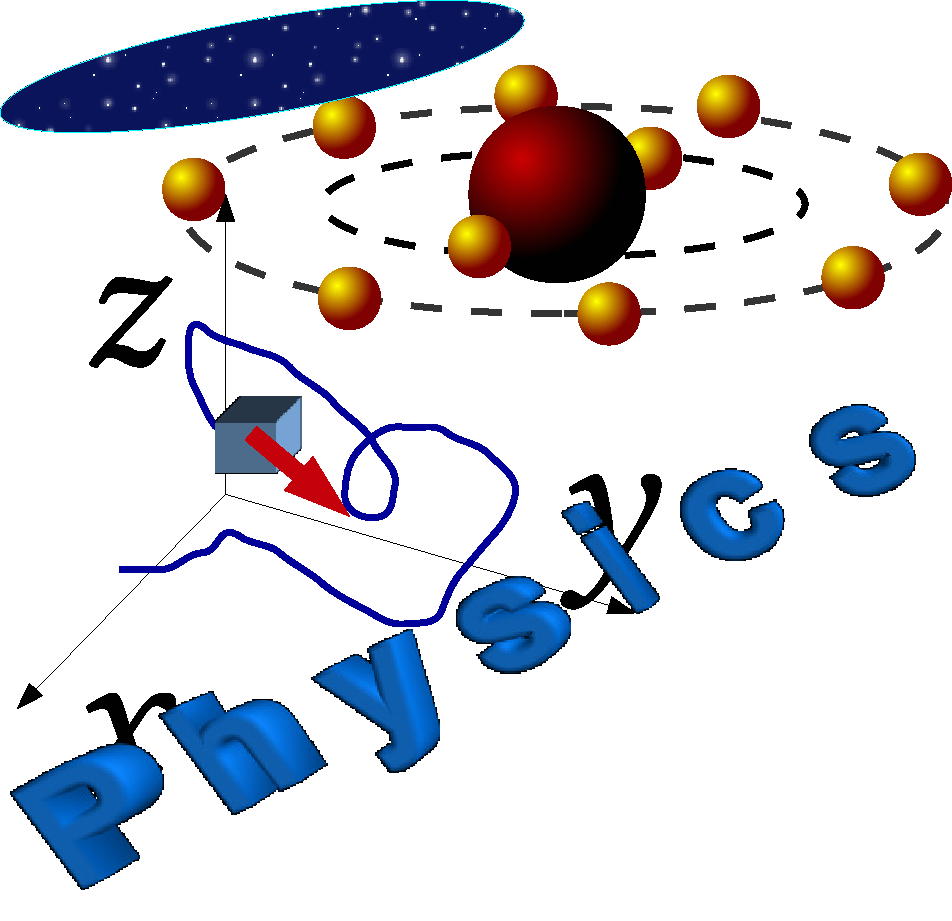
\includegraphics[keepaspectratio, width=6cm,height=3cm,clip]{hyoushi.pdf}}
    \par


    %========================
    % 索引作成の宣言
    %========================
      \makeindex

    %========================
    % 再定義(renewcommand)
    %========================
      %******************************************************************************
%  Newcommand
%******************************************************************************
%================================================
% * 章・節などの表示変更
%================================================
\renewcommand{\thesection}{\thechapter.\arabic{section}}
\renewcommand{\thesubsection}{\thesection.\arabic{subsection}}
\renewcommand{\tablename}{表\;}
\renewcommand{\figurename}{図\;}

\renewcommand{\bibname}{参考図書・教科書等}

%\renewcommand{\prechaptername}{第}
%\renewcommand{\postchaptername}{章}

\renewcommand{\labelenumi}{(\arabic{enumi})\;}
\renewcommand{\labelenumii}{(\alph{enumii})\;}
\renewcommand{\labelenumiii}{(\roman{enumiii})\;}
 %% - 一般の脚注のスタイル変更
%\renewcommand\thefootnote{$\mbox{}^{\clubsuit}$\kern1pt\arabic{footnote})\,} % パターン1: 三つ葉
\renewcommand\thefootnote{$\mbox{}^{\blacktriangleright}$\kern1pt\arabic{footnote})\,} % パターン2: 黒三角形
\renewcommand{\footnoterule}{%
  \vspace{1pt}                      % 線から上の幅
  \noindent\rule{0.25\textwidth}{0.5pt}   % 線の長さ,太さ
  \vspace{2pt}                     % 線から下の幅
}

\renewcommand{\textreferencemark}{\textreferencemark\,\,}
\newcommand{\komemark}{\textreferencemark}
 %% - 行間の調整
%\renewcommand{\baselinestretch}{1.05}%普通のx倍の行間間隔

%================================================
% * 演算子などの省略記述用
%================================================
% * ベクトル解析用の演算子
\newcommand{\drot}{\mathrm{rot}\,}
\newcommand{\ddiv}{\mathrm{div}\,}
\newcommand{\dgrad}{\mathrm{grad}\,}
% * ゼロベクトル
\newcommand{\bzero}{\textbf{0}}
% * 面積分
\newcommand{\sint}{\int\mspace{-11mu}\int}
% * 体積積分
\newcommand{\vint}{\int\mspace{-11mu}\int\mspace{-11mu}\int}
\newcommand{\OmegaS}{\Omega_{S}}
% * 微分記号(立った"d")
\newcommand{\df}{\,\mathrm{d}}
% * 偏微分記号
\newcommand{\rd}{\partial}
% * ダランべルシアン
\newcommand{\Dal}{\Box\,}
% * ラプラシアン
\newcommand{\Lap}{\triangle}
% * 自然対数の底
\newcommand{\e}{\mathrm{e}}
%\newcommand{\exp}{\mathrm{exp}}
% * 量子論的ハミルトニアン記号:$\qH$
\newcommand{\qH}{\mathcal{H}\,}
% * ラグランジアン密度
\newcommand{\qL}{\mathcal{L}\,}
% * 量子論的運動量演算子:$\dpx , \dpy , \dpz$
\newcommand{\dpx}{-i\hbar \frac{\partial}{\partial x}\,}
\newcommand{\dpy}{-i\hbar \frac{\partial}{\partial y}\,}
\newcommand{\dpz}{-i\hbar \frac{\partial}{\partial y}\,}
% * 量子論的エネルギー演算子:$\dE$
\newcommand{\dE}{i\hbar \frac{\partial}{\partial t}\,}
% * 量子論的ハミルトニアン演算子:$\dH$
\newcommand{\dH}{-i\hbar \nabla \,}
% * その他
\newcommand{\Shrps}{$\sharp\;$} % シャープ記号#
\newcommand{\Fig}{Fig\,\,} % 参照図を明示するときに使用する:ex.) 図\ref{xxx}
\newcommand{\Table}{図\,\,}
\newcommand{\circC}{${}^{\circ}$C}

%================================================
% * 標準的な画像のサイズ
%================================================
% 4:3 Default Size
\newcommand{\includegraphicsdefault}[1]{\includegraphics[keepaspectratio, width=4.00cm, height=3.00cm, clip]{#1}}
% 4:3 Middle Size
\newcommand{\includegraphicsmiddle}[1]{\includegraphics[keepaspectratio, width=6.00cm, height=4.5cm, clip]{#1}}
% 4:3 Large Size
\newcommand{\includegraphicslarge}[1]{\includegraphics[keepaspectratio, width=7.2cm, height=4.98cm, clip]{#1}}
% 2:1 Default Size
\newcommand{\includegraphicshalfmid}[1]{\includegraphics[keepaspectratio, width=6cm, height=3cm, clip]{#1}}
% 1:1 Squeare Default Size
\newcommand{\includegraphicssqmid}[1]{\includegraphics[keepaspectratio, width=4.00cm, height=4.00cm, clip]{#1}}
% 1:1 Squeare Default Size
\newcommand{\includegraphicssqmlrg}[1]{\includegraphics[keepaspectratio, width=7.2cm, height=7.2cm, clip]{#1}}

% Two Graphics Size
\newcommand{\includegraphicsdouble}[1]{\includegraphics[keepaspectratio, width=3.2cm, height=2.4cm, clip]{#1}}


%================================================
% * アルファベットの太字(ベクトルとか)
%================================================
\newcommand{\ba}{\boldsymbol{a}}
\newcommand{\bb}{\boldsymbol{b}}
\newcommand{\bc}{\boldsymbol{c}}
\newcommand{\bd}{\boldsymbol{d}}
\newcommand{\be}{\boldsymbol{e}}
\newcommand{\bg}{\boldsymbol{g}}
\newcommand{\bldf}{\boldsymbol{f}}
\newcommand{\bj}{\boldsymbol{j}}
\newcommand{\bp}{\boldsymbol{p}}
\newcommand{\br}{\boldsymbol{r}}
\newcommand{\bv}{\boldsymbol{v}}
\newcommand{\bx}{\boldsymbol{x}}
\newcommand{\by}{\boldsymbol{y}}
\newcommand{\bz}{\boldsymbol{z}}
\newcommand{\bn}{\boldsymbol{n}}
\newcommand{\bE}{\boldsymbol{E}}
\newcommand{\bF}{\boldsymbol{F}}
\newcommand{\bC}{\boldsymbol{C}}
\newcommand{\bB}{\boldsymbol{B}}
\newcommand{\bA}{\boldsymbol{A}}
\newcommand{\bi}{\boldsymbol{i}}
\newcommand{\bt}{\boldsymbol{t}}
\newcommand{\bk}{\boldsymbol{k}}
\newcommand{\bl}{\boldsymbol{l}}
\newcommand{\bS}{\boldsymbol{S}}
\newcommand{\bI}{\boldsymbol{I}}
\newcommand{\bH}{\boldsymbol{H}}
\newcommand{\bP}{\boldsymbol{P}}
\newcommand{\bD}{\boldsymbol{D}}
\newcommand{\bX}{\boldsymbol{X}}
\newcommand{\bY}{\boldsymbol{Y}}
\newcommand{\bL}{\boldsymbol{L}}
\newcommand{\bM}{\boldsymbol{M}}
\newcommand{\bN}{\boldsymbol{N}}
\newcommand{\bo}{\boldsymbol{o}}
\newcommand{\bU}{\boldsymbol{U}}
\newcommand{\bV}{\boldsymbol{V}}
\newcommand{\bW}{\boldsymbol{W}}
\newcommand{\bZ}{\boldsymbol{Z}}
\newcommand{\setN}{\mathbb{N}}
\newcommand{\setC}{\mathbb{C}}
\newcommand{\setZ}{\mathbb{Z}}
\newcommand{\setR}{\mathbb{R}}
\newcommand{\setA}{\mathbb{A}}
\newcommand{\setB}{\mathbb{B}}
\newcommand{\setD}{\mathbb{D}}
\newcommand{\setE}{\mathbb{E}}
\newcommand{\setF}{\mathbb{F}}
\newcommand{\bldi}[1]{\textit{\textbf{{#1}}}}
\newcommand{\bld}[1]{\textbf{{#1}}}

%================================================
% * 花文字
%================================================
\newcommand{\flwA}{\mathcal{A}}
\newcommand{\flwB}{\mathcal{B}}
\newcommand{\flwC}{\mathcal{C}}
\newcommand{\flwD}{\mathcal{D}}
\newcommand{\flwE}{\mathcal{E}} % 起電力
\newcommand{\flwF}{\mathcal{F}} % 一般化された力とか
\newcommand{\flwH}{\mathcal{H}} %
\newcommand{\flwp}{\mathcal{p}} % 一般化された運動量
\newcommand{\flwL}{\mathcal{L}}

%================================================
% * ギリシア数字作成
%================================================
\newcommand{\I}{I}
\newcommand{\II}{I\hspace{-.1em}I}
\newcommand{\III}{I\hspace{-.1em}I\hspace{-.1em}I}
\newcommand{\IV}{I\hspace{-.1em}V }
\newcommand{\V}{V}
\newcommand{\VI}{V\hspace{-.1em}I}
\newcommand{\VII}{V\hspace{-.1em}I\hspace{-.1em}I}
\newcommand{\VIII}{V\hspace{-.1em}I\hspace{-.1em}I\hspace{-.1em}I }
\newcommand{\X}{X}
%再定義1(数式番号の表現 chap-sub-subsub)
%\makeatletter
% \renewcommand{\theequation}{%
  % \thesection.\arabic{equation}}
  %\@addtoreset{equation}{section}
 %\makeatother

%================================================
% * 新しいカウンタの生成
%================================================
% * 宣言
\newcounter{Memo}           %
\newcounter{Snumber}        % "memo" の番号
\newcounter{myshade}        % 物理部分の重要事項の番号
\newcounter{PreAttentionNo} % 記入方法の諸注意の番号
\newcounter{AboutThisNoteNo}% 「このノートにいて」の番号
% * 初期値設定
\setcounter{Memo}{1}
\setcounter{Snumber}{1}
\setcounter{myshade}{1}
\setcounter{PreAttentionNo}{1}
\setcounter{AboutThisNoteNo}{1}

%================================================
% * カウンタの再設定
%================================================
% * 目次の表示の深さを設定する
\setcounter{secnumdepth}{6}
\setcounter{tocdepth}{4}
% * 立て揃え で改行を許す:0から4まで
%    0      ; 絶対改行しない
%    1から3 ; 適度に改行する.数字が高いほど,
%             基準が緩くなる
%    4      ; 必ず改行する
\allowdisplaybreaks[4]

%================================================
% 図のcaptionの : をとる
%================================================
\makeatletter
\long\def\@makecaption#1#2{%
\vskip\abovecaptionskip%
%\sbox\@tempboxa{#1: #2}% <--- original
\sbox\@tempboxa{#1\;\; #2}
\ifdim \wd\@tempboxa >\hsize%
%#1: #2\par <--- original
#1 #2\par
\else
\global \@minipagefalse
\hb@xt@\hsize{\hfil\box\@tempboxa\hfil}%
\fi
\vskip\belowcaptionskip}
\makeatother
%------------------------------------------------

%******************************************************************************
%  Newtheorem
%******************************************************************************
%定義や定理の出力は,newtheorem 環境を使用します.
%定義の場合,プリアンブルに次の内容を記述します.
%
%\newtheorem{dfn}{Definition}[引数]

%「定義」と表示させたい場合は,
%Definition を 定義 に書き換えます.
%
%定義番号に (2.1) のように章番号をつけたい場合は,
%引数に,[chapter]を入力します.
%章立ての文書で (1.3.2) のように節番号を付けたい場合は,
%引数にsection を入力します.
%
%% 使い方:定理の場合
%\begin{thm}
%集合 $A, B$ について,$A$ から $B$ への単射および $B$ から $A$ への単射がともに
%存在すれば,$A$ と $B$ の濃度が等しい.
%\end{thm}
\theoremstyle{plain}
\newtheorem{thm}{定理}[section]
\newtheorem{lem}{補題}[section]
\newtheorem{cor}{系}[section]
\newtheorem{prp}{命題}[section]
%
\theoremstyle{definition}
\newtheorem{dfn}{定義}[section]
%
\theoremstyle{remark}
\newtheorem{rem}{注意}
\newtheorem{prf}{証明}

%******************************************************************************
% Newenvironment
%******************************************************************************
% * Environment: \memo
\newenvironment{memo}[1]
{ % before
    \addcontentsline{toc}{subsubsection}{\Shrps\textit{memo} No.\theSnumber : #1} % 目次
    \subsubsection*{\Shrps\textit{memo} No.\theSnumber : \emph{#1}}
    %\addcontentsline{toc}{subsubsection}{\;\;\;\Shrps\textit{memo} \; #1}
    %\subsubsection*{\;\;\;\Shrps\textit{memo} \;\;\; \emph{#1}}
    \stepcounter{Snumber}
    \small
}
{ % after
    \par \normalsize
}

% * Environment: \myshadebox
\newenvironment{myshadebox}[1]
{ % before
    %\addcontentsline{toc}{subsubsection}{\;\S\;Point No.\themyshade :\; #1} % 目次
    \leavevmode \\  \leavevmode \\
    \begin{shadebox}
        %\;\textbf{\ding{42}\;Point No.\themyshade :\, #1} \leavevmode \\
                \textbf{\;Point \themyshade :\, \textbf{#1}} \vspace{1mm} \\
        \leavevmode
        \stepcounter{myshade}
}
{ % after
    \end{shadebox}
    \leavevmode \\
}

% * Environment: \comment
\newenvironment{mycomment}
{ % before
    \par \small
    \textbf{コメント$\quad$}
}
{ % after
    \newline \par \normalsize
}

% * Environment: \mysmallsec
\newenvironment{mysmallsec}[1]
{ % before
%    \addcontentsline{toc}{subsubsection}{\$ #1} % 目次
%    \subsubsection*{\$ #1}
    \subsubsection*{\P \; #1}
}

% * Environment: \pre_attention
\newenvironment{preattention}[1]
{ % before
    \addcontentsline{toc}{section}{(\thePreAttentionNo) #1} % 目次
    \subsubsection*{(\thePreAttentionNo) \emph{#1}}
    \stepcounter{PreAttentionNo}
    \label{my:preattention:#1}
}
{ % after
}

% * Environment: \aboutthisnote
\newenvironment{aboutthisnote}[1]
{ % before
    %\addcontentsline{toc}{section}{\$\theAboutThisNoteNo #1} % 目次
    \subsubsection*{\$\theAboutThisNoteNo \emph{#1}}
    \stepcounter{AboutThisNoteNo}
    \small
}
{ % after
    \par \normalsize
}
%独自コマンドの設定・既存コマンド変更の設定

    %========================
    % レイアウト(共通)
    %========================
    %******************************************************************************
%  TeX Layout ( A4 Paper version )
%******************************************************************************
%数式のフォントの選択
%\usepackage{txfonts}
%\usepackage{pxfonts}
%\usepackage[T1]{fontenc}
%\usepackage{lmodern}

%英文文字フォントの選択
%\usepackage{timesnew} %Times new Roman

%ページ番号全体の非表示化
%\pagestyle{empty}

%文書レイアウト
\setlength{\topmargin}{-10mm}
\setlength{\textwidth}{155mm}
\setlength{\textheight}{256mm}
\setlength{\oddsidemargin}{15mm}
\setlength{\evensidemargin}{-10mm}
        %フッタ,ヘッダと本文との行間の調整
\setlength{\headsep}{2zw}
\setlength{\footskip}{1zw}

\setlength{\parindent}{1zw} % 段落先頭のスペース zw...全角1文字単位
\setlength{\parskip}{0.4zw} % 段落間スペース

%\renewcommand{\baselinestretch}{0.9}%普通のx倍の行間間隔
%\raggedbottom

%テキストのレイアウトの設定

    %========================
    % レイアウト(固有)
    %========================
    %\setlength{\columnseprule}{0.2mm}
    \setstretch{1.2}
    \setlength{\columnsep}{2zw}
    \setlength{\mathindent}{1zw}

%%*=*=*=*=*=*=*=*=*=*=*=*=*=*=*=*=*=*=*=*=*=*=*=*=*=*=*=*=*=*=*=*=*=*=*=*=*=*%%
%%                             本             文
%%*=*=*=*=*=*=*=*=*=*=*=*=*=*=*=*=*=*=*=*=*=*=*=*=*=*=*=*=*=*=*=*=*=*=*=*=*=*%%
\begin{document}
    %========================
    % 前処理
    %========================
      
    %===========================================================================
    % * 表紙作成
    %===========================================================================
        \maketitle
        \pagenumbering{roman} %ページ番号の数字をローマ数字にする
        \setcounter{page}{2}  %表紙のじベージに空白ページ挿入

    %===========================================================================
    % * まえおき「このノートについて」の挿入
    %===========================================================================
        \frontmatter %まえおきであることの宣言
        \addcontentsline{toc}{chapter}{\textbf{このノートについて}}
        \section*{このノートについて}
\begin{aboutthisnote}{作成方法}
    \textbf{このノートの作成にはp\LaTeXe を使用させて頂きました}.
\end{aboutthisnote}

\begin{aboutthisnote}{作成動機}
    このノートを作ることにしたのは,
    将来の自分のためです.おそらく,
    今学習している『物理学』の内容を
    忘れてしまっていると思うので,
    その記録をしておこうというものです.
\end{aboutthisnote}

\begin{aboutthisnote}{内容についての重要な注意}
    このノートの内容は
    教科書を読んだ直後に
    書いたものなので,
    教科書の内容そのままである部分が大半です.
    つまり,私のオリジナルではなく,
    様々な教科書をつぎはぎしたものです.
    しかし,(一部の引用を除いて)教科書の丸写しではなく,私なりにその内容を
    解釈して記述していますので,その教科書の内容の正確さが失われてる
    可能性があります.
    何か変な点,矛盾する箇所等があった場合は,
    すぐにその内容を修正するようにして下さい.
\end{aboutthisnote}

\begin{aboutthisnote}{言い訳}
    物理学は教科書がたくさんあり,
    また,趣味で物理学をなさっていて
    Websiteを開いている方々も多いです.
    このノートの内容はほとんどが教科書やWebによるものです.
    しかしそれでも,人から聞いたり本で読んだりした知識ではありますが,
    その知識を自分なりにノートという形でまとめることで自分の中で再定式化できれば,
    新しいものの見方を発見できるかもしれないと思い本ノートの作成を続けています.
\end{aboutthisnote}

\begin{aboutthisnote}{補足}
    このノートは物理学の理論だけを記述しており,その具体的なことは書いていないことが多いです.
    具体例を考えることで,その法則の意味をより深く理解することができますが,
    具体例は割愛しています.しかし,書かないからといって,重要でないということでは決してありません.
    具体的な問題を演習することは,例えば,定義された物理量の
    直感的な把握や,大体の大きさの見当をつけるのに役に立ちます.また,
    複数の法則の結びつき方を感じ取ることもできます.
    従って,具体例は必ず演習書等を用いて,考えなければいけません.
    理論だけ読んでいても,本当にその理論が現実と一致するかどうかは,多くの場合,
    演習を通してでしか確認できません.
    学校や科学館などでもない限り,実験して確かめるということは難しいことが多いのです.
    まあ,理論を読んで満足ができるわけがないことは当たり前なのですが(法則の現実性を
    “実感”しない限り,その法則は私にとって,確かなものではないから),
    演習をおろそかにしがちな自分に注意するために,ここに書いておきました.
\end{aboutthisnote}

\begin{aboutthisnote}{挿入図について}
    図の多くは,寺嶋容明さん
    の作られた「EPS-draw」を用いて,私が作図したものです.
    また,LibreOfficeのDrawで作図したものもあります.
    グラフの作成は,PerlやPythonにより数値計算をして,
    LibreOfficeのcalcで図式化しています.
    gnuplotで書いたところもあります.
    曲面の作成にはフリーの数式処理ソフトmaximaを使って作成
    しているところもあります.
\end{aboutthisnote}

\begin{aboutthisnote}{内容を鵜呑みにしないで下さい}
    このノートはド素人が書いたものであり,正確である保証はありません.
    むしろ,間違っている所があることは確実でしょう.
    特に,計算ミスに不安を感じます.見つけ次第,訂正していきます.
\end{aboutthisnote}

\begin{aboutthisnote}{これはノートです}
    このノートは教科書風の体裁を取っていますが,あくまでも学習ノートです.
    従って,項目の配置は論理的ではありません.メモ書き程度のものです.
\end{aboutthisnote}

\begin{aboutthisnote}{記載順}
    物理学の内容を学習する目的で,このノートをはじめから読もうとしても,
    その内容に行き着くまでには時間がかかることと思います.
    数学の学習と物理学の考え方などが,物理学の前提知識として,先立って
    説明されているからです.
    なので,そういった読み方をしてしまうと,挫折してしまうでしょう.
    このノートの使い方として,まずは目次をみて,参照したい部分を
    見つけて読む,という方法が良いと思います.
\end{aboutthisnote}

\begin{aboutthisnote}{記述精神}
    できるだけ,詳しく書こうと思います.式変形も省略なしにしたいです.
    さらにできることなら,将来,このノートを参考に,理解した物理学を論理的に自身の
    中で再構成した文書を作りたいです.
\end{aboutthisnote}

\begin{aboutthisnote}{脚注の多さについて}
    ノートを記載していた時の心境を脚注に書いておく.
    あとで,なんでそのような記述をしたかを思い起こすヒントになるはず.
    脚注が多すぎて読みにくくなってしまうが,ノートなのでいくら汚く
    書いてもOKとしたい.
\end{aboutthisnote}

\begin{aboutthisnote}{願望}
    私は,物理学を“習得”しようとは考えていません.私にとって物理学の学習は趣味です.
    物理学を勉強する理由は,それを使えるようにするためではなく,物理法則を知りたいからです.
    自然はどのように成立しているのか.自分なりに,物理学を実感したいのです.
    ですので,このノートは単に物理学の表面しか,記述していません
        \footnote{
            もしかしたら,表面もすらも記述していないかもしれない,という不安があります.
        }.

    このノートを書くことが生涯の趣味になることを期待しています.
\end{aboutthisnote}

%%%%\begin{aboutthisnote}{このノートの目標}
%%%%    最後に,学習のひそかな到達目標について.このノートの到達
%%%%    目標を“超電導”にしたいと考えています.卒研の内容が超電導現象に
%%%%    関する実験的なことだったので,理論的な事も知りたいからです.
%%%%    ただ,超電導はとても難しいので,そこに到達できるかどうかは
%%%%    わかりません...
%%%%
%%%%    また,パソコンの動作を物理学から理解したいという願望(私にとっては野望)もある.
%%%%
%%%%\end{aboutthisnote}

    以下,文の読みやすさと文字数のことを考えて,丁寧語による記述をやめます.


    %===========================================================================
    % * まえおき「このノートで使用する記号」の挿入
    %===========================================================================
        \newpage
        \addcontentsline{toc}{chapter}{\textbf{このノートで使用する記号}}
        \section*{このノートで使用する記号}
    このノートで使用する記号について,
    以下に示しておく.
    ノートを読んでいて分からくなった記号
    があったら,これを参考にしてもらいたい.
    もちろん,用語については本文を参照にすること.

    複数の意味で使われる記号がいくつもあるが,
    それらについてはスラッシュ / で区切りをいれた.

    % [約束] 一行に収まる程度(30文字程度)で説明すること(体裁のため)

    %===========================================================
    % * アルファベット(斜太字:大文字)
    %===========================================================
    \subsubsection*{アルファベット(太字:大文字)}
    \begin{tabular}{lll}
        $\bE$                   &:  & 電場                                                                  \\
        $\bA$                   &:  & ベクトルポテンシャル                                                  \\
        $\bB$                   &:  & 磁束密度                                                              \\
        $\bI$                   &:  & 電流                                                                  \\
        $\bD$                   &:  & 電束密度                                                              \\
        $\bH$                   &:  & 磁場                                                                  \\
        $\bP$                   &:  & 誘電分極                                                              \\
        $\bL$                   &:  & 角運動量                                                              \\
        $\bN$                   &:  & 回転力(トルク)                                                      \\
        $\bF$                   &:  & 力(合成力)                                                          \\
        $\bM$                   &:  & 磁化                                                                  %\\
    \end{tabular}

    %===========================================================
    % * アルファベット(斜太字:小文字)
    %===========================================================
    \subsubsection*{アルファベット(太字:小文字)}
    \begin{tabular}{lll}
        $\br$                   &:  & 位置,$(\,x,\,y,\,z\,)$ と同じ.                                      \\
        $\bv$                   &:  & 速度,$(\,v_{x},\,v_{y},\,v_{z}\,)$ と同じ                            \\
        $\ba$                   &:  & 加速度,$(\,a_{x},\,a_{y},\,a_{z}\,)$ と同じ                          \\
        $\bp$                   &:  & 運動量,$(\,p_{x},\,p_{y},\,p_{z}\,)$ と同じ                          \\
        $\bi$                   &:  & 電流密度,$(\,i_{x},\,i_{y},\,i_{z}\,)$ と同じ                        \\
        $\bldf$                 &:  & 分解された力                                                          %\\
    \end{tabular}

    %===========================================================
    % * アルファベット(斜細字:大文字)
    %===========================================================
    \subsubsection*{アルファベット(細字:大文字)}
    \begin{tabular}{lll}
        $G$                     &:  & 万有引力定数,または,重力定数                                        \\
        $U$                     &:  & ポテンシャルエネルギー                                                \\
        $T$                     &:  & 運動エネルギー/張力                                                   \\
        $E$                     &:  & 全エネルギー/電場の大きさ                                      \\
        $U$                     &:  & ポテンシャル/内部エネルギー                                 \\
        $L$                     &:  & 角運動量/ラグランジアン                                               \\
        $I$                     &:  & 力積/電流の大きさ                                              \\
        $S$                     &:  & 面積/任意の閉曲面                                                     \\
        $V$                     &:  & 体積                                                                  \\
        $O$                     &:  & 原点                                                                  \\
        $H$                     &:  & ハミルトニアン/磁場の大きさ                            %\\
    \end{tabular}

    %===========================================================
    % * アルファベット(斜細字:小文字)
    %===========================================================
    \subsubsection*{アルファベット(細字:小文字)}
    \begin{tabular}{lll}
        $l$                     &:  & 長さ/任意の閉曲線                                                     \\
        $m$                     &:  & 質量(慣性質量と重力質量)                                                   %\\
    \end{tabular}

    %===========================================================
    % * アルファベット(添字付き)
    %===========================================================
    \subsubsection*{アルファベット(添字付き)}
    \begin{tabular}{lll}
        $m_{\mathrm{i}}$        &:  & 慣性質量                                                              \\
        $m_{\mathrm{g}}$        &:  & 重力質量                                                              \\
        $S_{l}$                 &:  & 任意の閉曲線 $l$ を縁とする曲面                   \\
        $k_{B}$                 &:  & ボルツマン定数                                                        %\\
    \end{tabular}

    %===========================================================
    % * アルファベット(立太字:大文字)
    %===========================================================

    %===========================================================
    % * アルファベット(立太字:小文字)
    %===========================================================

    %===========================================================
    % * アルファベット(立細字:大文字)
    %===========================================================
    \subsubsection*{アルファベット(立細字:大文字)}
    \begin{tabular}{lll}
        K                       &:  & 任意の慣性系                                                          \\
        K$'$                    &:  & Kとは別の任意の慣性系                                                 %\\
    \end{tabular}

    %===========================================================
    % * アルファベット(立細字:小文字)
    %===========================================================

    %===========================================================
    % * 花文字
    %===========================================================
    \subsubsection*{花文字}
    \begin{tabular}{lll}
        $\qL$                   &:  & ラグランジアン密度                                                    \\
        $\qH$                   &:  & 量子論ハミルトニアン演算子                                            \\
        $\flwF$                 &:  & 一般化された力                                                        \\
        $\flwE$                 &:  & 起電力                                                                %\\
    \end{tabular}

    %===========================================================
    % * ギリシア文字(大文字)
    %===========================================================
    \subsubsection*{ギリシア文字(大文字)}
    \begin{tabular}{lll}
        $\Sigma$                &:  & 総和の記号                                                            \\
        $\Omega$                &:  & 任意の領域の内部                                 %\\
    \end{tabular}

    %===========================================================
    % * ギリシア文字(小文字)
    %===========================================================
    \subsubsection*{ギリシア文字(小文字)}
    \begin{tabular}{lll}
        $\gamma$                &:  & ローレンツ因子                                                        \\
        $\nu$                   &:  & 周波数                                                                \\
        $\rho$                  &:  & 電荷密度/電気抵抗率                                                   \\
        $\sigma$                &:  & 電気伝導率                                                            \\
        $\phi$                  &:  & 電気的なポテンシャルエネルギー                                        %\\
    \end{tabular}

    %===========================================================
    % * ギリシア文字(添字付き)
    %===========================================================
    \subsubsection*{ギリシア文字(添字付き)}
    \begin{tabular}{lll}
        $\Omega_{S}$            &:  & 任意の閉曲面の内側の領域                         %\\
    \end{tabular}

    %===========================================================
    % * 数式記号
    %===========================================================
    \subsubsection*{数式記号の意味}
    $\bA$,$\bB$ は一般の(特に意味を与えない)ベクトルであるとする.
    $\br$ は位置ベクトル,$\bt$ は線素ベクトル,$\bS$ は面素ベクトルとする.
    また,$f(x)$ は $x$ を独立変数とする一次関数であり,
    $f(x,\,y,\,\cdots)$ は $(x,\,y,\,\cdots)$ を独立変数とするとする多変数関数である.\\

    \begin{tabular}{lll}
            $\bA \perp \bB$                                         &:  & $\bA$ は $\bB$ に \textbf{垂直}                          \\
            $\bA \parallel \bB$                                     &:  & $\bA$ は $\bB$ に \textbf{平行}                          \\
            $\bA_{\perp \bB}$                                       &:  & $\bA$ の $\bB$ に \textbf{垂直な成分}                    \\
            $\bA_{\parallel \bB}$                                   &:  & $\bA$ の $\bB$ に \textbf{平行な成分}                    \\
            $\displaystyle \int f(x) \df x$                         &:  & 積分         \\
            $\displaystyle \oint f(\br) \cdot \df \bt$              &:  & 線積分        \\
            $\displaystyle \sint f(\br) \cdot \df \bS$              &:  & 面積分        \\
            $\displaystyle \vint f(\br) \df V$                      &:  & 体積積分      \\
            $\df f$                                                 &:  & 微分/全微分     \\
            $\displaystyle \frac{\df}{\df x} f(x)$                  &:  & 導関数          \\
            $\displaystyle \frac{\rd}{\rd x} f(x,\, y,\, \cdots)$   &:  & 偏微分      \\
    \end{tabular}

    %===========================================================
    % * 行内に書く場合の,演算子について
    %===========================================================
    \subsubsection*{行内に書く場合の演算子の形}
        \begin{tabular}{lll}
            $ab/cd$                 &:  & $\displaystyle \frac{ab}{cd}$ を文中で記す場合.            \\
            $(a/b)(c/d)$            &:  & $\displaystyle \frac{a}{b}\frac{c}{d}$ を文中で記す場合.   \\
            $\sum_{n=1}^{N}$        &:  & $\displaystyle \sum_{n=1}^{N}$ を文中で記す場合.           \\
            $\bigcap_{n=1}^{N}$     &:  & $\displaystyle \bigcap_{n=1}^{N}$ を文中で記す場合.        \\
            $\bigcup_{n=1}^{N}$     &:  & $\displaystyle \bigcup_{n=1}^{N}$ を文中で記す場合.        \\
            $\int$                  &:  & $\displaystyle \int$ を文中で記す場合.                     \\
            $\sint$                 &:  & $\displaystyle \sint$ を文中で記す場合.                    \\
            $\vint$                 &:  & $\displaystyle \vint$ を文中で記す場合.                    \\
    \end{tabular}




    %===========================================================================
    % * まえおき「内容概略」の挿入
    %===========================================================================
        \newpage
        \addcontentsline{toc}{chapter}{\textbf{記述する内容(予定)}}
        \section*{記述する内容(予定)}

学習の内容(予定)は,以下の通りである.
\begin{center}
\begin{description}
    \item[第1部「{\bf 古典力学}」] \mbox{} \\
        \textbf{古典力学} とは,\textbf{ニュートン力学} と \textbf{解析力学} の
        総称である.第1章のニュートン力学では,物体の運動法則とその記述方法,推
        論方法を学ぶ.第2章の解析力学は,ニュートン力学を数学的に整理したもので
        ある.

    \item[第2部「{\bf 電磁気学}」] \mbox{} \\
        電磁気学は,その名の通り,電気と磁気に関する学問である.
        電気と磁気の関係は深い.このことについて学習する.

    \item[第3部「{\bf 特殊相対性理論}」] \mbox{} \\
        自分が光の速さで動けるとしよう.このとき,どのような世界が待っているだろうか.

    \item[第4部「{\bf 熱・統計物理学}」] \mbox{} \\
        熱とは何か.熱をどのように捉えるべきか.

    \item[第5部「{\bf 量子力学}」] \mbox{} \\
        原子のスケール($10^{-10}$[m])で物理法則を考えるとき,
        古典力学では扱えない現象が生じる.原子レベルの世界の
        物理法則をここで確認する.

    \item[第6部「{\bf 一般相対性理論}」] \mbox{} \\
        特殊相対性理論では慣性系を仮定しているが,
        実際は重力の存在のために,完全な慣性系は存在しない.
        重力の存在する場を扱う理論.

\end{description}
\end{center}

なお,参考にした教科書等については,
このノートの最後にまとめて書いておく.



    %===========================================================================
    % * まえおき「記述方法についての諸注意」の挿入
    %===========================================================================
        \newpage
        \addcontentsline{toc}{chapter}{\textbf{記述方法についての諸注意}}
        \section*{記述方法についての諸注意}
    \begin{mycomment}
        ノートの記述に先立って,数式の記述についていくつか注意しておきたい.
        意味が分からなければ,先に進んでも構わないが,この部分に数式表現
        の注意があることは覚えておいてもらいたい(必要な場合に,ここを参照
        できるように).
    \end{mycomment}


    %===========================================================
    % * 括弧の扱いについて
    %===========================================================
    \begin{preattention}{括弧の扱いについて}
        このノートでは,多くの教科書と同様に,関数の独立変数を表す括弧「例:$\phi(x)$」と
        式中の括弧「例:$a(b+c)$」は同一のものを使用している.

        しかし,この表記は,ときには,誤解をまねく.というのも,
        例えば,関数 $\phi(x)$ と $a+b$ の積を記述する場合,
            \begin{equation*}
                \phi(x) (a+b)
            \end{equation*}
        と書く.これは見方によっては,実数 $\phi$,$x$,$a+b$ の積
        であると解釈することもできる.まあ,この場合は $x$ が1つであること
        から,「$x$ は関数 $\phi$ の独立変数であり,$\phi(x)$ は関数を表すのだな」
        と読まれることだろう.しかし,上の独立変数 $x$ に定数 $a+b$ を代入すること
        きには,曖昧にな記述になってしまう.つまり,
            \begin{equation*}
                \phi(a+b) (c+d)
            \end{equation*}
        これは,著者の意図としては,「関数 $\phi$ の独立変数 $x$ に,$a+b$ を代入したものと,
        実数 $c+d$ の積」を表現したつもりだろう.しかし,読者が分からしてみれば,単に式を
        見ただけでは,「3つの実数 $\phi$,$a+b$,$c+d$ の積」と解釈するのが妥当である.
        もちろん,著者は,このような式を記述する前後で,文字の意味に対する説明を行って
        いるので,通常なら,誤解されることはない.しかしながら,意味が曖昧な式である
        ことには変わりはない.それゆえに,何かストレスを感じてしまう.

        ちなみに,「関数 $\phi$ の独立変数 $x$ に,$a+b$ を代入したものと,
        実数 $c+d$ の積」を表現したい場合には,
            \begin{equation*}
                \phi(a+b) \cdot (c+d) \quad \mbox{, あるいは,} \quad (c+d)\phi(a+b)
            \end{equation*}
        などと書かき,区別を強調するかもしれない.何れにしても,教科書に記述されている
        ことを理解するのは読者の仕事であり,臨機応変に適切に読み込まなければいけない.
        それでも尚,複数の意味として捉えられてしまうようであれば,もしそれが重要な部分
        であると感じるなら,著者に直接質問すべきだ.しかし,著者と直接対話できる
        ことは容易ではなく,また,趣味で物理学を学んでいるので実害はなく,直接質問
        することを躊躇してしまうことだと思う.そういった場合は,手っ取り早い方法として,
        他の著作も参照して見ることである.大概の場合は,この方法で解決することだろう.


    \end{preattention}

    %===========================================================
    % * 積分記号について
    %===========================================================
    \begin{preattention}{積分記号}
        おそらく,一般的な積分の表現は,
            \begin{align*}
                \int f(x) \df x
            \end{align*}
        のように,関数 $f(x)$ をインテグラル $\int$ と微分記号 $\df x$ で
        囲んだ形だろう.このノートでも,積分を表す記述方法として,上記を採用する.

        しかし,別の表記方法を採用している教科書も多い.次のような
        書き方がされることがあるのだ.
            \begin{align*}
                \int \df x f(x).
            \end{align*}
        この書き方は,\textbf{演算子} という考え方をもとにした
        表現方法である.

        演算子とは何かを,考えてみよう.微分を例にとろう.関数 $f(x)$ を $x$ で
        微分することを,次のように表現する.
            \begin{align*}
                \frac{\df f(x)}{\df x}.
            \end{align*}
        上の表現とは別に,教科書には次のようにも表現されることが,書かれている
            \footnote{
                微積分の教科書であれば,どのようなものでも記述されている.
                もっと強い言い方をすれば,この記述を紹介していないものは,
                微積分の教科書とは言えない.
            }.
            \begin{align*}
                \frac{\df}{\df x} f(x).
            \end{align*}

        微分は,関数 $f(x)$ に対するひとつの操作である.具体的に見てみよう.
        例えば,$f(x)=x^{2}$ でれば,$f(x)$ を微分した結果 $f'(x)$ は $2x$ と
        なる.$f(x)=x^{5}$ であれば,$f'(x)=5x^{4}$ だし,$f(x)=\sin x$ だったら,
        $f'(x)=\cos x$ である.こうしてみると,微分するということは,元となる
        関数 $f(x)$ に対して,「微分するという操作」を与えることで,あたらな関数
        (導関数:$f'(x)$)を作り出していると,捉え直すことができる.こう考えた場合,
        上に書いた記号で,$\df/\df x$ の部分と,$f(x)$ の部分に分けてみて,
        「$x$ に関して微分するという操作 $\df/\df x$ を,関数 $f(x)$ に対して行う」
        と読むことで,$\df/\df x$ に,「$x$ に関して微分する」
        という意味を与えることができる.
        つまり,以下の記号
            \begin{align*}
                \frac{\df}{\df x}
            \end{align*}
        が,微分の操作を象徴する記号になる.$\df/\df x$ は,関数 $f(x)$ に対して微分するという
        作用をほどこすことから,\textbf{微分作用素} とよばれる.

        積分に関しても,微分と同様に考えて,一般的な記号 $\int f(x) \df x$ を書き換えて,
            \begin{align*}
                \int \df x f(x)
            \end{align*}
        とすることにより,積分という操作 $\int \df x$ を,関数 $f(x)$ に関して行う,といった
        意味を強調できる.
    \end{preattention}

    %===========================================================
    % * 三角関数の表現
    %===========================================================
    \begin{preattention}{三角関数の表現}
        ここで上げる問題は,上記の括弧の使い方に関連するものだが,
        三角関数に関する括弧の扱いについて,誤解を生みやすいので,
        ここで特別に取り上げることとする.

        三角関数は,$\sin x$ のように記述される.$x$ は位相とよばれ,
        この関数の独立変数をになっている.問題は,この位相 $x$ の書き方
        である.例えば,物理学では,位相として,角周波数 $\omega$ と時間 $t$ の
        積 $\omega t$ が使われることが多い.
        つまり,$x=\omega t$ として,
            \begin{equation*}
                \sin \omega t
            \end{equation*}
        と記述されることがある.ここまでは,特に問題がない.しかし,
        例えば,$\omega=\omega_{0}+\omega_{1}$ というような場合,上式は
            \begin{equation*}
                \sin \left(\omega_{0}+\omega_{1}\right) t
            \end{equation*}
        と書かれる.さて,この式はどう見えるだろうか.一般的な解釈
        では,位相が $\left(\omega_{0}+\omega_{1}\right) t$ の $\sin$ 関数
        だろう.しかし,式だけを見る限り,$\sin \left(\omega_{0}+\omega_{1}\right)$ と
        時間 $t$ の積であるようにも,解釈ができる.つまり,
            \begin{equation*}
                \{\sin \left(\omega_{0}+\omega_{1}\right)\}\cdot t
            \end{equation*}
        のようにも見えてしまうのである.しかし,このように見てしまうのは,
        暗黙の了解を知らないものだけである.三角関数を記述する上での暗黙の了解とは,
        $\sin$ の直後に記述されるものが位相である,ということである.つまり,
            \begin{equation*}
                \{\sin \left(\omega_{0}+\omega_{1}\right)\}\cdot t
            \end{equation*}
        と解釈してはいけない.あくまでも,位相は $\sin$ の直後に書かれている
        もじであり,この例では,$\left(\omega_{0}+\omega_{1}\right) t$ がその
        位相にあたる.ただし,$\sin x$ 全体が括弧に囲まれていて,例えば,
            \begin{equation*}
                \{\sin \left(\omega_{0}+\omega_{1}\right) t\}x
            \end{equation*}
        と書かれていたら,$\sin \left(\omega_{0}+\omega_{1}\right) t$ と $x$ の
        積であると解釈すべきだ.

        三角関数の記述には,別の問題もある.例えば,
            \begin{equation*}
                \sin x \sin y
            \end{equation*}
        という記述である.これは間違っても以下のように解釈してはいけない.
            \begin{equation*}
                \sin(x \sin y). \qquad \mbox{この解釈は間違い}
            \end{equation*}
        正しくは,
            \begin{equation*}
                (\sin x)(\sin y)
            \end{equation*}
        と読むべきだ.

        三角関数の変数を表すとき,$\sin(x)$ のように記述すべきなのだが,
        なぜか,いちばん外側のカッコが省略されてしまい,$\sin x$ と
        かかれてしまう.おそらく,カッコが多すぎると,式が読みづらくなって
        しまうからだろう.たしかに,カッコは少ないほうが,式は簡潔になり,
        読みやすくなる.しかし,その代償として,式の意味するところが曖昧に
        なってしまう.慣れている人ならば,上に書いた暗黙の了解
        を会得しているので,なんの誤解もなく読めてしまうのだが,不慣れなものは,
        よく読み間違えをしたり,どう解釈して良いかわからなかったりする.
        話の流れから理解できることが大半ではあるが,混乱をさせないように,
        予め,この暗黙の了解について記述しておいた.
    \end{preattention}


    %===========================================================
    % * 「一般に…」という文句について
    %===========================================================
    \begin{preattention}{「一般に」という記述}
        なんの根拠の記述もなしに,「一般に$\cdots$」と書かれていたら,
        注意が必要である.
        つまり,著者が独断的に一般的であるとしていえるからである.
        なんの資料や調査もなしに,「一般に」という語彙を使用しているの
        であれば,著者の経験上のものであり,実際には一般ではないかも
        しれない.

        著者が専門家であれば,信頼できる単語だが,こんにちでは,
        非専門家による物理学のWebサイトや,解説本などがはびこっている.
        そういった場合には,ある程度疑ってかかってみたほうが良い.
        このノートでも,「一般に」という語彙は頻出語彙の1つであるが,
        これも,その意味は「(私の経験上)一般に」ということである.
        このノートを読む際には,特に注意しておいてもらいたい.
    \end{preattention}

    %===========================================================================
    % * ギリシア文字 一覧の挿入
    %===========================================================================
    \newpage
    \addcontentsline{toc}{chapter}{\textbf{ギリシア文字(ギリシャ文字)}}
    \section*{ギリシア文字}
    数学や物理ではギリシア文字($\alpha, \beta, \cdots$)がよく使われる.
    単に記号として使われる.ギリシア語が使われるわけではない.
    読み方を含め,一覧を示しておく.日本語の読みが複数のものがあるので注意.
    人やコミュニティによって発音が違う.

    \begin{table}[htbp]
        \begin{center}
            \caption{ギリシア文字一覧}
            \begin{tabular}{c|c|c|c} \hline
                大文字 & 小文字 & 英語 & 日本語読み \\ \hline
                $A$ & $\alpha$  & alpha & アルファ\\
                $B$ & $\beta$ & beta & ベータ\\
                $\Gamma$ & $\gamma$ & gamma & ガンマ\\
                $\Delta$ & $\delta$ & delta & デルタ\\
                $E$ & $\epsilon$, $\varepsilon$ & epsilon & イプシロン\\
                $Z$ & $\zeta$ & zeta & ゼータ\\
                $H$ & $\eta$ & eta & イータ, エータ\\
                $\Theta$ & $\theta$, $\vartheta$ & theta & シータ, テータ\\
                $I$ & $\iota$ & iota & イオタ\\
                $K$ & $\kappa$ & kappa & カッパ\\
                $\Lambda$& $\lambda$ & lambda & ラムダ\\
                $M$ & $\mu$ & mu & ミュー\\
                $N$ & $\nu$ & nu & ニュー\\
                $\Xi$ & $\xi$ & xi & グサイ, クシー, クサイ\\
                $O$ & $o$ & omicron & オミクロン\\
                $\Pi$ & $\pi$, $\varpi$ & pi & パイ\\
                $P$ & $\rho$, $\varrho$ & rho & ロー\\
                $\Sigma$& $\sigma$, $\varsigma$ & sigma & シグマ\\
                $T$ & $\tau$ & tau & タウ\\
                $\Upsilon$ & $\upsilon$ & upsilon& ウプシロン\\
                $\Phi$ & $\phi$, $\varphi$ & phi & ファイ\\
                $X$ & $\chi$ & chi & カイ\\
                $\Psi$ & $\psi$ & psi & プサイ, プシー\\
                $\Omega$ & $\omega$ & omega & オメガ \\ \hline
            \end{tabular}
        \label{table:greek_alphabet}
        \end{center}
    \end{table}%




    %===========================================================================
    % * 目次
    %===========================================================================
        \tableofcontents
        \newpage

    %===========================================================================
    % * 主文への準備
    %   -> 以降が主文であることの宣言,ページ番号のリセットとフォント変更
    %===========================================================================
        \mainmatter %主体文であることの宣言
        \pagenumbering{arabic}%ページ番号をアラビア数字にする
        \setcounter{page}{1}




    %======================
    %  input Main.tex
    %======================
      %%**************************************************************************************************
%%
%% File Name : Main.tex
%% 説明      : 物理学ノートの構成を明記するファイル
%%
%%**************************************************************************************************

%===================================================================================================
%  Part : 古典力学
%  説明 : ニュートン力学と解析力学について記述する.
%===================================================================================================
    \part{古典力学}
%   %-----------------------------------------------------------------------------------------------
%   %  Input
%   %    File Name : PhysNote_CM.tex
%   %    説明      : 古典力学のトップファイル.
%   %-----------------------------------------------------------------------------------------------
        %%**************************************************************************************************
%%
%% File Name : PhysNote_CM.tex
%% 説明      : 物理学の導入をかねた,古典力学(ニュートン力学と解析力学)を学習する.
%%
%%**************************************************************************************************
%===================================================================================================
%  Chapter : 物理学への導入
%  説明    : 物理学の基本的な考え方(定義,法則等)について説明する.
%===================================================================================================
\chapter{物理学への導入}
%   %-----------------------------------------------------------------------------------------------
%   %  Input
%   %    File Name : PhysNote_CM_PhysIntro.tex
%   %    説明      : 物理学の基本的な考え方(定義,法則等)について説明する.
%   %-----------------------------------------------------------------------------------------------
        %===================================================================================================
%  Chapter : 物理学への導入
%  説明    : 物理学の基本的な考え方(定義,法則等)について説明する.
%===================================================================================================
%   %==========================================================================
%   %  Section
%   %==========================================================================
    \section{物理学を勉強する理由}
        \begin{mycomment}
            これから物理学を勉強していく.だけどその前に,物理学を勉強する理由について述べておきたい.
            このノートでの理由は,簡単に言ってしまえば,"知りたい" とういう衝動である.
            単純な興味から物理学の教科書やWebサイトなどを読んで,それを理解することで満足感を得ることだ.
            以下,もう少し一般的な視点で記述しておく.
        \end{mycomment}

%       %======================================================================
%       %  SubSection
%       %======================================================================
        \subsection{科学を勉強する}
        \subsubsection{科学とは何か}
            物理学は科学の基礎となる分野である.
            全ての他の科学は,究極的には,物理学によって説明できるはずである
                \footnote{
                    根拠はない.大袈裟かもしれない.この見解は間違っているかもしれない.
                    でも,すべての科学理論が物理学に帰着できると信じている.
                }.
            物理学のノートを作成するにあたり,最初に,科学的活動に
            ついてのイメージを記述しておくべきだろう.

            科学に対するイメージとして有名なのは,次の2つであろう.
                \begin{description}
                    \item[ (1)] 科学とは,世の中の複雑な現象を解析し,理解するための活動である.
                    \item[ (2)] 科学とは,世の中の複雑な現象に対して,最も単純な説明を与える活動である.
                \end{description}
            (1)のイメージは,「真の自然法則を追い求めることが科学である」と
            いう主張である.これに対し,(2)のイメージは,「科学は自然現象の良い説明の探求」
            である.要するに,(1)の考え方では,科学によって真の自然の姿を見出すことが可能である
            と信じるのだが,翻って(2)の考え方によると
                \footnote{
                    翻る(ひるがえる):態度・説などが、急に変わって反対になる
                },
            科学では自然の真の姿を見出すことではなく
                \footnote{
                    (2)の考え方では,科学は真の自然の姿を見出すことはできないという
                    立場である.
                },
            それに限りなく近づくことである,ということである.
            (1)の考え方をとると,自然の姿そのものの探求となるが,(2)の考え方では
            自然現象の"説明"の探求ということになる.この2つの考え方はどちらも間違っては
            いないように思える.科学を熱く語る場合には(1)の立場になりがちだが,それを
            冷静に反省している時には(2)の立場になることだろう.

            科学とは何かとか,どういった活動かを考える学問分野に,\textbf{科学哲学} がある.
            科学哲学は人間が行う科学的な活動について研究する分野で,法則の信頼性であるとか,
            科学的推論の妥当性だとかを見直す必要があることを示してくれる.

            実は「科学とは何か」という疑問は奥が深い.実際,未だに万人が賛成するような
            結論がない.ここでは,科学とは何かという問題は思ったよりも難しいものである
            ことを認識してもらって,学習を先に進めよう.学習をすすめる過程で,科学とは
            どういったことかを体験できるであろう
                \footnote{
                    ただし,言葉で説明するのではなく,実際に物理学の学習を通して,
                    その感覚を覚えるということである.
                }.

             とりあえず,やってみること.そして,それをやり続けること.そうする中で,一度立ち止まり,
             今までやってきたことを反省してみる.そうすることで,科学とは何かを悟るしかない.
             もともと,科学という活動基準があったのではない.ある活動を後から反省すると,
             その中に,特別な思想に従った活動であることを見出し,その活動に科学という
             名前を与えたのだ.これはきっと,科学だけではなく,他の学問に対しても,
             同じことが言えるだろう.

        \subsubsection{科学活動の原動力は好奇心だ}
            なぜ,自然現象を理解したり,それを説明しようとするのか.
            その理由は,別に大した理由ではなく,
            単に,"知りたいから" という知的好奇心によるものであろう.
            工学的な仕事をしている私にとっては,「世の中の原理を解明して,それを利用することで,
            より暮らしが豊かになるような装置を作ることができる」ときれいごとを言うことが
            できるかもしれないが,これは建前であり本心ではない.

            日常生活で不思議に感じる現象やモノについて,その性質や特徴を調べて,整理する.
            もしその複雑な現象を人間が理解し,更に制御できるようになれば,
            その現象を利用した,よりよい世界を構築できる.本当にそうなのだろうか.
            科学的活動を行う動機や理由は人それぞれで,絶対的な答えはないかもしれない.
            それでも,次のことだけは言えると思う.

            「世の中には不思議な現象がたくさんある.
            人間は不思議なことをそのまま放っておくことができない.
            自分が納得し不思議がなくなるまで追求し続けなければ,気が済まない」

        \subsubsection{科学的活動の手順}
            具体的に科学的活動をするには,どうすればよいのだろうか.
            いや,そもそも,私に科学的活動が行えるだろうか.
            結論から言うと,残念ながら,私のような人間には科学的活動はできない.
            理由は簡単で,私が理解力に乏しく,発想力もないからだ.科学的活動に
            必要なのは,認識力や観察力や発想力であり,更に加えて行動力,忍耐力なども大事だ.

            現象を解析するには,その現象を詳細に観察し,その特徴を見抜かないとならない.
            安易に観察すると言ってしまったが,そんな簡単にできるものではない.
            観察するための環境作りが必要なのだ.
            現象を観測するためには,確実にその現象を起こすことができ,その現象を多角的
                \footnote{
                    多角的:いろいろな考え方という意味.1つの現象を異なった観点から
                    見つめなおすことは大切なこと.「相手の立場になって考えてみなさい」
                    とか言われるでしょ?
                }
            に見ることができる環境が必要とされる.そもそも観測の方法すら思いつかない
            ことも多々ある
                \footnote{
                    UFOや幽霊を科学的に扱うことは難しい.その確実な観測方法がわからないし,
                    人によって見えたり見えなかったりするからだ.
                }.

            努力して観測環境が整えたとしても,その観測作業は単調な場合が多く,忍耐力も必要だ.
            単純作業の繰り返しはつまらないから,飽きてしまいがちなのだ.だけど,それに耐えて
            必死に観測して,十分に考察できるためのデータを集めないといけない.
            データがたくさん集まったら,そのデータを解析してその特徴をつかむ.これには,
            奇抜な発想力が必要だ.ときには大胆な仮説をたてる精神力も必要とされる.
            大胆な仮説は,反感をいだかせることが多く,多くの人からの反対意見を浴びることだろう
                \footnote{
                    無限集合論の立役者であるカントールや,統計物理学の生みの親である
                    ボルツマンは有名だ.
                }.

            \begin{memo}{科学するために意識したいこと}
                だらだらと書いてしまったので,まとめておこう.
                科学とは,世の中に存在する複雑な現象を解析し,理解するための活動である.
                そして,科学を勉強する上で意識しておきたいことは下記の通り.
                \begin{itemize}
                    \item 認識力:現象を見逃してはならない
                    \item 観察力:現象を詳細に見ないといけない(現象を深く理解するため)
                    \item 行動力:探求の遂行する力
                    \item 忍耐力:単調なデータ収集作業にも耐えること(データなくして考察はできない)
                    \item 発想力:困難なことでも,それを解決するために
                    \item 読解力:先人の研究成果は,文書によりまとめられている
                    \item 文章力:研究成果を明確に記録する必要がある
                    \item 注意力:計算ミス,記述漏れ,論理的矛盾がないように
                    \item 精神力:奇抜な仮説を,相手に理解してもらうために
                \end{itemize}

                もちろん上記だけでは十分でないが,少なくともこうした能力は必要とされるだろう
                    \footnote{
                        これらは必要条件であり,十分条件ではない.
                    }.
            \end{memo}

        \subsubsection{まずは,教科書を読むことから}
            教科書で物理学を学習するということは,科学的活動ではない.
            確かに,それは科学を始める第一歩ということかもしれないが,単なる準備段階でしかない.
            教科書で物理学を学習するということは,
            すでに解析済みの現象に関する知識を得るということである.
            すでに解決されていることを,未知の現象として問題にすることは馬鹿げているだろう.
            単に自分が知らないだけで,過去の偉人がその現象を解明しているのであれば,
            その知識をありがたく受け入れるべきだ.
            つまり,先人の行った研究とその結果を知っておく必要がある,ということだ.
            その為に,教科書を読むのであり,教科書はそのために書かれている.
            科学者の仕事は,現在でも未解決である問題に取り組み,それを解き明かすべく模索を行うことである.
            ただし,教科書に書かれていることを鵜呑みにしてはならない.納得しながらその内容を吸収することが
            大事だ.

            このノートで行うことは,上記のうち,先人たちが行なってきた研究とその結果を学習することにある.
            しかし,その理由は科学のさらなる発展のためではなく,単に"知りたい"という欲求を満たすためである.

%       %======================================================================
%       %  SubSection
%       %======================================================================
        \subsection{学問と専門用語}
            学問的に意味のある現象には,それを指すための語彙があり,
            そのような語彙のことを \textbf{専門用語} という.

            専門用語には日常的に
            使う語彙を用いる(流用している)こともあるが,
            その意味は日常言語の意味とは異なることが多い.
            もちろん,日常言語と意味が一致することもあろう.
            学問的に意味のある語彙が日常言語に存在する場合,
            それを使うこともある.「力」とかは,その有名な例だ.
            日常言語が専門用語として使われる場合でも,詳細に意味づけ(定義)されている.

            専門用語は議論を簡潔にするために,使用される.分かりきったことを
            何度も書くのは,紙面や時間の無駄なので,何か特別な単語をつく
            って,それを簡略的に表現するのである.決して,わざと難解な言い回しでをして,
            格好をつけているのではない.専門用語を使うことで,論理の流れを明確にし,
            議論の妥当性の判断を容易にできるのだ.

                \begin{memo}{専門用語を使うとカッコよくみえる?}
                    「『知』の欺瞞」という,有名な本がある.
                    著者はソーカルとブリクモンという科学者の二人である.
                    内容を簡単にいうと,次の通り.

                    哲学者が,科学的成果を自説の根拠として引用するようになった.
                    しかし,その引用される科学的成果は,誤解されていたり,単に
                    自身の議論の妥当性を強く見せかけるためであったりと,
                    間違った解釈で乱用されることが多く,正式な哲学論文でもこのような
                    状況が頻発するようになった.論文の査読者がいるにもかかわらず,
                    科学的成果の間違った解釈が,論文として流布するようになっていたのである.
                    著者二人は,この状況を見過ごしてはならないと決意し,1つの
                    論文を書きあげる.その論文の内容は,科学的成果を"意図的に"誤用して
                    いるものであった.そしてそれを,哲学の論文として雑誌に掲載してもらうべく,
                    学術機関に提出した.
                    本来であれば,論文の内容が明らかに誤っているから,査読の段階で
                    そのことを指摘されるはず.しかし実際は,正式な哲学論文として認められ,
                    実際に哲学論文雑誌に掲載されてしまった.これにより,
                    哲学論文の査読者が科学的成果を正確に把握していないことが,明らかになった
                        \footnote{
                            科学的成果を語ることは格好が良いことであり,
                            論文もそれっぽく仕上がっているように錯覚されてしまうのだろうか.
                        }.

                    著者らは,この論文の雑誌掲載の後に,その内容がなんの根拠もない
                    無意味な文の羅列であることを告白した.
                    それは,科学者から,科学的成果を乱用する哲学者に
                    向けた否定的な批判であり,その後,様々な言い争いが展開されることになる.
                \end{memo}

%   %==========================================================================
%   %  Section
%   %==========================================================================
    \section{物理学の思想}
%       %======================================================================
%       %  SubSection
%       %======================================================================
        \subsection{物理学を学ぼう}
            物理学の,その第一の目的は,
            \textbf{私たちの生きるこの世界は,どのように作られているか}
            ということを調べることである
                \footnote{
                    先にも書いた通り,自然の真理そのものを求めるのか,それとも,
                    自然の真理の説明を求めるのか,というような考え方の
                    違う立場あるが,いずれにしても,自然現象の振る舞い
                    について調べることが,第一の目標である.
                }
            .
            だから,物理学を始めるには,何よりも先に,この世界の現象を体験しない
            とならない.当たり前のことだけど,この点に関しては,物理学に関心がな
            い人でも行っている.そして,次の段階には,この世界の現象に興味を抱くこ
            とが必要だ.世界の現象に興味を抱けば,それを把握したいという欲求は,
            どんな人でも感じることだと思う.この,\textbf{世界を把握したい}という
            気持ちが,物理学を学ぶ上で大きな動機につながることだろう.さあ,世
            界がどのように構成されているかを調べるための第一歩として,物理学を学
            んでいこう.

        \begin{memo}{「なぜ」と「どうのように」の違い}
            物理学の目的は,
            なぜこの世界は存在するのかとか,なぜこの世界はこんな風になっ
            ているのかとか,「なぜ」を調べるのではない.「どうなっている
            か」を調べることが,物理学である.物理学の教科書には,こう書
            かれていることが多い.物理学は「なぜ」を探るのではなく,
            「どのように」を探る学問だというのだ.しかし,最初に思い浮かぶ
            疑問は「なぜ」だろう."なぜ空は青いのか","なぜ鳥は空を飛べるのか"
            という疑問がはじめにあるはずである.このような「なぜ」の疑問
            に対する答えを得るべくして最初に行うことが,「どのように」を
            探ることなのだと思う.なぜ空が青いのかを調べるために,空が青く
            見える仕組みを探るということである.

            物理学を始めとする科学を学習していくうちに,「なぜ」という質問
            に答えることができないことを悟っていくことだろう.逃げの言葉に
            聞こえるかもしれないが,実際にできないのだからしかたがない.
            だけど,面白いことに,「どのように」という疑問を推し進めて
            いくと,「なぜ」という疑問の答えに近づいていくのである.

            なぜこれがそうなっているのか.まずは,これがどういう仕組みなのかを
            調べてみよう.そしてその仕組みがわかったら,更にその疑問を深めて,
            なぜその仕組みになっているのかを考えてみよう.より基本的な原理を
            見出すことができるだろう.そのより基本的な原理とは,どのような原理
            なのだろうか.もっと詳しく調べてみよう ----- 科学はこうして進展する.
        \end{memo}
%       %======================================================================
%       %  SubSection
%       %======================================================================
        \subsection{因果関係}
            例えば,普段の生活で,事件が発生した時,その原因があるはずという確信の下,
            原因を追究する.この原因と事件(事実)の関係を \textbf{因果関係} という.
            例えば,ポケットに入れておいたはずの財布が無くなっていた場合,原因は
            落としてしまったか,もしくは,盗まれたかであろう.
            ここでは,落としてしまったとしよう.財布がポケットから無くなったという事件は,財布を
            落としたという原因により,発生したのである
                \footnote{
                    ふつうは事件と原因の順を入れ替えて,
                    財布を落としてしまったので,財布がポケットから無くなってしまったのだ,と考えるだろう.
                }

            一般に,事件(財布がない)とその原因(財布を落とした)は何らかの関係があると感じられる.
            財布を落としたから手元にない,というように,財布がない\textbf{理由}として,
            落としたことを関連付けることは当たり前であると思われるのである.
            しかし,突き詰めて考えると,事件と原因の関係を関連付ける理由はどこにもない.
            わかっているのは,「財布が手元にないこと」と「財布を落としてしまった」という2つの
            事実だけである.この2つの関連は人間が勝手に想像しているに過ぎない.
            因果関係は人が勝手に想定しているだけで,実際にその関係自体を観測できるわけではない.
            実験的にわかることは相関関係であり,因果関係は実験で確認することはできない.
            しかし,物理学では因果関係を実験的に検証しようとする.

            物理学は,宇宙の起源や物体の構成を研究する学問であり,
            現在の私たちの身の回りで起きている事件とその原因の因果関係を
            研究することで,それを探っている.因果関係には厳密な根拠はないけれども,
            私たちにはそれに対して強い確信をもっている.
            因果関係を厳密に説明できないけれど,実験でわかる様々な事象の相関関係を総合的に考慮することで,
            事件とその原因を\textbf{合理的に関連づける}ことができ,因果関係が成立していると信じることにしよう.


%       %======================================================================
%       %  SubSection
%       %======================================================================
        \subsection{経験,仮説,実験,解釈}
        \subsubsection{科学的活動}
            自然現象の発生原因とその機構を実験により解明し,整理し理解しようとする行為を,
            \textbf{科学的活動} という.現象の規則性を見出し,言葉によって書き表すことが,
            目的である
                \footnote{
                    その原動力は単なる知的好奇心であったり,自然災害などの被害を最小限に
                    抑えるための手段の探究だったりと,様々な動機があるだろう.
                }
            科学的活動を行うにあたって,いくつかの段階がある.特徴的なものを大まかにあげると,
            \begin{center}
                (1)経験,(2)仮説,(3)実験,(4)解釈
            \end{center}
            となるだろう.

            自然現象を経験し,その現象の説明する仮説をたて,その仮説を実証するために実験をして,結果を考察する.
            そして,考察して得た情報から,その意味を解釈して仮説を支持するか否かを判断するのだ.
            以下で,この各段階で行われることについて,考える.
            \begin{figure}[hbt]
                \begin{center}
                    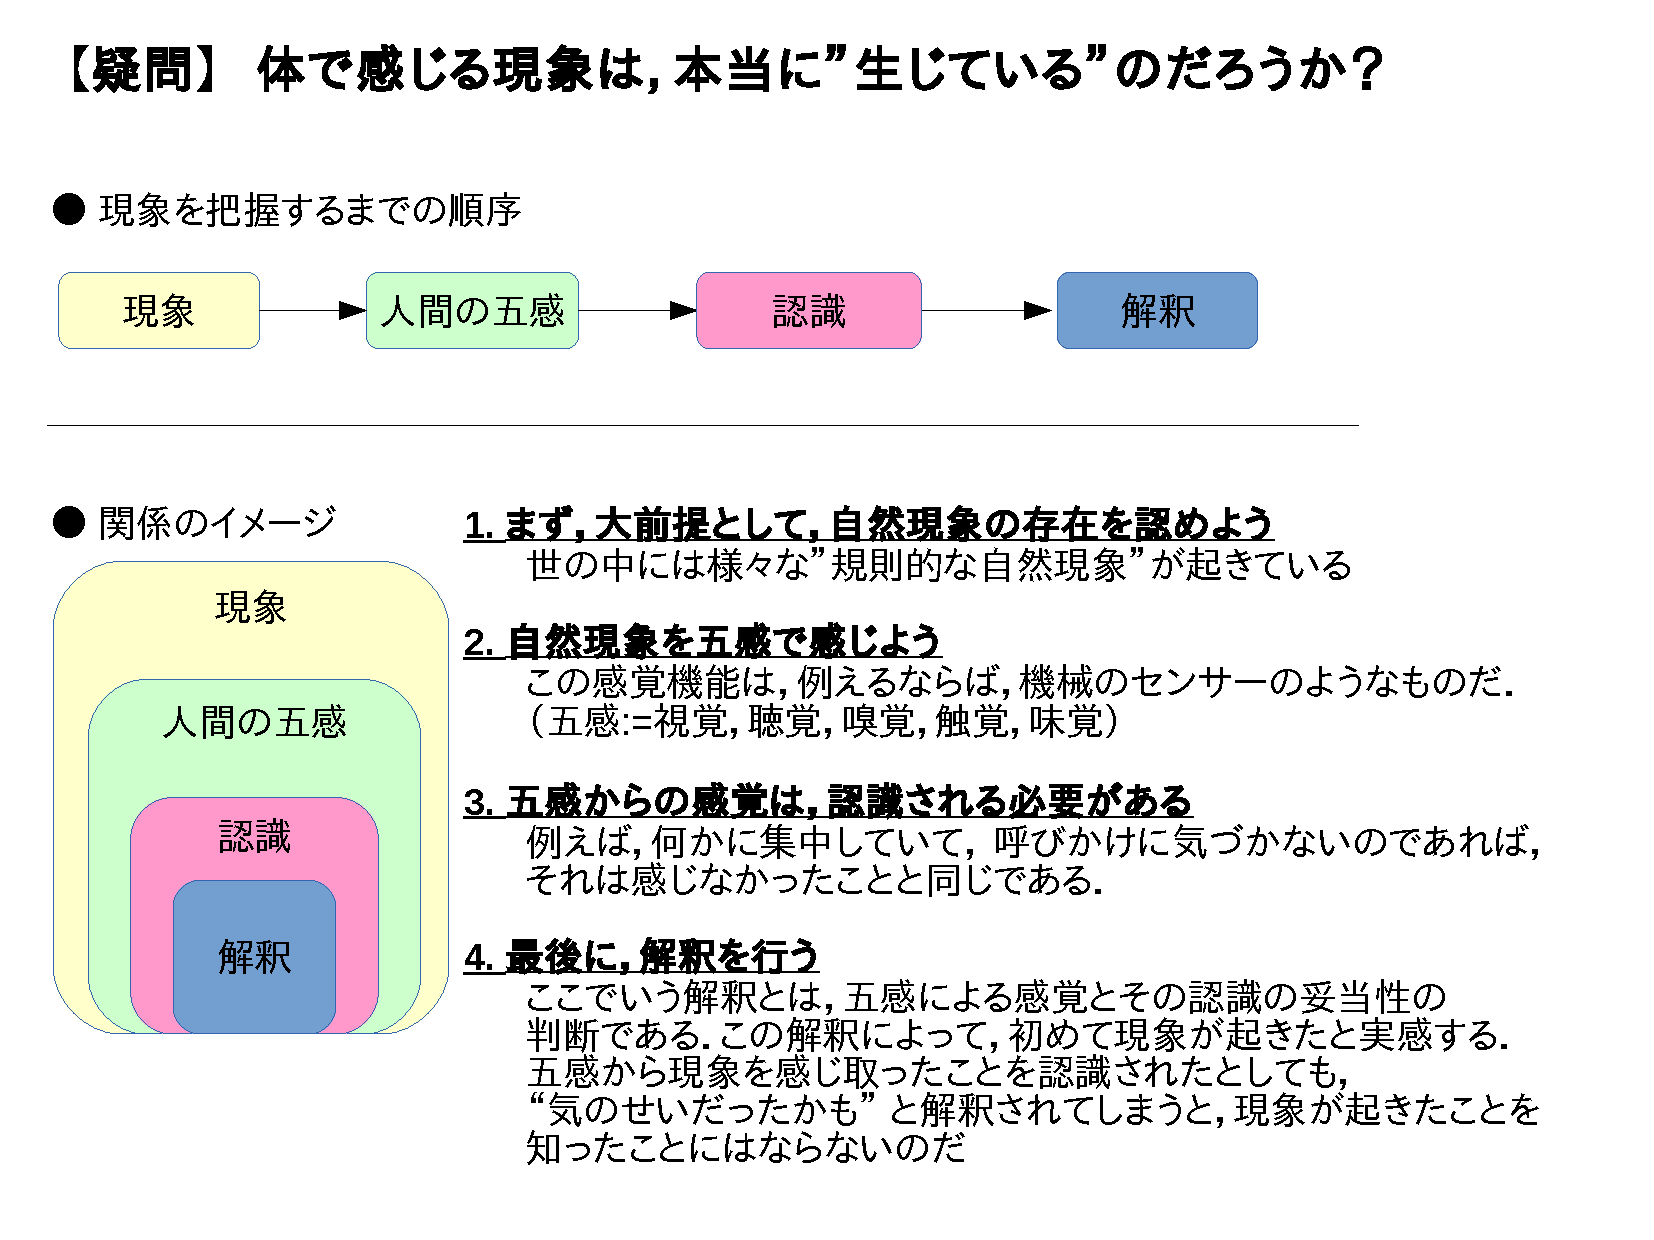
\includegraphics[keepaspectratio, width=7.2cm,height=6.35cm,clip]{kasetu.pdf}
                    \caption{科学的活動}
                    \label{fig:kasetu1}
                \end{center}
            \end{figure}

        \subsubsection{経験$=$現象を観察する}
            物理学は実験や経験を基に構成される.この経験というのは,私たちの五感
            で感じる経験のことである.この点で,経験を排除しようとする数学とは異る
                \footnote{
                    数学は,論理と算術のみによって,構成される.数学の構成には,
                    怪しげな経験などは含まれない.数学で仮定されるのは,ごく少数
                    の,それも誰もが正しいと認めるような,約束(\textbf{公理} と
                    呼ばれる)だけである.数学は,まず公理を構成し,その公理を満
                    たす対象の性質(\textbf{定理},\textbf{命題}など)を研究する.
                }.

        \subsubsection{仮説$=$現象の説明の試み}
            自然を肌で感じたことを,ノートに書き取る.いろいろ書いていくうちに,
            自然現象に共通点があることに気づく.そして,その共通点を元に,ある仮
            説をたてる.そして,その仮説を確かめるべく,実験をする.
            結果が正しければ,その仮説が立証させれたことになる
                \footnote{
                    仮説が否定さ
                    れる結果を得ることも多いが,仮説に対して肯定的な結果を得たときには,
                    さぞうれしいことだろう
                    こんな経験をしてみたい.
                }.

        \subsubsection{実験$=$仮説の検証}
            何度も言うが,実験により確かめるということが重要であり,これを怠っては
            ならない.物理学の基本的な作業工程は,
            経験を元に,仮説を立て,実験をしてその仮説の正しさを確かめることである.
            立てた仮説が多くの
                \footnote{
                    「多くの」というのは,"これまで知られている法則から導出される現象よりも,
                     多くの現象が説明できる" という意味で用いた.とい言うことは,
                     古い法則が新しい法則によって上書きされるのであるが,決して古い法則が
                     間違っていたとは解釈されない.それは,法則が "拡張された" と言い訳されるのだ.
                     このへんの考え方は,おそらく物理学の学習を進めていく段階で,自ずと,身についてしまう
                     ものだ.
                }
            自然現象を説明できるのであれば,それはいつしか「法則」と呼ばれるようになる.

            実験の大まかな手順は次の通りだ.まず,仮説を検証するために妥当な実験をしないとならない.
            仮説と全く関係のない実験をしても無意味だ
                \footnote{
                    体重を測ろうとしているのに,身長を測っても仕方ないだろう.
                }.
            そのためには,\textbf{実験計画} を立てる必要がある.適切な実験方法を考えるのだ.
            そして,実験器具を揃え,注意深く実験を遂行する.実験データはノートに書き残しておく
                \footnote{
                    個人的には,紙のノートにペンで記録したい.
                }.
            実験中の異変も記録しておくべきだ.
            実験が終わったら,結果を整理し,計画通りの実験が行えたかどうかを見直す.
            間違いがなければ,これで実験の終了である.後は考察するだけだ.

            実験から統計学や論理的推論により,実験で何が得られたかを考えることを \textbf{考察} という.
            実験が終わったら,必ず考察をして,実験による得られたことを明確にすべきだ
                \footnote{
                    考察を怠るということは,実験をしなかったことにするということである.
                    実験の目的は,仮説の妥当性を実証もしくは反証することである.
                    その判断を行うための前段階として,実験結果から何が言えるかを
                    考えないとならない,
                }.
            実験結果は,多くの場合,仮説の実証や反証よりもさらに深い知識を,私たちに提供する.
            考察をすることにより,実験結果から最大限の情報を引き出すのだ.

        \subsubsection{解釈(考察)$=$仮説の肯定,否定}
            さて,忘れがちなことだが,実験により得られたデータがその仮説を支持するか
            否かを判断することが必要である.このような行為を \textbf{解釈} という.
            仮説が物理法則になるための最後の関門が,この解釈である.
            多くの人々がその実験データが仮説を有力に支持すると判断したとき,
            その仮説は,法則と呼ばれるようになる.

            \subsection{自然現象の発生とその解釈}
            残念ながら,自然現象を人間が把握するには限界がある.
            いや,限界ではなく,制約という表現のほうがよいかもしれない.
            いずれにせよ,自然界で起こるすべての現象を正確に把握することは不可能
            である
                \footnote{
                    ここでは,立場を明確するために,不可能であると断言してしまったが,
                    実際のところ,こう断言するための根拠はない.主張を弱めて,
                    自然現象そのものを感じ取ることはできない,といったほうが
                    無難なのかもしれない.
                }.
            理由は,人間の五感
                \footnote{
                    「自然現象を感じ取るためのセンサー的機能」のことを指す.
                    人間が自然に対して直接的に干渉する部分は,この五感である.
                }
            と,その情報を処理する脳が絶対に正確であると言い切れないところにある.

            自然現象が発生したと人間が知る場合,まずそれは \textbf{五感} という感覚を
            通して通知される.
            そして,その感覚は脳へと渡り,初めて \textbf{認識} される.しかし,認識されるだけでは,
            まだ不安がある."気のせいだ" という判断したことがない人は,おそらく,いない
            はず.感覚を脳が認識したにもかかわらず,気のせいとしてしまい,片づけられたら,
            それは,認識されなかったことと同じである.自然現象が起きたことを確信する
            ためには,\textbf{解釈} することによる妥当性の保証が必要である.この解釈には,
            根拠ない自信であってもよいが,その現象を示す複数の感覚や証拠があるともっとよい.
            複数の人間が同じように認識したのであれば,それは有力であろう.とにかく,
            機能性ではなく,何かが絶対に起きたという解釈がなされることによって初めて,
            その現象がほんとに起こったこととして認識されるのである.

            現象を五感で感じ取り,それを脳で認識し,その妥当性を解釈によって判断することに
            よって,自然現象をとらえることができるのである.

            人間には,ウィルスを直接みることはできないし,
            超音波も聞こえず,紫外線も赤外線も見ることはできない.
            つまり,五感には限界があるということだ.
            先人はこれを克服すべく,顕微鏡を発明したり,現象を電圧や電流に変換するような
            装置を作ったりした.これによって,五感では感じ取れなかったことも"見える"ように
            なった.どうやら,五感に関する限界は,それにとってかわる装置を発明さえすれば,
            突破できるようだ.しかし,人間の思考(脳)については,今のところ,
            どんなに頑張っても,その正確性を保証することはできないようだ.

            "科学活動とは人間から見た自然現象の把握である"と考える
            人間原理的な立場では限界でも何でもないが,人間原理は
            新しい考え方を生まないために生産的ではなく,議論しても無駄だという結論しか導かれない.

        \begin{memo}{偶然と必然}
            科学では,偶然という考えは極力避けるべきである.
            自然現象は必然的に発生することであり,発生したすべての自然現象が総じて現実である.
            実際に発生していないことは必然的に発生していないのである.起きることも起きないことも
            必然であり,偶然ではない.

            しかし,必ず起きることとか,起きるかもしれないこととかの,判別の方法がない.
            偶然に起きたことだと思っていても,実はその発生は必然だったかもしれない.
            発生が必然的なものであったと思っていても,実はそれは偶然発生しただけかもしれない.

            例えば,ガラスのコップがテーブルから床へと落ちた場合を考えよう.
            仮に,コップが割れたとする.このとき,コップが割れたことは必然であろうか.
            一般的にガラスは落としたら割れるとされるので,コップが割れたことは必然であった
            とするのがしぜんであろう.しかし,もし,コップが割れなかった場合はどうか.
            コップが割れなかったことは,偶然であったと考えるのが妥当だと思うのだが,
            そう考えると,コップが割れることが必然であるという考えに矛盾する
                \footnote{
                    「落ちれば"必然"的に割れるガラスのコップが,"偶然"にもわれなかった」とは
                    どういうことか.偶然と必然は相反するものであり,
                    \textbf{必然的に起きることが偶然起きなかったなんてことは考えられない}.
                }.

            この矛盾を回避するために,可能性という概念を持ち出すことがある.
            コップが落ちたとき,コップが床に到達する直前では,コップが
            割れる場合と割れれない場合の2があるが,どちらになるかの判別は全くつかない.
            コップが床に衝突した後になってからそれがわかるのだが,割れるにせよ割れないにせよ,
            それは偶然的に起きたこととして認識される.つまり,可能性という概念を
            導入すると,現象の発生は偶然的であるということになる.だが,科学ではそうは考えない.
            床の硬度とコップの材料や形や強度とか落下速度などの必要な情報が全てそろえば,
            実際に落下しなくても,そのようなことが起きた場合を仮に想定して,割れるか割れないかの
            判別は計算によって判別することが可能であると信じるのである
                \footnote{
                    量子的な現象の場合には断定することができないのだが,
                    それでも統計的(確率的)にいうことはできる.
                }.
        \end{memo}

        \begin{memo}{相対主義と絶対主義/蓋然性の蓋然性}
            絶対に正しい真実はあるか.もしかしたら,あるかもしれない.でも,ないかもしれない.
            少なくとも,いままで見つかったことはない.答えは人それぞれであり,絶対的な答えはな
            いとする立場を \textbf{相対主義} という.他方,絶対に正しいという答えがあるとい
            う立場は \textbf{絶対主義} とよばれる.相対主義は正しいか,いや,もっと強く表現して,
            相対主義は絶対に正しいか.あれ,,相対主義が絶対に正しいとすると,絶対に正しいとする
            考えが存在するという立場にあるので,これは絶対主義である.矛盾だ.相対主義が正しいと
            主張する立場は絶対主義となる.ならば,相対主義も相対的に正しいのだと考えればどうか.
            だめだ.これでは,何も主張していないのに等しい.困った.これが相対主義のパラドクス.

            科学は仮設を実験的に検証することは可能だが,絶対に正しいとは言い切れない.
            そうかと言って,実験結果は人それぞれだというわけではないので,相対主義でもない.
            そうなると,「ある程度正しいだろう」という意味の \textbf{蓋然性} という考え方が浮上
            してくる.仮設が間違っているかもしれないという,譲歩的な気持ちがあらわれてくるのだ.
            でも,ちょっと待てよ.「『ある程度正しいだろう』という考え」はどの程度正しいのか.
            つまり,蓋然性という考え方の正しさはどの程度かI(蓋然性の蓋然性).正しさの根源を
            探ろうとすると,深みにハマる.答えが見つからない底なし沼だ.このあたりで,やめておこう.
        \end{memo}

        \begin{memo}{真偽と確実性}
            「Aであることは真実か」(真偽の問題)という質問と,「Aであることは確実か」(確実性の問題)という質問.
            両者は似ているようで異なる.真偽はあらかじめ決まっているものであり(我々が知らないだけ),実質的に根拠はいらない.
            他方で,確実性を考えるには根拠が必要である.「真であること」はありうるが,確実に真である保証はない.
            言葉と意味と論理に注意しておきたい.「『その事実が確実である』ことは確実ではない」といっているのではない.これは矛盾だ.

            例えば,未解決問題が解けたという主張があり,その主張が検証段階にある場合,
            その主張が真であるということは,確実ではない(いま,まさにこの検証をしているのだから).
            その主張が確実であるということは,真ではない(だからといって,確実でないことはない).
            確実性を問う場合には,確実ではない可能性が想定されている.真偽を問う場合には可能性は皆無である.

            真であることは真か,偽であることは真か,真であることは偽か,偽であることは偽か,真または偽であることは真か,
            同じ語彙を使う場合,メタレベルで考えないと矛盾に陥る.
            もっと,シックリくる説明はできないものか.
        \end{memo}


%       %======================================================================
%       %  SubSection
%       %======================================================================
        \subsection{論理的な飛躍}
            科学的な説明を聞いて,"もっともらしい"と感じたことはないだろうか.
            そして,それを論理的だと思ってしまったことはないだろうか.
            しかし,この感覚は間違っている.科学は論理的ではないのである.
            確かに,論証は論理的であるが,科学の根源的な法則は,論理的に導かれたものではない.
            先に説明したように,科学法則は経験や実験から推察することによって,
            得ているものであることを忘れてはいけない.この推察の部分に論理的飛躍があるのだ.

            \begin{memo}{例:ハッブルの法則}
                しばしば,仮説を表す命題の前提と結論を逆にすることにより一般化し,
                法則として捉えなおされることがある.

                具体的な例で考えてみよう.「ハッブルの法則」と言われている法則がある
                    \footnote{
                        ハッブル [著],戎崎 俊一 [訳],『銀河の世界』,岩波文庫
                    }.
                この法則が示すのは,宇宙が膨張していることである.その根拠は実験(観測)結果
                による.地球から見える天体が,遠ざかる速さとその距離が正比例する,というのが
                実験事実である.そして,そこから,宇宙が膨張していることが示されるという.
                論旨を追ってみると,まず,天体同士の距離が時間が経つごとに開くという観測事実
                がある.この現象は地球から見える宇宙のどの方向でも例外なく起こっていて,天体
                が近づくことはないという.つまり,宇宙のある所では天体間の距離が小さくなりつ
                つあり,別の所ではその距離が開きつつあるというのではなく,宇宙のいたるところ
                で,天体間の距離が同じように開いているというのである.宇宙の広がりに関する状
                態として考えられるのは3種類あり,
                (1)静止状態
                    \footnote{
                        広がったり縮まったりしておらずに定常状態を保っている,ということ.
                    },
                (2)広がりつつある状態,(3)縮まりつつある状態,である.
                この宇宙の3つの状態のうちでハッブルの法則に矛盾しないのは,(2)広がりつつある
                状態である.さらに,天体間には重力という引力が働いているので,天体同士が反発
                するということはありえない.つまり,宇宙は膨張していると結論できる,という.
                以上の論旨を整理しよう.
                    \begin{enumerate}
                        \item 天体間の距離は,宇宙の至る所で,広がりつつある(前提1$=$観測事実)
                        \item 天体同士は重力が働いていて,斥力はない(前提2$=$観測事実)
                        \item 宇宙が膨張しているとしないと,矛盾が生じる(論理的整合性の考慮)
                        \item だから,宇宙は膨張している(結論)
                    \end{enumerate}
                前提が実験事実である天体間の距離の拡大であり,結論が
                宇宙の膨張であるということに注意してほしい.ここまでは論理的な推論である.

                しかし,科学的解釈を加えると,ここから話が飛躍する.天体間の距離の拡大と宇宙
                の膨張を比べると,宇宙の膨張の方が根源的事実であり,天体間の距離の拡大は宇宙
                が膨張していることにより生じる1つの現象である,と考えるのが妥当だろう.要す
                るに,天体間の距離が広がりつつあるのは宇宙が膨張しているからである,という命
                題が立てられるのである.この命題は,さっきの論旨の逆である.以下のように記号
                化してみよう.
                \begin{description}
                    \item[A:] 天体間の距離は,宇宙の至る所で,広がりつつある
                    \item[B:] 宇宙は膨張している
                \end{description}
                法則を探り当てた段階では,A$\rightarrow$B だったが,一度宇宙の膨張が導かれる
                と,B$\rightarrow$A に置き換えられてしまった.論理的には,逆は必ずしも真には
                ならないのに.

                ここからは,B$\rightarrow$Aを法則として捉えてみよう.事実として現実に現れて
                いるのは,Aの天体間の距離の拡大である.そしてその根拠として,Bの宇宙の膨張が
                主張されている.しかし,この論理(B$\rightarrow$A)からは,AからBを導くことは
                できない.BはAを引き起こすことのできる1つの現象であると言えるが,それが唯一
                であるとは限らない.実際は何か別の現象Cがあって,C$\rightarrow$Aが成立してい
                ることも可能性として考えられるのだ.しかし,現在Cという可能性は提唱されてお
                らず,B$\rightarrow$Aの妥当性が極めて高いため,これを法則といっているのだ
                    \footnote{
                        論理的には,AとB$\rightarrow$Aが与えられた場合,"Bの可能性がある" としか
                        言えない.AとB$\rightarrow$Aから.これを科学法則に仕立てあげるには,
                        B以外の原因Cが起こり得ない(現実的に考えにくい/起こりにくい)ことを
                        示さなければならない.
                    }.

                科学的推論は論理的ではない.頻繁に使われる帰納的推論やアブダクションは必ずしも正しい結論に到達
                するわけではない.また,意図的に前件否定,後件肯定などが行われる.だから,科学には実験的検証と
                いう作業が欠かせない.科学には実験がつきものである理由がここにある.そして数学との違いも,ここ
                にある.

                数学的推論は,人間のうっかりミスなどがない限り,必ず正しい結論に到達する.ABC予想」,
                「リーマン予想」など予想があるが,これらは証明されていないので,「予想」とされている.
                科学であれば,現状観測し得るすべての場合で,その予想に反する事実がなければ,「正しい」
                とされる.しかし,数学は論理的推論によりその結論に達しない限りは,正しいとみなされない
                    \footnote{
                        数学は科学ではない.数学は科学の最重要な道具であるが,科学ではない.数学の方が
                        論理的に厳密である.数学は現実を反映しない.現実を離れて抽象化される.現に,物
                        理学的には,この世界は空間3次元と時間1次元の世界であるが,数学では次元は無限に
                        さえなり得る,科学は世界に忠実であろうとするが推論や論理に穴がある.数学は誤り
                        はないが,必ずしも現実世界に忠実であるとは限らない(現実を離れた抽象化できる).
                    }.
            \end{memo}

%       %======================================================================
%       %  SubSection
%       %======================================================================
        \subsection{推論の種類}
            科学は,実際の現象を感じ,その規則性を推論し,仮説を立てて,実験により
            その仮説を検証してその正しさを確かめることで,知識を増やしていく.
            その過程で行われる推論は大きく分けて3つある.ここで,推論という行為
            について,少し考えておこう.一言で推論といっても,その方法はいくつも
            ある.しかし,共通して言えることは,すでに得られている知識から,新しい
            知識を導き出すことである.その方法は,
            \textbf{演繹的推論},\textbf{帰納的推論},\textbf{発展的推論} がある.

%           %==================================================================
%           %  SubsubSection
%           %==================================================================
            \subsubsection{演繹的推論}
            演繹的推論は,例えば,数学の定理証明で使われる推論であり,三段論法を
            駆使して行われる行為である.この演繹的推論では常に正しい結論を得ることが
            できる
                \footnote{
                    もちろん,ケアレスミスなどの,人的な誤りがなければ,という
                    ことだ.人的な誤りはミスは必ず見つけれる.
                }.

%           %==================================================================
%           %  SubsubSection
%           %==================================================================
            \subsubsection{帰納的推論}
            帰納的推論とは,いくつかの現象から共通な部分を抜き出し,
            法則性を導き出す行為である.例えば,ケプラーの天体の運動に関する3つの法則
            は,帰納的推論により導き出されたものである.膨大な天体観測記録から,
            天体の運動の仕方に規則性を見出したのである.

%           %==================================================================
%           %  SubsubSection
%           %==================================================================
            \subsubsection{発想的推論}
            発想的推論とは,過去の経験や知識を基に,因果関係を探る行為である.
            例えば,ニュートンが発見した万有引力は,発想的推論により導き出された
            ものである.手で持った物体を,ある高さから静かに手を放すと,地面に
            落ちる,という現象が目の前で起こっているとする.物体が落ちるという現象は
            見ることができる明らかな事実であるが,その落ちる原因は直感的にはわからない.
            なので,推論によってその原因を探る必要がある.ものが落ちるという現象を引き起こす,
            もっともらしい原因を見つけ出す行為こそが,発想的推論なのだ.形式的に言えば,
            現象Xが知られていて,その原因として,仮説Yが成立していれば,現象Xが起こること
            が必然だとすると
                \footnote{
                    今までの例で言うと,X:物体の落下,Y:万有引力の法則 となる.
                },
            仮説Yが成立しているという結論が有力に支持される.もちろん,現象Xを
            説明できるのは,複数の仮説が考えられるはずである.この複数の仮説から
            真の原因を選び出すためには,実験と推論を繰り返す必要がある.
            発想的推論を短くいうならば,"Xであるという事実" を目にしたとき,
            "YならばXであるという必然的因果関係" があるならば,"Yかもしれない" という
            結論を得る推論ということになる.

%           %==================================================================
%           %  SubsubSection
%           %==================================================================
            \subsubsection{科学的推論}
            \begin{mysmallsec}{長所と短所}
            帰納的推論と発想的推論の長所は,新しい知識を生み出すことができるところだ.
            欠点は,人の経験や思いつきなどが絡みあい,
            間違った結論を導き出すという危険な副作用があるということ.
            更に欠点をいうと,これらの推論で得た結論は,将来起きる未知なる現象により,
            覆される可能性があるということだ.実際に起きていないことや過去に経験のないことに対しては,
            何も手が出せないのである.

            これに対し,演繹的推論は常に正しい結論を導くことはできるが,
            新しい知識を作り出すことはできない.しかしその代わりに,一度導き出された
            知識は,未来永劫にわたって真であり,覆される可能性は全くない.
            \end{mysmallsec}

            \begin{mysmallsec}{科学的推論}
            科学と数学と違いは,帰納的推論と発想的推論にある.
            これらの推論には間違いが含まれるかもしれないというリスクはあるが,
            それを補ってあまりある新しい知識を創造できるのである.
            対して,数学は演繹的推論のみを採用しており,帰納的推論と発想的推論は
            禁止されている.それが故に,数学はいつなん時でも正しい結論が得られる.

            科学的推論とは,帰納的推論や発想的推論で得られた知識を,
            演繹的推論によって洗練させて,実際に起来ている(あるはこれから起きるだろう)
            現象に対する有力な説明を与えることである.
            \end{mysmallsec}

%       %======================================================================
%       %  SubSection
%       %======================================================================
        \subsection{再現性}
            経験より得られた仮説は,実験を行って,その正しさを確かめないといけな
            い.けれど,全ての仮説に対して,実験が行えるわけではない.実験不可能
            な仮説も存在するのである.

            実験不可能な仮説の有名な例として,「幽霊の存在」がある.なぜ,幽霊の
            存在を実験的に確かめることができないのだろうか.ここには,実験の再現
            性がかかわっている.

            実験に要求されることのひとつとして,再現性がある.\textbf{再現性} と
            は,同じ環境で同じように実験を行うと,同じ結果を得ることだ.全く同じ
            条件で,全く同じ方法で実験を何回か行って,それぞれで異なった結果を得
            るのでは意味がない.もし,毎回結果が異なるのであれば,検証すべき
            その仮説は間違いであったと結論されるか,実験が正しく行われなかったか,
            原因は様々であるが,いずれにしても,何も得られなかったことになる.

            幽霊の存在の話に戻ろう.幽霊が存在することを実証できないのも,
            再現性のある実験方法がわからないからである.突如として現れる幽霊は,
            その発生条件すらもわからず,おまけに,目で見えたり見えなかったりする.
            心霊写真といわれるものがあるらしいが,それも幽霊の存在の実証にはなら
            ない.こうすれば絶対に幽霊の写る写真が取れる,という方法が確立されれ
            ばよいが,成功例はなく,難しいようである.

            再現性が要求されるのは,誰でも確かめられるということが重要だからであ
            る.客観的に自然現象を捉えるには,再現性は非常に重要な要請である.

            実をいうと,現在の物理学の実験は多くの場合非常に難しい実験であり,何
            度でも誰でも気軽に行えるものではない.それでは再現性があるとはいえな
            いのではないか,と考えてしまうかもしれないが,物理学者は再現性をもっ
            と緩くとらえているようである.すなわち,物理学者は,再現性がある実験
            かどうかを判断し,再現性があるだろうことが認められれば,それで良し
            とするのである.このことについて,中谷宇吉郎
                \footnote{
                    中谷宇吉郎(1900--1962, 日本):物理学者.雪についての研究が
                    一般的に有名.「雪は天から送られた手紙である」という有名な文
                    句でも知られる.
                }
            の易しい説明があるので,これを次に引用しておこう.
                \begin{memo}{「科学の方法」(中谷宇吉郎:岩波新書)より}
                    科学について,何かを論じようとする場合に,まず取り上げるべき
                    問題は,科学の限界の問題である.今日われわれが科学と称してい
                    るものは,その取り扱い得る問題,限界があるか否かというを,ま
                    ず検討してみる必要がある.

                    今世紀(20 世紀) に入って,科学が非常に進歩し,特に自然科学が
                    最近になって,急激な発展をとげたことは,いまさら言うまでも
                    ない.いわゆる,人工頭脳のような機械ができたり,原子力が解放
                    されたり,人工衛星が飛んだりしたために,まさに科学ブームの世
                    の中になった観がある.そしてこの調子で科学が進歩を続けていく
                    と,近い将来に人間のあらゆる問題が,科学によって解決されるで
                    あろう,という異様な錯覚に陥る人が,かなりあるように思われる.

                    もちろん科学は,非常に力強いものではあるが,科学が力強いとい
                    うことは,ある限界の中での話であって,その限界の外では,案外
                    無力なものであることを,つい忘れがちになっている.いわゆる,
                    科学万能的なものの考え方が,この頃の風潮になっているが,それ
                    には,科学の成果に幻惑されている点が,かなりあるように思われ
                    る.これは何も人生問題というような高尚な話ではなく,自然現象
                    においても,必ずしも全ての問題が,科学で解決できるとは限らな
                    いのである.今日の科学の進歩は,いろいろな自然現象の中から,
                    今日の科学に適した問題を抜き出して,それを解決していると見た
                    ほうが妥当である.もっとくわしくいえば,現代の科学の方法が,
                    その実態を調べるのに非常に有効であるもの,すなわち自然現象の
                    中のそういう特殊な面が,科学によって開発されているのである.

                    それはどういう面かというに,まず第一に,一番重要な点をあげれ
                    ば,科学は再現可能な問題,英語でリプロデューシブルといわれて
                    いる問題が,その対象となっている.もう一度繰り返して,やって
                    みることができるという,そういう問題についてのみ,科学は成り
                    立つものである.

                    なぜ再現可能の問題だけしか,科学は取り扱い得ないかといえば,
                    科学というものは,あることをいう場合に,それがほんとうか,ほ
                    んとうでないかということをいう学問である.それが美しいとか,
                    善いとか悪いとかということは,決していわないし,またいうこと
                    もできないものである.

                    それでは科学で,ほんとうであるというのは,どういうことかとい
                    うことを,まず考えてみる必要がある.ごく簡単な場合についてい
                    えば,いろいろな人間が同じことを調べてみて,それがいつでも同
                    じ結果になる場合には,それをほんとうというのである.最も
                    同じことを同じ方法で調べることができない場合もある.しかし人
                    間が自然界を見るときには,いつでも人間の感覚を通じてみるわけ
                    だが,この感覚を通じて自然界を見ることによって,ある知識を得
                    る.その得た知識と,他の人がその人の感覚を通じて得た知識と
                    の間に,互いに矛盾が無い場合には,われわれはそれをほんとうで
                    あるという.そうでない場合には,それはまちがっているというわ
                    けである.

                    (中谷宇吉郎[著],『科学の方法』,岩波書店(岩波新書),1998 より
                    \footnote{
                        初版は1958年.
                    }.)
                \end{memo}


%       %======================================================================
%       %  SubSection
%       %======================================================================
        \subsection{単純性:オッカムの剃刀}
            理論はできるだけ複雑にならないように組み立てるべきだ.
            この考え方を,\textbf{オッカムの剃刀} という
                \footnote{
                    William of Ockham(13世紀後半--14世紀前半,イギリス):
                    英語表記をそのまま訳すと,「オッカムのウィリアム」となる.
                    「オッカム」というのは,当時のイギリスの地名.
                    ウィリアムという名前でなく,地名であるオッカム
                    のみがその表現に残っているのかは不明.
                }.
            何かを説明するのに,必要以上の仮定を避けるべきだ,という考え方
            である.必要以上の仮定が含まれている理論を,カミソリによってそぎ落とし,
            より単純化するイメージ.

            但し,初めて人に説明するときは,これを正直に実行してしまうと,
            簡潔すぎて正しく伝わらないことだろう.
            概念をわかりやすく説明するためには,初めは多少遠回りをして,物事を考えるこ
            とも必要である.その場合,概念を理解した後に,単純性を満たすよう
            に整理すればよい.

            そうかといって,最も単純な理論がどのようなものなのかはわかりよう
            もない.単純さという感覚はどうにも曖昧だからだ.つまり,これには
            答えがない.「おぉ,単純だ.美しい!!」という直感が大事だ.

            もちろん,最初からできるはずもない.最初は何もわかっていないのだ
            から,論理的に不完全な推論しかできない.しかし,その推論がどうも
            正しい方向にあると感じたら,その足りない部分を補って,理論を構成
            していく.理論を構成していく上で,それまでに必要だと思っていたこ
            とが,実際には無駄なことであったというような部分も,見つかるかも
            しれない.そうした無駄な部分は削除される.こうして,単純な理論が
            構築されていく.時間をかけて無駄な部分を省き,シンプルにしていく
            のだ.

            単純性を追求してしまうと,それと同時に,「理論を作り上げるまでの
            考え方」も,削除されてしまう.どのようにして,その理論を作り上げ
            たのかが,わからなくなってしまうのである.いま学習している物理学
            は,既に単純化された理論である.この単純化された理論は,初めて物
            理学を学習する場合,とてもとっつきにくいものになっているだろう.
            なぜなら,単純な理論を構築するときに,その構築方法までも削除され
            ているからだ.理論を受け入れる場合は,単純な理論ではなく,理論に
            無駄部分はあっても,受け入れやすい形であることも大事である.理論
            の受け入れ方として,まず無駄な部分を含むが受け入れやすい形で,そ
            れを理解し,その後に単純化された理論を再度学ぶという方法がよい.

            ちなみに,このように,できるだけ理論を単純化しようとする動き
            を \textbf{思考経済} とよんだりする
                \footnote{
                    オッカムの剃刀と同じことを主張する,別の言い方.
                    いろんな言われ方があるくらいに,重要な考え方なのだ.

                    Everything should be made as simple as possible, but not simpler.
                    (A. アインシュタイン)
                }.
            できるだけシンプルに考える
            という思考方法である.思考経済は物理学に限ったことでなく,学問
            であるならば必ず採用されて いる.学問体系を構成する理論が冗長で
            あっては格好が悪いし,できる だけシンプルにまとまっていた方がわ
            かりやすいのだから.

            \begin{memo}{「オッカムの剃刀」は正しいのか}
                オッカムの剃刀は全面的に正しいとは限らない.
                単純な理論ほど良い理論であると,必ずしも言えないのだ.
                最も単純な理論は,神を持ち出すことである.
                どんな複雑な現象でも,神を理由にすれば,その説明はとても単純になる.
                少なくとも,いま知られている
                物理法則から現象を説明するよりは単純になる.しかし,これでは本末転倒だ.
                物理学の目標は,神を持ちださないで物理現象を説明することなのだから.
                つまり,オッカムの剃刀という考え方にも,適用限界があるということだ.
                どこに限界があるかを考えるべきだが,簡単には答えは見つかりそうもない.
                とても難しい.

                ここでは,オッカムの剃刀と言う考え方は不完全であることを
                気に留めておくことにし,難しい議論は避けよう.
            \end{memo}


%       %======================================================================
%       %  SubSection
%       %======================================================================
        \subsection{客観と主観}
%           %==================================================================
%           %  SubsubSection
%           %==================================================================
            \subsubsection{客観性}
                物理は客観的であるべきだ.しかし,物理学は本当に客観的に構成されているのだろうか.
                物理学に要求される客観性とは,どういったものなのだろうか.
                ここで,少し考えてみたい.

                世の中に存在するヒトの人数は,数十億人と
                言われる.物理で扱われる事柄は,これら数十億人のヒトにとって,
                共通でなければならない.言い換えれば,解釈がヒトによって異なってはならない.
                この客観性が,物理に課せられた条件の1つである.

                しかし,実際のところ,物理学を少し学習していくと,あるいは,
                物理学の啓蒙書を読みあさってみると,物理の解釈が人それぞれで異なって
                いるように,感じられる
                    \footnote{
                        「物理の」と曖昧に書いている.具体的には,「物理法則の」と
                        読み替えてもらえると,話が通じるはず.
                    }.
                つまり,物理は,完全には客観的では
                ないということである.おそらくこれは,物理が経験に基づいていることにあると思う.

                物理は数学とは違い,人間の経験を基に
                理論構築される.その理論の正しさの確認も,実験という経験を
                通してなされるものである.もちろん,経験といっても,一人の人間しか
                経験できないようなものではなく,すべての人ができる経験である.

                物理学に課せられている客観性とは,全ての人が経験できる事柄である.
                そして,その経験はすべての人に共通でないといけない.しかし,経験は
                人間ひとりひとりが感じるものであり,その感じ方(解釈)は人によって
                ことなる.だから,物理学ではこのような解釈の違いを排除すべく,
                基本単位を定義することにより,客観性を作り上げている.
                例えば,温度などは,"熱い"や"冷たい"などと表現するのではなく,
                セ氏何度という表現をしている.温度計を用いて,温度を測定する事により,
                熱いや冷たいなどと表現するのではなく,「セ氏20度」などと,万人に
                共通であるようにしているのだ.これにより,温度が客観的に表現された
                ということになる.

                もう少し,温度の例を考え続けよう.よく考えてみると,客観的に表された
                と思った温度であるが,本当に客観的なのだろうか.ここでいう「客観的」という
                語彙の意味は,すべての人にとって,同じであるという意味である.
                つまり,「セ氏20度」はすべての人に共通なのだろうか.共通であれば,
                客観的であるといえよう.しかし,それを知る術はないし,さらに言えば,そうではありえない.
                なぜなら "「セ氏20度」はすべての人に共通" ということは,「セ氏20度」という温度を
                経験する全ての人が,全く同じように暖かさを感じるということになるからである.
                これは,今までの私達の経験に反している.北海道などの北部に住む人々にとって,
                セ氏20度は,暖かく感じられ,沖縄などの南部の地方に住む人々にとっては,涼しく
                感じられるのではないか.更に言うと,一人の人間でも,季節の違いにより,温度の
                感じられれ方はことなる.夏のセ氏20度は涼しく感じられるし
                    \footnote{
                        むしろ寒いくらいだ.
                    },
                冬であれば暖かく感じる.セ氏温度により,客観的に温度を表現はできるものの,
                温度を感じるのは人間であり,つまり,そこに主観が入り込んできて,客観性が
                失われる.では,「セ氏温度の導入が,物理に客観性を生むのに失敗しているのだろうか」といえば,
                それは違う.現に,温度計を用いて温度を測ることには,客観性があることは,
                明らかである.いつでもどこでも,セ氏20度が変わることはない.

                ここに,温度の客観性に関して,矛盾が感じられる.大げさに言えば,
                宇宙のどこで測っても,セシ温度は共通であり,つまり,温度が客観的に
                表現されている.一方で,温度とは,人間が感じるものであり,その感じ方は,
                人それぞれ違うものであり,また,時期によってもその感じられ方は異なるので,
                客観性がないように思われる.どこが間違っているのだろうか.答えは簡単で,
                人それぞれの感じる温度を客観的に示すべくセ氏温度が導入されたのだから,
                温度を感じる人間を持ち出したことが,間違いであったのだ.要するに,人間の体験
                の排除をすることにより,客観性を産み出しているのである.セ氏20度の
                感じ方は,人それぞれ違うのは当たり前.それを統一すべくセ氏温度が導入されたのだ.

                別の例を上げてみよう.色に関する経験を考えてみる.「青」という色は,
                全ての人間に全く同じように感じられるのだろうか.答えはあからかにNoである.
                「青」という色を感じ取るのは,人であり,個体差があって当然である
                    \footnote{
                        目の作り,目で感じた光を脳に伝える神経の作り,脳の作りなど,
                        色を感じるための機構が同じである二人以上の人間がいるとは考えにくい.
                        色の感じ方は,人によって違うと考えたほうが自然である.
                        まあ,人によって同じかどうかということを考えることそのものが,
                        無意味である.なぜなら,確認のしようがないのだから.
                    }.
                では,物理では色を客観的に示すことはできないのだろうか.もちろん,そんなことはない.
                色は光であり,光は電磁波という波の一種であることがわかっている.物理で言う色の違い
                とは,この波の波長
                    \footnote{
                        周波数といっても同じことだ.$\nu T = 1$ ($\nu$ は波の周波数,$T$ は波の周期) の
                        関係式が成立しているはずである.周波数とは,一秒間で振動する波の回数であり,
                        周期とは,一回の振動にかかる時間のことである.つまり,$T = 1/\nu$ が成り立つ.
                        一秒間に $\nu$ 回振動するのだから,1を $\nu$ で割ることにより,周期を計算できる.
                    }
                の違いである.色を波長という数値で定義することができ,これにより,人間の
                体験の排除が実現されるのである.色を感じるのは確かに人間であるが,色を客観的に
                表現するには,人間の経験を排除しなければならない.その代わりに,番人に共通である
                波の波長という数値を導入するのである.

                長々と書いてしまったが,話を元に戻そう.何が言いたかったかというと,
                物理学における客観性とは何かということである.その答えは,もう既に
                書いてしまったが,\textbf{人間の体験の排除}である.数値は万人にたいして
                客観的事実を伝えるのであるから,人間の体験を数値で置き換えることをすることにより,
                客観性を保とうとしているのである.

%           %==================================================================
%           %  SubsubSection
%           %==================================================================
            \subsubsection{"客観" と "主観" の違い}
                物理,あるいはもっと範囲を広げて,科学とは客観的に構成される.
                しかし,客観的な科学はそのままでは,使いものにはならない
                    \footnote{
                        物理法則の理論的な側面だけを追求しようとする人には,
                        それで十分だと思われるかもしれないが,それにしても,
                        その物理法則の捉え方は人それぞれ解釈が異なる.
                        (式の解釈が万人に共通であるとは考えにくい.法則を表す式は一般的に
                        表現されるものであり,完全に意味付けされていない.具体的に意味づけしようと
                        する際に,解釈の違いが生まれてくる.これから,学習するニュートンの法則
                        もそれに同じ.図書館などで多くの教科書を探ってみよう.様々な説明のされ方が
                        なされることを知るだろう.)
                    }.
                科学は解釈しなければ,使うことができない.解釈するということは,そこに
                解釈者の主観が交じるということである.
                この解釈するという行為は,勘違いしやすく,矛盾に陥りやすい
                ところなので,特に注意しないといけない.

                科学を解釈するということは,客観的に記述されている科学的事実を解釈するという
                ことであり,科学が客観的でなくなるわけではない.

                科学の理論構築は,始めは人間の経験や体験によるものであるが,それを
                数値化することで,客観性をつくり出している.科学理論は客観的
                である.それを解釈するのは人間であり,この時に科学の客観性が失われ,主観が生じる.

                科学のおける客観性と,その解釈により生じる主観性は区別して考えなければならない.

%           \begin{memo}{「数」と「量」}
%               モノの個数を数えることを考えよう.具体的に考えるため,モノの例に果物をとる.
%               目の前に,林檎,蜜柑,苺,葡萄,桃がそれぞれ置かれているとしよう
%               (図\ref{fig:kudamono})
%                   \footnote{
%                       とりあえず,5種類を上げたが,この説明で使用するのは林檎と蜜柑
%                       だけ.他の果物は特に意味のないもの.果物がたくさんあったほうが,
%                       見栄えがいいでしょ?
%                   }.
%                   \begin{figure}[hbt]
%                       \begin{center}
%                           \includegraphicsdouble{kudamono.pdf}
%                           \caption{目の前に,美味しそうな果物が!}
%                           \label{fig:kudamono}
%                       \end{center}
%                   \end{figure}
%
%               それぞれの果物の個数は,見るからに異なる.では,どれだけ違うのか.
%               直接示して,林檎は
%                   \begin{figure}[hbt]
%                       \begin{center}
%                           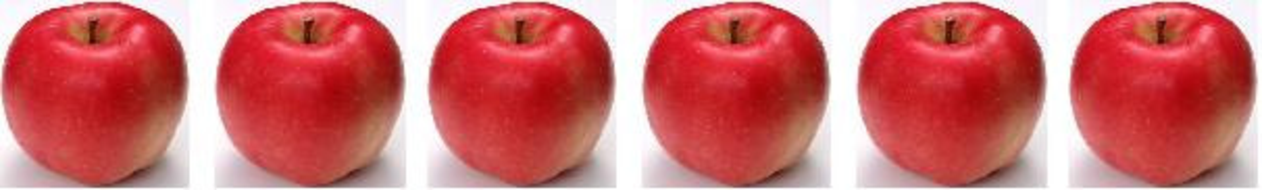
\includegraphics[keepaspectratio, width=3cm,height=0.5cm,clip]{kudamono_apple.pdf}
%                           \label{fig:kudamono_apple}
%                       \end{center}
%                   \end{figure}
%               であり,蜜柑は
%                   \begin{figure}[hbt]
%                       \begin{center}
%                           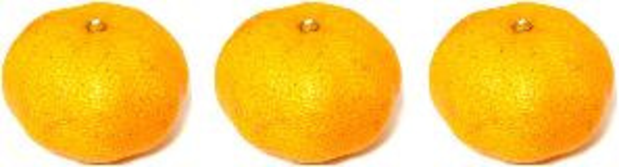
\includegraphics[keepaspectratio, width=1.5cm,height=0.4cm,clip]{kudamono_orange.pdf}
%                           \label{fig:kudamono_orange}
%                       \end{center}
%                   \end{figure}
%               だ,といったところで,具体的な個数の違いを示せない.
%
%               ここで,\textbf{数} という概念が有用になる.\textbf{一対一対応} という考え方を使うのだ.
%                   \begin{figure}[hbt]
%                       \begin{center}
%                           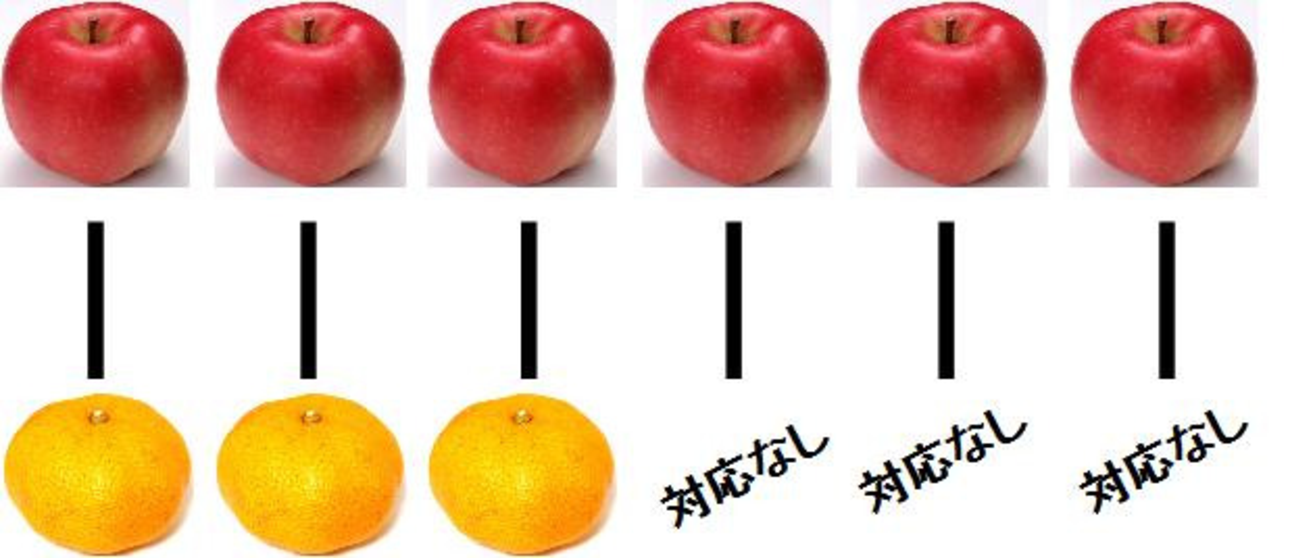
\includegraphics[keepaspectratio, width=4cm,height=1.8cm,clip]{kudamono_comp.pdf}
%                           \label{fig:kudamono_comp}
%                       \end{center}
%                   \end{figure}
%           \end{memo}

%       %======================================================================
%       %  SubSection
%       %======================================================================
        \subsection{法則}
%           %==================================================================
%           %  SubsubSection
%           %==================================================================
            \subsubsection{還元主義}
            科学は \textbf{還元主義} という思想が強く反映されている.
            還元主義とは,どんなに複雑に見える現象でも,それらを詳細に分析
            することで,複数の簡単な問題に捉えなおすことができる,という
            考え方だ.

            物理学の目的の1つに,「少数の規則を議論の出発点として,現実に起こっている
            現象を説明すること」というものがある.しかし,実際の全ての現象が,
            少数の規則
                \footnote{
                    少数の規則:"少数"と曖昧に表現したのは,
                    個数には特にこだわらないからである.
                    しかし,規則の個数は有限個である必要があることを要求する.
                }
            で説明できるという保証はない.人がそう信じているだけだ.
            しかし実際のところ,この考え方によって物理学は発展している.
            もちろん,説明できない現象も多いが,それらについても,
            将来の物理学の発展によって,説明可能であるとされている.
            要するに,何の根拠もない考え方だけど,今までこの考え方で成功してきているのだ.

            還元主義は,今まで大成功を収めているので,根拠がないという理由で捨てることは
            できない(もったいない).足元が不安定に感じるかもしれないが,
            信じるしかないようだ.

            \begin{memo}{科学的思想の根本?}
                還元主義に根拠がないなど,科学の思想的土台はとても不安定だ.
                そもそも経験に根拠があるはずがなく,それ基にした学問だから仕方ない.
                科学とは,多くの人間の様々な経験の中から,"いつもそうなる" というものを抜き出して,
                それらを整理して体系立てることである
                    \footnote{
                        いろんなところで,"科学とは" といった説明を聞くだろう.
                        実際,このノートでも複数の箇所に,そういった表現がある.
                        しかし,そこで表現されていることが唯一ではなく,
                        科学という活動にはそういった一面もある,ということを言いたい.
                    }.
                科学に対して,論理学や数学のような強い理論的土台を求めてはならない.
                間違いに気が付いたら見直す,というくらいの気構えが必要だ.

                こう言ってしまうと,「科学的に立証された」という表現に対して,
                少々不信感が出てきてしまうかもしれない.それは正しい.科学には
                潜在的な間違いが含まれていることを,承知しておくべきだ.
                しかし,だからと言って,科学を過渡に拒否するのはもったいない.
                先人の多くの経験や実験による成果によって,現在の科学技術を駆使した
                生活があることも事実である.

                科学は間違っている部分もあるけれど,だからと言って,それを捨てるのは
                得策ではない.もし,間違っているかもしれないと感じた部分があれば,
                それを確かめるための実験を繰り返し行うことで,信頼性を高めることが
                可能だ.科学を安易に信頼するのも,過渡に拒絶するのもよくない.
                科学の性質を理解して,適切な認識をもつことが理想である.
            \end{memo}

%           %==================================================================
%           %  SubsubSection
%           %==================================================================
            \subsubsection{規則性の発見}
            実験や経験を基にして物理学を構成するには,まず,それらを言葉で表現す
            る必要がある.例えば,「落とした消しゴムは,拾わないと机には戻らな
            い」とか,「破れた紙は,元の状態に戻すことはできない」とかといった
            具合に.ときには,数式で表現されることもある
                \footnote{
                    数式によって表現されても,その根底には,言葉による表現がある.
                    言い換えれば,言葉による表現を数式として表すということだ.物
                    理は記号の羅列ではない.あくまでも,肌で感じた経験と,実験で得
                    た知識を前提にして,物理学は構成される.
                }.

            いろいろと,経験・実験を繰り替えしていき,それを言葉によって書き留め
            る.多くを経験したり,多くの実験を行えば,書き留められる言葉もそれだ
            け多くなる.このたくさんの言葉による経験・実験の記述を読み返し,吟味
            してみると,何かそれらの間で共通する部分を見出すことになる.

            例えば,「『鉛筆』は机の上から床に落ちる.拾わないと机の上には戻らな
            い」と言う記述と,「『教科書』は机の上から床に落ちる.拾わないと机の
            上には戻らない」という記述があったとしよう.鉛筆だろうが教科書だろう
            が,落ちたものは拾わないと元の位置には戻らない.当たり前のことだが,
            このことに気づくことが大事である.これが「法則」を得る第一歩だからで
            ある.

            ニュートン
                \footnote{
                    Sir Isaac Newton(1643--1727, イギリス):物理学の創始者.ケ
                    プラー(Johannes Kepler, 1571--1630, ドイツ)が唱えた「天体の
                    運動の3つの法則」を含む,物体の運動に関する3つの法則を提唱し
                    た.天体の運動と,地上ある「もの」の運動を同一視(同じように
                    見るということ)し,力学(「ニュートン力学」)を作り上げたの
                    である.「Philosophiae Naturalis Principia Mathematica」(和
                    訳名:自然哲学の数学的諸原理,もしくは,プリンキピア)によっ
                    て,現在に伝わっている.この過程で,微積分学を生み出した.数
                    学においても大きな貢献があるのだ.二項定理の証明も行っている.
                    また,物理学の他の貢献として,冷却の法則や光学に関する考察も
                    有名である.
                }
            は,たった3つの記述によって,どんな「もの」運動でも記述できることを示
            した.このような3つの記述のことを \textbf{法則} という.法則とは,ど
            んな「もの」でも,もっている性質である.

            規則を発見したところで,これからもその規則が成り立つという保証はどこにも
            ない.これを補うためには,反例を立証できないとあきらめの雰囲気が出るくらい,
            何回も実験を繰り返すことしかできない.

%           %==================================================================
%           %  SubsubSection
%           %==================================================================
            \subsubsection{法則は理論の土台である}
            物理学にはいくつかの \textbf{法則} がある.法則とは,実験によって確認される現象である.
            法則は論理的に説明されるものでもなければ,他の概念から定義されるものでもない.
            法則は理論の最も基本的な土台であり,実験のみによって実証されるべき仮説である.
            「なぜ法則が成り立つのか」を考えること は大事なことだが,それはとても難しい問題
                \footnote{
                    「難しい問題」とは,「解くのにものすごく時間がかかる」という意味であり,
                    「解けない問題」や「答えのない問題」とは異なる.そもそも,解法や答えがない問題は,
                    もはや問題ではなくなる.
                }
            であって,そう簡単には答えは出せない.

%           %==================================================================
%           %  SubsubSection
%           %==================================================================
            \subsubsection{法則の正しさ}
            法則は実験によって確認されるべきことである.だから,実験の \textbf{誤差} が
            その法則の1つの限界条件を与えている.例えば,光速を測るにしても,無限大桁の数値を
            測することは実際上において不可能であり,従って人間の知り得る光速の値は有限桁の値となる.

            だから,なぜ法則が成立しているのかと問うことはできない.
            法則が成立していることの論理的説明ができないからだ
                \footnote{
                    ただし,物理学の発展により自然に関する知識が深り,
                    より基礎的な法則が発見され,
                    それまで法則されていたことが,
                    その基礎的な法則から導かれることはあり得る.
                }.

%           %==================================================================
%           %  SubsubSection
%           %==================================================================
            \subsubsection{法則は適用範囲が存在する}
            \textbf{法則は何らかの条件のもとに成り立つものである}.
            この何らかの条件は物理学の発展の段階で示されるものである.
            例えばニュートンの運動の法則は,物体の速度が光速
                \footnote{
                    光速:光の速さのこと.その値は $3\times10^{8}$[m/s] である.
                }
            に比べて
            ,とても小さい場合に成り立つものである.物体の速度が光速に近い場合は
            特殊相対性理論に頼らねばならない.しかし,ニュートンの法則は光速に比べてかなり遅いと
            いう条件は考慮されていない.光の速度が物体の運動に関係していることが確認されていなかった
            ので当然のことだと言える.そもそも,ニュートンの時代には光の速度を測る技術がなかった.
            物体の運動が光速にも関係するという認識に至るには,アインシュタインの特殊相対性理論を
            待たねばならない.
            ニュートンは光速という条件は全く知らずに,ニュートン力学を作り上げた.
            物理学が発展してくると,そのような条件が見えてくるのである.
            人間の見出す法則には,限界があると頭の片隅に置いておくとよい
                \footnote{
                    物理理論は発想的推論により構築される.発想的推論による理論構築は,
                    現在知られていない現象に対する考慮が弱い.ここら辺が,科学的思考の
                    限界なのではなかろうか.科学理論の建設目標は,"現在知りうる現象"
                    をすべて説明できる最も単純な理論をつくることである.
                    新しい現象が現れて,その現象が理論と矛盾する可能背があるにせよ,それはその時に
                    ならないと分からないことなのだから,都度修正,改変,差し替えを行えばよいのだ.
                }.

            また,物理学の発展に伴ってそれまで成り立っていた法則が
            間違っていると判明したならば,その法則はもはや法則ではないと考えるべきだが,
            その法則が成立しない条件Aが明らかになれば,条件Aの否定(Aでない)が成立するという条件の下では,
            そのまま古い法則を扱えると考えてもかまわない.

%           %==================================================================
%           %  SubsubSection
%           %==================================================================
            \subsubsection{法則であるための条件}
            \begin{mysmallsec}{経験あるいは実証に基づくものであること}
            「法則」とは,具体的には,どのようなものなのだろうか.
            何をもってして「法則」といわれるのだろうか.
            「法則」について,もう少し詳しく考える.

            法則を見出すまでの過程を,具体的に考えてみよう.
            まず,自然を観察したり,経験や実験によって得た多くの結果を吟味して,
            それらに共通の性質を見つけ出す.例えば,
            「鉛筆は落ちる」とか,「消しゴムは落ちる」といったことをより一般的に
            考えて,「『もの』は落ちる」という1つ記述にまとめることができる.これ
            により,記述が減る
                \footnote{
                    今の例だと,2つの記述が,1つ記述にまとめられている.このよう
                    に,具体的な現象の共通な部分を抜き出し,より広範囲にわたる言
                    い回しにすることを,\textbf{一般化}するという.
                }.
            これを繰り返していくと,少数の記述で,「もの」のもつ性質を表現するこ
            とができることに気づく
                \footnote{
                    いや,昔の多くの学者さんがそうできることに気づいた,といった
                    方がより正確な表現だろう.
                }.
            \end{mysmallsec}

            \begin{mysmallsec}{正しさを示せること}
            こうして少数の記述を得たとして,今度は,その少数の記述によってどんな
            「もの」の性質も導き出すことができるかを,確認する.確認ができれば,
            それらの少数の記述は,\textbf{法則} とよばれるようになる.
            逆に言えば,正しさを確認できない主張は法則ではない.
            法則は,実験によってその正しさを確認できなければならない.
            実験により,正しいか否かを判定できるような性質を法則はもつべきなのだ.
            このような性質をもつとき,\textbf{反証可能} であるという
                \footnote{
                    「実証可能性」と言わないのは,法則が正しいことを示すことは
                    できないからである.示せるのは,間違っていないことである.
                    ここで言う「間違っていない」というのは,法則(仮説)と
                    実験結果が矛盾することがないということである.
                }.
            また,このような性質を \textbf{反証可能性} という.
            短く言うと,法則は反証可能であるべきだ,ということになる.
            \end{mysmallsec}

            \begin{mysmallsec}{可能な限り単純であること}
            法則とは,全ての物理現象の基礎になる性質を表した,少数の記述のことで
            ある.もし,今まで法則といっていたものを,より簡単に記述できるがわか
            った場合,今までの法則に取って代わって,新しい記述が法則といわれるよ
            うになる.ここには \textbf{単純性} が隠れている.単純性とは,自然は元
            来少数の記述によっ表現できる,という思想により求められる性質である.
            複雑な理屈を立てるよりも,簡明な理屈の方がスッキリしているという感覚
            に由来するのだろう.

            少数の記述により多くの現象を説明できる,ということを物理学
            は目指しているのである.
            \end{mysmallsec}

            \begin{memo}{ヘンペルのパラドクス}
            反証可能であるだけでは,法則であるために十分ではない.
            ヘンペルのパラドクスという有名な問題がある.簡単に紹介しておこう.

            「すべてのカラスは黒い」という法則
                \footnote{
                    法則とは言いがたく,単なる命題や主張と言いたいところだが,
                    法則と捉えることも可能である.
                }
            は反証可能である.すべてのカラスを観察し,それらがすべて黒いことを
            確認すればよい.しかし,実際問題として,すべてのカラスを見ることは
            不可能であろう
                \footnote{
                    仮にすべてのカラスを見ることができたとしても,
                    それは現在存在するカラスについての観察結果であり,今はすでに死んでしまった
                    カラスについての確認はできない.
                    同じように,これから生まれてくるであろうカラス
                    に対する観測は絶対に不可能だ(存在すらしていない).
                }.

            ではどうするかというと,その対偶をとってみるのだ.
            「すべてのカラスは黒い」の対偶は「黒くないものはすべてカラスではない」である.
            この対偶ならば簡単に示せる.手当たりしだいに,身の回りの黒くないものをとって,
            カラスでないことを確認すればよいのだ.対偶は論理的に同値であり,対偶を確認する
            ということは,「すべてのカラスは黒い」という主張を確認することと同じなのだ.
            何かおかしいと思われるかもしれないが,この考え方に論理的には誤りはない.
            それがパラドクスと言われる理由で,このもどかしさが簡単に解決できないことを
            暗示している.未だに明確な解決案が見出だせないでいる.
            \end{memo}


%           %==================================================================
%           %  SubsubSection
%           %==================================================================
            \subsubsection{実験誤差と法則の実証}
            法則は適用範囲が存在する.というのも,法則は実験を当してその正当性を
            確かめられるものだからである.実験には測定誤差がつきもので,測定物を
            厳密な数値で表すことができない.例えば,鉛筆の長さを測るとき,手元に
            ある定規を使って測るのが手っ取り早い.しかし,定規には,ミリ単位の刻
            みでしか,メモリが書かれていない.つまり,鉛筆の長さは,ミリ単位の精
            度以上に詳しく測ることができないのである.これが,実験に伴う,測定の
            限界である.


%           %==================================================================
%           %  SubsubSection
%           %==================================================================
            \subsubsection{法則に含まれる暗黙の前提}
            法則は経験や実験に基づいているいるので,経験や実験に付随する条件が,
            必然的に法則にも付加される.実験の状況が当たり前すぎて,前提条件とし
            て考え落としてしまうことがある.

            実際に起こった例で考えてみよう.ニュートンは,物体の運動の仕方には,
            3つの基本的な規則に従っていることを発見した.今日では,\textbf{ニュ
            ートンの運動の3法則} と呼ばれている.日常生活で起こるほとんどの物体の
            運動は,この3つの法則で説明できる.しかし,この3つの法則に
            は,暗黙のうちに,ある前提条件が含まれていた.その前提条件とは,「光
            の速さに比べて,無視できるくらいの速度で運動している物体」というもの
            である.ニュートンが運動の3法則を発見した時代には,当然,光の速さを測
            定する技術はなかった.だから,この条件を見逃してしまうことは必然的で
            あった.現在では,光の速さを考慮した運動の法則として,修正を加えられ
            ている
                \footnote{
                    特殊相対性理論を学習するときに,もう一度,触れることになる.
                }.
            このように,法則には予想もしない,暗黙的な前提条件が含まれてしまって
            いるのである.注意のしようがないことであるが,このことは,頭の片隅に
            入れておくべきだ.

%           %==================================================================
%           %  SubsubSection
%           %==================================================================
            \subsubsection{厳密な法則は得られない}
                自然には,何か規則がある
                    \footnote{
                        本当は断言できないが,経験的に,この世界に存在する物体は,
                        ある一定の決まった動きをしているようにみえる.
                    }.
                にもかかわらず,その規則の具体的な内容は,人間にとって明らかではない.
                しかし,規則が存在していることは,疑いようのないことである.
                そこで,様々な実験を通して,その規則を 知ろうと試みる.そしてその試みは,
                先を生きた偉大な学者達が,成功している.
                そして,それは今日,私たちは「教科書に書かれた物理法則」として,
                学んでいる
                    \footnote{
                        学ばされている,というべきか.別に好きで小学校,中学校で勉強
                        したわけではない.
                    }.

                しかし,ここで立ち止まって,次のようなことを考えてみる.
                    \begin{description}
                        \item[疑問] 私たちの知りたい規則とは,本当に今得られている物理法則であるのか.
                    \end{description}
                明らかに,答えは否定的である.なぜなら,上にも書いたように,実験で得られる数値は
                測定技術上の誤差があるし,その実験結果を解析するにしても,暗黙の前提を見逃して
                しまいがちだからだ.つまり,いま知られている物理法則は,あくまでも近似的な
                規則なのである.

                では,私たちが本当に知りたいと願う厳密な規則は一体,どうしたら得られるのだろうか.
                答えは簡単だ.そんなものは“得られない”のである.少なくとも,実験証拠に基づいた
                科学的理論の構築方法にを採用している限り,厳密な規則を得ることは不可能である.

                では,今知られている法則は,私たちにとって,何を教えてくれているのだろうか.
                確かに,いま知られている物理法則は,近似的ではあるが,一般性の高い規則
                である
                    \footnote{
                        それゆえに,「法則」とよばれているのである.
                    }.
                だけど,完全ではない
                    \footnote{
                        ニュートンの3つの運動法則が,光の速度を
                        無限大と見なした場合の近似理論であったことが,
                        理論が確立した後に示されたように.
                    }.
                では,何なのか.その答えは,少し視点を変えることで,得られる.
                私達が本当に知りたいと思っている,自然界の厳密な規則が得られたとして,
                それを確かめる方法はあるのか,と考えてみるのだ.当然,確かめる方法など
                存在するはずがない.なぜなら,それが実験結果だからである.実験結果
                そのものが,答えだからである.つまり,どうあがいても,自然界の厳密な規則
                は得られないのである.諦めるしかなさそうである.

%           %==================================================================
%           %  SubsubSection
%           %==================================================================
            \subsubsection{本当の "世界の規則" は知り得ない}
                前項目で,「どうあがいても,自然界の厳密な規則は得られない」と書いた.
                しかし,人間は経験や実験を通して,その規則を“推測”することが
                できる.自然の規則はブラックボックス
                    \footnote{
                        ブラックボックスとは,その名の通り,中身の分からない箱のことである.
                        ただ,入力とそのときの出力を見ることはできる.例えば,
                        多くの人々にとってパソコンはブラックボックスだろう.
                        キーボードから文字を入力したときに,その文字がテキストエディター
                        等で出力される.キーボードからの入力によって,パソコンは何らかの計算をして,
                        そして文字を出力しているが,パソコンの計算方法は分からない.ブラックボックスとは,
                        入力と出力を見ることのできるものである.
                    }
                の内側にあるものだ,と捉え直すのである.実験を通して,
                このブラックボックスの仕組みを推測するのである.分かるのは,
                原因とその結果であって,ブラックボックスの仕組みは完全には
                分からない.あくまでも,経験や実験はブラックボックスの仕組みを
                推測させることしかできない.ブラックボックスの仕組みを完全に
                解明することは不可能である.例えば,石ころを投げてみたとき,石ころは地面に落ちる.
                分かるのは,石ころを投げる行為(原因)と,石ころが地面に落ちる(結果)ということである.
                なぜ石ころを投げると,それは地面に落ちるのか.いや,石ころに限ったことではない.
                他の物体でも投げれば必ず地面に落ちてくる.なぜ,落ちてくるのか.
                ニュートンはその天才的な発想で万有引力の法則を提案し,
                物が落ちるという現象を説明した.物体Aには他の物体Bを引き寄せるという性質をもつという.
                地球も石ころも物体であるからこれらは引き寄せ合っていて,われわれの目から見たときに,
                石が落ちるというように見えるのである.万有引力の法則の提案によって,物体の落下という現象を
                完全に説明できるようになった.

                しかし,万有引力は自然の規則であると完全にいうことはできない.
                この法則はいろいろな現象を説明することにできる大変重要なものだが,
                あくまでも,実験や経験を通して万有引力というものを“推測した”にすぎない.

                “法則”を考えるとき,これは絶対的な物であるとは考えてはいけない.
                法則はあくまでも実験・経験を通して得たものである.
                自然の規則はブラックボックスであり,このブラックボックスに
                様々な入力をしてその出力を見る.法則とは,この入力と出力の関係であり,
                推測されるものである.

%           %==================================================================
%           %  SubsubSection
%           %==================================================================
            \subsubsection{本当に知りたい規則と "等価" な規則}
                自然界の厳密な規則がブラックボックスの内側に隠れている以上,
                私たちは,それを見ることはできない.しかし,自然(実験対象)に対し,
                何か刺激を与えれば,その対象は何らかの反応を起こすことは確かめられる.
                この対象に対する刺激とその反応を記録していくことが実験するということであり,
                法則はこのような実験を通して得るものである.要するに,何度も書いているが,
                物理学は"本当の"自然の姿を記述することはできない.では,今得られている法則は
                何だろうか.法則は,厳密な規則を表したものでもないが,
                そうかといって,全く的はずれでもない
                    \footnote{
                        むしろ,私達が十分満足できる程度に正確である・
                    }.
                法則とは何かを考えると,このような曖昧さを感じ,捉えにくい.

                開き直って,考える.「自然界の厳密な法則は絶対に得られない」,これはよしとしよう.
                そして,「実験を通して得られた規則が,自然界のそれと同じかどうかを確かめる方法はない」,
                これも認めよう.さらに,「自然界の法則を見ようとしても,その真の姿を見ることは
                不可能である」,これもまた認めよう.
                これらを考慮した上で,次のように,「法則」というものを捉え直す.
                物理学の理論を組み立てるということは,
                「実験を通して『法則』を得ることで,世界の本当の規則と\textbf{等価な理論}を
                つくることである」ということである.

                物理法則の本当の姿を見られない以上,
                それと等価な法則をつくり上げることしかできない.しかし,そうして得られた
                法則が,嘘であるということではない.なぜなら,"等価"なのだから.
                等価であるから,これが自然法則であるといっても,なんの間違いもない.

                もっとスケールを大きくしていうと,物理学の理論建設の目標は,
                この世界の真の物理に等価な物理法則を築くことである.さらに言うなら,
                この世界と等価な世界を作り上げられるだけの,理論を構築することが,
                その究極の目標である.

%           %==================================================================
%           %  SubsubSection
%           %==================================================================
            \subsubsection{法則を捉えるということ}
            自然には,何か規則がある.その規則は人間にとって明らかではない.
            しかし,人間は経験や実験を通して,その規則を“推測”できる.
            いわば,自然の規則はブラックボックス
                \footnote{
                    ブラックボックスとは,その名の通り,中身の分からない箱のことである.
                    ただ,入力とそのときの出力を見ることはできる.例えば,
                    多くの人々にとってパソコンはブラックボックスだろう.
                    キーボードから文字を入力したときに,その文字がテキストエディター
                    等で出力される.キーボードからの入力によって,パソコンは何らかの計算をして,
                    そして文字を出力しているが,パソコンの計算方法は分からない.ブラックボックスとは,
                    入力と出力を見ることのできるものである.
                }
            のようなものである.実験を通して,
            このブラックボックスの仕組みを推測するのである.分かるのは,
            原因とその結果であって,ブラックボックスの仕組みは完全には
            分からない.あくまでも,経験や実験はブラックボックスの仕組みを
            推測させることしかできない.ブラックボックスの仕組みを完全に
            解明することは不可能である.例えば,石ころを投げてみたとき,石ころは地面に落ちる.
            分かるのは,石ころを投げる行為(原因)と,石ころが地面に落ちる(結果)ということである.
            なぜ石ころを投げると,それは地面に落ちるのか.いや,石ころに限ったことではない.
            他の物体でも投げれば必ず地面に落ちてくる.なぜ,落ちてくるのか.
            ニュートンはその天才的な発想で万有引力の法則を提案し,
            物が落ちるという現象を説明した.物体Aには他の物体Bを引き寄せるという性質をもつという.
            地球も石ころも物体であるからこれらは引き寄せ合っていて,われわれの目から見たときに,
            石が落ちるというように見えるのである.万有引力の法則の提案によって,物体の落下という現象を
            完全に説明できるようになった.

            しかし,万有引力は自然の規則であると完全にいうことはできない.
            この法則はいろいろな現象を説明することにできる大変重要なものだが,
            あくまでも,実験や経験を通して万有引力というものを“推測した”にすぎない.

            “法則”を考えるとき,これは絶対的な物であるとは考えてはいけない.
            法則はあくまでも実験・経験を通して得たものである.
            自然の規則はブラックボックスであり,このブラックボックスに
            様々な入力をしてその出力を見る.法則とは,この入力と出力の関係であり,
            推測されるものである.

%           %==================================================================
%           %  SubsubSection
%           %==================================================================
            \subsubsection{物体は自然法則を知っているか}
            \begin{mysmallsec}{予定調和}
            物体は定められた規則に忠実である.決してその規則を破ることはない.
            物体は例外なく規則に従って運動しているのだ.これは少々気持ちが
            わるい.物体が法則を知っているかのように見えるからだ.

            このような物体の運動の規則性の捉え方に関して,ライプニッツ
                \footnote{
                    Gottfried Wilhelm Leibniz(1646 -- 1716,ドイツ)数学者であり哲学者.
                    ニュートンと同時期に,独立に,微分積分学を提示した人としても有名.
                }
            は \textbf{予定調和} という自然の考え方(捉え方)を示している.
            それは,
            「すべての物体が今こうして動いるのは,予めそのように動くように設定(予定)
            されているからそう動くのであって,これは必然的なことなのだ」
            という考え方だ.
            例えば,通常の科学的視点からは,二つの物体が衝突(完全衝突)すると
            運動量保存の法則を満たすように振る舞うのであるが,予定調和という考え方
            によれば,物体は予めそのように振る舞うことが決定されているのであって,
            運動量保存の法則はその振る舞いの1つの捉え方にすぎないのだ
                \footnote{
                    うまく説明できない.同じことを繰り返すようだが,別の言い方を
                    試すと,次のように考えてもいい.
                    人間が勝手に運動量という概念を創り上げ,それが保存しているように
                    物体が振る舞ってしまうから,運動量保存の法則が成立してしまっている
                    と認識してしまうのである.
                }.

            すべの物体の運動は予め決められて(予定されて)いるにもかかわらず,
            そのことを人間が全く知らないがために,勝手そこに規則性を見出し,物体が
            ある規則に従って動くと主張し始める.物体にしてみれば,規則よりも運動が
            根源的であり,規則はその1つの捉え方でしかないのだ.

            通常の認識だと,物体の運動の背景に規則があり,物体はその規則に忠実
            に従っていると考える.この考え方は最も自然な考え方であろう.
            しかし,ライプニッツの予定調和のように,物体の運動の1つの結果が規則である
            とも考えられる.どちらが正しいかを判定することはできない.
            \end{mysmallsec}

            \begin{mysmallsec}{予定調和は科学的に検証できない}
            規則を前提にして物体の動きを見るのであれば,物体を規則を知っているという
            ことになる.他方,物体の動きそのものを基礎として見るならば,その規則性は
            偶然の結果であって,物体が規則に従っているわけではない,ということになる.
            予定調和という考え方は,論理的には正しく,それを否定することはできにない.
            しかし,論理的に正しいからという理由で,それが真実である理由にはならない.
            むしろ,物理学では予定調和という考え方は,否定的だ.想定が空想的すぎて,
            現実感がない.そもそも,実験で実証できない以上,科学的な検証ができない仮説だ.
            \end{mysmallsec}

            \begin{mysmallsec}{結論}
            物体は物理法則に従って運動し,決してそれに反することはない.しかし,
            だからと言って,物体が法則を"知っている"と結論することはおかしい.
            なぜなら,私たちは,物体の運動を見ることで,物理法則を推論しているからだ.
            物体の動きから規則性を見つけ,法則として一般化することが物理学の方法であるから,
            物体が法則に従っているのはあたりまえだ.むしろ,物体が物理法則に従っているのは必然だ.
            物体の運動こそが物理法則の発見の基礎なのだ.

            実は,物体の運動が物理法則に従っていないことは,過去にもある.
            量子力学が知られていなかった時代には,光(電磁波)の周波数と熱輻射の関係が,
            それまで知られていた物理法則と矛盾していた.原子の構造も古典物理学の法則だけでは
            説明がつかない.光電効果も同じだ.相対性理論が提唱される前までは,
            ニュートン力学と電磁気学は,互いに矛盾した理論体系であった.

            結論は,予定調和という考え方は,物理学の方法的な観点から見ると,間違いである.
            そもそも,物体の運動の観測を基礎として築き上げられている学問であり,物体の運動が
            物理法則に従っているというのが大前提である.予定調和によれば,もしかしたら,この
            大前提は間違いなのかもしれない,という可能性を示してはいるが,物理学の信念から真っ向から
            対立する考え方である
                \footnote{
                    こう考えていくと,人間には,世界の本当の姿を捉えられない,と思えてくる.
                    しかし,完全にわからなくても,世界の一部の法則は捉えることができていて,
                    実際に,電子機器はその法則を"利用した"ものである.
                }.
            \end{mysmallsec}

%           %==================================================================
%           %  SubsubSection
%           %==================================================================
            \subsubsection{物理法則を表現する言葉}
                物理法則に限らず,あらゆる学問を記述する際には,言葉を用いて記述する.
                この事実に気づくことは,次の様な,重要な科学哲学的問題に気づくことになる.
                    \begin{center}
                    (問題)完全な物理的法則を得ることは可能か
                    \end{center}

                この問題を楽観視に捉えて
                    \footnote{
                        この問題には答えがないので深く考える事はしない,ということ.
                        哲学的問題なので,この問題の解決は先送りにし,目の前にある,
                        もう少し簡単に答えの見つかりそうな問題を考えたほうが,生産的である.
                        ただ,問題を無視してしまうのはよくないのだけども.
                    },
                科学的探求を続けていれば,時間はかかろうとも,
                いずれは完全な物理法則を得ることができると信じることも,ひとつの方法である.
                しかし,突っ込んで考えると,自分たちが無意識に用いている推論方法が
                浮き彫りになってきて,その曖昧さに気づくことになる.
                いかなる物理学用語の定義も,すべて言葉によってなされる.しかも,
                数学とは異なり,直感的に定義される.物理学的説明も,帰納的な説明
                であり,論理的な飛躍を避けられない
                    \footnote{
                        ニュートン力学が,特殊相対性理論に置き換えられたが,
                        特殊相対性理論がニュートン力学の拡張である,ということではない.
                        特殊相対性理論はニュートン力学とは独立に作られた理論であり,
                        偶然にも,特殊相対性理論が,その理論的内部にニュートン力学を
                        包括していたに過ぎない.
                    }.

                論理的な飛躍を伴う思考から,完全な法則が得られるとは考えにくい.

%           %==================================================================
%           %  SubsubSection
%           %==================================================================
            \subsubsection{科学法則だけが自然のすべてではない}
            科学的な考察による結論は説得力がある.それは注意深い自然観察や
            論理的な推論によるところが大きい.しかし,科学というのは自然の捉
            え方の1つの方法であり,これ自然のすべてではない.人の心の安らぎは
            科学だけでは満たせない.音楽や絵画などの芸術作品の鑑賞なども必要だし,
            神話や宗教も不可欠である.

            何が正しいかは,今自分のいる立場によって変わってくる.神話や宗教は,
            科学的な視点から見ると,実証不可能性や事実と不整合があるという点で,
            誤りとみなされる.逆に,宗教的観点から科学をみると,それは強力に論理
            的であるがゆえに乾燥した世界観であり,また,数式で扱えるよう世界を勝
            手に単純化してしまっているようにも見える.要するに,宗教からみた科学は,
            世界を必要以上に簡単化してしまっているし,他方,科学からみた宗教的自然観は
            あまりにも漠然としている上に,人間の勝手な想像が入り込んでいて,
            現実に即していないようにみえる.

            世界はどのようにあるのかとか,なぜ世界は存在するのかといった疑問に対し,
            納得できる論理的な答えを見つけることが科学という活動である.科学ですべて
            が説明できると信じたいが,根拠がない.科学全盛の現代に,自然現象の説明を
            宗教や神話に求めるのは後ろ向きな行動かもしれないが,残念ながらが間違いで
            あると示すことは不可能である.

            この節で言いたかったのは,トピックに書いた通り,科学だけが自然を説明する
            唯一の方法ではないということだ.科学的に説明できることだけが事実だと
            考えてしまうと,自然を一面的にしか見れなくなってしまうだろう.

            \begin{memo}{科学的根拠}
                科学的根拠があるという信念は哲学であって,科学ではない.
                科学的活動は,世の中に起こるすべての現象は説明可能である
                という信念に支えられているのである.科学は非科学的な哲学
                の上に築かれているのだ.科学といえども,オカルトや占星術
                などと同じように,そのよりどころは人間の心理なのだ.
                ただ,オカルトや占星術と違うところは,原因と結果の因果関係
                がはっきりしているということである.
                逆を言えば,因果関係が確立されていなければ,
                それは科学的であるとは言えない.

                よく,「科学的根拠がないから信じない」とか,
                「科学的根拠に基づいて行動せよ」いう人がいるが,これは
                科学を過信しすぎているように思う.
                科学者は科学的根拠のないことに対して,科学的根拠を作り上げることが仕事だ.
                ものを作る工学者も同じことが言える.製品を開発するにあたり,
                製品を創りあげたら,それ正しく動作するか
                    \footnote{
                        「正しく動作する」という言葉の意味を問われると,言葉が詰まる.
                        さしあたり,以下のことが心の中にあると,思っておいて欲しい.
                        \begin{enumerate}
                           \item 意図した通りの動作を行うこと
                           \item 意図しないことに対して,安全に振る舞うこと
                           \item 想定外のことに対して,誤動作しないこと
                       \end{enumerate}
                    }
                を確認する必要が出てくる(作ったものが安全であることを保証しなければならない).
                その段階で,ある不具合
                    \footnote{
                        不具合とは,開発しているものが意図しない動作のことである.
                    }
                を見つけたとしよう.不具合が発覚したその時点では,この不具合の科学的根拠はない.
                しかし,工学者は「この不具合には科学的根拠があるはずだ」という信念のもとに,
                不具合を説明する科学的根拠を示そうと努力する.不具合が起こる原因を
                突き止めるのである.この行動は科学的な行動であるが,その動機は非科学的な信念である.

                要するに,非科学的であるという理由だけで,信頼できなとか信用しないとかいうのはおかしい.
                むしろ,未知の非科学的な現象に対して,"科学的に説明可能だ"という非科学的な信念を元に,
                科学的根拠を求めつきとめることが大事なのだ.科学的根拠は非科学的な信念の上に成り立つのである.
                人間にとって,世の中に起こる全ての科学的現象は,最初は非科学的なのである.
                だからこそ,科学という活動を行うことで現象に科学的根拠を求め,因果関係を見つけようと努力するのだ.
            \end{memo}

%       %======================================================================
%       %  SubSection
%       %======================================================================
        \subsection{定義}
                ある概念に名前を付ける行為を \textbf{定義} す
                るという.場合によっては直感に反する
                定義があるが,そのような量が仮にあるとすると理論が簡単になるのであ
                れば,これを受け入れるべきだ.
                    \begin{figure}[hbt]
                        \begin{center}
                            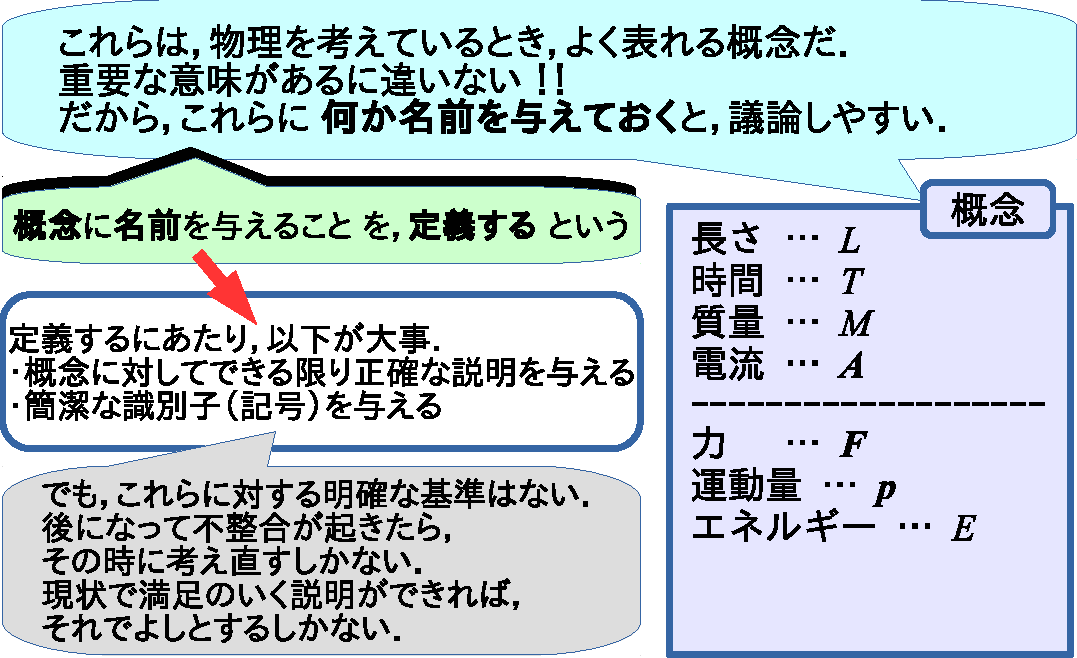
\includegraphics[keepaspectratio, width=6.5cm,height=4cm,clip]{teigi.pdf}
                            \caption{定義しよう!!}
                            \label{fig:teigi}
                        \end{center}
                    \end{figure}

                もちろん,定義した物理量が妥当でなかったと分かった場合,その定義を
                見直さなければならない.妥当でないというのは,実験事実と矛盾するこ
                とや,あるいは,全く的外れな定義等である.このようなことは,理論を
                作っていく上で必ず生じることであり,やむを得ない.

                このノートで定義される物理量は昔からその正しさが確認されているもの
                であり,従って,このノートで定義される物理量は今後も変化することが
                ないだろう
                    \footnote{
                        万が一,理論や実験技術の発展によって変更されることが余儀な
                        くされても,それは特殊な状況であるようなときに限って,定義
                        しなおされる.例えば,運動量  $\textit{\textbf{p}} = m\bv$ を
                        もつ物体はその速度が光速(光の速さ)に近いとき,相対性理論に
                        よってこの定義は見直される.詳細は,相対性理論の章を参照.
                    }.

                このノートでは「$\cdots$ と定義する」とは書かずに,「$\cdots$ という」
                と書くこともあるだろうが,これも定義のうちに入る と考えてもらいたい.

                また,物理量の定義を把握するためには演習が必要である.新しい概念が
                定義されたときは,演習書を用いてより感覚的に捉えられるようにしてお
                くとよい.先ほども書い通り,このノートで演習するようなことはない.

            \begin{memo}{「定義」の定義}
                「定義」という言葉の意味を,説明した.しかし,「定義」という語彙の
                定義をしたわけではない.単に,「定義」という難し言い回しを,噛み砕
                いて,言い直したに過ぎない.ならば,「定義」という語彙の定義は,
                どうなされるのだろうか,という疑問が浮かび上がってきたかも知れない
                    \footnote{
                        あるいは,ここの記述を読んで,疑問が提示され,不思議に思ったかもしれない.
                    }.


                しかし,実は,この疑問は意味のない疑問である.
                ゲーデールの定理などで有名な,自己言及が含まれていて,矛盾がおこるからである.
                「定義」という言葉を知らないと
                    \footnote{
                    ここでいう,「知る」という言葉は,
                    「定義」という語彙を,自分の頭で了解し,言葉で表せなくとも,感覚的に定義されている
                    ということを,念頭において使用した.
                    },
                「『定義』の定義とは何か」という疑問も起こりえない.
                一方で,「定義」という言葉の意味を知っているならば,そもそもこの疑問は起こりえない.
                    \footnote{
                        「『定義』の定義とは何か」とは何かという疑問をするためには,「定義」という言葉を
                        予め知っていないとならない.例えば,上の『定義』を一般的な語彙に拡張し,「Xの定義とは」
                        と置き換えてみるとわかりやすい.「Xの定義とは何か」と問うということは,すでに「定義」という
                        語彙を使用して疑問を投げかけているのであり,「定義」という語彙を了解した上での疑問と
                        いうことになる.そうなれば,X$=$「定義」とした時の,「『定義』の定義とは何か」という疑問を
                        投げるためには,やはり,予め「定義」という語彙を知っていないとなければならない.
                    }

                しかし,わからない.何をもって「定義」であると言えるのか.定義であるための基準とは
                何なのか.判断基準は定義と同じ意味であり,確かに,「『定義』の定義とは何か」という
                疑問と変わりなく思えるのだが,この疑問は自己矛盾を含んでいて,意味がないものである.

                私が今まで見てきた数学の解説書や参考書には,定義という言葉の意味を説明はされているものは
                あったが,定義であるための満たすべき基準が書かれたものは,見たことがない.

                どういうことだろうか.私の現在の解釈は,「定義」という語彙は名詞としてではなく,
                「定義する」という動詞として存在している,というものである.「定義する」という動詞は,
                ある語彙を,曖昧さなく
                    \footnote{
                        「曖昧」という語彙の意味も曖昧だ.ここでは,後の議論に論理的に相反する結果を
                        起こさない程度,と認識してもらいたい.
                    },
                より明確に意味づけを行う行為である,と考えるのだ.
            \end{memo}

%   %==========================================================================
%   %  Section
%   %==========================================================================
    \section{物理学の基本概念}
%       %======================================================================
%       %  SubSection
%       %======================================================================
        \subsection{物理量}
            物理的に意味のある量
                \footnote{
                    物理的に意味のある量とは,
                    「そのような量を導入することで現象がうまく説明できる」
                    という量である.
                }
            を \textbf{物理量} という.例えば,速度や加速度,重さ,長さ,時間などだ.
            運動量や力積,エネルギーや仕事量なども物理量である.実験により観測できる量
            は,すべて物理量であると思ってよい.

%       %======================================================================
%       %  SubSection
%       %======================================================================
        \subsection{物体}
            いままで,「もの」という表現を使っていたが,これからはもっとかっこよ
            く,\textbf{物体} ということにしよう.こっちのほうが,なんだか畏まっ
            てして,学問をしている感じになる.何でも難しく言えばいいということで
            はないのだけども,暗黙の了解をその言葉に含めるにはちょうどよいので
            ある.

            ここで,「物体」と表現したときに,暗黙の了解とされている性質を説明し
            よう.

            「もの」には,さまざまな性質がある.形,色,硬さ,におい等.また,そ
            の「もの」が食べ物であったなら,食感や味,風味もある.動物であれば,
            暖かさとか,おとなしいとか落ち着きがないとかなどの性格も,考えられる
            はずだ.一口に「もの」といってしまえば,こういう性質を全て考えなけれ
            ばならなくなる.けれど,これではあまりにも広い範囲の対象を相手にしな
            ければならず,一度に相手にするにはとても難しい
                \footnote{
                    難しい:不可能なことでない.「難しい」と表現されたときには,
                    原理的には可能なのであるが,実際に行うととても時間がかかる,
                    ということを意味している.例えば,「難しい問題」という表現が
                    ある.難しい問題とは,とくのに非常に時間のかかる(どれくらい
                    時間がかかるかは問題による)問題のことである.決して解けない
                    問題ではないのだ.まあ,そもそも「解けない問題」は問題ではな
                    い.だって,答えがないということがわかっているのだから(哲学
                    てきに難しい問題といわれたら,「“答え”のない問題」なのかも
                    知れないが).
                }.
            そこで,考える「もの」に制限を与えて,対象の範囲を狭くするのである.
            その制限とは,色とか,におい,味,食感,性格等は無視するということで
            ある.主に考えるのは,重さ,形,硬さである.どれに着目するかは,その
            つど異なるが,とにかく全ての性質を同時に扱うことは,難しいのでやらな
            い.

            特に,\textbf{物体} と言われたときには,「もの」の大きさと形しか考え
            ず,においとかの他の性質は全く考慮しないことを,暗に主張する.物理
            学でいう「物体」とは,日常生活で使用する言葉の“物体”とは異なる
                \footnote{
                    日常生活で使用する“物体”と同じ意味で,今まで「もの」と表現
                    していた.
                }.


%       %======================================================================
%       %  SubSection
%       %======================================================================
        \subsection{系}
            考える対象全体のことを \textbf{系} という.例えば,$N$ 個の物体の運動
            について考えるときに,「系全体」といわれたならば,それは,「$N$ 個の
            物体に関わるもの全て」ということ と同じ意味である.

            例えば,積み木が積まれている台車が運動しているとしよう.この台車がど
            のような動きをするのかを考えるとき,この積み木と台車の両方について考
            える必要がある.このときの系全体とは,「台車と積み木」である.太陽に
            対する地球の自転を考えるときの系全体とは太陽と地球のことである.より
            正確には周囲の他の惑星も系とすべきだ.要するに,今何を対象に考えてい
            るかとか,何に注目しているだとかの,そのような対象(もの)を総じて系と
            いうのだ.

%       %======================================================================
%       %  SubSection
%       %======================================================================
        \subsection{文字・数式・式変形}
            \begin{mycomment}
            物理学において,数式とは推論の道具に過ぎない.しかし,それは途方も
            なく有用な道具である.数式の持つ意味について,考える.
            \end{mycomment}

        \begin{mysmallsec}{文字}
            数式は文字で表現される.そして,文字は互いに関係付けられている.具
            体例で考える.ここに一冊の本があるとする.本には色々な性質が備わ
            っている.重さや色,紙の質,書かれている文字,匂い等,色々とある.
            物理学では,これら本のもつ諸性質のうち,特に関心があるのが,重さで
            ある.そこで,ここでは本の重さのみについて考えることにし,その他
            の性質(匂いやその記述されている内容)は全く無視してしまおう.それ
            で,本の重さについての記述をしたいのだが,どうすればよいだろう.
            なんて問うまでもなく,「重さを $W$ とおく」と表現すれば良い.「重さ
            を $W$ とおく」と表現したことにより,現実にある本の重さが,文字 $W$ で
            表現され,重さを数学的に扱うことが可能になった.視点を数式目線に変更
            して考えて見れば,文字 $W$ に重さという意味が与えられたとも考えるこ
            ともできよう.
        \end{mysmallsec}


        \begin{mysmallsec}{数と数字}
            ものの個数
                \footnote{
                    例えば,りんごの個数だとか,鉛筆の本数だとか,本の冊数だとか,
                    家の件数だとか,
                }
            や物の値段などで使われる,概念を抽象化したものを \textbf{数} という
                \footnote{
                    「スウ」と読む.「カズ」と読んでも間違いではないが,
                    数学をしている時には「スウ」と言う方が一般的.
                }.

            "数" を文字で表したものを \textbf{数字} という.同じ数に対して,
            いろいろな字が割り当てられていて,例えば,以下はすべて同じ数を示す文字である:
                \begin{equation*}
                    4 \,, \qquad \mbox{四} \,, \qquad \IV
                \end{equation*}
            数を表す文字は複数種類あり,どれを使っても良い.
            一般的に,\textbf{アラビア数字} と呼ばれる以下の数字が便利であり,多く使用される:
                \begin{equation*}
                    0 \, , \quad  1 \, , \quad  2 \, , \quad  3 \, , \quad
                    4 \, , \quad  5 \, , \quad  6 \, , \quad  \ldots
                \end{equation*}
            数式内の数字はアラビア数字を使う.文章内の数字はアラビア数字も使用するが,
            \textbf{漢数字} も使用する.漢数字とは,以下のような数字である:
                \begin{equation*}
                    \mbox{一}\, , \quad \mbox{二} \, , \quad \mbox{三}   \, , \quad \mbox{四} \, , \quad
                    \mbox{五}\, , \quad \mbox{六} \, , \quad \ldots
                \end{equation*}
            他にも,\textbf{ギリシア数字} ($\I$,$\II$,$\III$,$\IV$,$V$,$\VI$,$\ldots$) も数字だし,
            「正」の字を使って数えるときの途中段階の文字(記号?)も数字である.まあ,色々とあるが,
            物理学を勉強していく上では,上記のような常識的な範囲の数字の扱い方ができていれば十分である.
        \end{mysmallsec}

        \begin{mysmallsec}{変数}
            具体的な数($1,\,2,\,3,\,\ldots$)ではなく,"全ての数に対しての記述"をしたい場合がある
                \footnote{
                    数全般の性質を表したい場合は,具体的な数字を使って表現するわけににはいかない.
                    具体的な数字を使ってしまうと,その数にしか成り立たない記述になってしまう.
                }.
            そういった場合,\textbf{変数} という考え方を使う.
            全ての数に当てはまるということは,どんな数にも変わり得るということ.
            変数を表す記号は,様々である.
            中学や高校数学では,$x$ や $y$ や $z$ が使われる.また,$\theta$ や $\phi$ などの
            ギリシャ文字を使うことも多い.

            もっと高度な数学になると,
            変数が無限に多く欲しい場合があり.その場合は,アルファベットでは対応できない.だから,
            以下のように,アルファベットの右下や右上にアラビア数字を添えて,
                \begin{equation*}
                    {x}_{1} , \quad {x}_{2} , \quad {x}_{3} , \quad \ldots
                \end{equation*}
            と言った感じで,無限に変数を増産できる
                \footnote{
                    あるいは,
                    \begin{equation*}
                        {x}^{1} , \quad {x}^{2} , \quad {x}^{3} , \quad \ldots
                    \end{equation*}
                    でもよい.添字は右上でも右下でもどちらでも構わない.今のところは,
                    添字の位置には特に意味を与えていないが,後々(相対性理論を勉強する段階)では,
                    この添字の位置に意味を与えるので,注意が必要だ.
                }.
            添字は無限に増やせるからだ.だが,これでも,
            変数を無限に列挙することなどはできない.そこで,「$i$ は任意の自然数であるとする」という
            文言を添えて,
                \begin{equation*}
                    {x}_{i}
                \end{equation*}
            の一文字で済ますことが可能である
                \footnote{
                    $i$ には 1でも2でも99でも何でもよく,とにかく全ての自然数が順に与えられて,
                    整列させられているイメージを持って欲しい.そのイメージを具体的に書くと,${x}_{i}$ と
                    書かれた場合,
                    \begin{equation*}
                        {x}_{i}
                        \leftrightarrow
                        \left( 1,\,2,\,3,\,4,\,5,\,6,\,\ldots,\,i,\,\ldots,\,\infty \right)
                    \end{equation*}
                    ということである.$\leftrightarrow$ はその左側と右側で同じ意味を持つことを示す
                    ものである.

                    また,ここで,\textbf{無限} について定義せずに使用しているが,普段の
                    生活の意味の無限として捉えていて問題ない.無限を真面目に考え始めると,
                    深みにハマってしまい,議論が終わらなっくなってしまう.無限についての理解は
                    この程度で十分であろう:
                        \begin{equation*}
                            \mbox{無限大 とは,全ての数よりも大きい ということである.}
                        \end{equation*}
                        \begin{equation*}
                            \mbox{無限小 とは,全ての数よりも小さい ということである.}
                        \end{equation*}
                    "ということ" と表現したのには意味がある."という数" と書いていしまうと,
                    自己言及して矛盾になってしまう,「"全ての数" よりも大きい"数"」なんて
                    文は矛盾.だって,"全ての数"って言っているんだから,これよりも大きい数って,
                    全ての数以外の数だということになって,つまり,「"全ての数"以外の数」があることになる.
                    「"全ての数"以外の数」なんてものは矛盾.要するに,無限を数として扱ってはならない
                    ということである.
                }.

            変数の例を上げると,$f(x)=ax+b$ や $g(\theta)=\sin\theta$ と書かれた時の,
            $x$ と $\theta$ がそれに当たる.この場合の $x$ と $\theta$ は関数の定義域の全ての
            実数値を取りうることを意味付けられている.
        \end{mysmallsec}

        \begin{mysmallsec}{定数}
            ある特定の数(固定された値)であるが,それが特別な数ではない場合,これを \textbf{定数} という.
            読み方は,「ジョウスウ」または「テイスウ」である
                \footnote{
                    普通は「テイスウ」と読む.年齢を重ねた人が「ジョウスウ」と読む,という勝手なイメージがある.
                }.

            低すを表す記号として,アルファベットの最初の文字 $a$,$b$,$c$,$d$ などが使われる.大文字の $A$,$B$,
            $C$ が使われることも多い.変数に比べると,様々な文字が定数を表す記号として使われる傾向にある.
            ただ,教科書にはその都度,それが定数であるか変数であるかを説明しているので,どっちかわからずに混乱
            することはないだろう.

            先にも上げた例だと,$f(x)=ax+b$ とした場合の,$a$ や $b$ が定数である.
        \end{mysmallsec}

        \begin{mysmallsec}{整数(自然数,負の数),有理数}
            このノートでは,$0$ を含めた以下を \textbf{自然数} とよぶ:
                \begin{equation*}
                    0,\,1,\,2,\,3,\,4,\,5,\,6,\,7,\ldots
                \end{equation*}

            負の数とは,ある定数 $A$ に対して $A+x=0$ となるような $x$ のことをいい,$x:=-A$ と
            書く慣習がある.例えば,$A=1$ の時は,$x=-A=-1$ だし,$A=100$ だったら,$x=-100$ である.

            自然数と負の数を大きさ順に具体的に並べてみると,以下のようになる(右にあるほど大きい):
                \begin{equation*}
                    -4,\,-3,\,-2,\,-1,\,0,\,1,\,2,\,3,\,4\ldots
                \end{equation*}
            記号 $-$ のことを,\textbf{マイナス} とう.「負の数」という新たらしい数が作られたことで,
            今まであった0以外の自然数のことを \textbf{正の数} とよぶこともあり,記号は $+$ を使う.
            記号 $+$ は\textbf{プラス} という.「マイナス」と「プラス」は英語のplusとminusであり,
            "正"と"負"はこの英語に対して割り当てられた日本語語彙である.
            自然数と負の数を総称して,\textbf{整数} という.

            整数を2つ用意して(用意した2つが同じ整数でもいい)以下のように表した時,
            これを \textbf{有理数} という:
                \begin{equation*}
                    \frac{1}{2} \;,\;\; \frac{-9}{123} \;,\;\; \quad \frac{4}{-5} \;,\;\; \quad \frac{-9}{-177}
                \end{equation*}
            上記のように,真ん中に短い線を引いて2つの数を上下に記述した有理数の表現手法を \textbf{分数} という
                \footnote{
                    分数を一行で記述したい場合もある.こういう時は,1/2 とか -9/123 などと書く.
                    記号"/"を数の間に入れて分数を表現するのである.
                }.
            0 は下に書くことはできない
                \footnote{
                    0を下に書くと,四則演算で論理的に不整合な計算ができてしまい,体系に矛盾が生じる.
                    例えば,$\frac{1}{0}$ という数を書いてみる.
                    どんな数でも0をかければ,0になるので(これは0元の公理で,有無を言わずに認めることである),
                    $\frac{1}{0} \times 0 = 0$ となるのだが,この式の左辺は $\frac{1}{0} \times 0 = 1$ とも計算できる.
                    すると,$1=0$ となって論理的に不整合(矛盾)になる.矛盾が生じた理由は,
                    そもそも $\frac{1}{0}$ という数が存在すると仮定したからである.要するに矛盾を起こさないためには,
                    $\frac{1}{0}$ というような分母に0を置くような有理数(分数)を考えてはいけないということだ.
                }.
            また,上の数のことを \textbf{分子} といい,
            下の数のことを \textbf{分母} という.分子と分母の両方が負の数の時は,
            その両方のマイナスを取り去っても同じ分数としてあつかう:
                \begin{equation*}
                    \frac{-9}{-177} = \frac{9}{177}.
                \end{equation*}
            分母と分子のどちらか一方のみが負の数の場合は,負の分数として扱い,マイナス記号を
            分数の左真ん中へ移動させて書く:
                \begin{equation*}
                    \frac{-9}{123} = \frac{9}{-123} = -\frac{9}{123}.
                \end{equation*}

            分数の具体的なイメージは,割合だろう.全体の数を分母とし,分子には今注目している部分の数を書く.
            こうしてあらわされた分数は,注目している箇所は全体のどれくらいかを示す量となる
                \footnote{
                    あくまでも,分数を現実と対比させたい場合の例である.
                    数学では,このような具体的なイメージから発展させ,より抽象化される.
                    この例にとらわれると,マイナスの数が分母に書かれたときに,全体の数がマイナスになるが
                    どういうことだろうかと,無駄な考えに陥るかもしれない.数は現実の世界から必要に迫られて
                    人間が生み出したものであるが,数学ではそれを抽象化して数の性質を探求する学問である.
                    現実との具体的な対比に悩むのはナンセンスだ(物理学では大事なことだが).
                }.
        \end{mysmallsec}

        \begin{mysmallsec}{等号,不等号}
            2つの数を比較して,どちらが大きいか(あるいは小さいか)を文字で書きたいことがある.
            その場合,2つの数 $a,\,b$ を比較して,$a$ が $b$ よりも大きい場合は $a>b$ または $b<a$と書く.
            $b$ の方が $a$ よりも大きい場合は $a<b$ または $b>a$ とかく.$a$ と $b$ が
            等しい場合は $a=b$ とかく.記号にも名前があり,$=$ を \textbf{等号} といい,
            $<,\,>$ の2つを \textbf{不等号} という.不等号が2種類あると思われるかもしれないが,
            向きをどうするかの($a$ と $b$ の並べ方)違いであり,実際上,1種類記号である.
        \end{mysmallsec}

        \begin{mysmallsec}{演算,演算器号}
            演算には,「加算」と「乗算」がある.加算は記号 $+$ で表され,乗算は記号 $*$ で表される.
            加算と乗算はどういった計算かを一般的に示すことはできないので,以下に具体例を書くに留める.
            \begin{equation*}
                \mbox{加算: } 1+1=2 ,\quad 12=6+3+2+1
            \end{equation*}
            \begin{equation*}
                \mbox{乗算: } 1*1=1 ,\quad 36=6*3*2*1
            \end{equation*}

            加算と乗算以外にも,減算と除算があると思われるかもしれないが,減算と除算は加算と乗算の一部
            として含めることができる.減算の場合には,加算に対して負の数を導入することで,実現できる.
            つまり,
            \begin{equation*}
                \mbox{減算: } 1-1=1+(-1) , \quad 4=6+(-3)+2+(-1)
            \end{equation*}
            のように,減算ではなく負の数との加算だと解釈すれば,減算は加算のとみなせる.
            除算の場合には少し強引に聞こえるかもしれないが,分子を1とする分数と整数の除算,つまり,
            \begin{equation*}
                \mbox{除算: } 1 \divisionsymbol 2=\frac{1}{2}=1*\frac{1}{2} ,\quad 5 \divisionsymbol 6=\frac{5}{6}=5*\frac{1}{5}
            \end{equation*}
            と考えることで,除算を乗算の一部とみなせる.

        \end{mysmallsec}

        \begin{mysmallsec}{数式}
            世の中には非常に多くの本がある.本だけではない.鉛筆,ボー
            ルペン,コンパス,定規,机の上にあるものだけ上げても,非常に多くの
            ものが存在している.話を簡単にするために,机の上には,鉛筆と消しゴ
            ムと本がそれぞれ一つずつ存在し,これ以外のものは置いていないとしよ
            う.やはりこの3つのモノにも重さがあり,それを $W_{\mbox{鉛筆}}$,$W_{\mbox{消しゴム}}$,
            $W_{\mbox{本}}$ と表現することにしよう.これら3つの重さについて関心がある
            のは,それらの「関係」だろう.「関係」といったのは,どれが最
            も重いかとか,軽いかといったことである.この「関係」を数学的に扱
            うには,数式を使うと非常に簡単に表現できる.例えば,鉛筆の重さと消
            しゴムの重さが全く同じ時には,
                \begin{equation*}
                    W_{\mbox{鉛筆}} = W_{\mbox{消しゴム}}
                \end{equation*}
            と表現できることは,周知のことであると思う
                \footnote{
                    哲学的な疑問はここでは考えないことにしよう.数式は文字の羅
                    列である.ここで言うと,
                        \begin{center}
                            $W$,$=$,鉛,筆,消,し,ゴ,ム
                        \end{center}
                    という記号の羅列と捉えられる.文字の羅列になぜ意味を感じるの
                    か.うーん,難しい.とりあえず,この疑問は保留にしておこう.
                }.
            数式とは,文字と文字の「関係」を表現できるものである.
        \end{mysmallsec}

        \begin{mysmallsec}{式変形}
                        文字と数式には意味があり,特に物理学において文字と数式は,現実
            世界と強く結びついている.現実に起きている現象を数式で表すことが,物
            理学のひとつの方法なのだから.では,「式変形」に意味はあるのだろうか.
            結論から言えば,「式変形」それ自体にはなんの意味もない.単に,数学
            的に定義された文字の操作を行っているに過ぎない.にもかかわらず,「式
            変形」は非常に重要なのである.実際,式変形を行うことにより,いろいろ
            と推論を行うことができるし,また,それによって物理学が発展しているの
            である.意味が無いのに重要であるとは,いったいどういう事なのか.答え
            は,式変形を行うことにより,論理的必然性を確かめることができることに
            ある.何らかの意味をもった数式に式変形を施すことで,別の意味の数式を導出す
            る.これにより,正しい推論を行うことができるのである.世の中には論理
            的に矛盾したことは起こりえないから
                \footnote{
                    そもそも,論理的に矛盾していることを想像することもできない.
                    「ここに本があり,かつ,その同じ場所に本がない」という状況
                    を思い描くことが可能だろうか.
                },
            論理立てて考えることで,間違った結論を出すことは,ぐっと少なくなるは
            ずである.式変形を行うということは,論理的推論を行うということであり,
            そうして得た結論は,論理的に必然性を持つものであり,実験して確かめる
            価値は十分にあると言える.ちなみに,ここで言う必然性とは,物理学的に
            考えて必然ということであり,論理的に厳密に必然であることをいうのでは
            ない.物理学における論理的推論とは,「物理学的に考えてもっともらしい仮定」
            をもとにするため,この点において多少の厳密性が犠牲にされている.
        \end{mysmallsec}


        \begin{memo}{$a+b=b+a$ ?}
            $4+3=7$という足し算を考えよう.当然,$3$と$4$を入れ替えて書いて,$3+4=7$と書いても同じ.
            また,等号の右と左を入れ替えて,$7=4+3$あるいは,$7=3+4$としても,等式は成り立つ.
            本当にそうだろうか.$3+4$は$4+3$に同じなのか.実際のところ,違うだろう.
            3つのイチゴと4つのリンゴは,4つのイチゴと3つのリンゴとはことなる.
            確かに,個数だけに着目すれば$3+4=4+3$になるが,イチゴとリンゴの個数としての数字であると
            考える場合には,この等式は成り立たない.
            また,$3+4=7$という式を言葉にすると「3足す4は7である」と表現するのが自然であり,
            他方,$7=3+4$は同じように言い表すと「7は3足す4である」となる.両者の意味は全く違う.
            「7は3足す4である」は間違ってはいないが,決めつけているような表現であり,抵抗を感じる
                \footnote{
                    $7=5+2$でも,$7=1+6$でも,$7=10-3$でもよいのである.
                }.
            $3+4$も$4+3$も$5+2$も$10-3$も数式として考えれば,計算結果はすべて等しく,7である
                \footnote{
                    $3+4$という計算結果と,$4+3$という計算結果が等しく,両者とも互いに置き換えることが
                    できるということ.
                }.
            式計算する場合に,数や式に意味を考えてしまうと,余計なことを考え出してしまう(「$4+3$と$3+4$は同じか」とか).
            式計算時には数を抽象化してとらえなければならない
                \footnote{
                    きっとここら辺に数学の素晴らしさがあるのだろう.
                    こういう抽象化が興味深い体系的の数学を構成する基礎になっていくのだと感じる.
                }.

            一方で,物理学では単位という概念がある
                \footnote{
                    長さ[m],時間[s],質量[kg],電流[A]など.
                }.
            物理学で扱う数字には意味が込められており,計算時に単位を意識する必要がある.
            単位が違う数字の足し算は認められていない
                \footnote{
                    長さ1[m] + 質量1[kg] という計算は全く意味不明だ.
                }.
            掛け算は認められている
                \footnote{
                    だからこそ,新しい概念を作ることができる.
                    エネルギーの単位[J]は,力1[N]と長さ1[m]の積として定義されている.
                    ($[\mbox{J}] := [\mbox{N} \cdot \mbox{m}].$)
                }.
            単位は数学にはない概念である
                \footnote{
                    ここにも,科学と数学の違いが表れている.
                }.
            物理学で数式を扱う場合,数学と全く同じように扱ってしまうと,
            単位の違う数字の足し算をしてしまうという誤りをしがちである.
        \end{memo}



%===================================================================================================
%  Chapter : 力学の基本概念
%  説明    : 力,重ね合わせの原理,力(作用)の種類,単位などの基礎概念について説明する.
%===================================================================================================
\chapter{力学の基本概念}
%   %-----------------------------------------------------------------------------------------------
%   %  Input
%   %    File Name : PhysNote_CM_MechIntro.tex
%   %    説明      : 物理学の基本的な考え方(定義,法則等)について説明する.
%   %-----------------------------------------------------------------------------------------------
%===================================================================================================
%  Chapter : 力学の基本概念
%  説明    : 力,重ね合わせの原理,力(作用)の種類,単位などの基礎概念について説明する.
%===================================================================================================
%   %==========================================================================
%   %  Section
%   %==========================================================================
    \section{力とその性質}
%       %======================================================================
%       %  SubSection
%       %======================================================================
        \subsection{力(ちから)}
            世の中には,\textbf{力} といわれる現象がある.この「力」は様々な意味
            合いで使用される.視力,脚力,握力などの身体能力に関する「力」.計算
            力,想像力などの思考に関する「力」.ほかにも,技術力,接客力,情報収
            集力,対応力など,人の性格や能力に関する「力」などいろいろ考えられる.

            物理学で対象とする \textbf{力} は,弾性力や反発力,物体を変形させる力,
            物体の運動方向を変化させる力などである.以下,「力」と表現される場合
            には,特に断りのない限り,このような力を想定する.

            力とは,捕らえ所がなく,非常に曖昧である.現に,ニュートン力学では,
            力とは何かを説明することはできない.では,どのように力というものを
            考えるのか.結論から言うと,力の存在を,なんの根拠もなしに認めること
            である.力という物理現象の発生原因が分からないのだけど,実際に,
            私たちは日常的に,力が存在しているということに関して,疑いを持つこと
            はない
                \footnote{
                    力の存在に疑問をもつこともあることだろう.しかし,ここ
                    では哲学について語っているのではない.力とは何か,も
                    っと言うと,力という現象を感じる私たちとは何なのか,こ
                    れはひどく難しい問題である.なので,こういう問題には目
                    を閉じておくことにしよう.今の私の興味は,世界がどのよ
                    うに構成されているかということであり,こんなところで,
                    足を止めてしまってはならない.知りたいことはもっと先に
                    ある.そのために,力という現象の存在を素直に認めること
                    にしよう.ただし,この問題を忘れてはならない.ノートの
                    端の方に,「力とは何か」という疑問をメモしておこう.
                }.

            しかしながら,力は重要な概念である.
            力学の最大の目標の一つは,物体の運動の軌道を求めることにある.
            それには,物体にかかっている力を,考えないとならない.
            物体の運動の原因は力であり,力は
            物体の運動を解析する上で,非常に重要なものである.

            これだけ重要な概念である“力”なのだけど,「力とは何か」と問われると,
            回答するにはとてもむづかしい
                \footnote{
                    素粒子物理学の教科書などでは,(ゲージ粒子を介した)「相互作用」と
                    説明されるが,詳細は,素粒子物理を考えるときに説明しよう.
                }.
            とりあえずの力の説明として,物体を変形させる,あるいは,物体の位置を
            変化させる原因としておこう.言い換えると,物体が変形すれば,その物体に
            力が加えられたということになるし,物体の位置が変化したならば,この場合にも
            物体に力が加えられたということになる.

            物体の変形や変位を説明する概念として,力の存在が要請されるとしてもよい.

%       %======================================================================
%       %  SubSection
%       %======================================================================
        \subsection{力の重ね合わせの原理}
            複数の力が物体に働いているとき,その力を合計することを,
            力の \textbf{合成} という.合成された力のことを \textbf{合力} という.
            力の合成は,ベクトル和 で表現できる.すなわち,物体に $N$ 個の力が加わっているとき,
            その合力は,
                \begin{align}
                    \bF_{\mbox{合力}}
                    = \bF_{1}+\bF_{2}+ \cdots + \bF_{N}
                \end{align}
            である.和の記号を用いると
                \begin{align}\label{gouryouku_gouryoku}
                    \bF_{\mbox{合力}} = \sum^{N}_{i=1} \bF_{i}
                \end{align}
            のようにかける.

            また,逆に,1つの力を,複数の力の合力である
                \footnote{
                    式(\ref{gouryouku_gouryoku})は等式であり,
                    左右が等しいのだから明らかではあるが,
                    少しだけ気付きにくいかと思われたので書いておいた.
                    すなわち,1つの力を複数の力に \textbf{分解} することもできる.
                    }.
            力の分解は,よく行われる.例えば,$x-y$ 平面上における力を表現するのに,
            力を $x$ 方向と $y$ 方向に分けて考えることが多い.
                \begin{figure}[hbt]
                    \begin{center}
                        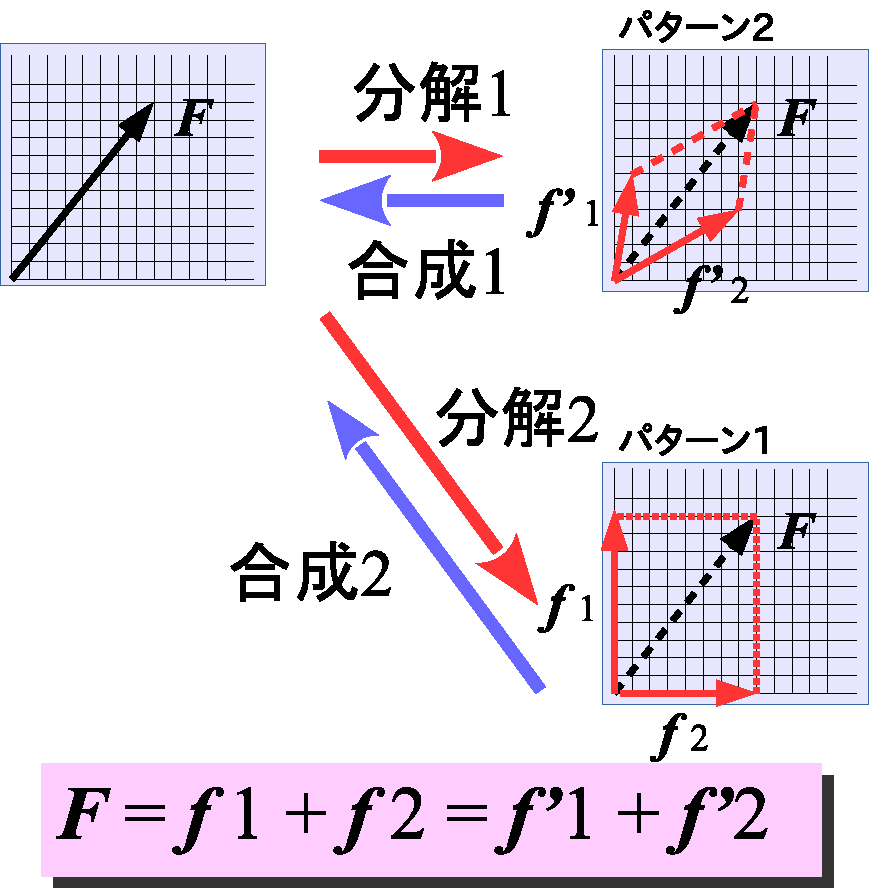
\includegraphics[keepaspectratio, width=6cm,height=6cm,clip]{f_bunkai.pdf}
                        \caption{力の合成,力の分解}
                        \label{fig:f_bunkai}
                    \end{center}
                \end{figure}

            力学では,力が重ね合わせの原理を満たす理由は問わない.
            この原理は,実験的に確かめられる法則として扱われている
                \footnote{
                    もしかしたら,将来,このことを説明できる日が来るかもしれないが,
                    今はこれを説明できるだけの知識がない.ただ,電磁気力に関していえば,
                    電磁場の線形性に帰着できる(問題を先送りしただけ,かもしれないが).
                }.

            別称として,\textbf{平行四辺形の法則},\textbf{力学の第0法則} とかと表現されることもある.
            重ね合わせの原理が成り立つことを,数学的に表現すると,「力には \textbf{線形性} がある」ともいえる.
            もっと物理学の学習を続けていけば,力の重ね合わせの原理を
            説明できるようになるのかもしれない.しかし,ここではその理由はわからないので.
            とりあえず,重ね合わせの原理を認め,学習を先に進めるべきだ.

              \begin{memo}{和の記号: $\sum$}
                例えば任意の4つの実数 $a_{0},\,a_{1},\,a_{2},\,a_{3}$ が与えられたとする.
                この時,$a_{0}$ から $a_{3}$ までの和 $S$ を書き表すとき,
                  \[
                    S = a_{0} + a_{1} + a_{2} + a_{3}
                  \]
                のように書き表せる.しかし,項数が9999個になった場合($a_{1},\,a_{2},\,\cdots\,a_{9999}$ ),
                書き表すことはできない
                  \footnote{
                    原理的には可能であるが,実際に書くのに時間がかかるため現実的ではない.
                  }.
                そこで,$a_{0}$ から $a_{9999}$ までの数の合計を計算することを示す記号を導入したくなる.
                和の記号として,$\sum$ を新たに導入し,以下のように記述することにしよう.
                  \[
                    \sum^{9999}_{i=0} a_{i} := a_{0} + a_{1} + a_{2} + \cdots + a_{9999}.
                  \]
                $\sum$ は「シグマ(Sigma)」と発音する.
                今の例だと上限が9999の場合に限ってしまうが,上限を任意の数 $N$ として場合には,
                次にように書く
                  \footnote{
                    前の例だと具体的な数字だった9999を $N$ という文字に変更する.
                  }.
                  \[
                    \sum^{N}_{i=0} a_{i} := a_{0} + a_{1} + a_{2} + \cdots + a_{N}.
                  \]
                さらに,この例だと最初の数字は0であるが,もちろん任意でよい.
                最初の数を $m$ と文字で置き換えて($m<N$であるはず),
                  \footnote{
                    例えば,$a_{0},\,a_{1}$ がべっと定まっていて,この2つの数にさらに
                    $a_{2}$ から $a_{N}$ までの数の合計を足したいこともありうる.
                  }
                  \[
                    \sum^{N}_{i=m} a_{i} := a_{m} + a_{m+1} + a_{m+2} + \cdots + a_{N}.
                  \]
                  これで,項数が多くなっても和を書き表せるようになった.

                  ちなみに,$a_{i}$ の添え字 $i$ は和の具体的な計算(和の記号の展開)の時に,
                  失われてしまう数で\textbf{ダミー}の数字と言われることがある.別に $i$ ではなく,
                  $j$ を使ってもよい.
                  その場合は以下のようになるが,$i$ の場合と意味は同じである.
                  \[
                    \sum^{N}_{j=m} a_{j} := a_{m} + a_{m+1} + a_{m+2} + \cdots + a_{N}.
                  \]

                  項数を無限大 $\infty$ にした場合でも,
                  \[
                    \sum^{\infty}_{j=m} a_{j} := a_{m} + a_{m+1} + a_{m+2} + \cdots
                  \]
                  と形式的に表現することもできる
                    \footnote{
                      「形式的に」といったのは,$\infty$ が数ではないために,正式な和の手続きに
                      なっていないからである.しかし,この表現により,無限にある項数を順に足し合わせる
                      という行為をイメージさせることが可能である.
                    }.
              \end{memo}


%       %======================================================================
%       %  SubSection
%       %======================================================================
        \subsection{作用}
            力のことを,場合によっては,\textbf{作用} ということもある.
            例えば,「2つの物体間に働く相互作用」と書かれていたら,
            これは,2つの物体に働く力という意味である
                \footnote{
                    量子力学や素粒子理論,あるいは,一般相対性理論の教科書でよく使われる表現だ.
                    ニュートン力学でも,「作用$\cdot$反作用の法則」のように使用されれる.
                }.

            宇宙論や素粒子理論の教科書などでは,その冒頭に「力には4つの種類ある」
            と紹介さることが多く,\Table\ref{table:f4force} が掲げられる
                \footnote{
                    当然ながら,この力の分類は,物理学の発展により得られたものであり,
                    最初から知られていた事実ではない.
                }
            この4つの力は,それそれで従っている物理法則や性質が異なる.
            つまり,少なくとも4つの物理法則があるということであり,
            だけどこれは,物理法則はただひとつであるという物理学の精神に反する.
            物理学の理論構築の目標の一つは,この4つの力を自然に説明することである.
            要するに,4つの力を説明できるような,もっと大きな理論的枠組みを構成し,
            その枠組みの中で4つの力が自然に導かれるような理論を作りたいのだ
                \footnote{
                    今では,電磁気力と弱い相互作用と強い相互作用の3つの力を説明できる
                    統一理論が知られいて,これを \textbf{標準模型} という.しかし,
                    標準模型には人為的な定数が多く含まれており,また,万有引力も
                    説明できないので,私達が知りたい力の統一理論ではない.

                    当然ながら,力を統一的に説明できるという保証はどこにもない.
                    統一理論の確立は可能であると信じて,理論を作り上げる努力をするしかない.
                    超弦理論は,現状での最も有力な理論の1つであるが,超弦理論を実験的に検証されていない.
                    他の候補にもループ量子重力という理論も提案されているが,こちらも実験検証ができていない.
                    一般に周知される理論の確立にはまだ時間がかかるようだ.
                    もしかしたら,その過程で,力を統一的に説明できない,という結論に至る可能性もある.

                }.

                 \begin{table}[htb]
                  \centering
                  \caption{4種類の力}
                  \begin{tabular}{|l|c|}           \hline
                    名称         & 別称         \\ \hline  \hline
                    万有引力     & 重力         \\ \hline
                    電磁気力     & ローレンツ力 \\ \hline
                    弱い相互作用 & $\beta$崩壊  \\ \hline
                    強い相互作用 & 核力         \\ \hline
                  \end{tabular}
                  \label{table:f4force}
                \end{table}

            \begin{mysmallsec}{万有引力(重力)}
            万有引力はどんな物質も持っている性質で,その強さは,4つの内で最弱.
            重力とはが物を引っ張る力のことで,それは万有引力の一部であるが,
            重力という表現のほうが実感があり馴染み易いせいか,万有引力と同義的に
            使われることが多い.一般的に,万有引力と重力は同義であると考えてよい
                \footnote{
                    ただし,両者を区別して考えたい場合もあるので,文脈により判断したい.
                }.

            重力を説明する理論は一般相対性理論である.重力があまり強くない場合は,
            ニュートンの力学で十分精度よく説明される.
            \end{mysmallsec}

            \begin{mysmallsec}{電磁気力(ローレンツ力)}
            電磁気力は,ローレンツ力と言われることもある.ローレンツは電磁気現象の
            解明に貢献した物理学者の名前である.電磁場中を運動する電荷が受ける力の
            ことである
                \footnote{
                    詳しくは電磁気学の部分で学習する.
                }.

                        電磁気力は電磁気学,あるいは,電弱統一理論によって説明される.
                        電弱統一理論は電磁気力と次に説明する弱い相互作用の両方を説明できる理論である.
                        ただ,電磁気力のみを考える際には,マクスウェルの古典的な電磁気学
                        で十分な場合が大半.
            \end{mysmallsec}

            \begin{mysmallsec}{弱い相互作用}
            弱い相互作用とは,原子が$\beta$崩壊するときに使われる力である.原子核や
            素粒子を扱う場合に,重要な力だけれど,力学では対象範囲外の概念である.
            量子力学や特殊相対性理論(場の理論)によって説明される力である.
                        電弱統一理論によって説明される.
            \end{mysmallsec}

            \begin{mysmallsec}{強い相互作用(核力)}
            強い相互作用とは,原子核を構成する陽子と中性子を結びつける力である.
            陽子と陽子,中性子と中性子も強い相互作用によって引き合っている.
            電磁気力を考えると陽子同士は反発しあって安定しないのだが,この
            強い相互作用によって引き合うために,原子核が安定して存在できる
            だから,当然,強い相互作用は電磁気力よりも強い力である.しかし,
            単純にそう考えると,電磁気力は強い相互作用に隠されてしまう(
            表だって電磁気力を感じなくなってしまう)はずだが,実際はそうではない.
            その理由は,有効範囲の違いで説明される.原子核よりも狭い領域では
            強い相互作用が優勢であるが,原子核以上の範囲では強い相互作用は
            電磁気力よりも弱くなるのだ.
                        各力は,量子色力学によって説明される.
            \end{mysmallsec}

%       %======================================================================
%       %  SubSection
%       %======================================================================
        \subsection{外力}
            系の外から生じる力が系に影響を及ぼすこともあろう.対象とするもの以外
            から受ける力のことを \textbf{外力} という.例えば,重力に
            逆らって物体を持ち上げるときに,人間による力が必要である.物体が勝手
            に重力に逆らって宙に浮いたりすることはありえないからである.このよう
            に,人間による力を想定して,外力という言葉を使うこともある.

%   %==========================================================================
%   %  Section
%   %==========================================================================
    \section{基本単位 ([s]/[m]/[kg]/[A])}
%       %======================================================================
%       %  SubSection
%       %======================================================================
        \subsection{単位と測定}
            物理学は経験・実験結果がその基礎であることは前に書いた通りである.
            実験とは,実験すべき対象に何か刺激を与えて,その反応をみることである.
            このとき,対象の持っている何らかの量を測る必要が出てくる.ここで,「
            「測定とは何か」ということを考え直さないといけない.
            答えは簡単だ.
            \textbf{測定とは,基準値に対して何倍であるかを調べる行為である}と言える.
            言い方を変えれば,測定基準と測定対象の大きさを比較することである.
            測定対象は色々とあるが,例えば,音の大きさだったり,気圧,
            紐の長さ,ものの色,糖度,$\cdots$ etc,と色々ある.
            この比較対象となる基準値は,\textbf{単位} と呼ばれる.
            「基準値」という語彙は意味が広く,合格基準点とかのボーダーライン的な
            意味でつかわれることも多い.単位という特別な名称を与えたのは,基準値
            の意味を狭めるためである.単位とは,測定対象の大きさや量を数字で示す
            ための,最も基本的な大きさを規定するものである.

        \subsection{4つの基本単位}
            物理学では,以下の4つを,測定可能な最も基本的な量としている(\Table\ref{table:f4unit})
            \footnote{
                逆に言うと,この4つの単位は,他から導くことのできない単位である.
                いわば,単位系におけるもっとも素朴な要素となる.単位の素粒子的な
                役目を担っている.他の単位は,これらの単位から組み立てることが
                できる,というか,そのように定義される.
            }.
                \begin{table}[htb]
                  \centering
                  \caption{基本単位(物理学の基本4単位)}
                  \begin{tabular}{|l|c|c|l|}                  \hline
                    名称 & 記号   & 英字表記  & 読み       \\ \hline  \hline
                    時間 & [s]    & second    & セカンド   \\ \hline
                    長さ & [m]    & meter     & メートル   \\ \hline
                    質量 & [kg]   & kilo-gram & キログラム \\ \hline
                    電流 & [A]    & ampere    & アンペア   \\ \hline
                  \end{tabular}
                  \label{table:f4unit}
                \end{table}

            この4種類の単位が,現在の物理学の \textbf{基本単位} である.
            これらは,国際単位系であるSI基本単位に指定されている.
            ちなみに,SI単位系には,これら4つほかに,以下の3つが挙げられている(\Table\ref{table:o4unit}).
                \begin{table}[htb]
                  \centering
                  \caption{他の基本単位}
                  \begin{tabular}{|l|c|c|l|}                      \hline
                    名称       & 記号   & 英字表記 & 読み      \\ \hline \hline
                    熱力学温度 & [K]    & kelvin   & ケルビン  \\ \hline
                    物質量     & [mol]  & mol      & モル      \\ \hline
                    光度       & [cd]   & candela  & カンデラ  \\ \hline
                  \end{tabular}
                  \label{table:o4unit}
                \end{table}

            しかし,熱力学を考える場合の熱力学温度[K]を除き,
            物理学的観点からは,この3つは基本単位とは考えない.
            物質量の[mol]は化学における重要な単位であるが,
            これは,統計物理学から定義できる量である.
            また,光度[cd]は光の強さを表している.電磁気学により,
            光は電磁波であることが示されており,その強さは電磁波の
            波長(もしくは周波数)で表せる.さらに言うと,実は熱は現実には存在しない.
            熱は,統計物理学によって,多数の分子の乱雑な運動であると説明される.
            つまり,日常で感じている熱とは,分子集団の持つ運動エネルギーであると
            言い換えられる.なので,これらの3つの単位は,他から導くことが
            できるという点で,物理学の基本単位としては,扱われていない.
            もちろん,基本単位でないからと言って,無意味ということではない.
            現象を簡潔に説明できる場合には,この3つの単位も積極的に使用される.

%       %======================================================================
%       %  SubSection
%       %======================================================================
        \subsection{組立単位}
                その他の単位として,例えば,角度を表現する[rad]や,光の強さを表現する[cd]
                などがある.角度は長さと同じに扱えるが,実際のイメージに即して考える場合に,
                欠くことのできない単位である(非常に便利であるという意味で).

                また,力やエネルギーの単位は,基本単位で構成される \textbf{組立単位} である.
                例えば,力の単位は[N](「ニュートン」と読む)であり,これを基本単位に
                分解すると,
                \begin{equation*}
                    [\mbox{N}] = [\mbox{kg}\cdot\mbox{m}/\mbox{s}^{2}]
                \end{equation*}
                となる
                    \footnote{
                        日本語による読み方は,
                        「キログラム メートル 毎秒毎秒(まいびょうまいびょう)」である.
                    }.
                エネルギーの単位[J](「ジュール」と読む)は,
                \begin{equation*}
                    [\mbox{J}] = [\mbox{Nm}] = [\mbox{kg}\cdot\mbox{m}^{2}/\mbox{s}^{2}]
                \end{equation*}
                    \footnote{
                        日本語による読み方は,
                        「ニュートン メートル」である.
                        基本単位に戻ると,
                        「キログラム メートル二乗 毎秒毎秒(まいびょうまいびょう)」となる.
                    }.
                力やエネルギーの性質などについては,後で学習する.ここで覚えておくべきことは,
                後の学習で現れる全ての物理量は,4種類の基本単位から組み立てられているということ
                である.

%       %======================================================================
%       %  SubSection
%       %======================================================================
        \subsection{測定の方法}
            測定とは,測定対象の大きさを知るための行為である.物体が大きいとか,小さい
            とかという判断は,どのように行うべきだろうか.例えば,単に大きな
            消しゴムとか,小さい鉛筆とかと言ったところで,具体的な大きさを思い
            描くことは不可能である.確かに,これまでの経験から常識的な大きさを
            思い描いて,これと比較することで,大きいだとか小さいだとかというこ
            ともある.しかし,これは日常生活でのはなしであって,物理学において
            は,このような曖昧さは避けるべきだ.常識的な大きさと言われても,
            その思い描く大きさは人それぞれだし,ましてや常識的な大きさよりも大
            きいと表現されてしまっては,具体的な大きさは全く想像がつかない.

            では,物の大きさを具体的に,しかも誰にとっても同じような大きさが想
            像できるように表現するには,どうしたら良いだろうか.答えはもう出て
            しまっている.\textbf{単位} という概念を導入するのである.単位とい
            う概念を導入することで,物体の大きさを具体的に表現できる
            ようになるのだ.

            例えば,ここに2つの異なる長さの棒があるとしよう.簡単のため,この2
            つの棒はまっすぐであるとする.2つの棒は長さの違いで区別することがで
            きて,長い方をA,短い方をBとしよう.今,何も考えずに“長い方”ある
            いは“短い方”と書いてしまったが,どのように長さを測ったのだろうか.

%       %======================================================================
%       %  SubSection
%       %======================================================================
        \subsection{単位}
            \textbf{単位} とは,測定の基準のことである.物理学は,物体の長さ
            や重さ,時間,電流値を最も基本的であるとしている.そして,力学では,
            この内の三つ,すなわち,\textbf{時間}$\cdot$\textbf{長さ}$\cdot$\textbf{重さ}
            を特に重要視する.これらはすべて実験的に観測されるものである.単位
            の重要性について,より具体的に「大きい」という言葉を例に取り,以下
            に説明してみよう.


%       %======================================================================
%       %  SubSection
%       %======================================================================
        \subsection{時間}
            時間の進みは,あらゆる空間において,一定である.時間を $t$ で表す.
            時間の単位を [s] で表す.「second」 又は 「秒」 と読む.
            時間は 過去$\rightarrow$現在$\rightarrow$未来 と進むと考える
                \footnote{
                    ここで注意しておく.今までのところ,
                    未来$\rightarrow$現在$\rightarrow$過去という風に,
                    私達が実感している時間の向きとは
                    逆の向きに時間が進んでも,物理法則が矛盾するようなことはない.
                    但し,熱力学の第2法則(「エントロピー増大の法則」:$\leftarrow$後述)は,
                    この限りではない.
                }.
            \begin{myshadebox}{単位時間(1[s])の定義}
                「${}^{133}${\rm Cs} 原子が出す電磁波が 9192631770 回振動する時間」が1[s] と定義される.
                原子の振動回数を数えることで1秒を測るということである.
            \end{myshadebox}

            \begin{memo}{“時間”と“時刻”の違い}
                ここで,「時間」と「時刻」の違いを確認する.
                言葉よりも,図で示したほうが早い(図\ref{fig:jikoku-to-jikan}).
                \begin{figure}[hbt]
                    \begin{center}
                        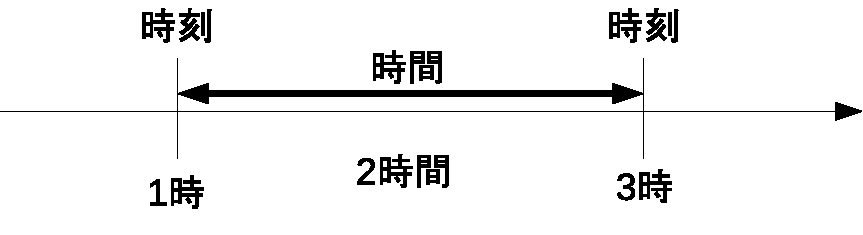
\includegraphics[keepaspectratio, width=7.2cm,height=3.6cm,clip]{jikoku-to-jikan.pdf}
                        \caption{時間と時刻}
                        \label{fig:jikoku-to-jikan}
                    \end{center}
                \end{figure}

                例えば,「1時から3時までの時間は2時間である.」という主張をするとき,
                この“2時間”が \textbf{時間} であり,1時とか3時は \textbf{時刻} である.
                時刻は幅がなく,時間を直線で表現にしたときには,点で表現される.
                それに対して,時間はある時刻と別の時刻の間の間隔である.

                勘違いを起こしがちなことがある.それは,
                すべての時刻を集めたものが時間である,という考えである.
                しかし,これは間違いだ.
                時間は数直線で表すことができ,よく,\textbf{時間軸} と
                いう言葉で表現される.時刻とは,時間軸の一点を表す語彙であるが,
                その一点には幅はない.つまり,時刻の時間は0である.0をいくらたくさん
                足しあわせたところで,結果は0であることは言うまでもない.
            \end{memo}

            \begin{memo}{飛ぶ矢のパラドクス}
                エレアのゼノン
                    \footnote{
                        $Z\eta \nu \omega \nu$(B.C.490 -- B.C.430, 古代ギリシア):
                        ギリシャ文字をそのままアルファベットに変換すると「Zhenon」.
                        しかし,英語表記で「Zeno」(ラテン語,フランス語でも同じ)で,
                        ドイツ語表記では「Zenon」と表される
                        (ドイツ語の場合,「ツェノン」と発音するのかな).
                        「エレアのゼノン」とも言われる.古代ギリシャ人.
                        ちなみに,「キプロスのゼノン」と呼ばれる,同名の人物がいるが,
                        その人とは別人.「エレアのゼノン」と書いたのも,それと区別するため.
                        キプロスのゼノンも,大哲学者であり,
                        ストア派と言われる禁欲的な態度や特を重んじる思想や態度を唱えた.
                    }
                は,次の4つのパラドクスを考えだしたことで,有名な人物である.
                    \begin{enumerate}
                        \item 二分割のパラドクス
                        \item アキレスと亀のパラドクス
                        \item 飛ぶ矢のパラドクス
                        \item 競技場のパラドクス
                    \end{enumerate}
                この内,3番目の「飛ぶ矢のパラドクス」が時間に関するパラドクスである.
                このパラドクスは,次のようなものである.動いている物体といえども,ある瞬間
                には,定まった1つの位置に位置しているはずである(写真をとるとその一点に位置している).
                定まった位置に存在するということは,静止しているのと同じ.ということは,
                動いうている物体は,瞬間的には静止しているということなる.つまり,動いている物体は,
                すべての瞬間で静止状態にあるということになる.明らかに,矛盾だ.この矛盾を
                「飛ぶ矢のパラドクス」という.
            \end{memo}

            \begin{memo}{時間とは何か}
                時間とは,一体,どこから生じているのか.
                いや,言い方を変えよう.なぜ私には時間という感覚があるのか.
                人間の知覚は五つあり,五感といわれる.
                それは,視覚,聴覚,嗅覚,触覚,味覚
                であるが,どれも直接的に時間を感じ取る器官ではない.
                それもそのはずで,「時間」という概念は外から与えられるもの
                ではなく,頭の中で作られるものだからだ.物の変化を感じ取るとき,
                頭の中で時間という感覚が生まれるのだ.

                自動車が走っているのを見て(視覚),時間を感じる.
                音楽を聴いているとき(聴覚),時間を感じる.
                部屋に芳香剤を置いて,周囲の匂いの変化を感じ,時間を感じる.
                その他いろいろ.しかし,時間という感覚を作り出すには,五感だけ
                とは限らない.考えるという行為自身が,時間概念を作り出す.

                時間は温度などのように,人間が感じる二次的な概念なのだろうか
                    \footnote{
                        今の物理学では,温度は多数の分子の運動で説明される(気体分子運動論).
                        温度は物理的な存在ではなく,分子集団の運動の激しさで説明される.
                        温度が高いとは,分子集団の持つ運動エネルギーの平均が高いということである.
                        逆に温度が低いとは,分子集団の持つ運動エネルギーの平均が低いことなのだ.
                        温度の本質は,分子集団の持つ運動エネルギーの平均値である.
                        人間が感じる温度とは,この分子の集団の運動をマクロで見た場合に生じる,
                        二次的な概念なのだ.
                    }.
                人間が勝手に時間という概念を作り出しているだけなのか.もしそうだとしたら,
                時間というパラメータのない物理理論が作れるはずである.現在の物理学において,
                時間という概念は問答無用に押し付けられる,基本パラメータである.基本パラメータ
                であるから,その性質は理論の内でわかるのかもしれないが,そもそも時間とは何かを
                追求することは不可能である.「時間とは何か」という問いに答えるには,時間以外の何かから
                時間が生成されることを説明しないとならない.現状の物理学では,そもそも時間ありきの
                理論であり,これを満たすことができない.
                物が変化できるのは時間があるからであり,物の変化があるから時間を感じるのだ.
                論理が循環してしまう.

                こう考えることはできないか.
               「記憶」という能力と「比較」という能力があることを仮定すると,
                物体の前の位置と後の位置を記憶し比較できる.
                比較の結果,前と後で違いを感じとることで,時間が生まれるのだ,と.
                とすると,記憶や比較とはどういう行為かという問題になってくるし,
                また,違いを感じ取るという感覚も説明してもらいたくなってくる.
                たとえ,記憶や比較につての説明があったとしても,その説明に使う概念の説明をもとめる
                ことになるだろう.結局,この論理では説明の無限後退になってしまう.

                論理を組み立てるには,初めに有無を言わさずに押し付けられる公理がその基礎に必要だ.
                ユークリッド幾何学では,点や線の存在は何の説明もなしに提示される.今の物理学も,
                点や線と同じように,時間は何の説明もなしにその存在が認められている.公理に対して,
                それはなぜ成り立つのかを問うても,答えは返ってこない.時間についても同じことだ.
                時間は物理学的な公理として導入されているので,時間と何かを物理学の中で答えることは
                不可能なのである.

                しかし,相対性理論などにより,物理現象に対する時間の性質を考えることはできる.
                つまり,観測者の運動と時空の関係を,理論的に考察することは可能ということだ.
                一方で,量子力学的視点に立つと,因果律がなくなってしまう
                    \footnote{
                        有名な光子の二重スリットの干渉実験では,光子の経路を特定(観測)する
                        ことはできず,実験結果を最もよく説明する仮説は,光子の取りうるすべての
                        経路を通ったとするのが,有力である.複数の経路を分裂せずに,1度に通ったというのだ.
                        因果律もあったものではない.あくまでも仮説なのだが,こう説明する以外に良い説明が
                        できないでいる.考えられるのは2通りだ.1)因果律という概念は人間が勝手に作り出した
                        ものだが,これは絶対に成り立っていて,まだ知らない事実がある.
                        2)因果律という感覚自体が錯覚であり,自然の本質には因果律という性質はない.
                    }.
                因果律とは,原因と結果の関係であり,現象の前後関係を示すもので,その根底には時間がある.
                要するに,量子力学的現象を考えると時間という概念が邪魔になってくるのだ.もっとはっきり言うと,
                時間の存在が否定されるかもしれないのである.
                ここを足掛かりとして時間理論を構築することが,目先の目標であろう.
                熱素(カロリック)やエーテルが否定されたように,時間の存在も否定されてしまうのだろうか.
            \end{memo}

            \begin{memo}{「今」見ている世界はいつの世界か}
                「今」という感覚は,何の根拠も必要としない,人間の持っている最も
                基本的なものだ.何の前置きもなしに使われる概念である.しかし,少し
                考えてみると,奇妙なものでもある.例えば,「今」自分が見ている世界の
                出来事は,いつ起こったのであろうか.光の速度が有限であることが疑いようの
                ない事実として受け入れられている現在,目に同時刻に入ってくる光景が,
                本当は同時に発生したものではないことを受け入れざるを得ない.例えば,
                夜空の星の光は何万年も前に発せられた光で,太陽の光は数分前のもので,
                目の前の景色からの光はほんの一瞬前に発生したものだ.何万年も前に発生した光と,
                さっき発生した光を同時に見ているということである.だから,同時に見えたから
                同時に発生したとは言えないのだ.
                    \begin{figure}[hbt]
                        \begin{center}
                            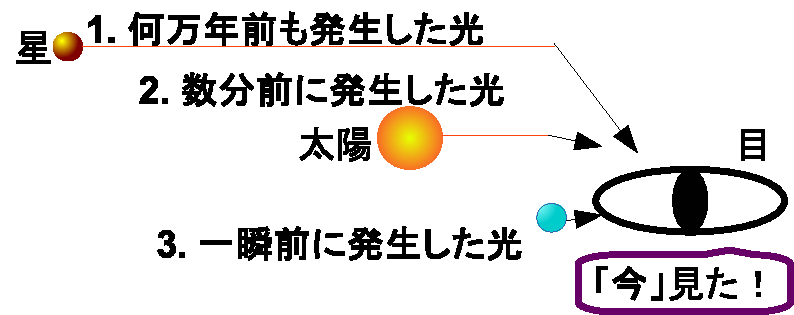
\includegraphics[keepaspectratio, width=7.2cm,height=4.8cm,clip]{star.pdf}
                            \caption{「今」見ている世界}
                            \label{fig:star}
                        \end{center}
                    \end{figure}

                今見ている現象は,いつの現象なのか.光の発生した場所により,
                観測者までの到達時間がばらつくので,観測者が同時にとらえた
                現象でも,実際に発生した時刻は異なるのである.では,
                私は今,いつの世界を見ているのか.「今」という感覚は主観的な感覚であり,
                他人と共有することはできないことは,相対性理論の主張するところであるが,
                相対論を持ち出すまでもなく,「今」という感覚は観測者個人のものでしかない.
                観測者の数だけ異なる「今」がある.

                更に言うなら,目からの視覚情報
                                        \footnote{
                                                視覚情報:目で見た目の前の光景のこと.
                                        }
                を自分が把握するには時間が必要だ.
                脳科学の教えるところによると,「見た」という感覚は,
                目からの情報を脳に伝えて,さらにその情報を脳が処理した結果である.
                ものを「見た」と感じるまでには,目からの情報を脳に伝える時間と,
                その情報を脳が処理して「見た」と感じさせるまでの時間が必要なのだ.
                ということは,今見ていると思っている目の前の光景は過去の光景ということになる.
                つまり,自分自身で感じている「今」も本当の現実世界での今ではなくなってしまう.

                「今」とは,いつのことなのだろうか.

            \end{memo}

            \begin{memo}{空間化された時間}
                時間を計るという行為は,本当に時間を計っているのだろうか.
                フランスの哲学者ベルクソン
                    \footnote{
                        Henri-Louis Bergson(1859--1941,フランス):
                        フランスの哲学者.著書($=$論文)「時間と自由」,「物質と記憶」で有名.
                    }
                は,この問に対して,否定的に答えている.時間を直接的に計れない,というのだ.
                時間を計るには,振り子(振動)にしても,アナログ時計にしても,デジタル時計にしても,
                最終的には,目に見える形で表現されたものを読み取る必要がある.目に見えるということは,
                空間的なものであり,つまり,時間の変化を空間の変化に変換して,時間の変化を捉えている
                のだ.確かに,アナログ時計で時間を計る場合,時間を示す針の位置を見ている.
                時間の変化分を,時計の針の位置の変化分に変換して,計っているのだ.
            \end{memo}

            \begin{memo}{時間の非実在性}
                時間について面白い主張がある.その主張とは,
                「時間という概念に矛盾が存在するので,時間は存在しない」というものだ.イギリスの哲学者,
                マクタガート
                    \footnote{
                        John McTaggart(1866 -- 1925, イギリス):
                        イギリスの哲学者.ラッセル(Bertrand Russell:1872--1970, イギリス)の先生でもある.
                    }
                は,1908年において,時間の非実在性 (The Unreality of Time)を唱えた.
                時間は論理的に存在しないと主張したのだ
                    \footnote{
                        「時間の非実在性(The Unreality of Time)」は,1908年に雑誌Mindで掲載された
                        論文である.もちろん,私はこの論文を読んではいない.以下の本を興味本位で
                        読んだのみである.しかし,この本は,時間の非実在性に関するマクタガートの
                        主張を噛み砕いた,丁寧な説明がなされている.一冊を割いて,この問題を
                        解説している.時間について考えるのであれば,この本を読まないわけにはいかない.
                        ただし,物理学と直接関係したような,重大な問題ではない.
                        私は,こういう考え方もありだな,という程度に捉えている.

                        (参考図書)入不二基義 [著],『時間は存在するか』,講談社現代新書,2002
                    }.
                マクタガートよれば,私達が普段使っている「時間」という概念は,少なくとも2通り存在
                する.一つ目は,時間には,過去$\cdot$現在$\cdot$未来の区別があること
                (この性質をA-系列という).二つ目は,時間の進む向きが過去から未来に向かうこと
                (この性質をB-系列という).この2つの性質を見てみると,B-系列を考えれば,時間に関して
                十分な考察ができると思われる.B-系列が,その内部にA-系列を含んでいるように見えるからだ.
                しかし,マクタガートは時間の性質を考える上ではB-系列だけを考えただけでは,
                時間を十分に捉えることができず,結局,A-系列も前提としなければならないという.
                ところが,このA-系列は,その内部に自己矛盾を含んでおり,とどのつまり,
                時間は存在しないと結論される.

                上記説明は,超概略的な説明でほとんど正確ではない.主張の雰囲気を記述しただけである.
                正確には,脚注に上げた参考図書を読んでもらいたい.
            \end{memo}

            \begin{memo}{時間が逆行しない}
                時間は逆行するか.私が今まで生きてきて,時間が逆行したことは
                ない.もっと正確に言うと,そう感じたことがない.もしかしたら,実際に
                時間は逆行しているが,私達がそう感じていないだけなのかもしれない.
                しかし,それは,私達にとって,時間の逆行したとは言えない.
                自分自身が,時間が逆行していると感じていないと,時間の逆行
                していることを観測したとはいえない.

                私たちは時間の逆行を感じることはできるのだろうか.
                もし,時間逆行を感じ取るには,何か対象となる現象が
                必要である.例えば,コップからこぼれた水がひとりでに
                コップに戻るとか,道路を行き交う車や人々が後ろ向きに
                動いているとかといった,日常で起こりうる現象と反対の
                動きをする現象を見ないといけない.また,その時に時計の針
                    \footnote{
                        デジタル時計であれば,時計に表示される,時間を示す数値.
                    }
                も逆行していることもみないといけない.ここまで見れば,
                時間が逆行しているとみなしてよいだろう.
                本当によいだろうか.周囲が偶然に逆向きに運動していただけ,
                ということは起こり得ないのだろうか.
                今の物理学では,時間の逆行を完全には否定することができない.
                つまり,厳密には,時間が逆行していることの確認は不可能なのである.
                何が足りないのか.時間の定義に何か問題があるのか.
                それとも,何か基本的なことを考え逃しているのか,見逃していいるのか.
                現在の物理学が時間の逆行を許しているにもかかわらず,なぜ,
                私たちは時間の逆行という現象を体験したことがないのだろうか.
                時間の逆行が今までに起こっていないのはなぜか.

                こう考えていても,結論を見いだせそうにない.そこで,発想を
                変えて,時間の逆行を観測したと自分が感じたと仮定してみる.
                この時の,時間逆行の観測者の状況を考えてみよう.
                時間逆行の観測者は,周囲の物体が逆向きに動いているのを
                観測している.見る物体すべてが逆に運動しているのだ.
                では,自分自身はどう観測されるのだろうか.自分自身の
                動きも逆向きに運動していないと,矛盾する.しかし,
                自分の体が逆向きに運動している状況を,観測するという
                状況を想像することは,難しい.少なくとも,それを感じている
                観測者の脳は,時間逆行していてはならない.なぜなら,
                観測者の脳が時間逆行しているとすると,記憶状態が逆向き
                に変化するということであり,記憶が消えて行くということに
                なるからである.記憶が消えてくのにもかかわらず,時間の
                逆行という,新しい現象を記憶することは不可能に思われる.
                こう考えると,時間の逆行を人間が感じ取ることは不可能なのでは
                不可能であることを,強く信じこませられる.時間の逆行を,
                本当に観測することは不可能なのだろうか.
            \end{memo}

%       %======================================================================
%       %  SubSection
%       %======================================================================
        \subsection{長さ}
            私達は「長さ」という概念は直感的に捉えることができる.
            しかし,単に「長い」だとか「短い」だとか
            といっても曖昧である.そこで,長さに基準1[m]をもうけて,
            試料の長さをこれの何倍かで表そう.ここで,
            長さの単位は[m](「メートル」と読む)で表す.
            現在,単位長さ(1[m])長さの定義は,下のように
            なされている.
            \begin{myshadebox}{単位長さ(1[m])の定義}
              1[m]は「真空中で光が 1/299792458 秒間に進む距離」と定義される.
            \end{myshadebox}

            この分数の分母の299792458という数字は光の進む速さに由来する
                \footnote{
                    光速は,$2.99792458\times10^{8}$[m/s] の速度で伝播する.
                    速度の定義は\ref{subsec:Velocity}節を参照.
                }.

            少し唐突な定義だが,今はとりあえずこれを受け止めてもらいたい.
            この定義を理解できるのは,電磁気学で電磁波について学習し終わった頃だろう.
            今すぐに理解できないからといって,あせらないでほしい.

            実は,長さの基準1[m]の定義も,時間の定義と同様に,時代とともに変化する.
            その原因は観測技術の進歩であったり,新しい理論的
            発見が為されることによる.
            従って,このような定義は,いつかは改変されるだろう.
            しかし,長さの基準が変わったからといって,物体の運動法則が変わってしまうかといえば,
            そのようなことは全く起こりえない.単位は人為的に導入するものであり,
            人間が自然を見つめるための1つの道具のようなものに過ぎない.


            現在は,特殊相対性理論が確立しており,この理論によると,
            光の進む速さはどのような速度をもった観測者から見ても一定であるということがわかる.
            これについては特殊相対性理論の部分で確認することだが,
            今はこの事実をそのまま(正しいかどうかは後まわしとして)
            受け入れえておく.このような理由(光の速さが一定であること)から,
            光を基準に取るべきではないかという,
            これまた直感によって規定された定義である.


%       %======================================================================
%       %  SubSection
%       %======================================================================
        \subsection{重さと質量}
            \begin{mycomment}
                「重さ」と「質量」は 万有引力の法則 とニュートンの運動の法則と等価原理を
                考えることによって区別されるものである.つまり,今の段階では,前提となる
                知識が不足していて,その違いを説明することができない.質量とは,運動方程式
                によって,明確に規定される量である.また,重さとは,質量の概念と,
                万有引力の法則によって,定義される量である.しかし,質量や重さのイメージ
                が説明できないわけではない.
                そこで,ここでは,その概要のみだけど,紹介しておく.
            \end{mycomment}

            万有引力の法則によると,質量をもつものは互いに引き合うという性質を
            もっている.例えば,2つのボールが存在すれば,その2つのボールは互いに引き合っている.
            実際には引き合っていないように見えるが,それは力がとても小さいからである.
            実際に引き合うことを説明するために,この2つのボール
            一方を,地球としてみる.当たり前だが,他方のボールは地球に引っ張られて地球に落ちるだろう.
            地球がボールを引っ張っているからである.また,ボールも微力ながら地球を引っ張っている.
            質量が引力を引き起こすのである.

            普段,私達の考えている「重さ」というのは,地球が物体を引っ張る力のことである.
            そこで,この「重さ」というものを基本単位にしようと思ってしまうところだが,
            そうしてしまうとある問題が生じてしまう.
            例えば,
            「地球で自身の体重を測った値」と「別の惑星で自身の体重を測った値」とを比較すると,
            全く異なった値になる.それは,地球と別の惑星の質量の差によっている.
            人間自身は全く同一人物であるから,質量は変化していないはずである.
            一人の人間が色々な惑星にいったとき,その人間を構成する原子や分子
            の量が極端に変化するようなことは理想的にはありえない
                \footnote{
                    理想的にというのは,体調の変化や精神的ストレスなどを
                    無視できるとした場合をいう.
                }.
            それにもかかわらず,
            “重さ”は測る場所によって変化する.従って,重さを基準とすることはできない.
            重さを基準として扱うとなると,いちいち“どこで測ったか”ということを問題に
            しなければならなくなってしまう.

            重さに対して,質量は場所によって変化することない.そこで,重さの変わりに,
            質量を基本単位として
            扱うのである.基準は現在も「キログラム原器」を用いている.単位を [kg] で表現する.
            単位の k は $10^{3}$ を意味する.
            \begin{figure}[hbt]
                \begin{center}
                    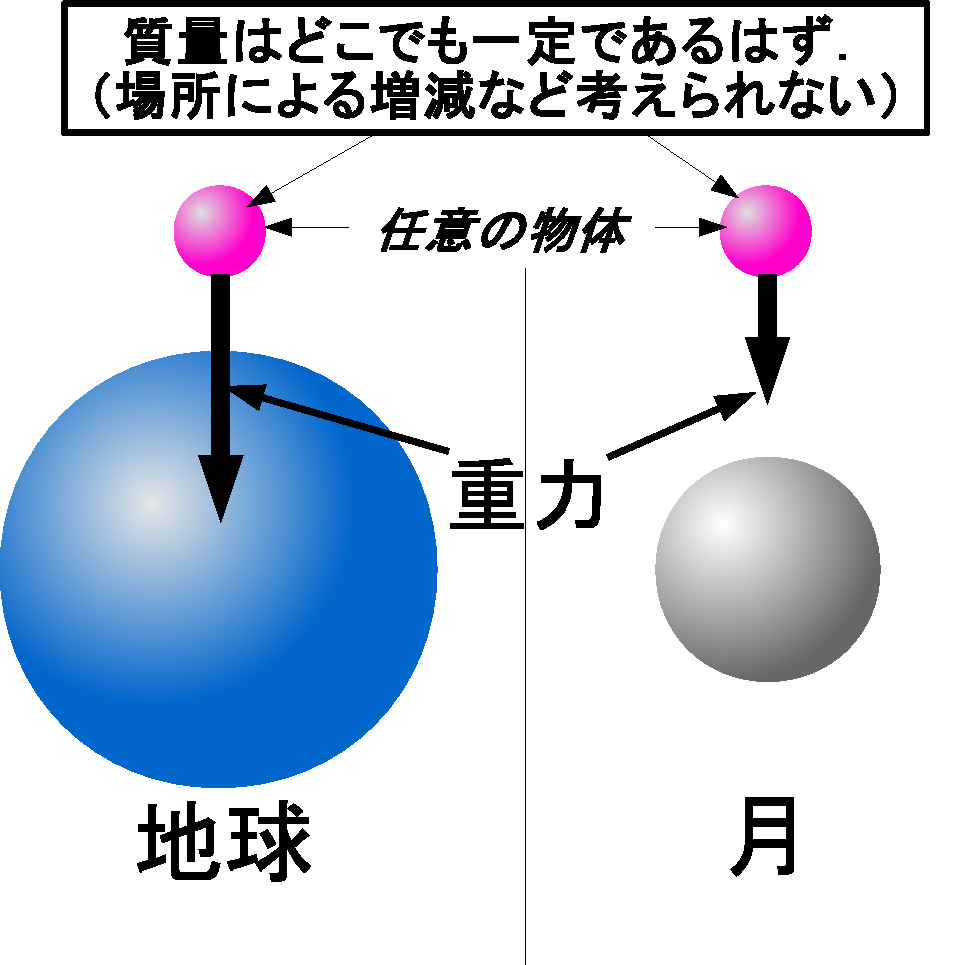
\includegraphics[keepaspectratio, width=6cm,height=6cm,clip]{mass1.pdf}
                    \caption{「質量」と「重さ」の違い}
                    \label{fig:mass1}
                \end{center}
            \end{figure}


            \begin{memo}{定量的な説明}
            \begin{mycomment}
            ここの内容は読み飛ばしてもかまわない.上の説明で,納得がいかなかった場合に読めばよい.
            詳しいことは後で考えることにして,概略を書く.
            \end{mycomment}

            物体 A が物体 B から受ける万有引力 $\bF_{\mathrm{AB}}$ は以下のように表現される.
                    \begin{align}\label{AA}
                        \bF_{\rm{AB}}
                        = -G\frac{m_{\rm{gA}}m_{\rm{gB}}}{{\left| \br_{A}
                        -\br_{B} \right|}^{2}}
                        \frac{\br_{A}-\br_{B}}{\left| \br_{A}
                        -\br_{B} \right|}
                    \end{align}
            ここに,$m_{\rm{gA}}$,$m_{\rm{gB}}$ は2つの物体 A と B のそれぞれの重力質量である.
            $\br_{A}$,$\br_{B}$は,それぞれ$m_{\rm{gA}}$と$m_{\rm{gB}}$の
            位置である.
            「重力質量」とは,万有引力を生じさせる質量のことである.$G$ は万有引力定数
            である.

            式(\ref{AA})で,物体 B を地球であるとすると,物体 A は地球から
                    \begin{align}\label{AAAAA}
                        \bF_{\rm{A-\mbox{地球}}}
                        = -G\frac{m_{\rm{gA}}m_{\rm{g\mbox{地球}}}}{{\left| \br_{A}
                        -\br_{\mbox{地球}} \right|}^{2}}
                        \frac{\br_{A}-\br_{\mbox{地球}}}{\left| \br_{A}
                        -\br_{\mbox{地球}} \right|}
                    \end{align}
            の力を受ける.
            ここで,添え字の「地球」は地球に対する質量や位置を表している.
            地球の質量 $m_{\rm{g\mbox{地球}}}$ と物体 A の位置 $\br_{A}$ は
            一定であるから,
                    \begin{align}\label{AAAAAA}
                        \textit{\textbf{g}}_{\mbox{地球}}
                        := -G\frac{m_{\rm{g\mbox{地球}}}}{{\left| \br_{A}
                        -\br_{\mbox{地球}} \right|}^{2}}
                        \frac{\br_{A}-\br_{\mbox{地球}}}{\left| \br_{A}
                        -\br_{\mbox{地球}} \right|}
                    \end{align}
            と置けば,式(\ref{AAAAA})は
                    \begin{align}\label{AAAAAAA}
                        m_{\rm{gA}}\textit{\textbf{g}}_{\mbox{地球}}=\bF_{\rm{A-\mbox{地球}}}
                    \end{align}
            と書ける.$\textit{\textbf{g}}_{\mbox{地球}}$ は \textbf{地球の重力加速度}とよばれる.

            重さとは,式(\ref{AAAAAAA})の右辺の $\bF_{\rm{A-\mbox{地球}}}$ のことであり,
            これは地球に引っ張られる力を意味している.対して,質量とは,式(\ref{AAAAAAA})の左辺の $m_{\rm{gA}}$ の
            ことである.重さが測る場所で変化するというのは,式(\ref{AAAAAA})の質量部分 $m_{\rm{g\mbox{地球}}}$ が
            惑星ごとに異なるためである.従って,重さが変化するのは $\textit{\textbf{g}}_{\mbox{地球}}$ が変化することが原因であって,
            $m_{\rm{g\mbox{地球}}}$ は何ら関係がない.質量とは,重さに含まれる力を取り除いた概念である.以上が
            重さと質量の違いである.
            \end{memo}

            \begin{memo}{お肉の重さ}
            質量と重さのもっと身近な例をあげよう.例えば,那覇で1[kg]の牛肉を
            買ったとしよう.那覇の重力加速度を9.80[m/s${}^{2}$]とすると,
                \begin{equation*}
                    \mbox{重さ} W = \mbox{質量} m_{\mathrm{i}} \times \mbox{重力加速度} \textit{\textbf{g}}
                \end{equation*}
            だから,$W=$1[kg]$\times$9.80[m/s${}^{2}$]$=$9.80[kgf] である.ここに,[kgf]は
            重さの単位で,“kilogram-force(キログラム・フォース)”という
                \footnote{
                    [kgw] と書いて,“kilogram-weight(キログラムウェイト)”ということもある.この場合は
                    日本語では「キログラム重(---ジュウ)」とよくいわれる.
                }.
            この9.80[kgf]の牛肉を,札幌にもっていくとどうなるだろうか.
            札幌の重力加速度は約9.79[m/s${}^{2}$]だから,
            つまり札幌でのこの牛肉の重さは$W=$1[kg]$\times$9.79[m/s${}^{2}$]$=$9.79[kgf] である.
            この那覇からもってきた9.80[kgf]の牛肉は
            札幌では9.79[kgf]になってしまうのである.
            別に質量が減ったのではない.那覇でも札幌でも1[kg]の牛肉である.それにもかかわらず,
            重さが0.01[kgf],つまり10[gf]も変わってしまうのである.
            実際はこのようなことが起こらないように,
            札幌と那覇でのはかりは重力加速度の違いを考慮して作られている.
            重さと質量の違いを身近に感じるのではないだろうか.
            \end{memo}


            \begin{memo}{質量は「何」からできているか}
            力学を勉強するときには,「質量」という概念は有無を言わさずに,受け入れさせられる
            はずである.しかし,この質量とはいったい何かを考えたくもなるものである.
            実際,物理学者はこの問題を考え,原子というものを発見したし,さらには,
            電子や陽子,中性子を発見している.現在では,さらに素粒子,クォークと
            どんどん詳細なことが見つかっている.では,質量は素粒子から生じているのか.
            いや,実はそうではない.素粒子は質量をもたない.では,質量はどこから生じているのか.
            この問題は「素粒子物理学」が解決してくれるものだと思う.大統一理論だとか,超ひも理論
            だとかで有名であるが,まだ完全には説明しきれていないようである
                \footnote{
                    私は啓蒙書を読んだ程度の知識なので,質量が現在どのように説明され,
                    その説明がどのように不完全なのかを握していない.
                    この理解についても,生涯の目標にしたい.
                    ただ,とても難しい数学的演算を必要とするみたいなので,これは,難しいかも...
                }.
            そんなわけで,今は質量の発生源を探ることはせず,まずは質量ありきの理論を学習しよう.

            「質量」はニュートン力学では当たり前のように使われる概念であり,物理学の基本中の基本であるが,
            その詳細は分かっていない.油断すると,質量というものは存在して当たり前だと思い,
            見過ごしてしまうかもしれない.頭の片隅に,この問題を記憶しておこう.
            \end{memo}

%       %======================================================================
%       %  SubSection
%       %======================================================================
        \subsection{基本単位のまとめ}
            以上で,基本単位の説明が終わった.
            この他にも電磁気学では電流の単位[A](アンペア)があるが,
            力学では電流という概念は扱わないのでここでは省略する.
            電磁気学の部分で電流の単位を確認することにしよう.
            さて,力学の基本単位はSI系で[s],[m],[kg]である.
            それぞれ時間,長さ,質量の単位である.
            単位の定義についてもう一度確認しておきたい.

            まず,時間の基本単位1[s]を定義した.それは「$^{133}${\rm Cs} 原子が 9192631770 回振動する時間」を1[s]とする
            というものであった.次に,この時間の単位を踏まえたうで,長さの基本単位1[m]を定義した.1[m]の定義は,
            「真空中で光が 1/299792458 秒間に進む距離」であった.
            これは光速を基とした定義である.
            そして,この2つの基本単位とは独立して,質量の基本単位1[kg]を定義した.
            といっても,質量の基本単位はキログラム原器である.
            キログラム原器の重さ1[kgf]を基にしている.


            \begin{memo}{各基本単位の関係}
            ニュートンの運動方程式は $ma=F$ である.ここに,$m$ は質量,$a$ 加速度,$F$ は力である.
            高校でも学習したように,質量 $m$ の単位は[kg],加速度 $a$ の単位は[m/s${}^{2}$]である.
            従って,力 $F$ の単位は[kg$\cdot$m/s${}^{2}$]である.力の単位としては[N](ニュートン)を
            用いることが多く,従って,
                \begin{equation*}
                    1[\mathrm{N}]=1[\mathrm{kg}\cdot\mathrm{m}/\mathrm{s}^{2}]
                \end{equation*}
            である.

            先走って書いてしまえば,電流の基本単位[A](アンペア)の定義はこの1[N]を元にして定義されている.
            どのように定義するかは電磁気学の部分で確認しよう.アンペアの定義が
            確認できたとして,物理学におけるSI系の基本単位の構成図を書いておくと,
            明瞭になると思う
                \footnote{
                    電子情報通信レクチャーシリーズ B-13,電子情報通信学会 編,
                    岩崎 俊 [著],『電磁気計測』,page 23,2006から.
                }.
                \begin{figure}[hbt]
                    \begin{center}
                        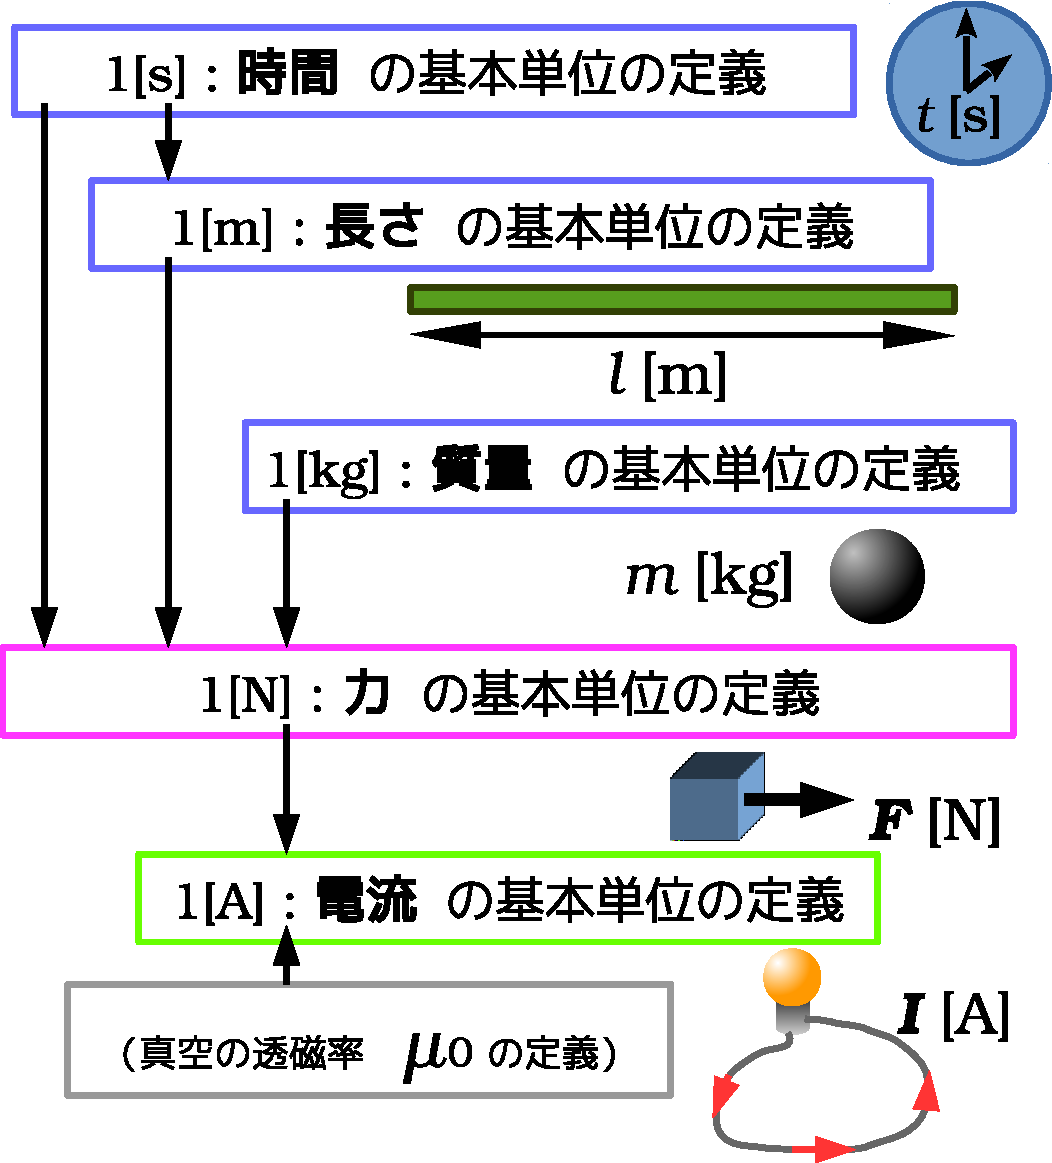
\includegraphics[keepaspectratio, width=7cm,height=8.42cm,clip]{tanni1.pdf}
                        \caption{単位の構成}
                        \label{fig:tanni1}
                    \end{center}
                \end{figure}

            最初に,原子の出す光の振動回数から,1[s]が定義される.
            そして,1[m]を光が1[s]で進む距離の1/$c$ ($c$ は光速の数値)と定義される.
            また,質量は,これらとは独立に,キログラム原器を基準に1[kg]が定義される.
            ちなみに,この1[s],1[m],1[kg]から力の単位[N](=[kg$\cdot$m/s${}^{2}$)が
            定義され,この1[N]を用いて,電流1[A]が定義される.電流の単位については
            電磁気学の項目を参照のこと.
            \end{memo}

%   %==========================================================================
%   %  Section
%   %==========================================================================
    \section{物理学における,数学の扱い方}
%       %======================================================================
%       %  SubSection
%       %======================================================================
        \subsection{道具としての数学}
            先に,物理学では数学を道具として扱うと説明した.道具として扱うとは,
            数学的厳密性を適宜無視して,数式を扱うということである.物理学の目的
            は自然現象を数式で表現することであり,重要なのは数式ではなく自然現象
            である.だから,物理学の教科書を読んでいて,数式が出てきた場合に,注
            意が必要なのである.

            数学を学習する上で大切なことのひとつに,厳密な証明の理解がある.だけ
            ど,数学を厳密に扱うとは,物理学ではあまり行わない.むしろ,厳密性を
            無視してしまっていることが多い
                \footnote{
                    例えば,テイラー(Sir Brook Taylor, 1685--1731, イギリス)展開
                    の高次の項は無視するということがある.
                }.

            物理学における数学は,あくまで道具なので,そんなに厳密に考える必要は
            ない.大切なのは,そのイメージできることである.研究者になるのでない
            限り,数学的厳密性に敏感になるよりも,数学を図形的にイメージできるよ
            うになることの方が大事である.言うまでもなく,私は研究者を目指してい
            るわけではないので,このノートでも数学的厳密性は全く気にしていない.
            このノートでは,数学を直感的に扱える程度で十分である.


%       %======================================================================
%       %  SubSection
%       %======================================================================
        \subsection{物理学の考え方}
            数学の命題や定義は絶対に不変である.後になって「間違いでした」なんて
            ことは起こらない.しかし,物理では間違いは起こる.そのたびに,修正が
            なされる.物理は実験や経験を基にしているからである.物理学ではある問
            題に対して,その原因をいろいろ仮説を立てて,実験的に仮説の正しさを確
            かめる.ここに人間の直感が介入してくる.この「人間の直感」こそが,数
            学と物理の大きな違いである.

            物理学は,感覚的なひらめきを基に構成される.だから,このひらめきが正
            しいかどうかを確認すべきだ.そのために,ひらめきを数式で表現
            して,実際に実験して検証する必要がある.物理学は,ひらめきとイメージ
            に重点が置かれているといってもよい.

            数学では考えられないことだろう.数学でも,問題を解くときにはひらめき
            はとても重要だ.そうなのだけど,物理学との違いはその検証の方法であ
            る.数学での検証は,数と論理のみで行う.そこには,実験や経験といった,
            人間の直感は含まれない.数学ではこの検証のことを「証明する」という.
            証明は数と論理で構成されいて,一度正しさが確認されれば
                \footnote{
                    (証明の)正しさの確認:論理に間違いがないことを確認すること.
                }
            後になって,間違いでしたということはない.数学に対して,物理学では,
            実験を行って,その検証を行う.実証するしかないのである.物理学では,
            証明はありえない.

            この実験が物理学の醍醐味なのだろう.自然を肌で感じ,数式で表現しさま
            ざまな予測を立てて,検証を行う.これが楽しいから,物理学があるのだ.


%       %======================================================================
%       %  SubSection
%       %======================================================================
        \subsection{物理学の数式の解釈}
            物理法則を表す数式において,等号は「\textbf{近似的に}等しい」という意味で使われる.

            数学における等号は,その右辺と左辺が全く同等であるという意味であ
            る,しかし物理では,例えば法則を数式で書き表すときに,右辺と左辺
            は本来は別々な概念であるのに,それらが等しいと書き表す.このよう
            なときに使われる等号は,“近似的”というような意味での等号である
            と考えるべきだ.この近似的という言葉も正確ではないが.なんという
            か,物理学独特の等号の使い方である.この原因は,物理学では,数学
            のような理論的厳密性よりも,\textbf{実験結果,経験が重要視される} と
            いうところにある.というのも,実験で得られる数値の桁は有限の桁で
            あり,それはもう既に近似である.だから,実験で得られる各法則も近
            似的であるし,物理の理論はこの近似の上で成立している.

            また,等号は定義するときに用いられることもある.

            もちろん,数学的な式変形のときの等号は,
            数学における等号の意味と同じである.
            これは,\textbf{恒等式} といわれる.

            \begin{memo}{恒等式}
                \textbf{恒等式} とは,変数 $x$ にどのような数を代入しても成立する
                式のことである.例えば,因数分解の公式
                    \begin{align}
                        {(x+y)}^{2}=x^{2} + 2xy + y^{2}
                    \end{align}
                がある.この式の $x$,$y$ にどのような数を代入しても,“恒に”成
                立する式である.
            \end{memo}

            \begin{memo}{方程式}
                式には,恒等式の他にも,\textbf{方程式} もある.方程式とは,例えば,
                変数 $x$ がある特別な数のときのみに成立する式のことである.その例
                として,以下の方程式を挙げよう.
                    \begin{align}
                        x^{2} - 2x + 1 = 0
                    \end{align}
                この式は,$x=1$ の場合のみにしか成立しない.このような特定の数値の
                みで成立する式が,方程式である.
            \end{memo}


%   %==========================================================================
%   %  Section
%   %==========================================================================
    \section{対称性 --- 物理学の基本要請 ---}
    \begin{mycomment}
        ここで,物理学の最も基礎となる考え方である,\textbf{対称性} について
        説明する.
        物理学には,その思想の基礎に,\textbf{対称性} という考え方を持っている.
        対称性とは,その名の通り,「どちらを見ても同じ」ということである.
        対称性という言葉は,実は,中学生の頃から使用している.
        例えば,点対称な図形は180${}^{\circ}$ 回転しても形を変えないという性質
        を持っている.また線対称な図形とは,左右あるいは上下で鏡を写したような
        形のことである.
        物理学で言う所の対称性は,点対称や線対称と同じような意味である.
        ただ違う点は,対象が図形ではなく,空間と時間に関する法則の性質である
        ことだけである.
        空間や時間の対称性とはとういうことかを,この節で説明していく.
    \end{mycomment}

%       %======================================================================
%       %  SubSection
%       %======================================================================
        \subsection{空間の対称性}
            \begin{mycomment}
                物理学では,暗黙のうちに,空間には縁がないと仮定されて理論が
                構築される.このノートでもこの原則にしたがう.具体的ないイメージ
                をしては,縁のない宇宙を想像すると良い.
                無限に広がる宇宙,あるいは,球の表面のように縁はないが有限の空間
                をイメージしてもらいたい.私達の存在するこの宇宙の具体的な形は
                不明であるが,以下の議論では,宇宙の具体的な形は問題とならない.
                将来,この宇宙の形は天文学的な観測によって明らかになることであろう.
                空間の対称性には2種類あり,次の通りである.
                    \begin{itemize}
                        \item 並進対称性
                        \item 回転対称性
                    \end{itemize}
                これらについて,以下で説明する.
            \end{mycomment}
%           %==================================================================
%           %  SubsubSection
%           %==================================================================
            \subsubsection{並進対称性}
                空間の並進対称性とは,どの方向に並行移動しようが,物理法則は
                全く変化しないということである.

                具体例で説明しよう.ある場所Aで実験していて,ある結果を得たとし
                よう.この実験結果は間違いがないものと,裏付けられたとする.こ
                の実験を別の場所Bで,全く同様の条件と方法で実験を行ったとき,
                実験結果はどうなるだろうか.全く同じ結果
                    \footnote{
                        実験誤差は当然考慮した上で.
                    }
                になるはずである.そうならなくては,その実験は正しいとは言えない.
                “どんな場所で,実験しても,実験条件と方法が同じであれば,同一の結果を得る”
                という考え方が,\textbf{空間の並進対称性} である.空間の並進対称性
                を信じているからこそ,正しい実験とその結果を受け入れることができるのである.
                ただし,並進対称性は,並進と言っているからには,実験している方向に
                関しては,していない.つまり,“同一の向きを向いて”という仮定が
                含まれているのである.

                もう一度言おう.空間の並進対称性は,場所Aで実験しても,
                場所Aから平行移動した場所Bでも,条件と方法が同じであれば,
                得られる結果も同じになるということを保証する.

                つまり,「どこで実験しても得られる結果は同じ」ということである.
                言い換えれば,\textbf{物理法則は場所により不変である}と言える.
                    \begin{myshadebox}{空間の並進対称性}
                        \textbf{空間の並進対称性} は,物理法則は場所によって不変であることを
                        主張するものである.
                    \end{myshadebox}

                    \begin{figure}[hbt]
                        \begin{center}
                            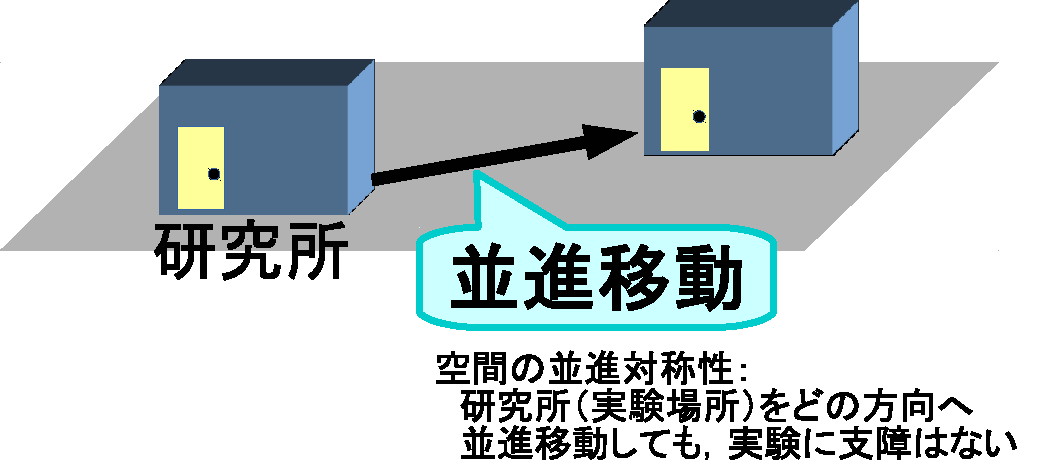
\includegraphics[keepaspectratio, width=7cm,height=3.23cm,clip]{Synmmetry_SpaceP.pdf}
                            \caption{研究所の並進移動}
                            \label{fig:Synmmetry_SpaceP}
                        \end{center}
                    \end{figure}


%           %==================================================================
%           %  SubsubSection
%           %==================================================================
            \subsubsection{回転対称性}
                並進対称性では,並進移動しても物理法則に何ら変化がないということが
                保証される.これに対して,回転対称性は,その名の通り,回転しても
                物理法則が変わらないことを保証している.ある向きで実験を行った
                とし,その後,同じ場所で別の向きで実験しても,向きを変える前と
                実験結果は同一になるということである.

                つまり,
                \textbf{空間の回転対称性} は,
                ある場所において,ある向きで実験する場合と,その場所で別の向きで
                実験する場合とで,同じ結果を得ることを保証する.

                つまり,「どの向きで実験しても,得られる結果は同じ」ということである.
                言い換えると,\textbf{物理法則は向きに対して不変である}と言える.
                    \begin{myshadebox}{空間の回転対称性}
                        \textbf{空間の回転対称性} は,物理法則が向きに対して不変である
                        ことを主張するものである.
                    \end{myshadebox}

                    \begin{figure}[hbt]
                        \begin{center}
                            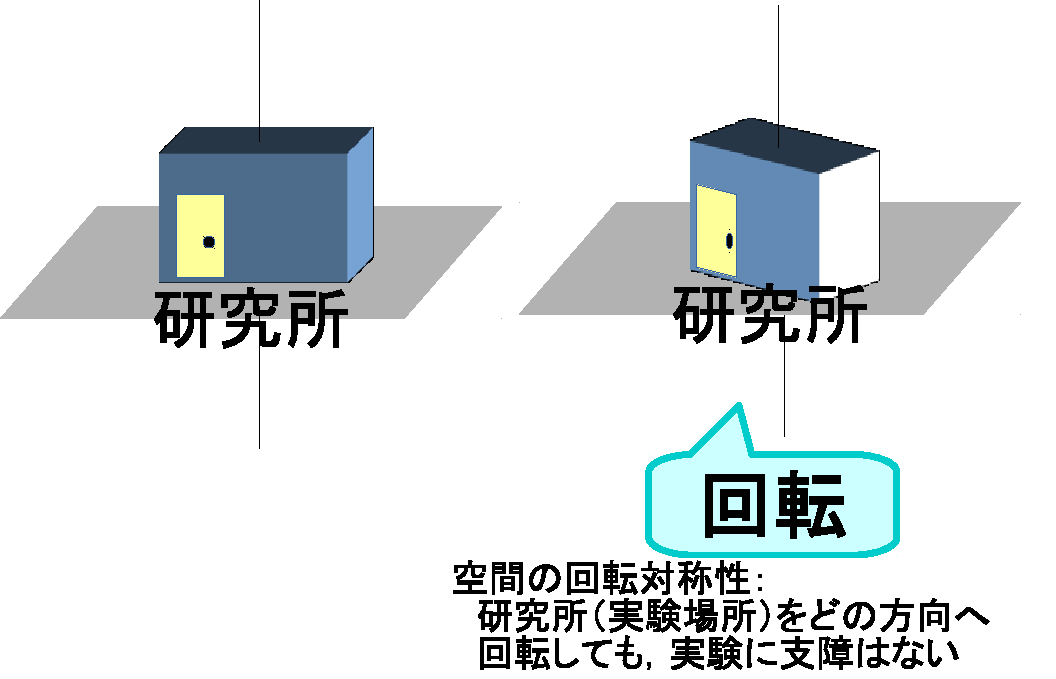
\includegraphics[keepaspectratio, width=7cm,height=4.6cm,clip]{Synmmetry_SpaceR.pdf}
                            \caption{研究所の回転}
                            \label{fig:Synmmetry_SpaceR}
                        \end{center}
                    \end{figure}


%       %======================================================================
%       %  SubSection
%       %======================================================================
        \subsection{時間の対称性}
            時間の対称性が意味するところは,とても単純で,
            物理法則が時間に対して不変であることを主張するものである.
            要するに,いつ実験しようが実験結果は変わらないということ
                \footnote{
                    もちろん,条件,方法は同じである必要がある.
                }.
            朝に実験しようが,夜中に実験しようが,実験結果は全く同じ.
            朝の実験の方が良い結果を生むということは決して無い.
                    \begin{myshadebox}{時間対称性}
                        \textbf{時間の対称性} は,物理法則が時間に対して不変である
                        ことを主張するものである.
                    \end{myshadebox}
            
            \begin{memo}{「時間の対称性」への不信感}
                時間の対称性には,少し怪しいところがある.時間には「始まり」と「終わり」
                という概念があるためである.「始まり」や「終わり」の付近では対象性がなくなる.
                時間が「始まる前」と「始まった後」では対象性があるとは言いにくいだろう.
                ただ,「時間が始まる前」というイメージに具体的に説明することもできないので
                以降では,さしあたっては,時間には「『始まり』も『終わりも』ない」と割り切って,
                この問題を脇において考察をすすめる
                    \footnote{
                        「考えられないから,考えないように目をつむるしかない」というのが
                        本音である.
                    }.
                
            \end{memo}


%       %======================================================================
%       %  SubSection
%       %======================================================================
        \subsection{対称性 --- まとめ ---}
            \textbf{対称性} という専門用語を使うと,いかにも難しい概念だと思われる
            が,その意味はとても単純であり,私たちには暗黙の了解として体に染み付い
            ているものである.対称性のおかげで,研究所を建てる場合に,場所や向きや
            時代を考えることは必要がなくなる.いや,そもそも,物理法則は場所や向き,
            時間に対して不変でなければならないという要請がなされているものである,
            といった方が正確だ.

            つまり,物理法則というからには,対称性を備えていなければならない
            のである.物理法則は,場所にかかわらず,向きにかかわらず,時間(時代)
            にかかわらず,不変性を保つものである.
                    \begin{myshadebox}{対称性}
                        \textbf{対称性} は,物理法則に要請される性質の1つである.
                        物理法則は,場所や向き,時間にかかわらず不変でなければならない,
                        という要請である.対称性により,物理法則が不変であることを
                        保証するのである.
                    \end{myshadebox}


%       %======================================================================
%       %  SubSection
%       %======================================================================
        \subsection{対称性と保存則(ネーターの定理)}
            対称性からとても大切な性質が導かれる.詳細は,解析力学を
            学習するときに確認することだが,ここでは簡単に紹介しておこう.

            唐突で申し訳ないが,下表(\ref{tab:Synmmetry_and_Conservation})をみて
            欲しい.この表を見ながら,以下の説明を読んでもらうと,幾らかは
            わかりやすいと思う.
            \begin{table}[hbt]
                \label{tab:Synmmetry_and_Conservation}
                \caption{対称性と保存則の関係}
                \begin{center}
                    \begin{tabular}{l|l}
                        \multicolumn{1}{c|}{対称性} & \multicolumn{1}{c}{保存則} \\
                        \hline\hline
                        時間の対称性 & エネルギー保存の法則 \\
                        \hline
                        空間の並進対称性 & 運動量保存の法則 \\
                        \hline
                        空間の回転対称性 & 角運動量保存の法則 \\
                        \hline
                         ゲージ対称性 & 電荷保存の法則 \\
                    \end{tabular}
                \end{center}
            \end{table}

            物理学を学習していくと,場所や向きや時間に影響されない法則を
            見つけることができる.これは \textbf{保存則} と言われる.
            例えば,中学生の頃からおなじみの,力学的エネルギー保存の法則が
            ある.これも,保存則の1つである.更にこれを一般化して,
            単に,\textbf{エネルギー保存の法則} とされるが,このエネルギー保存則
            は時間の対称性から数学的に導かれるのである
                \footnote{
                    “導けてしまう”と言ったほうが,実際的かもしれない.
                    感覚は人それぞれだけども$\cdots$.
                }.
            つまり,数学の定理
            である \textbf{ネーターの定理}に時間の対称性を照らし合わせると,
            エネルギーがいつでも一定値をとる
                \footnote{
                    いつでも一定値をとることを,\textbf{保存する} という.
                    詳細は後述する.
                }
            ことが結論されるのである.

            同様に,空間の並進対称性からは,\textbf{運動量保存の法則} が得られる.
            また,空間の回転対称性からは,\textbf{角運動量保存の法則} が得られる.
            また,ゲージ対称性からは,\textbf{電荷保存の法則} が導かれる.
            ネーターの定理の具体的な意味と保存則に関する詳細は,後に改めて考えることとし,
            ここでは紹介程度にとどめる.



\chapter{運動学}
%   %-----------------------------------------------------------------------------------------------
%   %  Input
%   %    File Name : PhysNote_CM_Kinematics.tex
%   %    説明      : 物体の運動の表現方法について,記述する
%   %-----------------------------------------------------------------------------------------------
        %===================================================================================================
%  Chapter : 運動学
%  説明    : 物体の運動の表現方法について,記述する.
%===================================================================================================
%   %======================================================================
%   % Section
%   %======================================================================
    \section{「物体の運動」の表現方法}
    \begin{mycomment}
        物理学,特に力学の主な目的は,物体の運動軌道を(数学的に)推測する
        ことにある.これから学習する力学は,スペースシャトルを地球から宇宙へ飛ばす
        際に実際に使われる理論でもある.また,アメリカの人類初の月面着陸(1969)を実現
        するにも,この力学理論が使われている
            \footnote{
                もちろん,力学だけではない.スペースシャトルや宇宙服などに使われる装置
                を作る際に用いられる理論は,
                電磁気学,物性理論,電子回路論,材料工学など様々なものが使われている.
                しかし,スペースシャトルの打ち上げ方向を決めるのには,力学理論以外には,
                何も使用していない.摩擦や,宇宙での人間の行動を考えずに,単に宇宙に飛び出して
                月に行くことだけを考えれば,250年前にニュートンが創り上げた力学理論さえあれば
                よいのである.
            }.

       物体の運動を表すには,どのような概念があるとよいのかを,この節で説明していこう.
    \end{mycomment}
%       %======================================================================
%       %  SubSection
%       %======================================================================
        \subsection{位置}
        物理学の,ここでは特にニュートン力学の重要な目的の1つに,\textbf{物体の
        運動を記述する} ことがある.記述の仕方はどのようであってもよいが,最もよ
        く表現できる道具として,数式が有力である.実際に,物理学では物体の運動を
        数式を用いて表現している.数式で表現すれば,曖昧さ無しに,誰にでも全く同
        一のイメージを与えることができる.

        物体の運動は数式を用いて行うことはわかった.では,実際に数式で表現するに
        はどうすればよいだろうか.物体の運動を記述したいのであるから,まず“物体
        がどこに存在するかを示す指標”が必要になる.この指標のことを,\textbf{位置} と
        いう.物体はいつも同じ場所に存在しているとは限らない.時々刻々と,その位
        置を変化させている物体のほうが一般的である
            \footnote{
                少なくとも,地球上の物体(私たちの体を含めて)は,時々刻々とその
                位置を変化させている.なぜなら,地球は太陽に対して公転しているの
                であるから,地球の外側(宇宙)から見れば,地球上の物体はすべて動
                いているのである.
            }.

%       %======================================================================
%       %  SubSection
%       %======================================================================
        \subsection{速度}
        物体の位置が記述できれば,それだけで物体の運動を記述でるだろうか.否,
        明らかに不可能である.物体が“どのように”運動しているかということも,
        記述すべきだ.つまり,物体の \textbf{速度} も知っておかないと
        いけない情報の1つである.速度とは,単位時間あたりに,物体がどの程度
        移動したかを示す指標である.

%       %======================================================================
%       %  SubSection
%       %======================================================================
        \subsection{加速度}
        さらに言うと,物体の速度は常に一定であることは珍しく,速度も位置と同様に,
        時々刻々と変化している方が一般的である.この速度の時間変化のことを,
        \textbf{加速度} という.

            \begin{memo}{加加速度,躍度,jerk}
                「速度」,「加速度」とくれば,「加加速度」というものも
                考えられるのではないか.実際,その通りで,
                加加速度という概念は存在している.これは,「躍度(やくど)」と
                も言われる.英単語では,jerkがそれに相当する.
                加速度が急激に変化すると,機械におおきな負担がかかること
                になる.この負担を数値で示すのが,躍度である.

                ニュートンの運動の第2法則(運動方程式)で,加速度と力は比例関係にある
                ことが分かっているので,躍度とは力の時間変化であると言い換えることも
                できる.

                なお,ニュートン力学を学ぶにあたり,躍度という概念は
                使うことはない.
            \end{memo}


%       %======================================================================
%       %  SubSection
%       %======================================================================
        \subsection{運動軌道}
        物体が,ある位置で突然と消えてしまい,次の瞬間に全く別の場所から突然現れ
        ることはない
            \footnote{
                実は,このことは後で考える \textbf{エネルギー保存の法則} に関連
                したことである.
            }.
        つまり,言い方を変えれば,時間的に位置が変化する物体について,その位置を
        時刻ごとに記録していけば,物体の \textbf{軌道} を得られるということであ
        る.実はこの物体の軌道こそが,ニュートン力学で興味ある事なのである.物体
        の運動の記述をするということは,物体の運動軌道を記述するということなので
        ある.

        では,物体の軌道を記述するには,どうしたらよいだろうか.観測できるのは,
        物体の持つ今この瞬間の性質であり,一瞬にして運動軌道を得ることはできない.
        もちろん,時間をかけて観測すればその軌道は明らかになるが,この観測でわかる
        のは,観測の対象としている物体の軌道のみであり,一般の物体についてのもので
        はない.知りたいのは,「現在の物体のもつ運動状況」から物体の軌道を推測する
        方法である.

%       %======================================================================
%       %  SubSection
%       %======================================================================
        \subsection{「運動の軌道」の表現に必要な情報}
        物体の運動を記述するということは,物体の動く道筋である
        運動の軌跡を記述するということである.そして,物体の運動の軌跡を記述する
        には,物体の位置・速度・加速度の3つが必要である.さらに,物体の位置や速
        度は時間的に変化するものなので,当然,「時刻」も必要である.この4つの要
        素を基に,数式を用いた推論を行うことで,物体の軌道を表現できる.

        ここに挙げた4つの概念,つまり,時刻・位置・速度・加速度は,数式で扱う以上,
        何らかの文字で表す必要がある.そこで,これら4つに次のように文字を割当て
        ることにする.
        \begin{myshadebox}{運動の軌跡の表現に必要なもの}
            物体の運動を数式で表現するには,次の4つの要素が必要である.
            \begin{enumerate}
                \item 時刻:$t$
                \item 位置:$\br$
                \item 速度:$\bv$
                \item 加速度:$\ba$
            \end{enumerate}
        \end{myshadebox}

        なぜ時刻を表す $t$ は普通の太さなのに,他の3つの位置 $\br$,速度 $\bv$,
        加速度 $\ba$ は太文字で表現されるかという,疑問があることと思う.これに
        ついては,この後に説明する.ここでは,このような文字が割当てられている
        ということを,知ることができれば十分である.

        ちなみに,このようなアルファベット($t$,$\br$,$\bv$,$\ba$)を割
        当てる強い理由はない.大切なのは,文字に意味を割当てるということであり,
        文字が何を意味するかではない.どのような文字を割当てても,全く同じよう
        に議論できることは明白である.ここでは,単に慣習に従って
            \footnote{
                私は単に多くの教科書で採用されている記号を流用しているに過ぎない.
                偉そうなことを書いたが,教科書でなぜこのように文字を割当ててい
                るのかは分かっていない.
            },
        時刻 $t$/位置 $\br$/速度 $\bv$/加速度 $\ba$ と割当てただけである.
        英単語を見てみると,
        時間はtime,点(位置)はrespect,速度はvelocity,加速度はacceleration
        である.その頭文字をとっているのかもしれない.

%   %==========================================================================
%   %  Section
%   %==========================================================================
    \section{位置の記述方法}
        \begin{mycomment}
            物体の存在する位置(場所)を表現することを考えてみよう.
            例えば,物体が「ここにある」とか「あそこにある」
            といっても,見る人によって見える方向は違ってくる.
            例えば,二人の人間の真中に静止している
            ボールがあるとして,そのボールは一方の人から見れば
            「右側」にあるというだろうし,
            もう一人は「左側」にあるというだろう.この場合,
            ボールが静止しているのにもかかわらず,
            二人のボールの位置に関する主張は異なっている.
            これではどうにもこうにも話が進まない.
            ここでは,この問題を解決することを考える.
        \end{mycomment}


%       %======================================================================
%       %  SubSection
%       %======================================================================
        \subsection{1次元(直線)上の位置}
                まず,最も簡単な直線上の位置を表すことを考えてみよう.
                その方法とは,
                直線の各点に数字を貼り付けて,その数字によって位置を表すというものである.
                図\ref{fig:ichi1}参照.
                このように直線上で表される位置を,\textbf{1次元} という.
                \begin{figure}[hbt]
                    \begin{center}
                        \includegraphicsdefault{ichi_1jigen.pdf}
                        \caption{1次元(直線上)での位置}
                        \label{fig:ichi1}
                    \end{center}
                \end{figure}

                位置を指定したいときは,まず,「基準」とする位置を決める必要がある.
                この基準の位置は直線上であればどこでもよいが,一度基準の位置を決めたら絶対にこの基準を
                変更してはいけない.基準はOと表記される.
                この基準から左右の直線に,数字を貼り付けていく.
                そして,直線上の物体の位置をその実数で表すのである.ここで大切なことは,
                \textbf{位置と実数が1対1に対応している} ことである
                        \footnote{
                        “1対1に対応している”ということは,『
                        位置を1つ指定したならば,それに対応する実数が1つだけに決まり,
                        逆に数字を1つ指定したならば,それに対応する位置が1つだけに定まる』ということである.
                        }.
                図\ref{fig:ichi1}で,
                点Bの位置を示すときには,$-2$といえばよい.同様に,点Aを示すには$-6$を,点Dを
                示すには$3.9$をいえばよい.つまり,「点の位置は$-2$である」とか,「点の位置は3.9である」
                とかといって,位置を表現するのである.数式的に書けば,例えば点Bの位置が$-2$であるならば
                    \begin{equation*}
                        \mbox{点{\rm B}の位置} = -2
                    \end{equation*}
                のように書けるだろう.“点の位置”という日本語ではこれから式を扱っていく上で
                不都合があるから,これを記号で表現しようと思う.すなわち
                位置を表す記号を導入し,これを $r$ と書くことにするということだ.
                すると上の「点Bの位置$=-2$」は
                    \begin{equation*}
                        r= -2
                    \end{equation*}
                のように表現できる.しかし,
                点があるのは$-2$という位置だけとは限らず,どのような場所にも
                存在する.そこで,この$-2$とか3.9とかという具体的な位置を
                表現する記号が必要となる.そこで,
                位置の代表を文字 $x$ で表現する.すると,
                \begin{align}\label{eq:rx}
                r=x
                \end{align}
                というように位置を指定できる.$r$ は単に位置を表現する記号であって,
                $x$ はその位置の“任意のどこか”を示している.$x$ には何か特定の実数を入れる余地がある.
                例えば $r=5$ と書いたならば,実数が5という位置を指定したことになる.$r=8.15$ と書いたならば,
                実数が8.15と書かれた位置を指定したことになる.このように,$x$ は何らかの数を代表していて,
                様々な実数を入れることができる.$x$ に入れる実数をいろいろ変えることができると考えて,
                $x$ のことを \textbf{変数} という.

                位置を表す実数の絶対値 $|x|$ は原点 O からの \textbf{距離} を表現
                している.このように考えれば,位置の単位として $\mathrm{[m]}$ が用いられるのも
                納得がいくだろう.
                以上が1次元(直線)上における位置の表現の仕方である.

%       %======================================================================
%       %  SubSection
%       %======================================================================
        \subsection{2次元(平面)上の位置}
                次に,平面上(2次元)の位置の表現方法を考える.位置を考えるには2つの数字を用いる必要がある.
                1次元のときは1方向だけを考えればよかったが,2次元の時には,
                2方向($x$ 方向と $y$ 方向)について考えられるからである.図\ref{fig:ichi2}参照.
                \begin{figure}[hbt]
                        \begin{center}
                        \includegraphicsdefault{ichi_2jigen.pdf}
                        \caption{2次元(平面上)での位置(2次元直交座標)}
                        \label{fig:ichi2}
                    \end{center}
                \end{figure}

                $x$ 方向と $y$ 方向の軸が直交しているので,\textbf{2次元直交座標} とよばれる.
                2次元上での位置を表現したい時には,
                数字を2つ指定する必要がある.この2つの数の代表は $x,\,y$ で表されることが多い
                \footnote{
                    その他の表現として,$x_{1},\,x_{2}$ というように書かれることもある.
                    これは数の個数が多くなった時に有効な表現である.しかしここでは,馴染みの深い $x,\,y$ で
                    書くことにしている.
                }.
                例えば,図\ref{fig:ichi2}で点Aの位置を
                示したいときは,
                \begin{align*}
                x=3\,,\,\,y=2
                \end{align*}
                と表現されるが,これでは少し見づらい.そこでここでも,
                位置を表現する記号として,$\br$ を用いる.
                ここで $r$ のように細い文字で書かないで,$\br$ のように
                太字で書いたのは,複数の数の組であることを強調したいからである.
                具体的な数の組は $(x,\,y)$ と表現され,すなわち,図\ref{fig:ichi2}の紫色の点の位置は
                \begin{align}
                \br=(3,\,2)
                \end{align}
                のように書かれる.これは,$x$ 方向が 3 という数字のところで,かつ,
                $y$ 方向が 2 という数字であるような位置を指定していることになる.
                一般には,
                \begin{align}
                \br=(x,\,y)
                \end{align}
                というように表現される.2つの変数を使って,
                任意の平面上の位置を表現するのである.

                また,図形的なイメージとして“矢印”が導入される.
                この矢印の始点は必ず原点 O にとるとし,終点は
                指定したい点にとる.
                自分が原点 O に立って,指定したい点を指で差していると考えればよい.
                この矢印のことを \textbf{ベクトル} という.もっと一般的にいえば,
                座標のように複数の数の組で表現されるものをベクトルという.
                平面上のベクトルは2つの数で表現でき,これを2次元ベクトルという.
                一般に,$n$ 個の数で表現されるベクトルを \textbf{$n$ 次元ベクトル} という.

                1つのベクトルは \textbf{向き} と \textbf{大きさ} をもつ.原点を始点にもつベクトルの向きは,
                終点の座標によって表される.例えば,原点 O を始点として,点 ($x_{1}$,\,$y_{1}$) を終点
                とするベクトル $\br$ のむきは,($x_{1}$,\,$y_{1}$) といえばよい.
                「北に何歩,東に何歩」というイメージをすればよい.
                また,ベクトルの大きさ $r$ は
                    \footnote{
                        一般にあるベクトル $\ba$ の大きさを表現したい場合は,細字にして $a$ と
                        表現されることが多い.つまり,$a:=\|\ba\|$ である.
                    }
                ,三平方の定理によって,以下のように定義される
                \begin{align}
                    r: = \|\br\| =\sqrt{{x_{1}}^{2}+{y_{1}}^{2}}.
                \end{align}
                \begin{figure}[hbt]
                        \begin{center}
                        \includegraphicslarge{vector_learge.pdf}
                        \caption{ベクトルの大きさ(2次元)}
                        \label{fig:vector_learge}
                    \end{center}
                \end{figure}

                もちろん上記は,($x_{1}$,\,$y_{1}$) に限らず,任意の点 ($x$,\,$y$) で成立するので,
                以降では,($x$,\,$y$) と書くことにしよう.
                ベクトルの向きのみを示したい場合は ($x$,\,$y$) と示す以外に, ($x/2$,\,$y/2$)とか,
                (1,\,$y/x$) とかといった表現方法も可能である.しかし,向きを指定するのにこのような方法を
                とってある記述を見たことがない.
                具体的な位置 ($x$,\,$y$) が指定されれば,この座標から大きさ $\sqrt{x^{2}+y^{2}}$ が
                計算でき,さらに向きも指定できるということから,この座標表現によって,ベクトルが記述される.
                しかし,この表現は少し長ったらしくなったり,式に複数のベクトルがあったりすると見づらくなって
                しまうので,$\br$ というような太字でベクトルを表すことが多い.


%       %======================================================================
%       %  SubSection
%       %======================================================================
        \subsection{3次元(空間)内の位置}
            ここまで説明すれば,
            3次元(空間)内の点の位置の表現の仕方は明らかだろう.
            空間には平面の場合に加えて,“高さ”があると考えられる.
            この“高さ”に対する変数を $z$ と表現する.
            そうすると,空間内の位置を表現するには $x,\,y,\,z$ の3つの変数が必要になることが
            わかる.2次元上の位置を表現するのに $\br$ という記号を
            導入したが,3次元空間以上の次元でもこの記号 $\br$ を
            使用しする.
            3次元空間内の点の位置を表現するには
            \begin{align}
            \br=(x,\,y,\,z)
            \end{align}
            と表現される.$x$ 方向と $y$ 方向と $z$ 方向の3
            つの軸が直交しているので,\textbf{3次元直交座標} という.
            これ以降,位置を考えるときは3次元空間内の位置であるとする.

            「座標を決める」ということは「$\left( x, y, z \right)$ の3つの実数の組を決める」ということである.
            この式の意味するところは,\textbf{位置と座標が1対1で対応している} ということである.
            すなわち,座標が決定されると位置が確定される.
            逆に位置が決定されると,座標が決まる
                    \footnote{ここで1つ注意しておく.
                    位置が $\br$ が $\left( x  , y ,  z \right)$ の
                    組み合わせを決めることでその位置を指定できるからといって,
                    位置 $\br$ が $\left( x  , y ,  z \right)$ の
                    関数であると考えてはいけない.なぜなら,「位置を決めること」
                    と $\left( x  , y ,  z \right)$ の組み合わせを決めることは,
                    全く同じことであるからである.} .
            \begin{figure}[hbt]
                \begin{center}
                    \includegraphicslarge{ichi_3jigen.pdf}
                    \caption{3次元直交座標}
                    \label{fig:zahyou}
                \end{center}
            \end{figure}

            一般に,点の位置 は各時刻によって異なる.しかし時刻を指定すると,1つの決まった位置を示す.
            従って,位置 は時刻の関数である.
            これを,$\textit{\textbf{r}\rm{(}$t$\rm{)}}$ と書く.
            すなわち,時刻 $t$ のときの座標を $x(t), y(t), z(t)$ と表すと,
                \begin{align}
                        \br(t) = \left( x(t), y(t), z(t) \right)
                \end{align}
            の関係を表せる.
            全ての時刻で点の位置を記録すれば,
            その点は曲線を描く.これを物体の \textbf{軌道} という.

            また,位置の図形的なイメージとして,3次元の場合も“矢印”が導入される.
            この矢印の始点は必ず原点 O にとるとし,終点は
            指定したい点にとる.
            自分が原点 O に立って,指定したい点を指で差していると考えればよいと思う.
            空間内の位置は3つの数で表現できるから,
            空間内の位置は3次元ベクトルである.

            \begin{memo}{次元とは何か}
                物理学的に考えて,線上の位置は1つの数値で表せる.
                また,面上の位置は順序付けされた二つの数値を用いて表現する
                \footnote{
                    「順序付けされた」という言い方は,次のようなことを意味する.
                        \begin{equation*}
                            \left[\, a ,\, b \, \right] \neq \left[\, b, \,a \, \right].
                        \end{equation*}
                    つまり,ベクトル $\left[\, a ,\, b \, \right]$ の成分 $a$,$b$ には
                    順番があって,この順番を入れ替えてしまうと,全く別のベクトルになって
                    しまうということである.これは $a$ と $b$ の記述順序にも意味が含まれ
                    ていることを説明してくれる.数学では,このような数の組みのことを,
                    \textbf{順序対} という言葉で表現される.ベクトルは順序対のひとつの例
                    であると考えることができよう.
                }.
                この考え方は空間内の点の表現にまで同じように拡張されて,空間
                内の点は順序付された三つの数値で表される.

                しかし,だからと言って,面上の点の位置を示すのに,絶対に二つの
                数が必要かと問われれば,必ずしもそうとは限らない.
                例えば,面を適当な大きさの区画に区切り,そのうちの任意の一箇所を原点とし
                て0という数値を割当ててみる.そして,その周りを囲む区画に対して,
                順に自然数を割当ててみよう(図\ref{fig:JigenTohaNanika_MATH}).
                こうすれば,面上の任意の区画を1つの自然数で表せる.
                この区画を無限に小さくしていくと,面上の一点を1つの数値に対応させる
                ことができそうな気がする.
                \begin{figure}[hbt]
                    \begin{center}
                        \includegraphicsdefault{JigenTohaNanika_MATH.pdf}
                        \caption{次元とは何か}
                        \label{fig:JigenTohaNanika_MATH}
                    \end{center}
                \end{figure}

                もちろん,こんなに簡単に上手くいくはずはない.だけど,ただ漠然と考
                えていただけでは,面上の点の位置を表現するには
                は二つの数値が絶対必要だと,思い込んでしまいがちである.
                「本当にそうだろうか」と常に疑いの精神を持ちながら,
                教科書を読み進めることも大切な事である
                    \footnote{
                        場合によっては,鵜呑みすることが理解への近道であることもあるが,
                        そんな場合でも,あとで確認することを怠ってはいけない.というか,
                        いつの間にかその鵜呑みが体に染み付いて,当たり前のように感じるよ
                        うになってしまい,確認することを忘れてしまってはいけない.
                    }.
            \end{memo}

            \begin{memo}{座標の張り方}
                座標を張ると言っても,いろいろな張り方がある.なので,
                同じ物体の位置を表現するにしても,その座標の張り方によって,
                その位置を示すベクトルも異なってくる
                    \footnote{
                        原点Oからみた物体の位置を示す矢印が変わってくるということ.
                    }.
                具体例を描くと,図\ref{fig:ZahyouChokkouChokusen}(A,B,C,D)の
                ようである.

                もちろん,この4つの例以外に限ったことではなく,あくまで一例である.

                図\ref{fig:ZahyouChokkouChokusen}(A)を基準に話すと,
                (B)は座標の間隔を大きめにとっているし,(C)は斜めにとっていて,
                (D)は(C)と同様だが原点の位置を変えている.

                要するに,座標の張り方は無数に存在するということである.
                だから,二人の観測者が同じ物体を見ていたとしても,座標の
                張り方が異なっていれば,当然ながら,物体の位置を表すベクトル
                が異なる.これは,一見してみると,大問題に見えるかもしれない.
                座標の張り方によって物体の位置が変わってしまうからである.
                しかし,これは別に大した問題ではないのだ.むしろ,
                この方が好都合なのである.大事なのは,“観測者に対する物体の位置”だ
                からである.いいかえれば,万人に共通の物体の位置
                    \footnote{
                        この考え方は,後に説明する \textbf{絶対空間} に関連する
                        ものである.ニュートン力学は,この絶対空間の存在は,
                        暗黙の内に前提とされている.
                    }
                を示す必要はない,ということである.知りたいのは,それぞれの観測者
                からみた物体の位置であり,すべての観測者から見た物体の位置ではない.
                そもそも,すべての観測者は同じ位置に立つことはありえないから
                    \footnote{
                        同じ場所に二人の人間が立てるはずがない.
                    },
                観測者が個々に,自身のいる場所が原点となるように座標を取ることで,
                補正が必要なくなり,計算が楽になるのだ
                    \footnote{
                        自分の位置を原点にとることで,自身の場所を意識することなく計算
                        ができるようになる.もし,万人に共通な座標を取らないとならない
                        ならば,自分のいる位置を把握し,物体と自分の相対的な位置関係も
                        考慮して計算をしないといけなくなる.
                    }.
                \begin{figure}[hbt]
                                        \centering
                    \begin{tabular}{cc}
                        \begin{minipage}{0.45\hsize}
                            \begin{center}
                                \includegraphicsdouble{ZahyouChokkouChokusen001.pdf}

                                (A)
                            \end{center}
                        \end{minipage}
                        \begin{minipage}{0.45\hsize}
                            \begin{center}
                                \includegraphicsdouble{ZahyouChokkouChokusen002.pdf}

                                (B)
                            \end{center}
                        \end{minipage}
                    \end{tabular}
                \end{figure}
                \begin{figure}[hbt]
                                        \centering
                    \begin{tabular}{cc}
                        \begin{minipage}{0.45\hsize}
                            \begin{center}
                                \includegraphicsdouble{ZahyouChokkouChokusen003.pdf}

                                (C)
                            \end{center}
                        \end{minipage}
                        \begin{minipage}{0.45\hsize}
                            \begin{center}
                                \includegraphicsdouble{ZahyouChokkouChokusen004.pdf}

                                (D)
                            \end{center}
                        \end{minipage}
                    \end{tabular}
                                \caption{座標の張り方}
                                \label{fig:ZahyouChokkouChokusen}
                \end{figure}

                しかし,いいことばかりではない.二人の観測者間で,同じ物体の位置
                が異なるため,互いに相手の目線に立ちたい場合には,位置ベクトルに
                変換を施さないといけない.
                といっても,難しい変換をするのではなく,単に,
                自分から見た相手の位置 $\bV$ を,相手から見た物体の位置 $\bU$ に
                加えてやらないといけないということ.すると,$\bW(=\bV+\bU)$ により,
                他の観測者からみた物体の位置を把握できるようになる(図\ref{fig:SoutaiTekiIchi001}).

                まとめておこう.座標の張り方は様々であり,どう取るかは,観測者
                自身が自由に選べる.これにより,観測者は計算が楽になるように
                座標を設定できる.しかし,その欠点として,複数の観測者
                間で,物体の位置が異なっていしまう.この欠点は,座標の変換という
                手段で解決する必要がある.
                    \begin{figure}[hbt]
                        \begin{center}
                            \includegraphicsdefault{SoutaiTekiIchi001.pdf}
                            \caption{相対的な位置の関係}
                            \label{fig:SoutaiTekiIchi001}
                        \end{center}
                    \end{figure}
                \end{memo}


%   %==========================================================================
%   %  Section
%   %==========================================================================
    \section{速度・速さの表現方法}\label{subsec:Velocity}
%       %======================================================================
%       %  SubSection
%       %======================================================================
        \subsection{「速度・速さ」の表現方法}
            速さとは何か.当たり前すぎて,問うまでもないかもしれない.だけど,
            これを定量的に(数学的に)扱うために,速さという感覚を整理しておきたい.

            世の中には,いろいろな速さがある.例えば,
            人間の歩く速さ,自転車の速さ,自動車の速さ,電車の速さ,新幹線の速さ,飛行機の速さ.
            これらは,順をおっていくほど速さが増すことは,誰でも承知している.
            日常生活ではこのくらいの感覚で支障はないが,数学的に扱うには,このままでは不十分だ
                \footnote{
                    速さという概念を,こんな適当な感じだけで捉えて,自動車の
                    速度制御装置を作られているはずがない.速さを定量的に扱い
                    計算できるようにすることで,初めて速さを制御できるようになる.
                }.
            物理学は速度を数学的に扱うために,計測できる量を基に,速度
                \footnote{
                    さっきまで,「速さ」と言っていたところを,「速度」と
                    言い換えてしまった.以降では,語彙「速さ」,「速度」は
                    物理学の専門用語として扱うことにする.物理学では,
                    この2つの語彙は,それぞれ異なる意味が与えられている.
                    その違いはこの節の最後に記述した.
                }
            を定義する.速度を定義するのに必要な量は,位置と時間である.
            もっと詳しく言うと,“位置の変化量”と“位置の変化に必要とした時間”である.
            これらを用いて,速度は言葉を用いて書くと次のように定義される.
                \begin{align}
                    \mbox{速度} := \frac{\mbox{位置の変化量}}
                                       {\mbox{位置の変化に必要とした時間}}
                \end{align}

            やはり,言葉で書いたのでは見難いし,数式的に扱うこともできない
                \footnote{
                    できなくはないが,非常に面倒くさい.記述も煩雑になり,
                    読みづらい.
                }.
            なので,上の速度の定義を,文字による表現に書き換えないといけない.
            物体の運動方向は3つ(3次元)だけど,最初から3方向の速度を定義する
            には,おそらく,難しいことだろう.そこで,段階を分けて,1方向/2方向/3方向 と
            順に考えることにしよう.

            話が長くなるので,ここで一度,節を区切ろう.

        \begin{memo}{「速度」と「速さ」の使い分け}
            日常生活において,私たちは「速度」と「速さ」という2つの語彙を意識して使
            い分けることはしていない
                \footnote{
                    少なくとも,私は使い分けていない.
                }.
            しかし,物理学において,「速度」と「速さ」という言葉は意味のことのなるも
            のとして,下のように区別して使用される.
                \begin{itemize}
                    \item \textbf{速度} とは,向きを含む,ベクトルである
                    \item \textbf{速さ} とは,向きを含まない,スカラーである
                \end{itemize}

            口頭で話すときには,両者を意識せずに混同てしまいがちだが,
            大抵の場合,話の流れからどちらを意味しているかを判断できる.
            しかし,文書に著す場合には,両者を区別して記述したい.
        \end{memo}

%       %======================================================================
%       %  SubSection
%       %======================================================================
        \subsection{「変化」の数式化}
        \begin{mycomment}
            速度とは,位置の時間的な変化で表せることが分かった.
            では,変化をどのように表現すべきか.
            変化を定量的に扱えるようにするため,数式による変化の扱い方を学習する.
        \end{mycomment}
        物理学で主に行われることは,物体の構造解析と,物体の運動規則の探究である.
        物体の構造解析で今までに分かっていることは,いま私たちが目にしている物体
        は,すべて素粒子で構成されているということだ
            \footnote{
                素粒子とは何かとか,それがどうのように構成されているのか等の
                疑問は,このノート全体を通して探っていくことである.
            }.
        しかし,しばらくの間は,物体の構造ではなく,運動規則を考えていこう.
        物体の構造を解析するためには,物体の運動規則を知っている必要があるからだ
            \footnote{
                生の原子や分子は顕微鏡ですら見ることはできない.運動規則から
                推察し想像するしかないのだ.
            }.

         運動規則を定量化するには,変化を数式で表現する必要がある.
         物体の運動を調べるというとは,物体の動く軌跡を把握するということであり,
         その軌跡は物体の位置が変化することによって描かれるからだ.
                    \begin{figure}[hbt]
                        \begin{center}
                            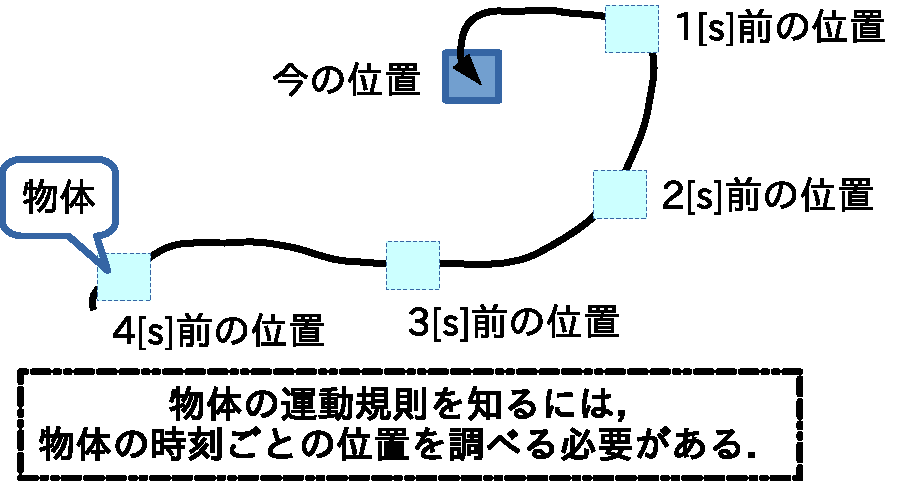
\includegraphics[keepaspectratio, width=7.2cm,height=3.72cm,clip]{henka0001.pdf}
                            \caption{軌跡$=$時刻ごとの位置の記録}
                            \label{fig:henka0001}
                        \end{center}
                    \end{figure}

%       %======================================================================
%       %  SubSection
%       %======================================================================
        \subsection{位置の時間変化の図示}
        物体の位置の時間変化を1つの図で表現する場合,
        次のように書ける.

        最初の位置を $\br_{1}$ として,次の位置 $\br_{2}$ に移動したという場面を考える.
        $\br_{1}$ から $\br_{2}$ に変化したのであるから,位置の変化分 $\br$ は
        \[
            \br = \br_{2} - \br_{1}
        \]
        とかける.
        \begin{figure}[hbt]
            \begin{center}
                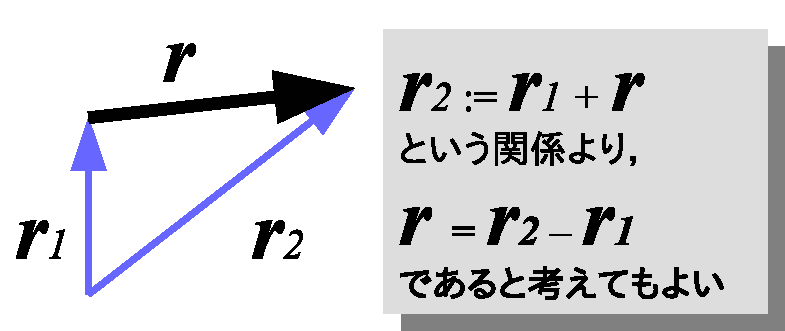
\includegraphics[keepaspectratio, width=6.2cm,height=3.2cm,clip]{ichi_henka.pdf}
                \caption{ベクトルの引き算}
                \label{fig:ichi_henka}
                \end{center}
        \end{figure}


%       %======================================================================
%       %  SubSection
%       %======================================================================
        \subsection{1次元(直線)上の速度}
                最初に,直線上を動く物体の様子について考えてみる.
                物体が直線上を運動するとき,物体は様々な速さで動くだろう.
                また,物体は直線上を右から左へ,もしくは左から右へ気まぐれに
                動くだろう.このような物体の運動を記述するにはどうすればよい
                だろうか.

                物体は直線上を動くと仮定しているので,物体は必ず直線上に存在し,$x(t)$ とい
                う1つの数で表現できる.
                物体が“動く”ということは, \textbf{時刻変化に伴って位置を変える} というこ
                とである.従って,
                時刻の変化 と 位置の変化 を考えれば物体の速さを表現できると考えられる.では,
                時刻の変化と位置の変化
                をどのように用いれば,速度を表現できるだろうか.その解決方法は,
                時刻の変化に対してどの程度の位置が変化するかという
                ことを表現すればよい.具体的に,2秒間で5[m]進む時の速さ と,
                3秒間で8[m]を進むときの速さ を考えてみよう.どちらが速いだろうか.
                これを考える場合,1秒間に対する移動距離を計算すればよい.
                2秒間で5[m]を進むのであれば,1秒間に2.5[m]進んでいて,
                3秒間で8[m]を進むのであれば,1秒間に2.6...$\cong$2.67[m]進んでいることになる.
                すなわち,3秒間で8[m]を進む方が速いと結論される.
                この具体的な計算で,距離を時間で割ることで1秒間に進む距離を計算し,
                その大きさによってどちらが速く動くかの結論を下した.
                これを一般の場合に拡張して,時間 $\Delta t$ の間に,物体
                の位置が $\Delta x$ だけ変化したとき,その速さは $\Delta x/\Delta t$ で
                表現されると言える.これ以降では速さを表現する記号として $v$ を用いることにする.
                すなわち,
                \begin{align}
                    v:=\frac{\Delta x}{\Delta t}
                \end{align}
                である.

                この式を見れば,同じ距離でも,より短い時間で
                その距離を変化するほうが速さが大きいと言える.
                また,同じ時間でもより大きな距離を
                移動したほうが早いともいえる.

                この速さの式をもう少し考察していこう.
                例えば,
                最初の状態で物体が位置 $x_{1}$ にあって,このときの時刻が $t_{1}$ であったとす
                る($x_{1}=x(t_{1})$).
                その後,物体が位置 $x_{2}$ へ動き,このときの時刻が $t_{2}$ であるとす
                る($x_{2}=x(t_{2})$).
                とすると,物体は時刻が $t_{1}$ から $t_{2}$ へ変化したとき,
                位置が $x_{1}$ から $x_{2}$ に変化したことになる.
                \begin{figure}[hbt]
                    \begin{center}
                        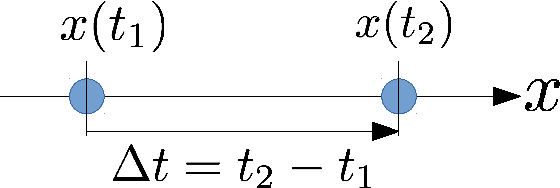
\includegraphics[keepaspectratio, width=6cm,height=3cm,clip]{sokudo1.pdf}
                    \end{center}
                    \label{fig:sokudo1}
                    \caption{速度1}
                \end{figure}

                $t_{1}$ と $t_{2}$ の時間間隔を $\Delta t$ と書いたとき,
                \begin{align}
                    \Delta t=t_{2}-t_{1}
                \end{align}
                と書ける.また同様に,
                位置も変化しているので,この位置の変化分は
                \begin{align}
                    \Delta x=x_{2}-x_{1}
                \end{align}
                と書ける.
                すると,物体の位置 $x_{1}$ から位置 $x_{2}$ へ向かうときの速さ $v$ は
                \begin{align}
                    v=\frac{\Delta x}{\Delta t}=\frac{x_{2}-x_{1}}{t_{2}-t_{1}}
                \end{align}
                となる.
                さらに,速さの式を次のように変形してみる.
                \begin{align}
                    \Delta x=v\Delta t
                \end{align}
                この式は,1次方程式の形をしている.変数は $\Delta t$ で
                あり,この変化に伴って $\Delta x$ も変化する.
                そして $v$ は変化の割合である.
                このように見れば,速さを図示して考えられる.
                1次方程式の変化の割合は,図で表現すれば,\textbf{傾き} として
                現れることになる.しかしこれには少々問題がある.
                これによって,速さ $v$ は
                わかるが,これは物体が位置 $x_{1}$ から位置 $x_{2}$ へ向かうときの
                平均的な速さでしかないのである.図\ref{fig:Sokudo2}を見てほしい.
                \begin{figure}[hbt]
                    \begin{center}
                        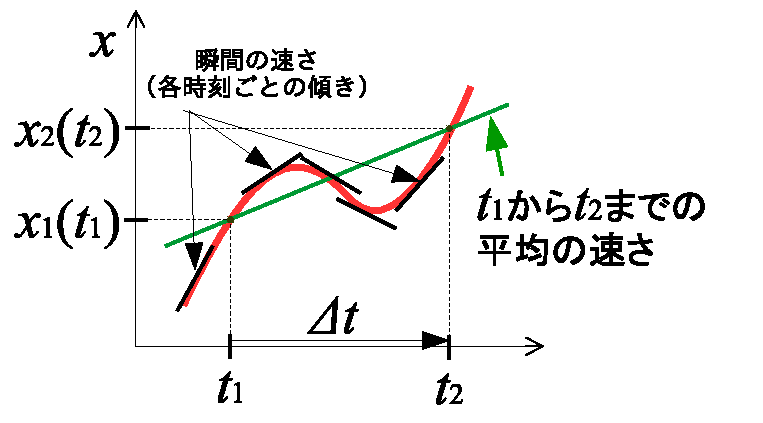
\includegraphics[keepaspectratio, width=7.2cm,height=3.88cm,clip]{Sokudo2.pdf}
                        \caption{速度2}
                        \label{fig:Sokudo2}
                    \end{center}
                \end{figure}

                実際の物体の速度は,各時刻で赤線の傾きであるのにもかかわらず,
                上の速さの式は,緑色の線の傾きというように
                みなされる.すなわち,
                位置 $x_{1}$ から位置 $x_{2}$ まで,
                速さが一定であるとみなされているのである.そのため,このままでは,
                ある特定の時刻における物体の速さが知りたいときには,
                速さの式は役に立たない.平均の速度だけしか考えることしか
                できないからである.

                そこで,次のように速さの式を
                いじってみる.例えば,時刻 $t_{1}$ を における
                物体の速度を知りたいとする.このとき,\textbf{時刻 $t_{2}$ を
                時刻 $t_{1}$ に近づけていけば,時刻 $t_{1}$ における
                物体の速度を得られる.}$\Delta t=t_{2}-t_{1}$ の関係式から,
                $t_{2}$ について解けば,
                \begin{align}
                    t_{2}=t_{1}+\Delta t
                \end{align}
                である.
                従って,時刻 $t_{2}$ を時刻 $t_{1}$ に近づけるとは,
                $\Delta t$ を0に近づけることと同じである.
                ところで,$\Delta t$ を0に近づけると,
                それに伴って位置も変化してしまう.位置の変化分は,
                $\Delta x=x_{2}-x_{1}$ であった.時刻を含めて
                詳しく書くと,
                \begin{align}
                    \Delta x=x(t_{2})-x(t_{1})
                \end{align}
                である.さらに,$t_{2}=t_{1}+\Delta t$ であるから,
                \begin{align}
                    \Delta x=x(t_{1}+\Delta t)-x(t_{1})
                \end{align}
                のように書ける.以上により,平均の速さの式は
                \begin{align}
                    v   &= \frac{\Delta x}{\Delta t}=\frac{x_{2}-x_{1}}{t_{2}-t_{1}}  \notag \\  \notag \\
                        &= \frac{x(t_{1}+\Delta t)-x_(t_{1})}{t_{1}+\Delta t-t_{1}} \notag \\  \notag \\
                        &= \frac{x(t_{1}+\Delta t)-x(t_{1})}{\Delta t}
                \end{align}
                のように変形できる.一般には,時刻 $t_{1}$ は任意の時刻で捉えることができるので,
                添え字の1をおとし,任意性を強調し,
                \begin{align}
                    v=\frac{x(t+\Delta t)-x(t)}{\Delta t}
                \end{align}
                と書ける.
                この式で,$\Delta t$ を0にもっていくのである.
                これを次のように表現する.
                \begin{align}
                    v=\lim_{\Delta t \to 0}\frac{x(t+\Delta t)-x(t)}{\Delta t}
                \end{align}
                この式の右辺を以下のように略記する.
                \begin{align}
                    \frac{\df x}{\df t}:=\lim_{\Delta t \to 0}\frac{x(t+\Delta t)-x(t)}{\Delta t}
                \end{align}
                この記号を用いて,速度は
                \begin{align}
                    v=\frac{\df x}{\df t}
                \end{align}
                のように表現する.但し注意することは,$\Delta t\not= 0$ を
                必ず満たしておくということである.

                図形的に考えると図\ref{fig:hayasa3}のようになる.
                \begin{figure}[hbt]
                    \begin{center}
                        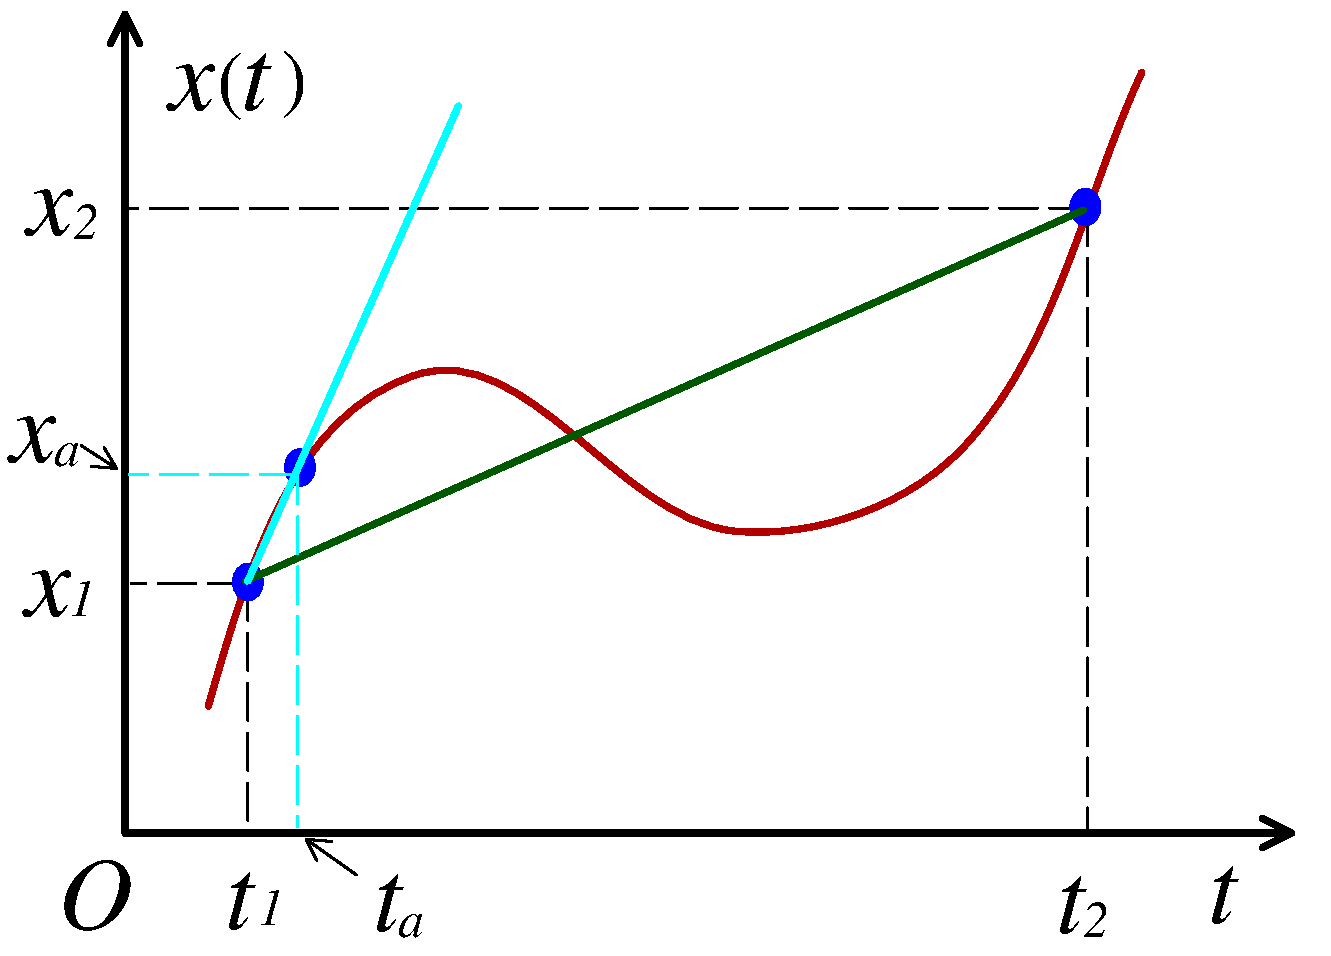
\includegraphics[keepaspectratio, width=7.2cm,height=5.73cm,clip]{hayasa3.pdf}
                        \caption{速度3}
                        \label{fig:hayasa3}
                    \end{center}
                \end{figure}

                このような図を“$x-t$ グラフ”という.
                時刻 $t_{2}$ を時刻 $t_{1}$ に
                近づけると,直線の傾き $v$ はある一定の値になる.この直線は
                水色の線で描いた.$t_{a}$ を $t_{1}$ へ
                近づいていくと,それに伴って $x_{a}$ も
                位置 $x_{1}$ へと近づいていく.但し,
                $x_{a}$ は $x_{1}$ に重ならないようにしなければならない.
                この直線が時刻 $t_{1}$ における
                瞬間の速さとなるのである.

                ここで注意しておく.それは,物体の位置と時刻の組 $(x(t),\,t)$ が
                2つ分かっていないと,速さはわからないということである.
                このことを考慮しないと,パラドクスを生んでしまうことになる.
                そのパラドクスとは,「飛ぶ矢のパラドクス」として有名である.
                次のようなものである.\\
                \begin{itembox}[l]{飛ぶ矢のパラドクス}
                動いている矢は,ある時刻を指定すれば,それに対応してある特定の
                位置で静止しているはずである.
                \end{itembox}\\

                簡単にいえば,ある時刻に撮った飛ぶ矢の写真を見ると,
                その矢は静止しているように見えるということである.
                しかし,2つの時刻で2つの位置の飛ぶ矢の写真をとれば,
                飛ぶ矢の平均の速度が求まる.もちろん,
                シャッターを押す速さが非常に速ければ,
                瞬間の速度を求められる
                \footnote{
                実際は
                そのようなことをせず,
                ビデオカメラを使うだろうが.}.

                さて,今までは速度の方向について何も考えてこなかったが,
                これは,正と負で表現できる.すなわち,左から右へ
                物体が移動するときに,物体は正方向に速度をもつ
                といい,逆に右から左に物体が移動するときには
                物体は負の向きに運動するという.


%       %======================================================================
%       %  SubSection
%       %======================================================================
        \subsection{2次元(平面)上の速度}
            2次元上,すなわち平面上における
            物体の位置は2つの方向で考える.この物体の位置は $\br=(x,\,y)$ のように
            表現される.    その速度についても2つの方向を考える必要がある.
            $x$ 方向の速度を $v_{x}$ また,$y$ 方向の速度 $v_{y}$ と
            したとき,$\bv=(v_{x},\,v_{y})$ である.
            これらはそれぞれ1次元における速度と同じように考えられて,
            \begin{align}
                v_{x}=\frac{\df x}{\df t}:=\lim_{\Delta t \to 0}\frac{x(t+\Delta t)-x(t)}{\Delta t} \notag \\
                v_{y}=\frac{\df y}{\df t}:=\lim_{\Delta t \to 0}\frac{y(t+\Delta t)-y(t)}{\Delta t}
            \end{align}
            である.

            ところで,位置が $\br=(x, y)$ と表せるので,
            速度は以下のようにも表せる.
            すなわち,
                \begin{align}
                    \bv=\left(v_{x} , v_{y}\right)
                       =\left(
                           \frac{\df x}{\df t},
                           \frac{\df y}{\df t}
                        \right)
                \end{align}
            である.


%       %======================================================================
%       %  SubSection
%       %======================================================================
        \subsection{3次元(空間)内の速度}
            3次元への拡張は容易だろう.3次元における物体の位置
            を $\br=(x,\,y,\,z)$ として,
            速度を $\bv=(v_{x}\,,\,v_{y}\,,v_{z})$ とすればよい.
            復習を兼ねてもう一度,形式的に速度について確認していく.

            時間が $t$ から $\Delta t$ だけ時間が経過したとき,
            位置は $\br(t)$ から $\br(t+\Delta t)$
            に変化する.すなわち,平均の速度 $\bar{\bv}$ は
                \begin{align}
                    \bar{\bv}
                    &= \frac{\br(t+\Delta t)-\br(t)}{t+\Delta t -t} \notag \\
                    &= \frac{\br(t+\Delta t)-\br(t)}{\Delta t }
                \end{align}
            である.知りたいのは「瞬間の速度」である.
            「瞬間の速度」を考えるために $\Delta t$ を0近づける.すると,
                \begin{align}
                    \bv
                    = \lim_{\Delta t \to \infty}\frac{\br(t+\Delta t)
                    -\br(t)}{\Delta t} \notag \\
                \end{align}
            となる.従って,
                \begin{align}
                    \bv=\frac{\df \br}{\df t}
                \end{align}
            である.これが \textbf{瞬間の速度} である.速度の単位は,[m/s] である.

            ところで,位置が $\br=(x, y, z)$ と表せるので,
            速度は以下のようにも表せる.
            すなわち,
                \begin{align}
                    \bv=\left(v_{x} , v_{y} , v_{z}\right)
                       =\left(
                           \frac{\df x}{\df t},
                           \frac{\df y}{\df t},
                           \frac{\df z}{\df t}
                        \right)
                \end{align}
            である.

            \begin{memo}{速度のを表す他の記号}
            速度は,$\df \bv/\df t$ と表現した.しかし,これを簡略化をして,以下のように書くことも
            あるので注意すべきだ.
                \begin{align}
                    \dot{\br} := \frac{\df \textit{\textbf{}v}}{\df t}.
                \end{align}
            \end{memo}

%       %======================================================================
%       %  SubSection
%       %======================================================================
        \subsection{速度の合成}
            今,人間 $A$ が速度 $\bv_{A}$ の等速で運動をしているとする.
            このとき,$A$ は 物体が速度 $\bv_{\mbox{物体}}$ をもって運動している のを見たとする.
            自分から見た物体の速度 $\textit{\textbf{V}}$ はどのようになるかを計算する.
            これは,ガリレイの \textbf{速度の合成則} によると,
                \begin{align}
                    \textit{\textbf{V}}=\bv_{\mbox{物体}}-\bv_{A}
                \end{align}
            の関係がある.この関係は,速度のベクトル和として考えられることによる.
            このように,$A$ から見た相手の速度 $\textit{\textbf{V}}$ のことを \textbf{相対速度} という.
            自分の速度を基準に, $\bv_{A}=0$ としたとき,
             $\textit{\textbf{V}}=\bv_{\mbox{物体}}$ となる.すなわち,
             自分は静止していて,動いているのは物体である主張できる.

            逆に,別の人 $B$ が物体の上から$A$を見るときを考える.$B$ は物体と共に運動している
            ことから,$\bv_{\mbox{物体}}=0$ とみなす.従って,動いているのは,$A$ であると主張できる.
            つまり,観測者によって 観測者自身の速度 が異なるので,物体の速度は 観測者によって 異なって見えるのである.
            (ここでは,観測者の立場によって,物体が動いていたり,止まっていたりしていた.)観測者の立場によって,
            互いの速度の主張は逆である.これが相対速度といわれる理由である.
            とすると,このままでは“絶対に正しい”とできる速度が存在しないことになる.
            従って,今まで,「速度」とか「加速度」とかという言葉を使ってきたが,何に対する 速度 または 加速度 であるのかを全く
            断っていなかった.この「何に対する」の『何』にあたるものが,速度や加速度の基準である.
            \begin{figure}[hbt]
                \begin{center}
                    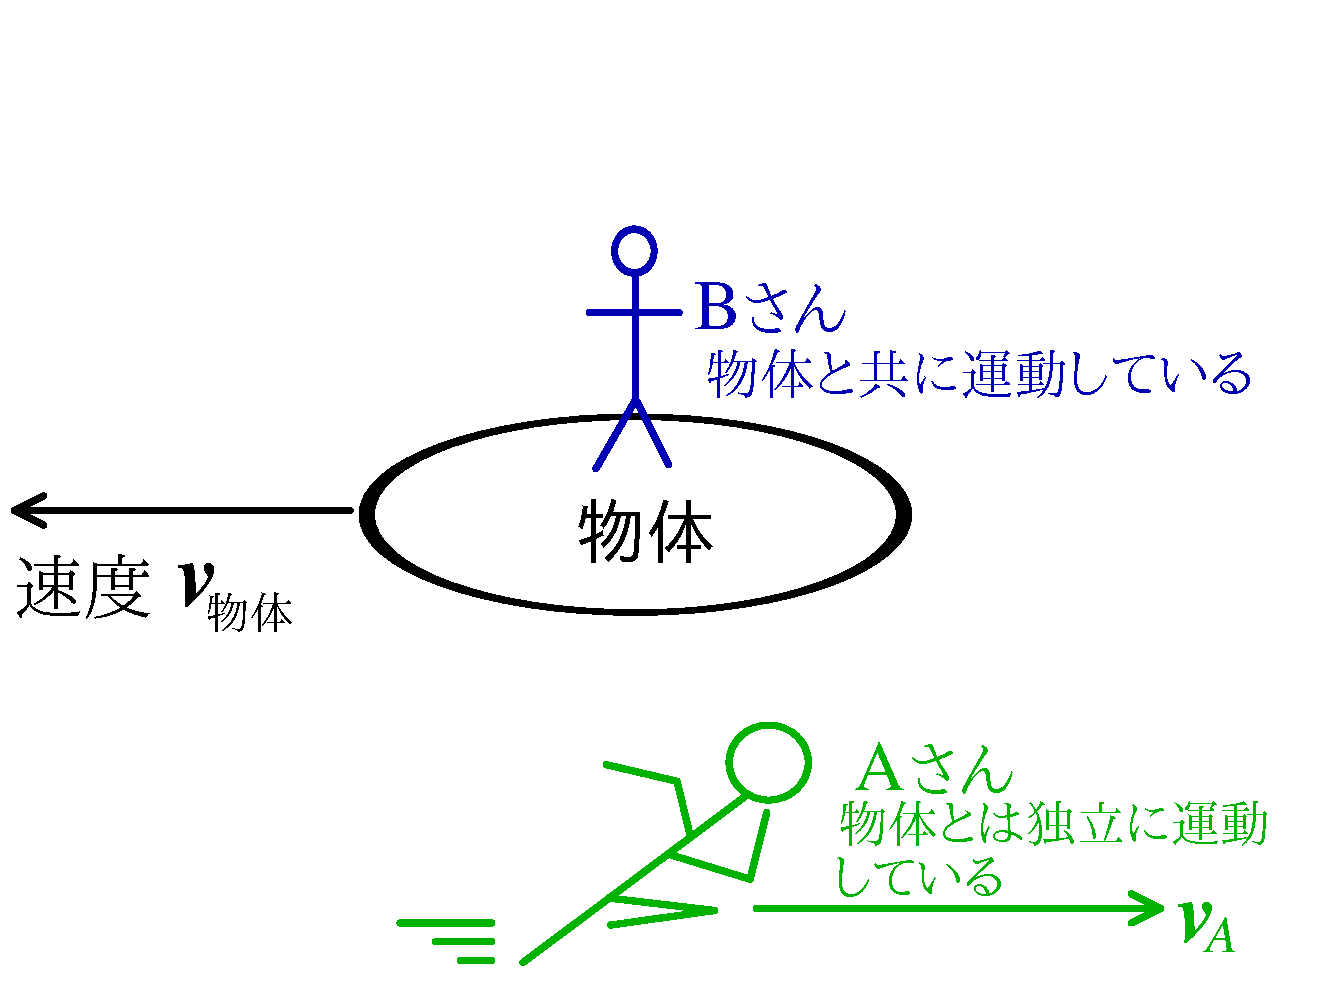
\includegraphics[keepaspectratio, width=7.2cm,height=5.92cm,clip]{soutaisokudo.pdf}
                    \caption{相対速度(Aから見た物体の速度 と Bから見た物体の速度)}
                    \label{fig:soutaisokudo}
                \end{center}
            \end{figure}

            \begin{memo}{数式と実際の現象}
                いよいよベクトルや微分,さらにはベクトルの微分と,数式が出てきは
                じめた.
                最初に戸惑うのは,数式と数式で表現されている現象との関係だろう.
                あたりまえのようだが,これについては問題を解くなりしていくしかない.
                物理学は実際の現象を数式で表す.逆にいえば物理における数式は何らかの
                物理現象を表現していると言える.式を見て,その式の内容を具体的な例で
                イメージできるように
                なるとよい.例えば,位置 $\br$ と表現されていたら,この具体的なイメ
                ージは,
                自分が原点に立っていて,その位置を指で示していることを考えればよい.
                速度 $\bv$ といわれたら,
                一定の速度で走る自転車を思い浮かべればよい.一定の速度で走るということは,
                常に時間変化 $\Delta t$ に対する自転車の変位 $\Delta\br$ が一定であることから,
                \begin{equation*}
                    \frac{\Delta \br}{\Delta t}=\mathrm{const(\mbox{一定})}=\bv
                \end{equation*}
                ということである.時間微分は,ある量(ここでは変位$\Delta \br$)時間変化に
                対する変化の割合を
                表現している.このように,式と現象が自身の中で,具体例を持って認識できる
                ようになるとよい.
            \end{memo}


%   %==========================================================================
%   %  Section
%   %==========================================================================
    \section{加速度の表現方法}
        \begin{mycomment}
            \textbf{加速度} とは,速度の時間変化具合を表す量である.
            速度を考えた時と同様に,加速度も1次元の場合から3次元の場合と,
            順を追って考えてくことにしよう.
        \end{mycomment}

%       %======================================================================
%       %  SubSection
%       %======================================================================
        \subsection{1次元(直線)上の加速度}
            一次元,つまり,直線的に運動する物体の速度 $v_{x}(t)$ は
            位置 $x(t)$ の時間変化 $\df / \df t$ として定義された.
            定義された.定義式は次の通りであった.
                \begin{align}
                    v_{x}(t) := \frac{\df x(t)}{\df t}
                              = \lim_{\Delta t \rightarrow 0}\frac{x(t+\Delta t)-x(t)}{\Delta t}.
                \end{align}

            ここでは更に,“速度の時間変化”を考える.この速度の時間変化を \textbf{加速度} と
            いう.以下に加速度を定義していこう.

            ある時刻 $t_{0}$ における物体の速度を $v_{x0}$ としたとき,
                \begin{equation*}
                    v_{x0} = v_{x}(t_{0})
                \end{equation*}
            という式が成り立つ.そして,次の時刻 $t_{1}$ における物体の速度 $v_{x1}$ は,
                \begin{equation*}
                    v_{x1} = v_{x}(t_{1})
                \end{equation*}
            と書ける.つまり,時刻 $t_{0}$ から $t_{1}$ までの間に,
            物体の速度は $v_{x0}$ から $v_{x1}$ に変化したことになる.
            時刻の変化(時間)を $\Delta t$,速度の変化を $\Delta v$ とし,
                \begin{align*}
                    \Delta t &= t_{1}  - t_{0}   \\
                    \Delta v &= v_{x1} - v_{x0}
                \end{align*}
            と置けば,加速度 $a_{x}$ は以下のように定義できる.すなわち,
                \begin{align}
                    a_{x} := \frac{\Delta v}{\Delta t}
                \end{align}
            である.これにより,加速度が速度の時間変化で定義されることが,
            示せた.

            もう少し,加速度の定義式を具体化していこう
                \footnote{
                    今まで置いた文字を展開していくことになる.効率の悪い説明だが,気にしない.
                }.
                \begin{align*}
                    a_{x} &= \frac{\Delta v}{\Delta t}                     \\
                          &= \frac{v_{x1} - v_{x0}}{\Delta t}              \\
                          &= \frac{v_{x}(t_{1}) - v_{x}(t_{0})}{\Delta t}  \\
                          &= \frac{v_{x}(t_{1}) - v_{x}(t_{0})}{\Delta t}  \\
                          &= \frac{v_{x}(t_{0}+\Delta  t) - v_{x}(t_{0})}{\Delta t}.
                \end{align*}
            ここで,$\Delta t = t_{1} - t_{0}$ から $t_{1} = t_{0}+\Delta  t$ を使った
                \footnote{
                    書くまでもないか$\cdots$.
                }.
            最後に,右辺に対して,$\Delta t \rightarrow 0$ の極限をとろう.
                \begin{align}
                    a_{x} = \lim_{\Delta t \rightarrow 0}
                            \frac{v_{x}(t_{0}+\Delta t) - v_{x}(t_{0})}{\Delta t}.
                \end{align}
            時間 $t$ による微分の記号 $\df/\df t$ を使うことで,速度が正確に定義できるようになった.
            すなわち,
                \begin{align}
                    a_{x}    :=\frac{\df v_{x}(t)}{\df t}
                              =\lim_{\Delta t \rightarrow 0}
                               \frac{v_{x}(t_{0}+\Delta t) - v_{x}(t_{0})}{\Delta t}.
                \end{align}

            更に一般化しよう.今までは,時刻 $t_{0}$ における物体の加速度を求めていたが,
            これを任意の $t$ で置き換えよう.
            そして,改めて,今度は正式に,加速度を次式で定義しよう.
                \begin{align}
                    a_{x}(t) :=\frac{\df v_{x}(t)}{\df t}
                              =\lim_{\Delta t \rightarrow 0}
                               \frac{v_{x}(t+\Delta t) - v_{x}(t)}{\Delta t}.
                \end{align}
            上式で,左辺の加速度の表現に,時刻 $t$ が独立変数であることを,
            明記するようにした.

            \begin{memo}{速度$\cdot$位置$\cdot$加速度の関係}
                速度 $v_{x}(t)$ が,$v_{x}(t) := \df x/ \df t$ と定義
                されるので,次の関係が成立している.
                \begin{align}
                    a_{x}(t) := \frac{\df v_{x}(t)}{\df t} := \frac{\df^{2} x(t)}{\df t^{2}}.
                \end{align}
                加速度の表現として,
                    \begin{equation*}
                        \frac{\df^{2} x(t)}{\df t^{2}}
                    \end{equation*}
                というものが,最もよく用いられる.

                「加速度は,位置に関する二階微分で定義される」という(見たまんまだ).
            \end{memo}

%       %======================================================================
%       %  SubSection
%       %======================================================================
        \subsection{2次元(平面)上の加速度}
            二次元の場合の加速度も,次元が増えただけで,考えることは一次元の
            場合と同じ.違いは,一次元の場合は1方向($x$ 軸)のみで考えればよ
            かったところを,二次元の場合は,2方向($x,\,y$)を考慮する点のみ.

            2つの方向を $x$ 軸,$y$ 軸とする.$x$ と $y$ 軸はそれぞれ独立だから,
            2つを別々に考えれば良い.どの方向を向いても,加速度の定義を変更する
            必要はない
                \footnote{
                    \textbf{空間の等方性} より.空間の方法性とは,
                    どの向きに運動しようが,その物体に対する
                    物理法則は不変である,という仮説のことを言う.
                }.
            つまり,1方向で考えたことが,そのまま残りの方向にも成立するということ
                \footnote{
                    してもらわないと困る.というか,成立するものとして,定義される.
                }.

            なので,上で考えた1次元の場合の式を,2方向に適用するだけで良い.
            次のように2方向の場合の加速度が定義できる.
                \begin{align}
                    \ba (t) := \frac{\df \bv(t)}{\df t}
                             = \left(
                                   \frac{\df^{2} x(t)}{\df t^{2}},\,\;
                                   \frac{\df^{2} y(t)}{\df t^{2}}
                               \right).
                \end{align}

            ただし,表記上の問題として,位置$\cdot$速度$\cdot$加速度
            をベクトル表記(太字)にした.

%       %======================================================================
%       %  SubSection
%       %======================================================================
        \subsection{3次元(空間)内の加速度}
            3次元になろうが,やることはこれまでと同じ.
            3次元空間内における加速度を $\textit{\textbf{a}}$ と表すと,
                \begin{align}
                    \textit{\textbf{a}} := \frac{\df \bv}{\df t}
                \end{align}
            である.考え方は速度のときと同じである.
            つまり,加速度とは速度の時間変化のことである.
            速度が時間の経過とともに速くなったり,逆に遅く
            なったりしたとき,
            その変化の具合が加速度である.

            また,速度の定義式から,以下のようにも加速度を表せる.
            すなわち,
                \begin{align}
                    \textit{\textbf{a}} &= \left( a_{x} , a_{y} , a_{z} \right) \notag \\
                    &= \left( \frac{\df v_{x}}{\df t} , \frac{\df v_{y}}{\df t} ,\frac{\df v_{z}}{\df t} \right)  \notag \\
                    &= \left( \frac{\df^{2}x}{\df t^{2}},  \frac{\df^{2}y}{\df t^{2}},  \frac{\df^{2}z}{\df t^{2}} \right) \notag \\
                    &= \frac{\df^{2}\br}{\df t^{2}}
                \end{align}
            とも表現できる.
            加速度が正の場合は,速度が上がっていくことを意味する.
            また,加速度が負の場合は,速度が下がっていくことを意味する.
            もちろん,加速度が 0 であれば,速度変化はないということである.

            加速度の単位は $[\rm{m/s^{2}}]$ である
                \footnote{
                    $[\rm{m/s^{2}}]$ はメートル毎秒毎秒とよむ.
                }.

            \begin{memo}{変化の記述}
                上に,「数式と物理現象は互いに関連していている」
                というようなことを書いた.そして,数式を見たときに,
                「それを現象を具体的な例で想像できることが大切である」
                とも書いた.しかし,具体的に式をイメージする方法を
                示していなかった.そこで,ここではこの例
                    \footnote{
                        当然,ここで紹介するのは,その単なる一例であり,これが全てではない.
                        むしろ,人ぞれぞれで,想像の仕方が異なっているはずである.
                        従って,想像できるようであれば,この節を読みとばしてかまわない
                        -----むしろ混乱するだろうから,読み飛ばすべきかも知れない.
                    }
                として,また,今までの復習を兼ねて,
                いまの私の考える微積分と物理現象を考えたい.


                物体は大きさをもっているが,この物体の運動を考えるときには物体の大き
                さを無視したほうが計算上都合がよい.
                物体の重心の運動を追うことで,物体の運動の軌跡を得ることができる.
                物体をこの重心部分にギュギュ!!と押しつぶして
                大きさをなくした点を考える.このような点のことを \textbf{質点} という.
                力学では,剛体の場合を除いて,物体の運動を考える
                ときは,質点の運動のことを考える.以下では,「物体」と書かれていたのなら,
                それは,特に断りのない限り,質点と同義であるとする.

                物体の運動を語るには,最初に,物体の \textbf{位置} を表現しなければならない.
                物体の位置は \textbf{座標} を用いて表現される.
                簡単のために,自身の居る点を原点 O にとろう.
                位置を表す記号として,$\br$ と表現する.つまり,物体の位置は
                \begin{equation*}
                \br =(\,x\,,\,\,y\,,\,\,z\,)
                \end{equation*}
                のように表現される
                \footnote{
                座標としては直交座標でないといけないという制約はないが,ここでは一番わか
                りやすいと思われる
                座標としてこの座標をとった.
                }.位置については,そのイメージをすることは容易だと思う.自分が原点にいて
                ,その点を指でさしている,というイメージ
                をすればよい.

                次に,物体の \textbf{速度} を考える.物体の速度とは,位置の時間変化を表す量である.
                まず,“変化”をどのように数式で表現すればよいかを考える.
                量の変化を表すには,その変化の前と後で二つの量の差を考える必要がある.量の変化は,
                \begin{equation*}
                [\mbox{量の変化分}] = [\mbox{変化後の量}] - [\mbox{変化前の量}]
                \end{equation*}
                と計算される.上の式をもう少し格好をつけて書くと,量の変化分を表すときには,
                その量を表す記号の前に $\Delta$ を
                つける.変化する量を,例えば $x$ としたとき,変化分は $\Delta x$ と表現する
                \footnote{
                $\Delta$ は,デルタ と読む.
                }
                .従って,変化前の量を $x_{\mbox{変化前}}$,
                変化後の量を $x_{\mbox{変化後}}$ と表現すれば,
                \begin{equation*}
                \Delta x = x_{\mbox{変化前}} - x_{\mbox{変化後}}
                \end{equation*}
                となる.

                また,「Aに対するB」を考えるとき,これは比で表現できて,
                \begin{equation*}
                \frac{B}{A}
                \end{equation*}
                と数式表現できる.例えば,二人の子どもに,3つのクッキーを配るとしよう.子ども一人
                に対して,
                クッキーはどれくらい与えられるかを考えれば,3/2 個であることは容易に計算される.
                この 3/2 は,
                \begin{equation*}
                    \frac{3[\mbox{個]}}{2[\mbox{人]}}
                \end{equation*}
                という意味である.式の意味は,「子ども二人に対して,クッキーが3つ」である.これは,
                子ども一人あたりのクッキーの個数でもある(3/2[個/人]).

                変化を考えるとき,基本となるのはこの引き算と割り算であり,
                後はこの組み合わせである.
                変化の基準となるものを分母にし,変化の対象となるものを分子におく.
                具体的に表現するならば,
                \begin{equation*}
                    \frac{\Delta A}{\Delta x} = \frac{A(x_{2})-A(x_{1})}{x_{2}-x_{1}}
                \end{equation*}
                のようである.$x$ の関数である $A(x)$ を考えるとき,$x$ の変化 $\Delta x$ に対
                する $A$ の変化 $\Delta A$ が
                上式で表現されている.現象の変化を表す一般的な形は,この式のようになる.


                やっと速度について考えられるが,
                速度の定義は,時間変化 $\Delta t$ の間にどの程度位置の変化 $\Delta x$ が起こるかを
                表現する.つまり,時間変化 $\Delta t$ に対する位置の変化 $\Delta x$ であるから,
                \begin{equation*}
                \frac{\Delta x}{\Delta t}
                \end{equation*}
                と表現される.
                この式は,次のように考えるとよい.まず,時間 $\Delta t$ を1秒で一定としてみよう.
                このとき,一秒で進む距離が大きければ大きいほど速度が速くなることをこの式は表現する.
                私達の経験上においても矛盾はないだろう.また,逆に,位置の変化 $\Delta x$ を1メー
                トルで一定にして
                考えてみよう.この場合,1メートルを進む時間が短ければ短いほど速度が速くなる.1メー
                トルを1秒で
                進みのと,1メートルを0.1秒で進むのでは,完全に後者の方が速い.

                実際の速度の変化は,直交座標でいうところの,$x$,$y$,$z$ の3方向で変化する.
                これは,位置が3方向であることから,当然のことである.従って,速度も3つの向きをもつ.
                つまり,
                速度もまたベクトルである.

                式で速度に意味をもたせる時には,それに対応した文字を割当てるとよい.そこで,速度
                を表現する記号として,$\bv$ を
                使うことにしよう.このノートでは,「定義する」という意味をこめて,$:=$ を使う.
                その使用方法は,例えば,記号Aに
                Bという意味をもたせたい時に,「AをBというように定義する」というとき,A$:=$Bのよ
                うに書く.今の速度の定義の場合,
                記号Aに対応するのが $\bv$ であり,意味Bに対応するのが $\Delta \br/\Delta t$ であるか
                ら,速度の定義は次のように
                書き表される.
                    \begin{align}\label{sokudonosiki_1}
                        \bv := \frac{\Delta \br}{\Delta t}.
                    \end{align}

                しかし上の式では,前の項目で定義した速度の定義と記号が異なる.
                小さい変化という意味をこめて,$\Delta$ を使っている点である.
                この記号 $\Delta$ は有限の個数の範囲でたくさん分割したときの,その1つの区間という
                イメージで使用される.
                しかし,これはあくまでも近似的な考えである.理想的には分割個数を無限大にし,分割さ
                れた区間を無限小にしたい.
                そこで,微積分という手段を使う.
                微積分を用いることで,無限小の変化を扱うことができる.有限分割から無限分割にしたの
                で,当然,
                用いる記号も
                変えないといけない.すなわち,$\Delta$ を $\df$ に変えるということである.
                    \begin{align}\label{sokudonosiki_2}
                        \bv := \frac{\df \br}{\df t}.
                    \end{align}
                式(\ref{sokudonosiki_1})と式(\ref{sokudonosiki_2})の違いは,位置の変化を有限分割に
                して表すか,
                無限分割にして表すかの違いである.速度の定義は,無限分割の概念で定義するほうが適当
                であるから,
                式(\ref{sokudonosiki_2})が正式な速度の定義になる.

                上記はベクトルで書かれているが,これは,単なる以下の式の省略である.
                        \begin{align}
                            \left(
                                v_{x} ,\,
                                v_{y} ,\,
                                v_{z}
                            \right)
                            = \left(
                                \frac{\df {r}_{x}}{\df t} ,\,
                                \frac{\df {r}_{y}}{\df t} ,\,
                                \frac{\df {r}_{z}}{\df t}
                              \right)
                        \end{align}
            \end{memo}


    \section{躍度(加加速度,jerk)}\label{seq:jerk_define}
        理論構築には直接的に関係がないためか,力学の教科書では見かけないけど,
        加加速度(jerk)についても書いておこう.
        現実的には,加速度も時間変化する.この加速度の時間変化を \textbf{加加速度} という.
        \textbf{躍度} ともいう.個人的には,躍度という方を好む
            \footnote{
                加加速度だといい間違えたと思われて誤解されそうなので.
            }.
        英語だとjerk(ジャーク).躍度は,工学的な匂いが強い.

        一応式も書いておこう.加速度がベクトルであるから,躍度もベクトルになる.
        躍度を現す記号を$\bj$としよう
            \footnote{
                jerkからとったjである.後に使う仕事の記号jとは無関係.電気数学の虚数単位とも無関係.
            }.
        定義式は以下.
            \begin{align}\label{eq:jerk_define}
                \bj &:= \frac{\df \ba}{\df t} \\
                    &=  \frac{\df }{\df t} \left(\frac{\df \bv}{\df t}\right) \notag \\
                    &=  \frac{{\df}^{2} \bv}{{\df t}^{2}} \notag \\
                    &=  \frac{{\df}^{2} }{{\df t}^{2}} \left( \frac{\df \bx}{\df t} \right) \notag \\
                    &=  \frac{{\df}^{3} \bx}{{\df t}^{3}}. \notag
            \end{align}






\chapter{3つの運動法則 と 万有引力の法則}
%   %-----------------------------------------------------------------------------------------------
%   %  Input
%   %    File Name : PhysNote_CM_LawKinemaGrav.tex
%   %    説明      : ニュートンの運動の3法則・万有引力の法則について,説明する.
%   %-----------------------------------------------------------------------------------------------
        %===================================================================================================
%  Chapter : 運動の法則と万有引力
%  説明    : ニュートンの運動の3法則・万有引力の法則について,説明する.
%===================================================================================================
\begin{mycomment}
    ニュートン力学は,4つの法則により成立している.
    4つの法則のうち,3つは物体の運動に関する法則(運動の3法則といわれる)であり,
    残りの1つは万有引力の法則である.
    物体は,この4つの法則を満たすように運動する.
    この章では,
    ニュートンの運動の3つの法則,万有引力の法則を説明していく.
\end{mycomment}
%   %==========================================================================
%   %  Section
%   %==========================================================================
    \section{運動の3法則}
%       %======================================================================
%       %  SubSection
%       %======================================================================
  \subsection{(第1法則)慣性の法則}
                力を与えられていない物体は,その動き方に変化は生じない.
                外力が加わらなければ,等速直線運動している物体は等速直線運動を続けるし,
                静止している物体は静止し続ける.
                このような性質を物体の運動の根本原因と考え,法則と捉える.
                この法則の名前を \textbf{慣性の法則} という
                \footnote{
                  「…し続ける」という性質を,\textbf{慣性} という.
                }.

                慣性の法則は実験によってのみ確かめることができ,
                どのような原理でこの法則が成立しているのかということを問題とはしない
                  \footnote{
                    問題にすることはできない,と言ったほうがよい.物理学は自然現象を論理的に説明
                    する学問である.論理的説明をするには,説明なしに受け入れなければいけない約束事
                    を設ける必要がある.これを数学では \textbf{公理} というが,物理学でこの公理
                    に対応するものが \textbf{法則} と言われるものである.
                    慣性の法則は,このような説明なしに受け入れるべき法則の1つである.
                  }.

                まとめておこう.
                \begin{myshadebox}{慣性の法則}
                    物体の運動に関する次のような性質を,\textbf{慣性の法則} という.
                    \begin{itemize}
                        \item 座標系 $S$ に対して静止している物体は,
                              外力が加わらない限り,$S$ に対して静止し続ける.
                        \item 座標系 $S$ に対して速度をもっている物体は,
                              外力が加わらない限り,$S$ に対してその速度を保ち続ける.
                    \end{itemize}
                \end{myshadebox}
                \begin{figure}[hbt]
                    \begin{center}
                        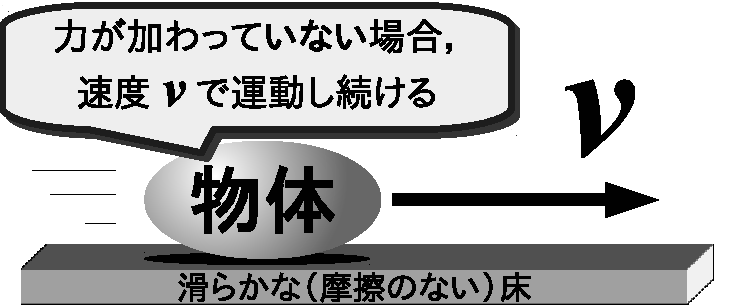
\includegraphics[keepaspectratio, width=4.8cm,height=2.0cm,clip]{kanseinohousoku.pdf}
                        \caption{慣性の法則}
                        \label{fig:kanseinohousoku}
                    \end{center}
                \end{figure}

                この法則によって,慣性系の存在が暗黙的に仮定される
                    \footnote{
                        もっとストレートに「慣性系が一つ存在する」と表せばよいのだが,どの教科書を見ても,
                        何故か,そう書かれていない.このノートもその例に従っている.
                        確かに,等速運動を続けるとか静止し続けると書いたほうが,直感的にわかりやすい.
                    }.
                「速度をもつ」とか「加速度をもつ」とかという場合,基準となる慣性系が必要だからである.
                相対速度の項目で確認したように,観測者の見る物体の速度は,
                観測者と物体間の相対速度である.すなわち,同じ物体を見ているのにもかかわらず,
                別の速度で運動している観測者にっとっては,物体は全く異なった速度として観測される.
                極端な例では,物体と同じように等速直線運動する座標系から物体を見た場合は,
                その物体は静止しているとみなされる.つまり,座標系によって物体の速度が異なってしまう.
                そこで,等速直線運動する全座標系から一つ基準となる慣性系を選び,
                この座標系を特別な座標系として扱うのが最も自然である.
                選び出された1つの座標系は速度をもっていないとみなされ
                  \footnote{
                    基準となる座標系に速度がなければ,理論的に整った(補正項のいらない)説明ができる.
                    その他の座標系は,この基準となる座標系に補正項を加えた形で表現することができる.
                  },
                これは \textbf{絶対静止系} とよばれる.

                上記の慣性の法則で言っている座標系 $S$ とは,絶対静止系のことである.
                力学は絶対静止系を,速度や加速度,力の基準として構築されている
                    \footnote{相対性理論によると,絶対静止系 $S$ の存在は否定されるが,
                        ニュートン力学を考える範囲では系 $S$ の存在を仮定したうえで成立する
                        理論である.認めてもその理論に支障はない.
                    }.

                以下では,単に速度とか加速度とかと書いた場合は,それは系 $S$ に対するもの
                であると考える.
                ちなみに,車や電車の速度の基準は,地球を基準(絶対静止系)とした場合のものである
                  \footnote{
                    地球は太陽の周りを公転しているので静止していないではないか,という反論が
                    あるかもしれないが,実際には私達は地球が静止しているように感じており,こう考えても
                    実使用上は問題はない(物理理論的には問題だが,工学的には有効な考え方である).
                    絶対静止系を任意に取れることを身近な例によって示したかったので,地球を例にした.
                  }.

                絶対静止系は等速直線運動している全座標系から任意にひとつだけ選びとった座標系であるので,
                等速度運動状態と静止状態が全く同等である.

                逆に,物体の動き方が変わった時(加速度が生じた場合)には,力が作用したと考える
                具体的には運動の第2法則(運動方程式)として記述される.
                物体に力が加わった場合,その物体は加速度が生じる.

%       %======================================================================
%       %  SubSection
%       %======================================================================
        \subsection{(第2法則)運動方程式}
                運動の第2法則は実際に動いている物体に対するものである.具体的には,
                重い物体は動かしにくく,軽い物体は動かしやすい.このようなイメージを
                式で表現する.

                物体の運動は以下の式によって記述できる.
                    \begin{align}\label{undouhouteisiki}
                        \frac{\df^{2}\br}{\df t^{2}} = k\frac{\bF}{m_{\mathrm{i}}}
                    \end{align}
                ここで,$k$は定数,$m_{\mathrm{i}}$ は \textbf{慣性質量} であり,
                $\bF$ は力 である.言葉でいうと,
                    \begin{center}
                『物体の加速度は 慣性質量に反比例し,力に比例する』
                    \end{center}
                である.これを \textbf{運動方程式} という.

                おそらく,歴史的には紆余曲折があって,最終的にこの形に落ち着いたのであろう.
                ニュートンが提示した最初の式は,微分積分学が整っておらず
                  \footnote{
                    ニュートンのこの力学の提示で,微分積分学が始まったとすれば,当然だ.
                    微分方程式という考え方はニュートンの力学以降に発展するのであり,
                    また,よりよい式表現のための記号法が整備されることになる.
                  },
                当然ながらこのような微分方程式の記述にはなっていなかったはず.
                式の形がこうなるまでの経緯は歴史的には重要かもしれないが,
                このノートでは興味のないことである.すでに数式的に整った形になっているのだから,
                これを積極的に受け入れるべきである.同じニュートンの運動法則を意味している
                のには変わりないのだから.

                運動方程式をもう少し整理し,わかりやすく書き換えよう.
                力の単位 $[\rm{N}]$ を$[\rm{N}] = [\rm{kg (m/s^{2})}]$ すると,
                定数$k$は $k=1$ になって,以下のように書ける.
                        \begin{myshadebox}{運動方程式}
                            ニュートンの運動方程式は,以下のように表現される.
                            \begin{align}\label{eq:N_eq}
                            m_{\rm{i}}\frac{\df^{2}\br}{\df t^{2}} = \bF
                            \end{align}
                        \end{myshadebox}
                        \begin{figure}[hbt]
                            \begin{center}
                                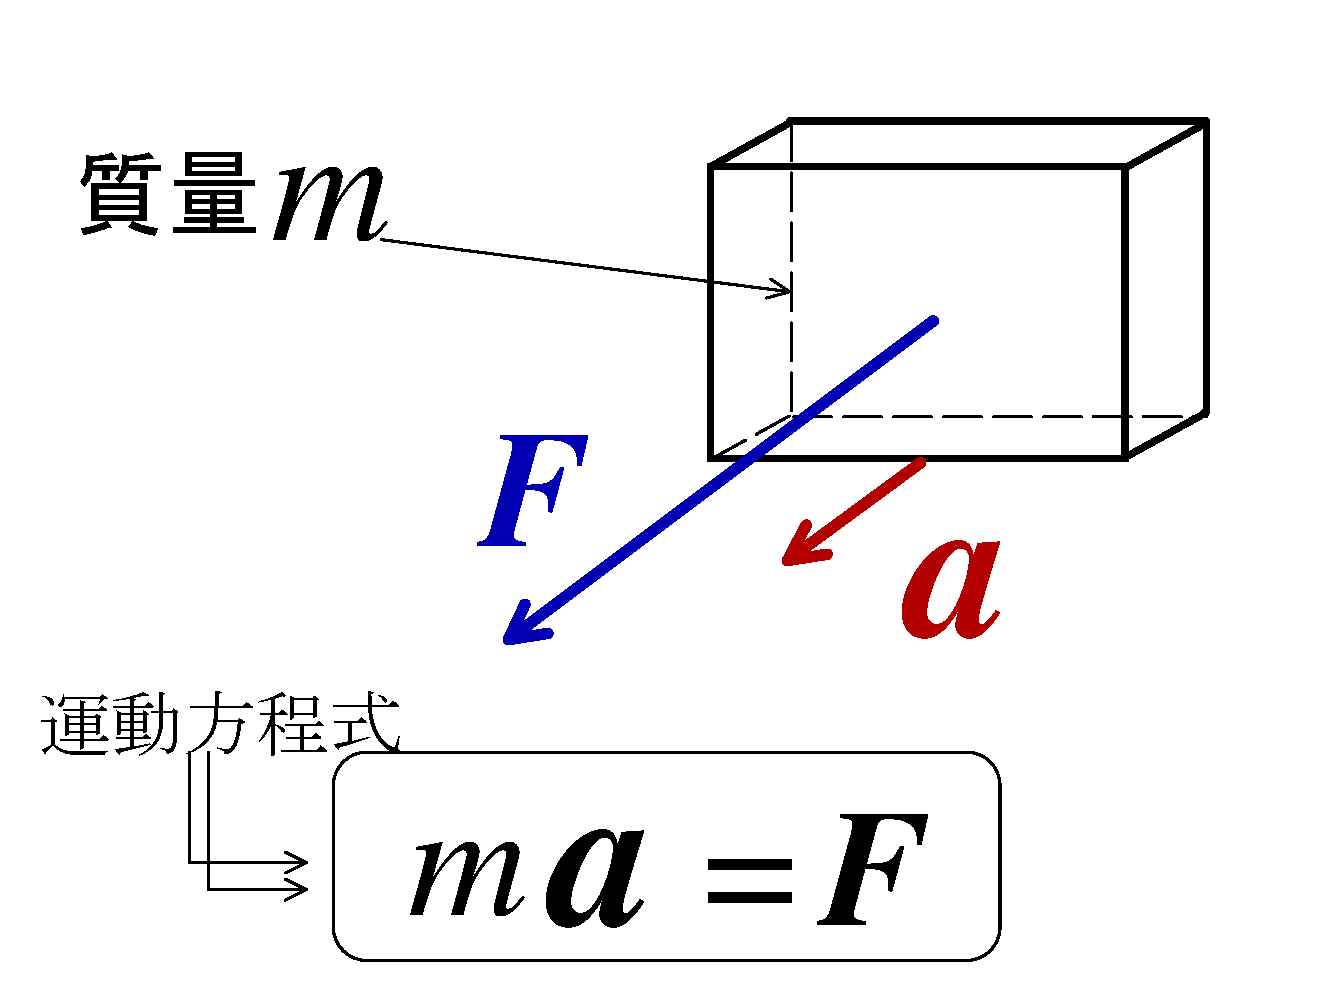
\includegraphics[keepaspectratio, width=6cm,height=6cm,clip]{ma_F.pdf}
                                \caption{運動方程式}
                                \label{fig:ma_F}
                            \end{center}
                        \end{figure}

                加速度は力に比例するので,その比例係数を慣性質量 $m_{\mathrm{i}}$ と見るのである
                    \footnote{
                        もともとあった比例定数 $k=1$ の記述は省略するが,
                        その理由が力の単位の取り方にあるということは覚えておくべきである.
                        これ以降でも様々な物理法則を表す式を見ていくが,比例定数が現れない
                        ことが多い.
                        これは理論的説明を簡潔に表現するべく,物理量の単位の定義を人為的に都合よく行っているからである.

                        単位の取り方によって,数値は変わってしまう(時には次元そのものも変わりうる)が,
                        これは物理的現象の本質ではない.物理現象を人間が説明しようとするときには,
                        ある視点からその現象を観測する必要がある.
                        観測するということは,その対象となる物理現象を偏った考えの下で見るということである.
                        こうなると当然ながら,同じ現象でも,観測方法の違いによって,測定結果がことなる場合が起こる.
                        しかし,間違いはどこにもない.どちらも正しい.同じ現象なのに,
                        測定方法によって異なる結果が出るのはおかしな気がするかもしれないが,受け入れるしかない.
                        1つの物理現象に対して,複数の物理学的説明があってもよいではないか.
                        理論は1つだけとは限らないの(人間は本当の物理法則を知ることはできない)と
                        考えるほうが健全な思考である.
                        このことは,学習を進めていくうえで忘れがちなので,ここで注意を促しておいた.
                    }.
                そうすれば「物体の質量が大きいほど,その物体に加速度をもたせるために必要な力は,
                大きくなる」と読み取れる.
                (力と加速度に具体的な数値を代入して確認してみるとよい.)
                すなわち,慣性質量は,「物体の動きにくさ」を表現していると考えられる.
                以下では,運動方程式として,式(\ref{eq:N_eq}) を用いることにする.

                運動方程式(\ref{eq:N_eq})は,慣性質量と加速度と力の3つの概念の関係を
                示しているだけであり,力の定義をなしているわけではないことに注意する.
                ここでは,とりあえず,「力」というものの存在を仮定しているのである.

                この法則で使われる等号は数学的に厳密な等号ではない.
                この法則は実験によって得られるものだからである.
                例えば,実験で加速度や慣性質量や力を
                測定するとき,必ず測定限界となる桁数が存在する.
                つまり,無限桁だけの測定はできないのだから,
                「ニュートンの運動方程式は小数点第○位の桁で正しい」としかいえない.
                すなわち,ニュートンの運動方程式(ニュートン方程式)における等号は,
                細かくいえば,近似を表すものである.
                しかし,物理では等号のようにして扱う.これによる不都合は
                ほとんどない.不都合が現れるのは量子力学や相対性理論で
                考える状況下においてである
                    \footnote{
                        相対性理論;光速に近い速度で動く物体を考える(特殊相対性理論).
                        一様でない重力が存在する空間を考える(一般相対性理論).
                        量子力学;原子レベルの大きさの粒子の運動の記述を考える.
                    }.
                そのときはニュートン方程式
                を書き換えてやればよい.このニュートン方程式は
                私達の目に見える物体の動きを
                かなりの精度で正確に記述できる方程式である.

%       %======================================================================
%       %  SubSection
%       %======================================================================
        \subsection{(第3法則)作用$\cdot$反作用の法則}
            2つの物体をもってきて,それぞれ名前をA,Bとする.
            このとき,\textbf{作用反作用の法則}とは以下のような法則のことである.
                \begin{myshadebox}{作用反作用の法則}
                    『物体Bが物体Aに力$\bF_{\rm{AB}}$を与えているとき,
                    物体Aも物体Bに$\bF_{\rm{AB}}$と大きさが同じで逆向きの力
                    $-\bF_{\rm{BA}}$を受けている』
                \end{myshadebox}
            \begin{figure}[hbt]
                \begin{center}
                    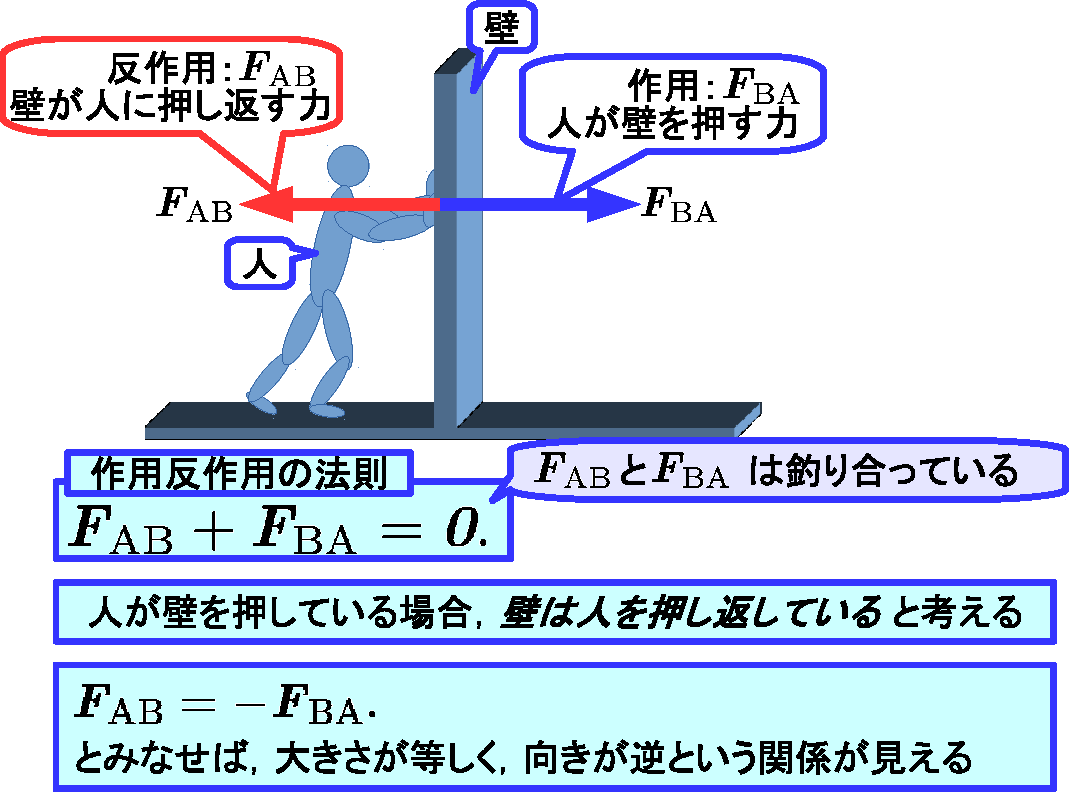
\includegraphics[keepaspectratio, width=6cm,height=6cm,clip]{sayou_hansayou.pdf}
                    \caption{作用$\cdot$反作用の法則}
                    \label{fig:sayou_hansayou}
                \end{center}
            \end{figure}

            これを式で表すと,
                \begin{align}
                    \bF_{\mathrm{AB}} = -\bF_{\mathrm{BA}}
                \end{align}
            である.この式を変形すると,
                \begin{align}
                    \bF_{\mathrm{AB}} +\bF_{\mathrm{BA}}= 0
                \end{align}
            となって,作用とその反作用で生じる力からの合計は 0 になることがわかる.
            作用とは,ここでは,力のことをいう.

            力いっぱい押してもビクともしない壁を,
            力いっぱい押してみよう.しかし,壁は動かない.
            壁に力を加えているのにその壁が動かないということは,
            ニュートン方程式に反していると,一見して見まちがえ得る.
            しかし,作用反作用の法則による,壁に押し返されていることを
            考えれば矛盾でもなんでもない.

            この法則は,「力」のもつ性質を記述している.
            この法則の対象は「力」そのものである.
            しかし,今までに「力」を明確に定義していないので,
            少々曖昧に聞こえてしまうかもしれない.
            実際,その通りである.この作用反作用の法則は他の2つの法則より
            も,何か違った雰囲気がある.この法則は
            「力とは何か」が分かったときに,
            削除されるものなのかもしれない.
            しかし,ここではそんな高度な質問に
            答えることは不可能であり,
            さしあたってはこの法則を受け入れて
            いくことにしよう.

            そうはいうものの,この法則は大切な法則である.
            この法則によって,物理学で重要な概念の1つである,
            保存則が導かれるからである.「保存する」とは時間に関係なく
            一定の値をとることをいう.
            保存則については後ほど詳しく考えていきたい.
            ここでは,作用反作用の法則は捨ててはならない重要な
            法則であるということをわかればそれでよい.

%       %======================================================================
%       %  SubSection
%       %======================================================================
        \subsection{慣性質量}
                運動方程式(第2法則)で現れた質量を \textbf{慣性質量} という.
                これは,すぐ後に説明する万有引力の法則に現れる質量
                    \footnote{
                        こっちは \textbf{重力質量} とよぶことになるが,詳細は後に述べる.
                    }
                と区別するための名前である.慣性質量の大きさの比べ方について,ここで
                学習しておこう.

                2つの質量があるとしよう.これらを $m_{i1}$,$m_{i2}$ とおく.
                この2つの質量に全く同じ力 $F$ を加えて,それぞれに加速度を与える.
                向きはあまり本質的でないので省略する.
                加速度が生じることは式(\ref{undouhouteisiki})によって保証されている.
                このときの各質点の加速度は,加わる力が一定でも質量が異なるので,
                互いに異なったものとなる.簡単のために,二つの質点は同一方向に
                運動するとしよう.各質点の加速度の大きさを $a_{1}$,$a_{2}$ とする.
                ここで加速度の向きも省略する.
                運動方程式(\ref{undouhouteisiki})によって,各質点の運動は以下のように記述される.
                    \begin{equation*}
                        a_{1}=k\frac{F}{m_{i1}}\,,\quad a_{2}=k\frac{F}{m_{i2}}
                    \end{equation*}
                この2つの式から共通の $F$ を消去すると以下の関係を得る.
                    \begin{equation*}
                        (kF=)\;a_{1}m_{i1}=a_{2}m_{i2}
                    \end{equation*}
                    \begin{equation*}
                        \frac{a_{1}}{a_{2}}=\frac{m_{i1}}{m_{i2}}
                    \end{equation*}
                慣性質量はこのように測定される.何か基準となる質量を1つ定めることによって,
                その他の質量を決定できる.キログラム原器の1[kg]が,その基準である.

                \begin{memo}{慣性の法則と運動方程式の関係}
                    運動方程式(\ref{eq:N_eq})は,慣性質量と加速度と力の3つの概念の関係を
                    示しているだけであり,力の定義をなしているわけではないことに注意する.
                    ここでは,とりあえず,「力」というものの存在を仮定しているのである.

                    この法則で使われる等号は数学的に厳密な等号ではない.
                    この法則は実験によって得られるものだからである.
                    例えば,実験で加速度や慣性質量や力を
                    測定するとき,必ず測定限界となる桁数が存在する.
                    つまり,無限桁だけの測定はできないのだから,
                    「ニュートンの運動方程式は小数点第○位の桁で正しい」としかいえない.
                    すなわち,ニュートンの運動方程式(ニュートン方程式)における等号は,
                    細かくいえば,近似を表すものである.
                    しかし,物理では等号のようにして扱う.これによる不都合は
                    ほとんどない.不都合が現れるのは量子力学や相対性理論で
                    考える状況下においてである
                        \footnote{
                            相対性理論;光速に近い速度で動く物体を考える(特殊相対性理論).
                            一様でない重力が存在する空間を考える(一般相対性理論).
                            量子力学;原子レベルの大きさの粒子の運動の記述を考える.
                        }.
                    そのときはニュートン方程式
                    を書き換えてやればよい.このニュートン方程式は
                    私達の目に見える物体の動きを
                    かなりの精度で正確に記述できる方程式である.
                \end{memo}



%   %======================================================================
%   %  Section
%   %======================================================================
        \section{万有引力の法則}
            \subsection{法則のイメージと数式による定義}
            万有引力の法則は,ニュートンの運動の3法則とは独立したものである.
            その内容は「2つの重力質量が存在しているとき,その両者は引き合う」というものである
                \footnote{
                    「重力質量」といったのは,先ほどニュートン方程式の部分で確認した
                    慣性質量とは別に定義される質量であることを示したかったからである.
                }.
            これはすなわち,2つのうちの一方の重力質量($m_{\rm{gA}}$ としよう)が他方の
            重力質量($m_{\rm{gB}}$ としよう)を
            引っ張るのである.もちろん,反対を考えれば,
            重力質量 $m_{\rm{gB}}$ が重力質量 $m_{\rm{gA}}$ を引っ張っていることになる.
            \begin{figure}[hbt]
                \begin{center}
                    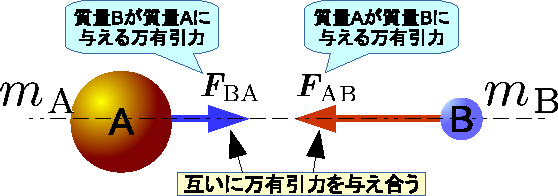
\includegraphics[keepaspectratio, width=7.2cm,height=6.64cm,clip]{bannyuuinnryoku.pdf}
                    \caption{万有引力}
                    \label{fig:bannyuuinnryoku}
                \end{center}
            \end{figure}

            以上のことを,もう一度もう少しかしこまった言い方で確認しておこう.
            2つの重力質量 $m_{\rm{gA}}$,$m_{\rm{gB}}$ が存在すると,その重力質量
            同士が互いに引き合う.
            これが \textbf{万有引力の法則} である.
            以下の式は 重力質量 $m_{\rm{gA}}$が,重力質量 $m_{\rm{gB}}$ に引っ張られる力を表す.
            力と重力質量 の添え字に注意すること.
                \begin{myshadebox}{万有引力の法則}
                    万有引力(重力質量 $m_{\rm{gA}}$が,重力質量 $m_{\rm{gB}}$ に引っ張られる力)
                    は次式で定義される.
                    \begin{align}\label{Grav}
                        \bF_{\rm{AB}}
                        = -G\frac{m_{\rm{gA}}m_{\rm{gB}}}{{\left| \br_{A}
                        -\br_{B} \right|}^{2}}
                        \frac{\br_{A}-\br_{B}}{\left| \br_{A}
                        -\br_{B} \right|}.
                    \end{align}
                    ここに,$\br_{A}$,$\br_{B}$は,それぞれ$m_{\rm{gA}}$と$m_{\rm{gB}}$の 位置である.
                \end{myshadebox}

                \begin{figure}[hbt]
                    \begin{center}
                        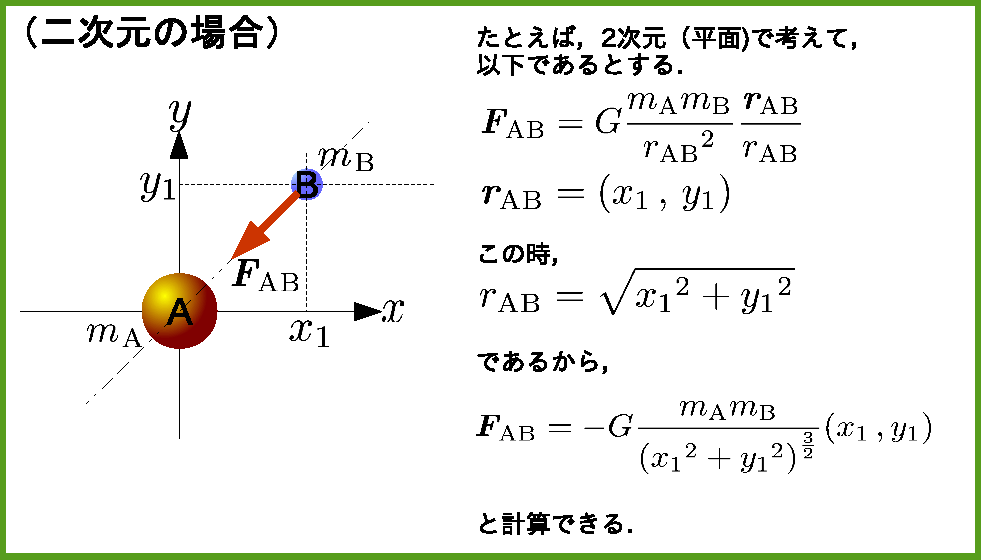
\includegraphics[keepaspectratio, width=6.5cm,height=4.2cm,clip]{bannyuuinnryoku_rei2d.pdf}
                        \caption{万有引力(例:2次元)}
                        \label{fig:bannyuuinnryoku_rei2d}
                    \end{center}
                \end{figure}

            \begin{memo}{万有引力法則とケプラーの法則}
                ニュートンが万有引力の法則を見つけたのは,
                \textbf{ケプラーの惑星の運動の3法則} を
                説明するためであった.たしかに,
                万有引力をニュートンの運動の3法則を
                用いると,ケプラーの法則が満たされる.
                逆に,ケプラーの法則から万有引力を
                導ける.どちらを基本法則としてもよいと
                思われるが,ここは万有引力を
                基本法則としたほうが無難だろう---
                ケプラーの法則は3つであり,
                万有引力は1つであるから…これも思考経済だ---
            \end{memo}

            \subsection{重力質量}
            万有引力の法則で表される質量のことを,\textbf{重力質量} という.
            重力質量は,運動方程式で表される慣性質量とは,別の概念である.
            重力質量は物体の「重さ」を表現していると考えられる
                \footnote{
                    慣性質量とは,物体の動きにくさ を表すものであった.
                }.
            また,重力質量$m_{\rm{gB}}$が 重力質量$m_{\rm{gA}}$に引っ張られる力 $\bF_{\rm{BA}}$ は
                \begin{align}
                    \bF_{\rm{BA}}
                    =-G\frac{m_{\rm{gB}}m_{\rm{gA}}}{{\left| \br_{B}
                    -\br_{A} \right|}^{2}}
                    \frac{\br_{B}-\br_{A}}{\left| \br_{B}
                    -\br_{A} \right|}
                \end{align}
            である.
            $\bF_{\rm{AB}}$ と $\bF_{\rm{BA}}$ の関係は,明らかに
            ($\br_{B}-\br_{A}$の部分に注目)
                \begin{align}
                    \bF_{\rm{AB}}=-\bF_{\rm{BA}}
                \end{align}
            であることがわかり,作用反作用の法則が成立していることも確認できる.

            \begin{memo}{この世界にある「力」の種類}
            万有引力は基本的な力の1つである.基本的な力はこの他に3つあって,
            それは「電磁気的な力」,「弱い力」,
            「核力」である.力のことを \textbf{相互作用} ということもある.

             古典力学でいう力とは, 主に,電磁気的な力 と 万有引力 である.
            \end{memo}

            \subsection{重力加速度}
                万有引力の法則は,2つの物体間に関する法則である.
                ここで,違う視点から,万有引力の法則を眺めてみる.
                物体の一つを惑星,もう一方を任意の物体と考えてもらいたい.
                物体が惑星に引っ張られているイメージ.

                惑星の質量を,$M_{P}$,惑星の位置を $\br_{P}$ とする.
                    \footnote{
                        添字の $P$ は Planet の頭文字.
                    }.
                また,惑星上の物体の質量を $m_{\mathrm{g}}$,位置を $\br$ とする.

                すると,物体が惑星から受ける力は,以下の式で表せる.
                    \begin{equation*}
                        \bF
                        =-m_{\mathrm{g}}\left( G\frac{M_{P}}{{\left| \br-\br_{P} \right|}^{2}}
                        \frac{\br-\br_{P}}
                        {\left| \br-\br_{P}\right|}\right).
                    \end{equation*}
                ここに,$\br$,$\br_{P}$ はそれぞれ,質点の位置 と 惑星の位置 を表す.

                今基準としているのは惑星だから,惑星の位置を基準にすれば($\br_{P}=\bzero$),
                    \begin{equation*}
                        \bF
                        =-m_{\mathrm{g}}\left( G\frac{M_{P}}{{\left| \br \right|}^{2}}
                        \frac{\br}
                        {\left| \br\right|}\right).
                    \end{equation*}

                ここで,\textbf{重力加速度} を以下で定義する.
                        \begin{myshadebox}{重力加速度の定義}
                            次式で,重力加速度を定義する.
                            \begin{align}\label{eq:GravAccer000}
                                \textit{\textbf{g}} :=
                                G\frac{M_{P}}{{\left| \br \right|}^{2}}
                                \frac{\br}{\left| \br \right|}.
                            \end{align}
                        \end{myshadebox}

                万有引力の法則に,惑星の質量 $M_{P}$,惑星の位置 $\br_{P}=\bzero$ を代入している.
                この定義において,重力加速度の向きは惑星から質点に向かう方向である.従って,鉛直上向きを正とする.
                この重力加速度は惑星の近くではほぼ一定であるとみなせる.従って,惑星の表面付近から受ける力は,重
                力加速度を用いて,
                    \begin{align}
                        \bF =- m_{\mathrm{g}}\textit{\textbf{g}}
                    \end{align}
                と書ける.すなわち,質点は地表よりも上に存在するとき
                    \footnote{
                        地表:地球の表面のことをいう.
                    },
                質点は惑星に向かう方向に重力を受けることになる.負の符号が付いている理由は,
                惑星から質点に向かう方向を正方向にとっているため.



\chapter{保存則}
%   %-----------------------------------------------------------------------------------------------
%   %  Input
%   %    File Name : PhysNote_CM_ConservationLaw.tex
%   %    説明      : ニュートンの運動の法則から導かれる,各種保存則を記述する.
%   %-----------------------------------------------------------------------------------------------
        %   %==========================================================================
%   %  Section
%   %==========================================================================
    \section{等価原理}
%       %======================================================================
%       %  SubSection
%       %======================================================================
        \subsection{原理}
        運動方程式で定義される 慣性質量 と,万有引力から定義される 重力質量 は全く別の概念である.慣
        性質量は「物体の動きにくさ」を表していて,重力質量は「物体の重さ」を表現しているのであって,
        両者が等しい必要性は全くない.しかし,経験的に,慣性質量と重力質量は等価であることが知られて
        いる.「重い物体ほど動かしにくくなる」ということは,誰しもが経験していることと思う.そして,
        E\"{o}tv\"{o}sという人が実験で確認している.そこで,\textbf{慣性質量と重力質量は等価である} と
        いうことを認めて,これを式で書くと次のようになる.
                \begin{myshadebox}{等価原理}
                    等価原理を表す式は,次の通り.
                    \begin{align}
                        m_{\mathrm{i}} := m_{\mathrm{g}}.
                    \end{align}
                \end{myshadebox}

        この式が \textbf{等価原理} の根本を表す式である.
        この原理に従って,以下では,重力質量や慣性質量の区別なしに,単に「質量」ということにする.

%       %======================================================================
%       %  SubSection
%       %======================================================================
        \subsection{実験による確認}
            エトヴェシュ
                \footnote{
                    V\'{a}s\'{a}rosnam\`{e}nyi B\'{a}r\'{o} E\"{o}tv\"{o}s Lor\'{a}nd(1848 -- 1919,ハンガリー):
                    ここに記載している通り,重力質量と慣性質量が等価であることを,実験的に確かめた.
                }
            の行った実験は,多くの物質の,慣性質量の重力質量の比を測定し,その比が等しいこ
            とを確かめる実験を行い,その結果,どの物質でも慣性質量と重力質量の比はある一定の値に一致する
            ことが示された.多くの物質でその比が一定値をとるということは,慣性質量と重量質量は等価である
            と考えられる.しかし,絶対に等価であるとは言い切れない.つまり,この等価原理は実験的に正しい
            と推測されているだけで,“本当に”両者が等価であることが説明されたわけではない.もしかしたら,
            わずかな違いがあるのかもしれない.

            この原理を受け入れる1つの理由として,この等価原理を仮定しその上で理論を組み立て,多くの物理
            現象を説明できるなら,この等価原理は正しいと認識してよいだろうと考える.実際,アインシュタインはこの
            等価原理の考えをさらに発展させ,相対性理論を作り上げた.相対性理論は,ニュートン力学をその理論の
            内部に包括し,さらにより一般的に物理現象を説明できている.等価原理を認めることで,多くの物理
            現象を説明できていることから,等価原理は採用すべきもだと言える.本当に正しいかどうかは別
            にして,とりあえず,この原理を仮定して理論を組み立てていくことにしよう.
            \begin{figure}[hbt]
                \begin{center}
                    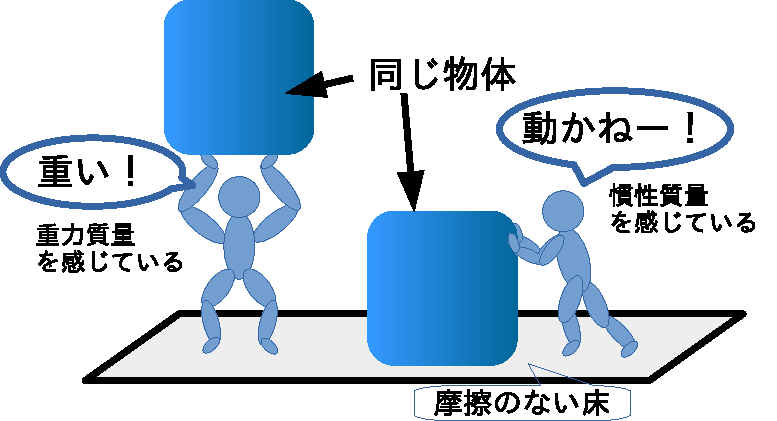
\includegraphics[keepaspectratio, width=6.6cm,height=3.6cm,clip]{toukagennri.pdf}
                    \caption{等価原理}
                    \label{fig:toukagennri}
                \end{center}
            \end{figure}

%   %==========================================================================
%   %  Section
%   %==========================================================================
    \section{運動量保存の法則}
%       %======================================================================
%       %  SubSection
%       %======================================================================
        \subsection{運動量の定義}
            物体の質量 $m$ と質点の速度 $\bv$ の
            積を \textbf{運動量} $\textit{\textbf{p}}$ と定義する.
                \begin{align}
                    \textit{\textbf{p}} := m \bv.
                \end{align}
            このように定義された運動量は,物体の運動の「力強さ」を表現している.
            質量が大きいほど,また,速度が大きいほど運動量が大きくなる.
            また,同じような言い方ではあるが,運動量は他の物体にぶつかったとき,
            与えるダメージの程度を表すのものともいえる.

%       %======================================================================
%       %  SubSection
%       %======================================================================
        \subsection{運動量を用いた運動方程式}\label{運動量_運動方程式}
                ニュートンの運動方程式は式(\ref{eq:N_eq})で示したように,
                    \begin{align}
                        m\frac{\df^{2}\br}{\df t^{2}} = \bF
                    \end{align}
                である.この式は速度 $\bv=\df\br/\df t$ を用いて表すと,
                    \begin{align}\label{eq:N_peq}
                        m\frac{\df\bv}{\df t} = \bF
                    \end{align}
                である.

                さて,今まで考えてきたニュートンの運動方程式は,暗黙のうちに
                “質点の慣性質量は時間変化しない”という
                約束されている式である.従って,慣性質量が時間変化するときには,
                上式のような運動方程式では現象
                を正確に記述できない.どうすればよいかといえば,当たり前のことだが,
                質点の慣性質量の時間変化を考
                慮に入れた式に書き直せばよい.そのような式を作ることは簡単で,
                慣性質量 $m_{\mathrm{i}}$ を時間変
                化するとして,つまり $m_{\mathrm{i}}=m_{\mathrm{i}} (t)$ と考えて,
                微分記号の中に入れてしま
                えばよい.慣性質量 $m_{\mathrm{i}}$ を微分記号の中に入れると,
                    \begin{align}
                        \frac{\df \left( m\bv\right)}{\df t} = \bF
                    \end{align}
                となる.ここで運動量 $\textit{\textbf{p}} := m \bv$ を用いると,次を得る.
                        \begin{myshadebox}{運動量表示の運動方程式}
                            運動量 $\bp$ を用いた運動方程式は,次のように表現できる.
                            \begin{align}\label{6}
                                \frac{\df\textit{\textbf{p}}}{\df t} = \bF.
                            \end{align}
                        \end{myshadebox}

                これが,運動量を用いた運動方程式である.この表記もよく用いられる.
                この式は,慣性質量が時間変化しない場合と時間変化する場合の両方で,
                成立する式である.念のために,それを示しておく.運動量の時間微分は,
                積の微分公式
                    \footnote{
                        積の微分公式とは,以下のようなものであった.
                        \begin{equation*}
                            \frac{\df }{\df t}\left( f(x)g(x) \right)
                            =
                            g(x)\frac{\df f(x)}{\df x}+f(x)\frac{\df g(x)}{\df x}
                        \end{equation*}
                    }
                を用いると以下のようになる.
                    \begin{align}
                        \frac{\df\textit{\textbf{p}}}{\df t}
                        =\frac{\df \left(m\bv\right)}{\df t}
                        =m\frac{\df\bv}{\df t}
                        +\bv\frac{\df m}{\df t}
                    \end{align}
                慣性質量が時間変化していると考えていることに注意すること.これを用いると運動方程式は
                    \begin{align}
                        m\frac{\df\bv}{\df t}
                        +\bv\frac{\df m}{\df t}
                        =\bF
                    \end{align}
                と書ける.慣性質量が時間変化していなければ,左辺2項は0になって,式(\ref{eq:N_peq})
                に帰着する.

                \begin{memo}{運動量を用いた運動方程式の必要性}
                    この運動量を用いた運動方程式の表記は,特に相対性理論を学習するときに
                    必要となる.とはいっても,もっと身近な所にも,この運動量を用いた運動方程式を
                    考えることは多い.例えば,車はガソリンを燃料にして動くが,このガソリンは時間と共に
                    なくなっていく.つまり,車の質量が,時間変化しているのである---実際はこの質量の変化は,
                    車本体の質量に対して,無視できる程度だが.

                    また,宇宙へロケットを打ち上げる場合も,燃料の燃焼による質量の変化を考える必要がある.
                    物体の運動中に,その質量が時間変化するので,運動量でかかれた運動方程式が必要になる.

                    質量を定数扱いできない場合には,運動量表記による運動方程式を使わないといけない.
                \end{memo}
                    \begin{figure}[hbt]
                        \begin{center}
                            \includegraphicsdefault{undoryo_rocket.pdf}
                            \caption{運動量を用いた方程式の適用例}
                            \label{fig:rocket1}
                        \end{center}
                    \end{figure}


%       %======================================================================
%       %  SubSection
%       %======================================================================
        \subsection{運動量保存の法則}
%       %======================================================================
%       %  SubsubSection
%       %======================================================================
        \subsubsection{2つの物体間の運動量保存の法則}
            2つの物体が衝突したとき,
            衝突\textbf{前}の2つの物体の運動量の和 と 衝突\textbf{後}の2つの物体の運動量の和 は同じ値をとる.
            つまり,2つの物体の運動量の和は,衝突が起ころうとも, \textbf{時間によらずに一定値をとる}のである.
            この法則を,\textbf{運動量保存の法則} という.
            または略して,\textbf{運動量保存則} ともいう.この法則を式で表すことを考える.
            衝突前の2つの物体の運動量をそれぞれ,$\textit{\textbf{p}}_{1\mbox{前}}$ ,
            $\textit{\textbf{p}}_{2\mbox{前}}$ とする.
            これらにより,衝突前の運動量の和
            は $\textit{\textbf{p}}_{1\mbox{前}}+\textit{\textbf{p}}_{2\mbox{前}}$ である.
            衝突後の2つの物体の運動量をそれぞれ,
            $\textit{\textbf{p}}_{1\mbox{\mbox{後}}}$ ,$\textit{\textbf{p}}_{2\mbox{後}}$
            とする.これらにより,衝突後の運動量の和
            は $\textit{\textbf{p}}_{1\mbox{後}}+\textit{\textbf{p}}_{2\mbox{後}}$ である.
            運動量保存の法則によると,“衝突前の運動量の和”と“衝突後の運動量の和”
            は同じ値をとるので,
                \begin{align}
                    \textit{\textbf{p}}_{1\mbox{前}}+\textit{\textbf{p}}_{2\mbox{前}}
                    =\textit{\textbf{p}}_{1\mbox{後}}+\textit{\textbf{p}}_{2\mbox{後}}
                \end{align}
            の関係があることになる.

%       %======================================================================
%       %  SubsubSection
%       %======================================================================
        \subsubsection{$N$ 個の物体間の運動量保存の法則}
            物体が $N$ 個だけ存在する場合に拡張しても,この法則は成り立つ.これを式で書くと,
                                \begin{align}
                    \sum_{i=1}^{N}\textit{\textbf{p}}_{i\mbox{前}} = \sum_{i=1}^{N}\textit{\textbf{p}}_{i\mbox{後}}.
                                \end{align}
                        となる
                                \footnote{
                                        和の記号を展開すると,以下のようになる.
                        \begin{align*}
                            \sum_{i=1}^{N}\textit{\textbf{p}}_{i\mbox{前}} &=  \textit{\textbf{p}}_{1\mbox{前}}+\textit{\textbf{p}}_{2\mbox{前}}+\cdots+\textit{\textbf{p}}_{N\mbox{前}}. \\
                            \sum_{i=1}^{N}\textit{\textbf{p}}_{i\mbox{後}} &=  \textit{\textbf{p}}_{1\mbox{後}}+\textit{\textbf{p}}_{2\mbox{後}}+\cdots+\textit{\textbf{p}}_{N\mbox{後}}.
                        \end{align*}
                }.

            但し,これは $N$ 個の物体が同時に衝突する場合 についての式である.
            これが運動量保存の法則を表現する式である.この式をさらに見やすい形にしよう.
            衝突前と衝突後で 各物体の運動量の総和 が同じ値をとるので,
                \begin{align}
                    \textit{\textbf{P}} := \sum_{i=1}^{N}\textit{\textbf{p}}_{i\mbox{前}}
                    = \sum_{i=1}^{N}\textit{\textbf{p}}_{i\mbox{後}}
                \end{align}
            とおける.衝突時には1つ1つの物体は力を受けるわけだが,
            全ての物体が受ける力を合計すると 0 になる.
            このことは,作用反作用の法則を思い出せば納得できる.1つの物体が,
            別のもう1つ物体に力を与えるとき,
            作用反作用の法則により,与えた力と逆向きで大きさの等しい力を受けるからである.
            作用反作用によって生じる力の合計は0になることは前に確認した.
            従って,運動量を用いた運動方程式(\ref{6})を
            おもい起こせば,次を得る.
                    \begin{myshadebox}{運動量保存の法則}
                        運動量保存の法則は,次式で表せる.
                        \begin{align}\label{61}
                            \frac{\df\textit{\textbf{P}}}{\df t} = 0.
                        \end{align}
                    \end{myshadebox}

            $\textit{\textbf{P}}$ が時間によらずに一定値をとることからも,
            この式は正しいと言える.従って,この式(\ref{61})も
            運動量保存の法則を表現しているのである.
                \begin{figure}[hbt]
                    \begin{center}
                        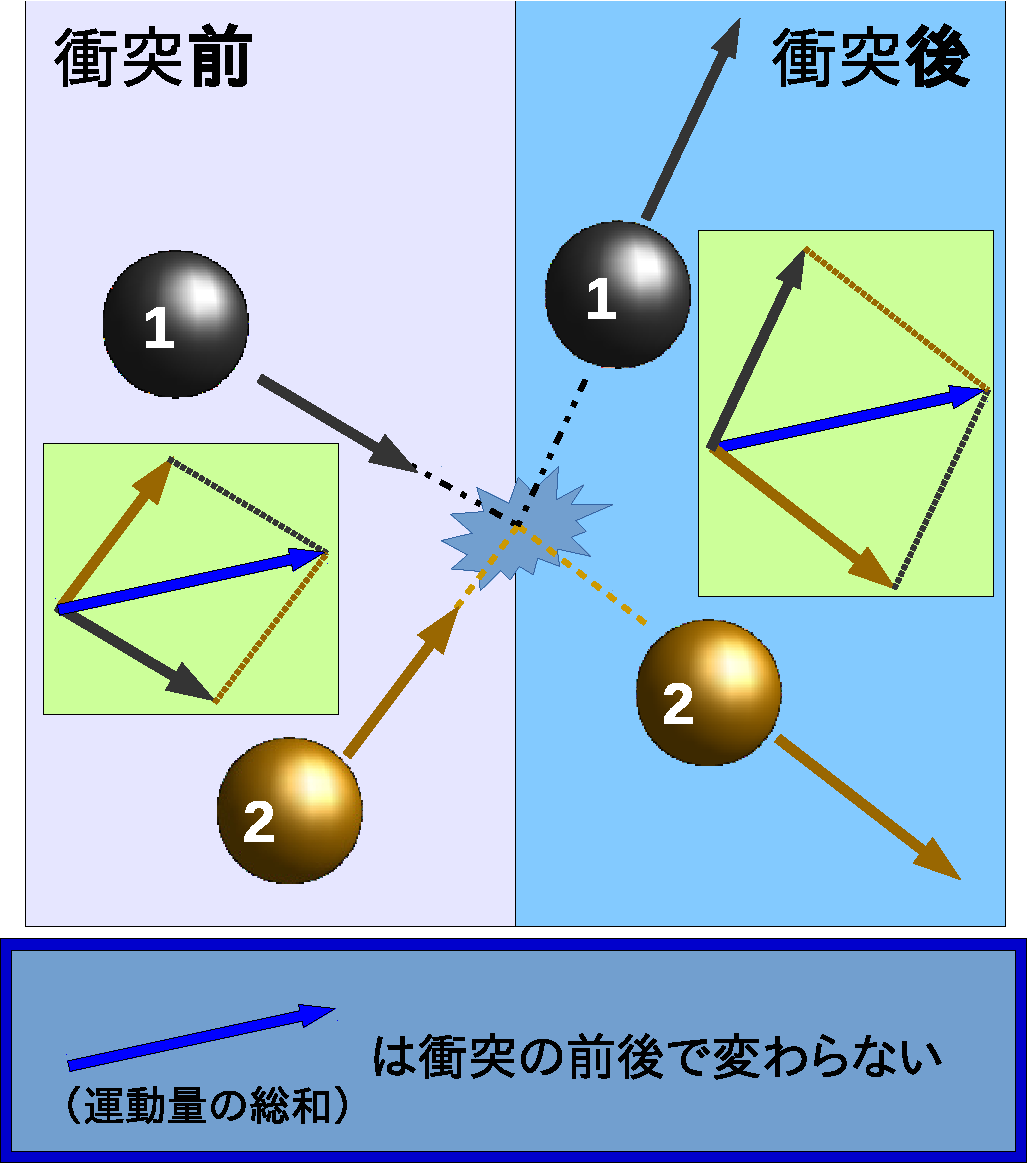
\includegraphics[keepaspectratio, width=6cm,height=8cm,clip]{P_hozonnsoku2.pdf}
                        \caption{運動量保存の法則}
                        \label{fig:Hozonasu}
                    \end{center}
                \end{figure}

            \begin{memo}{現象全体を見ることで,保存則が成立する}
                運動量保存の法則は,系の全ての物体について見渡すことで,成立している法則である.
                例えば,衝突に関係する物体全体の中の,一部の物体だけを見ているならば,
                この法則は成り立たない.1つの物体が運動量を増加させれば,
                別の物体は運動量を減少させるのである.
                この法則が意味していることは,この増加量と減少量の和が0になる ということである.
            \end{memo}

            \begin{memo}{運動方程式と運動量保存則}
                運動量保存の法則を次のように考えることもできる.すなわち,
                運動方程式$\df\textit{\textbf{P}}/\df t = \bF$ で,
                $\bF=0$ のとき,$\df\textit{\textbf{P}}/\df t =0$ である.
                従って,運動量保存の法則は運動方程式から導かれる.
            \end{memo}

            \begin{memo}{高校物理における運動量保存則}
                高校の物理学では,2つの物体の衝突を考えて,運動量保存の法則を説明した.
                より具体的な式で表現すれば,
                \begin{align}
                m_{a}\bv_{a\mbox{前}}+m_{b}\bv_{b\mbox{前}}=m_{a}\bv_{a\mbox{後}}+m_{b}\bv_{b\mbox{後}}
                \end{align}
                である.
            \end{memo}


%       %======================================================================
%       %  SubSection
%       %======================================================================
        \subsection{運動量の変化と力積}
            ある1つの物体の運動量が時間変化した場合について考える.物体が壁に当たって,
            運動方向を変化させる現象を想像するとよい.
            変化前と変化後の運動量をれぞれ,$\textit{\textbf{p}}_{\mbox{前}}$,
            $\textit{\textbf{p}}_{\mbox{後}}$ と書く.
            そして,このときの運動量の変化を $\textit{\textbf{I}}$ と書くことにすると,
                \begin{align}\label{7}
                    \textit{\textbf{I}} = \textit{\textbf{p}}_{\mbox{後}}-\textit{\textbf{p}}_{\mbox{前}}
                \end{align}
            である.

            ところで,物体が運動の方向を変化させたのだから,物体は力を受けたはずである.
            なぜなら,慣性の法則によると,
            物体に力が働かない限り,物体は等速直線運動をするからである.
            しかし,物体の運動量が変化したということは
            運動量の定義 $\textit{\textbf{p}} := m_{\mathrm{i}} \bv$ から,
            速度が変化したことになる.
            すなわち,加速度を生じたわけであり,力が加わったと解釈できる
                \footnote{
                    「加速度が生じること」と「力が加わること」は,運動方程式から,
                    同じことを意味すると言える.
                }.
            その力を $\bF$ とすると,運動方程式(\ref{6})から,
                \begin{align}
                    \frac{\df\textit{\textbf{p}}}{\df t} = \bF
                \end{align}
            をたてられる.この式の両辺を,衝突前の時間 $t_{\mbox{前}}$ から
            衝突後の時間 $t_{\mbox{後}}$ で定積分すると,
                \begin{align}\label{8}
                    \int_{t_{\mbox{前}}}^{t_{\mbox{後}}}\frac{\df\textit{\textbf{p}}}{\df t} \df t
                    &= \int_{t_{\mbox{前}}}^{t_{\mbox{後}}}\bF \df t \notag \\
                    \Leftrightarrow \int_{t_{\mbox{前}}}^{t_{\mbox{後}}}\df\textit{\textbf{p}}
                    &= \int_{t_{\mbox{前}}}^{t_{\mbox{後}}}\bF \df t \notag \\
                    \Leftrightarrow \textit{\textbf{p}}(t_{\mbox{前}})-\textit{\textbf{p}}(t_{\mbox{後}})
                    &= \int_{t_{\mbox{後}}}^{t_{\mbox{前}}}\bF \df t
                \end{align}
            となる.この式の左辺は,$\textit{\textbf{p}}_{\mbox{後}}-\textit{\textbf{p}}_{\mbox{前}}$ と
            全く同じことであるので,
            式(\ref{7})と式(\ref{8})を見比べると,
                \begin{align}
                    \textit{\textbf{I}} = \int_{t_{\mbox{前}}}^{t_{\mbox{後}}}\bF \df t
                \end{align}
            の関係を得る.この $\textit{\textbf{I}}$ のことを,\textbf{力積} という.
            つまり,運動量変化は力積 $\textit{\textbf{I}} =\int_{t_{\mbox{前}}}^{t_{\mbox{後}}}\bF \df t$
            によって生じたと考えられる.


%   %==========================================================================
%   %  Section
%   %==========================================================================
    \section{角運動量保存の法則}
        \begin{mycomment}
            回転している物体に共通する性質はあるだろうか.回転する物体として
            よく例に上がるのがコマである.また,車輪の例もよく見かける.
            回転するコマが倒れずに回転を続けられる理由や,走行中の自転車が
            安定している理由に,これから説明する角運動量保存の法則が絡んでいる.
        \end{mycomment}

%       %======================================================================
%       %  SubSection
%       %======================================================================
        \subsection{角運動}
            物体が一直線上を運動していても,ある固定された点からその物体の運動を眺めると,
            その点を中心として回転しているように見える.
            例えば,車が走っているのを見るとき,その車を1つの決まった場所から目で追うためには,
            首(あるいは目)を回転させる必要がある.
            このような回転運動のことを \textbf{角運動} という.
            (回転を表すのに角度を用いるからだろうか?)このような状況を思い浮かべつつ,
            角運動について考える.
            角運運動量を記述するには,ベクトルの \textbf{外積} の知識が必要である.

        \subsection{てこの原理}
            物体の回転の最も基本的な原理は,\textbf{てこの原理} である.
            そのままでは簡単には持ち上げられない程,重い物体があるとしよう.
            この物体を持ち上げたいとき,てこの原理が役に立つ.
            もはや,説明するまでもないだろう.図\ref{fig:teko_no_genri1}を見れば,
            分かるはずである.直接的に力を加えている部分を \textbf{力点},
            棒の回転の支えになっている点を \textbf{支点},重い物体に力がかかっている
            点を \textbf{作用点} という.
                    \begin{figure}[hbt]
                        \begin{center}
                            \includegraphicssqmid{teko_no_genri1.pdf}
                            \caption{てこの原理}
                            \label{fig:teko_no_genri1}
                        \end{center}
                    \end{figure}

            てこの原理は,重い物体を小さな力で持ち上げることを,可能にする.
            てこの原理を数式で表現してみよう.力点にかかる力を $F$ とし,
            持ち上げたい物体にかかる力(重力)を $W$ とする.
            てこの原理を使わずに,物体を持ち上げようとしても,
            加える力よりも物体の方が重く,すなわち
                \begin{equation*}
                    F < W
                \end{equation*}
            となるので,物体を持ち上げられない.

            てこの原理を使うと,上式が成り立っていても,物体を持ち上げることができる.
            支点と力点との距離を $l_{1}$,支点と作用点との距離を $l_{2}$ としよう.
            このとき,物体が持ち上がったとすると,てこの原理は
                \begin{align}
                    Fl_{1} > Wl_{2}
                \end{align}
            のように表現される.この式が成立するときに,物体を持ち上げられるの
            物体の重さ $W$ は一定であり,力 $F$ には限界値があることから,
            自由に動かせるのは ${l}_{1}$, ${l}_{2}$ しかない.
            支点から力点までの距離(${l}_{1}$)を長くし,
            支点から作用点までの距離(${l}_{2}$)を短くすることで,
            より小さい力で物体を持ち上げることが可能になる.

        \subsection{釣り合いの式}
            てこの原理の式の不等号を等号に置き換えた式を,釣り合いの式という.
                \begin{align}
                    {F}_{1}{l}_{1} = {F}_{2}{l}_{2}.
                \end{align}
            ${F}_{1}$ を物体の重さによってかかる力とし(力点),${F}_{2}$ を棒が傾かないように支える力とする(作用点).
            ${l}_{1}$ は支点と力点との距離で,${l}_{2}$ は支点と作用点との距離である.
                    \begin{figure}[hbt]
                        \begin{center}
                            \includegraphicslarge{TekonoGenri111.pdf}
                            \caption{釣り合い}
                            \label{fig:TekonoGenri111}
                        \end{center}
                    \end{figure}

%       %======================================================================
%       %  SubSection
%       %======================================================================
        \subsection{物体の回転の表現 と ベクトルの外積}
            物体が回転しているということを表現するのに,
            ベクトルの \textbf{外積} という概念を導入する.
            ここでは,このベクトルの外積について考える.

            物体が回転するということは,その軌道は円であるから,
            回転には必ずこの軌道円の中心を通る“回転の軸”が存在する.この回転の軸は直線であることは
            当たり前であって,確認するまでもない.この軸を用いて,回転の方向を表現するのである.
            回転の方向をこの軸方向にとって,回転の強さを適当に定義すれば,
            その回転の特徴を表現できる.さて,以下では回転の具体的な表現の仕方について
            考えていくことにしたいと思う.

            まず,回転の方向の決定方法である.これには回転の軸を用いることは先ほど書いたところである.
            その
            方向には正方向と負方向の2つがあるが,
            その取り決めは次の約束に従うものとされる.すなわち,回転の向きを
            \textbf{「
            速度の方向 $\bv$ の方向から,
            物体から軸へ垂線を下ろした向き($\textbf{\textit{k}}$ の方向)に
            右ねじを回して進向き」} と決めるのである.
            これを \textbf{右ねじの法則} という.
            回転の強さについてはもう少し後で考えるこにする.
                        \begin{figure}[hbt]
                            \begin{center}
                                \includegraphicssqmid{gaiseki1new.pdf}
                                \caption{物体の回転}
                                \label{fig:gaiseki1new}
                            \end{center}
                        \end{figure}

            右ねじの法則によって方向を定義されたベクトルを $\bL$ と書くことにする.
            これを,
            \begin{align}
            \bL=\textbf{\textit{k}} \times \bv
            \end{align}
            のように表現する.この式の解釈の仕方は,
            「ベクトル $\textbf{\textit{k}}$ をベクトル $\bv$ 方向へ右ねじ回して進む
            向き」のベクトルと読む.

            しかし,向きを設定したのではまだ不十分である.この $\bL$ の大きさを考える必要がある.
            そこで,大きさの定義として,「物体の速度ベクトル $\bv$ と
            垂線ベクトル $\textbf{\textit{k}}$ のなす平行四辺形の面積」を
            用いる.このような,ベクトルの大きさの定義の理由については後回しにして,
            ここではそのようなものであると考えておいてもらいたい.式でこの定義を表現すれば,
            \begin{align}
                L:=\|\bL\|=\|\textbf{\textit{k}} \times \bv\|
                =\| \textbf{\textit{k}} \| \| \bv \| \sin\theta
            \end{align}
            である.

            さて,ベクトルの大きさの具体的な
            定義を見てもらったところで,
            次にこの定義の意味の説明である.

            覚え方は,内積を定義したときには $\cos$ 関数を
            用いて定義したことと比べると,今回は
            この部分は $\sin$ 関数となっていることに注意すればよい
            ということだろうか.

            大体,物体の回転をベクトルを用いて表現すると
            以上のような感じだが,しかしこれでは感覚的過ぎる.
            そこで,この物体の回転を,ベクトルの成分を通して
            もう少し詳しく考えていくことにしたい.

%       %======================================================================
%       %  SubSection
%       %======================================================================
        \subsection{角運動量}
                \begin{figure}[hbt]
                    \begin{center}
                        \includegraphicssqmid{kaku_unndouryou2.pdf}
                        \label{fig:kaku_unndouryou2}
                        \caption{(a) 直線運動}
                    \end{center}
                \end{figure}
                \begin{figure}[hbt]
                    \begin{center}
                        \includegraphicssqmid{kaku_unndouryou1.pdf}
                        \label{fig:kaku_unndouryou1}
                        \caption{(b) 回転運動}
                    \end{center}
                \end{figure}

                物体が位置 $\br$ において,運動量 $\textit{\textbf{p}}$ をもっているとき,
                            \begin{align}
                            \bL
                            := \br \times \textit{\textbf{p}}
                            \end{align}
                で定義される $\bL$ を原点の周りの \textbf{角運動量} という.
                物体の角運動量 $\bL$ が0でない値をとるとき,その物体は回転運動
                をしていると言える.

%       %======================================================================
%       %  SubSection
%       %======================================================================
        \subsection{角運動の方程式}
                回転運動している物体の運動方程式を考えてみよう.

                角運動量 $\bL$ を時間微分すると,
                    \begin{align}\label{9}
                        \frac{\df\bL}{\df t}
                        = \frac{\df\br}{\df t} \times \textit{\textbf{p}}
                        +\br \times \frac{\df\textit{\textbf{p}}}{\df t}
                    \end{align}
                となる.ここで,式(\ref{9})の第1項の運動量 $\textit{\textbf{p}}$ は
                    \begin{align}
                        \textit{\textbf{p}} = m\bv=m\frac{\df\br}{\df t}
                    \end{align}
                である.これを用いて,
                    \begin{align}\label{9_1}
                        \frac{\df\bL}{\df t}
                        = \frac{\df\br}{\df t} \times m\frac{\df\br}{\df t}
                        +\br \times \frac{\df\textit{\textbf{p}}}{\df t}
                    \end{align}
                となるが,ベクトルの外積の性質
                (任意のベクトル $\bA$ に対して $\bA \times \bA=0$ が成り立つ)
                を考慮すると,
                    \begin{align}
                        \frac{\df\br}{\df t} \times m\frac{\df\br}{\df t}
                        =m\left( \frac{\df\br}{\df t} \times \frac{\df\br}{\df t} \right)=0
                    \end{align}
                となってしまうので,式(\ref{9_1})の第1項は 0 にってしまい,結局,
                    \begin{align}
                        \frac{\df\bL}{\df t} = \br \times \frac{\df\textit{\textbf{p}}}{\df t}
                    \end{align}
                と計算される.さらに,運動量を用いた運動方程式(\ref{6})の関係から,
                    \begin{align}\label{10}
                        \frac{\df\bL}{\df t} = \br \times \bF
                    \end{align}
                を得る.ここで,原点の周りの \textbf{力のモーメント} $\bN$を
                    \begin{align}\label{12}
                        \bN := \br \times \bF
                    \end{align}
                と定義すると,式(\ref{10})は
                    \begin{align}\label{11}
                        \bN = \frac{\df\bL}{\df t}
                    \end{align}
                と書ける.式(\ref{11})は,運動量を用いた運動方程式(\ref{6})と同じ形の式になっている.
                ($\bN$ → $\bF$,
                $\bL$ → $\textit{\textbf{p}}$ とするとわかる.)
                従って,式(\ref{11})は角運動についての運動方程式であると言える.
                力のモーメント $\bN$ は,角運動を引き起こす力である.
                すなわち,$\bN$ は回転運動を引き起こす力であると言える.
                このように回転力を起こす $\bN$ は \textbf{トルク} ともよばれる.

%       %======================================================================
%       %  SubSection
%       %=====================================================================
        \subsection{角運動量保存則}
                運動量保存則を考えたときに,
                「外部から力 $\bF$ が加わらない限り,全物体の運動量の総和は一定である」
                ということを確認した.
                角運動量についても同様な法則が成り立っていて,これを \textbf{角運動量保存の法則} という.
                または略して,\textbf{角運動量保存則} という.
                では,角運動量保存則 を式で表すことを考える.外力が働かないことから,$\bF=0$ であって,
                これを力のモーメントの定義式(\ref{12})に代入することで,
                $\bN := \br \times 0 =0$ を得る.よって,
                この $\bN=0$ を角運動についての運動方程式(\ref{11})に代入して,
                \begin{equation*}
                    \frac{\df\bL}{\df t} = 0
                \end{equation*}
                となる.この式は,外力が働かなければ,角運動量の時間変化がないことを示している.
                つまり,時間によらずに一定値をとることを意味する.従って,式(\ref{13})
                は角運動量保存則を表現した式であると言える.
                    \begin{myshadebox}{角運動量保存則}
                            位置ベクトル $\br$ にある物体に外力が働いていない場合($\bF=0$),
                            角運動量 $\bL$ は時間経過にかかわらず,一定に保たれる.
                            \begin{align}\label{13}
                                \frac{\df\bL}{\df t} = 0
                            \end{align}
                    \end{myshadebox}

                角運動量保存則を積分すれば,定ベクトルを得る.実際に確かめてみよう.
                角運動量保存則は 式(\ref{13})により $\df\bL/\df t = 0$ である.
                この角運動量 $\bL$ は $\bL
                := \br \times \textit{\textbf{p}}$ で定義される量であった.従って,
                角運動量保存則は
                    \begin{align}
                        \frac{\df \left(\br \times \textit{\textbf{p}}\right)}{\df t} = 0
                    \end{align}
                と表現しても同じことである.そして,両辺を時間で積分して,
                    \begin{align}
                        \int\left(\frac{\df \left(\br \times \textit{\textbf{p}}\right)}{\df t}\right) \df t = \bC
                    \end{align}
                ここに, $\bC$ は定ベクトルである.よって,
                    \begin{align}
                        \br \times \textit{\textbf{p}}=\bC
                    \end{align}
                を得る.この式は,位置 $\br$ が原点から遠くなるほど,運動量は小さくなることを意味している
                逆にいえば,原点に近いほど,運動量は大きくなるのである.

                例えば,スケーターの回転を考えてみる.この場合の座標原点は体の重心にとる.
                スケーターが自身の腕を大きく広げたときほど ゆっくりと回転している のは,手の位置 $\br$ が
                体の重心からより遠くなるためである.すなわち,これは $\br$ が
                大きくなることを意味する.しかし,特に外力が働かないので,(氷との摩擦は無視する)
                角運動量保存の法則 $\br \times \textit{\textbf{p}}=\bC$ が成立している.
                従って,運動量 $\textit{\textbf{p}}$ が小さくなるのである.
                というか,運動量を小さくすることで,角運動量保存則を満たそうとするのである.

                腕を縮めると回転が速くなるのは,この逆で,手の位置 $\br$ が
                体の重心に近づくからである.従って,角運動量保存則を満たすために
                運動量 $\textit{\textbf{p}}$ を大きくするのである.


%   %==========================================================================
%   %  Section
%   %==========================================================================
    \section{力学的エネルギー保存の法則}
%       %======================================================================
%       %  SubSection
%       %======================================================================
        \subsection{仕事}\label{shou_sigoto}
%       %======================================================================
%       %  SubsubSection
%       %======================================================================
        \subsubsection{1次元上の仕事}
                まず簡単に,一方向のみに限定して考える.その一方向を,$x$ 方向とする.
                さて,物体に外力 $F_{x}$ を加えて, $x$ 方向に $\Delta x$ だけ変位させたとしよう.
                物体の移動は,物体に与えた外力 $F_{x}$ とその変位の大きさ $\Delta x$ できまる.
                この移動は,物体が「仕事」をされたから,生じたものであると考える.仕事は,記号 $W$ で
                表され,次式よって定義される.
                    \begin{equation*}
                        W  :=  F_{x} \Delta x.
                    \end{equation*}
                単位は上の定義式から,[Nm] である.仕事の単位を表す記号は [J] が使われる.
                つまり,[J] = [Nm] である.単位については後で改めて,記述しよう.

                「仕事」という概念を導入することで,物体の移動を考えやすくなる.物体が
                移動したということは,物体に外力が働いて,変位したということであるが.
                その力の方向と変位の方向を考慮する必要がない場合,
                    \begin{equation*}
                        \mbox{物体は「仕事」} W \mbox{をされた.}
                    \end{equation*}
                あるいは,視点を変えて,
                    \begin{equation*}
                        \mbox{「仕事」} W \mbox{をした.}
                    \end{equation*}
                と表現できる
                    \footnote{
                        もう少し学習を進めると,「エネルギー」という概念が導入される.この「エネルギー」を
                        説明するために,「仕事」が使われるのであるが,実は後で記述するように,仕事と
                        エネルギーには,表と裏のような関係がある.「エネルギー」は,物理学で最も重要な
                        概念の1つである.
                    }.
                一方向だけで考えられるならば仕事の定義は上の式で十分である.

%       %======================================================================
%       %  SubsubSection
%       %======================================================================
        \subsubsection{3次元内の仕事}
                物体に力を加えたときの物体の変位の方向は,必ずしも,その力の方向であるとは限らない.
                変位も3次元を考えることができて,一方向だけではない.
                例えば,重い荷物を引っ張るとき,真横に力を加えるのではなく,少し上向きに引っ張ることが
                多い.このとき物体は地面から離れず,ただ地面に引きずられるという場合が起こり得る.
                そのとき,力が物体にした仕事は,その力の全てではなく,地面に対して平行な力の成分
                しか仕事をしていない.上向きの成分は,物体が上に上がっていないので,仕事はしていないのである.
                このような場合でも仕事を定義できるように導入されるのが,「なす角」である.
                ここでは,なす角を導入し,$\theta$ で表すことにしよう.
                「なす角」と聞いて,すぐにベクトルの内積が頭に浮かぶと思う.そうベクトルの内積を用いて,
                仕事を定義するのである.

                なす角 $\theta$ を導入すると,力を加えた方向と異なる向きに物体が移動したときにも,
                仕事を定義できるのである.
                    \begin{figure}[hbt]
                        \begin{center}
                            \includegraphicssqmid{sigoto_nasukaku.pdf}
                            \caption{力と仕事(3次元)}
                        \end{center}
                    \end{figure}

                少しかしこまった形で,なす角を導入しよう.
                物体が一定の力 $\bF$ で,\underline{直線距離} $\Delta \textit{\textbf{s}}$ だけ変位したとき,
                \textbf{仕事} $W$を次式で定義する.
                    \begin{align}
                        W:=\bF\cdot\Delta \textit{\textbf{s}}=F\Delta s \cos \theta
                    \end{align}
                ここに,$\theta$ は $F$ と $\Delta s$ の \textbf{なす角} (図\ref{fig:nasu}参照)である.
                    \begin{figure}[hbt]
                        \begin{center}
                            \includegraphicssqmid{nasu.pdf}
                            \caption{力 $\bF$ と変位 $\Delta\textit{\textbf{s}}$ のなす角 $\theta$ }
                            \label{fig:nasu}
                        \end{center}
                    \end{figure}


%       %======================================================================
%       %  SubsubSection
%       %======================================================================
        \subsubsection{仕事の単位}
                仕事の単位は[J]
                    \footnote{
                        ジュールと読む.仕事と熱量の関係を研究した物理学者Jouleの頭文字である.
                    }
                が用いられる.上の仕事の定義からわかるように,仕事の単位はSI単位系
                    \footnote{
                        SI単位系:基本単位として[m](メートル),[Kg](キログラム),[s](セコンド),[A](アンペア)
                        を用いる単位系のこと.\date 現在,SI単位系は国際標準となっている.
                        $\longrightarrow $昔はcgs単位系([cm](センチメートル),[g](グラム),[s])もよく使われていたみたいである.
                        古い教科書を見てみると,cgs単位系で書かれているもの多い.
                    }
                で,
                    \begin{align}\label{eq:Jule}
                        \mathrm{
                            [J]=[Nm]=[kgm^{2}/s^{2}]
                        }
                    \end{align}
                である.

%       %======================================================================
%       %  SubsubSection
%       %======================================================================
        \subsubsection{一般的な仕事の定義}
                次に,物体が 位置によって異なる力 $\bF(\br)$ で,
                \underline{曲線} $\br$ に沿って変位したときの仕事を考える.
                曲線の微小部分 $\df\br$ では力は一定と考えられる.
                よって,この微小部分 $\df\br$ における仕事は
                $\bF(\br) \cdot \df\br$ と書ける.
                すなわち,微小部分での仕事を積分すると,求める仕事 $W$ を得る.従って,位置 $\br_{A}$ か
                ら 位置 $\br_{B}$
                変位が曲線をとるときの仕事は
                    \begin{align}
                        W:=\int_{\br_{A}}^{\br_{B}}
                        \bF(\br) \cdot \df\br
                    \end{align}
                と定義できそうである.しかし,\textbf{これでは不十分である}.なぜなら,位置 $\br_{A}$ から
                位置 $\br_{B}$ までの曲線は無限に作れるからである.というのも
                そのような曲線によって,仕事が異なるからである.これは当たり前のだろう.
                曲線が変わってしまえば,物体の変位する“道のり”が長くなったり,短くなったりするのだから,
                当然,仕事もこの曲線によって異なると考えられる.
                そこで,位置 $\br_{A}$ から
                位置 $\br_{B}$ までの
                この曲線を指定する.それを \textbf{経路} という.位置 $\br_{A}$ から
                位置 $\br_{B}$ までの経路 $C$ に沿って,変位したときの仕事は,次のように書く.
                        \begin{myshadebox}{仕事の定義}
                            経路 $C$ に沿って物体を動かす際の仕事 $W$ を,次式で定義する.
                            \begin{align}
                                W=\int_{C}\bF(\br) \cdot \df\br.
                            \end{align}
                        \end{myshadebox}
                    \begin{figure}[hbt]
                            \begin{center}
                                \includegraphicssqmid{sensekibun_shukaisekibun_000.pdf}
                                \caption{点Aから点Bまで}
                                \label{fig:sigoto_keiro1}
                            \end{center}
                    \end{figure}


                特に,この\underline{経路が閉曲線である場合},
                    \begin{align}
                        W=\oint_{C}\bF(\br) \cdot \df\br
                    \end{align}
                と書かれることがある.\ref{subsec:hozonryoku_to_shukaisekibun} 節も参照.
                    \begin{figure}[hbt]
                            \begin{center}
                                \includegraphicssqmid{sensekibun_shukaisekibun_003.pdf}
                                \caption{始点と終点が同じ}
                                \label{fig:keiro_loop}
                            \end{center}
                    \end{figure}

                \begin{memo}{注意}
                    もう一度書いておくが,仕事を計算するときは,最初に経路を指定することが必要である.
                    今までの話だと,仕事が経路によって異なってしまうのだから,
                    このような定義では十分でないと思われるかもしれないが,
                    ここで仕事という概念を定義したのは,
                    この仕事が経路によらないような力を導入したいためである.
                    そのような力の例として,最も簡単な例に,地表付近の
                    物体が受ける力 $m\textit{\textbf{g}}$ がある.
                    どのように示されるかは以下で考えることである.
                \end{memo}

%       %======================================================================
%       %  SubSection
%       %======================================================================
        \subsection{エネルギーについて}
%           %==================================================================
%           %  SubsubSection
%           %==================================================================
            \subsubsection{エネルギー}
                物体が外部から仕事を受けたとき,その物体は \textbf{エネルギー} を
                与えられたという.例えば,人間が物体を高さ $h$ だけ上にあげれば,
                物体は人間による外力から仕事されたことになり,
                従ってエネルギーを外力から与えられたということになる.

                数式っぽく表現すれば以下のようなるだろう.すなわち,
                    \begin{center}
                        『外力が物体に仕事をする=物体は外力を受けることにより,エネルギーを与えられる.』
                    \end{center}
                つまり,「エネルギーをもつ」ということは「仕事ができる状態にある」
                ということと同じである.
                従って,\textbf{仕事とエネルギーは同じ単位をもつ}.
                エネルギーと仕事の関係は視点の違いこそあるけれど,
                同等なものであると言える.「仕事」という時は外力を主眼と考えるときであり,
                「エネルギー」という時には物体を主眼として考えていると言える.
                    \begin{figure}[hbt]
                        \begin{center}
                            \includegraphicssqmid{ENERGY_1.pdf}
                            \caption{仕事とエネルギー}
                            \label{fig:ENERGY_1}
                        \end{center}
                    \end{figure}

                                仕事をする側はエネルギーが減り,仕事をされる側はエネルギーが増えるのである.
                                これを式で表現してみよう.摩擦などの外的要因はない理想状態で考える.

                                まず,仕事をする側に着目する.$W$ だけ仕事をした場合,
                                もともと持っていたエネルギーを $E_{a0}$ とすると
                                        \footnote{
                                                $E_{a0}$ の $a$ は仕事"する"側で,能動を意味する英単語 active の頭文字を使った.
                                                0は仕事する前を示すものとし,1を仕事した後を示すものとして使う.
                                                仕事"される"側は,受動を意味する英単語 passive の $p$ を使う($E_{p0}$,$E_{p1}$).
                                        },
                                仕事した後のエネルギー $E_{a1}$ は,
                                        \begin{equation*}
                                                E_{a1} = E_{a0}-W.
                                        \end{equation*}

                                一方で,仕事をされた方は $W$ だけのエネルギーが入ってくる.
                                仕事される側のもともと持っていたエネルギーを $E_{p}$ とすると,
                                仕事をされた後のエネルギー $E_{p1}$ は,
                                        \begin{equation*}
                                                E_{p1} = E_{p0}+W.
                                        \end{equation*}
                                つまり,
                                        \begin{align}
                                                E_{a1} + E_{p1} &= (E_{a0}-W) + (E_{p0}+W)  \notag \\
                                                                &= E_{a0} + E_{p0}
                                        \end{align}
                                と計算され,仕事する前後では,"する側" と "される側" の全系で考えた場合,
                                全体的なエネルギーの変化はないことがわかる.実験的にも,摩擦などを極力小さくした場合,
                                上式に反した結果はない.こうなると,これを逆手に取り,
                                「物体の運動状態が変化しても,総エネルギーは変化しない」という仮説を立てたくなる.
                                実際,\textbf{エネルギー保存の法則} として,この仮説は物理法則の重要な1つに格上げされる.

                                ただ,エネルギーと言っても,運動やポテンシャルに関するもの,熱に関するもの,電磁気に関するものなどと,
                                様々な形態がある.すごいことに,どんな形態でも,エネルギー保存の法則が成立することが確かめられている
                                (実験事実).この法則が各エネルギー形態でどう表現されるかは非常に興味のあることである.
                                以下では,特に力学に関するエネルギー(運動エネルギーと位置エネルギー)を中心に,エネルギーという
                                概念について少し詳しく勉強していくことにしよう.

%           %==================================================================
%           %  SubsubSection
%           %==================================================================
            \subsubsection{エネルギーの種類}
                先にも書いたが,物体のもつエネルギーには,様々な形態がある.例えば,運動エネルギー,
                ポテンシャル$\cdot$エネルギー,熱エネルギー,電磁気的エネルギー 等がある.これらは全てエネルギーである.

                なぜこういうことが言えるかというと,一言で言うと,そう考えると意味のある理論が作れるからということになる.
                最初は,物体の運動に関すること,熱に関すること,電気に関すること,磁気に関すること,と言ったように,
                物理分野の別々の側面から現象が観測されていて,そもそもエネルギーという抽象的な概念はなかった.
                各分野の発展に伴い,それらに共通部分が見出されてくることも多い.その1つに,エネルギーがある.
                各分野がエネルギーという概念により有機的につながることがわかったのである.
                しかし,エネルギーとは人が様々な物理現象の研究から炙りだした抽象概念であり,"エネルギーそのもの" というものは
                ない.エネルギーを見るには,電気や熱などの具体的な現象を見るしかない.

                なので,勉強する際も,様々に現れる具体的なエネルギー形態を一つずつ確かめながら,
                エネルギーという概念の把握に努めたい.
                抽象的なエネルギーとはこうだ,と定義してから各分野でエネルギーがどう現れるかを
                議論したいところだが,まず現象を知らないとエネルギーについてのイメージを持ちようがないのだ.
                面倒だが,具体例を逐一見ていくしかない.

                どの形態のエネルギーも等しく重要な概念であり,全てのエネルギー形態について調べる必要があるが,
                以下ではその最も基本であるとされる,運動エネルギーと位置エネルギーについて考える.

%           %==================================================================
%           %  SubsubSection
%           %==================================================================
            \subsubsection{「エネルギー」のイメージ}
                                とはいっても,何のイメージもなしにエネルギーについて勉強するのはつらい.ジレンマだ.
                                ここでは,その概念の重要さについて記述することで,学習意欲を少しでも高めたい.

                エネルギーの概念は簡単につかめるものではない.少しもどかしいかもしれないが,とりあえずはエ
                ネルギーとはこんなものだと思って,先に進んでしまうことである.その進んだ先で,違った形の色
                々なエネルギーを見ることになるだろう.これらの色々な形のエネルギーをみて,初めて,エネルギ
                ーという感覚がつかめていくことだろう.ここは先人の知識を信じて先に進もう.エネルギーという
                概念はもうとっくに定着しているものであり,覆ることはないのだから…

                いや,むしろエネルギーそのものを,具体的に想像することはできない.エネルギーを知っていると
                いうかもしれないが,それは熱だとか電気だとか,何か物理的な現象となって生じているので,その
                ものを見てはいない.ではなぜ,エネルギーという概念が生まれたのだろうか.
                物理学には \textbf{保存則} というキーワードがある.保存則とは,例えば,ある現象の前後で変化
                しない量が存在するとき,この量は保存するといい,この法則のことを保存則という.
                また \textbf{保存量} とは,時間的に増えたり減ったりしない,何か本質的な量のことをいう.昔の
                人々は,物理法則を考えるにあたって,保存量を見つけ出すことにも力を注いでいた.この保存量の
                一つがエネルギーである.つまり,エネルギーは保存量として導入されたものである.

                実をいうと,エネルギーが保存することを実験で確かめる必要があるのだが,実験には誤差がつきも
                のであるので,厳密にはわからない.それにもかかわらず,エネルギーは保存すると言えるのは,そ
                の他の実験との矛盾がなく,むしろエネルギーが保存することでいろいろな現象を説明することがで
                きるからである.


%       %======================================================================
%       %  SubSection
%       %======================================================================
            \subsection{ポテンシャル$\cdot$エネルギー}
%           %==================================================================
%           %  SubsubSection
%           %==================================================================
            \subsubsection{高さ(位置)によるエネルギーの違い}
                地表面を位置の基準に取る.$z$ 座標を鉛直上向きを正にとる.
                質量 $m$ の物体を地表面から,高さ $h$ のところまで,
                垂直にではなく,クネクネ と曲がった経路 $C$ でもち上げられたときの仕事を考える.
                図\ref{fig:PE_fig}を参照.
                    \begin{figure}[hbt]
                        \begin{center}
                            \includegraphicssqmid{PE_fig.pdf}
                            \caption{物体の移動のある瞬間}
                            \label{fig:PE_fig}
                        \end{center}
                    \end{figure}

                このとき,持ち上げるのに要する力 $\bF(\br)$ は必ずしも鉛直上向きではない.
                力に負の符号をつけたのは,鉛直下向きを正とした
                ことによる.鉛直下向きの重力に逆らって 物体を持ち上げるのだから,
                負の符号がつくのである.
                この力を鉛直な成分 $\bF
                (\br)_{\perp}$
                と地面に水平な成分 $\bF
                (\br)_{\parallel}$ に分解する.
                    \begin{align}
                        \bF(\br)=\bF_{\perp}(\br)
                        +\bF_{\parallel}(\br)
                    \end{align}
                この力を経路に沿って線積分する.
                    \begin{align}
                        W &= \int_{C}\left(\bF_{\perp}(\br)   + \bF_{\parallel}(\br) \right) \cdot \df\br \notag \\
                          &= \int\bF_{\perp}(\br)\cdot \df\br + \int\bF_{\parallel}(\br) \cdot \df\br
                    \end{align}
                地表付近における,物体の地球から受ける力は,$m\textit{\textbf{g}}$ である.
                これを上式に代入するのだが,
                重力加速度の向きは鉛直方向を向いているので,水平方向との内積は0になる.(
                力の 鉛直成分 と 変位の水平移動方向 のなす角は
                $\frac{\pi}{2}$である.)従って,第1項のみが残って,
                    \begin{align}
                        W=-\int m\textit{\textbf{g}}\cdot \df\br
                    \end{align}
                となる.さらに,外力の鉛直方向と重力加速度とのなす角は $\pi$ であることを考慮し,
                $\textit{\textbf{g}} \cdot \df\br=g\df r \cos \pi=-g\df r$ の関係から,
                    \begin{align}
                        W=-mg\int \df r.
                    \end{align}
                内積計算を行ったので,ベクトル演算が消え,スカラー積となったことに注意.
                ここで,垂直方向は0になっていたために,上の $dr$ は鉛直成分を考えばよく, $h=\int \df r$ であるので,
                    \begin{align}
                        W=-mgh
                    \end{align}
                を得る
                    \footnote{
                        意味を強調するのであれば,$W=m(-g)h$ と書いたほうがよい.
                        質量 $m$ は常に正であるし,高さ $h$ は地表から空へと向かう
                        向きを正としているから,この場合は正の値をとるはずである.重力加速度 $\bg$ の向きは逆向きの
                        外力 $\bF_{\mbox{外力}} = -m\bg$ を加えることにより,
                        距離(ここでは高さ)$h$ だけ移動させ($W=m(-g)h$ の仕事をしたことになる),
                        物体にポテンシャル$\cdot$エネルギー $U=m(-g)h$ を与えたのだ.与えたエネルギーは仕事と
                        等しく,$W=U$ である(ポテンシャル$\cdot$エネルギーの定義).
                        物体に仕事 $W$ を与えたことにより,物体にエネルギー $U$ が溜められたと
                        いうイメージだ.見方を変えれば $W-U=0$ で,物体に与えた仕事 $W$ と
                        溜まったエネルギー $U$ の正味の和は0であり,物体のエネルギーは勝手に
                        湧きだしたものではなく,外力のみによって与えられたと捉えることもできる.
                    }.
                この計算結果から,いかなる経路でも,物体を高さ $h$ まで持ち上げるのに
                必要な仕事は,$W=-mgh$ であることがわかる.
                なぜなら,力がどんな方向に向いていようが,
                地面に垂直な成分 と 地面に平行な成分 に分割することができ,地面に平行な成分は
                全く仕事には関与せずにいるからである.
                力の 鉛直成分 と 変位の水平移動方向 の内積がいつも 0 であることからこのことがいえる.
                力が位置に依存するにしても,高さが決まってしまえば,上の計算からどんな場合でも
                 $-mgh$ の結果を得てしまうことは明らかである.

%           %==================================================================
%           %  SubsubSection
%           %==================================================================
            \subsubsection{エネルギーの値が負であるのはなぜか}
                ポテンシャル$\cdot$エネルギーには負の符号が付いている.
                これは,負の値をもつエネルギーを意味するのだろうか.
                答えは否.エネルギーが負の値を取るなんて考えられないのだから
                    \footnote{
                        ただし,量子力学を学習していくと,量子力学と特殊相対性理論
                        とを統一すると(最初にディラックが成功した),負の値をとる
                        エネルギーが生じることを発見した.実際に,負のエネルギーを
                        認めると,陽電子の存在が予言され,これは実際に実験的に確か
                        められている(ディラックはノーベル賞を得ている).

                        ここで言う負の符号と,ディラックの負値のエネルギーとは全く
                        概念が異なる.負値のエネルギーについては,相対論的量子力学
                        を学ぶ際に,出会うことになる.

                        まあ,細かいことは後回しにして,話を先に進めよう.
                    }.
                では,この負の符号はどういうことかというと,単に重力加速度 $g$ の
                向きの定義によるものである.
                物体を持ち上げるには,重力加速度に逆らって仕事を加えないと
                ならないが,重力加速度の向きを鉛直下向きを正方向としたので,
                仕事する方向が負になってしまうのである.

                高さ $h$ に位置する物体は,仕事 $W=-mgh$ を受けて,地上から上がったのである.
                重力に逆らって,高さ $h$ までもち上げたのだから,
                重力は物体を元も位置(地表)に戻そうとする.
                従って,この物体は,$-mgh$ の仕事をし得る状態にある.
                $-mgh$を,地表付近の重力の \textbf{ポテンシャル$\cdot$エネルギー} という.
                または \textbf{位置エネルギー} ともよばれる.
                地表から高さ $h$ にある物体は「潜在的に」$-mgh$ の仕事をし得ると考えるのである
                    \footnote{
                        「負の仕事をし得る」という表現は何か不可解であるならば,「正の仕事を\textbf{される}」
                        と表現しても同じことである.これは単に言葉による表現の仕方の違いであって,
                        その内容は全く同等なものである.
                    }.

%           %==================================================================
%           %  SubsubSection
%           %==================================================================
            \subsubsection{ポテンシャル$\cdot$エネルギーの定義}
                改めて,地表付近における重力のポテンシャル$\cdot$エネルギー $U$ を定義する.
                    \begin{align}
                        U := -mgh
                    \end{align}
                ここに,$m$ は質量であり,$g$ は重力加速度であり,$h$ は高さである.
                    \begin{figure}[hbt]
                        \begin{center}
                            \includegraphicssqmlrg{itienerugi.pdf}
                            \caption{高さ $h$ でのポテンシャル$\cdot$エネルギー}
                            \label{fig:itienerugi}
                        \end{center}
                    \end{figure}

%           %==================================================================
%           %  SubsubSection
%           %==================================================================
            \subsubsection{一般的なポテンシャルエネルギー}
                実は今まではポテンシャル$\cdot$エネルギーとして
                地表付近の重力によるものを想定してきたが,
                ポテンシャル$\cdot$エネルギーとはこれだけではなく,
                電気的なポテンシャル$\cdot$エネルギーというものも考えられる.
                これを \textbf{電位} というが,詳細は電磁気学の部分で
                確認することとする.とりあえず,ここでは,そのような概念もあるのだ
                と思ってくれればよい.ここで言いたかったことは,
                ポテンシャルが位置エネルギーだろうが電位だろうが,
                エネルギー保存の法則を満たすということである.エネルギー保存の法則を
                もっと一般的に捉えられるということを理解してほしい.

%       %======================================================================
%       %  SubSection
%       %======================================================================
        \subsection{運動エネルギー}
            \begin{mycomment}
                運動エネルギーをいきなり定義しても
                わけがわからないと思うので,とりあえず感覚的に理解できるような形で
                説明する.
            \end{mycomment}

%           %==================================================================
%           %  SubsubSection
%           %==================================================================
            \subsubsection{物体を高いところから落とすと$\cdots$}
                前の項目において,地表付近のポテンシャル$\cdot$エネルギーは $-mgh$ であることが分かった.
                ここで,$m$ は質量を表し,$h$は高さを表す.
                今,高さ $h$ に存在する物体が静に落下し(初速度は 0),
                高さ $h-\Delta h(<h)$ に変化したとする.
                このときの位置エネルギーは $-mg\left(h-\Delta h\right)$ である.
                高さが $h$ から$h-\Delta h$に変化したことで,
                位置エネルギーがどれだけ変化したかを考えれば,$-mg\Delta h$ である.
                $-mg\Delta h$のエネルギーはどこにいってしまったのだろうか.
                実は,\textbf{運動エネルギー} に変わったのである.つまり\underline{速度をもった}のである.
                図\ref{fig:KE_fig}参照.
                    \begin{figure}[hbt]
                        \begin{center}
                            \includegraphicssqmlrg{rakka_k.pdf}
                            \caption{運動エネルギーの説明}
                            \label{fig:KE_fig}
                        \end{center}
                    \end{figure}

%           %==================================================================
%           %  SubsubSection
%           %==================================================================
            \subsubsection{位置エネルギーから運動エネルギーへ}
                以下では,この運動エネルギーについて考える.
                位置が変位して速度が生まれたのだから,位置と速度の関係式が使える.
                位置と速度の関係式は,
                    \begin{align}
                        2\textit{a}\left(\textit{r}-\textit{r}_{0}\right)
                        =\textit{v}^{2}-{\textit{v}_{0}}^{2}
                    \end{align}
                のように表現される.
                但し,ここでは鉛直方向を考えているので,大きさだけを考えている.
                この式に,今の条件
                (初速度 $\textit{v}_{0}=0$ ,初期位置$\textit{r}_{0}=h$
                ,重力加速度$\textit{a}=\textit{g}$ ,現在の位置$r=h-\Delta h$)
                を代入して,
                    \begin{align}
                        2\textit{g}\cdot\left(-\Delta h\right)
                        =\textit{v}^{2}
                    \end{align}
                となる.従って,
                    \begin{align}
                        \Delta h = -\frac{\textit{v}^{2}}{2g}
                    \end{align}
                を得る.これを位置エネルギーの変化量 $-mg\Delta h$ に代入すると,
                    \begin{align*}
                        -mg\Delta h =- mg\left(-\frac{\textit{v}^{2}}{2g}\right) = \frac{1}{2} m {\textit{v}^{2}}
                    \end{align*}
                すなわち,
                    \begin{align}
                        -mg\Delta h = \frac{1}{2} m {\textit{v}^{2}}
                    \end{align}
                を得る.
                これはつまり,
                            \textbf{
                            位置エネルギーの変化が鉛直下向きの速度をもつ 運動エネルギー に変換された
                            }ことを意味する.
                この量はポテンシャル$\cdot$エネルギーと等価な量である.

%           %==================================================================
%           %  SubsubSection
%           %==================================================================
            \subsubsection{運動エネルギーの定義}
                上の説明から,物体の持つポテンシャル$\cdot$エネルギーが,
                落下等の現象によって,速度に関するエネルギーに変換されることが
                わかった.落下によって,ポテンシャル$\cdot$エネルギーが失われ,
                速度に関するエネルギーに変わったので,この新しいエネルギーに
                名前を付けないとならない.

                そこで,運動エネルギー $T$ を定義する.
                    \begin{align}
                        T :=  \frac{1}{2} m {\textit{v}^{2}}
                    \end{align}

                ここで,このように定義した運動エネルギーは
                エネルギーの単位[J]をもつかどうかを確かめておく.
                質量の単位は[kg],速さの単位は$\mathrm{[m/s]}$であるから,
                    \begin{align}
                        \mathrm{ [kg\cdot (m/s)^{2}]} &= \mathrm{[kg\cdot m^{2}/s^{2}]      } \notag \\
                                                      &= \mathrm{[(kg\cdot m/s^{2})\cdot m] } \notag \\
                                                      &= \mathrm{[N\cdot m]=[J]             }
                    \end{align}
                となって,確かにエネルギーの単位をもつことがわかる.「エネルギーを得る」ということは
                仕事をされるということであり,エネルギーの単位は仕事の単位と等しい.
                つまり,エネルギーの単位も [J] である.確かに運動エネルギーの単位は[J]であるとが確かめられた.

%           %==================================================================
%           %  SubsubSection
%           %==================================================================
            \subsubsection{運動量と運動エネルギーの関係式}
                当たり前ではあるが,運動エネルギーについては,
                ここで定義したものしか存在しない.運動エネルギーが
                運動量を用いて $T=p^{2}/2m$ と書かれる
                こともあるだろうが,これは,$\textit{\textbf{p}}=m\bv$ の関係式を思い出せば,
                $T=mv^{2}/2$ 全く同じことを言っているとわかる(代入してみればよい).
                    \begin{align}
                        T=\frac{1}{2}mv^{2}=\frac{m}{2m}mv^{2}=\frac{(mv)^{2}}{2m}=\frac{p^{2}}{2m}.
                    \end{align}

                運動エネルギーは,運動量と速度のどちらでも表現可能だが,その違いは
                単に表記の違いだけであって,2種類の運動エネルギー存在するわけではない.


%       %======================================================================
%       %  SubSection
%       %======================================================================
        \subsection{力学的エネルギー保存の法則}
%           %==================================================================
%           %  SubsubSection
%           %==================================================================
            \subsubsection{高校生向けの説明}
                ポテンシャル$\cdot$エネルギー $U$ と運動エネルギー $T$ の和を \textbf{力学的エネルギー} という.
                力学的エネルギーを $E$ で表現する.
                    \begin{myshadebox}{力学的エネルギーの定義}
                        力学的エネルギー $E$ を,次式で定義する.
                        \begin{align}\label{eq:KE}
                        E := T + U
                        \end{align}
                    \end{myshadebox}


                このように定義された力学的エネルギーをもつ物体は,
                外力が働かない限り,
                保存する.
                「保存する」というのは「ある一定の値を保つ」ということである.
                このことを \textbf{力学的エネルギー保存の法則} という.
                力学的エネルギー保存の法則を表す式を導出する.そのために,もう一度,式(\ref{5})を使う.
                簡単のために,運動を一方向にかぎって考える.
                最初の状態(速度$v_{1}$,位置$h_{1}$)から,後の状態(速度$v_{2}$,位置$h_{2}$)に変化しとする.
                すると,
                    \begin{align}
                        2\textit{g}\left(\textit{h}_{2}-\textit{h}_{1}\right)
                        ={\textit{v}_{2}}^{2}-{\textit{v}_{1}}^{2}
                    \end{align}
                という式が立てられる.この式の両辺に,質量 $m$ を掛けて整理すると,
                    \begin{align}
                        2mg\left(\textit{h}_{2}-\textit{h}_{1}\right)
                        &= m{\textit{v}_{2}}^{2}-m{\textit{v}_{1}}^{2} \notag \\
                        \Leftrightarrow\quad 2mgh_{2}-2mgh_{1}
                        &= m{\textit{v}_{2}}^{2}-m{\textit{v}_{1}}^{2} \notag \\
                        \Leftrightarrow\quad mgh_{2}-mgh_{1}
                        &= \frac{1}{2}m{\textit{v}_{2}}^{2}-\frac{1}{2}m{\textit{v}_{1}}^{2} \notag \\
                        \Leftrightarrow\quad \frac{1}{2}m{\textit{v}_{1}}^{2}-mgh_{1}
                        &= \frac{1}{2}m{\textit{v}_{2}}^{2} -mgh_{2}
                    \end{align}
                この式は,始めの状態の力学的エネルギーの和 と 後の状態の
                力学定エネルギーの和 が等しいことを意味している.すなわち,
                力学的エネルギーは,一定値を取り,力学的エネルギー保存の法則 が
                成立していることを確認できた.

%           %==================================================================
%           %  SubsubSection
%           %==================================================================
            \subsubsection{微分の知識を使う方法}
            \begin{mysmallsec}{理論的な導き方とは}
                もっと高度
                    \footnote{
                        「高度」という単語に深い意味はない.ただ単に,
                        格好良くとか,そういった感じのニュアンスで使っただけ.
                    }
                に導出してみよう.
                力学的エネルギー保存の法則は,ニュートンの運動方程式から数学的に
                導ける.
                更に,この導出の段階で,ポテンシャル$\cdot$エネルギーと
                運動エネルギーが現れてくる
                    \footnote{
                        力学的エネルギー保存の法則が導かられるのだから,
                        当然として,その過程で,ポテンシャル$\cdot$エネルギー
                        と運動エネルギーが現れてこないとおかしい.
                    }.
            \end{mysmallsec}

            \begin{mysmallsec}{方針}
                仕事とエネルギーの関係式を導くのが目標.先に結論を軽てしまうと,
                物体に一定期間の仕事を与えると,その物体にはエネルギーが蓄積する
                ということである.なので,式変形方針としては,仕事の定義である,
                力と移動変位の積($\bF\cdot\br$)を時間$t$で積分する.ニュートンの
                運動方程式をもとにする.
            \end{mysmallsec}

            \begin{mysmallsec}{導出}
                ニュートンの運動方程式 $m_{\rm{i}}(\df^{2}\br/\df t^{2}) = \bF$
                の両辺に,$\df\br$ を掛ける
                    \footnote{
                        要するに,「仕事の形を作っていこう」ということである.
                    }.
                    \begin{align}\label{eq:energy_and_work}
                        m\frac{\df^{2}\br}{\df t^{2}}\cdot \df\br
                    \end{align}
                左辺は仕事の定義そのものである.左辺がこのままだと意味不明なので,計算を進めてみよう
                    \footnote{
                        左辺が仕事だから,右辺も仕事と言っても間違いはないのだが,計算を進めると面白い
                        結果が得られる.統合で結ばれているので,仕事と同じ次元の物理量が導かれる.
                        先にも触れている通り,運動エネルギーとポテンシャル$\cdot$エネルギーがみえてくる.
                    }.

                次のように,右辺を移行しておく
                    \footnote{
                        そうすると,エネルギー保存則に近い形になるから.
                    }.
                    \begin{align}
                        m\frac{\df^{2}\br}{\df t^{2}}\cdot \df\br
                         &= \bF\cdot \df\br \notag \\
                        \Leftrightarrow m\frac{\df^{2}\br}{\df t^{2}}\cdot \df\br
                        -\bF\cdot \df\br &= 0
                    \end{align}

                まず,第1項について以下のような計算をする.
                    \begin{align*}
                        \frac{\df^{2}\br}{\df t^{2}}\cdot \df\br
                        =\frac{\df^{2}\br}{\df t^{2}}\cdot \frac{\df\br}{\df t}\df t
                        =\frac{\df }{\df t}\frac{\df\br}{\df t}\cdot \frac{\df\br}{\df t}\df t
                    \end{align*}
                計算が簡単になるように速度に置き換えて,
                        \begin{equation*}
                                \bv=\df\br/\df t
                        \end{equation*}
                とすれば,
                    \begin{align*}
                        \frac{\df^{2}\br}{\df t^{2}}\cdot \df\br
                        =\left(\frac{\df\bv}{\df t}\cdot \bv\right) \df t.
                    \end{align*}
                ここで,
                    \begin{align*}
                    \frac{\df\bv^{2}}{\df t}&=\bv\frac{\df\bv}{\df t}
                    +\frac{\df\bv}{\df t}\bv = 2\bv\frac{\df\bv}{\df t} \\
                    \Leftrightarrow \quad
                    \bv\frac{\df\bv}{\df t}&=\frac{1}{2}\frac{\df\bv^{2}}{\df t}\\
                    \Leftrightarrow \quad
                    \frac{\df^{2}\br}{\df t^{2}}\cdot \df\br&=
                    \left(\frac{1}{2}\frac{\df\bv^{2}}{\df t}\right) \df t\\
                    \therefore \quad
                    \frac{\df^{2}\br}{\df t^{2}}\cdot \df\br&=\df \left(\frac{1}{2}\bv^{2}\right).
                    \end{align*}
                以上より,速度の表記を元に戻せば,
                    \begin{align*}
                        \frac{\df^{2}\br}{\df t^{2}}\cdot \df\br=\df \left( \frac{1}{2}\left( \frac{\df\br}{\df t} \right)^{2} \right)
                    \end{align*}
                と計算でき,これを用いると,
                    \begin{align}\label{b}
                        m\,\df \left( \frac{1}{2}\left( \frac{\df\br}{\df t} \right)^{2} \right)
                        -\bF\cdot \df\br &= 0 \notag \\
                        \Leftrightarrow \quad m\int \df \left( \frac{1}{2}\left( \frac{\df\br}{\df t} \right)^{2} \right)
                        -\int \bF\cdot \df\br &= C \notag \\
                        \Leftrightarrow \quad\frac{m}{2}\left( \frac{\df\br}{\df t} \right)^{2}
                        -\int \bF\cdot \df\br &= C \notag \\
                        \Leftrightarrow \quad\frac{1}{2}mv^{2}
                        -\int \bF\cdot \df\br &= C.
                    \end{align}
                見慣れた形をした項が現れた.
            \end{mysmallsec}

            \begin{mysmallsec}{解釈}
                式\eqref{eq:energy_and_work}の右辺は仕事であった.そして,仕事の時間積分を計算した.
                そしたら,左辺には速度に関連する項$(1/2)m{v}^{2}$と,位置に関する項$-\int \bF\cdot \df\br$が
                あらわれた.これらには特別な意味があり,両方とも,\textbf{エネルギー} の一種である.
                以下で定義を与えよう.
            \end{mysmallsec}

            \begin{mysmallsec}{ポテンシャル$\cdot$エネルギーの定義}
                式(\ref{b})の
                左辺第1項 $mv^{2}/2$ は 運動エネルギー を
                表している.
                式(\ref{b})の
                左辺第2項 $-\int \bF\cdot \df\br$ は ポテンシャル$\cdot$エネルギー を
                表している.
                この式で表れるポテンシャル$\cdot$エネルギーは,
                先の項目で考えたポテンシャル$\cdot$エネルギーを一般的に表したものである.
                先の例では実際
                に,$-\int \bF\cdot \df\br$ から $U=mgh$ を
                導いていた.
                そこでまた改めて,
                この式(\ref{b})の左辺第2項 $-\int \bF\cdot \df\br$ に
                よって ポテンシャル$\cdot$エネルギー $U$ を定義する.
                    \begin{myshadebox}{ポテンシャル$\cdot$エネルギーの定義}
                        ポテンシャルエネルギー $U$ を次式で定義する.
                        \begin{align}\label{eq:PE}
                            U:= -\int \bF\cdot \df \br
                        \end{align}
                    \end{myshadebox}

                これをなぜポテンシャル$\cdot$エネルギー
                というかは,この式がエネルギーの単位をもち,かつ,位置だけによって
                その値が決まるため考えればよいと思う.

                このように,ベクトル
                        \footnote{
                        ここでは位置ベクトル $\br$.位置ベクトルと同時に時間 $t$ を与える場合もある($U(\bracevert,\,t)$)).
                        }
                に対して実数値に写す関数のことを \textbf{スカラー関数},または,\textbf{スカラー場} という.
                    \begin{figure}[hbt]
                        \begin{center}
                            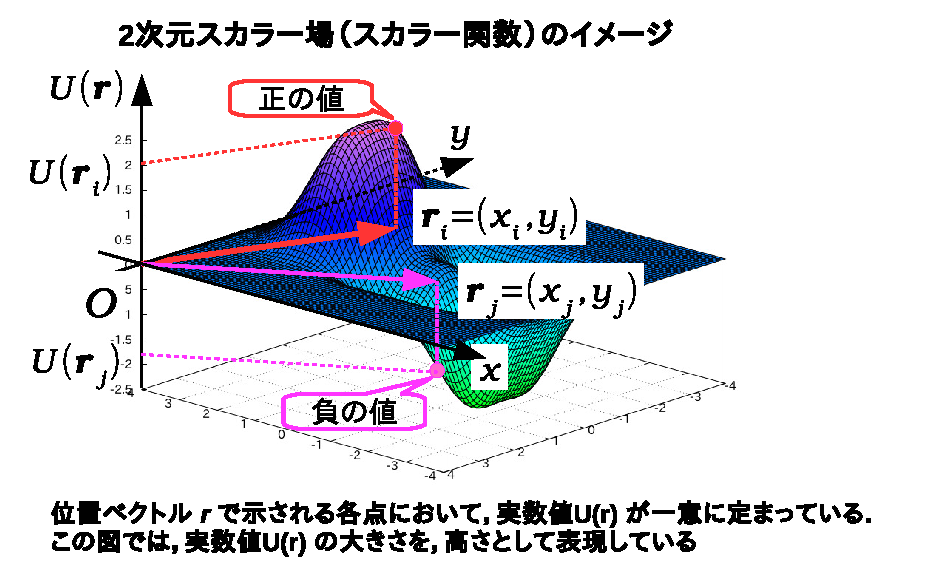
\includegraphics[keepaspectratio, width=7.2cm,height=6.64cm,clip]{scara_function_image001.pdf}
                            \caption{二次元のスカラー関数のイメージ}
                            \label{fig:scara_function_image001}
                        \end{center}
                    \end{figure}


                ポテンシャル$\cdot$エネルギーには地表付近の重力による
                位置エネルギー $mgh$ のほかに,もっと一般的な
                万有引力による位置エネルギーとか,
                電気的なポテンシャル$\cdot$エネルギーがある.
                ポテンシャル$\cdot$エネルギーといった時はこれらを総称していう時もあり,
                注意が必要である.
            \end{mysmallsec}

            \begin{mysmallsec}{運動エネルギーの定義}
                運動エネルギー $T$ についても,改めて定義する.
                    \begin{myshadebox}{運動エネルギーの定義}
                        運動エネルギー $T$ を,次式で定義する.
                        \begin{align}
                        T := \frac{1}{2}mv^{2}
                        \end{align}
                    \end{myshadebox}

                なぜ運動エネルギーというかについては,
                この式がエネルギーの単位をもち,かつ,速度だけによって
                その値が決まるからと考えればよいと思う.
            \end{mysmallsec}

            \begin{mysmallsec}{エネルギー関数 $E$ の独立変数}
                運動エネルギーは速度の関数として捉えられる
                    \footnote{
                        上で運動量表示もできることを示したが,ここでは速度表示の運動エネルギーを
                        考える.
                    }.
                これを,$T=T(\dot{\br})$ と表す.
                また同様に,ポテンシャル$\cdot$エネルギーは位置座標の関数として捉えることができ,
                これを $U=U(\br)$ と書く.
                従って,力学エネルギーは速度と位置の関数である考えられる.なぜなら,
                \begin{align}
                E(\dot{\br},\,\br)=T(\dot{\br})+U(\br)
                \end{align}
                と書けるからである.
            \end{mysmallsec}

            \begin{mysmallsec}{エネルギー保存則}
                さて,力学的エネルギー保存の法則を式(\ref{b})のように書いても
                よいが,「保存則」というからには,時間に依存していないということを
                式で表現しておきたい.そこで,上式の力学的エネルギー $E$ を時間微分して,
                その結果が 0 であるというように表現する形に書き換えておく.
                            \begin{myshadebox}{力学的エネルギー保存の法則}
                                力学的エネルギー保存の法則は,次式によって表される.
                                \begin{align}
                                    \frac{\df E}{\df t}=0
                                \end{align}
                            \end{myshadebox}

                このように考えられる理由は,物体の運動エネルギーとポテンシャル$\cdot$エネルギーの和 $E$ が
                時間変化しないという前提があるからである.
                物体の運動エネルギーと位置エネルギーが時間変化するとき,
                すなわち,$T=T(\dot{\br},\,t)$,$U=U(\br,\,t)$ であるとき
                は,一般には保存則は成り立たない.物体のエネルギーが時間変化するということは,物体は外か
                ら仕事を受けてエネルギーをもらう(とられる)からである.仕事とは外力が引き起こすものであり,
                つまり,「物体に外力が働くときには,力学的エネルギー保存の法則は成り立たない」とい
                える.式で書けば以下の通り.

                この場合の力学的エネルギーは時間 $t$ を変数に含み,
                \begin{align}
                E(\dot{\br},\,\br,\,t)
                =T(\dot{\br},\,t)+U(\br,\,t)
                \end{align}
                と書かれる.時間 $t$ で微分すると,
                \begin{align*}
                \frac{\rd E(\dot{\br},\,\br,\,t)}{\rd t}
                &=\frac{\rd }{\rd t}\biggl\{ T(\dot{\br},\,t)+ U(\br,\,t)\biggr\} \\
                &=\frac{\rd T(\dot{\br},\,t)}{\rd t}+\frac{\rd U(\br,\,t)}{\rd t}
                \end{align*}
                この式の最右辺は0ではなく,時間 $t$ を変数に含む関数である.これを
                簡単に $\alpha (\dot{\br},\,\br,\,t)$ と
                書くことにしよう.すると式は,
                \begin{align}
                \therefore \quad
                \frac{\rd E(\dot{\br},\,\br,\,t)}{\rd t}
                =\alpha (\dot{\br},\,\br,\,t)
                \end{align}
                というように,エネルギー保存則の時間微分は,時間に依存することがはっきりとわかる.

                この関数 $\alpha (\dot{\br},\,\br,\,t)$ の具体的な形は,
                運動エネルギーとポテンシャル$\cdot$エネルギーが
                どのように時間に依存しているかによる.
                この関数 $\alpha(\dot{\br},\,\br,\,t)$ が
                物体のエネルギーの変化量である.

                従って \textbf{外力が物体に働くとき,力学的エネルギーは
                保存しない} ということになる.しかし,もっと広く考えて,外力を含んだ系を
                考えるならば,エネルギーは保存している.これを \textbf{エネルギー保存の法則} という.
                この法則は経験的事実によって,与えられる法則であり,この法則が破られた現象は
                ないとされる.
                (この場合,力学的エネルギーが保存するわけではない.
                外力によって生じた熱力学的エネルギーや電磁気的エネルギーのことをいう.)
            \end{mysmallsec}

            \begin{mysmallsec}{まとめ}
                説明が長くなってしまったが,以上によって,ニュートンの運動方程式から,
                力学的エネルギー保存の法則を導いたことになる.整理しよう.
                まず,ニュートンの運動方程式を認めた($m\textit{\textbf{a}}=\bF$).これは
                力学の出発点となる方程式である.その次に,
                仕事という概念を導入し($W=\bF\cdot \Delta \textit{\textbf{s}}$),
                そこから力学的エネルギーという概念を,運動エネルギーと位置エネルギーの
                2種類のエネルギーの和であると定義した($E=T+U$).そして,
                力学的エネルギーは時間によらず一定値を保つことを
                発見した.

                従って,ニュートンの運動方程式から,
                力学的エネルギー保存の法則を見出したことになる.
            \end{mysmallsec}

            \begin{memo}{注意}
                但し,この $\bF$ は \textbf{保存力} であるとして
                いることを忘れてはならない.
                保存力については後の\ref{PF}で確認することだが,
                ここでは,「力のする仕事が経路によらず,始端と終点
                によってだけ決定されるならば,この力は保存力である」
                と考えてもらいたい.
            \end{memo}


%       %======================================================================
%       %  SubSection
%       %======================================================================
        \subsection{万有引力によるポテンシャル$\cdot$エネルギー}
            ポテンシャル$\cdot$エネルギーの定義を得たので,それを具体的に計算してみる.その例として,
            万有引力によるポテンシャル$\cdot$エネルギーを考える.
            ただ単に,ポテンシャル$\cdot$エネルギーの定義
            式(\ref{eq:PE})に,万有引力を代入すればよいだけである.では,
            早速計算する.

            万有引力は,式(\ref{Grav})によって
                \begin{align}
                    \bF_{\rm{AB}}
                    = -G\frac{m_{\rm{A}}m_{\rm{B}}}{{\left| \br_{A}
                    -\br_{B} \right|}^{2}}
                    \frac{\br_{A}-\br_{B}}{\left| \br_{A}
                    -\br_{B} \right|}
                \end{align}
            と書かれた.ここでは, 質量 $m_{\rm{A}}$ によるポテンシャル$\cdot$エネルギーを考える.
            式変形が煩雑にならないように,
                \begin{align*}
                \br:=\br_{A}-\br_{B}
                \end{align*}
            とおく.
                \begin{align}
                    \bF_{\rm{AB}}
                    = -G\frac{m_{\rm{A}}m_{\rm{B}}}{{\left| \br \right|}^{2}}
                    \frac{\br}{\left| \br \right|}
                \end{align}
            これを,ポテンシャル$\cdot$エネルギーの定義式(\ref{eq:PE})に代入すると,
                \begin{align}
                    U&=-\int \bF_{\rm{AB}}\cdot \df\br  \notag \\
                     &=\int G\frac{m_{\rm{A}}m_{\rm{B}}}{{\left| \br \right|}^{2}}
                    \frac{\br}{\left| \br \right|} \cdot \df\br \notag \\
                     &=Gm_{\rm{A}}m_{\rm{B}}\int \frac{1}{\left| \br \right|^{2}}\df\br \notag \\
                     \therefore \quad U
                     &=-Gm_{\rm{A}}m_{\rm{B}}\frac{1}{\left| \br \right|}
                \end{align}
            と計算される.
            $\br:=\br_{A}-\br_{B}$ を思い出せば,次のようになる.
                \begin{myshadebox}{重力ポテンシャル}
                    重力ポテンシャルは次式で定義される.
                    \begin{align}\label{eq:Grav_1}
                        U=-G\frac{m_{\rm{A}}m_{\rm{B}}}{\left| \br_{A}-\br_{B}\right|}
                    \end{align}
                \end{myshadebox}

            この式(\ref{eq:Grav_1})が質量 $m_{\mathrm{A}}$ が
            その周りに生じさせるポテンシャル$\cdot$エネルギーである.
            このようなポテンシャルを \textbf{重力ポテンシャル} いう.

%       %======================================================================
%       %  SubSection
%       %======================================================================
        \subsection{保存力}\label{PF}
                    今までは,力の存在を仮定して,エネルギーを考えていた.しかし,あくまで仮定しているだけであって,
                    決してはっきりとした概念ではない.ならば逆に,エネルギーを仮定して
                    力を導くことを考えてもよいだろう.
                    力とエネルギーのどちらを基礎とするかは,
                    理論がスマートになる方をとるべきだ.
                    エネルギーを仮定して,力を導出する方が現代的な考え方である.
                    ポテンシャル$\cdot$エネルギーの定義式を力 $\bF$ について
                    解く.$\bF=\left( F_{x}, F_{y},F_{z}\right)$ とする.
                    また,$\df\br=\left( \df x ,\df y ,\df z \right)$ とする.
                        \begin{align}
                            U &= -\int \bF\cdot \df\br \notag \\
                              &= -\int \left( F_{x}\df x+F_{y}\df y+F_{z}\df z \right)
                        \end{align}
                    ここで,$\rd U/\rd x$ を計算すると,
                        \begin{align}
                            \frac{\rd U}{\rd x}=-F_{x}
                        \end{align}
                    となる.ここで記号 $\rd U/\rd x$ の $\rd/\rd x$ は,
                    ($U$ を)“$x$ について微分する”ということである.その際,その他の変数($y$,$z$)は
                    定数とみなすと約束する.$x$ 方向の関数の変化度を知りたいときに,
                    用いる概念である.このような微分の仕方を \textbf{偏微分} という.

                    $y$,$z$ 方向についても同様に考えて,
                        \begin{align}
                        \frac{\rd U}{\rd y}&=-F_{y} \\
                        \notag \\
                        \frac{\rd U}{\rd z}&=-F_{z}
                        \end{align}
                    以上より,
                        \begin{align}\label{hozonryoku}
                            \left( \frac{\rd U}{\rd x} , \frac{\rd U}{\rd y},
                            \frac{\rd U}{\rd z}\right)
                            &=\left( -F_{x} , -F_{y} ,-F_{z} \right) \notag \\
                            \therefore \quad \bF
                            &=-\left( \frac{\rd U}{\rd x} ,
                            \frac{\rd U}{\rd y},
                            \frac{\rd U}{\rd z}\right)
                        \end{align}
                    を得る.ここで,次の微分演算子を定義する.
                        \begin{align}
                        \dgrad:= \left( \frac{\rd}{\rd x} , \frac{\rd}{\rd y},
                        \frac{\rd}{\rd z}\right)
                        \end{align}
                    (この記号の図形的なイメージは次項目で説明する.ここでは
                    とりあえず,記号として受けいれてほしい.)

                    この微分演算子は,$U$ の $x$,$y$,$z$ の3方向の傾きを求める演算子である.つまり,
                    空間の \textbf{勾配}
                        \footnote{
                            「勾配」とは,
                            面の傾斜の度合いのことをいう.例えば,道路の坂
                            が急であるとき,「この坂は急勾配である」といった使い方がされる.
                        }
                    を求める演算子と言える.$\dgrad$ を「グラディエント」と読む.
                    式(\ref{hozonryoku})を
                        \begin{align}
                            \bF=-\left( \frac{\rd}{\rd x} ,
                            \frac{\rd}{\rd y},
                            \frac{\rd}{\rd z}\right)U
                        \end{align} と変形する.そして,$\dgrad$ を
                    用いて,\\
                            \begin{align}
                                \bF=-\mathrm{grad\,} U
                            \end{align}
                    と書ける.
                    この式より,ポテンシャル$\cdot$エネルギーを仮定して力を導出するという意味として捉え直せる.

                    なので,ここで思い切って,保存力が生じている理由は,その周囲にポテンシャルエネルギーがあるからである,
                    と考えなおそう.保存力がポテンシャルエネルギーを周囲に作るというイメージよりも,そもそも最初は
                    ポテンシャルエネルギーがそこにあり,我々は,ポテンシャルエネルギーそのものを見ることはできないが,
                    その一端を保存力として観測していると考える方が,自然である.力を仮定してポテンシャルエネルギーを
                    導く場合には,試験用の質点を用意して至るところに置き,ポテンシャルエネルギーの分布を得るとになる
                        \footnote{
                                保存力を線積分するイメージ.
                        }.
                    しかし,ポテンシャルエネルギーを仮定すれば,ポテンシャルエネルギーの勾配($\dgrad$)を取るだけで,
                    保存力がえられるのだ.

                    こう考えなおすと,保存力 $\bF$ は,以下のように,ポテンシャルエネルギー $U(\br)$ の勾配で与えられる.
                        \begin{align*}
                                \bF = -\dgrad U(\br) = -\frac{\rd U(\br)}{\rd \br}.
                        \end{align*}
                                        両辺を始点 ${\br}_{\mbox{a}}$ から終点 ${\br}_{\mbox{b}}$ で積分すると,
                        \begin{align}\label{eq:forceF_and_potentialU}
                                   \int_{\br_{\mbox{a}}} ^{\br_{\mbox{b}}}\bF \cdot \br
                                   &=    \int_{\br_{\mbox{a}}} ^{\br_{\mbox{b}}}
                                           \left(
                                                -\frac{\rd U(\br)}{\rd \br}
                                           \right) \notag \\
                                   &=  - \int_{\br_{\mbox{a}}} ^{\br_{\mbox{b}}} \df U(\br) \notag \\
                                   &=  - \left( U(\br_{\mbox{b}}) - U(\br_{\mbox{a}}) \right) \notag \\
                                   &=  - U(\br_{\mbox{b}}) - ( - U(\br_{\mbox{a}}) ) \notag \\
                                   &=  \mbox{(一定)}
                        \end{align}
                    最初の位置 $\br_{\mbox{a}}$ でのポテンシャルエネルギー $-U(\br_{\mbox{a}})$ と移動後の位置 $\br_{\mbox{b}}$ の
                    ポテンシャルエネルギー $-U(\br_{\mbox{b}})$ の差のみで表せるという結果を得た.つまり,経路に依存していない.
                    どのような経路をとっても,始点と終点を指定するだけで,線積分が計算できるのだ,この線積分は位置と力の内積に
                    関するものであり,すなわち,始点から終点までになした仕事にほかならない,とどのつまり,の式は,
                    物体を $\br_{\mbox{a}}$ から $\br_{\mbox{b}}$ まで移動させるのに必要なエネルギーを表しているということだ.

                                        ただこのままでは,位置 $\br$ のポテンシャルエネルギーを $-U(\br)$ と書いた場合,終点は $-U(\br)$ だが始点が
                                        定まっていないため,値が定まらない.そこで,基準点を設けて,それに対するポテンシャルエネルギーを定義しよう.

                                        一般に,$A-B$ という式を見た場合,$A$ は $B$ を基準とした値であると解釈できる.例えば,$A=5$,$B=3$ とした時,
                                        $A-B=2$ であり,$A$ は絶対値5だけど $B$ から見ればその差は2である.
                                                \footnote{
                                                        このような見方を,$B$を基準にしてみると表現する
                                                }.
                                    同様に,$- U(\br_{\mbox{b}}) - ( - U(\br_{\mbox{a}}) )$ は $- U(\br_{\mbox{a}})$ を基準にしたときの,
                                    $- U(\br_{\mbox{b}})$ の値と解釈できる.そこで,$- U(\br_{\mbox{a}})=0$ となるような点
                                        \footnote{
                                                このような点が現実にあるわけでない.人間が勝手に基準となる点を設定しなければいけない.$- U(\br_{\mbox{a}})=0$ と
                                                できる点を適宜用意する必要がある.多くの場合は,無限遠点を基準点に取ることが多い.無限遠点とは,これまた曖昧な
                                                概念だが,ここから遠ざかって見えなくなった先の更に先というイメージで十分だ.
                                                実際,無限遠点はここだと示すことはできず,想像するより他にない.問題によっては基準点を別の点にとったほうが
                                                計算しやすい場合がある.その場合は,基準点を最も計算しやすい適切な点に再設定すれば良い.どうせ基準点は計算結果に
                                                影響しないのだから(基準点を決めないと不定積分になり不定性が残るが,基準点があれば定積分となり不定性はなくなる).
                                        }
                                    を基準点にとると,定義する.
                                    こうすることで,始点を暗黙裏に仮定することにより,毎回基準点を示すことなく,ポテンシャルエネルギーを考えることができる.
                                    ただ,基準点を示さないのが当たり前になってくると,ポテンシャルエネルギーがそもそも基準点をとるということを忘れがちであるので,
                                    この点は注意が必要だ
                                        \footnote{
                                                簡略化した記述は効率的だが,記述しないがゆえに見えなくなってしまうというジレンマがある.
                                                慣れれば(当たり前になれば)当然のこととして捉えられるが,なかなか難しい.
                                        }.
                                    このように,より簡略化した記述では,ポテンシャルエネルギーと保存力の関係式は以下のようになる
                                        \footnote{
                                                まず,式(\ref{eq:forceF_and_potentialU})で,始点は $-U(\br_{\mbox{a}})=0$ となる基準点を選ぶのであった.
                                                また,終点 $-U(\br_{\mbox{b}})$ の添字 $\mbox{b}$ も明示しなくても,常に終点を示すものであると読み取ることが可能なので,
                                                記述省略してしまおう.
                                        }.
                        \begin{align*}
                                   \int \bF \cdot \br  =  - U(\br)
                        \end{align*}

                    一般には,全ての力がポテンシャル$\cdot$エネルギーから導出されるわけではない.つまり,非保存力であるものもある.
                    この場合には,非保存力 $\bar{\bF}$ のする仕事を $W$ として,
                        \begin{align}
                            \bar{\bF}
                            = -\frac{\rd W}{\rd\br}
                        \end{align}
                    と書ける.もちろん,保存力と非保存力の両方を含む場合は,力の重ね合わせの原理から,
                        \begin{align}
                            \bF+\bar{\bF}
                            = -\frac{\rd U}{\rd\br}
                              -\frac{\rd W}{\rd\br}
                        \end{align}
                    である.
                    \begin{figure}[hbt]
                        \begin{center}
                            \includegraphicslarge{hozonryoku.pdf}
                            \caption{重力から受ける仕事は鉛直方向のみ}
                            \label{fig:hozonryoku}
                        \end{center}
                    \end{figure}

%       %======================================================================
%       %  SubSection
%       %======================================================================
        \subsection{勾配}
                    演算子 $\dgrad$ は,以下のように定義される量であることを,
                    前項目で確認した.
                        \begin{align}
                        \dgrad:= \left( \frac{\rd}{\rd x} , \frac{\rd}{\rd y},
                        \frac{\rd}{\rd z}\right)
                        \end{align}
                    この定義式をイメージすることが,この項目の目標である.

                    唐突ではあるが,
                    まず,連続でなめらかな1変数関数 $f_{1}=f(x)$ のグラフの接線の傾き $f'_{1}$ 考える.
                    $f'_{1}$ は $f_{1}$ の $x$ に関する微分であり,
                    \begin{align}
                    f'_{1}=\frac{\df }{\df x}f_{1}
                    \end{align}
                    のように与えられる.(図\ref{fig:grad1}参照)
                    これが1変数関数の場合である.

                \begin{figure}[hbt]
                    \begin{tabular}{cc}
                        \begin{minipage}{0.5\hsize}
                                    \begin{center}
                                        \includegraphicsdouble{grad1.pdf}

                                        (A) 1変数関数
                                        \label{fig:grad1}
                                    \end{center}
                        \end{minipage}
                        \begin{minipage}{0.5\hsize}
                                    \begin{center}
                                        \includegraphicsdouble{grad2.pdf}

                                        (B) 2変数関数
                                        \label{fig:grad2}
                                    \end{center}
                        \end{minipage}
                    \end{tabular}

                        \caption{傾き}
                \end{figure}

                    この考えを,
                    2変数関数 $f_{2}=f_{2}(x,\,y)$ の場合について拡張してみる.
                    関数 $f_{2}=f_{2}(x,\,y)$ は図\ref{fig:grad2}のように
                    描くことができる.もちろん,関数 $f_{2}=f_{2}(x,\,y)$ は連続で
                    なめらかであることを仮定している.関数 $f_{2}=f_{2}(x,\,y)$ を,
                    点$(x,\,y)$ を代入したときの高さを表していると考えれば,
                    このような点を全て集めると,
                    それは\textbf{曲面}をなしていると言える
                        \footnote{
                            つまり,$f(x,\,y)$ は幾何学的には,曲面を表す関数としてイメージされる.
                        }.
                    1変数関数における曲線が,
                    2変数関数になると,曲面になるのである.
                    従って,2変数の場合には,
                    直線の接線の傾きを考えるのでは不十分であり,
                    面の \textbf{勾配} を考えなければいけない
                        \footnote{
                                「勾配」とは面の傾き具合を表す語彙.1次元の場合は「傾き」という
                                表現を使ったが,2次元の場合は「勾配」と言い表す.2次元以上の場合
                                でも「勾配」という.
                        }.
                    そこで,図\ref{fig:grad2}の青い線で描いたような,
                    接面の勾配を考えるのである.この接面の勾配を考える.
                    図\ref{fig:grad2}では説明しにくいので,改めて,
                    図\ref{fig:grad3}に必要な部分だけ書き改めることにする.
                    (若干異なっているが許してほしい.)

                \begin{figure}[hbt]
                    \begin{tabular}{cc}
                        \begin{minipage}{0.5\hsize}
                                    \begin{center}
                                        \includegraphicsdouble{grad3.pdf}

                                        (A) 2変数関数の傾き
                                        \label{fig:grad3}
                                    \end{center}
                        \end{minipage}
                        \begin{minipage}{0.5\hsize}
                                    \begin{center}
                                        \includegraphicsdouble{grad4.pdf}

                                        (B) 接面の勾配
                                        \label{fig:grad4}
                                    \end{center}
                        \end{minipage}
                    \end{tabular}

                        \caption{面の傾き}
                \end{figure}

                図の緑の太線で示した曲面部分に接する平面を
                考える.図の $A$ は $x$--$y$ 平面上の点を表している.そのような平面のことを \textbf{接面} と
                いうことにする.この接面の勾配を
                示すには,$x$ 方向の接面の傾きと,$y$ 方向の
                接面の傾きを考えればよい.従って,それぞれの方向に \textbf{偏微分} すればよい.
                前項目では偏微分の定義には触れなかったので,
                ここでは簡単に偏微分の定義式を示しておこうと思う.

%       %======================================================================
%       %  SubSection
%       %======================================================================
        \subsection{保存力と $\dgrad$ の図的イメージ}
                偏微分は,グニャグニャ曲がっている面のある一点における
                傾きを計算する場合に役に立つ.面の傾きを考えるには,
                2つの方向の傾きを考える必要がある.しかし,2方向の傾き
                を同時に考えることは難しい.そのため,一方向ずつ傾きを
                計算する.一方向の傾きを計算するには,曲線の傾きと
                同じように考えられる.そのとき,残りのもう1方向は定数として
                扱う.

                例えば,接面の $x$ 方向の傾きを考える場合,$y$ 座標を一時的に固定して定数と
                して扱い,$x$ 方向のみに着目し微分する.偏微分の記号は通常の微分と区別するために,
                $\rd$ という文字が使われる.具体的には,以下の通り.
                \begin{align}
                    \frac{\rd }{\rd x}f(x,\,y) := \lim_{\Delta x \to 0} \frac{f(x+\Delta x,\, y) - f(x,\,y)}{\Delta x}.
                \end{align}

                接面の $x$ 方向の傾きも同様に考えて,
                \begin{align}
                    \frac{\rd }{\rd y}f(x,\,y) := \lim_{\Delta y \to 0} \frac{f(x,\,y+\Delta y) - f(x,\,y)}{\Delta y}.
                \end{align}

                これらを用いて,曲面f上の点($x,\,y$)の接面は
                    \begin{equation*}
                        \left( \frac{\rd }{\rd x}f(x,\,y) \,,\; \frac{\rd }{\rd y}f(x,\,y) \right)
                    \end{equation*}
                と表現できる.ただ,$f$ の独立変数をいちいち書いていると煩雑なので,省略する場合が多い
                    \footnote{
                        偏微分の対象となる方向は分母でわかるし,他の変数は定数扱いなので無理して明示する必要もない.
                        問題になるとしたら,独立変数の個数がわからなくなってしまうことだが,前もって明記しておけば
                        覚えていられるだろう.
                    }.
                    \begin{equation*}
                        \left( \frac{\rd }{\rd x}f \,,\; \frac{\rd }{\rd y}f \right)
                    \end{equation*}
                もっと省略して,以下のように書かれることもある($f$ をカッコの外に出した).
                    \begin{equation*}
                        \left( \frac{\rd }{\rd x} \,,\;  \frac{\rd }{\rd y} \right) f
                    \end{equation*}
                こうすると,式に意味を与えやすい
                    \footnote{
                        ただし,注意したいのは,
                        $\displaystyle \left( \frac{\rd }{\rd x} \,,\; \frac{\rd }{\rd y} \right)$ と $f$ の積
                        と解釈してはいけない,ということである.
                    }.
                こうすると,表現上,$f$ に対して
                操作 $\displaystyle \left( \frac{\rd }{\rd x} \,,\; \frac{\rd }{\rd y} \right)$ を施すことで,
                接面が現れると読むことができる.物理学では,
                    \begin{equation*}
                        \dgrad := \left( \frac{\rd }{\rd x} \,,\; \frac{\rd }{\rd y} \right)
                    \end{equation*}
                として,単に
                    \begin{equation*}
                        \dgrad f
                    \end{equation*}
                と書かれる.ポテンシャルエネルギーを考える場合には,$f=-U(\br)$ とすればいい.

                    ポテンシャルエネルギーの関数 $U(\br)$ が与えられている時,保存力 $\bF(\br)$ は以下のように計算できる.
                    \begin{align*}
                        \bF (\br) &= - \dgrad U(\br) \\
                                  &= -\left(
                                                \frac{\rd}{\rd x}\,,\;
                                                \frac{\rd}{\rd y}\,,\;
                                                \frac{\rd}{\rd z}
                                     \right)  U(\br) \\
                                  &=  \left(
                                        - \frac{\rd U(\br)}{\rd x}\,,\;
                                        - \frac{\rd U(\br)}{\rd y}\,,\;
                                        - \frac{\rd U(\br)}{\rd z}
                                     \right)
                        \end{align*}

                上式で表されるポテンシャルエネルギーと保存力のイメージを,以下に表現しておこう.
                    \begin{figure}[hbt]
                        \begin{center}
                            \includegraphicslarge{scara_function_image002.pdf}
                            \caption{ポテンシャルエネルギーと保存力}
                            \label{fig:sensekibun_shukaisekibun_002}
                        \end{center}
                    \end{figure}

                この図で注意してみて欲しいのは,ポテンシャルエネルギーを2次元で表していることである.
                実際の空間はは3次元だが,これだと図に表すことができない
                        \footnote{
                            関数の取る値をグラフで示すための次元が1つ必要になるからである.
                            ここでは,本来の3次元の内から1次元減らし,代わりに関数のとる
                            値を山として表現している.
                        }.

%       %======================================================================
%       %  Memo
%       %======================================================================
        \begin{memo}{$\rd / \rd \br$ という表現について}
            上で使ってしまったが,便利でよく使われてしまう表現に,
                        \begin{equation*}
                                \frac{\rd f(\br)}{\rd \br}
                        \end{equation*}
            というものがある.

            ベクトル $\br$ で割り算しているように見えるが,そうではない
                \footnote{
                    "ベクトル除算" なんてものはない.
                }.
            本当は,
                        \begin{align*}
                                \frac{\rd f(\br)}{\rd \br}
                                &=
                                    \left(
                                      \frac{\rd f(\br)}{\rd x} \,,\;
                                      \frac{\rd f(\br)}{\rd y} \,,\;
                                      \frac{\rd f(\br)}{\rd z}
                                \right) \\
                                &=
                                    \left(
                                      \frac{\rd f(x,\,y,\,z)}{\rd x} \,,\;
                                      \frac{\rd f(x,\,y,\,z)}{\rd y} \,,\;
                                      \frac{\rd f(x,\,y,\,z)}{\rd z}
                                \right)
                                \end{align*}
                    という意味で使われるものである.紛らわしいが,よく見かける表現なので注意しておきたい.
                    こういう表現は,疑問や誤解を招くので,避けたほうが良い
                        \footnote{
                            勾配演算子 $\dgrad$ や後で紹介する数学記号 $\nabla$ を使って表現すべき.
                        }.
        \end{memo}

%       %======================================================================
%       %  SubSection
%       %======================================================================
        \subsection{保存力と周回積分}\label{subsec:hozonryoku_to_shukaisekibun}
                        ポテンシャルエネルギー $U(\br)$ のみの場合などのように,外力が働かない時,
                        始点Aと終点Bの2つの位置ベクトルを定めると,AからBまでの経路Cは無数に存在するが,
                        AからBまで物体を移動させる仕事はその経路に依存せず,一定値をとる.
                        \begin{equation*}
                                \oint_{\mbox{C}} \bF (\br) \cdot \df \br = U(\br_{\mbox{b}}) - U(\br_{\mbox{a}}).
                        \end{equation*}
                        このような性質を持つ関数で表される力のことを,\textbf{保存力} と言うことはすでに記述した.
            特に注目すべきはことは,B$=$Aとした時(始点と終点を同じ点にした場合),
                        \begin{equation*}
                                \oint_{\mbox{C}} \bF (\br) \cdot \df \br = U(\br_{\mbox{a}}) - U(\br_{\mbox{a}}) = 0
                        \end{equation*}
                        となることである.


                        ポテンシャルエネルギー値 $U(\br)$ がベクトル $\br$ に対して一意に定まる場合,
                        $U$ により生じる力は保存力となる.
                    \begin{figure}[hbt]
                        \begin{center}
                            \includegraphicslarge{sensekibun_shukaisekibun_001.pdf}
                            \caption{保存力の性質}
                            \label{fig:sensekibun_shukaisekibun_001}
                        \end{center}
                    \end{figure}


                        しかし,例えば下図のように,ポテンシャルエネルギー値 $U(\br)$ がベクトル $\br$ に対して
                        一意に\textbf{定まらない}場合,$U$ により生じる力は保存力ではない.
                    \begin{figure}[hbt]
                        \begin{center}
                            \includegraphicslarge{sensekibun_shukaisekibun_004.pdf}
                            \caption{保存力でない場合}
                            \label{fig:sensekibun_shukaisekibun_004}
                        \end{center}
                    \end{figure}

%   %==========================================================================
%   %  Section
%   %==========================================================================
    \section{エネルギーと運動量}
        エネルギーと運動量は似たような概念だ.この2つの間には大切な関係がある.
        特に,量子力学を学習するとこの関係が顕著に現れてくる.
        運動量 $\bp$ をもつ物体に関与する力を保存力とし,$\bF$ とする.
                \footnote{
                        ここでは保存則について考えているのであった.保存力以外の外力が
                        働く場合は,運動量保存則とエネルギー保存則は成立しないの.
                }.
        運動量表示の運動方程式は
                        \begin{align*}
                        \frac{\df \bp}{\df t} = \bF.
                        \end{align*}
        であった.$t$ は時間である.
        ところで,保存力である $\bF$ はポテンシャルエネルギー $U(\br)$ を導入すると,
                        \begin{align*}
                        \bF = -\frac{\rd U}{\rd \br}.
                        \end{align*}
        ここで,$E(\br)=-U(\br)$ と置いてしまおう.
                        \begin{align*}
                        \bF = \frac{\rd E}{\rd \br}.
                        \end{align*}
                要するに,$\rd U/\rd \br$ と $\rd E/\rd \br$ は共に力の次元を持っている,
                $\bF$ を消去して,それぞれの次元を考えると,
                        \begin{align*}
                        \left[\frac{\df \bp}{\df t}\right] = \left[\frac{\rd E}{\rd \br}\right]
                        \end{align*}
                微分記号と偏微分記号は不要.
                        \begin{align*}
                        \frac{[\bp]}{[t]} = \frac{[E]}{[\br]}
                        \end{align*}
                これを以下のように書きなおす.
                        \begin{align}
                                [\bp] \cdot [\br] = [E][t].
                        \end{align}
            もしかしたら,$\br=(x,\,0,\,0)$,$\bp=({p}_{x},\,0,\,0)$ としたほうがわかりやすいかもしれない.
                        \begin{align*}
                                {p}_{x}x = Et.
                        \end{align*}



\chapter{座標変換}
%   %-----------------------------------------------------------------------------------------------
%   %  Input
%   %    File Name : PhysNote_CM_Zahyou.tex
%   %    説明      : 座標について記述する
%   %-----------------------------------------------------------------------------------------------
        \section{座標のとりかた}
\subsection{座標とは}
    空間内の点の位置を指定する手段として,\textbf{座標} はとても重要であり,
    座標なくしては位置を数学的に表すことはできない
        \footnote{
            これ以上に簡潔なものはない,という意味で.
        }.
    今まで主に使ってきた座標は,縦・横・高さの3つの数字であらわされる,\textbf{3次元直交座標} を使っていた.
    しかし,点の位置を指定するのに,この座標系しか考えられないということはない.
    \textbf{3次元空間内の点を表すには,適当に決めた“3つの互いに独立な変数”を用いればよい}.
    座標の取り方は3次元直交座標以外にも,例えば,\textbf{極座標} とか,\textbf{斜交座標} が
    よく取り上げられる.座標によって位置の示し方は異なるが,異なるのは示し方だけであって,どの座標を採用しても
    示される位置に違いはない.極座標を使おうが斜交座標を使おうが,それらを使ってあらわされる位置の特性に
    違いが出るわけではない.

    下手な例えかもしれないが,座標の違いは言葉の違いに似ている.
    現象を英語で表現しようが,日本語で表現しようが,その表現される現象が
    変わるわけではない.ただ,同じ現象を日本語で説明された時と,
    英語で説明された時のイメージ(ニュアンス)は異なるように,
    採用する座標によって主張する部分が変わってくる.極座標は角運動(回転運動)
    を表現するのに簡潔であることが多く,惑星の運動やコマの回転運動などを扱うときは,
    極座標がよく用いられる.

    以下では,座標の種類をいくつか見た後,それらの相互の関係について,考える.
    座標の相互関係は \textbf{座標変換} とう考え方を使って表現される.
    座標変換によって,ある座標から別の座標へ切り替えることが可能になる.
    特に,相対性理論は,座標変換による計算地獄だ.
    ここでは,将来学習する相対性理論も視野に入れつつ,
    座標そのものに対するイメージを習得していこう.

\subsection{直交座標}
    \textbf{直交座標} については説明するまでもない.
    今まで考えてきた $x$,$y$,$z$ を直線軸とし,これらの軸が
    互いに直交するようにとった座標ののことである.
        \begin{figure}[hbt]
            \begin{center}
                \includegraphicsdefault{chokkou.pdf}
                \caption{直交座標}
                \label{fig:chokkou}
            \end{center}
        \end{figure}

\subsection{斜交座標}
    直交座標は各直線軸同士の交わりが,互いに直交していた.
    しかし,直交していない ----- つまり,斜めに交わっていても ,座標として成立する.
    直交していない直線軸で表される座標は \textbf{斜交座標} とよばれる.

    まず,2次元で考えてみよう.直交座標 $x\,$---$\,y$ と,斜交座標 $x'\,$---$\,y'$ の関係
    を考えてみよう.図を描けば図\ref{fig:shakou_chokkou_zahyou}のようになる.
        \begin{figure}[hbt]
            \begin{center}
                \includegraphicsdefault{shakou_chokkou_zahyou.pdf}
                \caption{斜交座標}
                \label{fig:shakou_chokkou_zahyou}
            \end{center}
        \end{figure}

    まず $x'$ を ,$x$ と $y$ で表現することを考えよう.つまり,直交座標 $x\,$---$\,y$ から見た,
    直線 $x'$ の式を考えるのである.直線の式は簡単に書くと,$y=ax+b$ である.$a$ は
    直線の傾きで,$b$ は直線が $y$ 軸と交わる切片である.直線の傾きを知るには,直線の式を
    微分ればよい.
        \begin{equation*}
            \mbox{(直線の傾き)} \; a = \frac{\df y}{\df x}.
        \end{equation*}
    また,今回は,簡単のために
        \footnote{
            「簡単のために」とは,説明が複雑にならないように,条件を簡単にして考えたいということである.
            一般的に考えてしまうと,それ説明するときに式が複雑になり,要点がつかみにくくなってしまう.
            簡単化してしまうと,一般的な議論ができない.しかし,要点をつかむことが大事であるので,
            一般的議論を犠牲にするのである.
        },
    $b=0$ としよう.すると,関係式は次のように簡単になってしまう.
        \begin{align}
            x ' \mbox{の式} : y = \frac{\df y}{\df x}x
        \end{align}

\subsection{極座標}
            極座標の場合の座標変数の取り方は,
            自分の位置する場所を座標原点 O としたとき,
            自分からの距離 $r$ と,水平方向のある1方向を基準にしたときの角度 $\phi$,
            そして,鉛直方向の上向きを基準としたときの角度 $\theta$ の3つの変数を用いる.
            図でイメージするならば図\ref{fig:kyoku2}のようである.但し,
            直交座標との対応関係がわかるように,直交座標も点線で描いている.

           図\ref{fig:kyoku2}のように,
            極座標の3つ独立な座標変数は $(r,\,\theta,\,\phi)$ で
            表現される.それらのとり方は,書いた通りである.
            これらの変数には一応名前がついており,$r$ を \textbf{動径},$\theta$ を \textbf{天頂角},
            $\phi$ を \textbf{方位角} という.
                    \begin{figure}[hbt]
                        \begin{center}
                            \includegraphicsdefault{kyoku2.pdf}
                            \caption{極座標}
                            \label{fig:kyoku2}
                        \end{center}
                    \end{figure}
                    \begin{figure}[hbt]
                        \begin{center}
                            \includegraphicsdefault{kyoku_chokkou.pdf}
                            \caption{直交座標との対応}
                            \label{fig:kyoku_chokkou}
                        \end{center}
                    \end{figure}


            直交座標との関係は,図より
                    \begin{align}
                            \begin{cases}\label{kyoku_chokkou}
                                x=r\sin\theta \cos\varphi \\
                                y=r\sin\theta \sin\varphi \\
                                z=r\cos\theta
                            \end{cases}
                    \end{align}
            となることがわかる.



\subsection{円筒座標}
            円筒座標の場合の座標変数の取り方を説明する.
            そのイメージを図\ref{fig:entou}に描いておくので,
            この図を参照しながら読んでほしい.まず,
            自分の位置する場所を座標原点 O とする.
            そして,この座標原点 O を含むような1つの平面を
            選ぶ.この平面の選び方は複数存在するが,
            そのうちの1つを任意に選ぶとする.図\ref{fig:entou}では $x-y$ 平面に相当する
            ものである.さて,示したい点 $\textit{\textbf{P}}$ から,
            先に指定した平面に垂線を引き,
            垂線の足を $H$ とする.ここでまず一つ目の座標 $z$ を,
            点 $\textit{\textbf{P}}$ から $H$ へ引いた線分の長さとする.
             $\rho$ については座標原点 O から,$x-y$ 平面に
            沿って点 $H$ まで引いた線分の長さというようにとる.
            残りの1つの変数,$\phi$ については,極座標の場合と同様なとり方をする.

            従って,円筒座標で点の位置を示したいときは,$(\rho,\,\phi,\,z)$ と
            いう座標を用いることになる.
                \begin{figure}[hbt]
                    \begin{center}
                        \includegraphicsdefault{entou.pdf}
                        \caption{円筒座標}
                        \label{fig:entou}
                    \end{center}
                \end{figure}


            直交座標との関係は,図より
                    \begin{align}
                            \begin{cases}\label{entou_chokkou}
                                x=\rho\cos\phi \\
                                y=\rho\sin\phi \\
                                z=z
                            \end{cases}
                    \end{align}
            となることがわかる.$z$ 座標は同じである.


\section{異なる座標同士の関係}
\subsection{座標による違い}
                1つの同じ物体(質量:$m$)の運動をみて,二人の観測者がその物体の運動方程式を
                正しく記述したとしよう.運動方程式を書くときには,どのような座標をとるかを
                決める必要がある.座標には,直交座標,極座標など,いろいろな
                表し方があるが,そのどれをとってもよい.

                さて,二人のがそれぞれ書いた運動方程式を比べてみるとき,
                使用した座標が違っていたとしよう.運動方程式の記述の仕方は
                ,使用する座標によって変わってしまう.しかし,2つの運動方程式
                が表す物体の軌跡は,正しく記述されているので,全く同じになるはずである.
                しかし,その関係は,一見してわかりにくいものになるだろう.

                例として,一方の運動方程式を直交座標でかかれたものとし,もう一方を
                極座標でかかれているとしよう.簡単のために,2次元で考え,さらに,
                物体に加わる力は保存力(ポテンシャルは $V(x,\,y)$)であるとしよう.
                直交座標で書かれた運動方程式は,
                    \begin{align}
                        \begin{cases}
                            \displaystyle m\frac{\df^{2} x}{\df t^{2}} = -\frac{\rd V(x,\,y)}{\rd x} \\
                            \displaystyle m\frac{\df^{2} y}{\df t^{2}} = -\frac{\rd V(x,\,y)}{\rd y}
                        \end{cases}
                    \end{align}
                である.同じ運動方程式を,極座標で表すと,
                    \begin{align}
                        \begin{cases}
                            \displaystyle m\biggl\{ \frac{\df^{2} r }{\df t^{2}}  - r\left( \frac{\df \theta}{\df t} \right)^{2} \biggr\}
                                    = -\frac{\rd V(r,\,\theta)}{\rd r} \\
                            \displaystyle m\left( r\frac{\df^{2} \theta }{\df t^{2}} + 2\frac{\df r}{\df t}\frac{\df \theta}{\df t} \right)
                                    = -\frac{1}{r}\frac{\rd V(r,\,\theta)}{\rd \theta}
                        \end{cases}
                    \end{align}
                となる.

                運動方程式を直交座標で表そうが,極座標で表そうが,
                結果として得られる軌道は全く変わらない
                    \footnote{
                        確かに,勝手に選択した座標によって運動方程式を記述しても,結果として
                        得られる物体の運動の軌跡は,1つである.これはこれで,大変驚くべき事だと思う.
                        しかし,不満もあるだろう.運動方程式の形が,座標系によって異なるのである.
                        人間が勝手に決めた座標系によって,運動方程式の形が違うのである.
                        実はこの不満は,解析力学を見てみることで,解決をすることである.
                        ここではしばらく我慢して,異なる座標同士の関係について見ていくことにしたい.
                    }.

                座標は人間が勝手に決められるもので,そのとり方はいろいろある.どの座標を選んでも
                運動の法則を満たし,同じ結果を得ることができる.となると,この座標同士の関係はどう
                なっているかが気になってこよう.

                座標のとり方には,色々な方法があることを確認した.
                次に,それぞれの関係をで考えてみよう.

                    \subsection{直交座標 $\rightarrow$ 斜交座標}
                         直交座標と斜交座標の関係を考えよう.これは,座標同士の関係の中で,
                         最も理解しやすいものである.そしてまた,この関係は物理学ではとても重要な
                         関係である.なので,この関係はどうしても理解したい.
                         感覚的に分かるように,できるだけ細かいステップを踏んで,
                         考えていこう.

\section{座標変換}
                今までは具体的な2つの座標同士の関係を見てきた.
                実用的には,これまでの具体的な関係式のほうが,役に立つ
                ことだろう
                    \footnote{
                        実際の現象を解決するに当たっては,式は具体的に
                        書かれているほうが,使いやすい.多くある関係式
                        から,使いやすい式を選択すればよい.
                    }.
                しかし,理論物理学の目指すところは,一般的に通用する式
                を記述することである.この目標を満足させるためには,任
                意の2つの座標間の,変換関係式を記述ればよい.今までのに
                得た,具体的な関係式を参照しながら,一般的に通用する関
                係式を導いてみよう
                    \footnote{
                        発見的方法で,一般の座標変換式を導くことになる.
                        この方法をとると,「どんな2つの座標系間でも必ず
                        成り立つかどうか」を示す必要が出てくる.しかし,
                        このノートではその証明は省略する.明らかに成立
                        することが,わかるだろうから.いや,面倒臭い
                        から.知りたい場合は,座標変換に関する数学の教
                        科書や,物理学の教科書を参照しよう.
                    }.

                \subsection{座標系の表現の仕方}
                    さて,任意の2つの座標系を文字で表さないといけない.
                    この2つの座標系をそれぞれ,$x$ 座標系と $X$ 座標系
                    のように,小文字と大文字で区別することにしよう.そし
                    て,座標変換を考えるには,基準とする座標系を$x$ 座
                    標系と $X$ 座標系のどちらかに設定すると楽である.
                    ここでは,$x$ 座標系を基準の座標系としよう.基準の
                    座標系とは,もちろん,私に対して静止している座標系
                    のことである.

\section{座標変換と運動方程式}

            \begin{mycomment}
            ある慣性系で,物体の運動方程式をたてる.そして,その慣性系とは別の慣性系に移り,同じ物体の運動方程式を立てたとき,
            その運動方程式は形を変えてしまうのだろうか.結論をいうと,形を変えないのである.それを説明していく.慣性系から
            別の慣性系に移ることを,\textbf{ガリレイ変換} という.ここでいう変換とは \textbf{座標変換} のことである.座標変換をする
            ということには,「物体の観測をする立場を変えてみる」といった意味がある.観測する立場というのは,例えば,
            別の速度(等速度)で運動している状況での観測とか,加速度運動している状況での観測とかということである.
            \end{mycomment}

\subsection{ガリレイ変換}
            ある慣性系 $S_{a}$ から別の慣性系 $S_{b}$ に移ることを,\textbf{ガリレイ変換} という.
            このガリレイ変換について考える.
            系 $S_{a}$ の速度を
            $\bv_{a}$ とし,系 $S_{b}$ の速度を $\bv_{b}$ とする.
            また,系 $S_{a}$ の位置を
            $\br_{a}$ とし,系 $S_{b}$ の位置を $\br_{b}$ とする.このとき,
            系 $S_{b}$ を系 $S_{a}$ から見たときの相対速度 $\textit{\textbf{V}}_{ba}$ は
                \begin{align}
                    \textit{\textbf{V}}_{ba}=\bv_{b}-\bv_{a}
                \end{align}
            である.系 $S_{a}$ も系 $S_{b}$ も両方とも等速直線運動しているので,$\textit{\textbf{V}}_{ba}$ も
            一定の値をとる.この式を
                \begin{align}
                    \bv_{a}=\bv_{b}+\textit{\textbf{V}}_{ba}
                \end{align}
            のように変形して,両辺に時間 $t$ を掛けることによって,
                \begin{align}
                    \bv_{a}t&=\bv_{b}t+\textit{\textbf{V}}_{ba}t \notag \\
                    \Leftrightarrow\br_{a}&=\br_{b}+\textit{\textbf{V}}_{ba}t
                \end{align}
            という式が成り立つ.($\bv_{a}t$,$\bv_{b}t$ は
            絶対静止系に対する位置である.)上式は系 $S_{a}$ の位置 $\br_{a}$ から見た式である.
            ここで物体の運動方程式を作って,$m(\df^{2}\br_{a}/\df t^{2})=\bF$ とする.
            このとき,系 $S_{b}$ から物体を見ると運動方程式がどうなるかを考える.
            別の慣性系に移って,系 $S_{b}$ の位置 $\br_{b}$ から見れば,
                \begin{align}
                    \br_{b}&=\br_{a}-\textit{\textbf{V}}_{ba}t
                \end{align}
            である.この式が,系 $S_{a}$ から系 $S_{b}$ に移ったときの \textbf{ガリレイ変換} を表現する式である.

            この $\br_{b}$ について,運動方程式をたてると,
             \begin{align}
                m\frac{\df^{2}\br_{b}}{\df t^{2}}
                &=m\frac{\df^{2}\br_{a}}{\df t^{2}}-m\frac{\df^{2}\textit{\textbf{V}}_{ba}t}{\df t^{2}} \notag \\
                &=m\frac{\df^{2}\br_{a}}{\df t^{2}} \notag \\
                &=\bF
            \end{align}
            \begin{align}
                \Leftrightarrow m\frac{\df^{2}\br_{b}}{\df t^{2}}=\bF
            \end{align}
            である.この方程式は $m(\df^{2}\br_{a}/\df t^{2})=\bF$
            と同じ形をしている.
            すなわち,系 $S_{a}$ から運動を見ようが,系 $S_{b}$ から運動を見ようが,
            運動方程式は全く同じ形になることがわかる.このことを,
            ニュートンの運動方程式は \textbf{ガリレイ変換に対して不変である} という.

            今までは2つの慣性系が両方とも,速度をもつとして考えてきたが,
            これら2つの慣性系のうちどちらか一方が静止している場合を
            考えても,このガリレイ変換の式が変わることはない.
            なぜならガリレイ変換は,慣性系間の相対速度が
            重要なのであって,それら慣性系の絶対的な速度には関係がないからである.
            そこで,以下では基準となる慣性系の速度を0として考える.

            以上のことを踏まえて,ガリレイ変換を以降で使いやすい形にまとめておく.
            \begin{myshadebox}{ガリレイ変換}
                慣性系 $S$ と,$S$ に対して速度 $\bv$ で等速直線運動している慣性系 $S'$ を考える.
                ここに慣性系 $S$ の速度を0とし,基準の慣性系とする.
                基準慣性系 $S$ の位置座標を $\br$ で表現し,$S'$ の位置座標を $\br'$ で表現する.
                このとき,これらの2つの慣性系 $S$,$S'$ の座標間には以下の関係がある.
                \begin{align}
                    \br' =  \br+\bv t
                \end{align}
                ここに $t$ は時刻を表現するものである.
            \end{myshadebox}

\subsection{加速度系における物体の運動}
                2つの直交座標系を用意する.
                これらの座標系に名前を付けて,
                それぞれ系 $S_{1}$,系 $S_{2}$ とする.系 $S_{1}$ は等速直線運動しているとする.
                両方の座標系の原点が一致したとき,時刻を $t=t_{0}$ とする.
                また,各系は自転しないとする.
                今から,\textbf{系 $S_{1}$ での物体の運動を,系 $S_{2}$ から見ることを考える}.
                系 $S_{2}$ は系 $S_{1}$ に対して正方向に動いているとする.
                この変換に重要なのは位置である.座標と位置は全く同じことである.
                 位置を得れば,それを時間微分することによって,速度を得ることができるし,
                さらに時間微分することによって,加速度を得ることができる.

                「加速度をもった座標系」の図で,$\br_{1}$ と$\br_{2}$ の関係を見てほしい.
                 $\br_{1}$ が系 $S_{1}$ から見たときの 物体の位置であり,
                 $\br_{2}$ が系 $S_{2}$ から見たときの物体の位置である.$\textit{\textbf{R}}$ は
                 系 $S_{1}$ から見た,系 $S_{2}$ の原点の位置である.もちろん,系 $S_{2}$ から系 $S_{1}$ の原点を
                 見るならば,$-\textit{\textbf{R}}$ となる.

                            \begin{figure}[htbp]
                                \begin{center}
                                    \includegraphicsdefault{gari1_fix.pdf}
                                    \caption{加速度をもった座標系}
                                    \label{fig:gari1}
                                \end{center}
                            \end{figure}

                「加速度をもった座標系」の図,以下の式が成り立つ.
                    \begin{align}
                        \br_{1}=\br_{2}+\textit{\textbf{R}}
                    \end{align}
                この式を,$\br_{2}$ での位置 $\br_{2}$ について解くと,
                    \begin{align}
                        \br_{2}=\br_{1}-\textit{\textbf{R}}
                    \end{align}
                となる.この座標 $\br_{2}$ について,質量 $m$ をもつ物体の運動方程式をたてると,
                    \begin{align}\label{kasokudo3}
                        m\frac{\df^{2}\br_{2}}{\df t^{2}}
                        &= m\frac{\df^{2}\br_{1}}{\df t^{2}}-m\frac{\df^{2}\textit{\textbf{R}}}{\df t^{2}}
                    \end{align}
                と変形される.すなわち,系 $S_{2}$ では,$-m(\df^{2}\textit{\textbf{R}}/\df t^{2})$ の
                力を受けれていることになる.

                ガリレイ変換との違いは,ガリレイ変換が慣性系から慣性系への変換であったのに対して,
                今度の変換は,慣性系から加速度系への変換である ということである.
                すなわち,$\textit{\textbf{R}}$ が
                加速度をもっているために,$-m(\df^{2}\textit{\textbf{R}}/\df t^{2})$ という力が
                生じてしまったのである.
                この力のことを,\textbf{見かけの力} という.

                見かけの力は普段の生活でも経験している.
                例えば,電車の中にいるとき,電車が動き始めるときや止まるときに
                「何か」に引っ張られる感覚がある.この「何か」が,見かけの力である.

                電車の中に固定された物体の動きを考える.
                電車の外にいる人から物体を見れば,
                「電車の中の物体は,電車と共に加速度運動している」として,物体の動きを
                    \begin{align}\label{kasokudo1}
                        m\frac{\df^{2}\br}{\df t^{2}}
                        &= \bF
                    \end{align}
                と書くだろう.しかし,電車の中にいる人に言わせれば,「物体は電車に対して静止している」から,
                物体の運動方程式は,
                    \begin{align}\label{kasokudo2}
                        0 &= \bar{\bF}
                    \end{align}
                と主張する.この違いは,両者の立場が違うために生じている.電車の外にいる人は慣性系の立場であり,
                電車の中にいる人は加速度系の立場にいるのである.電車の外にいる人が書く運動方程式を
                    \begin{align}
                        \bF-m\frac{\df^{2}\br}{\df t^{2}} &= 0
                    \end{align}
                と変形すると,式(\ref{kasokudo1}),式(\ref{kasokudo2})は
                    \begin{align}
                        \bF-m\frac{\df^{2}\br}{\df t^{2}} &= \bar{\bF}
                    \end{align}
                の関係があることがみえる.この式の $-m(\df^{2}\br/\df t^{2})$ が見かけの力を
                表現しているのである.

\subsection{見かけの力}
                加速度系で現れる見かけの力と,慣性系で現れる通常の力の差異はほとんどない.
                この二つの力の違いは,
                見かけの力には\textbf{作用反作用の法則が成立しない}ということだ.
                これ以外には,見かけの力は,慣性系における力と全く同じ働きをする.

                では,作用反作用の法則が成立しない,見かけの力とは,いったい何なのか.
                アインシュタインは一般相対性理論の構築の際に,
                見かけの力と重力は等価であるを主張した.
                これは \textbf{アインシュタインの等価原理} とよばれている.
                この見かけの力について,簡単に触れておこう.

                ある基準となる座標系を設定し,系Sと名付ける.系Sは等速運動しているとする.
                この系Sに対して加速度運動している座標系を想定し,これを系Tと名付ける.


\subsection{アインシュタインの等価原理}
                アインシュタインは,慣性質量と重力質量の等価原理 $m_{\mathrm{i}}=m_{\mathrm{g}}$ から,
                非慣性系における見かけの力と重力は本質的に同じことであるという考えを指摘する.
                実際に自分が力を受けたときには,重力によるものなのか,それとも見かけの力に
                よるものなのかを区別することはできないというのである.このことは,一般相対
                性理論という分野で語られる.

                簡単に具体例で触れておこう.ここでは,地球上で落下する物体について考えてみよう.
                地球上にある物体はもちろん,地球から引力を受けていて,物体の運動方程式は
                    \begin{align}\label{E1toukgagenri}
                        m_{\mathrm{g}}\textit{\textbf{g}}=\bF
                    \end{align}
                と書ける.ここに,$m_{\mathrm{g}}$ は重力質量である.一方で,あらゆる物体は
                慣性質量をもっていて,つまりこの物体も慣性質量があり,
                これを $m_{\mathrm{g}}$ と書けば,物体の運動方程式は,
                    \begin{align}\label{E2toukgagenri}
                        m_{\mathrm{i}}\frac{\df^{2} \br}{\df t^{2}}=\bF
                    \end{align}
                である.

                式(\ref{E1toukgagenri})と式(\ref{E1toukgagenri})の両式における右辺の
                力 $\bF$ は地球が物体に及ぼす力であるから,同一のものである.従って,
                    \begin{align}\label{E1}
                        m_{\mathrm{g}}\textit{\textbf{g}}=m_{\mathrm{i}}\frac{\df^{2} \br}{\df t^{2}}
                    \end{align}
                の関係が成立している.ここで等価原理,すなわち重力質量と慣性質量が等しい
                ということを考えれば,$m_{\mathrm{i}} := m_{\mathrm{g}}$ は両辺で打ち消すことができて,
                    \begin{align}\label{E2}
                        \textit{\textbf{g}}=\frac{\df^{2} \br}{\df t^{2}}
                    \end{align}
                となる.

                式(\ref{E2})を解釈すれば,重力加速度と慣性質量によって生じた加速度は等しいということになる.
                「重量によって生じた加速度と,慣性質量の運動方程式による加速度は全く同一である」というのだ.
                もっと具体的にいうと,\textbf{慣性力と重力は同等である} と表現できる.
                この式(\ref{E2})を \textbf{アインシュタインの等価原理} という.
                この等価原理は,ニュートン力学での等価原理 $m_{\mathrm{i}} := m_{\mathrm{g}}$ からの考察で得た
                ものだから,両等価原理は同じことを主張するということなる.

                \begin{memo}{例1:電車の加速度運動}
                    例えば,駅で停車している電車が走り出すときには加速度が生じる.
                    電車の中にいる人にとっては,加速度と反対方向の力を感じることになる.
                    この力のことを特に,\textbf{見かけの力} あるいは \textbf{慣性力} という.
                    アインシュタインの主張する等価原理によれば,この見かけの力を重力と認識しても
                    間違いではない.
                    現実には,電車は目標の速度に達したときには加速を止めて等速運動に至るので,
                    見かけの力だったのだと思い直すこともできる.しかし,もし,電車が加速を止めなければ,
                    電車の中にいる人には加速による慣性力なのか新たに生じた重力なのかの見分けがつかないはずだ.
                \end{memo}

                \begin{memo}{例2:エレベータ}
                    また別の例では,人の乗ったエレベータの自由落下というのがある.
                    エレベータが自由落下しているときに,この中にいる人は“無重力”を感じるのである.
                    地上にいる人からエレベータとその中の人を見れば,
                    当然,「エレベータと人は同じ加速度で自由落下している」と主張する.
                    しかし,エレベータとともに自由落下する人にとっては事情が違う.
                    エレベータの加速度と,自身の落下加速度が等しいので,結局その
                    速度同士が打ち消されて,加速度が0となる.ニュートンの運動方程式によれば,
                    加速度が0であるということは力が加わっていない状態であるから,
                    つまり無重力を感じるということだ.
                \end{memo}

                \begin{memo}{「慣性質量」と「重力質量」の等価性とは意味が違う}
                    もう一度,確認しておこう.エトヴェシュの行った実験は,
                    慣性質量 $m_{\mathrm{i}}$ と重力質量 $m_{\mathrm{i}}$ は等価
                    であることを確かめたものである.これに対して,アインシュタインの
                    等価原理は,重力加速度と見かけの力が等価であることを主張するもの
                    である.重力質量と慣性質量の等価原理から,アインシュタインの等価
                    原理が導かれるのだが,両者の意味は異なる.
                \end{memo}

\subsection{極座標と運動方程式}
                ここでは極座標 $\left(r,\,\theta,\,\phi\right)$ での質点の運動方程式を求める.これは
                簡単であって,直交座標の $\left(x, y, z\right)$ を極座標の $\left(r,\,\theta,\,\phi\right)$ に
                書き換えればよい.
                \begin{align}
                            \begin{cases}\label{un_hou_kyoku}
                                \displaystyle m\frac{\df^{2} r}{\df t^{2}}=F_{r} \vspace{2mm} \\
                                \displaystyle m\frac{\df^{2} \theta}{\df t^{2}}=F_{\theta} \vspace{2mm} \\
                                \displaystyle m\frac{\df^{2} \phi}{\df t^{2}}=F_{\phi}
                            \end{cases}
                \end{align}

                問題となるのは,直交座標における運動方程式 と 極座標における運動方程式 の
                関係である.一般に両者の形は異なった形をとる.
                もちろん,一方の方程式から得る解
                と,もう一方から得る解は同じである.これは,式(\ref{kyoku_chokkou})の関係式を考慮することで
                確認できる
                \footnote{
                どちらの座標をとろうが,得られる解は同じであるので,最初に設定する座標系は
                後の具体的な計算のことを考えれば,その計算が楽になるほうをとるべきだ.
                }.

                具体的に考えてみる.自由に運動できる
                \footnote{
                「自由に運動できる」とは,ポテンシャルが存在しないことを意味する.
                }
                質点の運動方程式を,直交座標系と極座標系の両座標系でそれぞれ
                立ててみて,各座標系で立てた運動方程式の解を求めてみる.そして,
                式式(\ref{kyoku_chokkou})の関係式から,得られた解が等しいかを
                考える.

                直交座標系 $\br=\left(x,\,y,\,z\right)$ での質点運動方程式は,
                各座標成分に分割して書けば
                \begin{align}
                            \begin{cases}\label{un_hou_chok}
                                \displaystyle m\frac{\df^{2} x}{\df t^{2}}=F_{x} \vspace{2mm} \\
                                \displaystyle m\frac{\df^{2} y}{\df t^{2}}=F_{y} \vspace{2mm} \\
                                \displaystyle m\frac{\df^{2} z}{\df t^{2}}=F_{z}
                            \end{cases}
                \end{align}
                であった.



\chapter{物体の運動の解析}
%   %-----------------------------------------------------------------------------------------------
%   %  Input
%   %    File Name : PhysNote_CM_KineEqEx.tex
%   %    説明      : 運動方程式を基に,具体的な例を挙げて,物体の運動を解析する.
%   %-----------------------------------------------------------------------------------------------
        %   %==========================================================================
%   %  Comment
%   %==========================================================================
    \begin{mycomment}
        物体の運動を解析するとは,物体の運動軌跡や速度変化など数値的に把握するために
        計算することをいう.そのためには,ニュートンの運動方程式をつかう.
        この章では,運動方程式を使った運動の解析方法を,典型的な具体例を通して学習する.
    \end{mycomment}

%   %==========================================================================
%   %  Section
%   %==========================================================================
    \section{運動の解析方法}
        物体の運動を解析するには,以下の手順で行う.
        \begin{enumerate}
            \item 解析対象となる物体にかかるすべての力を書き出す
            \begin{itemize}
                \item 物体の運動方向が予めわかっているなら,垂直方向と平行方向に分解もする
            \end{itemize}
            \item 物体の質量を測る
            \item 物体の位置を未知変数として,ニュートンの運動方程式をたてる
            \item 運動方程式を解く
            \item 解をグラフ化,あるいは映像化して,具体的な運動のイメージを得る
        \end{enumerate}

%   %==========================================================================
%   %  Section
%   %==========================================================================
    \section{重要な例}
%       %======================================================================
%       %  SubSection
%       %======================================================================
        \subsection{等速直線運動}
            ニュートンの運動の第一法則である \textbf{慣性の法則} によれば,
            物体には,力が働かないときは,速度を変化させることなく
            動き続ける,という性質がある.速度を変化させることがないことを,
            \textbf{等速度} という
                \footnote{
                    速度が変化しないということは,
                    ずっと同じ速度を保っているのと同じこと.
                }.
            速度は,向きと大きさ(速さ)をもったベクトルである.だから,等速度で
            運動し続けるということは,向きと速さが常に一定であるということだ.
            向きが変わらないという事は,直線的な運動を続けるということ.
            このような運動を \textbf{等速直線運動} という.
            また,等速直線運動は,物体の慣性のみで運動していることから,
            \textbf{慣性運動} ということもある.

            ニュートンの運動の第二法則である,運動方程式からもこの性質を
            導ける.運動方程式は,以下のような形をしていた.
                \begin{equation*}
                    m \frac{{\df}^{2} \br}{{\df t}^{2}} = \bF.
                \end{equation*}
            $m$ は質量,$\br$ は位置,$t$ は時間,$\bF$ は力である.

            慣性の法則の仮定から,物体には力が働いていないので,$\bF=\bzero$ である.
            よって,慣性運動している物体の運動方程式は,
                \begin{align}
                    m \frac{{\df}^{2} \br}{{\df t}^{2}} = \bzero.
                \end{align}
            この運動方程式を質量 $m(>0)$ で割れば,等速直線運動の加速度を得る.
                \begin{align}
                    \frac{{\df}^{2} \br}{{\df t}^{2}} = \bzero.
                \end{align}
            等速直線運動では,加速度は $\bzero$,つまり,加速していないという結果が出た
                \footnote{
                    当たり前な結果で,何の面白みもないが,経験と理論の一致をここで見ることができる.
                }.
            言い方を変えれば,力が全く加わっていない物体は加速しない,とも言える.

            加速度を時間 $t$ で積分(不定積分)すると,速度 $\bv(t)$ が得られる.
                \begin{align*}
                    \bv(t) &= \int \left( \frac{{\df}^{2} \br}{{\df t}^{2}} \right) \df t  \\
                           &= \int \frac{\df}{\df t}\left( \frac{\df \br}{\df t}  \right) \df t  \\
                           &= \int \bzero \df t  \\
                           &= {\bv_{0}}.
                \end{align*}
                        改めて書きなおして,
                \begin{align}\label{eq:tousoku_chokusen_undou000}
                    \bv(t) = {\bv_{0}}.
                \end{align}

            ここで,左辺の積分定数を $\bv_{0}$ とした.$\bv_{0}$ は速度を示す一定のベクトルである.
            この値は,物体に力が働かなくなった瞬間の速度とみなせる.等速直線運動が開始された
            時刻の速度であり,特にこの速度を,\textbf{初速度} とよばれる.
            このことから,力の加えられていない物体は,一定速度で運動し続けることが確認された.

            さらに式(\ref{eq:tousoku_chokusen_undou000})を $t$ で積分して,
            位置 $x(t)$ を示す式を導出しておこう.
                \begin{equation*}
                   \bx(t) := \int {\bv_{0}} \df t =  {\bv_{0}} t +  {\bx_{0}}.
                \end{equation*}
            清書して,
                \begin{align}
                   \bx(t) =  {\bv_{0}} t +  {\bx_{0}}.
                \end{align}

            ここで,$\bx_{0}$ は位置を示す一定のベクトルである.
            この値は,物体に力が働かなくなった瞬間の位置とみなせる.等速直線運動が開始された
            時刻の位置であり,\textbf{初期位置} という.


%       %======================================================================
%       %  SubSection
%       %======================================================================
        \subsection{等加速度運動}
            物体に一定の力を与え続けると,物体はどうのように運動するだろうか.
            この場合の運動方程式は,ニュートンの運動方程式そのもので,
                \begin{equation*}
                    m \frac{{\df}^{2} \br}{{\df t}^{2}} = \bF.
                \end{equation*}
            この式の質量 $m$ はスカラー定数であり,力 $\bF$ は一定ベクトルである.
            両辺を $m$ でわって,定数を右辺に集中させておこう.
                \begin{equation*}
                    \frac{{\df}^{2} \br}{{\df t}^{2}} = \frac{\bF}{m}.
                \end{equation*}
            時間 $t$ で積分すれば,速度 $\bv(t)$ が求まる.式変形が煩雑にならないように,
            右辺と左辺を別々に計算しよう
                \footnote{
                    本当のところは,左辺の式変形はあまり興味がない.左辺の計算は,
                    この積分計算で,速度を計算できることを確認するためだけに計算される.
                    この計算の本命は,右辺の計算で,速度がどのように表されるかがわかる.
                }.
                \begin{align*}
                    \mbox{(左辺)}  &= \int \frac{{\df}^{2} \br}{{\df t}^{2}} \df t \\
                                    &= \int \frac{\df}{\df t}\left( \frac{\df \br}{\df t} \right) \df t \\
                                    &= \frac{\df \br}{\df t}.
                \end{align*}
                \begin{align*}
                    \mbox{(右辺)}  &= \int \frac{\bF}{m} \df t \\
                                    &= \frac{\bF}{m} t + {\bv}_{0}.
                \end{align*}
            右辺の計算で,最後に現れた ${\bv}_{0}$ は積分定数である.
            これは $t=0$ における物体の速度である(すぐ後で,右辺の次元を確認する).
            よって,
                \begin{align}
                    \bv(t) := \frac{\df \br}{\df t} = \frac{\bF}{m}  t.
                \end{align}
            念の為,左辺の次元が速度([m/s])になる確認しておこう.
            [$F$] = [kg m/s${}^{2}$],[m] = [kg],[t]=[s] であるので,
                \begin{equation*}
                    \frac{\mathrm{kg}\quad\mathrm{m/{s}^{2}}}{\mathrm{kg}} \mathrm{s} = \frac{\mathrm{m}}{\mathrm{s}}.
                \end{equation*}
            よって,上式の最右辺は速度の次元である.$\bF/m$ は加速度であるから
                \footnote{
                    次元を確認するまでもない.$m\ba=\bF$ から,直ちに $\ba=\bF/m$ がわかる.
                },
                \begin{equation*}
                    \ba := \frac{\bF}{m}
                \end{equation*}
            上記から,加速度が時間によらず一定であることが見て取れる.それゆえ,このような物体の運動を,
            \textbf{等加速度運動} という.

            以上から,等加速度運動の速度の式が得られた.
                \begin{align}
                    \bv(t) = \ba t + {\bv}_{0}.
                \end{align}

            位置の式は,この速度の式をさらに $t$ で積分することで得られる.
                \begin{align}
                    \frac{\df \br}{\df t} =  \ba t + {\bv}_{0}
                \end{align}
            を基にして,
                \begin{align*}
                    \mbox{(左辺)} &= \int \frac{\df \br}{\df \bt} \df t = \br.
                \end{align*}
                \begin{align*}
                    \mbox{(右辺)} &= \int \left( \ba t + {\bv}_{0} \right) \df t \\
                                   &= \int \ba t \df t + \int {\bv}_{0} \df t     \\
                                   &= \frac{1}{2}\ba {t}^{2} + {\bv}_{0} t + {\bx}_{0}.
                \end{align*}
            右辺の計算で,最後に現れた ${\bx}_{0}$ は積分定数であり,$t=0$ での位置(初期位置)を示す.
            以上から,等加速度運動の位置の式は,以下となる.
                \begin{align}
                    \bx(t) = \frac{1}{2}\ba {t}^{2} + {\bv}_{0} t + {\bx}_{0}.
                \end{align}

%       %======================================================================
%       %  SubSection
%       %======================================================================
        \subsection{等速円運動}\label{subsec:tousoku_enundou}
%           %==================================================================
%           %  SubsubSection
%           %==================================================================
            \subsubsection{はじめに}
                運動方程式の使い方の別の例として,等速円運動を考えてみよう.
                \textbf{等速円運動} とは,速さが一定で,軌道が円であるような
                物体の運動のことである.
                        \begin{figure}[hbt]
                            \begin{center}
                                \includegraphicsdefault{tousokuenundou.pdf}
                                \caption{等速円運動}
                                \label{fig:tousokuenundou}
                            \end{center}
                        \end{figure}

                軌道円は2次元で表現できるので,軌道円の存在する面に $x\,$--$\,y$ 座標を
                とろう.軌道円の中心に,座標の原点 O にとる.軌道円の半径を $r$ とし,
                物体の質量を $m$,速さ(速度ではない)を $v$ とする.

                本来は,運動方程式を記述し,これを解くことで軌道がわかるのであるが,今から
                行おうとしていることは,その逆である.今回は軌道と,その他のパラメータ
                (速度 $v$ の仮定など)を先に決めてしまい,これを満たすような運動方程式を探す
                ということをすることになる.今は円運動を記述するような運動方程式を知らず,
                わかっているのは,結果である.結果から原因を探るのは何かおかしい気がするが,
                どのような運動方程式になるかを知るには,これが一番の近道であると思う.以下
                の学習で得られる等速円運動の方程式は,惑星の運動
                    \footnote{
                        惑星は楕円軌道を描く事が知られられいるので,これは近似になってしま
                        うが,地球など,太陽に近い惑星は,ほとんど円軌道を描いていると考え
                        ても大した間違いではない.
                    }
                など,一般にも通用するものである.ということで,円運動の方程式はどのような
                形で表されるのか,以下で,導いていくことにしよう.

                さて,運動方程式を記述したいのだが,それには物体に働く力と,物体に生じてい
                る加速度を知る必要がある.以下で,順を追って確認していこう.


%           %==================================================================
%           %  SubsubSection
%           %==================================================================
            \subsubsection{角速度}
                ニュートンの運動方程式の一般的な形は $m(\df^{2}\br/\df t^{2})=\bF$ である.
                $m$ は単なるスカラーであることから,加速度 $\df^{2}\br/\df t^{2}$ の方向と,
                力 $\bF$ の方向は同じである.つまり,加速度と力のどちらか一方の
                方向が分かれば,他方も同じ向きであると言える.今回は,加速度の
                方向を調べていこう.

                加速度の方向は,図形的に見つけることができる.加速度は,
                速度の時間変化によって定義されるから,速度の変化を見てみればよい.
                速度が微小変化したとき,その変化の方向を考えればよいのだ.
                図を描いて考えてみよう.
                    \begin{figure}[hbt]
                        \begin{tabular}{cc}
                            \begin{minipage}{0.5\hsize}
                                    \begin{center}
                                                \includegraphicsdouble{tousokuenundou_kasokudo.pdf}
                                                \label{fig:tousokuenundou_kasokudo}

                                        (a)
                                    \end{center}
                            \end{minipage}
                            \begin{minipage}{0.5\hsize}
                                    \begin{center}
                                        \includegraphicsdouble{enundou_kasokudo.pdf}
                                        \label{fig:enundou_kasokudo}

                                        (b)
                                    \end{center}
                            \end{minipage}
                        \end{tabular}
                                \caption{等速円運動の加速度の向き}
                    \end{figure}

                物体の速度の変化を考えて,2つの異なる時刻の速度ベクトルを描いた($\bv$ と $\bv'$).
                この2つの速度ベクトルを平行移動して,始点を重ねて見ると,物体が等速円運動するときに
                変化しているのは,図の $\theta$ であることがわかる.いま,等速運動を考えているので,
                この $\theta$ は時間 $t$ に比例している,と考えられる.
                    \begin{equation*}
                        \theta \propto t.
                    \end{equation*}
                ここで比例定数 $\omega$ を用いると,
                    \begin{align}
                        \theta = \omega t
                    \end{align}
                と書ける.回転の速さは,角 $\theta$ の変化によって,記述できる.
                ということは,
                この式の $\omega$ によって,回転の速さを表していると見ることができる
                    \footnote{
                        時間の変化は測定する事ができず,常に一定であると考えるしかないので,
                        $\theta$ の時間変化が大きいということは,$\omega$ が大きいということになる.
                    }.
                そこで,$\omega$ は \textbf{角速度} とよばれる.実際,$\theta$ を時間微分すると,
                    \begin{align}
                        \omega = \frac{\df \theta}{\df t}
                    \end{align}
                となり,これは,ちょうど位置の時間変化
                    \begin{equation*}
                        v = \frac{\df x}{\df t}
                    \end{equation*}
                と同じ形をしている.

                改めて,角速度を定義しておく.
                    \begin{myshadebox}{角速度の定義}
                        角速度 $\omega$ は,次式で定義される.
                        \begin{align}
                            \omega := \frac{\df \theta}{\df t}
                        \end{align}
                    \end{myshadebox}

                \begin{memo}{速度と加速度は直交する(図形的説明)}
                    等速ということを仮定しているので,速度ベクトルの大きさは
                    常に一定である.従って,図の三角形は,二等辺三角形である.
                    この二等辺三角形の底辺の角を,$\phi$ で表すことにしよう.
                    この角度 $\phi$ は,一時的に使用するもので,物理的に特に
                    意味のあるものではないので,特別な名前はない.しかし,
                    この $\phi$ は速度ベクトルと加速度ベクトルとが作る角であり,
                    これからの考察で,重要な結果を導く.

                    三角形の内角の和は,${180\,}^{\circ}$ であるから,
                        \begin{equation*}
                            \phi + \phi + \omega t = {180\,}^{\circ}
                        \end{equation*}
                    である.この式の左辺の $(\theta =) \omega t$ は微少時間を考えれば,
                    $t\rightarrow 0$ のようになり,微少時間の間に,次式が成立する.
                        \begin{equation*}
                            \lim_{t\rightarrow 0} \{\phi + \phi + \omega t\} = 2\phi
                        \end{equation*}
                    つまり,$2\phi = {180\,}^{\circ}$ となって,
                        \begin{align}
                            \phi = {90\,}^{\circ}
                        \end{align}
                    である.

                    先に指摘した通り,この $\phi$ は速度ベクトルと加速度ベクトルとが,
                    交わって作る角である.つまり,
                        \begin{equation*}
                            \mbox{等速円運動では,速度と加速度は直交する.}
                        \end{equation*}
                    のである.
                    加速度が生じているのは,速度ベクトルの始点の部分と同じなので,
                    加速度ベクトルを平行移動して,図\ref{fig:enundo_sokudo_kasokudo}のように
                    する.
                            \begin{figure}[hbt]
                                \begin{center}
                                    \includegraphicsdefault{enundo_sokudo_kasokudo.pdf}
                                    \caption{等速円運動における,速度と加速度の関係}
                                    \label{fig:enundo_sokudo_kasokudo}
                                \end{center}
                            \end{figure}

                    速度ベクトルと直交することと,これまでに描いた図から分かるように,
                    加速度の向きは,物体から円の中心に向うかう向きである.物体は
                    軌道円上を常に移動しているので,加速度も向きも絶えず変化している.
                \end{memo}


%           %==================================================================
%           %  SubsubSection
%           %==================================================================
            \subsubsection{角速度と円の方程式}
                等速円運動のもう1つの仮定を思い出そう.軌道が円を描くことである.
                円を表す方程式を思い起こそう.それは,
                    \begin{equation*}
                        x^{2} + y^{2} = \mathrm{const} ( = r^{2} )
                    \end{equation*}
                である
                    \footnote{
                        const はconstantの省略で,一定値をとるという意味.
                        今の場合,半径の二乗($r^{2}$)に
                        相当する.ここで言いたいのは,一定値を取るということなので,
                        $r^{2}$ を括弧書きにした.あくまで参考と考えて欲しい.
                    }.
                図\ref{fig:tousokuenundou}をもう一度見て,確認のこと.
                もちろん用いている座標は,2次元直交座標である.
                これは三平方の定理を考えれば,当然のことである.
                今回は半径として $r$ をとっているので,軌道円の方程式は
                    \begin{align}\label{eq:en_no_houteisiki}
                        x^{2} + y^{2} = r^{2}
                    \end{align}
                となる.
                        \begin{figure}[hbt]
                            \begin{center}
                                \includegraphicsdefault{en_no_houteisiki.pdf}
                                \caption{円の方程式}
                                \label{fig:en_no_houteisiki}
                            \end{center}
                        \end{figure}

                さて,三角関数の公式に次のようなものがある.
                    \begin{equation*}
                        \sin^{2}\theta + \cos^{2}\theta = 1.
                    \end{equation*}
                少し唐突に感実かもしれないが,実は,これは,円と関係がある.
                この公式は,図形的に解釈すると,
                半径が1で,$x=\sin\theta$,$y=\cos\theta$ の
                円の方程式と,考えられるからである.
                この公式を,(\ref{eq:en_no_houteisiki})に形を近づけてみよう.
                両辺に $r^{2}$ をかけて,$\theta$ を $\omega t$ に書き換える.
                \begin{equation*}
                    r^{2}\sin^{2}(\omega t) + r^{2}\cos^{2}(\omega t) = r^{2}.
                \end{equation*}
                つまり,
                \begin{align}
                    \left( r\sin( \omega t )\right)^{2} + \left( r\cos( \omega t ) \right)^{2} = r^{2}
                \end{align}
                である.この式は
                    \begin{align}
                        \begin{cases}
                        \displaystyle x(t) = r\cos( \omega t ) \\
                        \displaystyle y(t) = r\sin( \omega t ) \\
                        ( \mbox{半径} ) : r
                        \end{cases}
                    \end{align}
                の「円の方程式」である.これが,今回考える軌道円の方程式である.

%           %==================================================================
%           %  SubsubSection
%           %==================================================================
            \subsubsection{等速円運動の速度と加速度の導出}
                さて,軌道円の方程式が得られ,物体の軌道を直交座標で表すことができた.
                速度の定義は,直交座標では位置 $x(t)$ の時間微分 $\df x/\df t$ であった.従って,
                上で得た位置 $x(t)$,$y(t)$ の式を時間 $t$ で微分すれば,各方向の速度を求められる.
                やってみよう.ただし,三角関数の微分は,ここでは,既に知っているものと,仮定する
                    \footnote{
                        三角関数の微分公式
                            \begin{equation*}
                                \frac{\df }{\df x} \sin x = \cos x
                            \end{equation*}
                            \begin{equation*}
                                \frac{\df }{\df x} \cos x = -\sin x
                            \end{equation*}
                        合成関数 $f\{g(x)\}$ の微分($f(y)$,$y=g(x)$ とおく)
                            \begin{equation*}
                                \frac{\df}{\df x}f\{g(x)\} = \frac{\df g(x)}{\df x} \frac{\df f(y)}{\df y}
                            \end{equation*}
                    }.

                まず,$x$ 座標の速度 $v_{x}(t) = \df x /\df t$は($r$ は半径(定数))
                    \begin{align*}
                        \frac{\df}{\df t} r\cos(\omega t)
                            &= r\frac{\df (\omega t)}{\df t}\frac{\cos(\omega t)}{\df (\omega t)} \notag \\
                    \notag \\
                        \therefore\quad
                            v_{x}(t) &= -r\omega \sin(\omega t)
                    \end{align*}
                $y$ 座標の速度 $v_{y}(t) = \df y /\df t$は
                    \begin{align*}
                        \frac{\df}{\df t} r\sin(\omega t)
                            &= r\frac{\df (\omega t)}{\df t}\frac{\sin(\omega t)}{\df (\omega t)} \notag \\
                    \notag \\
                        \therefore\quad
                            v_{y}(t) &= r\omega \cos(\omega t)
                    \end{align*}

                また,加速度は,速度の微分であり,
                まず,$x$ 座標の速度 $a_{x}(t) =\df v_{x} / \df t$は
                    \begin{align*}
                        \frac{\df}{\df t} \{-r\omega \sin(\omega t)\}
                            &= -r\omega\frac{\df (\omega t)}{\df t}\frac{\sin(\omega t)}{\df (\omega t)} \notag \\
                    \notag \\
                        \therefore\quad
                            a_{x}(t) &= -r\omega^{2} \sin(\omega t)
                    \end{align*}
                $y$ 座標の速度 $a_{y}(t) = \df v_{y} /\df t$は
                    \begin{align*}
                        \frac{\df}{\df t} \{r\omega \cos(\omega t)\}
                            &= r\omega\frac{\df (\omega t)}{\df t}\frac{\cos(\omega t)}{\df (\omega t)} \notag \\
                    \notag \\
                        \therefore\quad
                            a_{y}(t) &= -r\omega^{2} \sin(\omega t)
                    \end{align*}

                結果をまとめておこう.
                    \begin{myshadebox}{等速円運動の速度と加速度の公式}
                        等速円運動は平面上の運動なので,2次元で表現できる.
                        等速円運動をする物体の位置 $\br(t)$ 速度 $v(t)$,加速度 $\ba(t)$ は次の
                        通りである
                            \footnote{
                                記号が紛らわしくなってしまった.ここでいう位置 $\br = (\, x(t) , \, y(t)\,)$ と
                                半径 $r$ は全く別のものであるので注意してほしい.
                            }.
                        \begin{align}
                            \br(t) &= \left( x(t) , \, y(t) \right) \notag \\
                                   &= \left( r\cos(\omega t),\, r\sin(\omega t) \right)
                        \end{align}
                        \begin{align}
                            \bv(t) &= \left( v_{x}(t) , \, v_{y}(t) \right) \notag \\
                                   &= \left( -r\omega \sin(\omega t),\, r\omega \cos(\omega t) \right)
                        \end{align}
                        \begin{align}
                            \ba(t) &= \left( a_{x}(t) , \, a_{y}(t) \right) \notag \\
                                   &= \left( -r\omega^{2} \cos(\omega t) ,\, -r\omega^{2} \sin(\omega t) \right)
                        \end{align}
                    \end{myshadebox}


%           %==================================================================
%           %  SubsubSection
%           %==================================================================
            \subsubsection{等速円運動の位置と速度と加速度の関係}
                今得られた等速円運動の位置 $\br(t)$ 速度 $v(t)$,加速度 $\ba(t)$ は,見るからに,
                互いに関係があることが察せられる.ここで次に,その関係を整理しよう.

                まず,位置 $\br(t)$ と加速度 $\ba(t)$ の関係を調べる.位置を表す式
                    \begin{align*}
                        \begin{cases}
                        \displaystyle x(t) = r\cos( \omega t ) \\
                        \displaystyle y(t) = r\sin( \omega t )
                        \end{cases}
                    \end{align*}
                    と加速度を表す式
                    \begin{align*}
                        \begin{cases}
                        \displaystyle a_{x}(t) = -r\omega^{2} \cos(\omega t) = -\omega^{2}( r \cos(\omega t) )\\
                        \displaystyle a_{y}(t) =-r\omega^{2} \sin(\omega t) = -\omega^{2} ( r \sin(\omega t) )
                        \end{cases}
                    \end{align*}
                を見比べよう.加速度の式の中に,位置の関数が現れている.
                つまり,位置と加速度の間に,以下の関係式を得る.
                    \begin{myshadebox}{等速円運動の位置と加速度との関係}
                        等速円運動する物体の位置と加速度の関係は,次式で表される.
                        \begin{align}
                            \begin{cases}
                            \displaystyle a_{x}(t) = -\omega^{2} x.\\
                            \displaystyle a_{y}(t) = -\omega^{2} y.
                            \end{cases}
                        \end{align}
                    \end{myshadebox}


                特に,加速度の大きさだけが知りたい場合,
                    \begin{align*}
                        |\ba| = a &= \sqrt{ {a_{x}}^{2}  +  {a_{y}}^{2} }   \\
                                    &= \sqrt{ {(-\omega^{2}x)}^{2}  +  {(-\omega^{2} y)}^{2} }  \\
                                    &= \sqrt{ \omega^{4}x^{2} + \omega^{4}y^{2} } \\
                                    &= \omega^{2} \sqrt{x^{2} + y^{2} } \\
                                    &= r\omega^{2} \;,\quad ( r = \sqrt{ x^{2} + y^{2} } )
                    \end{align*}
                と計算される.
                    \begin{myshadebox}{等速円運動の位置と加速度の大きさとの関係}
                        等速円運動する物体の,加速度の大きさをだけを考える場合,以下の式が
                        成立している.
                            \begin{align}
                                    a = r\omega^{2}.
                            \end{align}
                    \end{myshadebox}

                次に,位置と速度の関係を調べる.位置を表す式
                    \begin{align*}
                        \begin{cases}
                        \displaystyle x(t) = r\cos( \omega t ) \\
                        \displaystyle y(t) = r\sin( \omega t )
                        \end{cases}
                    \end{align*}
                と速度を表す式
                    \begin{align*}
                        \begin{cases}
                        \displaystyle v_{x}(t) = -r\omega \sin(\omega t) = -\omega r\sin(\omega t) \\
                        \displaystyle v_{y}(t) = r\omega \cos(\omega t)  = \omega r\cos(\omega t)
                        \end{cases}
                    \end{align*}
                を見比べよう.つまり,位置と速度の間に,以下の関係式を得る.
                    \begin{myshadebox}{等速円運動の位置と速度との関係}
                        等速円運動する物体の位置と速度の関係は,次式で表される.
                        \begin{align}
                            \begin{cases}
                            \displaystyle v_{x}(t) = -\omega y. \\
                            \displaystyle v_{y}(t) = \omega  x.
                            \end{cases}
                        \end{align}
                    \end{myshadebox}

                $x$ 座標と $y$ 座標が入れ替わっていること注意しよう.

                    特に,速度の大きさだけが知りたい場合,
                    \begin{align*}
                        |\bv| = v &= \sqrt{ {v_{x}}^{2}  +  {v_{y}}^{2} }   \\
                                    &= \sqrt{ {(-\omega y)}^{2}  +  {(\omega x)}^{2} }  \\
                                    &= \sqrt{ \omega^{2}y^{2}  +  \omega^{2}x^{2} } \\
                                    &= \sqrt{ \omega^{2} ( x^{2}  +  y^{2}) } \\
                                    &= \omega\sqrt{ x^{2}  +  y^{2} }\\
                                    &= r\omega \;,\quad ( r = \sqrt{ x^{2} + y^{2} } )
                    \end{align*}
                と計算される.
                    \begin{myshadebox}{等速円運動の位置と速度の大きさとの関係}
                        等速円運動する物体の,加速度の大きさをだけを考える場合,以下の式が
                        成立している.
                            \begin{align}
                                    v = r\omega.
                            \end{align}
                    \end{myshadebox}

            等速円運動の特徴は,後に確認する「単振動」という現象にも現れる.
            単振動は波動現象の解析の基礎である.量子力学によれば,
            原子レベルの微小なスケールで考えれば,物質には“物質波”という
            波動の性質をもっていることを,受け入れざるを得なくなる.
            これは素粒子理論にもつながる重要な現象である.

                \begin{memo}{速度と加速度は直交する(演繹的説明)}
                    最後に速度と加速度の関係を求めよう.
                    速度と加速度の関係は特に重要である.この関係から,
                    等速円運動において,速度ベクトルと加速度ベクトルが直交することが
                    導かれるのである.次の計算を見て欲しい.

                        今までに計算して位置と加速度,位置と速度の関係をもう一度書くと,
                            \begin{align*}
                                \begin{cases}
                                \displaystyle a_{x}(t) = -\omega^{2}x \\
                                \displaystyle a_{y}(t) = -\omega^{2} y \\
                                \displaystyle v_{x}(t) = -\omega y \\
                                \displaystyle v_{y}(t) = \omega x
                                \end{cases}
                            \end{align*}
                        である.

                        ベクトルの内積を思い出そう.ここでは,成分が分かっているので,
                        代数的な内積の計算方法を使う.

                        速度ベクトル $\bv(t)$ と加速度ベクトル $\ba(t)$ の内積をとると,
                            \begin{align*}
                                \bv(t) \cdot \ba(t) &= v_{x}(t)a_{x}(t) + v_{y}(t)a_{y}(t) \\
                                                    &= ( -\omega y ) ( -\omega^{2}x ) + ( \omega x ) ( -\omega^{2} y ) \\
                                                    &= \omega^{3}xy - \omega^{3}xy
                            \end{align*}
                            \begin{align}
                                \therefore\quad
                                \bv(t) \cdot \ba(t) = 0.
                            \end{align}
                        つまり,ベクトルの内積の性質より,速度ベクトル $\bv(t)$ と加速度ベクトル $\ba(t)$ は
                        直交すると言える.これは上で図を用いて確認したことと,同じ結果を得る.
                    \end{memo}


%           %==================================================================
%           %  SubsubSection
%           %==================================================================
            \subsubsection{円運動の周期と角速度}
                    等速円運動する物体が一回転する時間を,\textbf{周期} という.
                    周期の記号は大文字の $T$ がよく用いられる.このノートでも $T$ をつかう.
                    角速度 $\omega$ を用いて,周期 $T$ を表そう.

                    半径 $r$ の円の,周囲の長さは $2\pi r$ である.
                    つまり,円を一周するということを,$2\pi r$ だけ変位すると
                    言い換えられる.物体はこの円の上を
                    速さ $v$ で運動するから,$2\pi r$ だけ移動するのに掛かる時間,
                    つまり,物体の周期を $T$ とすれば,
                        \begin{equation*}
                            vT = 2\pi r.
                        \end{equation*}
                    つまり,
                        \begin{equation*}
                            T  =  \frac{2\pi r}{v}
                        \end{equation*}
                    である.等速円運動の場合,$v=r\omega$ が成立していることを上で確認している.
                    これを上式に代入すると,
                        \begin{equation*}
                            T = \frac{2\pi r}{r\omega} = \frac{2\pi}{\omega}
                        \end{equation*}
                    となる.

                    以上をまとめておこう.
                    \begin{myshadebox}{速度と周期と角速度の関係}
                        等速円運動の周期 $T$ と角速度 $\omega$ のには次の関係式が
                        成立する.
                        \begin{align}
                            T  =  \frac{2\pi r}{v}  =  \frac{2\pi }{\omega}.
                        \end{align}
                    \end{myshadebox}


%           %==================================================================
%           %  SubsubSection
%           %==================================================================
            \subsubsection{等速円運動の運動方程式}
                    加速度を得ることができたので,これで等速円運動を表現する
                    運動方程式をつくれる.運動方程式は,成分で書くと,
                        \begin{align*}
                            \begin{cases}
                            \displaystyle m\frac{\df^{2} x}{\df t^{2}} = F_{x} \\
                            \displaystyle m\frac{\df^{2} y}{\df t^{2}} = F_{y}
                            \end{cases}
                        \end{align*}
                    だから,これに今得られた加速度を代入して,
                        \begin{align}
                            \begin{cases}
                            \displaystyle mr\omega^{2} \cos(\omega t) = -F_{x} \\
                            \displaystyle mr\omega^{2} \sin(\omega t) = -F_{y}
                            \end{cases}
                        \end{align}

%   %==========================================================================
%   %  Section
%   %==========================================================================
    \section{地球重力下での運動}
%       %======================================================================
%       %  SubSection
%       %======================================================================
        \subsection{理想的な地球の形}
            以下でそれぞれの速度を計算するんだけど,その際に注意すべきことは,
            現実の地球そのものを想像してほしくない,ということ.
            表現の簡略化するために,「地球」という言い方をするが,この場合の地球は,
            現実の地球と同じ半径で,同じ質量をもった球をイメージしてもらいたい.
            ここで考える地球は大気の存在しない,のっぺらぼうな球である.

            \begin{memo}{計算で使う記号}
                計算の際に使用する記号を,書いておく.

                                \begin{tabular}{ll}
                                        $G$       [Nm${}^{2}$/s${}^{2}$] &: 万有引力定数($6.673 \times 10^{-11}$ )\\
                                        $R_{E}$   [m] &: 地球の半径  ($6.378 \times 10^{6}$   )                    \\
                                        $M_{E}$   [kg] &: 地球の質量  ($5.974 \times 10^{24}$  )                   \\
                                        $M_{S}$   [kg] &: 太陽の質量  ($1.989 \times 10^{30}$  )                   \\
                                        $D_{E-S}$ [m] &: 太陽と地球の距離($1.496 \times 10^{11}$  )                      \\
                                        $U_{E}$    &: 地球の重力の位置エネルギー                                     \\
                                        $m$        &: 物体の質量                                                   \\
                                        $h$        &: 地表からの鉛直方向の距離   %\\
                                    \end{tabular}
                上記の添字で, $E$ は地球(Earth),$S$ は太陽(Sun) の頭文字である.括弧内の値は,それぞれの具体的な数値.
            \end{memo}



%       %======================================================================
%       %  SubSection
%       %======================================================================
        \subsection{地表の重力加速度}
            式(\ref{eq:GravAccer000})にて,惑星の重力加速度を定義した.
            \begin{equation*}
                \textit{\textbf{g}} :=
                G\frac{M_{P}}{{\left| \br \right|}^{2}}
                \frac{\br}{\left| \br \right|} \quad (\mbox{(式(\ref{eq:GravAccer000})に同じ)}).
            \end{equation*}

            この式に,惑星の質量 $M_{P}$ に,地球の質量 $M_{E}$ を当てはめれば,
            そのまま地球の重力加速度となる.
                \begin{equation*}
                    \textit{\textbf{g}} :=
                    G\frac{M_{E}}{{\left| \br \right|}^{2}}
                    \frac{\br}{\left| \br \right|}.
                \end{equation*}
                \begin{figure}[hbt]
                    \begin{center}
                        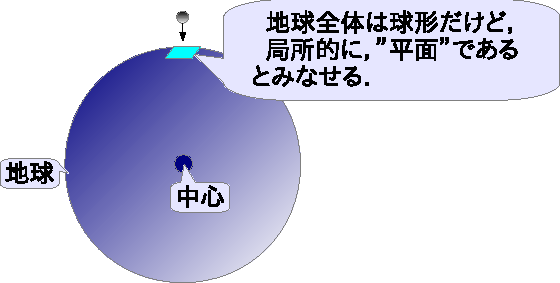
\includegraphics[keepaspectratio, width=6.5cm,height=4cm,clip]{ChiHyouHukin000.pdf}
                        \caption{地表付近は平面とみなしてよい}
                        \label{fig:HoubutsuSen}
                    \end{center}
                \end{figure}
            地球の重力加速度の方向は,常に物体から地球の中心へ向いている.
            地 とする.球表面付近では,重力加速度は鉛直下向きと近似できる
                \footnote{
                    「鉛直下向き」 とは,地表に垂直で,地表に向かう向きをいう.
                    鉛の球が重力で下向き(地球の中心に向かう向き)に引っ張られる
                    状況を描いたもの.物理学では,この表現がよく使われる.
                }.

            重力方向のみを考える場合,いちいち重力加速度をベクトル表記するのは
            面倒くさいし,読み手にしてみても式が煩雑で読みにくい.
            なので,重力加速度の向きが鉛直下向きであるという暗黙の了解をもたせて,
            方向の記述を省略することがほとんどである
                \footnote{
                    "省略" という言い方に躊躇するところがあるなら,
                    大きさのみに着目すると考えても同じことである.
                    要するに,重力加速度の定義の絶対値だけに着目して,
                    議論するということ.
                }.
            方向を省略すると,地球の重力加速度は
                \begin{equation*}
                    g = G\frac{M_{E}}{{r}^{2}}
                \end{equation*}
            となる.ここで,分母の ${|\br|}^{2}$ も,$r^{2}$ と略記した
                \footnote{
                    ベクトルを表す際の約束事として,ベクトル $\br$ の
                    大きさは,文字を細くして,$r$ と表す習慣がある.
                    細かいことを言うと,ベクトルの内積の公式のひとつに,
                    $\br\cdot\br = {\br}^{2} = |{\br}^{2}| = {|\br|}^{2} = r^{2}$
                    がある.
                }.

            さらに,ここで定義した地球の重力加速度に,地表からの高さ(いわば,標高)も
            組み込んで置きたい.方法は簡単で.地表からの高さを $h$ としたとき,
            $r$ に $r+h$ を代入してやればいい.
                \begin{align}
                    g = G\frac{M_{E}}{{(r+h)}^{2}}.
                \end{align}
            $r$ は地球の中心から地球表面までの距離である.
            地表からの高さを考慮したい場合は,地球の半径が大きくなったとして
            考えても同じ事で, $r$ に $h$ を加えるだけで済む.

            \begin{memo}{地表の重力加速度}
                地表なので,$h=0$として,計算しよう.
                地表の重力加速度 ${g}_{\mbox{地表}}$ は,
                \begin{align*}
                    {g}_{\mbox{地表}}
                    &= (6.673 \times 10^{-11}) \times
                        \frac{(5.974 \times 10^{24})}
                             {{(6.378 \times 10^{6})}^{2}} \\
                    %&= \frac{(6.673 \times 10^{-11}) \times (5.974 \times 10^{24})}
                    %         {{(6.378 \times 10^{6})}^{2}} \\
                    %&= \frac{39.864502 \times 10^{13}}{40.678884\times 10^{12}} \\
                    &= 9.799802275794 \\
                    &= 9.799  \,\mathrm{[m/s^{2}]} \quad \mbox{(有効桁数を考慮)}
                \end{align*}
                である.

                地球の重力加速度は大抵の場合,$g=9.80$[m/s] とされる.
                現実の地球は球形ではなく,楕円体である.だから,実際には地球の
                重力加速度は,場所ごとに違う.しかし,大まかな計算をする場合,
                $g=9.8$[m/s] として計算してよいだろう.

            \end{memo}

            \begin{memo}{エベレスト頂上の重力加速度}
                エベレスト頂上の標高は,8.848[km]であるという.
                なので,エベレスト頂上の重力加速度 ${g}_{\mbox{エベレスト頂上}}$ は,
                \begin{align*}
                    \mbox{}
                    &{g}_{\mbox{エベレスト頂上}} \\
                    &\quad = (6.673 \times 10^{-11}) \\
                    &\quad \quad \quad \times
                        \frac{(5.974 \times 10^{24})}
                             {{( (6.378 \times 10^{6}) + (8.848 \times 10^{3}) ) }^{2}} \\
                    %&= \frac{(6.673 \times 10^{-11}) \times (5.974 \times 10^{24})}
                    %         {{( (6.378 \times 10^{6}) + (8.848 \times 10^{3}) ) }^{2}} \\
                    %&= \frac{39.864502 \times 10^{13}}
                    %         {(40.678884 \times 10^{12})+(112.865088 \times 10^{9})+(78.287101 \times 10^{6})} \\
                    &\quad = 9.77266883...  \\
                    &\quad = 9.773 \,\mathrm{[m/s^{2}]} \quad \mbox{(有効桁数を考慮)}
                \end{align*}
                である.

                地表の重力加速度よりも小さい値となった.標高が $h=8.848$[km] の分,
                重力が弱まる.一般に,$h$ が大きいほど式の分母が大きくなり,重力が
                小さくなることは,容易にわかる.地球上で最大級の高さを誇る標高でも,
                $g=9.773$[m/s] で,$g=9.80$[m/s]と大差ない感じ
                    \footnote{
                        まあ,この差を大きいとみるか,小さいとみるかは,状況に
                        よるのだけど.
                    }.
            \end{memo}



%       %======================================================================
%       %  SubSection
%       %======================================================================
        \subsection{放物運動}
            \begin{mysmallsec}{概要}
            放物運動は,二次元的な(平面内の)運動である.つまり,2つの方向に対して
            運動方程式を考える必要がある.2方向として,垂直方向と水平方向を考える.
            ここで表現される水平とは,地上に対するものをいう.
            座標系は,垂直方向を $y$ とし,水平方向を $x$ とした直交座標とする.

            この2方向の運動は,互いに独立させて考えられる
                \footnote{
                    $x$ 方向の運動に,$y$ 方向の運動が影響することはない.逆も同じ.
                }.
            なので,垂直方向の運動と水平方向の運動を別々に考えた後,
            この2つの運動を重ねあわせることで放物物運動を見ていこう.
                \begin{figure}[hbt]
                    \begin{center}
                        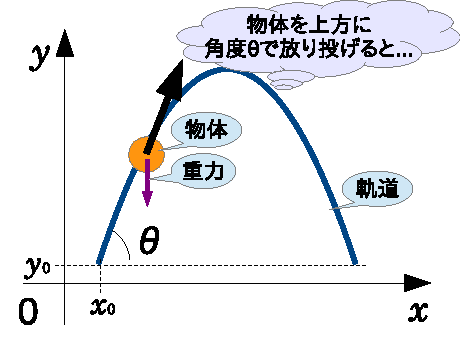
\includegraphics[keepaspectratio, width=6cm,height=6cm,clip]{HoubutsuSen.pdf}
                        \caption{放物運動}
                        \label{fig:HoubutsuSen}
                    \end{center}
                \end{figure}
            \end{mysmallsec}

            \begin{mysmallsec}{初期設定}
            初期設定を与えるところから,考察をはじめよう.
                \begin{itemize}
                    \item 開始時刻: $t=t_{0}$
                    \item 初期位置: ${\br}_{0} = \br(t_{0}) = (x(t_{0}),\, y(t_{0})) = (x_{0},\,y_{0})$
                    \item 初速度:  $\bv(t_{0})={\bv}_{0}$
                \end{itemize}
                        \begin{figure}[hbt]
                            \begin{center}
                                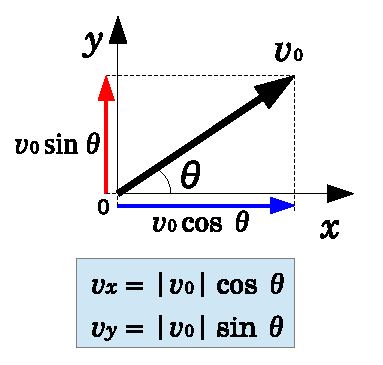
\includegraphics[keepaspectratio, width=6cm,height=6cm,clip]{HoubutsuSen_2.pdf}
                                \caption{放物運動開始}
                                \label{fig:HoubutsuSen}
                            \end{center}
                        \end{figure}

                初期条件から,垂直方向($y$ 軸方向)と水平方向($x$ 軸方向)の
                初速度$v_{x0},\,v_{y0}$ を求める.まず,図\ref{fig:HoubutsuSen}を
                みて,図形的イメージを覚えてもらいたい.やることは簡単で,
                三角関数を用いて,初速度 $\bv_{0}$ を $x$,$y$の各成分へ分解するだけだ.
                    \begin{align}
                        \mbox{(水平方向)} \quad v_{x0} &= |\bv_{0}| \cos \theta. \\
                        \mbox{(垂直方向)} \quad v_{y0} &= |\bv_{0}| \sin \theta.
                    \end{align}
            \end{mysmallsec}

            \begin{mysmallsec}{水平方向の運動方程式}
            水平方向の運動方程式の形は,
                \begin{equation*}
                    m\frac{{\df}^{2} x}{{\df t}^{2}} = F_{x}.
                \end{equation*}
            運動中は水平方向に力が働かないので,$F_{x} = 0$.よって,
                \begin{align}
                    m\frac{{\df}^{2} x}{{\df t}^{2}} = 0.
                \end{align}
            この方程式は,等速直線運動の方程式であり,以前に解いたことがある.
            速度は初速度のままで一定で,
                \begin{align}
                    v_{x}(t) = |\bv_{0}| \cos \theta
                \end{align}
            となる
                \footnote{
                    速度の関数に,独立変数として時間 $t$ を明示しているが,
                    左辺には時間は含まれいてない.これは時間に無関係であることを意味する.
                    しかし,ここではあえて,時間によらず一定であることを
                    示すために,時間を独立変数として記載することにしている.
                    理由は,垂直方向の速度は時間変化することと,対比したいからだ.
                }.
            位置は,
                \begin{align}
                    x(t) = v_{x}(t)t + x_{0} = (|\bv_{0}| \cos \theta)t +  x_{0}.
                \end{align}
            \end{mysmallsec}


            \begin{mysmallsec}{垂直方向の運動方程式}
                垂直方向の運動方程式は,
                    \begin{align}
                        m\frac{{\df}^{2} y}{{\df t}^{2}} = F_{y}.
                    \end{align}
                垂直方向は,重力が働いていることによる,等加速度運動である($F_{y}=-mg$)
                    \footnote{
                        1つ注意してほしい.重力加速度はベクトル量である.
                        だから,地球の重力加速度もベクトル表記して,$\bg$ と記述すべきだ.
                        だが,ここで考えているのは,垂直方向の1次元なので,ベクトル表記は
                        していない.
                    }.
                重力を運動方程式に代入し,整理しよう.
                    \begin{align*}
                        m\frac{{\df}^{2} y}{{\df t}^{2}} &= -mg \\
                         \frac{{\df}^{2} y}{{\df t}^{2}} &= -g. \quad(m \mbox{で両辺を割った})
                    \end{align*}
                等加速度運動についても,前に計算してあるので,ここではその結果を使う.
                加速度が $g$ の場合,等加速度運動の速度は,
                    \begin{equation*}
                        v_{y}(t) = -gt + v_{y0} = -gt + |\bv_{0}| \sin \theta.
                    \end{equation*}
                位置は,
                    \begin{equation*}
                        y(t) = -\frac{1}{2}g{t}^{2} + v_{y0}t + y_{0} = -\frac{1}{2}g{t}^{2} + (|\bv_{0}| \sin \theta)t + y_{0}.
                    \end{equation*}
            \end{mysmallsec}


            \begin{mysmallsec}{まとめ}
                以上の結果をまとめておこう.
                放物運動する物体の位置と速度は,
                \begin{align}
                                         \begin{bmatrix}
                                         x(t)   \\
                                         y(t)
                                 \end{bmatrix}
                            &=    \begin{bmatrix}
                                     (|\bv_{0}| \cos \theta)t +  x_{0}  \\
                                    -\frac{1}{2}g{t}^{2} + (|\bv_{0}| \sin \theta)t + y_{0}
                                 \end{bmatrix}.
                                 \\ \notag \\
                                                 \begin{bmatrix}
                                         v_{x}(t)  \\
                                         v_{y}(t)
                                 \end{bmatrix}
                            &=    \begin{bmatrix}
                                         |\bv_{0}| \cos \theta \\
                                         -gt + |\bv_{0}| \sin \theta
                                 \end{bmatrix}.
                \end{align}
            \end{mysmallsec}



%       %======================================================================
%       %  SubSection
%       %======================================================================
        \subsection{宇宙速度}
            宇宙空間で運動するために必要な速度のことを,
            \textbf{宇宙速度} という.
            宇宙速度とは,慣性運動のみで宇宙空間へ到達するために,
            最初に与える最低初速度をいう
                \footnote{
                    宇宙速度は,
                    宇宙空間に飛びたすために,絶対に書かせいない
                    速度ではない.地球の重力以上の力を対象物に与え続けられるのであれば,
                    どんなに遅くとも,宇宙空間に到達させることができる.
                    宇宙速度という概念は,慣性によって,宇宙へ到達するための初速度である.
                }.
            宇宙速度には3つの段階があって,
            それぞれ,\textbf{第一宇宙速度},\textbf{第二宇宙速度},
            \textbf{第三宇宙速度} とよばれる.
            各宇宙速度は,下のように定義される.
            \begin{description}
                \item[第一宇宙速度]\mbox{}\\
                    地表ギリギリで,等速円運動を続けるために必要な最小初速度.
                    地球と同じ大きさ,同じ質量の球体を地球に見立てて計算される値.
                    なので,空気抵抗や,建築物の有無は考慮しない.
                    地球の人工衛星になりたい場合に,必要な速度.
                \item[第二宇宙速度]\mbox{}\\
                    地球の重力を振り切り,地球圏外へ脱出するために必要な最小速度.
                    \textbf{脱出速度} といわれることも多い.
                    太陽の人工惑星になりたい場合に,必要な速度.
                \item[第三宇宙速度]\mbox{}\\
                    太陽圏外に脱出するために必要な最小速度.
                    太陽系にいるのが嫌になったときに,太陽系から脱出するために
                    は少なくともこの速度をもっていなければならない.
            \end{description}

        \subsubsection{第一宇宙速度}
            第一宇宙速度,要するに,地球の人工衛星になるために最低必要な速度,を計算しよう.
            何より最初に,運動方程式をたてよう.人工衛星になるためには,
            地球の周りを等速円運動しないといけない.人工衛星にしたい物体の速度を $v$ としたとき,
            半径 $R_{E}$ の地球の表面に軌道を描くには,万有引力と向心力を用いて,以下の方程式を
            満たす必要がある.向心力と万有引力は次の通り.
            \begin{align*}
                \mbox{(向心力)}   &= \frac{mv^{2}}{R_{E}+h}. \\
                \mbox{(万有引力)} &= G\frac{mM_{E}}{(R_{E}+h)^{2}}.
            \end{align*}
            よって,満たすべき方程式は,
            \begin{align}
                \frac{mv^{2}}{R_{E}+h} = G\frac{mM_{E}}{(R_{E}+h)^{2}}.
            \end{align}

            式を整理して,$v$ について解こう.
            \begin{align*}
                \frac{mv^{2}}{R_{E}+h} &= G\frac{mM_{E}}{(R_{E}+h)^{2}} \\
                v^{2} &= G\frac{M_{E}}{R_{E}+h}
            \end{align*}
            以上から,
            \begin{align}
                v = \sqrt{G\frac{M_{E}}{R_{E}+h}}. \quad (v<0\mbox{の解は除外})
            \end{align}

            $h=0$(地表すれすれを想定)のとき,上記の値 $G$,$M_{E}$,$R_{E}$ を
            代入してみよう.計算すると,
            \begin{align*}
                v &= \sqrt{(6.67 \times 10^{-11}) \times \frac{(5.97 \times 10^{24})}{(6.37 \times 10^{6})+0}} \\
                  &= \sqrt{\frac{6.67 \times 5.97}{6.37} \times  \frac{10^{-11} \times 10^{24}}{10^6{}}} \\
                  &= \sqrt{\frac{6.67 \times 5.97}{6.37} \times  10^{7}} \\
                  &= 7906.42 ...... \\
                  &= 7.91 \times 10^{3} \,\mathrm{[m/s]} \mbox{(有効桁数を考慮)}
            \end{align*}
            となった
                \footnote{
                    Python(2.7.3)を使って計算した.\sf{import math} で数学関数をインポートした後,
                    \sf{math.sqrt((6.67*5.97/6.37)*10**7)} を実行し,出力\sf{7906.428836995505} を得た.
                }.

            以上から,第一宇宙速度は,$7.91 \times 10^{3}$ [m/s] であることがわかった.


        \subsubsection{第二宇宙速度}
            第二宇宙速度は,地球の重力圏外に脱出するのに,最低限必要な初速度である.
            つまり,重力から生じる位置エネルギーを振り払うだけの速度(運動エネルギー)を
            与えてやらないといけない.言い換えると,
            運動エネルギーと地球の位置エネルギーの和が0以上
            になるように,初速度を与えるということだ
                \footnote{
                    重力による位置エネルギーは負であるから,合計が正になるような運動エネルギー
                    が必要とされる.
                }.

            地球の重力の位置エネルギー $U_{E}$ は
                \begin{equation*}
                    U_{E}=-G\frac{mM_{E}}{R_{E}+h}
                \end{equation*}
            である.ここで,上式は,地表から $h$ だけ上方の位置エネルギーを表している.
            よって,この位置エネルギー以上の運動エネルギーを与えればよい.
                \begin{equation*}
                    \frac{1}{2}mv^{2} + U_{E} \geq 0,
                \end{equation*}
            すなわち,
                \begin{align}
                    \frac{1}{2}mv^{2} - G\frac{mM_{E}}{R_{E}+h} \geq 0
                \end{align}
            を満たす $v$ であればよい.

            $v$ について解くと,
                \begin{align*}
                    \frac{1}{2}mv^{2} - G\frac{mM_{E}}{R_{E}+h} &\geq 0 \\
                    \frac{1}{2}v^{2}  - G\frac{M_{E}}{R_{E}+h}  &\geq 0 \\
                    \frac{1}{2}v^{2}                        &\geq  G\frac{M_{E}}{R_{E}+h} \\
                               v^{2}                        &\geq 2G\frac{M_{E}}{R_{E}+h} \\
                               v                            &\geq \sqrt{2G\frac{M_{E}}{R_{E}+h}}.
                \end{align*}
            最後の変形で,$v<0$ を除外した.第二宇宙速度は上式を満たす最小の $v$ であることから,
                \begin{align}
                    v = \sqrt{2G\frac{M_{E}}{R_{E}+h}}.
                \end{align}
            で計算できる.

            これに具体的な数値を代入してみよう($h=0$ として,地表すれすれを想定).すると,
                \begin{align*}
                    v &= \sqrt{2 \times (6.67 \times 10^{-11}) \times \frac{5.97 \times 10^{24}}{6.37 \times 10^{6}+0}} \\
                      &= \sqrt{\frac{2 \times 6.67 \times 5.97}{6.37} \times \frac{10^{-11} \times 10^{24}}{10^{6}}}    \\
                      &= \sqrt{\frac{2 \times 6.67 \times 5.97}{6.37} \times 10^{7}}   \\
                      &= 11181.37  ...... \\
                      &= 11.2 \times 10^{3} \,\mathrm{[m/s]}\mbox{(有効桁数を考慮)}
                \end{align*}
            となった
                \footnote{
                    Python(2.7.3)を使って計算した.\sf{import math} で数学関数をインポートした後,
                    \sf{math.sqrt((2*6.67*5.97/6.37)*10**7)} を実行し,出力\sf{11181.378891216778} を得た.
                }.

            以上から,第二宇宙速度は,$11.2 \times 10^{3}$ [m/s] であることがわかった.

            \begin{memo}{補足}
                第一宇宙速度と第二宇宙速度には,簡単な数値関係が知られている.というのも,
                    \begin{equation*}
                        \mbox{"第二宇宙速度"} = \sqrt{2}\mbox{"第一宇宙速度"}
                    \end{equation*}
                という関係があるのだ.実際に,
                \begin{align*}
                    \mbox{"第一宇宙速度"} \quad \sqrt{G\frac{M_{E}}{R_{E}+h}}  \\
                    \mbox{"第二宇宙速度"} \quad \sqrt{2G\frac{M_{E}}{R_{E}+h}}
                \end{align*}
                であり,
                    \begin{equation*}
                        \sqrt{2G\frac{M_{E}}{R_{E}+h}} = \sqrt{2} \sqrt{G\frac{M_{E}}{R_{E}+h}}
                    \end{equation*}
                が成立している.

                この規則を知っていると,第一宇宙速度と第二宇宙速度のどちらか一方が計算済みなら,
                他方を計算するのが楽になる.単に,$\sqrt{2}$ 倍,あるいは,$1/\sqrt{2}$ 倍すれば
                いいのだ.
            \end{memo}


        \subsubsection{第三宇宙速度}
            計算中.


    \subsection{躍度(jerk)と運動方程式}
        躍度$\bj$の定義式は以下であった\footnote{\ref{seq:jerk_define}節の式\eqref{eq:jerk_define}を参照.}.
        \begin{align*}
            \bj &:= \frac{\df \ba}{\df t} = \frac{{\df}^{3} \bx}{{\df t}^{3}}.
        \end{align*}

        これと運動方程式を関連づけてみよう.
        運動方程式は
            \[
                m\frac{{\df}^{2} \bx}{{\df t}^{2}} = \bF.
            \]
        であった.この式の両辺を時間微分すると,左辺に$\bj$が現れる.
        \begin{align*}
            m\frac{{\df}^{3} \bx}{{\df t}^{3}} &= \frac{\df \bF}{\df t}. \\
            \therefore \quad m\bj &= \frac{\df \bF}{\df t}.
        \end{align*}
        この式から,力の時間変化によって躍度(jerk)を発生させると解釈してよいだろう.

        人が物体を手で引っ張っている状況を想像してみると,常に正確に一定の力で引っ張ることは
        不可能である.機械に頼ったとしても,ブレはあるはず.
        それに,摩擦があることも想定できて,この場合は凸凹加減に場所によって物体にかかる合力
        が変わってくる.

        乗り物(車/電車/飛行機など)に乗っているとき,躍度が生じると不快感を感じる.
        車の停止状態からアクセルを踏む強さを急激に変えると,
        加速度が$\bzero$の状態から急に大きくなるため大きな躍度が生まれる.
        また,減速時もおなじである.等速直線運動していたとして,急にブレーキを踏めば,
        進行方向と逆向きの大きな加速度が生じる.

        躍度は実際には毎日ごく当たり前に感じている間隔を説明する大事な概念である.
        だけど,力学の教科書には躍度の紹介がないのはなぜだろうか.




    \subsection{円錐振り子}
    \begin{figure}[hbt]
        \begin{center}
            \includegraphicsdefault{ensui_furiko.pdf}
            \caption{円錐振り子}
            \label{fig:ensui_furiko}
        \end{center}
    \end{figure}

    \subsection{調和振動(単振動)}
    \subsubsection{弾性力}
        物体に対して,破壊しない程度の力を与えて,物体に歪を与えると,もとの形に戻ろうとする力が生じる.
        この力を \textbf{弾性力} という.

    \subsubsection{フックの法則}
        バネになんの力も加えられていない場合,その自然の長さを${l}_{0}$とする.
        バネの一端を固定し,他方を指でつまんで長さ$l$となるように力$\bF$で引っ張ってみる.
        このとき,バネからは縮もうとする向きに力が働く.このバネの力を$\bS$で表そう.
        $\bS$は弾性力の一種である.もとに戻ろうとする力というイメージから,\textbf{復元力} と
        もよばれる.
        バネを伸ばす力$\bF$と復元力$\bS$は互いに作用反作用の関係にある.よって,
        \begin{align}
            \bS = -\bF
        \end{align}
        の関係にある.

        \begin{figure}[hbt]
            \begin{center}
                \includegraphicsdefault{hookes_law.pdf}
                \caption{フックの法則}
                \label{fig:hookes_law}
            \end{center}
        \end{figure}
        バネの種類によって,その復元の力の置きさはことなる.
        その指標を \textbf{バネ定数} と名付けて,$k$とかくことにする.
        復元力の大きさは,バネの自然の長さからの変位$l-{l}_{0}$に比例することが知られていて,
        バネ定数$k$はこの比例定数である.式にすると,
        \begin{align}
            S = -k(l-{l}_{0})
        \end{align}
        である.ただし,バネが伸びる方を正の向きとする.バネが伸びるとき$S$は正の値をとり,
        バネが縮んでいるときは,$S$は負の値となる.自然の長さのとき,つまり,$l={l}_{0}$の
        場合は$S=0$であり,復元力は生じない.しかし,慣性の法則により,$S=0$のときにも運動
        は止まることはない.止まらなかった結果,バネが伸びる(あるいは縮む)ので,復元力が
        再び生じて延々と運動を繰り返す.

        バネの長さ$l$が自然長の長さ${l}_{0}$より長いとき(バネを引っ張っているとき)は
        \begin{align*}
                                      l  &> {l}_{0} \\
            \Leftrightarrow l - {l}_{0}  &> 0       \\
            \therefore S = -k(l-{l}_{0}) &< 0
        \end{align*}
        となり,$S$が負になるので,バネを引っ張る場合は縮む向きに復元力が働くことが式で
        表現できている.バネの長さ$l$が自然長の長さ${l}_{0}$より短いとき(バネを縮めているとき)は
        \begin{align*}
                                      l  &< {l}_{0} \\
            \Leftrightarrow l - {l}_{0}  &< 0       \\
            \therefore S = -k(l-{l}_{0}) &> 0
        \end{align*}
        となり,$S$が正になっていて,バネが伸びる向きに復元力が生じる.


    \subsubsection{単振動の種類}
        バネにくっついた物体が上下あるいは左右などに揺れている様子を \textbf{単振動} という.
        上下/左右ではなくても一方向の定常的な揺れであれば単振動である.摩擦などがあって徐々に振動が
        弱くなっていく場合は \textbf{減衰振動} という.物体がついていないもう片方の端っこ部分を
        振動させた場合は,\textbf{強制振動} という.教科書でよく例題として取り上げられるのは
        これくらいかな.
        \begin{figure}[hbt]
            \begin{center}
                \includegraphicsdefault{tanshindo_0.pdf}
                \caption{調和振動(単振動)}
                \label{fig:tanshindo_0}
            \end{center}
        \end{figure}


    \subsubsection{調和振動の運動解析}
    \begin{mysmallsec}{例題設定}
        バネ定数$k$のバネににつながった物体の動きを物理的に解析する.
        物体にかかる力は,重力$m\bg$とそれに対応する床からの垂直抗力$\bN$,バネから受ける弾性力$\bF$の3つである.
        今から考える状況はバネは水平にして,重力に対して垂直に運動するような場合を想定する.
        外力を与えない,バネのみの力による運動とする.図\ref{fig:tanshindo_1}にそのイメージを描く.
        図の上部が伸びが最大,図の下部が伸びが最小,それらの中間がバネが自然な長さにある瞬間を描いた.
        \begin{figure}[hbt]
            \begin{center}
                \includegraphicsdefault{tanshindo_1.pdf}
                \caption{調和振動の運動解析}
                \label{fig:tanshindo_1}
            \end{center}
        \end{figure}
    \end{mysmallsec}

    \begin{mysmallsec}{座標の設定}
        真横に振動する1次元の調和振動についての現象を解析するということだ.
        3次元座標のうち,$y$座標と$z$座標は常に0であるように座標を張ると,運動方程式が簡単になるので
            \footnote{
                教科書のような理想的な状況設定だと,調和振動は一方向のみの振動なので,
                全方向に成分を持つように座標を張ることは,座標設定ミスである.
                座標は計算しやすいように考えてから設定すべきだ.
            },
        物体の位置$\br$は次のように設定する.
        \begin{align}
            \br(t) = (x(t), \, y(t), \, z(t)) \left[= (x(t),\,0,\,0)\right].
        \end{align}
        ここで,カッコ$\left[\right]$でくくった部分$(x(t),\,0,\,0)$は次の初期値によって
        計算される結果であり,仮定ではない.逆に以下で,このようになるように,初期値を設定する.
    \end{mysmallsec}

    \begin{mysmallsec}{初期値}
        \begin{itemize}
            \item バネが自然の長さにあるときの物体の位置を${x}_{n}$とする

            \item $t=0$のときの物体の位置$\br(0)$を以下のようにとる
                  \begin{align}
                      \br(0) = (x(0), \, y(0), \, z(0)) := (x(0),\,0,\,0).
                  \end{align}
            \item 初速度$\bv(0)$はどの方向にも与えず,どの方向も0であるとする
                  \begin{align}
                      \bv(0) = ({v}_{x}(0), \, {v}_{y}(0), \, {v}_{z}(0)) := (0,\,0,\,0).
                  \end{align}
            \item 摩擦はなく,空気抵抗もなく,重力は至るところで均一で,外力も全く加えず,
                  電場や磁場もないし,当然,素粒子レベルの強い力や弱い力なんかは想定の範囲外
        \end{itemize}
    \end{mysmallsec}

    \begin{mysmallsec}{方向成分の解析(1):$y$成分と$z$成分}
        まず簡単な,$y$軸方向と$z$軸方向の運動を解析する.ここで設定した状況は,
        $y$方向へも$z$方向へも運動しない(位置を変えない)ように初期値設定と座標設定をしたはずである.
        そのことを確認しよう.

        バネから受ける弾性力$\bF$を成分表示すると,
            \begin{align}
                \bF = ({F}_{x}, \, {F}_{y}, \, {F}_{z}) = ({F}_{x},\,0,\,0).
            \end{align}
        となる.3次元ベクトルのまま考えてもよいが,この場合,$y$方向と$z$方向については位置の変化はない.
        例えば,$y$方向の位置と速度は,時間を独立変数として,位置を$y(t)$,速度を${v}_{y}(t)$とすると
        次のように計算される.
            \begin{align*}
                                m\frac{{\df}^{2} y(t)}{{\df t}^{2}}      &= {F}_{y}     \\
                \Leftrightarrow m\frac{{\df}^{2} y(t)}{{\df t}^{2}}      &= 0           \\
                \Leftrightarrow  \frac{\df}{\df t}\frac{\df y(t)}{\df t} &= 0           \\
                \therefore       \frac{\df y(t)}{\df t}                  &= {v}_{y}(0). \\
                \therefore      y(t)                                     &= {v}_{y}(0)t + y(0).
            \end{align*}
        初期値${v}_{y}(0):=0$,$y(0):=0$だから,
        \begin{align}
            y(t) = 0.
        \end{align}
        よって,$y$方向には微動だにしない.

        $z$軸方向も$y$軸方向と同じ条件なので,
        \begin{align}
            z(t) = 0.
        \end{align}
        である.
    \end{mysmallsec}

    \begin{mysmallsec}{方向成分の解析:(2)$x$成分}
        $x$軸方向にはバネの伸び縮みによる復元力が生じているので,
        フックの法則が使える.$x$方向に働く力${F}_{x}$は,バネ定数を$k$,
        バネの自然の長さを${x}_{n}$としたとき,
        \begin{align}
            {F}_{x} = -k(x(t)-{x}_{n})
        \end{align}
        で与えられる.よって,運動方程式は
        \begin{align}
            m\frac{{\df}^{2} x(t)}{{\df t}^{2}} = -k(x(t)-{x}_{n})
        \end{align}
        である.ここで,
        \begin{align}
            X(t) :=  x(t) - {x}_{0}
        \end{align}
        とおくと,
        \[
            \frac{\df X(t)}{\df t} = \frac{\df x(t)}{\df t} \, , \quad \frac{{\df}^{2} X(t)}{{\df t}^{2}} = \frac{{\df}^{2} x(t)}{{\df t}^{2}}
        \]
        であるから,
        \begin{align}
                            m\frac{{\df}^{2} X(t)}{{\df t}^{2}} &= -kX(t) \notag \\
            \Leftrightarrow \frac{{\df}^{2} X(t)}{{\df t}^{2}}  &= -\frac{k}{m}X(t)
        \end{align}
        となる.微分方程式を解くと,
        \begin{align}
                             X(t)            &= A \sin \sqrt{\frac{k}{m}} t + B \cos \sqrt{\frac{k}{m}} t \notag \\
            \Leftrightarrow  x(t) - {x}_{0}  &= A \sin \sqrt{\frac{k}{m}} t + B \cos \sqrt{\frac{k}{m}} t \notag \\
            \therefore       x(t)            &= A \sin \sqrt{\frac{k}{m}} t + B \cos \sqrt{\frac{k}{m}} t + {x}_{0}
        \end{align}
        を得る.角周波数$\sqrt{k/m}$を$\omega$でとおいてやると,見やすくなる.
        \begin{align}
            \omega := \sqrt{\frac{k}{m}}.
        \end{align}
        \begin{align}
            x(t) &= A \sin \omega t + B \cos \omega t + {x}_{0}.
        \end{align}

    \end{mysmallsec}

    \begin{mysmallsec}{結果}
        一次元の調和振動の解析結果.
        \begin{align}
            \br(t) &= (x(t),\,y(t),\,z(t)) \notag \\
                   &= (x(t),\,0,0)  \notag \\
                   &= (A \sin \omega t + B \cos \omega t + {x}_{0},\,0,\,0)
        \end{align}
    \end{mysmallsec}



\chapter{惑星の運動}
%   %-----------------------------------------------------------------------------------------------
%   %  Input
%   %    File Name : PhysNote_CM_Kepler.tex
%   %    説明      : ニュートンの法則から,ケプラーの法則を導く
%   %-----------------------------------------------------------------------------------------------
        %   %==========================================================================
%   %  Section
%   %==========================================================================
    \section{はじめに}
        ニュートンはデカルトやガリレイらの先人の考えに影響を受けながら,
        力学を構築した.この先人の中にはケプラー
            \footnote{
                Johannes Kepler ( 1571 - 1630,ドイツ )
            }
        の名前もあり,万有引力の法則は,
        ケプラーの法則を説明するために考え出されている.
        と言っても,万有引力の法則は,惑星だけの性質ではなく,
        世の中に存在する全ての物体が持つべき性質であると,理解が拡張されている.
        ニュートンは,惑星の運動と地上の物体の運動は同じ運動法則に従っている,
        と主張するのである.

        惑星の軌道に関する情報は,ケプラーよりも前の時代に,ティコ$\cdot$ブラーエ
            \footnote{
                Tycho Brahe ( 1546 - 1601,デンマーク )
            }
        が膨大な観測データを残していた.ケプラーは,このデータに規則性を見出し,
        惑星の運動に関する3つの法則を見つけ出した.今日では \textbf{ケプラーの法則} と呼ばれる,
        さらにその後,ニュートンはケプラーの3つの法則を包括するような,力学体系を
        築いた.これが現在のニュートン力学と呼ばれるものである.地上の物体
        の運動と,惑星の運動は同じ法則に従っていることを示したのである.

        惑星の運動の記述は,このように,ニュートン力学の1つのクライマックスでもある.
        惑星の運動が分からずに,ニュートン力学を学んだとは言えない.

        この章では惑星の運動の記述を考えていこう.

%   %==========================================================================
%   %  Section
%   %==========================================================================
    \section{ケプラーの法則}
            ケプラーはティコ$\cdot$ブラーエの残した,膨大な惑星の観測データから,
            惑星の運動軌道は,次の3つの法則によって,説明できることを
            発見した.
            \begin{myshadebox}{ケプラーの法則(惑星の運動に関する3つの法則)}
                惑星の運動は,以下の3つの法則に従っている.
                \begin{description}
                    \item[第1法則(楕円軌道の法則)]\mbox{}\\
                      惑星は太陽を1つの焦点とする,楕円軌道を描く.
                    \item[第2法則(面積速度一定の法則)]\mbox{}\\
                      一定時間に, 太陽と惑星を結ぶ動径が掃く面積は一定である.
                    \item[第3法則(調和の法則)]\mbox{}\\
                      惑星の公転周期の2乗と, 惑星の太陽からの距離の3乗の比は,どの惑星でも一定である.
                \end{description}
            \end{myshadebox}

            まずこれらを数式で表現してみよう.

%       %======================================================================
%       %  SubSection
%       %======================================================================
        \subsection{楕円の方程式}
            楕円を数式で表そう.
            \begin{figure}[hbt]
                \begin{center}
                    \includegraphicsdefault{daen_kepler.pdf}
                    \caption{楕円と座標・方程式}
                    \label{fig:daen_kepler}
                \end{center}
            \end{figure}


%       %======================================================================
%       %  SubSection
%       %======================================================================
        \subsection{極座標での運動方程式}
            惑星の運動は角運動であるから,極座標を採用する.
            水平方向の角度を $\phi$,高さ方向の角度を $\theta$,原点からの
            直線距離を $r$ とする.点Pは ($r$,\,$\theta$,\,$\phi$) と表現される.

%       %======================================================================
%       %  SubSection
%       %======================================================================
        \subsection{第1法則;楕円軌道の法則}
        \begin{figure}[hbt]
            \begin{center}
                \includegraphicsdefault{wakusei_kepler_low.pdf}
                \caption{惑星の楕円軌道}
                \label{fig:wakusei_kepler_low}
            \end{center}
        \end{figure}

%       %======================================================================
%       %  SubSection
%       %======================================================================
        \subsection{第2法則;面積速度一定の法則}
        \begin{figure}[hbt]
            \begin{center}
                \includegraphicsdefault{wakusei_kepler_low2_menseki.pdf}
                \caption{面積速度一定}
                \label{fig:wakusei_kepler_low}
            \end{center}
        \end{figure}

%       %======================================================================
%       %  SubSection
%       %======================================================================
        \subsection{第3法則;調和の法則}


\chapter{解析力学}
%   %-----------------------------------------------------------------------------------------------
%   %  Input
%   %    File Name : PhysNote_CM_Analysis.tex
%   %    説明      : ニュートン力学を数学的に扱いやすくし,一般化する
%   %-----------------------------------------------------------------------------------------------
        %   %==========================================================================
%   %  Section
%   %==========================================================================
    \section{はじめに}
%       %======================================================================
%       %  SubSection
%       %======================================================================
        \subsection{教科書}
            使用する教科書は,下記の通り.
            \begin{itemize}
                \item
                    早田 次郎 [著],
                    『現代物理のための 解析力学』,
                     サイエンス社
                 \item
                    小出 昭一郎 [著],
                    『物理入門コース 解析力学』,
                    岩波書店
            \end{itemize}

%       %======================================================================
%       %  SubSection
%       %======================================================================
        \subsection{解析力学とは}
            解析力学とは,ニュートン力学を数学的に一般化し,整理しなおしたもの
            である.要は,力学を数学的に扱うのである.そうすることで,そのままの
            ニュートンの運動方程式では解きにくかった問題を,容易に解けるようになる.
            また,とても不思議なことだが,量子力学の定式化をはじめとし,
            現代の物理学では解析力学がその土台となっている.
            言い換えると,現代の物理学で表現される数式は,解析力学で示される
            方程式に則って表現されるのである.

            ただ,表現が数学的であるため,物理的意味をイメージする
            ことは難しい.なので,解析力学を学ぶにあたって,その物理的意味を
            考えないようにしたい.解析力学を学ぶ理由は,現代物理学の土台を
            学ぶことであり,物理学の体系的な理解をすることであり,力学的な問題の
            解決をいくらか容易にすることである.ニュートンが運動の法則を数式で
            表現してくれたのだから,これを数学的に解析し,計算しやすく一般化
            しないのではもったいない.

            だから,これからしばらくは,物理的イメージがどうのこうのというよりも,
            ニュートンの運動方程式を数学的にどのように解くかに注目していきたい.
            物理を離れて,数学を学習している気分になってしまうかもしれないが,
            これは仕方ないだろう.

            解析力学とは,物理学的な問題をとくための数学的な手法であり,
            現代物理学の目標の1つである,統一理論
                \footnote{
                    物理学の目的は,世界に存在する物質が従う,最も根源的な法則の発見である.
                    その目的の達成似必要な情報の1つに,重力,電磁気力,弱い相互作用,強い相互作用の,4つの
                    力を一気に説明するような,1つの方程式をみつけることがある.
                    そのような理論を,(力の)統一理論とよんでいる.正確には,
                    超大統一理論といわれるのだが,細かいことは気にしない.
                    簡単な概念については,そのへんの啓蒙書をあさってみるとよい.
                }
            を見つけ出すための基礎である.解析力学なしに,現在の物理学は
            成り立たない.

%       %======================================================================
%       %  SubSection
%       %======================================================================
        \subsection{解析力学の目的}
            解析力学の学習目的は,ニュートン力学では解くのに難しかった問題
                \footnote{
                    例えば,2つのおもりが直列につながっている振り子とか.
                }
            を,数学的手法を駆使することで,比較的簡単に解けるようになること
            である.これが,最初に解析力学を学習する最も一般的な目標だろう.
            しかし,解析力学の学習は,上にも書いたように,別のもっと重要な
            目的がある.それは,物理学の各分野の統合に使われるということに,
            注目される.物理学を統一的に扱うには,より一般的に通用する
                \footnote{
                    一般的といったのは,ニュートン力学や電磁気学,熱力学,
                    相対性理論,量子力学といった分野にまたがるという
          +          意味で使った.解析力学的表現は,不思議なことに,
                    すべての物理学を統一的に表現するのに都合が良いみたいだ.
                }
            ことが必要である.物理学の各分野を統一するような,数学的表現
            方法が欲しいのである.そして,解析力学は,その要求を満たす.

            解析力学は,ニュートンの運動方程式のままでは解くのに難しい問題を
            簡単化することができ,さらに加えて,現代の物理学の最も基本的な
            考え方となっている.

            とはいうものの,解析力学は数学ではなく,物理学である.だけども,
            物理学を数学っぽく扱うので,物理っぽくない.おそらく,
            初学者は,解析力学のどっちつかずの性格に戸惑うはず.しかし,
            ここは割り切って,「超便利ツールの習得」と考えて,
            解析力学を学んでほしい.少々数学的に無理な仮定や考え方を含んでいたり,
            物理的に考えて意味のわからない概念の導入があるが,気にしない.
            とにかく学習してみよう.学習を終えたら,あるいはその途中で,
            解析力学の凄さ,恐ろしさを感じるだろう.


%   %==========================================================================
%   %  Section
%   %==========================================================================
    \section{速習:解析力学}\label{sec:sokushu_kaisekirikigaku}
        \begin{mycomment}
            解析力学のその核心は,いかにも数学的で,いきなりその理論に
            挑んでも,おそらく挫折してしまうだろう.挫折しないのは,
            数学がとても好きな人か,直ぐに鵜呑みにする人か,もしくは,
            ご聡明なお方だけであり,たいていの人は混乱し,諦めがちだ.

            なので,はじめに,解析力学とはどのようなものであるかを,
            今までの知識からわかるように,変分原理を用いずに解析力学の
            主要方程式を導く.この過程で,解析力学で扱う方程式について,
            おおよそのイメージをつかんでもらいたい.

            もちろん,変分原理の理論も大事なので,そのあとで改めて,解説する.
        \end{mycomment}
%       %======================================================================
%       %  SubSection
%       %======================================================================
        \subsection{時間微分の省略記号}
            時間に関する微分,つまり時間微分の記号の省略記号を導入しよう.
            これから,時間微分を多用するからである.もちろん今までの
            時間微分の記号 $\df/\df t$ も使用する.式表現が複雑になる場合に
                \footnote{
                    または,単に記述が面倒な場合でも.
                },
            省略記号を使う.

            省略記号は,次のようなものである.
                \begin{align}
                    \dot{\br} := \frac{\df r}{\df t}.
                \end{align}
            時間微分の対象となる関数の上にドット記号「$\dot{\mbox{}}$」を
            つけるだけである.

            この例の場合,時間微分したいのは位置 $\br := \br(t)$ である.
            位置を時間微分したものが速度なので,速度を $\bv(t)$ とすれば,
                \begin{equation*}
                    \bv = \dot{\br} := \frac{\df r}{\df t}.
                \end{equation*}
            である.

            更に,2階微分をしたい場合には,ドットを2つ付ける($\ddot{\br}$).
                \begin{equation*}
                    \ba = \dot{\bv} = \ddot{\br} = \frac{{\df}^{2} r}{{\df t}^{2}}.
                \end{equation*}

            同様に,3階以上の微分でもその分だけドット「$\dot{\mbox{}}$」をつ
            ればいい.ただし,見難くなるし,あまり使われない.

            このように,時間微分を植え付きのドットで表す記法を,
            \textbf{ニュートン記法} と呼んだりする.ちなみに,
            今までの微分記号 $\df/\df t$ は \textbf{ライプニッツ記法} と
            いう.

            以降では,ニュートン記法とライプニッツ記法を混合して使うが,
            その使い分けに特別な規則はない.単に,式を綺麗に書きたいという
            だけである.あまり気にしないで欲しい.

%       %======================================================================
%       %  SubSection
%       %======================================================================
        \subsection{ラグランジュ形式の解析力学}
            \begin{mycomment}
                ニュートンの運動方程式をいじくって,数学的に扱いやすくする.
                その結果として得られる方程式は \textbf{ラグランジュ
                    \footnote{www
                    }
                の運動方程式} とよばれる.これから,ラグランジュの運動方程式を,
                簡略的に,導出してみよう.

                話が長くなるので,段階を追って節を区切る.
            \end{mycomment}

%           %==================================================================
%           %  SubsubSection
%           %==================================================================
            \subsubsection{ニュートン方程式の復習}
            まずはニュートンの運動方程式がないと話が始まらない.
            物体の運動方程式は,次のようであった.
                \begin{align}
                    \bF = m\ddot{\br} = m \frac{{\df}^{2} \br}{{\df t}^{2}}.
                \end{align}
            ここに,$m$ は物体の質量,$\br$ は物体の位置,$\bF$ は
            物体の受ける力であり,$t$ はもちろん時間を表す.

%           %==================================================================
%           %  SubsubSection
%           %==================================================================
            \subsubsection{力とポテンシャル$\cdot$エネルギーの関係式}
            ニュートン力学によると,力はポテンシャル$\cdot$エネルギー
            の勾配と考えられる.そしてそれは,位置 $\br$ で偏微分
            することである.すなわち,
                \begin{align}
                    \bF = \dgrad U = -\frac{\rd U}{\rd \br}.
                \end{align}
            この場合,
            力は \textbf{保存力} であるという条件がつく.
            以降では,力は保存力であるとして,話を進めよう.

            力とポテンシャル$\cdot$エネルギーの関係式,すなわち,
                \begin{equation*}
                    \bF = -\frac{\rd U}{\rd \br}
                \end{equation*}
            を,ニュートンの運動方程式の左辺に考慮すると,
                \begin{align}
                    -\frac{\rd U}{\rd \br} = m\ddot{\br} = m \frac{{\df}^{2} \br}{{\df t}^{2}}.
                \end{align}

            次に,右辺 $m\ddot{\br}$ に注目しよう.
            運動量 $\bp := m\bv = m\dot{\br}$ を
            導入すると,
                \begin{align}
                    -\frac{\rd U}{\rd \br} &= m \frac{\df}{\df t} \frac{\df \br}{\df t}
                                           = \frac{\df}{\df t} \left( m \frac{\df \br}{\df t}\right)
                                           \notag \\
                                           &= \frac{\df}{\df t} (m\dot{\br})
                                           = \frac{\df}{\df t} \bp
                                           \notag \\
                                           &= \dot{\bp}
                \end{align}
            式変形して,
                \begin{align}\label{eq:LagEq001}
                    \dot{\bp} + \frac{\rd U}{\rd \br} = 0.
                \end{align}

%           %==================================================================
%           %  SubsubSection
%           %==================================================================
            \subsubsection{運動エネルギーと運動量}
            運動エネルギー $T$ と速度 $\bv = \dot{\br}$ の関係式を思い起こそう.
                \begin{align}
                    T(\dot{\br},\,t) = \frac{1}{2} m{\bv}^{2} = \frac{1}{2} m{\dot{\br}}^{2}.
                \end{align}
            上式で,運動エネルギーは速度と時間の関数であるということを強調する
            ために,独立変数を明記した.両辺を,速度 $\dot{\br}$ で微分する
                \footnote{
                    初学者は,この辺りで消化不良を起こす.
                    速度で微分するということの物理的意味が
                    わからないからだ.しかし,ここには
                    さほど深い意味はない(単に私が気づいていない
                    だけかもしれないが).
                    ここでは,機械的な式操作と考えて欲しい.
                    数学的に矛盾がないのかどうかという不安も,
                    大きいだろう.しかし,数学的なことについては,
                    このノートでは考えることはしない.詳細は,
                    数学の教科書や数理物理学の教科書を参照して欲しい.
                    ただし,趣味の範囲で物理を行うには,数学的保証が
                    なくともあまり気にならないことだろうと思うが.
                }.
                \begin{align}
                    \frac{\rd T}{\rd \dot{\br}} &= \frac{\rd}{\rd \dot{\br}}
                                                    \left(
                                                        \frac{1}{2} m{\dot{\br}}^{2}
                                                    \right)
                                                = m{\dot{\br}}
                                                \notag \\
                                                &= \bp
                \end{align}
                運動方程式には,$\dot{\bp}$ が現れているので,両辺を微分し,
                $\dot{\bp}$ としよう.
                \begin{align}
                    \frac{\df}{\df t}\frac{\rd T}{\rd \dot{\br}}
                    = \frac{\df \bp}{\df t}
                    = \dot{\bp}.
                \end{align}

            これを式(\ref{eq:LagEq001})に代入する.すると,
                \begin{align}\label{eq:LagEq002}
                   \frac{\df}{\df t}\frac{\rd T}{\rd \dot{\br}} + \frac{\rd U}{\rd \br} = 0.
                \end{align}
            となる.式を見てみると,運動方程式がエネルギーで表現されている.

%           %==================================================================
%           %  SubsubSection
%           %==================================================================
            \subsubsection{ラグランジアンの導入}
            さて,唐突だが,次のような量を導入しよう.
                \begin{equation*}
                    L(\br,\,\dot{\br}) := T(\dot{\br})- U(\br)
                \end{equation*}

            このように定義された量 $L$ を \textbf{ラグランジアン} という.
                \begin{myshadebox}{ラグランジアン}
                    ラグランジアン $L$ とは,以下の式で定義される
                    ものである.
                    \begin{align}
                        L(\br,\,\dot{\br}) := T(\dot{\br})- U(\br)
                    \end{align}
                    ここに,$T$ は運動エネルギー,$U$ はポテンシャル$\cdot$エネルギーである.
                \end{myshadebox}

            ラグランジアン $L$ を用いると,運動方程式をもう少しきれいに表現できる.

%           %==================================================================
%           %  SubsubSection
%           %==================================================================
            \subsubsection{ラグランジュの運動方程式}
            式(\ref{eq:LagEq002})の運動エネルギー $T$ と
            ポテンシャル$\cdot$エネルギー $U$ の部分を,
            ラグランジアン $L$ で置き換えると,ラグランジュの運動方程式を得る.
            単純に置き換えられることを確認しておこう.

            読みやすさを考えて,式(\ref{eq:LagEq002})をもう一度書いておく.
                \begin{equation*}
                   \frac{\df}{\df t}\frac{\rd T}{\rd \dot{\br}} + \frac{\rd U}{\rd \br} = 0.
                   \qquad\qquad\mbox{(\ref{eq:LagEq002})の再掲}
                \end{equation*}

            式(\ref{eq:LagEq002})の第1項の $T$ を $L(:=T-U)$ に書き換えても同じことである.
            なぜなら,
                \begin{align*}
                       \frac{\df}{\df t}\frac{\rd L}{\rd \dot{\br}}
                   &=   \frac{\df}{\df t}\frac{\rd (T-U)}{\rd \dot{\br}} \\
                   &=   \frac{\df}{\df t}\frac{\rd T}{\rd \dot{\br}}
                     - \frac{\df}{\df t}\frac{\rd U}{\rd \dot{\br}} \\
                   &=   \frac{\df}{\df t}\frac{\rd T}{\rd \dot{\br}},
                \end{align*}
            つまり,
                \begin{equation*}
                       \frac{\df}{\df t}\frac{\rd T}{\rd \dot{\br}}
                    =  \frac{\df}{\df t}\frac{\rd L}{\rd \dot{\br}}
                \end{equation*}
            となるからである
                \footnote{
                    位置エネルギー $U$ は速度 $\dot{\br}$ の
                    関数でないことから,$U$ を $\dot{\br}$ で微分すると0になることを考慮した
                    ($\rd U(\br)/\rd \dot{\br} = 0$).
                }.

            式(\ref{eq:LagEq002})の第2項の $U$ も,符号は異なるが,同じように,$-L$ に置き換えられる.
            なぜなら,
                \begin{align*}
                       \frac{\rd L}{\rd \br}
                    &=  \frac{\rd (T-U)}{\rd \br} \\
                    &=  \frac{\rd T}{\rd \br} - \frac{\rd U}{\rd \br} \\
                    &=  - \frac{\rd U}{\rd \br},
                \end{align*}
            つまり,
                \begin{equation*}
                    \frac{\rd U}{\rd \br} = -\frac{\rd L}{\rd \br} = \frac{\rd (-L)}{\rd \br}.
                \end{equation*}
            となるからである
                \footnote{
                    運動エネルギーは位置 $\br$ の関数でないことから,
                    $T$ を $\br$ で微分すると0になることを考慮した
                    ($\rd T/ \rd \br = 0$).
                }.

            要するに,式(\ref{eq:LagEq002})の $T$ を $L$ に,また, $U$ を $-L$ に
            形式的に置き換えても,式は等価なままである.実際に書いてみると,
            $T$ と $U$ が $L$ に統一され,少しスッキリとした形になる.
                \begin{align}
                   \frac{\df}{\df t}\frac{\rd L}{\rd \dot{\br}} - \frac{\rd L}{\rd \br} = 0.
                \end{align}

            まとめておこう.
                \begin{myshadebox}{ラグランジュの運動方程式}
                    以下の式はニュートンの運動方程式と等価であり,
                    \textbf{ラグランジュの運動方程式} という.
                    または,単に \textbf{ラグランジュ方程式} ともいう.
                    \begin{align}\label{eq:LagEq003}
                        \frac{\df}{\df t}\frac{\rd L}{\rd \dot{\br}} - \frac{\rd L}{\rd \br} = 0.
                    \end{align}
                    ここに,$L$ はラグランジアンである.
                \end{myshadebox}

        \begin{memo}{式(\ref{eq:LagEq003})と式(\ref{eq:LagEq002})の等価性}
            先ほどは $T$ と $U$ を別々に計算したが,以下のように,$T$ と $U$ を
            同時に式変形させたほうが,見通しがよいかもしれない.
                \begin{align*}
                    0 &= \frac{\df}{\df t}\frac{\rd L}{\rd \dot{\br}} - \frac{\rd L}{\rd \br} \notag \\
                    0 &= \frac{\df}{\df t}\frac{\rd \left( T(\dot{\br})- U(\br) \right)}{\rd \dot{\br}} - \frac{\rd \left( T(\dot{\br})- U(\br) \right)}{\rd \br} \notag \\
                    0 &= \frac{\df}{\df t}\left(\frac{\rd T(\dot{\br})}{\rd \dot{\br}} + \frac{\rd \left( - U(\br) \right)}{\rd \dot{\br}} \right) \\ \notag \\
                      &\qquad - \frac{\rd T(\dot{\br})}{\rd \br} - \frac{\rd \left( - U(\br) \right)}{\rd \br}
                \end{align*}
            左辺第2項と第3項は0であるから,結局第1項と第4項が残り,
                \begin{equation*}
                    \frac{\df}{\df t}\frac{\rd T}{\rd \dot{\br}} + \frac{\rd U}{\rd \br} = 0.
                \end{equation*}
            よって,式(\ref{eq:LagEq003})は,式(\ref{eq:LagEq002})と等価であることが
            確かめられた.式(\ref{eq:LagEq002})は式変形を施す前はニュートンの運動方程式
            であったことから,式(\ref{eq:LagEq003})はニュートンの運動方程式と等価である.
        \end{memo}


%       %======================================================================
%       %  SubSection
%       %======================================================================
        \subsection{一般化された運動量}
            運動エネルギーを速度で微分すると,運動量が導かれる.これは,
            前にも計算した.もう一度確かめておくと,
                \begin{equation*}
                    \frac{\rd T}{\rd \dot{\br}} = \frac{\rd}{\rd \dot{\br}}
                                                    \left(
                                                        \frac{1}{2} m {\dot{\br}}^{2}
                                                    \right)
                                                = m {\dot{\br}}.
                \end{equation*}

            ここで,運動エネルギー $T$ を,ラグランジアン $L$ に置き換えてみよう.すると,
                \begin{align*}
                    \frac{\rd L}{\rd \dot{\br}} &=  \frac{\rd (T(\dot{\br})-U(\br))}{\rd \dot{\br}} \\
                                                &=  \frac{\rd}{\rd \dot{\br}}
                                                    \left( \frac{1}{2} m {\dot{\br}}^{2} - U(\br) \right) \\  \\
                                                &= \frac{\rd}{\rd \dot{\br}} \left( \frac{1}{2} m {\dot{\br}}^{2}\right) - \frac{\rd}{\rd \dot{\br}} U(\br) \\
                                                &= m {\dot{\br}} - 0 \\
                                                &= m {\dot{\br}}
                \end{align*}
            となって,やはり,運動量が導出される.

            そこで,思いっきって,「運動量 $\bp$ はラグランジアン $L$ を速度$\dot{\br}$ で
            微分したものである」と定義してしまおう.すなわち,
                \begin{equation*}
                    \bp := \frac{\rd L}{\rd \dot{\br}}.
                \end{equation*}

            こうして定義される運動量のことを,今までの運動量と区別して,
            \textbf{一般化運動量} という.

            あまりに突拍子も無く定義され,また,一見して不可解な一般化運動量だが,解析力学を
            構築するためには,大変重要な概念である.
            しかし,この定義式の意味を
            あまり深く考えてはいけない.一般化運動量は形式的に定義さ
            れるものであり,物理的な意味は含まれない.
            物理的意味は,その定義式により演算されて出てくる結果にある.
                \begin{myshadebox}{一般化運動量}
                    \textbf{一般化運動量} を以下で定義する.
                    \begin{align}
                        \bp := \frac{\rd L}{\rd \dot{\br}}.
                    \end{align}
                \end{myshadebox}

%       %======================================================================
%       %  SubSection
%       %======================================================================
        \subsection{一般化された力}
            ラグランジュ方程式:
            \begin{equation*}
                \frac{\df}{\df t}\frac{\rd L}{\rd \dot{\br}} - \frac{\rd L}{\rd \br} = 0
            \end{equation*}
            を次のように変形する.単に第2項を移項するだけなんだけど.
            \begin{equation*}
                \frac{\df}{\df t}\frac{\rd L}{\rd \dot{\br}} = \frac{\rd L}{\rd \br}.
            \end{equation*}

            ここで,左辺の $\rd L/rd \dot{\br}$ は,
            先ほど定義したばかりの一般化運動量 $\bp$ である.ということで,
            \begin{equation*}
                \frac{\df}{\df t} \bp = \frac{\rd L}{\rd \br}.
            \end{equation*}
            と書いてしまおう.

            この式を見て,何か気づいただろうか.ニュートンの運動方程式
            と式の形が同じなのである
                \footnote{
                    \textbf{ニュートンの運動方程式}:
                    ニュートン力学の意味での運動量 $\bp$ と,
                    力 $\bF$ は,
                        \begin{equation*}
                            \dot{\bp} = \bF
                        \end{equation*}
                    を満たす.
                }.
            そのように見たとき,右辺の $\rd L/\rd \br$ は,力 $\bF$ に
            相当する量と見なせる.そこで,$\rd L/\rd \br$ を一般化された
            力と解釈してしまおう.
                \begin{myshadebox}{一般化力}
                    \textbf{一般化力} を以下で定義する.
                    \begin{align}
                        \bF := \frac{\rd L}{\rd \br}.
                    \end{align}
                \end{myshadebox}

            これも大胆で,最初は受け入れづらいが,
            とりあえず,鵜呑みしてもらいたい.学習していくうちにその
            凄さが理解できるだろう
                \footnote{
                    何度も見ていくうちに,いつの間にか当たり前のように感じて
                    しまうようになるのは少々怖いところである.
                    しかし,当たり前なのではなく,あくまで
                    理論形式的なもので,理論の構築に不可欠な定義である
                    ということである.
                }.

%       %======================================================================
%       %  SubSection
%       %======================================================================
        \subsection{ハミルトン形式の解析力学}
                \begin{mycomment}
                    ニュートン形式の運動方程式から,ラグランジュ形式に変換した.
                    ここでは更に,先に勧めて,\textbf{ハミルトン形式} の運動方程式を導く.
                    ハミルトン形式の運動方程式のことを,\textbf{正準運動方程式} という.
                    この方程式は,座標変換を拡張した\textbf{正準変換} という考え方に基づいている.
                    正準変換についても,あとで改めて取り上げよう.
                        \footnote{
                            「正準変換」,変な単語だ.正準ってなんだ? 英語だと "canonical transformation" だそうだ.
                            "transformation" のほうはそのまま「変換」でわかる.じゃあ,"canonical" はなんだろう.
                            「正典の,教会法に基づく,規準的な,標準的な」という意味らしい.やっぱりわからんので,
                            ザックリと,「どの系でも使用できる普遍的な」という程度の意味としてとらえておこうと思う.
                        }

                    正準運動方程式は2つの方程式の組みである.ラグランジュの運動方程式は
                    2階の偏微分方程式であったが,正準運動方程式に書き換えると1階の偏微分方程式になる.
                    ただし,先にも言ったとおり,方程式は2つに増えるのだが.
                    このハミルトン形式の方程式は,量子力学を学ぶのに非常に役に立つ.
                    というか,量子力学がハミルトン形式の解析力学を下敷きにして作られている.

                    量子力学は,物理学の大黒柱の一つで非常に重要な分野であり,
                    現在の生活に深くかかわっている理論である
                        \footnote{
                            USBフラッシュメモリやSDカードなど,気軽に扱える
                            小型の記憶媒体は量子力学で説明されるトンネル効果
                            という現象を利用している.
                        }.


                    趣味で物理学を学習するとはいえ,量子力学は避けて通れない
                        \footnote{
                            もちろん,趣味なので,難しいから勉強しないという選択も
                            できるかもしれないが,それではあまりにも中途半端だ.
                        }.
                    話がどんどん抽象的になってしまうが,どうにかそれをこらえて,
                    学習して欲しい.
                \end{mycomment}

%           %==================================================================
%           %  SubsubSection
%           %==================================================================
            \subsubsection{ハミルトニアンの導入}
                ある関数の変数を別の新たな変数に置き換える変換方法がある.
                その1つに,\textbf{ルジャンドル変換} と呼ばれる変換がある.
                この変換は,熱力学でもおなじみのものである.その詳細は
                後で説明することにして,ここでは天下り的に,与えよう.
                数学の教科書ではないんで,いきなり実践的に使ってしまおう.

                どう使うかというと,ルジャンドル変換により,
                ラグランジアン $L(\br,\,\dot{\br})$ の独立変数である速度 $\dot{\br}$ を
                運動量 $\bp$ に変換して,新たにハミルトニアン $H(\br,\,\bp)$ という関数を
                導入するのだ.

                具体的には,次のように変換され,ハミルトニアン $H(\br,\,\bp)$ が定義される.
                    \begin{myshadebox}{ハミルトニアン}
                        \textbf{ハミルトニアン} を,ラグランジアンのルジャンドル
                        変換を用いて,次式で定義する.
                        \begin{align}
                            H(\br,\,\bp) := \bp \cdot \dot{\br} - L(\br,\,\dot{\br}).
                        \end{align}
                    \end{myshadebox}

%           %==================================================================
%           %  SubsubSection
%           %==================================================================
            \subsubsection{ハミルトニアンのもつ意味}
                ハミルトニアンのもつ意味を考える.もう一度,ハミルトニアン
                を記述してみよう.
                    \begin{equation*}
                        H(\br,\,\bp) := \bp \cdot \dot{\br} - L(\br,\,\dot{\br}).
                    \end{equation*}

                運動量 $\bp$ と速度 $\dot{\br}$,ラグランジアン $L$ を
                すべてエネルギーを使って表してみよう.

                まず,右辺第1項から見ていこう.
                    \begin{align*}
                        \bp \cdot \dot{\br} &= ( m \dot{\br} )\cdot \dot{\br} = m {\dot{\br}}^{2} \\
                                            &= \frac{1}{2}m {\dot{\br}}^{2} + \frac{1}{2}m {\dot{\br}}^{2} = T + T \\
                                            &= 2T.
                    \end{align*}

                第2項は定義通りで,$L := T - U$ である.
                これらをハミルトニアンの定義式に当てはめてみよう.
                    \begin{align*}
                        H &= \bp \cdot \dot{\br} - L \\
                          &= 2T - (T - U)  \\
                          &= 2T - T + U  \\
                          &= T + U.
                    \end{align*}
                つまり,
                    \begin{align}
                        H = T + U
                    \end{align}
                であり,ハミルトニアンは全エネルギーを表している.
                ただし,ハミルトニアンはエネルギーそのものではなく,エネルギーという概念を抽象化したものである
                    \footnote{
                        ハミルトニアンが時間に依存しない場合,ハミルトニアンはエネルギーと同等である.
                        言い換えると,いつも同じ値をとる場合,つまり.エネルギー保存が成り立つ系であれば,
                        ハミルトニアンはエネルギーに一致する.ハミルトニアンが時間依存する場合には,それ
                        はエネルギーと同意移しすることはできない.ハミルトニアンは,数学的に導入された概
                        念だから,物理学的な意味を与えようとしても無理がある.今のところは,深くは追及せ
                        ずに勉強を進めよう.量子力学や場の理論を学習するころには何か思いつくかもしれない.
                    }.


%           %==================================================================
%           %  SubsubSection
%           %==================================================================
        \subsection{正準方程式}
%           %==================================================================
%           %  SubsubSection
%           %==================================================================
            \subsubsection{汎関数}
                \begin{mycomment}
                    汎関数は関数の拡張概念として,関数のアナロジーで説明されることが多い
                        \footnote{
                            というか,そういった説明しか見たことがない.
                        }.
                    そこで,汎関数の説明の前に,関数とは何だったかを考え直してみようと思う.
                \end{mycomment}

                \begin{mysmallsec}{関数}
                    今まで扱ってきた関数を改めて,言葉で言い表すと,
                    ある実数 $x$ から別の実数 $y$ へ写す変換 $f$ のことであった
                        \footnote{
                            ここで,別のと言ってしまったが,自身に写すことも許される.
                            この時に注意したいのは,"自身に写したもの" と "自身それ自体" は
                            別物ということである.
                        }.
                    $x$ から $y$ に写すことを $x \to y$ とかくことにし,
                    この写すという行為を変換と捉えて,この変換に $f$ という名前を与えるとき,
                    $f$ を関数という.記号で表すと,
                        \begin{equation*}
                            f:x \to y
                        \end{equation*}
                    となる.意味を日常言語に近い形で表せば,
                        \begin{equation*}
                            x \mbox{を} y \mbox{に写す関数} f
                        \end{equation*}
                    といったところだろう.
                    言い換えると,実数 $x$ を関数 $f$ に与えれば 実数 $y$ が決まる,という意味で,
                        \begin{equation*}
                            y = f(x)
                        \end{equation*}
                    と書くことも多い.物理学では,ほとんどの場合,この $y=f(x)$ の表記が用いられる.
                \end{mysmallsec}

                \begin{mysmallsec}{汎関数}
                    関数を与えた時,実数が決まるような変換のことを \textbf{汎関数} という
                        \footnote{
                            数学に慣れている場合,関数空間を定義域として持つ関数を
                            汎関数という,と表現した方がわかりやすいかもしれない.
                        }.
                    関数の場合に倣った表現にすると,関数を $f(\bullet)$ と表して
                        \begin{equation*}
                            I:f(\bullet) \to y
                        \end{equation*}
                    と書ける.$\bullet$ は,ここに独立変数が入る余地があることを示すものである.
                    いつもの数式的に書くならば,
                        \begin{equation*}
                            y = I[f(\bullet)]
                        \end{equation*}
                    となろう
                        \footnote{
                            汎関数を表す場合,関数と汎関数の書き分けのために,
                            $I[\,]$ といったように,$[\,]$ で独立変数を囲って表すことが多い.
                        }.
                    $f(\bullet)$ はどんな関数かはわからないが,
                    この関数 $f(\bullet)$ に対して,
                    具体的な形を与えることで実数が決まる関数 $F$ が,
                    汎関数といわれる.

                    汎関数で特に着目すべき点は,
                    汎関数 $I[f(\bullet)]$ が関数 $f(\bullet)$ の独立変数に依存しない
                    という点である.

                    例えば,独立変数を $\bullet = x$ として,$f(\bullet) := f(x)$ を
                    汎関数 $I$ の引数として考えた場合,汎関数 $I[f(x)]$ を見ても $x$ は
                    どこにも見当たらないということである.

                    種明かしをしよう.汎関数は一般的には,以下のような積分として表される.
                        \begin{equation*}
                            I[f(x)] = \int \phi\left( f(x) \right) \df x
                        \end{equation*}
                    $\phi$ は,実数から別の実数へと写す関数であり,つまり,今まで扱ってきた関数である.
                    何度も書くが,汎関数 $I[f(x)]$ の変数としての関数 $f(x)$ はその形に意味がある,
                    $x$ に具体的な値を入れて数値にしたものではない(合成関数ではない).
                    $x$ は $x$ という変数として扱われる.
                    しかし,汎関数にはこの $x$ は直接的には依存しない.
                    上に書いたように,$\phi(f(x))$ が $x$ で積分されてしまい,見えなくなって
                    しまうのである.この $x$ は積分パラメータである.
                    非常にややこしいが,理論構築のために重要な数学的概念だから,理解したい.
                \end{mysmallsec}

                \begin{mysmallsec}{汎関数の例}
                    抽象的な説明だけだとわからないと思うので,汎関数を具体的に作ってみよう.
                    \begin{align*}
                        I[y] := y(3) - 2y(1)
                    \end{align*}
                    という汎関数$I$を作ってみる.汎関数$I$に代入する$f(x)$は,計算を簡単にするため,
                    例えば,
                    \begin{align*}
                        y = f(x) := x + 1
                    \end{align*}
                    としておく.この$f(x)$を自由に変えることが,今までの関数の独立変数を変化させることに
                    対応している.こうしたとき,$I[f(x)]$は以下のうように計算できる.
                    \begin{align*}
                        I[y] &= I[f(x)]            \\
                             &= f(3) - 2f(1)       \\
                             &= (3 + 1) - 2(1 + 1) \\
                             &= 0.
                    \end{align*}
                    関数$y$を定めることによって,実数が定まることが実感できただろうか.

                    別の例で,もう少し遊んでみるか.
                    \begin{align*}
                        y = g(x) := {(x - 1)}^{2}
                    \end{align*}
                    としてみよう.すると,
                    \begin{align*}
                        I[(y)] &= I[g(x)]                           \\
                               &= g(3) - 2g(1)                      \\
                               &= {(3 - 1)}^{2} - 2 {(1 - 1)}^{2}   \\
                               &= {2}^{2} - 2 \times 0              \\
                               &= 4.
                    \end{align*}

                    次のような汎関数$H[y]$を作っても良い.
                    \begin{align*}
                        H[y] := \int_{0}^{1} y \df x.
                    \end{align*}
                    $y$に対して,今使った$f(x):=x + 1$,$g(x):={(x - 1)}^{2}$をそれぞれ適用すれば,
                    \begin{align*}
                        H[f(x)] &= \int_{0}^{1} (x + 1) \df x                       \\
                                &= {\left[ \frac{1}{2} {x}^{2} + x \right]}_{0}^{1} \\
                                &= \frac{1}{2}.
                    \end{align*}
                    \begin{align*}
                        H[g(x)] &= \int_{0}^{1} {(x - 1)}^{2} \df x \\
                                &= \int_{0}^{1} \left( {x}^{2} - 2 x + 1 \right) \df x \\
                                &= {\left[ \frac{1}{3} {x}^{3} - {x}^{2} + x\right]}_{0}^{1} \\
                                &= \left( \frac{1}{3}({1}^{3}) - ({1}^{2}) + {(1)} \right) - \left( \frac{1}{3}({0}^{3}) - ({0}^{2}) + {(0)} \right)  \\
                                &= \frac{1}{3} - 0 \\
                                &= \frac{1}{3}.
                    \end{align*}
                \end{mysmallsec}
%           %==================================================================
%           %  SubsubSection
%           %==================================================================
            \subsubsection{変分}
                解析力学を数学的に定式化しようとすると,\textbf{変分法} という
                数学が必要になってくる.そこで用いられる主な概念が,\textbf{変分} である.
                ここでは変分の定義を記述する.

                \begin{mysmallsec}{1変数関数の場合}
                    話を簡単にするために,1変数関数で考える.
                    まずは元となる関数を一つ用意し,これを $f(x)$ としよう.変分とは,
                    この元となる関数 $f(x)$ より少し異なる関数 $F(x)$ を考えた時の,「少し異なる」部分である.
                    これを数式で記述すると,以下の様になる.
                        \begin{align}
                            F(x) := f(x) + \varepsilon \eta(x).
                        \end{align}
                    ここに,$\varepsilon \eta$ を関数 $f(x)$ の変分という.変分を表す特別な
                    記号として,$\delta$ を使って,
                        \begin{align}
                           \delta f(x) := \varepsilon \eta(x) = F(x) - f(x)
                        \end{align}
                    と表すことが多い.これを使うと,
                        \begin{equation*}
                            F(x) = f(x) + \delta f(x)
                        \end{equation*}
                    と書ける.こうすると,関数の変化分である雰囲気が数式に合わられてきて,
                    イメージしやすい.
                    また,
                    $\varepsilon$ は任意のとても小さい実数あり
                        \footnote{
                            $\varepsilon - \delta$ 論法の $\varepsilon$ のイメージに同じ.
                        },
                    $\eta(x)$ は任意の関数である.
                    $\varepsilon$ はとても小さい数なので,
                    $\delta f(x)$ の値もそれにつられて小さくなる.だから,
                    $F(x)$ はほとんど元の関数 $f(x)$ に近い形をしているのだが,
                    "微妙に違う関数"ということになる.図\ref{fig:henbun1}にそのイメージを示す.
                        \begin{figure}[hbt]
                            \begin{center}
                                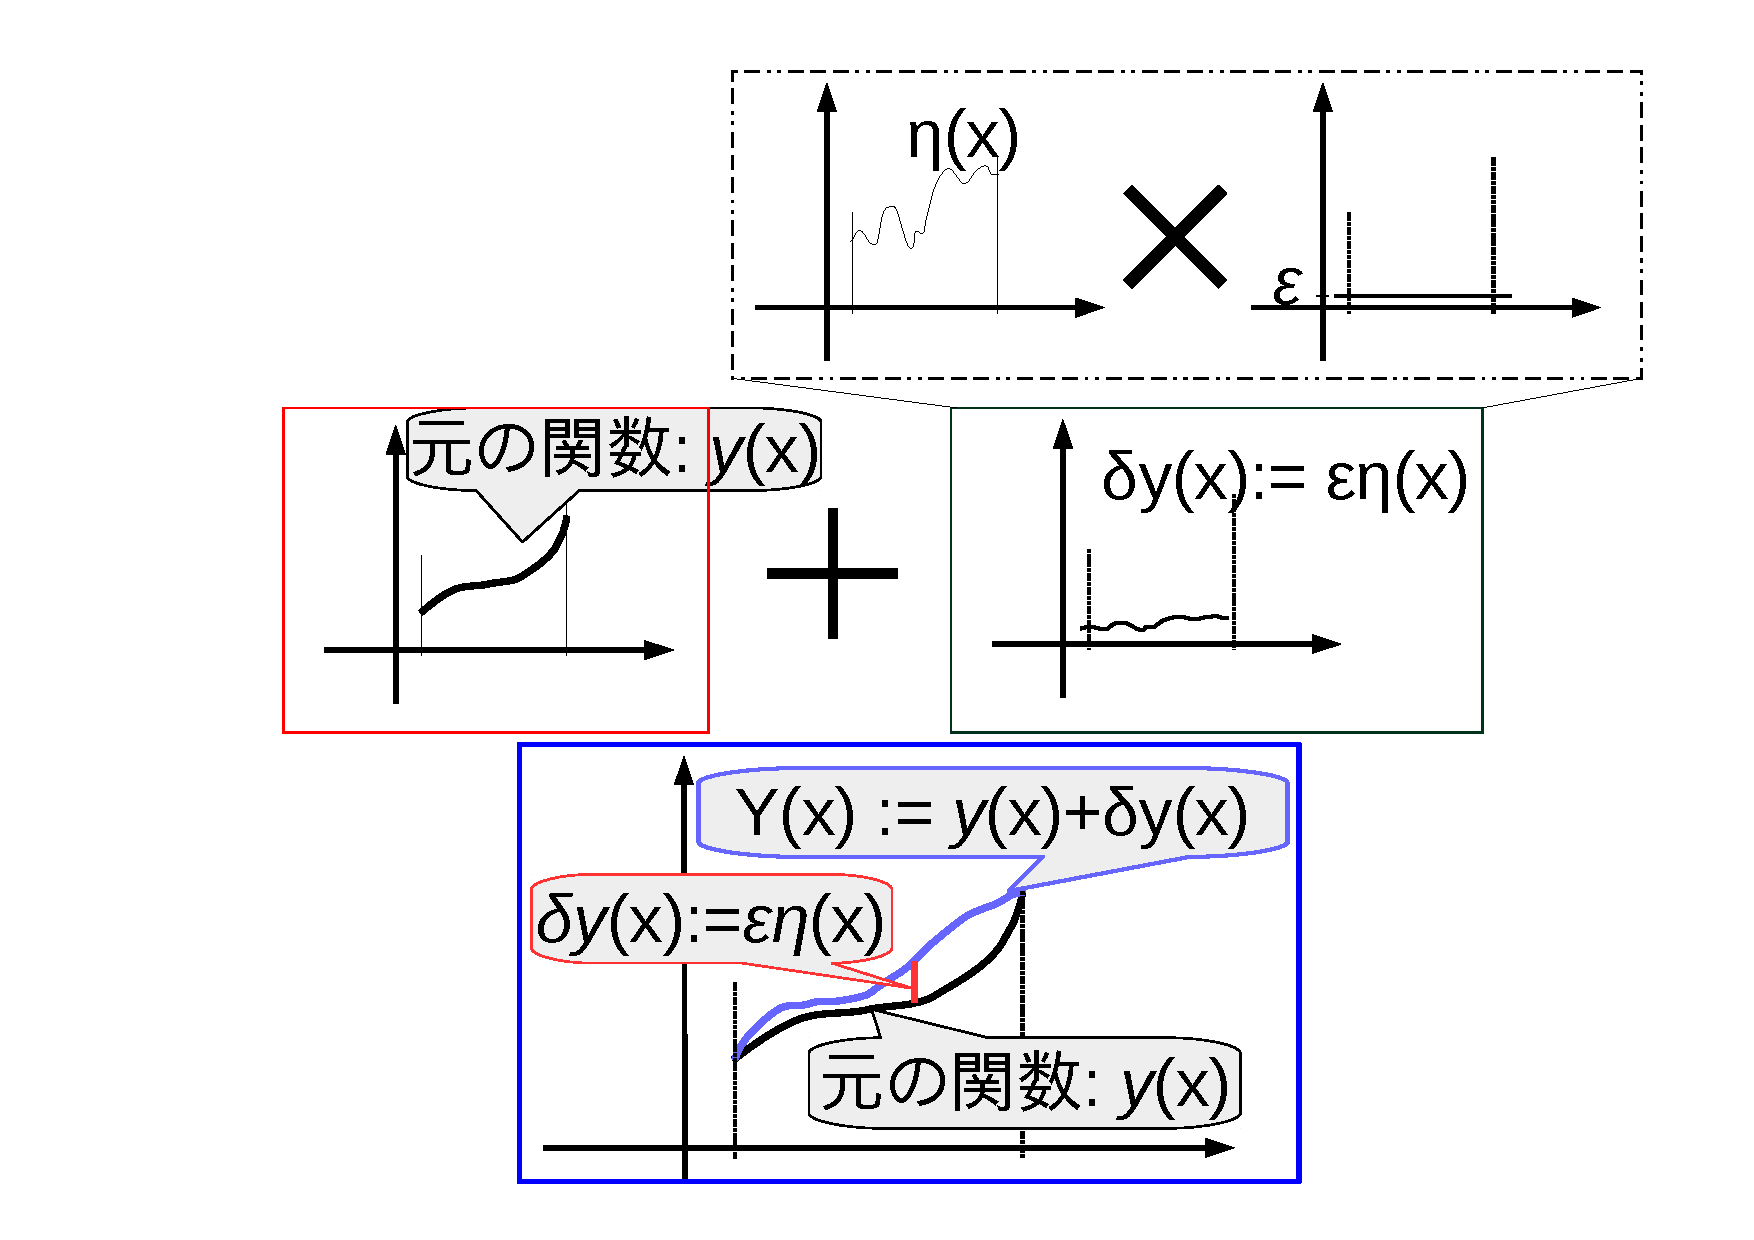
\includegraphics[keepaspectratio, width=7.5cm,height=6.9cm,clip]{henbun1.pdf}
                                \caption{変分のイメージ}
                                \label{fig:henbun1}
                            \end{center}
                        \end{figure}
                \end{mysmallsec}

                \begin{mysmallsec}{多変数関数の場合}
                    変数が2つある場合,すなわち,$f(x,\,y)$ に対する変分について,考えよう.
                    1変数の場合に真似して,以下のような関数 $F(x,\,y)$ を導入する.
                        \begin{align}
                            F(x,\,y) = f(x,\,y) + \varepsilon \eta(x,\,y).
                        \end{align}
                    ここで,$\varepsilon$ は任意の小さな実数で,$\eta(x,\,y)$ は任意の関数である.
                    さらに1変数の場合と同様に,2変数関数の変分 $\delta f(x,\,y)$ を以下のように与える.
                        \begin{align}
                            \delta f(x,\,y) := \varepsilon \eta(x,\,y) = F(x,\,y) - f(x,\,y).
                        \end{align}
                    これを使って,以下のように書き直しておく.
                        \begin{align}
                            F(x,\,y) = f(x,\,y) + \delta f(x,\,y).
                        \end{align}
                    3変数以上の多変数関数についても,同じように定義できる.
                        \begin{align}
                            \delta f(x,\,y,\,\cdots) &:= \varepsilon \eta(x,\,y,\,\cdots) \notag \\
                                                     &= F(x,\,y,\,\cdots) - f(x,\,y,\,\cdots).
                        \end{align}

                        独立変数の個数にかかわらず,同様に定義できるので,
                    独立変数の記述を省略して一般性を高めた記述にでき,
                        \begin{equation*}
                            \delta f := \varepsilon \eta = F - f
                        \end{equation*}
                    と書かれることになる.この場合,$F$ や $f$ が関数であることは前もって
                    定義しておかないといけない.
                \end{mysmallsec}

%           %==================================================================
%           %  SubsubSection
%           %==================================================================
            \subsubsection{汎関数の微分}
                汎関数は関数をその定義域として持つ関数であり,汎関数の微分と言われると,
                簡単にはイメージできない.関数 $f(x)$ を独立変数に持つ汎関数 $I[f(x)]$ を
                関数 $f(x)$ で微分する場合,
                    \begin{equation*}
                        \frac{\delta I[f(x)]}{\delta f(x)}
                        = \lim_{\delta f(x) \to 0}
                          \frac{I[f(x)+\delta f(x)] - I[f(x)]}{\delta f(x)}
                    \end{equation*}
                と書かれる.$\delta f(x) \to 0$ とかかれても意味がわからないので,非常に小さい実数 $\varepsilon$ と
                任意関数 $\eta(x)$ を導入し,$\delta f(x):= \varepsilon \eta(x)$ として置き換えてみよう.
                    \begin{equation*}
                        \frac{\delta I[f(x)]}{\delta f(x)}
                        = \lim_{\varepsilon \eta(x) \to 0}
                          \frac{I[f(x)+\varepsilon \eta(x)] - I[f(x)]}{\varepsilon \eta(x)}
                    \end{equation*}
                残念ながら,これではうまく微分を定義できそうにない.しかし,頭のいい人はいるもので,
                汎関数の微分を定義した人がいる.その人の名前をとって,\textbf{ガトー微分} と言われる
                    \footnote{
                        Ren\'{e} Eug\`{e}ne G\^{a}teux(1889--1914, フランス):
                        ここで紹介している通り,\textbf{ガトー微分} としてその名を残ししたフランスの
                        数学者.第一次世界大戦で命を落とした.
                    }.
                それは以下のように定義される.
                    \begin{align}
                        \frac{\delta I[f(x)]}{\delta f(x)}
                        := \lim_{\varepsilon \to 0} \frac{I[f(x)+\varepsilon \eta(x)] - I[f(x)]}{\varepsilon}.
                    \end{align}
                言葉にしてみれば,「汎関数 $I[f(x)]$ の関数 $f(x)$ における $\eta(x)$ に対する微分」となる
                    \footnote{
                        いきなりこれを聞いたら,思考停止するだろう.ナンノコッチャ,サッパリわからない.
                        しかし,一度は,ガトー微分の定義式と見比べながら,その意味をゆっくり消化していって欲しい.
                        ちゃんと意味のあることを言っている(意味不明ではない).
                    }.



%           %==================================================================
%           %  SubsubSection
%           %==================================================================
            \subsubsection{汎関数の変分}
                \begin{mysmallsec}{1変数関数の場合}
                    1変数関数をその引数としてもつ汎関数 $I = I[f(x)]$ を考える.
                    この汎関数 $I[f(x)]$ に対して,関数 $f(x)$ にその変分を加えた $f(x) + \delta f(x)$ を
                    代入し,$I[f(x)+\delta f(x)]$ を作る.$I[f(x)+\delta f(x)]$ と元の $I[f(x)] $ の
                    差分を汎関数 $I$ の変分といい,同様に $\delta I$ とかく.
                        \begin{align*}
                            \delta I := I[f(x)+\delta f(x)] - I[f(x)].
                        \end{align*}
                    上では,関数 $f$ を1変数関数としたが,多変数でもかまわない.なので,引数の記述を
                    省略して,以下のように記述されることが多い.
                        \begin{align}
                            \delta I := I[f+\delta f] - I[f].
                        \end{align}
                \end{mysmallsec}

                \begin{mysmallsec}{多変数関数の場合}
                    独立変数としての関数を複数もつ汎関数に対する変分も,1変数の場合に真似て定義すればいい.
                        \begin{align}
                            \delta I :=   I[f_{0}+\delta f_{0}, f_{1}+\delta f_{1}, \cdots]
                                        - I[f_{0}, f_{1}, \cdots].
                        \end{align}
                \end{mysmallsec}

%           %==================================================================
%           %  SubsubSection
%           %==================================================================
            \subsubsection{正準方程式の導出}
                ラグランジアン $L$ は位置 $\br$ と速度 $\dot{\br}$ の関数であるので,
                その変分は以下のように書ける
                    \footnote{
                        左辺の $L$ は独立変数を明示したが,右辺の $L$ は式の煩雑さを避けるために
                        独立変数表記を省略した.以下,ラグランジアン $L$ は位置と運動量の関数である
                        として,独立変数の表記を省略する.
                    }.
                    \begin{equation*}
                        \delta L(\br,\,\dot{\br}) =   \frac{\rd L}{\rd \br}\delta \br
                                                    + \frac{\rd L}{\rd \dot{\br}}\delta \dot{\br}.
                    \end{equation*}
                この式に対して,
                一般化運動量 $\bp = \rd L/\rd \dot{\br}$ と
                一般化された力 $F=\dot{\bp} = \rd L/\rd \br$ を考慮すると,
                    \begin{equation*}
                       \delta  L =  \dot{\bp} \cdot \delta \br + \bp \cdot \delta \dot{\br}.
                    \end{equation*}
                ここで,変分の公式
                    \begin{equation*}
                        \delta(\bp\cdot\dot{\br}) = \bp\cdot\delta\dot{\br} + \dot{\br}\cdot\delta\bp
                    \end{equation*}
                を考える.この変分公式から,さっき計算した $L$ を引くと,
                    \begin{align*}
                        \delta(\bp\cdot\dot{\br}) - \delta L &= \dot{\br}\cdot \delta\bp - \dot{\bp} \cdot \delta \br
                    \end{align*}
                となる.左辺は $\delta$ で囲んでおこう.
                    \begin{align*}
                        \delta(\bp\cdot\dot{\br} - L) &= \dot{\br}\cdot \delta\bp - \dot{\bp} \cdot \delta \br
                    \end{align*}
                そして,左辺に現れた$\bp \cdot \dot{\br} - L$ に対して,これを \textbf{ハミルトニアン} と定義する.
                記号は $H$ とする.
                    \begin{equation*}
                        H := \bp \cdot \dot{\br} - L.
                    \end{equation*}
                ハミルトニアンを使うと,
                    \begin{align}\label{eq:HamiltonianBrp}
                        \delta H = \dot{\br}\cdot\delta\bp - \dot{\bp} \cdot\delta \br.
                    \end{align}

                この式から,ハミルトニアン $H$ のもつ独立変数は,$\bp$ と $\br$ であるといってよい.
                つまり,一般に,ハミルトニアンの変分 $\delta H$ は以下のように計算される.
                    \begin{align}\label{eq:HamiltonianZenbibun}
                        \delta H = \frac{\rd H}{\rd \bp}\delta \bp + \frac{\rd H}{\rd \br}\delta \br.
                    \end{align}

                式(\ref{eq:HamiltonianBrp})と式(\ref{eq:HamiltonianZenbibun})を見比べてみると,
                以下の関係が成立していることが見て取れる.
                    \begin{align}
                        \frac{\rd H}{\rd \bp} &= \dot{\br} \\
                        \frac{\rd H}{\rd \br} &= - \dot{\bp}.
                    \end{align}
                この2つの式はハミルトンの \textbf{正準運動方程式} と呼ばれる
                    \footnote{
                        本当のことをいうと,この方程式は正式な正準運動方程式
                        とはいえない.という言うのも,一般化座標を定義せずに
                        直交座標で感がてしまっているからである.しかし,
                        一般化座標も直交座標も形式的には全く同じ形で
                        表現されるので,ここで表れている位置座標を
                        一般化座標と同一視することができ,この式を
                        正準運動方程式と呼んでも差支えないのである.
                        一般化座標については,後でより詳しく解析力学を
                        学習するときに定義する.
                    }.

        \begin{memo}{変分と微分の可換性}
            変数 $x$ を独立変数とする関数 $f(x)$ を考える.
            この関数からほんの少しだけずれた値を持つ関数を仮想的に考えて,これを$F(x)$ とする.
            この時,
                \begin{align}\label{eq:henbun1}
                    F(x) = f(x) + \delta f(x)
                \end{align}
            となるように,$\delta f(x)$ を導入する
                \footnote{
                    $\delta f(x)$ のことを \textbf{変分} とよぶのであった.
                }.

            ここで確認したいのは,
                    「(1) 微分してから,その微分の変分をとる」ことと,
                    「(2) 変分をとってから,その変分を微分する」ことが,
            同じ結果を導くということだ. 要するに,
                「微分と変分の順番を入れ替えても結果が変わらない」
            ということを確認したいのである.式で書けば,
                \begin{equation*}
                    \delta \left( \frac{\df}{\df x} f(x) \right) = \frac{\df}{\df x}\delta f(x)
                \end{equation*}
            である.本当にそうなるか.確認してみよう.
            上の左辺を式変形していき,右辺に帰着させる
                \footnote{
                    もちろん,右辺から左辺へ式変形してもいい.
                    その場合,ここでの計算式を逆にたどったものになる,
                }.
            難しいことは何もない.微分と変分の定義に従って式変形していくだけでいい.
            実際の計算が以下になる.
                \begin{align*}
                    \mbox{} &         \delta \left( \frac{\df}{\df x} f(x) \right) \\
                            & \quad = \delta \left( \lim_{\Delta x \to 0} \frac{f(x+\Delta x) - f(x)}{\Delta x} \right) \\
                            & \quad = \left( \lim_{\Delta x \to 0} \frac{F(x+\Delta x) - F(x)}{\Delta x} \right) \\
                            &         \qquad \qquad  - \left( \lim_{\Delta x \to 0} \frac{f(x+\Delta x) - f(x)}{\Delta x} \right) \\
                            & \quad = \lim_{\Delta x \to 0}
                                      \frac{F(x+\Delta x) - F(x) - f(x+\Delta x) +  f(x) }{\Delta x} \\
                            & \quad = \lim_{\Delta x \to 0}
                                      \frac{F(x+\Delta x) - f(x+\Delta x) - F(x) +  f(x) }{\Delta x} \\
                            & \quad = \lim_{\Delta x \to 0}
                                      \frac{ \left( F(x+\Delta x) - f(x+\Delta x) \right)- \left( F(x) -  f(x) \right)}{\Delta x} \\
                            & \quad = \lim_{\Delta x \to 0}
                                      \frac{ \delta f(x+\Delta x) - \delta f(x)}{\Delta x} \\
                            & \quad = \lim_{\Delta x \to 0}
                                      \frac{ \delta \left( f(x+\Delta x) - f(x) \right)}{\Delta x} \\
                            & \quad = \frac{\df}{\df x}\delta f(x).
                \end{align*}
            これで変分と微分の可換性が示せた.

            同じことだが,もしかしたら省略記号で書いたほうが証明が読みやすいかもしれない.
                \[
                    \delta \left( \frac{\df f}{\df x} \right) = \frac{\df (f + \delta f)}{\df x} - \frac{\df f}{\df x} = \frac{\df (\delta f)}{\df x} = \frac{\df }{\df x} (\delta f).
                \]
            もしくは,$F=f+\delta f$とすれば$\delta f = F - f$であり,以下のようにも示せる.
                \[
                    \delta \left( \frac{\df f}{\df x} \right) = \frac{\df F}{\df x} - \frac{\df f}{\df x} = \frac{\df (F-f)}{\df x} = \frac{\df (\delta f)}{\df x} = \frac{\df }{\df x} (\delta f).
                \]
            
            

        \end{memo}

%   %==========================================================================
%   %  Section
%   %==========================================================================
    \section{変分原理}
%       %======================================================================
%       %  SubSection
%       %======================================================================
        \subsection{学習マップ}
            これから,最小作用の原理という考え方を使って,もう一度,
            ラグランジュの運動方程式を導出する.先ほどの導出方法は,
            少々強引な所があったが,最小作用の原理を使った導出方法は
            いくらか自然なものと感じることだろう.

            話が長く,その順が把握しづらくなってしまうので,
            その過程を箇条書きをしておこう.
                \begin{enumerate}
                    \item ダランベールの原理
                    \item 仮想仕事の原理
                    \item 最小作用の原理
                    \item ラグランジュの運動方程式の導出
                    \item ネーターの定理と対称性の確認
                    \item ハミルトニアンの導入(ラグランジアンのルジャンドル変換)
                    \item 正準運動方程式(ハミルトン形式の運動方程式)
                \end{enumerate}

            この順番が,話の流れが自然だと思う.
            解析力学のほとんどの教科書が,この順で説明されている.

            以降の話は,少々数学的な話になってしまうが,我慢して学習を
            しよう.解析力学がとても綺麗に整っている理論であること,
            一般性が高いということ等を実感できることだろう.

%       %======================================================================
%       %  SubSection
%       %======================================================================
        \subsection{ダランベールの原理}
            $\ddot{\br}$ を用いると運動方程式は
                \begin{align}
                    m\ddot{\br} = \bF
                \end{align}
            と書ける.この式の $m\ddot{\br}$ を右辺に移行して,
                \begin{align}
                    \bF-m\ddot{\br} = 0
                \end{align}
            となる.ここで,$\bar{\bF} := \bF-m\ddot{\br}$ とおくと,
                \begin{align}
                    \bar{\bF} = 0
                \end{align}
            とかける.この式は物体に力が加わっていない状態を表す.つまり,以下のように解釈できる.
                \begin{myshadebox}{ダランベールの原理}
                    運動している物体に $-m\ddot{\br}$ の力が加わえると,あたかも
                    それが力 $\bF$ と釣り合って,静止しているようにみなせる.
                \end{myshadebox}

            このような解釈を,\textbf{ダランベールの原理} という.

%       %======================================================================
%       %  SubSection
%       %======================================================================
        \subsection{仮想仕事の原理}
            静止している物体は,ダランベールの原理により,$\bF-m\ddot{\br} = 0$ と
            表せる.この式の両辺に,仮想的な変位(\textbf{仮想変位})$\delta\br (\neq0)$ をかける.
                \begin{align}\label{k_sigo}
                    \left(\bF-m\ddot{\br}\right)\cdot\delta\br  = 0
                \end{align}
            この式は,\textbf{仮想仕事の原理} とよばれる.

%       %======================================================================
%       %  SubSection
%       %======================================================================
        \subsection{ラグランジアン と 最小作用の原理}
            \begin{mycomment}
            仮想仕事の原理から,物体の運動の規則性を見つけることができる.
            そのために,ある曲面上で始点Aと終点Bを決める.
            始点Aは終点Bよりもポテンシャルが高い位置であるとする.
            このとき,物体を始点Aから離してポテンシャルのみによって
            終点Bに変位する状況を考える.どのような径路で物体はAからBへ移動するだろうか.
            実際に,何回もAからBへ物体を移動させたところで,外力が働かない限り,
            径路は変わることはない.つまり何らかの規則があることが予想される.
            この規則をここで考えてきたいと思う.
            \end{mycomment}

            仮想仕事の原理の式(\ref{k_sigo})の両辺を時間で積分する.その際,
            積分範囲は,$\delta \br(t_{1})=\delta\br(t_{2})=0$ を
            満たす $t_{1}$ から $t_{2}$ を用意
            して, $t_{1}$ から $t_{2}$ で積分する.イメージを言えば,始点Aが $\br(t_{1})$ にあたり,
            終点Bが $\br(t_{2})$ にあたる.これらを 0 としたのは,
            始点と終点が固定されているとを仮定するからである.
                \begin{align}
                    \begin{cases}
                        \displaystyle \int_{t_{1}}^{t_{2}}\left(\bF
                        -m\ddot{\br}\right)\cdot\delta\br \df t = 0 \\
                        \displaystyle \delta\br(t_{1})=\displaystyle \delta \br(t_{2})= 0
                    \end{cases}
                \end{align}
                \begin{align}
                        \displaystyle \int_{t_{1}}^{t_{2}}\bF\cdot\delta\br\df t+
                        \int_{t_{1}}^{t_{2}}-m\ddot{\br}\cdot\delta\br \df t = 0
                \end{align}
            この式の 右辺第2項 を部分積分して,
                \begin{align}
                        \mbox{}
                        &  \int_{t_{1}}^{t_{2}}-m\ddot{\br}\cdot\delta\br \df t \notag \\
                        &= \Bigl[ -m\dot{\br}\cdot\delta\br \Bigr]_{t_{1}}^{t_{2}}
                           -\int_{t_{1}}^{t_{2}} \left(-m\dot{\br}\cdot \frac{\df }{\df t} \delta\br \right) \df t.
                \end{align}
            ここで,$\Bigl[ -m\dot{\br}\cdot\delta\br \Bigr]_{t_{1}}^{t_{2}}$ の
            項は,$\delta \br(t_{1})=\delta\br(t_{2})=0$ により,0 になる.よって,
                \begin{align}
                        \int_{t_{1}}^{t_{2}}\bF\cdot\delta\br\df t+
                        \int_{t_{1}}^{t_{2}}
                        \left(m\dot{\br}\cdot \frac{\df }{\df t} \delta\br \right) \df t &= 0 \notag \\
                        \Leftrightarrow \quad
                        \int_{t_{1}}^{t_{2}}\bF\cdot\delta\br\df t+
                        \int_{t_{1}}^{t_{2}}
                        \left(m\dot{\br}\cdot\delta \dot{\br} \right) \df t &= 0
                \end{align}
            と計算できる.

            ところで,
                \begin{align}
                    m\dot{\br}\cdot\delta \dot{\br} =
                    \frac{1}{2}m\delta(\dot{\br})^{2}=
                    \delta\left(\frac{1}{2}m\dot{\br}^{2}\right)
                \end{align}
            の関係を用いれば,
                \begin{align}
                        \delta\int_{t_{1}}^{t_{2}}\bF\cdot\br\df t+
                        \delta\int_{t_{1}}^{t_{2}}
                        \left(\frac{1}{2}m\dot{\br}^{2}\right)\, \df t = 0
                \end{align}
            である.ここで,仕事 $W=\bF\cdot\br$,
            運動エネルギー $T=m\dot{\br}^{2}/2$ を用いて,
                \begin{align}
                        \delta\int_{t_{1}}^{t_{2}}W\df t+
                        \delta\int_{t_{1}}^{t_{2}}T\df t &= 0 \notag \\
                        \Leftrightarrow
                        \delta\int_{t_{1}}^{t_{2}}\left(W+T\right) \df t &= 0
                \end{align}
            と書ける.

            力がポテンシャルのみにより導かれるならば,この式の $W$ はポテンシャル$\cdot$エネルギーと同等であり,$W=-U$ と
            書き換えれば,
                \begin{align}
                        \delta\int_{t_{1}}^{t_{2}}\left(T-U\right) \df t &= 0
                \end{align}
            を得る.さらに,ラグランジアン $L$ を
                \begin{align}
                    L := T-U
                \end{align}
            と定義すると,
                \begin{align}
                        \delta\int_{t_{1}}^{t_{2}}L  \df t &= 0
                \end{align}
            を得る.そして最後に,\textbf{作用} を
                \begin{align}
                        S := \int_{t_{1}}^{t_{2}}L \df t
                \end{align}
            と定義すると,
                \begin{align}
                    \delta S = 0
                \end{align}
            となる.これを \textbf{最小作用の原理} という.

            言葉で言うならば,
            物体は作用 $S$ の変分 $\delta S$ が最小になるような軌道で運動する,
            となる.

            幾つかの重要な概念が出てきた.まとめておこう.
                \begin{myshadebox}{ラグランジアン}
                    ラグランジアン $L$ を次式で定義する.
                        \begin{align}
                            L := T-U
                        \end{align}
                \end{myshadebox}
                \begin{myshadebox}{作用}
                    作用 $S$ を次式で定義する.
                        \begin{align}
                            S := \int_{t_{1}}^{t_{2}}L \df t
                        \end{align}
                \end{myshadebox}
                \begin{myshadebox}{最小作用の原理}
                    物体は作用 $S$ の変分 $\delta S$ が最小になるような
                    軌道で運動する.これを \textbf{最小作用の原理} といい,
                    次式で表される.
                    \begin{align}\label{s_sigo}
                        \delta S = 0.
                    \end{align}
                \end{myshadebox}

            \begin{memo}{ラグランジアンの定義について}
                ここで定義したラグランジアン $L$ は,
                運動エネルギー $T$ とポテンシャル$\cdot$エネルギー $U$ で表
                され,具体的には $L=T-U$ である.
                運動エネルギー $T$ は速度 $\dot{\br}(t)$ と時間 $t$ だけの関数であり,
                $T=T(\dot{\br}(t),\,t)$ と表現でき,また,ポテンシャル$\cdot$エネルギー $U$ は
                位置 $\br(t)$ と時間 $t$ だけの関数であり,$U=U(\br(t),\,t)$ と書ける.
                すなわち,ラグランジアン $L$ は $T(\dot{\br}(t),\,t)$ と $U(\br(t),\,t)$ から
                定義される量であり,
                    \begin{align}
                        L =L (\br(t),\dot{\br}(t),t)
                    \end{align}
                と書けることがわかる.つまり,ラグランジアンは,位置座標と速度,時間の3つの独立変数をもつ
                関数であると言える.

                さて,このように定義されるラグランジアン
                は \textbf{速度と位置座標と時間は独立な変数として扱っている} ことに注意する.
                速度の定義は位置座標の時間微分であって,従って,
                位置座標や時間とは独立ではないと考えられるが,
                ラグランジュ形式の力学では,あたかも位置座標と速度と
                時間が互いに独立な変数として扱うのである.
            \end{memo}

            \begin{memo}{最小作用の原理のイメージ}
                最小作用の原理が意味することは,物体が運動する時には作用が極大または極小になるような
                軌道を描くということである.ただそれだけのことを記述しているのである.従って,
                作用とは何かについては,教えてくれない.しかし,この作用という抽象的な概念さえ
                認めることができれば,力学の理論は“スマート”に記述できるのである.もっといえば,
                この作用というのは力学だけにとどまるものではなく,物理学全体にかかわるとても
                重要な概念である.従って,「作用」という具体的なイメージを
                つかめなくても,そのようなものが“存在”すると考えるのである.
                そうすれば,物理現象を統一的に扱える可能性が見出せるかもしれない..
            \end{memo}

%       %======================================================================
%       %  SubSection
%       %======================================================================
        \subsection{ラグランジュの運動方程式の導出}
            \textbf{これ以降の式変形は,単に形式的に考え,物理的または
            数学的意味は(とりあえず)考えないようにする}.

            前項目のように定義した $S$ は
            関数 $L$ を変数とする汎関数である.このことを $S[L]$ のように表現する.

            ここでは,
                \begin{align}
                    S[L]=\int L(\br(t),\dot{\br}(t),t) \df t
                \end{align}
            と表される汎関数 $S$ について考える.積分方程式と考えることもできる.

            $\br$ と $\dot{\br}$ は独立な変数であるとして扱う.
            積分区間を,$t_{1}$ から $t_{2}$ とする.
            ここで,$\delta\br(t_{1})=\delta\br(t_{2})$ となるようにする.
                \begin{align}
                    \begin{cases}
                        \displaystyle S[L]  &= \displaystyle\int_{t_{1}}^{t_{2}} L \df t = \displaystyle\int_{t_{1}}^{t_{2}}
                        L(\br(t),\dot{\br}(t),t) \df t \\
                        \displaystyle \delta\br(t_{1}) &= \delta\displaystyle \br(t_{2})
                    \end{cases}
                \end{align}

            ここで,$L$ が微小変化して $L+\delta L$ になったときの, $S$ の
            変化 $\delta S$ を考える.$\delta S$ は次の様に定義される.
                                \begin{align}
                        \delta S:=S[L+\delta L]-S[L]
                                \end{align}

                        作用 $S[L]$ は定義そのものであり,
                        \begin{align*}
                                S[L]          &= \int_{t_{1}}^{t_{2}} L \df t.
                        \end{align*}
                        同じように,$S[L+\delta L]$ は
                        \begin{align*}
                                S[L+\delta L] &=  \int_{t_{1}}^{t_{2}} \left(L + \delta L\right)\df t. \\
                                                                  &=  \int_{t_{1}}^{t_{2}} L \df t + \int_{t_{1}}^{t_{2}} \delta L \df t.
                        \end{align*}
            よって,
                \begin{align*}
                        \delta S := S[L+\delta L] - S[L] = \int_{t_{1}}^{t_{2}} \delta L \df t.
                \end{align*}
                        清書して,
                \begin{align}
                        \delta S = \int_{t_{1}}^{t_{2}} \delta L \df t.
                \end{align}

            $\delta L$ はテイラー展開を使って,
                \begin{align}
                    \delta L=\frac{\rd L}{\rd \br}\delta \br
                            +\frac{\rd L}{\rd \dot{\br}}\delta\dot{\br}
                            +\frac{\rd L}{\rd t}\delta t
                \end{align}
            であるから,$\delta S$ は
                \begin{align}
                    \delta S&= \int_{t_{1}}^{t_{2}}\left(
                                        \frac{\rd L}{\rd \br}\delta \br
                                        +\frac{\rd L}{\rd \dot{\br}}\delta\dot{\br}
                                        +\frac{\rd L}{\rd t}\delta t \right) \df t
                \end{align}
            と書ける.

            さらに,ラグランジュ関数 $L$ は時間変化しないとし,右辺第3項の時間積分の項は0になると考えて,
            次のように変形する.
                \begin{align}\label{deltax}
                                \delta S&= \int_{t_{1}}^{t_{2}}\left(
                                          \frac{\rd L}{\rd \br}\delta \br
                                          +\frac{\rd L}{\rd \dot{\br}}\delta\dot{\br}
                                          \right) \df t.
                \end{align}

            さて,この式の右辺第2項の $(\rd L/\rd \dot{\br})\delta\dot{\br}$ の $\delta\dot{\br}$ の部分に注目して,
                \begin{align}\label{deltax2}
                    \delta\dot{\br}=\delta\frac{\df\br}{\df t}=\frac{\df }{\df t}\delta \br
                \end{align}
            であることから,式(\ref{deltax2})を式(\ref{deltax})にこれを代入して,
                \begin{align}\label{eq:deltax3}
                    \delta S&=  \int_{t_{1}}^{t_{2}}\left(
                                            \frac{\rd L}{\rd \br}\delta \br
                                                +\frac{\rd L}{\rd \dot{\br}}\frac{\df }{\df t}\delta \br
                                            \right) \df t \notag \\
                                                        &=  \int_{t_{1}}^{t_{2}}
                                                            \left( \frac{\rd L}{\rd \br}\delta \br \right) \df t
                                                           +\int_{t_{1}}^{t_{2}}
                                                            \left( \frac{\rd L}{\rd \dot{\br}}\frac{\df }{\df t}\delta \br \right) \df t
                \end{align}
            さらに,この式の右辺第2項に部分積分を適用して,
                \begin{align*}
                                \mbox{}
                        &  \int_{t_{1}}^{t_{2}} \left( \frac{\rd L}{\rd \dot{\br}}\frac{\df }{\df t}\delta \br \right) \df t \\
                    &= \Bigl[\frac{\rd L}{\rd\dot{\br}}\delta \br\Bigr]_{t_{1}}^{t_{2}}
                      -\int_{t_{1}}^{t_{2}}\frac{\df }{\df t} \frac{\rd L}{\rd \dot{\br}} \delta \br\df t.
                \end{align*}

            仮定により $\delta\br(t_{1}) =\delta \br(t_{2})$ であるから,
                \begin{align*}
                    \Bigl[\frac{\rd L}{\rd\dot{\br}}\delta \br\Bigr]_{t_{1}}^{t_{2}}
                    = \frac{\rd L}{\rd\dot{\br}}\delta \br(t_2) - \frac{\rd L}{\rd\dot{\br}}\delta \br(t_{1})
                    = 0
                \end{align*}
            となって,以下になる.
                                \begin{align*}
                                        \int_{t_{1}}^{t_{2}}\left( \frac{\rd L}{\rd \dot{\br}}\frac{\df }{\df t}\delta \br \right) \df t
                    = -\int_{t_{1}}^{t_{2}}\frac{\df }{\df t} \frac{\rd L}{\rd \dot{\br}} \delta \br\df t.
                                \end{align*}

                        これより,式(\ref{eq:deltax3})は次の通り
                \begin{align}
                    \delta S&=\int_{t_{1}}^{t_{2}}\left(
                    \frac{\rd L}{\rd \br}\right) \delta \br\df t
                    -\int_{t_{1}}^{t_{2}}\frac{\df }{\df t} \frac{\rd L}{\rd \dot{\br}}
                    \delta \br\df t.
                \end{align}
                        右辺の2つの項の積分範囲は同一であり,1つにまとめられる.
                \begin{align}
                    \delta S&=\int_{t_{1}}^{t_{2}}\left(
                    \frac{\rd L}{\rd \br}
                    -\frac{\df }{\df t} \frac{\rd L}{\rd \dot{\br}}
                    \right)\delta \br\df t.
                \end{align}

            最後に,最小作用の原理($\delta S$ が極値をとると考えれば,$\delta S=0$)を導入して,
                \begin{align*}
                    \delta S = \int_{t_{1}}^{t_{2}}\left(
                                                 \frac{\rd L}{\rd \br}
                                                -\frac{\df }{\df t} \frac{\rd L}{\rd \dot{\br}}
                                            \right)\delta \br\df t
                                         = 0.
                \end{align*}
            これが成り立つためには,被積分関数が0になる場合であり,
                \begin{align}
                    \frac{\rd L}{\rd \br} -\frac{\df }{\df t} \frac{\rd L}{\rd \dot{\br}}=0
                \end{align}
            である.この式が直交座標の \textbf{ラグランジュの運動方程式} である.

                \begin{center}
                    \begin{itembox}[l]{\textbf{ラグランジュの運動方程式}(直交座標系)}
                        \begin{align}
                            \frac{\rd L}{\rd \br}
                            -\frac{\df }{\df t} \frac{\rd L}{\rd \dot{\br}}=0
                        \end{align}
                    \end{itembox}
                \end{center}

            \begin{memo}{共変性}
                実はラグランジュの運動方程式は,直交座標でなくとも,任意の
                座標を用いてもその方程式の形を変えない.このようなことを
                座標変換に対して \textbf{共変} であるという.
                そこで,次の節で,座標系の変換について考え,
                ラグランジュの運動方程式の座標に対して共変性をもつことを
                確認する.
            \end{memo}

%       %======================================================================
%       %  SubSection
%       %======================================================================
        \subsection{一般化座標}
            物体の位置は複数の座標系で表現できることは前に確認している.
            どの座標系を用いて運動方程式をたてるかは人間が任意に決定するものであって,
            自然とは本来,人間とは関係なく存在しているので,
            座標系を人間が勝手に選ぶということは好ましくない.
            確かに,どのよな座標系を選んでも,
            物体の運動軌道は一致するが,
            その表現方法や,運動方程式の形はそれぞれ異なる.
            自然法則が表現方法によって異なった形になってしまうとは到底
            考えにくい.そうなってしまうのは,人が都合のよいように
            座標系を選んでしまうからである.そこで,
            座標系をより一般的なものに拡張しようと考える.
            この一般的な座標とは,任意の座標系の代表であり,
            どのような座標系でもかまわない.
            そのような座標系を \textbf{一般化座標} という.

            一般化座標を表現する記号は $q$ が用いられる.
            例えば,3次元の一般化座標は番号を $q$ の
            右上にそえて,($q^{1}$, $q^{2}$, $q^{3}$) のように書く.
            これは直交座標での ($x$, $y$, $z$) に相当するものである.
            $N$ 個の物体を扱うときはこの分だけ変数が増えることになる.
            具体的には変数は $3N$ 個ということになる.
            つまり,必要な座標は
            \begin{equation*}
                (q^{1}, q^{2}, \cdots , q^{3N-1}, q^{3N})
            \end{equation*}
            ということになる.しかし,これではあまりにも冗長なので,
            自然数を代表する文字 $i$ を導入して,
            \begin{equation*}
                q^{i} , (i=1, 2, \cdots, 3N)
            \end{equation*}
            と表現する
                \footnote{
                    ここでの $i$ は任意の自然数を表現する記号である.
                    同じ文字を,異なった分野で用いることは多々あるが,
                    それぞれ全く異なるものであり,関係はない.
                    例えば,$i$ は電磁気学では電流を
                    表現する記号として用いられる.
                    今使用している文字がどのような意味で用いられて
                    いるがを
                    注意しておく必要がある.$i$ と書かれていたからといって,
                    自然数であると勝手に思い込んではいけない.
                    また,教科書によって多少の記号の用いられかたが
                    異なっているので,その約束に従って読むことである.
                }.
            以後,($i=1, 2, \cdots, 3N$) を省略する
            場合の多いが,そのときは適宜解釈をしてほしい.

%       %======================================================================
%       %  SubSection
%       %======================================================================
        \subsection{運動方程式の共変性}
            上ではラグランジュの運動方程式を直交座標系で表現したが,
            実はラグランジュの運動方程式は直交座標系に限らず,
            極座標系でも円筒座標系でも,一般の座標系で
            その形を変えずに成り立つ
                \footnote{
                    ニュートンの運動方程式は直交座標系で書いたものと
                    曲座標系で書いたものは形が異なってしまうことが多い.
                }.
            このように,座標変換によって変数変換をしても
            その方程式の形を変えないことを,座標変換に対して \textbf{共変} であるといい,
            そのような方程式は座標変換に対して \textbf{共変性} をもつという.

            ここでは,ラグランジュの運動方程式が直交座標系で成り立つときに,
            一般の座標でも運動方程式の形が変わることなく成立することを
            確認する.

            ある座標系(これを $q^{i}$ とする)でラグランジュの運動方程式が書かれているとする.
            このときのラグランジアンを $L$ として,
                                    \begin{align}\label{eq:ラグランジュ1}
                                        \frac{\rd L}{\rd q^{i}}
                                        -\frac{\df }{\df t} \frac{\rd L}{\rd \dot{q}^{i}}=0
                                    \end{align}
            である.
            この座標系とは別の座標系に変換するとき,
                \begin{align}\label{eq:henkan}
                    q^{i}=\phi^{i} (\bar{q}^{i},\,t)
                \end{align}
            で変換されるとする.この変換は点変換とよばれる.
            ラグランジュの運動方程式は
            この点変換に対してその形を変えないのである.これを今から確認する.


            座標 $q^{i}$ の全微分 $dq^{i}$ は,
                \begin{align*}
                    dq^{i} = \sum_{k=1}^{3N}\left(\frac{\rd \phi^{i}}{\rd \bar{q}^{k}}\df\bar{q}^{k}\right)+\frac{\rd \phi^{i}}{\rd t}
                \end{align*}
            である.ここで,アインシュタインの規約を流用し,
                \begin{align}\label{eq:ZBN}
                    dq^{i} = \frac{\rd \phi^{i}}{\rd \bar{q}^{k}}\df\bar{q}^{k}+\frac{\rd \phi^{i}}{\rd t}\df t
                \end{align}
            のように表現する.
            すなわち,上式の $k$ 等のように,1つの項で同じ添え字が2度現れている場合には,その添え字について,
            1から3Nについての和をとると約束する.式(\ref{eq:ZBN})の両辺を $\df t$ で割って,
                \begin{align}\label{eq:ZBN1}
                    \frac{\df q^{i}}{\df t} &= \frac{\rd \phi^{i}}{\rd \bar{q}^{k}}\frac{\df \bar{q}^{k}}{\df t}+\frac{\rd \phi^{i}}{\rd t}
                \end{align}
            ここで,時間微分をドットで表せば式(\ref{eq:ZBN1})は
                \begin{equation*}
                    \dot{q}^{i} = \frac{\rd \phi^{i}}{\rd \bar{q}^{k}}\dot{\bar{q}}^{k}+\frac{\rd \phi^{i}}{\rd t}
                \end{equation*}
            となって,さらにこの両辺を $\dot{\bar{q}}^{k}$ で偏微分すれば
                \begin{align}\label{eq:ZBN2}
                    \frac{\rd \dot{\phi}^{i}}{\rd \dot{\bar{q}}^{k}} = \frac{\rd \phi^{i}}{\rd \bar{q}^{k}}
                \end{align}
            を得る.
            また,当り前のことだが,座標変換 $q^{i}=\phi^{i} (\bar{q}^{i},\,t)$ によって,
                \begin{align}\label{eq:dot}
                    q^{i}=\phi^{i} \,,\quad \dot{q}^{i}=\dot{\phi}^{i}
                \end{align}
            であることも注意しておく.
            この式(\ref{eq:ZBN2})と式(\ref{eq:dot})による関係は後の式変形で利用する.

            元の座標系でのラグランジアン $L$ は式(\ref{eq:henkan})による座標変換に対してその形を変える.
            座標変換後のラグランジアンを $\bar{L}$ とすると,これは具体的には
                \begin{align}
                    \bar{L}=L\left( \phi^{i},\, \frac{\rd \phi^{i}}{\rd \bar{q}^{k}}\dot{ \bar{q}}^{k}+\frac{\rd \phi^{i}}{\rd t},\,t \right)
                \end{align}
            である.この変換されたラグランジアン $\bar{L}$ に対するラグランジュの運動方程式をたてるために,
            $\rd \bar{L} / \rd \bar{q}^{i}$ と $\rd \bar{L} / \rd \dot{\bar{q}}^{i}$ を計算する.
                \begin{equation*}
                    \frac{\rd \bar{L}}{\rd \bar{q}^{i}} = \frac{\rd L}{\rd \phi^{k}}\frac{\rd \phi^{k}}{\rd \bar{q}^{i}}
                    +\frac{\rd L}{\rd \dot{\phi}^{k}}\frac{\rd \dot{\phi}^{k}}{\rd \bar{q}^{i}}
                \end{equation*}
            ここで,右辺第一項に式(\ref{eq:dot})を考慮して,
                \begin{align}\label{eq:lag1}
                    \frac{\rd \bar{L}}{\rd \bar{q}^{i}}
                        = \frac{\rd L}{\rd q^{k}}\frac{\rd \phi^{k}}{\rd \bar{q}^{i}}
                            +\frac{\rd L}{\rd \dot{q}^{k}}\frac{\rd \dot{\phi}^{k}}{\rd \bar{q}^{i}}
                \end{align}
            である.一方,
                \begin{align}\label{eq:lag2}
                    \frac{\rd \bar{L}}{\rd \dot{\bar{q}}^{i}}
                        =\frac{\rd L}{\rd \dot{q}^{k}}\frac{\rd \dot{q}^{k}}{\rd \dot{\bar{q}}^{i}}
                        =\frac{\rd L}{\rd \dot{q}^{k}}\frac{\rd \dot{\phi}^{k}}{\rd \dot{\bar{q}}^{i}}
                \end{align}
            である.この変形でも式(\ref{eq:dot})を用いた.

            式(\ref{eq:lag1})と式(\ref{eq:lag2})によって,座標変換後の運動方程式は
                \begin{align*}
                                        \mbox{} &\frac{\rd \bar{L}}{\rd \bar{q}^{i}} -\frac{\df }{\df t} \frac{\rd \bar{L}}{\rd \dot{\bar{q}}^{i}} \\
                            &\quad =\frac{\rd L}{\rd q^{k}}\frac{\rd \phi^{k}}{\rd \bar{q}^{i}}
                    +\frac{\rd L}{\rd \dot{q}^{k}}\frac{\rd \dot{\phi}^{k}}{\rd \bar{q}^{i}}
                    -\frac{\df }{\df t}\frac{\rd L}{\rd \dot{q}^{k}}\frac{\rd \dot{\phi}^{k}}{\rd \dot{\bar{q}}^{i}}
                \end{align*}
            となる.右辺の第一項と第三項に注目し,式(\ref{eq:ZBN2})を考慮して,
                \begin{align}\label{eq:lag3}
                    \mbox{} &\frac{\rd \bar{L}}{\rd \bar{q}^{i}} -\frac{\df }{\df t} \frac{\rd \bar{L}}{\rd \dot{\bar{q}}^{i}} \notag \\
                            &\quad=\frac{\rd \phi^{k}}{\rd \bar{q}^{i}}\left(\frac{\df }{\df t}\frac{\rd L}{\rd \dot{q}^{i}} -\frac{\rd L}{\rd q^{k}}\right)
                              +\frac{\rd L}{\rd \dot{q}^{k}}\frac{\rd \dot{\phi}^{k}}{\rd \bar{q}^{i}}
                \end{align}
            この式(\ref{eq:lag3})の第三項は,
                \begin{align*}
                    \frac{\rd L}{\rd \dot{q}^{k}}\frac{\rd \dot{\phi}^{k}}{\rd \bar{q}^{i}}
                        &=\frac{\rd L}{\rd \dot{q}^{k}}\frac{\rd }{\rd \bar{q}^{i}}\frac{\df \phi^{k}}{\df t} \\
                        &=\frac{\rd L}{\rd \dot{q}^{k}}\left( \frac{\df }{\df t}\frac{\rd \phi^{k}}{\rd \bar{q}^{i}}
                            - \frac{\rd}{\rd \bar{q}^{i}}\frac{\df \phi^{k}}{\df t}\right)
                \end{align*}
            となるが,この式の括弧の中は以下のように0となる.
                \begin{align*}
                    \frac{\df }{\df t}\frac{\rd \phi^{k}}{\rd \bar{q}^{i}}
                        &=\frac{\rd }{\rd \bar{q}^{m}}\frac{\rd \phi^{k}}{\rd \bar{q}^{i}}\frac{\df \bar{q}^{m}}{\df t}
                            +\frac{\rd ^{2}\phi^{k}}{\rd t \rd \bar{q}^{i}} \\
                        &=\frac{\rd }{\rd \bar{q}^{i}}\left( \frac{\rd \phi^{k}}{\rd \bar{q}^{m}}\frac{\df \bar{q}^{m}}{\df t}
                            +\frac{\rd \phi^{k}}{\rd t}\right) \\
                        &=\frac{\rd L}{\rd \dot{q}^{k}}\frac{\rd \dot{\phi}^{k}}{\rd \bar{q}^{i}}
                \end{align*}
                        清書して,
                \begin{align*}
                     \frac{\df }{\df t}\frac{\rd \phi^{k}}{\rd \bar{q}^{i}}
                    =\frac{\rd L}{\rd \dot{q}^{k}}\frac{\rd \dot{\phi}^{k}}{\rd \bar{q}^{i}}
                \end{align*}
                        右辺の項を左辺へ移項すれば,
                \begin{align}
                    \frac{\df }{\df t}\frac{\rd \phi^{k}}{\rd \bar{q}^{i}}-\frac{\rd L}{\rd \dot{q}^{k}}\frac{\rd \dot{\phi}^{k}}{\rd \bar{q}^{i}}
                    &=0.
                \end{align}

            結局,座標変換後のラグランジュの運動方程式(\ref{eq:lag3})は
                \begin{align}\label{eq:lag4}
                \frac{\rd \bar{L}}{\rd \bar{q}^{i}}
                -\frac{\df }{\df t} \frac{\rd \bar{L}}{\rd \dot{\bar{q}}^{i}}
                    =\frac{\rd \phi^{k}}{\rd \bar{q}^{i}}\left(\frac{\df }{\df t}\frac{\rd L}{\rd \dot{q}^{i}} -\frac{\rd L}{\rd q^{k}}\right)
                \end{align}
            となり,この式の右辺は式(\ref{eq:ラグランジュ1})
            によって0であり,座標変換後も
                \begin{align}\label{eq:lag41}
                \frac{\rd \bar{L}}{\rd \bar{q}^{i}}
                -\frac{\df }{\df t} \frac{\rd \bar{L}}{\rd \dot{\bar{q}}^{i}}
                    =0
                \end{align}
            となって,運動方程式の形を変えないことが示された.
            つまり,ラグランジュの運動方程式は点変換に対して共変性をもつことが確認された.

%   %==========================================================================
%   %  Section
%   %==========================================================================
    \section{ハミルトンの運動方程式}
%       %======================================================================
%       %  SubSection
%       %======================================================================
        \subsection{ハミルトニアンの導入}
            \begin{mycomment}
                ラグランジアンを元にして,ハミルトニアンを定義したい.
                ハミルトニアンをラグランジアンとは独立に定義してもよいが,
                ハミルトニアンとラグランジアンの関係も同時に抑えておきたいため,
                このよううな方法をとる.

                 \textbf{ルジャンドル変換} を使って,ラグランジアンの変数 $\dot{q}^{i}$ を
                運動量 $\dot{p}^{i}$ に置き換えると,ハミルトニアンになる.
            \end{mycomment}

            \subsubsection{ルジャンドル変換}
                \begin{mysmallsec}{2変数関数の場合}
                    まずは,ルジャンドル変換式について,確認しておこう.
                    最初は話を単純にして論理を追いやすくするために,2変数関数を
                    考えて,そのうちの1つの独立変数の変数変換を考える.

                    2変数関数 $F(x,\,y)$ の独立変数 $x$ を $A$ に変数変換するとしよう.
                    ここで,$A$ と $x$ には以下の関係があるとする.
                        \begin{equation*}
                            A := \frac{\rd F}{\rd x}.
                        \end{equation*}
                    変数変換してできた新しい関数を $G(A,\,y)$ とし,以下が成立しているとする.
                        \begin{equation*}
                            G(A,\,y) := Ax - F(x,\,y).
                        \end{equation*}
                    かなり恣意的な条件だが,これが成立していることが,ルジャンドル変換が
                    成立する条件である.

                    ちなみに,この時,以下が成立していることも,頭に入れておくべきことである.
                        \begin{equation*}
                            \frac{\rd F}{\rd y} = - \frac{\rd G}{\rd y}
                        \end{equation*}


                    では,実際に,新しい関数 $G$ が $A$ と $y$ の関数になっていることを確認しよう.
                    $G$ の全微分 $\df G$ は,
                        \begin{equation*}
                            \df G = \df (Ax) - \df F
                        \end{equation*}
                    である.
                    $\df Ax$ は積の微分を考えればよく,
                        \begin{equation*}
                            \df (Ax) = x \df A + A \df x
                        \end{equation*}
                    である.また,
                    $F$ は $x$ と $y$ の関数であったため,その全微分 $\df F$ は
                        \begin{equation*}
                            \df F = \frac{\rd F}{\rd x} \df x +  \frac{\rd F}{\rd y} \df y
                        \end{equation*}
                    である.

                    それぞれを代入すれば,
                        \begin{equation*}
                            \df G = (x \df A + A \df x) - \left( \frac{\rd F}{\rd x} \df x +  \frac{\rd F}{\rd y} \df y \right)
                        \end{equation*}
                    となる.

                    括弧に位置を変えて,次のように見てみよう.
                        \begin{equation*}
                            \df G = x \df A + \left( A \df x -  \frac{\rd F}{\rd x} \df x  \right) -  \frac{\rd F}{\rd y} \df y.
                        \end{equation*}
                    先ほど示した $A$ の前提条件 $A := \rd F/\rd x$ を思い起こすと,括弧の中は0になる.
                    以下が導かれる.
                        \begin{equation*}
                            \df G = x \df A -  \frac{\rd F}{\rd y} \df y.
                        \end{equation*}
                    関数 $G$ の全微分が,変数 $A$ と $y$ で表されていることに気づいてほしい
                        \footnote{
                            それ自体に驚く必要はない.そうなるように前提条件を整えて,式変形をしたのだから.
                            うまいこと変数変換を行ったというところに,感心しよう.
                        }.
                    つまり, $G(A,\,y)$ は,関数 $F(x,\,y)$ の独立変数 $x$ を $A:=\rd F/\rd x$ に置き換えた関数に
                    なっている,ということである.この $F(x,\,y)$ から $G(A,\,y)$ への変換を \textbf{ルジャンドル変換} という.
                \end{mysmallsec}

                \begin{mysmallsec}{多変数関数の場合}
                    多変数の場合へ拡張しよう.

                    $F(x_{1},\,x_{2},\, \cdots ,\,x_{m},\,x_{m+1},\cdots,\,x_{n})$ として,
                    そのうちの,$x_{1},\,x_{2},\, \cdots ,\,x_{m}$ の変数に対しての,ルジャンドル変換を考える.

                    $i=1,\,2,\,\cdots,\,m$ に対して($m<n$),
                        \begin{equation*}
                            A_{i} = \frac{\rd F}{\rd x_{i}}
                        \end{equation*}
                    として,
                        \begin{equation*}
                            G = \sum_{i=0}^{m} A_{i} x_{i} - F
                        \end{equation*}
                    とすれば,関数
                    $F(x_{1},\,x_{2},\, \cdots ,\,x_{m},\,x_{m+1},\cdots,\,x_{n})$ の
                    独立変数 $x_{0}$ から $x_{m}$ までが,$A_{0}$ から $A_{m}$ に置き換わった
                    関数 $G(A_{1},\,A_{2},\, \cdots ,\,A_{m},\,x_{m+1},\,x_{n})$ を得る.
                \end{mysmallsec}

            \subsubsection{ハミルトニアンの定義}
                ルジャンドル変換の方法が分かったので,さっそく,ラグランジアンに適用したいと思う.
                前回ではハミルトニアンを天下り的に導入してしまったが,
                ここではラグランジアンからの自然な導入としてハミルトニアンを定義したい.
                また,その際,ベクトル表示で提示したハミルトニアンを成分表示に変更する.

                でもその前に,一般化運動量について復習しておこう.

                \begin{mysmallsec}{一般化運動量についての復習}
                    一般化運動量を思い起こしてもらいたい.それは,
                        \begin{equation*}
                            p^{i} := \frac{\rd L(q^{i},\,{\dot{q}^{i}})}{\rd {\dot{q}}^{i}} .
                        \end{equation*}
                    と表現されるのであった
                        \footnote{
                            前回は運動量を $\bp$ で表し, 速度 $\dot{\br}$ で表したが,ここでは,
                            $\bp \to p^{i}$,$\dot{\br} \to {\dot{q}}^{i}$ という表現に書き換えた.
                            太字で表そうが,添え字付きで表そうが,意味は同じ.
                        }.

                        また,ラグランジアン $L$ は,運動エネルギー $T$ と ポテンシャルエネルギー $U$ から
                        \begin{equation*}
                            L({q}^{i},\,{\dot{q}}^{i}) := T({\dot{q}}^{i}) - U(q^{i})
                        \end{equation*}
                    と定義される量であった
                        \footnote{
                            ここでも,位置を太字表記から成分表記に書き換えた.
                            $\br \to {q}^{i}$
                        }.

                    質量 $m$ の物体の運動エネルギー $T$ は速度 ${\dot{q}}^{i}$ で以下のように表せる.
                        \begin{equation*}
                            T = \frac{1}{2} m \left( {\dot{q}}^{i} \right)^{2}
                        \end{equation*}
                    そうするとラグランジアン $L$ は
                        \begin{equation*}
                            L({q}^{i},\,\dot{q}^{i}) = \frac{1}{2} m \left( {\dot{q}}^{i} \right)^{2} - U
                        \end{equation*}
                    と書き直せる.で,両辺を 速度 ${\dot{q}}^{i}$ で微分すると,
                        \begin{equation*}
                            \frac{\rd L}{\rd {\dot{q}}^{i}} = m {\dot{q}}^{i}
                        \end{equation*}
                    となる
                        \footnote{
                            第二項のポテンシャルエネルギーを速度で微分したら,0 になる.
                            $\frac{\rd U}{\rd {\dot{q}}^{i}} = 0$.
                        }.
                    で,${p}^{i} = m {\dot{q}}^{i}$ なので,以下のように,一般化運動量が定義できる.
                        \begin{equation*}
                            {p}^{i} := \frac{\rd L}{\rd {\dot{q}}^{i}}.
                        \end{equation*}
                \end{mysmallsec}

                \begin{mysmallsec}{ラグランジアンからハミルトニアンへ}
                    ラグランジアン $L({q}^{i},\,{\dot{q}}^{i})$ の独立変数の1つである
                    速度 ${\dot{q}}^{i}$ を,運動量 ${p}^{i}$ に変数変換する.
                    変換にはルジャンドル変換を使う.ルジャンドル変換による新たな関数を,
                    \textbf{ハミルトニアン} とよぶことにし,記号 $H$ を使ってこれを表すことにする.

                    変換には,ラグランジアンと一般化運動量と一般加速度の関係式:
                        \begin{equation*}
                            {p}^{i} := \frac{\rd L}{\rd {\dot{q}}^{i}}
                        \end{equation*}
                    が使われる.この時,ハミルトニアン $H$ は,次のように書かれる.
                        \begin{equation*}
                            H := {p}^{i} \cdot \dot{q}^{i} - L({q}^{i},\,{\dot{q}}^{i}).
                        \end{equation*}

                    先ほど一般の形でルジャンドル変換について確認した時の対応は,
                    $x$ が $\dot{q}^{i}$ に,
                    $A$ が ${p}^{i}$ に,
                    $F$ が $L$ に,
                    $G$ が $H$ に機械的に置き変えたものとみてよい.
                \end{mysmallsec}

                \begin{mysmallsec}{ハミルトニアンと力学的エネルギー}
                    ハミルトニアンと力学的エネルギーには面白い関係がある.ここで見ておこう.
                    すぐ前に見たように,ハミルトニアンは以下のように定義される量であった.
                        \begin{align*}
                            H := {p}^{i} \cdot \dot{q}^{i} - L.
                        \end{align*}
                    ラグランジアン $L:=T-U$ を考慮すれば,
                        \begin{align*}
                            H = {p}^{i} \cdot \dot{q}^{i} - ( T - U ) = {p}^{i} \cdot \dot{q}^{i} - T + U.
                        \end{align*}
                    となる.ここで,第一項 ${p}^{i} \cdot \dot{q}^{i}$ に着目しよう.
                    これは運動エネルギー $T$ を用いて表そうとすれば,次のように式変形される
                        \footnote{
                            質量 $m$ の質点を想定している.
                        }.
                        \begin{align*}
                             {p}^{i} \cdot \dot{q}^{i}
                                   &= {p}^{i} \cdot \dot{q}^{i} = (m \dot{q}^{i}) \cdot \dot{q}^{i} = m (\dot{q}^{i})^{2} \\
                                   &= 2 \left( \frac{1}{2} m (\dot{q}^{i})^{2}\right) = 2 T.
                        \end{align*}
                                        清書して,
                        \begin{align}
                             {p}^{i} \cdot \dot{q}^{i} = 2 T.
                        \end{align}
                    つまり,ハミルトニアンの定義式の第一項が運動エネルギーの2倍と同一視できる
                        \footnote{
                            ただし,${p}^{i}$ は一般化運動量であり,$\dot{q}^{i}$ は一般化速度であるので,
                            $T$ も一般化された運動エネルギーである.
                            ここでは $T$ のことを運動エネルギーと言い切ってしまったが,
                            細かいことを言うと,誇張表現である.
                        }.

                                        また,ラグランジアン $L$ は
                        \begin{align}
                             L := T - U
                        \end{align}
                                        で定義される量であった.

                    以上から,ハミルトニアン $H$ は次のようにも表せる.
                        \begin{align*}
                            H &= ({p}^{i} \cdot \dot{q}^{i}) - L \\
                              &= (2T) - (T - U) = 2T - T + U,
                        \end{align*}
                                        つまり,
                        \begin{align}
                            H = T + U
                        \end{align}
                    となる.$T+U$ は力学的エネルギーである.従って,この式によれば,ハミルトニアンは
                    力学的エネルギーに等しいということになる.

                    より厳密に言えば,${p}^{i}$ と $\dot{q}^{i}$ は,それぞれ一般化された運動量と
                    速度であり,また,$T$ と $U$ も一般化された運動エネルギーとポテンシャルエネルギーと
                    考えるべきものであるために,ここで言う力学的エネルギーも一般化されたものと考えなければ
                    ならない.要するに,ハミルトニアン $H$ は数学的に抽象化された概念ではあるが,
                    古典力学の視点でハミルトニアンを捉えれば,力学的エネルギーとみなしてよいということである
                        \footnote{
                            ここで強調したかったのは,
                            ハミルトニアンは抽象的概念であり,
                            ハミルトニアンが力学的エネルギーと同一であると考えてはならない,
                            ということである.あくまでも,古典力学的視点で考えた場合に,それが
                            力学的エネルギー同じ形をしているのである.
                        }.
                \end{mysmallsec}

%       %======================================================================
%       %  SubSection
%       %======================================================================
        \subsection{ポアソン括弧}

%       %======================================================================
%       %  SubSection
%       %======================================================================
        \subsection{正準方程式}
            \begin{mycomment}
                ラグランジアンの運動方程式をハミルトニアンを用いた形式に書き換える.
                ハミルトニアンを使って表現された運動方程式のことを,\textbf{正準運動方程式} と
                いう.ここでは,清純運動方程式の導出を行う.
            \end{mycomment}

            \subsubsection{正準運動方程式}
                ハミルトンの正準運動方程式を導出する.まず,
                ハミルトニアンの摂動
                    \footnote{
                        摂動:全微分を汎関数の場合に拡張したもの.まあ,
                        ここでは全微分のように捉えてもらってよい.
                    }
                を計算し,2次以上の項を無視すると,
                    \begin{align}\label{SetsudouH}
                        \delta H(\br,\,\bp) =   \frac{\rd H}{\rd \bp} \delta \bp
                                              + \frac{\rd H}{\rd \br} \delta \br
                    \end{align}
                となる.右辺のハミルトニアン$H$の変数は左辺と同じだが,式が煩雑になるのを
                避けるため,記述を省略した.

                ハミルトニアン $H$ をラグランジアン $L$ について解くと,
                    \begin{equation*}
                         L(\br,\,\dot{\br}) = \bp \cdot \dot{\br} - H(\br,\,\bp)
                    \end{equation*}
                であり,$L$ の変分を計算すると以下になる
                        \footnote{
                        何度も書くが,
                            記述が煩雑になるので,$L=L(\br,\,\dot{\br})$,$H=H(\br,\,\bp)$ として,
                            独立変数の明記を省略している.
                        }.
                    \begin{equation*}
                         \delta L = \delta \left(\bp \cdot \dot{\br}\right) - \delta H.
                    \end{equation*}
                この式の $\delta H$ は,先に計算した $H$ の摂動であり,式(\ref{SetsudouH})で
                書き換えることが可能.
                                        \begin{align}\label{eq:SetsudouH2}
                        \delta L = \delta \left(\bp \cdot \dot{\br}\right)
                             - \left(
                                \frac{\rd H}{\rd \bp} \delta \bp
                                + \frac{\rd H}{\rd \br} \delta \br
                             \right)
                                        \end{align}

                ここで,\textbf{最小作用の原理} を思い起こしておこう.
                    \begin{equation*}
                        \delta S = \delta \int_{t_{1}}^{t_{2}}L \df t = 0.
                    \end{equation*}
                また,$t_{1}$ と $t_{2}$ は $\delta \br(t_{1}) = \delta \br(t_{2})=0$ を満たすとする.
                    $\delta S$ とは $L$ が微小変化して $L+\delta L$ になったときの, $S$ の変分である.
                    $\delta S$ は定義に従って書けば,次の様な量であった.
                                        \begin{align*}
                                \delta S:=S[L+\delta L]-S[L]
                                        \end{align*}
                                作用 $S[L]$ は定義そのものであり,
                                \begin{align*}
                                        S[L]          &= \int_{t_{1}}^{t_{2}} L \df t.
                                \end{align*}
                                同じように,$S[L+\delta L]$ は
                                \begin{align*}
                                        S[L+\delta L] &=  \int_{t_{1}}^{t_{2}} \left(L + \delta L\right)\df t. \\
                                                                          &=  \int_{t_{1}}^{t_{2}} L \df t + \int_{t_{1}}^{t_{2}} \delta L \df t.
                                \end{align*}
                    よって,
                        \begin{align*}
                                \delta S := S[L+\delta L] - S[L] = \int_{t_{1}}^{t_{2}} \delta L \df t.
                        \end{align*}
                                清書して,
                        \begin{align}\label{eq:SetsudouH3}
                                \delta S = \int_{t_{1}}^{t_{2}} \delta L \df t.
                        \end{align}


                話を元に戻そう.式(\ref{eq:SetsudouH3})の $\delta L$ 対して,式(\ref{eq:SetsudouH2})を代入する.
                    \begin{align*}
                        \int_{t_{1}}^{t_{2}} \biggl\{
                                                      \delta(\bp \cdot \dot{\br})
                                                    - \frac{\rd H}{\rd \bp} \delta \bp
                                                    - \frac{\rd H}{\rd \br} \delta \br
                                              \biggr\} \df t &= 0
                    \end{align*}
                上式の右辺第1項 $\delta(\bp \cdot \dot{\br})$ を計算すると,
                    \begin{align*}
                        \delta(\bp \cdot \dot{\br}) =   \delta \bp \cdot \dot{\br}
                                                      + \bp \cdot \delta \dot{\br}
                                                    = \dot{\br} \cdot \delta \bp
                                                      + \bp \cdot \delta \dot{\br}
                    \end{align*}
                なので(最後の等号は,単に第1項の内積の記述順を入れ替えただけ)
                    \footnote{
                        この計算の妥当性は,この段階では怪しく感じるだろうが,
                        そんなものかと受け入れてもらいたい.
                    },
                    \begin{align}\label{SpeedHamiltnian1}
                        \int_{t_{1}}^{t_{2}} \biggl\{
                                                      \dot{\br} \cdot \delta \bp
                                                    + \bp \cdot \delta \dot{\br}
                                                    - \frac{\rd H}{\rd \bp} \delta \bp
                                                    - \frac{\rd H}{\rd \br} \delta \br
                                              \biggr\} \df t &= 0
                    \end{align}
                となる.

                式(\ref{SpeedHamiltnian1})の第二項の被積分関数 $\bp \cdot \delta \dot{\br}$ に注目して,
                この部分に部分積分を施すと,
                    \begin{align*}
                          \int_{t_{1}}^{t_{2}} \bp \cdot \delta \dot{\br}
                        = [\bp \cdot \delta \br]_{t_{1}}^{t_{2}}
                          - \int_{t_{1}}^{t_{2}} \dot{\bp} \delta \cdot \br \df t.
                    \end{align*}
                であり
                    \footnote{
                        この計算で,
                            \begin{align*}
                                \delta \dot{\br} = \frac{\df}{\df t} \delta \br
                            \end{align*}
                        と計算できることを利用した.

                    },
                さらに,この部分積分の第一項は $[\bp \cdot \delta \br]_{t_{1}}^{t_{2}}=0$ と
                計算されるため
                    \footnote{
                        $\delta \br(t_{1}) = \delta  \br(t_{2})=0$ ということを最小作用の原理を導入する
                        時に仮定した.
                    },
                結局のところ
                    \begin{align*}
                          \int_{t_{1}}^{t_{2}} \bp \cdot \delta \dot{\br}
                        =- \int_{t_{1}}^{t_{2}} \dot{\bp} \cdot \delta \br \df t.
                    \end{align*}
                と計算される.
                この部分積分の結果を式(\ref{SpeedHamiltnian1})に当てはめると,
                    \begin{align*}
                        \int_{t_{1}}^{t_{2}} \biggl\{
                                                      \dot{\br} \cdot \delta \bp
                                                    - \dot{\bp} \cdot \delta \br
                                                    - \frac{\rd H}{\rd \bp} \delta \bp
                                                    - \frac{\rd H}{\rd \br} \delta \br
                                              \biggr\} \df t &= 0
                    \end{align*}
                を得る.さらに,$\delta \bp$ に対する項と $\delta \br$ に対する項に着目すると,
                    \begin{align}\label{SpeedHamiltnian2}
                        \int_{t_{1}}^{t_{2}} \biggl\{
                                                \left(
                                                      \dot{\br} - \frac{\rd H}{\rd \bp}
                                                \right) \cdot \delta \bp
                                                - \left(
                                                      \dot{\bp} + \frac{\rd H}{\rd \br}
                                                \right) \cdot \delta \br
                                              \biggr\} \df t &= 0.
                    \end{align}
                式(\ref{SpeedHamiltnian2})が成り立つのは被積分関数が
                0になる場合であるが,$\delta \bp$ と $\delta \br$ は両方とも0ではない
                    \footnote{
                        $\delta \bp$ と $\delta \br$ は,ハミルトニアンの摂動を取る際に,
                        運動量の微小変化と位置の微小変化として勝手にとったものであり,
                        この2つは0にはなりえない.
                    }.
                よって,以下の2式が成り立つ.
                    \begin{align}\label{SpeedHamiltnia3}
                        \dot{\br} = \frac{\rd H}{\rd \bp} \quad, \qquad
                        \dot{\bp} = - \frac{\rd H}{\rd \br}.
                    \end{align}
                式(\ref{SpeedHamiltnia3})をハミルトンの \textbf{正準運動方程式} という.




%===================================================================================================
%  Part : 電磁気学 1st
%  説明 : 電磁気学についての記述.マクスウェル方程式を導く.
%===================================================================================================
    \part{電磁気学 1st}
%   %-----------------------------------------------------------------------------------------------
%   %  Input
%   %    File Name : PhysNote_EM_1st.tex
%   %    説明      : 電磁気学 1st のトップファイル.
%   %-----------------------------------------------------------------------------------------------
        %%**************************************************************************************************
%%
%% File Name : PhysNote_EM_1st.tex
%% 説明      : 実験結果を元に,電磁気学を学び,マクスウェル方程式を帰納的に導く.
%%
%%**************************************************************************************************

%%%%===================================================================================================
%%%%  Chapter : ベクトル解析のまとめ
%%%%  説明    : 電磁気学を記述する上で必要なベクトル解析のまとめ
%%%%===================================================================================================
%%%\chapter{ベクトル解析}
%%%%   %-----------------------------------------------------------------------------------------------
%%%%   %  Input
%%%%   %    File Name : PhysNote_EM_1st_VectorAnalysis1.tex
%%%%   %    File Name : PhysNote_EM_1st_VectorAnalysis2.tex
%%%%   %    説明      : ベクトル解析の学習
%%%%   %----------------------------------------------------------------------------------------------
%%%        %======================================================================
%  Chapter : ベクトル解析
%  説明    : 電磁気学を記述する上で必要なベクトル解析のまとめ
%======================================================================

%======================================================================
%  Section
%======================================================================
    \section{ベクトル}
        \begin{mycomment}
        ここで述べるベクトル定義は,非数学的である.
        使うことが目的であり,ベクトル論の理論構築には興味がないので,
        直感的な定義で十分である.
        \end{mycomment}

                \subsection{ベクトルの定義}
        数字がいくつか並んだものを,1組の集まりとして認識し扱うとき,この
        1組の数の集まりを \textbf{ベクトル} という.
        数の集まりを $(a,\,b,\,c,\,\cdots)$のように表す.
        ベクトルとは,この数の集まりを1つの対象としてみるものである.

        このノートでは,ベクトルをアルファベットの太字で表す.例えば,
        \begin{align}
            \br := (a,\,b,\,c,\,\cdots)
        \end{align}
        と書く.

        他にも流儀があり,例えば,$\vec{a}$ のように上に矢印を書いたりすることも多い.
        また,ギリシャ文字($\alpha,\,\beta,\,\gamma,\,\cdots$)をベクトル,
        アルファベット($a,\,b,\,c,\,\cdots$)をスカラーと,書き分ける方法もある.

        \begin{memo}{ベクトルが使われる場面}
        位置の特定には,縦と横と高さの3つの数字を同時に指定する必要がある.
        例えば,$xyz$ 直交座標であれば,縦と横と高さを示す3つの数字が必要である.
        1次元であれば数字1つで良いのだが,3次元となると
        1つの数字では位置を一意に特定することはできない.
        3次元の位置情報を示すためには,3つの数字を同時に扱う必要があり,
        ベクトルという概念が使われる
            \footnote{
                数値計算で位置情報を扱うには,四元数と言われるベクトルと等価な概念
                を使うこともあるらしい.ベクトルだけが唯一の方法ではないということだ.
                計算機を使った数値的解法には四元数が向いていて,
                手計算による解析的解法では,ベクトル解析が重宝される.
            }.
        \end{memo}

        \subsection{成分}
        \begin{mysmallsec}{成分の意味}
        ベクトルを $\br = (x,\,y,\,z)$ のような
        記述方法を \textbf{成分表示} という.
        また,この $x$,$y$,$z$ を
        ベクトル $\br$ の \textbf{成分} という.
        \end{mysmallsec}

        \begin{mysmallsec}{添字記号の導入}
        次元数が多い場合,$x$,$y$,$z$ のように異なる文字を使っていると,
        使用できる文字が尽きてしまう.アルファベットだけでは最大で26次元までしか
        表現できない
            \footnote{
                アルファベットの種類数は26である.
            }.
        新しい文字を作るという策もあるが,もっと効率の良い方法がある.
        その方法とは,成分の文字を細字にして,添字に数字を使用することである.
        そうすると,例えば,
            \begin{equation*}
                \ba = (a_{1},\,a_{2},\,\cdots,\,a_{100},\,a_{101},\,\cdots)
            \end{equation*}
        のように書ける.こうすれば,新しい文字を作ることなしに,
        いくらでも次元数を大きくできる
            \footnote{
                "原理的には" という但し書きが付くけれど$\cdots$.
                次元数があまりにも大きいと,添字の数字を書くのに手間なのだ.
                100とか1000とかだったらよいが,1兆とか1京とかとなると,
                お手上げだ.指数を使うと良いのかもしれないが$\cdots$.
                ここではこれ以上の表記方法へのツッコミはしないでおく.
            }.

        任意の成分を表したい場合は,添字記号 $i$ を導入して,$a_{i}$ と書く.
        $i$ は1から$n$ までの自然数の内の,どれか1つである.

        いくつかの成分をまとめて表したい場合は,
        添字記号を活用し,以下のように表すこともできる.
        例えば,偶数番目の成分を表現したければ,
            \begin{equation*}
                a_{i} \quad,\quad (i\mbox{は偶数})
            \end{equation*}
        のように記述すれば良い.
        これは,$a_{2},\,a_{4},\,\cdots$ の別表現であり,同じことを言っている.
        成分の横に,条件を括弧で囲んでおけばいい.
        この表現の仕方で,すべての成分を表すと,
            \begin{equation*}
                a_{i} \quad,\quad (i=1,\,2,\,3,\,\cdots)
            \end{equation*}
        となる.この条件式には,集合論で使われる記号が用いられることも多い.

        添字 $i$ の範囲が一度示されたあとは,単に $a_{i}$ と記述されるので,
        $i$ の条件は常に意識しておくべきだ.
        \end{mysmallsec}

        \subsection{対応する成分}
        2つのベクトルの添字の数字が等しい成分同士を,\textbf{対応する成分} という.
        例えば,$\ba$ と $\bb$ の

        成分が ($a_{1},\,a_{2},\,\cdots$),($b_{1},\,b_{2},\,\cdots$) の場合の
        対応する成分とは,$a_{1}$ と $b_{1}$,$a_{2}$ と $b_{2}$,$\cdots$,の組をいう.

        \subsection{次元}
        ベクトルの成分の個数が有限である場合,これを \textbf{次元} という.
        成分の個数が $n$ 個ベクトルのことを  \textbf{$n$ 次元ベクトル} とよぶ.

        ベクトルの次元は,自然数である.
        今まで扱ってきた普通の数は,1次元ベクトルとみなすことができる.
        2次元以上のベクトルを総称して \textbf{多次元ベクトル} という.

        空間のみを考える場合は3次元ベクトルを使う.
        空間に加えて,時間を含めた場合は4次元ベクトルを扱う.
        現象が平面上で収まる場合には,2次元ベクトルを導入すればいい.

        \subsection{スカラー}
        ベクトルとの区別を強調するために,今まで扱ってきた普通の数のことを,
        \textbf{スカラー} ということがある.
        スカラーも1次元のベクトルであるが,区別したい場合がある.

        \subsection{定ベクトル}
        成分が全て定数であるベクトルを \textbf{定ベクトル},
        あるいは \textbf{定数ベクトル}という.

        \subsection{同値}
        2つの $n$ 次元のベクトル $\ba$,$\bb$ が \textbf{同値} であるとは,
        $\ba$ と $\bb$ の対応する成分同士がすべて等しい場合をいい,この場合に限る.
        $\ba$ と $\bb$ が同値であることを表すには,$\ba=\bb$ と書く.

        ベクトルの同値を数式で定義すると,次の通り.
        \begin{align}
            \ba=\bb
            \quad\Leftrightarrow\quad
            a_{i}=b_{i}\quad,\quad(i=1,\,2,\,\cdots,\,n).
        \end{align}

        \subsection{ゼロベクトル$\bzero$}
        成分がすべて0のベクトルを \textbf{ゼロベクトル} といい,$\bzero$ で表す.
        \begin{align}
            \bzero := (0,\,0,\,\cdots,\,0).
        \end{align}

        \subsection{大きさ}
        $n$ 次元ベクトル $\ba$ の \textbf{大きさ} を $|\ba|$ と表し,以下で定義する.
        \begin{align}
            |\ba| &:= \sqrt{\sum_{i=1}^{n} {a_{i}}^{2}}  \\ \notag \\
                  &=  \sqrt{{a_{1}}^{2} + {a_{2}}^{2} + \cdots + {a_{n}}^{2}}. \notag
        \end{align}

        具体的な例を示したほうが理解が早い.例えば,$n=2$ のときは,
        \begin{equation*}
            |\ba| = \sqrt{{{a}_{1}}^{2}+{{a}_{2}}^{2}}.
        \end{equation*}
        図形的なイメージは次の通り.三平方の定理が応用されていることが見えてくるはず.
        \begin{figure}[htbp]
            \begin{center}
                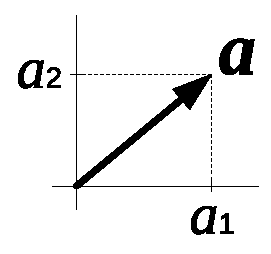
\includegraphics[keepaspectratio, width=3.1cm,height=3cm,clip]{chap9_ookisa001.pdf}
                \caption{2次元ベクトルの大きさ}
                \label{fig:chap9_ookisa001}
            \end{center}
        \end{figure}

        \subsection{基本演算}
        複数のベクトルがあるとき,ベクトル同士の演算を定義しておこう.
        ベクトルに対して定義される演算は,加算と減算と乗算であり,
        除算は定義されない.乗算には,
        定数倍,内積(スカラー積),外積(ベクトル積)の3種類がある.
        しかし,ここで言うベクトルの乗算は,
        普通の数で行われる乗算とは異なる概念であることに注意されたい
            \footnote{
                違いは,この後の説明で,自ずとわかるはず.
            }.
        ベクトルの演算が定義できるのは,すべてのベクトルの次元が同じ場合に限る.
        以下のベクトル演算の定義にでてくるベクトルは,すべて $n$ 次元
        ベクトルであると仮定する.次元が異なるベクトル同士の演算は定義しない.

        数学的な演算公理を示すことはせず,直感的にわかりやすい表現で
        演算の定義を示すにとどめておこう.

        \subsubsection{加算}
        2つの $n$ 次元ベクトル $\ba$,$\bb$ があるとき,
        この2つのベクトルに対する演算 $\ba+\bb$ を \textbf{加算} といい,
        次のように定義する.
        \begin{align}
            \ba + \bb   &:= (a_{1},\, a_{2},\,\cdots,\,a_{n}) + (b_{1},\,b_{2},\,\cdots,\, b_{n}) \notag \\
                        &=  (a_{1}+b_{1},\, a_{2}+b_{2},\,\cdots,\, a_{n}+b_{n} ).
        \end{align}

        成分を示す場合には,次のようになる.
        \begin{align}
            {(\ba+\bb)}_{i} := a_{i}+b_{i} \quad,\quad (i=1,\,2,\,\cdots,\,n).
        \end{align}
        添字の $i$ はベクトルの成分番号を示している記号である.式はすべての成分で
        成り立つが,すべての成分を書くと,上の定義のように,$i=1,\,2,\,\cdots,\,n$ の $n$ 通り
        を記述する必要が出てくる.しかし,どの成分番号に対しても,同じ形の式で
        定義で定義されることから,1から$n$の任意の一つを代表的に表す $i$ を導入した.

        \subsubsection{定数倍}
        スカラー $k$ と $n$ 次元ベクトル $\ba$ の積 $k\ba$ を \textbf{定数倍} といい,
        次で定義する.ここでは,$k$ を実数とする.
        \begin{align}
            k\ba := (k{a}_{1},\, k{a}_{2},\, \cdots,\, k{a}_{n}).
        \end{align}
        $\ba$ のすべての成分を $k$ 倍するということである.

        成分を示す場合には,次のように書く.
        \begin{align}
            {(k\ba)}_{i} := k{a}_{i} \quad,\quad  (i=1,\,2,\,\cdots,\,n).
        \end{align}

        \subsubsection{減算}
        加算と定数倍を定義しておけば,減算を定義する必要はない
            \footnote{
                一方に$-1$を乗じて(乗算)から,たし合わせればいい(加算).
            }.
        しかし,特徴的な演算であるため,この演算に \textbf{減算} という呼称を与える.
        減算は以下のような演算でのことをいう.2つの $n$ 次元ベクトル $\ba$,$\bb$ があるとき,
        ベクトルの減算 $\ba-\bb$ とは,
        \begin{align*}
            \ba-\bb &:= \ba + (-1)\bb \\
                    &= (a_{1}+(-1)b_{1},\, a_{2}+(-1)b_{2},\,\cdots,\, a_{n}+(-1)b_{n} ) \\
                    &= (a_{1}-b_{1},\, a_{2}-b_{2},\,\cdots,\, a_{n}-b_{n} )
        \end{align*}
        のような演算のことである.

        成分を示す場合には,次のようになる.
        \begin{align}
            {(\ba-\bb)}_{i} := a_{i}-b_{i} \quad,\quad (i=1,\,2,\,\cdots,\,n).
        \end{align}

        \subsubsection{内積(スカラー積)}
        2つの$n$次元ベクトル $\ba$,$\bb$ の内積 $\ba\cdot\bb$ とは,以下の演算のことをいう.
        \begin{align}\label{eq:chap9_naiseki001}
            \ba\cdot\bb := \sum_{i=1}^{n} a_{i}b_{i}.
        \end{align}

        展開したほうが,見やすいかもしれない(同じことを書いているだけ).
        \begin{align}
            \ba\cdot\bb := a_{1}b_{1} + a_{2}b_{2} + \cdots + a_{n}b_{n}.
        \end{align}

        演算結果がスカラーになることから,\textbf{スカラー積} ということもある.

        2次元ベクトルの場合,内積には図形的なイメージがある.
        それを強調した場合の,内積の定義は以下の通り.
        \begin{align}
            \ba\cdot\bb := |\ba||\bb| \cos \theta.
        \end{align}
        この定義は上の式(\ref{eq:chap9_naiseki001})の $n=2$ の場合と同値である.
        証明は後回し.
        \begin{figure}[htbp]
            \begin{center}
                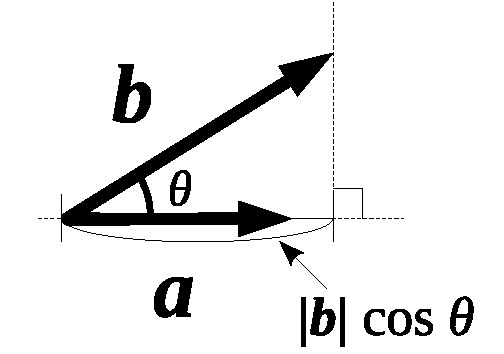
\includegraphics[keepaspectratio, width=4.23cm,height=3cm,clip]{chap9_naiseki001.pdf}
                \caption{内積}
                \label{fig:chap9_naiseki001}
            \end{center}
        \end{figure}

        \subsubsection{外積(ベクトル積)}
            \begin{mysmallsec}{外積の定義}
                2つの3次元ベクトル $\ba$,$\bb$ からなるベクトルの \textbf{外積} を
                $\ba\times\bb$ と表し,以下でその演算を定義する.
                    \begin{align*}
                            \ba \times \bb &:=& (\,
                                    a_{2}b_{3} - a_{3}b_{2},\;
                                    a_{3}b_{1} - a_{1}b_{3},\;
                                    a_{1}b_{2} - a_{2}b_{1}
                                \,)
                    \end{align*}

                演算結果がベクトルであることから,\textbf{ベクトル積} ということもある.

                唐突な定義で,無味乾燥だと思われるかもしれないが,
                根拠のあるものである.それを以下で説明しよう.
            \end{mysmallsec}

            \begin{mysmallsec}{一言}
                ベクトルの外積はわかりにくい.実際,定義式が少々複雑であり,図形的な
                イメージをすぐに描くには難しいかもしれない.しかし,ここを少々辛抱して
                手計算による練習をいくらかすることで,ベクトルの外積の意味やイメージを
                つかめるようになるはずである.
                ここでは,ベクトルの外積の定義を示すと共に,イメージを少しでも早くつかむ
                ことができるよう,丁寧に説明していく
            \end{mysmallsec}

            \begin{mysmallsec}{3次元ベクトルの外積のみを扱う}
                ここでの興味は3次元ベクトルの外積である.他の次元の外積は考えない.
                "興味がない"というのが直接的な理由だけれど,
                外積は内積のように簡単に $n$ 次元に拡張することができないことも,
                知っておいて損はないかも(多次元に拡張しようとして無駄な時間を費やさないように).

                外積の拡張に興味があれば,\textbf{外積代数} を学んでみる良い.
                外積代数は,ここでいう外積の自然な拡張ではないが(定義から違う),
                外積計算を発展させた形式の数学であることは実感できるだろう.
            \end{mysmallsec}

            \begin{mysmallsec}{定義の意味すること}
                ベクトルの外積とは,与えられた2つのベクトルから,
                この2つのベクトルの方向から独立した
                新しい方向を持つベクトルを1つ生成する演算である.
                その新しいベクトルの方向とは,2つのベクトルの両方に直交する方向であり,
                その大きさは $|\ba||\bb|\sin \theta$ である.
            \end{mysmallsec}

            \begin{mysmallsec}{外積の定義を知識0から作ろう}
                外積の定義の意味を実感するには,回り道かもしれないが,
                外積の定義に至るまでの思考プロセスをたどるとよい.
                先に示した外積の定義を一度忘れて,外積を1から作っていこう.
            \end{mysmallsec}

            \begin{mysmallsec}{外積の定義の目的}
                なぜ外積を定義したいのか.その理由は,外積を定義することにより,
                ある物理現象の数学的扱いが可能になるからである.必要は発明の母.
                力の釣り合いの解析には外積が欠かせないし,電磁気学ではローレンツ力
                を表すのに使われる.外積は闇雲に定義された演算ではなく,自然現象を
                詳細に観測した結果,それを説明するのに必要な演算方法なのである.
                自然現象の一部にはある特別な規則があり,それを数式で表そうとして
                試行錯誤して組み立てられた数学的概念が,外積なのである.
            \end{mysmallsec}

            \begin{mysmallsec}{外積演算に要求されること}
                2つの3次元ベクトル $\ba$,$\bb$ から,外積
                    \footnote{
                        今は,演算の名前なんてどうでも良い.知りたいのは
                        その具体的な演算方法である.この演算名は便宜的に
                        使用するものであり,"新しい演算方法"という
                        意味程度で捉えてもらいたい.
                    }
                によって生成したいベクトルの条件は以下の通りだった.
                \begin{enumerate}
                    \item 方向は $\ba$ と $\bb$ の両方に直交する方向である
                    \item 大きさは,$|\ba||\bb| \sin \theta$
                \end{enumerate}

                つまり,これから考えることは,
                \begin{enumerate}
                    \item 方向は 2つのベクトルに直交するようなベクトルをどう作るか.
                    \item さらに大きさを,$|\ba||\bb| \sin \theta$ にするには,どういう制約必要か
                \end{enumerate}
                の2点である.
                    \begin{figure}[hbt]
                        \begin{center}
                            \includegraphicslarge{gaiseki_01.pdf}
                            \caption{外積のイメージ}
                            \label{fig:gaiseki_01}
                        \end{center}
                    \end{figure}
            \end{mysmallsec}

            \begin{mysmallsec}{要求されることから,条件式を導く}
                2つの3次元ベクトル $\ba$,$\bb$ から,外積
                そのようなベクトルが仮に存在できたとして,それを $\bc$ と
                表すことにしよう($\bc:=\ba\times\bb$).

                $\bc$ は $\ba$ と $\bb$ の両方に直交しているから,内積が0になっているはずである
                    \footnote{
                        $\ba$,$\bb$ はともにゼロベクトルでないので(最初に要請される条件),
                        $|\ba| \neq 0$ ,$|\bb| \neq 0$ だから,$\cos(\pi/2)=0$ が
                        成立していなければならない.
                        $\ba$,$\bb$ の少なくとも一方がゼロベクトルである場合も外積は定義されるが,
                        この場合,新たに生成されるベクトルもゼロベクトルとなる特別な場合である.
                    }.

                したなら,次式が成立してなければならない.すなわち,
                    \begin{align*}
                        \ba \cdot \bc &= |\ba||\bc| \cos \frac{\pi}{2} = 0 \\
                        \bb \cdot \bc &= |\bb||\bc| \cos \frac{\pi}{2} = 0
                    \end{align*}
                である.
                ベクトル $\bc$ の成分を $(\,c_{1}\,,c_{2}\,,c_{3}\,)$ としよう.
                $\ba$ と $\bb$ についても同様に,
                それぞれ,$(\,a_{1}\,,a_{2}\,,a_{3}\,)$,
                $(\,b_{1}\,,b_{2}\,,b_{3}\,)$ とする.
                そうすると,上の2つの式は,また,以下のよう書いても同じことである.
                すなわち,
                    \begin{align*}
                        a_{1}c_{1} + a_{2}c_{2} + a_{3}c_{3} &= 0. \\
                        b_{1}c_{1} + b_{2}c_{2} + b_{3}c_{3} &= 0.
                    \end{align*}

                ベクトルの方向については,上の2式が成り立つことがその
                条件であるが,向きについては何も言っていない.
                そこで,次のように向きを決めてしまおう.すなわち,
                    \begin{description}
                        \item[向きの定義]
                            ベクトル $\ba$ とベクトル $\bb$ から生成する
                            外積 $\bc$ のむきは,
                            $\ba$ から $\bb$ に 向かって右ねじを右まわし回したときに,ネジが進む向きを,正方向とする.
                            これを満たすことを,\textbf{右手系をなす} という
                            別名「右ねじの法則」という表現が使われることも多い.
                    \end{description}

                    \begin{figure}[hbt]
                        \begin{center}
                            \includegraphicsdefault{migineji_01.pdf}
                            \caption{右ねじを回して進む方向}
                            \label{fig:migineji_01}
                        \end{center}
                    \end{figure}

                ベクトルにはもうひとつの性質である大きさ
                も考えないといけない.どのような大きさにしようと自由だが,
                最も簡潔に大きさを定めたい.もとの2つのベクトル $\ba$,$\bb$ より,
                この二つのベクトルが張る平行四辺形の面積を,その大きさと
                するのが最も簡単だろう.実際,数学的にもこのような定義が
                なされる.これが最も無理のない定義なのだろう.すると,
                $\bc$ の条件として,次式も加わることになる.
                    \begin{align*}
                        |\bc| &= | \ba || \bb | \sin\theta \\
                        &\Leftrightarrow \quad
                        \sqrt{{c_{1}}^{2}+{c_{2}}^{2}+{c_{3}}^{2}}
                        =
                        \sqrt{{a_{1}}^{2}+{a_{2}}^{2}+{a_{3}}^{2}}
                        \sqrt{{b_{1}}^{2}+{b_{2}}^{2}+{b_{3}}^{2}}
                        \sin\theta
                    \end{align*}

                これで,都合3つの条件式と,向きの定義は揃った.もう一度,まとめて書いておこう.
                \\
                \begin{itembox}[a]{外積演算で満たすべき条件式}
                    外積演算では,以下の条件式を満たさねばならない.
                    \begin{description}
                        \item[(1)] $a_{1}c_{1} + a_{2}c_{2} + a_{3}c_{3} = 0$ ($\bc \perp \ba$)
                        \item[(2)] $b_{1}c_{1} + b_{2}c_{2} + b_{3}c_{3} = 0$ ($\bc \perp \bb$)
                        \item[(3)] $\sqrt{{c_{1}}^{2}+{c_{2}}^{2}+{c_{3}}^{2}}
                               = \sqrt{{a_{1}}^{2}+{a_{2}}^{2}+{a_{3}}^{2}}
                                 \sqrt{{b_{1}}^{2}+{b_{2}}^{2}+{b_{3}}^{2}}
                                 \sin\theta$ (大きさ)
                        \item[(4)] $\ba,\,\bb,\,\bc$ は右手系をなす.(向き)
                    \end{description}
                \end{itembox}
                \\

                未知数が $c_{1}$,$c_{2}$,$c_{3}$ と三つなのに対し,
                条件式も同じく3つであり,数式的な条件としては必要十分である
                    \footnote{
                        これで,大きさと方向を定めることができる.
                    }.
                また,ベクトルの向きの定義もした.これで,外積を作る準備が
                整った.あとは,外積を作れるかどうか,言い換えれば,このように
                定義した外積というものが存在可能かどうかを,確認すれば良い.
            \end{mysmallsec}

            \begin{mysmallsec}{外積の成分表示}
                このような3式
                    \footnote{
                        正確には,「3つの式と,向きの定義」と書くべきだけど,
                        向きは人間が勝手に選ぶものなので,数式的に気にするもの
                        ではない.
                    }
                を満たすような $\bc$ は存在するのか.存在するとしたら,
                その成分はどのようになるか.それをこれから考えていこうと思う.それで,
                どうやって求めるかなんだけど,その方法は幾つか思い当たる.
                式をくどくどと計算をして発見的に答えを得る方法もあるけれど,
                それだと少々話が長くなり,計算も面倒くさい.なので,この問題の
                答えはすでに得られていることだから,先に答えを見てしまおう.
                そのほうが早い.

                で,その答えとは,
                    \begin{align*}
                        \bc &= (\,c_{1},\,c_{2},\,c_{3}\,) \\
                            &= (\,
                                    a_{2}b_{3} - a_{3}b_{2},\;
                                    a_{3}b_{1} - a_{1}b_{3},\;
                                    a_{1}b_{2} - a_{2}b_{1}
                                \,)
                    \end{align*}
                である.なにやら複雑な式に見えるが,次のように書くと,
                ある規則がみえてくるだろう.
                    \begin{align}\label{eq:VecGaiseki_Seibun}
                        \bc =
                        \left[
                            \begin{array}{c}
                                c_{1} \\
                                c_{2} \\
                                c_{3} \\
                            \end{array}
                        \right]
                        =
                        \left[
                            \begin{array}{c}
                                a_{2}b_{3} - a_{3}b_{2} \\
                                a_{3}b_{1} - a_{1}b_{3} \\
                                a_{1}b_{2} - a_{2}b_{1} \\
                            \end{array}
                        \right].
                    \end{align}

                $\ba$,$\bb$ の成分の添字を縦方向に意識して眺めると,
                巡回($1 \to 2 \to 3 \to 1$)しているのが見える
                    \footnote{
                        複雑そうに見えるけど,規則さえ分かってしまえば,
                        覚えるのはたやすい.最初の $a_{2}b_{3}$ さえ覚えてしまえば,
                        残りは機械的に記述できる.引く数は添字の数字を入れ替えた
                        ものだし,その他の成分については添字を巡回させればいい.
                    }.
                式(\ref{eq:VecGaiseki_Seibun})は,
                先ほど上げた3つの条件式を必要十分に満たす.
            \end{mysmallsec}

            \begin{mysmallsec}{外積の成分表示の検算}
                式(\ref{eq:VecGaiseki_Seibun})が本当に条件を満たすかどうかを,
                確かめておこう.まず,$\bc \perp \ba$,$\bc \perp \bb$ を
                満たすことを示す.やり方は,単純に条件式に成分を代入して,
                式を整理するだけである.

                条件式(1)について,
                    \begin{align*}
                         &a_{1}c_{1} + a_{2}c_{2} + a_{3}c_{3} \\
                         &\qquad=   a_{1}(a_{2}b_{3} - a_{3}b_{2})
                             + a_{2}(a_{3}b_{1} - a_{1}b_{3}) + a_{3}(a_{1}b_{2} - a_{2}b_{1}) \\
                         &\qquad=   a_{1}a_{2}b_{3} - a_{1}a_{3}b_{2}
                             + a_{2}a_{3}b_{1} - a_{2}a_{1}b_{3} + a_{3}a_{1}b_{2} - a_{3}a_{2}b_{1} \\
                         &\qquad= 0.
                    \end{align*}

                条件式(2)も同じように計算できる.
                    \begin{align*}
                         &b_{1}c_{1} + b_{2}c_{2} + b_{3}c_{3} \\
                         &\qquad=   b_{1}(a_{2}b_{3} - a_{3}b_{2})
                             + b_{2}(a_{3}b_{1} - a_{1}b_{3}) + b_{3}(a_{1}b_{2} - a_{2}b_{1}) \\
                         &\qquad=   b_{1}a_{2}b_{3} - b_{1}a_{3}b_{2}
                             + b_{2}a_{3}b_{1} - b_{2}a_{1}b_{3} + b_{3}a_{1}b_{2} - b_{3}a_{2}b_{1} \\
                         &\qquad= 0.
                    \end{align*}

                たしかに,二つの条件式を満たしている.このことにより,
                ベクトル $\bc$ は,ベクトル $\ba$,$\bb$ に直交している
                ことが確かめられた.つまり,ベクトル $\bc$ の方向は
                条件に沿うものであると言える.

                では,残りの大きさに関する条件式について,それを満たすか
                を計算してみよう.もう一度,大きさを決める条件式(3)を
                書くと,
                    \begin{align*}
                        &\sqrt{{c_{1}}^{2}+{c_{2}}^{2}+{c_{3}}^{2}}
                        =
                        \sqrt{{a_{1}}^{2}+{a_{2}}^{2}+{a_{3}}^{2}}
                        \sqrt{{b_{1}}^{2}+{b_{2}}^{2}+{b_{3}}^{2}}
                        \sin\theta
                    \end{align*}
                でるが,両辺を2乗して,
                    \begin{align*}
                        {c_{1}}^{2}+{c_{2}}^{2}+{c_{3}}^{2}
                        =
                        \left({a_{1}}^{2}+{a_{2}}^{2}+{a_{3}}^{2}\right)
                        \left({b_{1}}^{2}+{b_{2}}^{2}+{b_{3}}^{2}\right)
                        {\sin}^{2}\theta.
                    \end{align*}
                ここで,三角関数の公式 ${\sin}^{2}\theta + {\cos}^{2}\theta = 1$ を
                思い起こし,${\sin}^{2}\theta = 1 - {\cos}^{2}\theta $ と置き換えて,
                    \begin{align*}
                        &{c_{1}}^{2}+{c_{2}}^{2}+{c_{3}}^{2} \\
                        &\quad =    \left({a_{1}}^{2}+{a_{2}}^{2}+{a_{3}}^{2}\right)
                                    \left({b_{1}}^{2}+{b_{2}}^{2}+{b_{3}}^{2}\right)
                                    \left(1 - {\cos}^{2}\theta \right) \\
                        &\quad =    \left({a_{1}}^{2}+{a_{2}}^{2}+{a_{3}}^{2}\right)
                                    \left({b_{1}}^{2}+{b_{2}}^{2}+{b_{3}}^{2}\right) \\
                                    &\quad \qquad -\left({a_{1}}^{2}+{a_{2}}^{2}+{a_{3}}^{2}\right)
                                        \left({b_{1}}^{2}+{b_{2}}^{2}+{b_{3}}^{2}\right)
                                        {\cos}^{2}\theta.
                    \end{align*}
                最後の行の
                    \begin{equation*}
                        \left({a_{1}}^{2}+{a_{2}}^{2}+{a_{3}}^{2}\right)
                        \left({b_{1}}^{2}+{b_{2}}^{2}+{b_{3}}^{2}\right)
                        {\cos}^{2}\theta.
                    \end{equation*}
                に注目すると,
                    \begin{align*}
                        &\left(
                            \sqrt{{a_{1}}^{2}+{a_{2}}^{2}+{a_{3}}^{2}}
                            \sqrt{{b_{1}}^{2}+{b_{2}}^{2}+{b_{3}}^{2}}
                            {\cos}\theta
                        \right)^{2} \\
                            &\qquad=
                            \left(
                                \ba \cdot \bb
                            \right)^{2} \\
                            &\qquad=
                            \left(
                                a_{1}b_{1}+a_{2}b_{2}+a_{3}b_{3}
                            \right)^{2}.
                    \end{align*}

                つまり,大きさの定義式は以下のように書き換えられる.
                    \begin{align*}
                        &{c_{1}}^{2}+{c_{2}}^{2}+{c_{3}}^{2} \\
                        &\qquad =   \left({a_{1}}^{2}+{a_{2}}^{2}+{a_{3}}^{2}\right)
                                    \left({b_{1}}^{2}+{b_{2}}^{2}+{b_{3}}^{2}\right)
                                    \left(1 - {\cos}^{2}\theta \right) \\
                        &\qquad =   \left({a_{1}}^{2}+{a_{2}}^{2}+{a_{3}}^{2}\right)
                                    \left({b_{1}}^{2}+{b_{2}}^{2}+{b_{3}}^{2}\right)
                                    -   \left(
                                            a_{1}b_{1}+a_{2}b_{2}+a_{3}b_{3}
                                        \right)^{2}.
                    \end{align*}

                この式を,ベクトル $\bc$ が満たしていることを確認すればよい.
                    \begin{align*}
                        |\bc|^{2}
                        &=
                        {c_{1}}^{2}+{c_{2}}^{2}+{c_{3}}^{2} \\
                        &=
                         {(a_{2}b_{3} - a_{3}b_{2})}^{2}
                         + {(a_{3}b_{1} - a_{1}b_{3})}^{2}
                         + {(a_{1}b_{2} - a_{2}b_{1})}^{2} \\
                        &=
                        \left(
                            {a_{2}}^{2}{b_{3}}^{2} + {a_{3}}^{2}{b_{2}}^{2} - 2a_{2}a_{3}b_{2}b_{3}
                        \right)
                        + \left(
                            {a_{3}}^{2}{b_{1}}^{2} + {a_{1}}^{2}{b_{3}}^{2} - 2a_{1}a_{3}b_{1}b_{3}
                        \right) \\ &\qquad
                        + \left(
                            {a_{1}}^{2}{b_{2}}^{2} + {a_{2}}^{2}{b_{1}}^{2} - 2a_{1}a_{2}b_{1}b_{2}
                        \right) \\
                        &=
                          {a_{2}}^{2}{b_{3}}^{2} + {a_{3}}^{2}{b_{2}}^{2} + {a_{3}}^{2}{b_{1}}^{2}
                        + {a_{1}}^{2}{b_{3}}^{2} + {a_{1}}^{2}{b_{2}}^{2} + {a_{2}}^{2}{b_{1}}^{2} \\
                        &\quad - 2a_{2}a_{3}b_{2}b_{3} - 2a_{1}a_{3}b_{1}b_{3} - 2a_{1}a_{2}b_{1}b_{2} \\
                        &=
                          \left({a_{1}}^{2}{b_{3}}^{2} + {a_{1}}^{2}{b_{2}}^{2}\right)
                        + \left({a_{2}}^{2}{b_{3}}^{2} + {a_{2}}^{2}{b_{1}}^{2}\right)
                        + \left({a_{3}}^{2}{b_{2}}^{2} + {a_{3}}^{2}{b_{1}}^{2}\right) \\
                        &\quad - 2a_{2}a_{3}b_{2}b_{3} - 2a_{1}a_{3}b_{1}b_{3} - 2a_{1}a_{2}b_{1}b_{2}.
                    \end{align*}

                ちょっと一息.まだまだ式変形は続く.ちなみに,上式の冗長な括弧は,
                以降の式変形のために,明示的に記述している.

                次に,トリッキーな作業をする.それは,ある数 $x$ に対して,
                当然,$0=x-x$ が成り立つから,0を加えるということは $x-x$ を加えることと同じである.
                そして0を加えても等式は成り立つ.
                この考え方を利用して,式変形を続けよう.
                    \begin{align*}
                        |\bc|^{2}
                        &= {a_{1}}^{2}{b_{3}}^{2} + {a_{1}}^{2}{b_{2}}^{2}
                            + \left({a_{1}}^{2}{b_{1}}^{2} - {a_{1}}^{2}{b_{1}}^{2}\right) \\
                        &\quad + {a_{2}}^{2}{b_{3}}^{2} + {a_{2}}^{2}{b_{1}}^{2}
                            + \left({a_{2}}^{2}{b_{2}}^{2} - {a_{2}}^{2}{b_{2}}^{2}\right) \\
                        &\quad + {a_{3}}^{2}{b_{2}}^{2} + {a_{3}}^{2}{b_{1}}^{2}
                            + \left({a_{3}}^{2}{b_{3}}^{2} - {a_{3}}^{2}{b_{3}}^{2}\right) \\
                        &\quad - 2a_{2}a_{3}b_{2}b_{3} - 2a_{1}a_{3}b_{1}b_{3} - 2a_{1}a_{2}b_{1}b_{2} \\
                        &=   {a_{1}}^{2}\left({b_{1}}^{2} + {b_{2}}^{2} + {b_{3}}^{2}\right)
                           + {a_{2}}^{2}\left({b_{1}}^{2} + {b_{2}}^{2} + {b_{3}}^{2}\right)
                           + {a_{3}}^{2}\left({b_{1}}^{2} + {b_{2}}^{2} + {b_{3}}^{2}\right) \\
                        &\quad -{a_{1}}^{2}{b_{1}}^{2} - {a_{2}}^{2}{b_{2}}^{2} - {a_{3}}^{2}{b_{3}}^{2}
                               - 2a_{2}a_{3}b_{2}b_{3} - 2a_{1}a_{3}b_{1}b_{3} - 2a_{1}a_{2}b_{1}b_{2} \\
                        &=  \left( {a_{1}}^{2} + {a_{2}}^{2} + {a_{3}}^{2} \right)
                            \left( {b_{1}}^{2} + {b_{2}}^{2} + {b_{3}}^{2} \right)
                           -\left(a_{1}b_{1}+a_{2}b_{2}+a_{3}b_{3}\right)^{2}.
                    \end{align*}

                式変形が長々と続いたが,これでやっと確かめられた
                \footnote{
                    以下の恒等式が成立している.
                        \begin{equation*}
                            \left( X + Y + Z \right)^{2}
                            = {x}^{2} + {y}^{2} + {z}^{2} + 2XY + 2YZ + 2ZX.
                        \end{equation*}
                    ここでは,$X=a_{1}b_{1}$,$Y=a_{2}b_{2}$,$Z=a_{3}b_{3}$ に対応している.
                }.

                条件式(4)は,条件式(1)(2)(3)では特定することのできなかった向きを
                人為的に定めるものである.うるさいことを言うと,条件式(4)が条件式(1)(2)(3)に
                矛盾しないことを示すべきだが,割愛する.どちらの向きを正とするか,という問題
                であり,大げさに議論するところではない.単なる取り決めである.

                以上から,$\bc$ は3つの条件式を満たすことが確かめられ,ベクトルの外積が
                存在することが示された.つまり,ベクトルの外積は定義可能であることが確かめられた.
            \end{mysmallsec}

            \begin{mysmallsec}{最後に一言}
                何度も言うが,ベクトルの外積は導かれるものではない.人の想像力によって
                定義するものである.この外積という概念を導入することで,物体の回転を数学的に
                扱うことができるのである.というか,実際は話が逆で,ベクトルの外積の定義に従う
                物理現象が発見され,この現象を数学的に扱うことができるように,外積が定義される
                のである.もしかしたら,外積の定義が突拍子も無いと感じているかも知れないが,
                現実に外積を用いて説明される物理現象が生じているのである.外積はその現象を
                扱うために導入されるのだ.
            \end{mysmallsec}

                \begin{memo}{右手系とは何か}
                    外積の定義のうちの,向きの定義をもう一回読んでみよう.

                    \begin{description}
                        \item[向きの定義]
                            ベクトル $\ba$ とベクトル $\bb$ から生成する
                            外積 $\bc$ のむきは,
                            $\ba$ から $\bb$ に 向かって右ねじを右まわし回したときに,ネジが進む向きを,
                            正方向とする.これを満たすことを,\textbf{右手系をなす} という.
                    \end{description}


                    なぜこのように定義するのかという疑問があろうが,この疑問
                    はすぐに捨て去るべきだ.なにしろ,答えがないのだから.
                    しかし,天下り的な説明はよくない.なので,できるだけ
                    “もっともらしい”説明を,以下に記述しておくことにしよう
                        \footnote{
                            あくまでも,“もっともらしく”記述するのであり,
                            これがほんとうの理由だとか,正解だとかというものではない.
                            天下り的な説明ではスッキリとせず,モヤモヤしてしまう
                            ので,これを少しでも解消できればと考えて,記述
                            するものである.
                        }.

                    2つのベクトル $\ba$,$\bb$ に直交する方向は内積の数式で表現され,
                    数学的に議論できるが,方向は計算で導くことはできない.なので,
                    予め,向きを定めておくのである.どちらの向きを正方向としても,
                    それ以降で変更しなければ,論理に矛盾は生じない.しかし,向きを
                    決めないと議論ができないので,人為的な向きの定義を施すのである.

                    では,なぜ,「右ネジをまわして進む向き」と表現するのか.
                    これにも,多分,明確な答えはない.
                    おそらく,これが最も簡潔な言い回しで,誤解なく,加えて直感的イメージ
                    しやすく説明できるからだろう.しかし,学術的には格好をつけて,
                    「右手系をなす」と言われる.それは,右手の親指を人差し指に近づけるという
                    行為が,親指を右まわしするという行為に当たり,中指の先の向きが
                    外積の向きに一致するからである.元となる2つのベクトルが親指と人差し指に
                    値し,それに直交する向きに中指が向いているのだ.
                    \begin{figure}[hbt]
                        \begin{tabular}{cc}
                            \begin{minipage}{0.5\hsize}
                                \begin{center}
                                    
\includegraphics[keepaspectratio, width=3cm,height=3.75cm,clip]{migitekei_TE_2.pdf}

                                    (a) 右手
                                    \label{fig:migitekei_TE_mono_x}
                                \end{center}
                            \end{minipage}
                            \begin{minipage}{0.5\hsize}
                                \begin{center}
                                    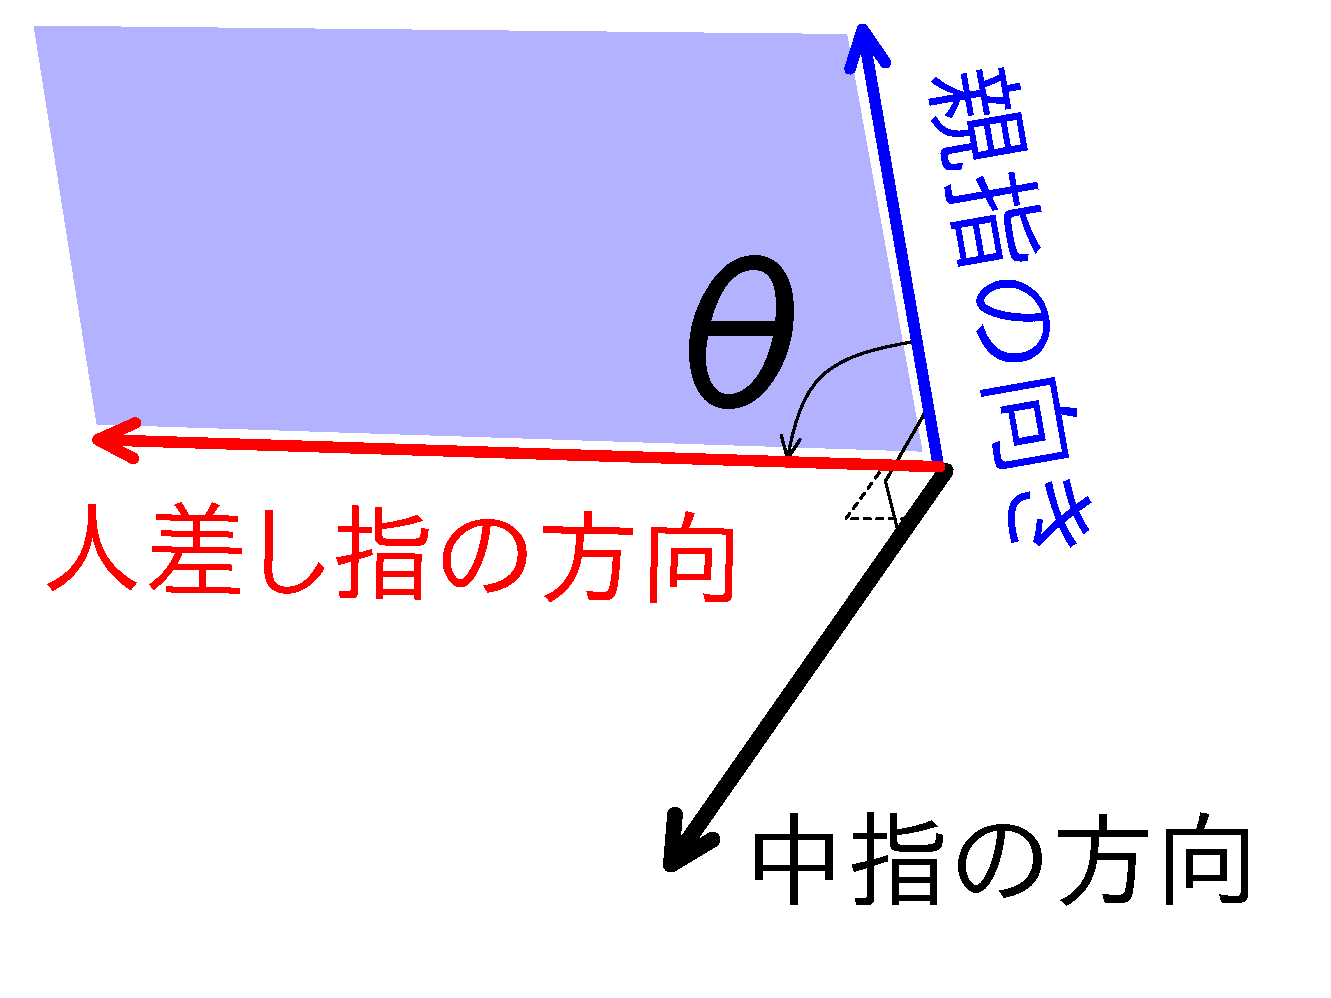
\includegraphics[keepaspectratio, width=3cm,height=3.75cm,clip]{migineji_Myhand.pdf}

                                    (b) 対応図
                                    \label{fig:migineji_Myhand}
                                \end{center}
                            \end{minipage}
                        \end{tabular}
                        \caption{右手系}
                    \end{figure}
                \end{memo}

        \subsubsection{乗算?}
            ベクトルの乗算を,加算と同じように定義できないだろうか.
            つまり,2つの $n$ 次元ベクトル $\ba=(a_{1},\,a_{2},\,\cdots,\,n)$,
            $\bb=(b_{1},\,b_{2},\,\cdots,\,n)$ を用いて,
                \begin{equation*}
                    {(\ba \ast \bb)}_{i} = a_{i}b_{i}
                \end{equation*}
            と定義してはだめか
                \footnote{
                    記号に $\ast$ を使った理由は,内積の記号に $\cdot$,
                    外積の記号に $\times$ が使われるため,これらと区別
                    したかったためである.
                }.
            先人がこのように定義をしていないからには,
            できない理由があるに違いない.しかし,このように
            乗算を定義しても,不整合が起きるわけでもなく,定義不可能
            とは思えず,むしろ定義可能であると思えて仕方ない.
            私の力では,この定義を採用しない強い理由を見つけられない.

            しかし,このような乗算を定義してしまうと,ベクトルと数の違いが全く
            なくなってしまうことは確かだ
                \footnote{
                    実際に試してみてほしい.数と全く同じで,ベクトルを
                    定義した意味が全く感じられないことだろう.
                }.
            つまり,ベクトルとは表記上の利便性が向上
            しただけで,数学的な新しい概念となるわけではなくなる.
            数学的な発展を考えた場合,このような仕方の冗談の定義では
            前進がないので無駄ということになる.要するに,こんな乗算を定義
            してしまっては,わざわざベクトルを定義したことが無意味になって
            しまうのだ.表記方法を工夫しただけで新しい数学的概念とは言えない.
            もちろんこれでは,物理学にとっても,何のご利益もない
            ものになってしまうことだろう.
            だから,むしろ意識的に,このような定義を避けているのではない
            かと思われる(確証はない).ベクトルに内積や外積を定義することで,
            物理学に有用な数学になると共に,とても興味深い数学的対象となる.

        \subsubsection{除算??}
            ベクトルの内積の定義を採用すると,
            ベクトルの除算を定義することは難しい,と悟るのは容易だろう
            \footnote{
                $\bX\cdot\ba=k$ のとき,単純に $\ba=k/\bX$ とはできそうにない.
                $\bX$ をベクトルの変数とみなしたときに,この式を満たす $\bX$ は
                無限に存在するするから,できるとするならば,何か条件や約束事が必要だが,
                いい案は思い当たりそうにない.例えば,無限に存在する解をひとまとめにして,
                "解空間"(微分方程式など解空間とはべつもの)なるものをでっち上げたとしても,
                これ以上の発展は見込めないだろう.
            }.

            上記の "$\ast$" 乗算が採用されるのであれば,同じように除算を
            定義することは可能である.それは単に数を並べただけなので,
            吸うと全く同じ四則演算を定義すれば,不整合は起こらない.
            上記の乗算を定義しない理由に従うと,内積や外積を定義した方が
            学問的に有益である.そうなると,除算の定義が格段に難しくなる,
            というか,定義できたとしても条件が複雑すぎて,つまらなくなるだけだろう.

            だから,除算が定義できないのではなく,学問的に有益でないから定義しない
            と言ったほうが,正確なのであろう.

            数における0除算の禁止も,数学的に有益ではないから定義しないのだ,言えなくもない.
            よく挙げられる0除算が禁止される理由として,それを仮定すると不整合が起きるからだ
            といった説明がなされることがある
                \footnote{
                     $a$ を任意の数とするとき,$a \cdot 0 = 0$ が成立する(0の存在公理).
                     このとき,$a \neq b$ なる $b$ をもってきても $b \cdot 0 = 0$ である.
                     よって,$a \cdot 0 = b \cdot 0$(ここまでは正しい).
                     \textbf{両辺を0で割ると} $a=b$ となるが,これは $b$ の最初の条件に
                     矛盾する(不整合の発生).よって,0除算は禁止とされる.
                }.
            しかし,これは決して論理的な説明でない(美しい言い訳ではあるけれど).
            不整合が起きないように定義しなおせばよい.
            数学の論理は自然に存在するものではなく,人間が勝手気ままに構築
            するものであるから,定義なんていくらでも好き勝手できるはずである.ただ,
            0除算が定義できるようなうまい約束事を見つけられたとしても,複雑怪奇な理論
            が出来上がることになるのだろう(そんな理論に誰が興味を持つだろうか).

        \subsection{分解}
        1つのベクトルを複数のベクトルに分割することも可能である.
        例えば,$\ba = \bb + \bc$ が 成立しているとき,
        ベクトル $\ba$ は 2つのベクトル$\bb$と$\bc$に分割可能である.
        等式が成立していれば,分割するベクトルの個数に際限はない.
        このように,1つのベクトルを,加算が成り立つように複数のベクトルに
        分割することを,ベクトルの \textbf{分解} という.

        \subsection{単位ベクトル}
        大きさが1のベクトルを \textbf{単位ベクトル} という.
        単位ベクトルの記号は教科書により様々である.
        このノートでは,$\bn$ を単位ベクトルの記号として使用する
        \footnote{
            ただし,常にこの記号を用いるわけではない.その場合は,その直前か直後
            に説明を書くこととする.
        }.

        定義から,以下が成立する($n$ 次元を想定).
        \begin{align}
            |\bn| = \sqrt{\sum_{n=1}^{n} {n_{i}}^{2}} = 1.
        \end{align}
        $n_{i}$ のそれぞれの値には興味はないが,上記の関係式を満たす.
        単位ベクトルの方向は問わない.

                \subsection{演算の諸性質(公式)}
        \begin{mycomment}
            ベクトル基本的な演算性質を記しておく.
            $\ba$,$\bb$,$\bc$,$\bd$ はベクトルで,$k$,$l$ はスカラーである.
            括弧の内部の計算は,それがない部分よりも,優先度が高い(先に計算すべき)とし,
            それ以外の計算は左から順に計算する.
        \end{mycomment}

        \subsubsection{加算と定数倍に関する公式}
            ベクトルの加算と定数倍に関する演算性質は,スカラーの場合と変わらない.
            代表的な演算を以下に書いておく.
            \begin{enumerate}
                \item $\ba + \bb = \bb + \ba$
                \item $(\ba + \bb ) +\bc = \ba + (\bb + \bc)$
                \item $k (\ba + \bb) = k\ba + k\bb$
                \item $k(l\ba) = l(k\ba) =(kl)\ba$
                \item $\ba = \ba + \bzero = \bzero + \ba$
                \item $\ba +(-1)\ba = \bzero$
                \item $1\ba = \ba$
            \end{enumerate}

            以下,簡単に説明を与えておく.
            \begin{enumerate}
                \item 項の順序を入れ替えてから加算しても,結果は変わらない.\textbf{交換法則} とよばれる.
                \item 加算の順番を入れ替えても,結果は変わらない.\textbf{結合法則} とよばれる.
                \item 加算と定数倍に関する性質.
                      加算してから定数倍しても,両者を定数倍してから加算しても,どちらも
                      同じ結果になる.\textbf{分配法則} とよばれる.
                \item スカラーのかける順番を変えても,結果はわらなない.
                \item ゼロベクトル $\bzero$ を足しても結果は変わらない.
                      法則ではなく,$\bzero$ の存在を認めるもの.
                \item ベクトルから自身を引くとゼロベクトルになる.
                      $(-1)\ba$ は $\ba$ の \textbf{逆ベクトル} という.
                      $\ba$ も $(-1)\ba$ の逆ベクトルである(逆ベクトルの一意性).
                \item スカラーの1倍の1は記述を省略できる.
            \end{enumerate}

            どれも,定義から丁寧に計算すれば自明であるので,証明するまでもない
            \footnote{
                本音は$\cdots$
                \begin{itemize}
                    \item "記述が面倒だから省略させてほしい" という甘え
                    \item "書いたところで,ノートの記述が煩雑になって読みにくくなる" という言い訳
                    \item "自分で計算すれば,理解の確認になるのではないか" という逃げ
                \end{itemize}
                である.

                証明するには,式の両辺を独立に成分計算し,
                対応する成分同士が等しいことを確認すればいい.
                一意性を示したい場合には,異なる2つのものがあると仮定しても,
                両者が同値になることを示せばいい.
            }.

        \subsubsection{内積に関する公式}
            内積もスカラーと同じように扱える.主な性質は以下の通り.
            \begin{enumerate}
                \item $\ba \cdot \ba = {|\ba|}^{2}$
                \item $\ba \cdot \bb = \bb \cdot \ba$
                \item $\ba \cdot (\bb + \bc) = \ba \cdot \bb + \ba \cdot \bc$
                \item $(\ba + \bb) \cdot \bc = \ba \cdot \bc + \bb \cdot \bc$
                \item $k(\ba \cdot \bb) = (k\ba) \cdot \bb = \ba \cdot (k\bb)$
                \item $\ba \parallel \bb \Leftrightarrow \ba \cdot \bb = 0$
                \item $\ba \perp \bb \Leftrightarrow \ba \cdot \bb = \displaystyle\frac{\pi}{2}$
            \end{enumerate}

            言葉でも説明しておこう.
            \begin{enumerate}
                \item 自身の内積は,自身の大きさの2乗に等しい.
                \item 内積の項の順序を入れ替えても,結果は変わらない.
                \item 分配法則が成り立つ
                \item 分配法則の別の形(1と2より自明だろう)
                \item 定数倍と内積に関して,結合法則が成り立つ.
                \item 2つのベクトルが平行であることと,それらの内積が0であることは等価
                \item 2つのベクトルが垂直であることと,それらの内積が$\displaystyle\frac{\pi}{2}$であることは等価
            \end{enumerate}

            \begin{mysmallsec}{内積の使い所}
                物理学でベクトルの内積を使う場合は,2つのベクトルの交わりの角度を気にする場合が
                ほとんどである.平行なのか,垂直なのか,そうでなければどんな角度で交わっているのかが,
                内積の計算によってわかるからである.
            \end{mysmallsec}

        \subsubsection{外積に関する公式}
            外積の演算性質は,他とは異なるので,注意が必要である.
            \begin{enumerate}
                \item $\ba \times \ba = \bzero$
                \item $\ba \times \bb = - \bb \times \ba$
                \item $\ba \times (\bb \times \bc) = (\ba \cdot \bc) \bb - (\ba \cdot \bb) \bc $
            \end{enumerate}

            簡単にコメントを書いておく.
            \begin{enumerate}
                \item 自身の外積はゼロベクトルである.
                \item 外積の項の順序入れ替えると,符号が反転する.
                \item \textbf{ベクトルの三重積} という異名をもつ.
                      ちなみに,右辺の $\ba \cdot \bc$,$\ba \cdot \bb$ の演算結果はスカラーである.
            \end{enumerate}

            他にもたくさんあるけど,省略する.ベクトルの外積に関する公式は,
            一見して複雑な形をしたものが多く(検算が大変),挫折しがちだ.
            しばらく見ていると規則性が見えてきて,美しく感じるのかもしれないが,
            頻繁に使うのは上の3つくらいだ.後は,必要になったらときに,公式集を参照しよう.

        \subsubsection{単位ベクトルに関する公式}
        任意のベクトルは,同じ向きの単位ベクトルの定数倍である
            \footnote{
                証明はしないけど.
            }.
        アタリマエのことを言っているようだが,確認しておこう.
        ある $n$ 次元ベクトルを用意して,$\bX$ としよう.
        単位ベクトルの向きは,$\bX$ と同じとする.
        $\bX$ を単位ベクトル $\bn$ の定数 $k$ 倍と表せたとすると,$\bX = k\bn$ と
        なる.$\bX=(X_{1},\,X_{2},\,\cdots)$,$\bn=(n_{1},\,n_{2},\,\cdots,\,n)$ とすると,
            \begin{equation*}
                X_{i} = kn_{i} \quad,\quad (i=1,\,2,\,\cdots,\,n)
            \end{equation*}
        が成り立つ.これを踏まえて,$\bX$ の大きさ $|\bX|$を考えてみよう.
        簡単な計算で,$|\bX|=k$ が導ける.
            \begin{equation*}
                |\bX| = \sqrt{\sum_{n=1}^{n} {X_{i}}^{2}}
                      = \sqrt{\sum_{n=1}^{n} {(kn_{i})}^{2}}
                      = k \left(\sqrt{\sum_{n=1}^{n} {n_{i}}^{2}}\,\right)
                      = k \cdot 1
                      = k.
            \end{equation*}
        ここで,単位ベクトルの大きさが1であることを使用した.

        以上から,任意のベクトルは単位ベクトルを自身の大きさで定数倍したものに等しい,と言える.
        式で書くと,次の通り.
        \begin{align}
            \bX = |\bX|\bn.
        \end{align}

        上式を逆手に考えて,
        \begin{align}
            \bn = \frac{\bX}{|\bX|}= \frac{1}{|\bX|} \bX.
        \end{align}
        と見ることで,任意のベクトルの単位ベクトルを計算することもできる.

        しかし,次は無意味であることに注意しておくこと.
        \begin{align*}
            \mbox{(意味のない式)}\quad|\bX| = \frac{\bX}{\bn}
        \end{align*}
        ベクトル同士の除算は定義されておらず,この式は何も意味しない.


%%%        %======================================================================
%  Chapter : ベクトル解析
%  説明    : 電磁気学を記述する上で必要なベクトル解析のまとめ
%======================================================================

%======================================================================
%  Section
%======================================================================
    \section{ベクトル解析}
    \subsection{ベクトル変数(あるいは,変数ベクトル)}
    ベクトルには,スカラーにおける語彙「変数」に対応する,一般的呼称がない.
    ないと不便なので,このノートでは \textbf{ベクトル変数} という言い方を導入する.
    もしかしたら,\textbf{変数ベクトル} と書くこともあるかもしれない.

    細かいことを言うと,ベクトル変数は,
    成分の一部あるは全部が変数であるようなベクトルであり,
    次に説明するベクトル関数である
        \footnote{
            定義が論理的に循環してしまっているが,意図は伝わるはず.
            循環しないような記述も可能だが,理論構築が目的ではない
            ため,深く突っ込まないでおこう.
        }.

    変数をベクトル変数と区別する意味で,\textbf{スカラー変数} と
    書くこともある.

    \subsection{ベクトル関数}
    ベクトルが絡む関数のことを総称して \textbf{ベクトル関数} という.
    また,ベクトル関数と区別するために,
    今まで考えてきたベクトルが絡まないような関数を,
    \textbf{スカラー関数} と表現する場合がある
        \footnote{
            細かいことを言うと,スカラーは1次元ベクトルだから,
            スカラー関数もベクトル関数である.
        }.

    考えれる例をいくつか上げておこう.特にこれらを区別してよぶ必要は
    ないので,名称を与えることはしない
        \footnote{
            記述の際には,どんな形の
            ベクトル関数について議論している
            かが明確にわかるようにする.
        }.

    例えば,スカラーの独立変数 $t$ に対して,
    1つの定ベクトルが定まる関数が考えられる.これを
        \begin{align}
            \ba (t)
        \end{align}
    と表す.
    関数記号 $\ba$ を太字にした意図は,
    ベクトルが定まる(値域がベクトルである)ことを明示するためである.
    また,$(t)$ という表記は,$t$ が独立変数であることを示すものである
        \footnote{
            多変数になる場合,$\ba(t,\,s)$ と書かれることになる
            ($t$ と $s$ はスカラーである).
            このとき,$(t,\,s)$ という記述がベクトルを成分表示と同じで,
            紛らわしいかもしれない.しかし,文脈により容易に区別できる
            とし,特に書き分けることはしない.この記述の前に関数を
            表現する文字があれば,それらは独立変数である.
        }.

    別の例を上げると,ベクトル変数を独立変数にもつ関数が考えられる.
    数式で表そうとすると,
        \begin{align}
            \ba (\br)
        \end{align}
    のようになる.$\br$ はベクトル変数である.

    上記2つの混合して,スカラー変数 $t$ とベクトル変数 $\br$ から
        \begin{align}
            \ba (t,\,\br)
        \end{align}
    という関数を作ってもいい.

    ベクトル変数を独立変数として,スカラーが定まる(値域がスカラーである)
    関数もあり得る.記号化すれば,
        \begin{align}
            a (\br)
        \end{align}
    となるだろう.関数記号 $a$ を細字にした意図は,スカラーが定まることを
    明示するためである.

    もちろん,スカラー変数 $t$ とベクトル変数 $\br$ をもち,
    スカラーが定まる関数も考えられる.
        \begin{align}
            a (t,\,\br)
        \end{align}

    定ベクトルもベクトル関数の一部として考える.
    明示的な独立変数はないが,入力にかかわらず常に一定値をとるような
    関数として捉える.スカラー関数の場合と同じように考える.

    独立変数が1つのベクトル関数($\ba(t)$)を,\textbf{1変数ベクトル関数} という.
    独立変数が2つ以上のベクトル関数を総称して,\textbf{多変数ベクトル関数} という.
    ベクトル変数をもつベクトル関数($\ba(\br)$ など)は多変数ベクトル関数として考える.

    ひと目で見やすいように,表にしておこう(\Table\ref{table:f4unit}).
        \begin{table}[htb]
          \centering
          \caption{ベクトル関数の種類}
          \begin{tabular}{|l|c|c|l|}                                        \hline
            関数記号      & 独立変数   & 値域     & 例                      \\ \hline  \hline
            $\ba$         & なし       & ベクトル & 定ベクトル              \\ \hline
            $\ba(t)$      & $t$        & ベクトル & ある1点の風向の時間推移 \\ \hline
            $\ba(\br)$    & $\br$      & ベクトル & ある時刻の風向分布      \\ \hline
            $\ba(t, \br)$ & $t$,$\br$ & ベクトル & 風向分布の時間推移      \\ \hline
            $a(\br)$      & $\br$      & スカラー & 風力分布                \\ \hline
            $a(t, \br)$   & $t$,$\br$ & スカラー & 風力分布の時間推移      \\ \hline
          \end{tabular}
          \label{table:f4unit}
        \end{table}

    \subsection{ベクトル関数の微積分}
    \begin{mycomment}
        スカラー関数での微積分を,ベクトル関数へ拡張する.
        ベクトル関数の微積分も,基本的にはスカラー関数と同じように
        計算可能である.
    \end{mycomment}

    \subsubsection{極限}
    ベクトル関数の極限はスカラー関数の場合と同じように定義できる.

    \subsubsection{導関数}






%%%
%===================================================================================================
%  Chapter : 電磁気学が対象とする現象
%  説明    : 電磁気学の対象となる,電気的現象・磁気的現象の実在についての確認をする
%===================================================================================================
\chapter{電磁気学が対象とする現象}
%   %-----------------------------------------------------------------------------------------------
%   %  Input
%   %    File Name : PhysNote_EM_1st_Intro.tex
%   %    説明      : 電磁気学を構成する基本的な概念を説明する.
%   %-----------------------------------------------------------------------------------------------
        %===================================================================================================
%  Chapter : 電磁気学が対象とする物理現象
%  説明    : 電磁気学の対象となる,電気的現象・磁気的現象の実在についての確認をする
%===================================================================================================

%======================================================================
%  Section
%======================================================================
    \section{はじめに}\label{sec:EM_ObjPreMsg}
        \begin{mycomment}
            本節では,以降の電磁気学への導入と,これからの電磁気学の
            学習の段取りを説明する.
        \end{mycomment}

    %======================================================================
    %  SubSection
    %======================================================================
    \subsection{電気と磁気}\label{subsec:ElcAndMgn}
        これから学習する電磁気学は,\textbf{電気} と \textbf{磁気} が起こす
        様々な現象を説明する物理学の分野の1つである.
        電気とか磁気とかというと,日常的に用いられている使い慣れた言葉であり,
        そのイメージも多くの人々が共有している.「何を今更」と思われるかもしれないが,
        今まで日常的に使われてきた「電気」とか「磁気」とか
        という言葉と,そのイメージを一度整理しておきたい.
        これから学習する電磁気学は,電気とは何か,あるいは,磁気とは何かを
        探求するものであり,その疑問となる根本的な現象についてを確認せずに
        話を進めるには,甚だ滑稽なことだろう.

    %======================================================================
    %  SubSection
    %======================================================================
    \subsection{電気と磁気の伝わり方}%\label{subsec:ElcAndMgn}
        私達の感じてる電気や磁気は,実際には,静電気の引力
        (あるいは斥力)というように,力として現れている.つまり,力の伝達の
        表現方法が必要になってくる.
        “力の伝達”と聞いて,なんのことだ? と思ったかもしれない.
        というのも,ニュートン力学では,力の伝播については無視していたからである.
        そこでは,暗黙の了解として,「力は瞬間的に,つまり,時間0で伝わる」
        ということが仮定されていたのだ.しかし,このような考え方では,無限に遠くに存在する
        物体にも,近隣に存在する物体にも,力が "同時" に伝わる事になってしまう.
        これは直感に反するのではないだろうか.近くにある物体には,すぐに力が
        伝わり,遠くにあるものほど力の伝わり方が遅いというように,
        力の伝播に時間がかかるとしたほうが,自然な考え方では
        なかろうか.まあ,何れにしても,実験的に確かめないといけないところ
        だが,現在では,一般相対性理論で説明されるとおり,力の伝播には,時間
        がかかることがわかっている.つまり,力が一瞬で伝わると仮定されている
        ニュートン力学は,この部分において,間違っている.その間違いの修正は
        追々やっていくとして,ここでは,力の伝播をどうやって式で表現できるか
        を考えないといけない.
        そこで,力の伝播を表現するための概念である,\textbf{場} という考え方が
        導入される
            \footnote{
                小言を言っておこう.

                「場」という考え方は自然な考え方であるが,概念が抽象的すぎて,
                なかなか初学者にとって受け入れ難いことだろう.
                しかし,我慢して欲しい.「場」という考え方は,これからいっそう重要に
                なってくる.現代の物理学は,「場」という考え方が理論構築の基礎になっているからである.
                はじめに「場」ありき,という考えが一般的なのだ.
                理由はわからないが,そういう考え方のもとで,理論構築をし,成功を収めている.

                この部分は,"自然だけども特殊な考え方"なので,
                最初学習する上でつっかえる所だろう.理解するのに,
                時間がかかってしまうが,悩まずに,学習を進めていってもらいたい.
                数式とそのイメージをリンクさせようともがきながら
                (いろいろ考えたり,ヒントとなる本,Webサイトを探したりしよう)
                学習を進めれば,いつの間にか,「場」という考え方に慣れて
                (毒されて?)しまうものである.

                こんなことをここで言うな,と言われるかもしれない.実際そのとおりで,
                あとでまた同じ事を言うことだろう.ここでは,“この先に困難がありますよ”
                という案内として記述したまでである.
                (RPG風に言うなら,「(王様の台詞) 勇者よ,お前はこれから多くの困難に直面
                することだろう.しかし,それに屈してはならない.どんな困難だろうとも,
                それに立ち向かい,解決せねばならない.いかなる困難も克服し,壮大な目標に
                向かって,前進するのだ.行け,勇者よ,そして,いつの日か目的を果たし,
                帰還するのだ.」といった感じだ.)
            }.

    %======================================================================
    %  SubSection
    %======================================================================
    \subsection{電気・磁気の研究の歴史(ダイジェスト)}
        電磁気学で着目する力は,\textbf{電磁気力} と言われる.これは,
        \textbf{電気的な力} と \textbf{磁気的な力} の両方を指す言い方
        である.電気的な力や磁気的な力の存在自体は,摩擦時に起こる静電
        気や磁石の存在から,古くから知られていたことだろう.
        しかし,その力の持つ性質を科学的に扱うことができるのは,16世紀
        になってからである.ギルバート
            \footnote{
                William Gilbert(1544--1603, イギリス):Gilberd と
                表現されることもある.電磁気現象を近代的な実験方法で
                研究した,最初の人物のひとりとして有名である.検電器
                を発明している.医者としての仕事の傍ら,電磁気の研究
                をしていたらしい.
            }
        による電磁気現象の研究が,電磁気学の幕開けとするのが通説のようである.
        しかし,より正確に電磁気現象が扱えるようになるのは,
        キャベンディッシュ
            \footnote{
                Henry Cavendish(1731--1810, イギリス):化学と物理学
                の研究で有名.人間嫌いであったり,研究した結果を秘密
                にしておいたりと,特異な性格を強調されることが紹介さ
                れる言が多い(あ,ここにも書いてしまった).地球の
                比重を測定したことでも有名.これにより,万有引力の存
                在の裏付け,並びに,地球の重力定数の測定がなされた.
                また,電磁気学に関して言えば,クーロンの法則をクーロ
                ンよりも前に発見したことが,キャベンディッシュ死後に,
                マクスウェル(※1)より明らかにされている.

                (※1)James Clerk Maxwell(1831--1879, イギリス).
                \ref{subseq:4fundlaw_Hajimeni}節の脚注を参照.
            }
        やクーロンが電気的な力のもつ性質を実験的に解析する18世紀ごろである.
        アンペール
            \footnote{
                Andre-Marie Amp\'{e}re(1775--1836, フランス):電流に関
                する実験で有名.電流の単位「アンペア[A]」は彼の名にちなん
                だものである.
            }
        による電流と力の関係
            \footnote{
                この関係は,アンペールの法則と言われる.詳しいことは,後述する.
            }
        の発見や,ビオ
            \footnote{
                Jean-Baptiste Biot(1774--1862, フランス):物理学者であり,
                数学者,天文学者でもある.後に述べる,ビオ$=$サバールの法則
                の発見者のひとりとして有名.大気圧の測定も行っていたらしい.
            }
        とサバール
            \footnote{
                F\'{e}lix Savart(1791--1841, フランス):ビオと共同で,
                ビオ$=$サバールの法則を提唱したことで有名.カタカナ表記では,
                「サヴァール」と書いたほうが,正確なのかもしれない(だけど,
                このノートでは「サバール」と書くことにしたい.こっちのほうが
                見慣れたカタカナので,つっかえることなく読めると思う).
                外科医でもあったらしい.また,現在の音程の単位はセント(1
                オクターブ$=$1200セント)であるが,それ以前の単位として,
                サバール(savart)が使われていた.ちなみに,音程1サバールは
                だいたい4セントくらいである(なので,だいたい1オクターブは
                300サバールということになるのか).
            }
        の磁気と電流の関係の研究もだいたい19世紀初期に行われていている.最終的な
        電磁気学の確立がマクスウェルによってなされるのが19世紀中頃(1864年)である.

        電磁気現象は古くから知られていたのに対し,その現象を科学的に
        扱えるようになるのは,19世紀中頃になってからであった.そもそも科学という
        考え方自体が,ルネッサンス期に芽生えたものとされているので,仕方がないの
        かもしれないが,それにしても,電磁気現象を人間が把握するのに,これだけの時間が
        かかっているのには驚きである
            \footnote{
                話がそれるが,今日ある私たちの生活環境は,
                パソコンや携帯電話など,電磁気学を応用して作り
                出されている.そう,私たちの掌の中には,それだけの
                研究の重さがのしかかっているのである.ただ持っているだけでは
                なんにも感じないけど,少し学習すると,それらの機器を見たとき,
                先人の研究努力に対し,感謝の気持ちを懐くことだろう.
            }

%======================================================================
%  Section
%======================================================================
    \section{電気的現象}
        世の中には,接触していないにもかかわらず,力を受けることがある.
        この非接触で感じる力の中に,\textbf{電気的な力} がそのひとつとして
        存在する.

        例えば,髪の毛を下敷きでこすり,その後すぐに下敷きを頭の上の方へゆっ
        くりと持ち上げてみると,髪の毛は下敷きに吸いつけられるかのように持ち
        上がる.この現象を,一度は,小学生のころに実験や遊びで経験したことと思う.
        \textbf{電気的現象} の一例として,頻繁に頻繁にあげれる現象だ.
        この現象を物理学的には電磁気学で説明される.
        特に,静電気学として語られることが多い.
        静電気学は,電磁気学でも最も基本となる考え方である.
        になる.

%======================================================================
%  Section
%======================================================================
    \section{磁気的現象}
        非接触的に受ける力の別の例として,\textbf{磁気的な現象} も考えられる.
        鉄などの特定の金属をひきつける
            \footnote{
                ひきつける:相対的に考えれば,「引き寄せられる」といっても同
                じこと.
            }
        石がこの世界には存在し,日本では \textbf{磁石} と呼ばれている.これ
        は電気的な現象とは異なる原因から生じる.この磁気的な現象についても,
        後ほど詳しく考えることになる.

%======================================================================
%  Section
%======================================================================
    \section{電磁気的現象}
        電気的現象と磁気的現象は,その発生原因は異なるのだが,それらの振
        る舞いはとても似ている部分が多い.このことから,電気的現象と磁気的現
        象は密接な関係があるが容易に想像され,実際にあとで示す通り,
        この予想は正しい.
        両者を共に扱う場合,これらの現象をひっくるめて,\textbf{電磁気的現象} と
        よぶ.

        電磁気的現象の例として,\textbf{電磁波} という,物理現象がある
            \footnote{
                そして,これの例に尽きる.
            }.
        携帯電話や無線LANに代用される無線通信機器は,この電磁波を利用している.

        第一段階の電磁気学の学習目標は,電磁気的現象を数式で表現することである.


    \begin{memo}{非接触的な力}
        物体に触れることなしに与える力を,非接触的な力という.
        非接触的な力は磁石などでも馴染みがあり,馴染みのある現象
        だ.しかし,よく考えてみると,不思議な現象だ.
        触っていないのに力が伝わるのである.このような現象を見て,
        どのようにこの力の伝達を説明できるだろうか.
        私達の直感では,物体に触れていないのに力が伝わるということを理解し難い.
        しかし,現実に磁石は存在して,非接触的な力が目の前で起こっている.
        どうしたことだろうか.物理学者はこの不可解な非接触的な力を説明すべく,
        \textbf{場} という概念を発案した
            \footnote{
                英語で言うと,Fieldである.
            }.
        物体が力を受けるということの原因はその周囲の場の歪みであると解釈せよ,
        というのである.

        いきなり場という考え方を提示され,わけわからん状態に陥ってるかもしれない.
        しかし,安心してほしい.場という概念は,誰にとっても,言葉で説明されただけでは理解し難いものだ
            \footnote{
                物理の教科書を書いている偉い先生も,場という概念を理解するのに
                苦労した経験があるそうだ.
            }.
        これからの物理学の学習(演習)を続けることで,言葉だけでなく,感覚的にも
        理解できるようになるだろう
            \footnote{
                場という概念は非常に抽象的(数学的)であり,実際にその存在を示すことはできない.
                だから理解し難いし,初めのうちは胡散臭く感じるのだが,学習を進めることでそれなしでは
                物理学を構築に欠かせない概念であることを悟るだろう.
            }.
    \end{memo}





%===================================================================================================
%  Chapter : 電磁気現象の根源
%  説明    : 電荷の存在や,電流の存在などを確認する
%===================================================================================================
\chapter{電荷 --- 電磁気現象の根源 ---}
%   %-----------------------------------------------------------------------------------------------
%   %  Input
%   %    File Name : PhysNote_EM_1st_GeneralIdea.tex
%   %    説明      : 電荷と電流の概念を確認する.
%   %-----------------------------------------------------------------------------------------------
        %===================================================================================================
%  Chapter : 電磁気学の基本概念
%  説明    : 電荷の存在や,電流の存在などを確認する
%===================================================================================================

%======================================================================
%  Section
%======================================================================
\section{電荷}
    %==================================================================
    %  SubSection
    %==================================================================
    \subsection{電荷の存在}
    \begin{mysmallsec}{電磁気現象の根源は電荷である}
    電磁気学を構築するにあたり,最も重要な要請がある.
    それは,\textbf{電荷の存在} だ.電荷はすべての電磁気現象の根源である.
    電荷には,\textbf{正の電荷} と \textbf{負の電荷} の2種類が存在する.
    電気のもつ2つの性質,すなわち,
    "引きつける力(\textbf{吸引力})"と"反発する力(\textbf{反発力})"を
    説明するために,導入される概念である
        \footnote{
            これは観測事実であり,他から導かれる現象ではない.
            電気的現象を注意深く観察した結果,電気には吸引力と反発力の2種類
            があることがわかったのだ.なぜ第3の性質がないのか,という疑問は却下される.
            電磁気学にとって,電荷の存在の要請こそが理論の土台であり,その存在理由は問わない.
            もしかしたら,後の物理学の進展により明らかになるのかもしれないが,
            少なくとも電磁気学で説明されることではない.
        }.
    正の電荷を「プラス($+$)の電荷」,負の電荷を,「マイナス($-$)の電荷」ということもある.
    図で表現する場合,$+$ や $-$ で表されることが多い.このノートでも,これに従う.

    電気現象や磁気現象を説明するためには,電荷という概念を受け入れないと
    ならない.ここで言う電荷の存在は,仮定なのだが,この仮定を受け入
    れることにより,電磁気現象を説明できる.存在するかどうかも
    わからない概念を受け入れるのには,少々躊躇してしまうことではあるけれ
    ど,そこをこらえて \textbf{電荷というものが存在する} と認めてもらいた
    い.
    \end{mysmallsec}

    \begin{mysmallsec}{電磁気学の理論体系に電子は不要}
    電荷というと,現在では,電子の存在が当たり前のように知られているが,
    電磁気学が成立した時代には,電子は知られていなかった.電子は電磁気
    学が成立した後に,電磁気学自身の理論を基にした実験により,発見され
    た経緯がある.だから,電子という概念は,電磁気学の理論体系では,表
    面にはでてこない.電子の発見以前に電荷という概念が確立しており,電
    磁気学は,この電荷を基礎に組み立てられた理論なのである.よって,電
    磁気学を学ぶ上で,電子の知識は不要である.これからしばらくの間は,
    電子という概念をしばらく忘れ,正電荷と負電荷の2種類の電荷が存在する
    として,話を進めていく.
    \end{mysmallsec}

    \begin{mysmallsec}{吸引力と反発力のイメージ}
    電荷が存在するという仮定の最も基本的な実験法則に,\textbf{クーロンの法則} と
    いうものがある.電気は反発したり,引き付け合ったりするという性
    質を主張する法則である.後で詳しく触れることにしよう.
        \begin{figure}[hbt]
            \begin{center}
                \includegraphicslarge{EM_Denka_No_Katei.pdf}
                \caption{電気現象と2種類の電荷}
                \label{fig:EM_Denka_No_Katei}
            \end{center}
        \end{figure}

    とにかく,ここでは,「電荷が存在すると電磁気現象をうまく説明できる」
    ということを理解してもらいたい.
    \end{mysmallsec}

    \begin{mysmallsec}{電荷を表すのに使う記号($Q$,$q$)}
    電荷を記号で表すときには,$Q$ や $q$ が使われることが多い
        \footnote{
            $Q$ や $q$:電磁気学の内容を記述する場合には,説明なしに暗黙
            の了解として使用されることもある.物理では,式に現れる文字の
            意味を常に意識しておくことも大事だ.
        }.
    ただし,これは後に説明する電気量についての意味も含まれている.
    \end{mysmallsec}

    %==================================================================
    %  SubSection
    %==================================================================
    \subsection{電荷は2種類しかないのか}
    なぜ電荷は2種類しかないと言えるのだろうか.もしかしたら,未発見
    の第3の電荷
        \footnote{
            「正」でも「負」でもない,電荷の働きをするもの.いや,3
            つでなくとも,4,5,6,…と,もっと種類が存在しもよいの
            ではないか.
        }
    は実在しているかもしれない,という可能性があるではないか.確かに,
    この可能性は完全に否定する事はできない.実際,見つかっていない第
    3の電荷を“仮定”し,理論を組み立てるできるだろう.しかし,物理
    学の教科書には,「電荷は2種類である」としか書かれていない.なぜ
    か.これは,理論には単純性が追求されるからである.

    確かに,3種類以上の電荷があると仮定しても理論は組み立てられるかもしれない
        \footnote{
            検討したことはない...
        }.
    しかしたとえ可能であったとしても,その場合,
    電荷が2種類であるという仮定してつくられた理論
    よりも,説明に要する仮定が多くなってしまうだろう.理論はより単純な方が
    採用される
        \footnote{
            単純な理論は1つとは限らないだろう.同じ程度,単純な理論
            をつくることは,不可能ではないと思う.
            実際,重力を含む統一理論の構築段階で,ループ量子重力理論と超弦理論の
            2つが提案されている.

        }.
    電磁気の理論を組み立てるのには,最小数でも2種類の電荷が必要であり,2つの
    電荷を仮定すると,電磁気現象が全て
        \footnote{
            “全て”とは,言い過ぎかもしれない.未発見の現象がある可
            能性が否定できないからだ.しかし,電磁気学の歴史は長く,
            実験も多くなされていてるので,おそらく,理論が覆されるよ
            うな電磁気的実験結果は得られないだろう.
        }
    導出できる.さらに,3つ以上の電荷が存在すると仮定した場合の理論
    よりも,2種類のみの電荷を仮定した理論の方が,単純である.こうし
    たことから,電荷は2種類だというのである.

    物理学は,論理学や数学とは違い,科学である.科学は実験結果が全て
    であるので,論理的に矛盾がなくても,実験結果が理論と異なれば,その理論
    は間違いである
        \footnote{
            ただし,その実験は,本当に正しいことを確かめないといけな
            い.
        }.
    電磁気学にも,理論と異なる実験結果が得られてしまう恐れがあるかも
    しれない.科学に絶対はありえない.しかし,今までに,「実験も理論
    もともに一致して,不一致になったことはない」ということから,電磁
    気学は“科学思想的に”正しい理論であると言える.

    %==================================================================
    %  SubSection
    %==================================================================
    \subsection{荷電粒子,点電荷}
    電荷を帯びた粒子のことを,\textbf{荷電粒子} とよぶ.
    ニュートン力学において,物質を数学的に扱いやすくするために質点という
    概念を導入した.質点とは,質量をもつ点のことであった.電磁気学でもこ
    れと同じように,\textbf{点電荷} というものを定義する.点電荷とは,電
    荷をもつ点のことである.荷電粒子を理想化して,その大きさを無視できる
    程に小さくしたものとも考えてもよい.とにかく,点電荷とは,大きさのな
    い電荷をもつものと捕らえてもらいたい.ただ,質点も点であるが質量をも
    つのと同じく,点電荷にも質量はある.
        \begin{figure}[hbt]
            \begin{center}
                \includegraphicslarge{EM_Denka_Tendenka.pdf}
                \caption{点電荷(イメージ)}
                \label{fig:EM_Denka_Tendenka}
            \end{center}
        \end{figure}

    荷電粒子や点電荷を記号で表現するときには,$q$ が用いられることが多い.


    %==================================================================
    %  SubSection
    %==================================================================
    \subsection{電荷は実際に存在するか}
    あたりまえのことだが,電荷は目で見ることができない
        \footnote{
            見ようとしても,見ることは不可能である.どんなに高性能な顕微
            鏡を開発したとしても,“電荷そのもの”を見ることは不可能であ
            る.この理由は,量子力学で説明されよう.
        }.
    だから,電荷を直接“肉眼(あるいは顕微鏡)で”確認することは不可能であ
    る.しかし,見えないのだから存在しない,と考えてはならない.電荷の存
    在を考えなければ,説明できない現象が山ほどあるのだ
        \footnote{
            いや,逆だった.現象を説明するために,「電荷」とい う概念を
            導入したのであった.
        }.

    実は,電磁気学を駆使した実験によって,電荷の存在を実証できる(検電器など).
    だけど,
    その実験を理解するには電磁気学の知識が必要である.話が堂々巡りになっ
    ていると感じるかもしれないが,そうではない.電磁気学ではあくまでも,
    電荷の存在は仮定されているだけものに過ぎない.しかし,電磁気学の知識
    を活用した実験により,電荷の存在を確証するに値する実験結果を得るので
    ある.
        \begin{figure}[hbt]
            \begin{center}
                \includegraphicslarge{kendenki_fix.pdf}
                \caption{検電器}
                \label{fig:kendenki}
            \end{center}
        \end{figure}

    \begin{memo}{電子の存在と電磁気学}
            荷電粒子は,電磁気現象を説明するために,人間が作り出した仮説
            に過ぎなかったが,後にこの荷電粒子が実在されることが,実験的
            に示された.この実在する荷電粒子のことを,今日我々は \textbf{電子} と
            よんでいる
                \footnote{
                    電子: 「でんし」と読む.「でんこ」ではないよ.
                }.

            電子の存在はトムソン
                \footnote{
                    Joseph John Thomson (1856竏驤1940, イギリス)
                }
            によって発見された.電子の発見は1897年であり,マクスウェルによる電磁気学
            の成立は1873年である.つまり,電子の発見よりも電磁気学の成立のほうが
            早かったのである.

            要するに,電磁気学は,電子の存在を認めて作られたものではない.あくま
            でも,“電荷”を基礎にして,電磁気学は構成されるのである.だから,電
            磁気学を学んでいく上で,その例として出てくる電子は単なる仮想粒子に過
            ぎない.存在するかしないかわからないような,粒子なのである.

            むしろ,確立された電磁気学によって,電子の存在が認められたのである.
            電磁気学を学ぶ上では,電子の存在はあまり気にする必要はない.というこ
            とで,電子についての詳細は,原子論を学習するときに改めて考える.ここで学習すべきは電磁気学なのだから.
        \end{memo}

    %==================================================================
    %  SubSection
    %==================================================================
    \subsection{電気量}
    電荷のもつ電気を定量的に扱う場合,これを数値として表さないといけない.
    \textbf{電気量} とは,電荷のもつ電気を定量化したものである.電気量の
    単位は,「クーロン[C]」が用いられる.この単位は物理学者クーロン
        \footnote{
            Charles-Augustin de Coulomb(1736--1806, フランス):クーロン
            の法則の発見者として,その名が知られている.電磁気に関する研究
            が多い.
        }
    に因んで名づけられている.1[C]の定義(仮)は,以下の通り
        \footnote{
            1[C]の定義(仮):(仮)と書いたのは,現在の国際標準の単位系
            であるSI単位系による定義ではないためである.この1[C]の定義は,
            このノートでは,後ほどSI単位系に則した定義に改める.しかし,
            この定義を述べるには,ある程度の電磁気の知識が必要であり(
            SI単位系は電磁気学の確立後に制定された),ここで述べることは
            できない.だけど,1[C]を無視して話を進めることは難しいので,
            ここでは便宜的にこの仮の定義を採用している.
        }.
    \\
    \begin{itembox}[l]{\textbf{1[C]の定義(仮)}}
        同じ電気量をもつ点電荷を2個用意する.この2つの点電荷を1[m]だけ離し
        て固定したとき,この点電荷に$8.99 \times 10^{9}$[N]の力が働くとき,
        この両点電荷のもつ電気量を1[C]とする.
    \end{itembox}
    \\

    なぜこのような定義としているのかという疑問が浮かぶはずだが,これについ
    ては「クーロンの法則」のところで明らかになるだろう.ここでは,とりあえ
    ず認めてほしい.

    %==================================================================
    %  SubSection
    %==================================================================
    \subsection{電気素量}
        電荷について,面白いことが分かっている.
        \textbf{電荷には最小値が決まっている}のである.
        つまり,現実世界に存在する電気量は,
        \textbf{最小値の整数倍でしか存在していない} ということだ.

        重要な事実なので,何度も繰り返す.
        電気量には最小値が存在し,この最小値を $e$ と表す.
        さらにこの時,この世界に実在する電気量は,最小値 $e$ の
        整数 $n$ 倍で存在する.$(1/2)e$ とか $(5/3)e$ なんていう
        電気量は存在しないのである.現実に存在しているのは,
        $2e$ とか $5e$ のように,最小単位 $e$ の整数倍なのだ.

        次のように言っても良い.
        \textbf{電気量にはこれ以上分割でない最小の単位が存在する}.
        この電気量の最小値 $e$ を,\textbf{電気素量} という.

        電気素量 $e$ の具体的な値は,今日ではSI単位系で,
            \begin{align}
                e=1.602177 \times 10^{-19} [\mathrm{C}]
            \end{align}
        とされている.この数値は実験によって得た数値である.
        また,単位系のとり方により,その数値は異なるので注意
            \footnote{
                (参考)1987年までの電気素量の値は
                    \begin{equation*}
                        e=1.60217733(49)\times 10^{-19} [\mathrm{C}]
                    \end{equation*}
                 とされている.
            }.

        以降では,電気量 $q$(あるいは $Q$)という表現を頻繁に使用する.
        電気量 $q$ は電気素量の整数倍でしか存在し得ないので,
        その整数を $n$ とした時に,$q=ne$ と表せる.
        しかし,電気素量の概念は,電磁気学の理論構築には,不要である
            \footnote{
                電気素量の発見は,電磁気学が体系化された後でなされている.
                電気素量の存在理由もわかっていない.
            }.
        むしろ,電荷の存在自体が重要であり,電磁気学の主役となる量は電気量 $q$ である.
        電気量 $q$ を,電気素量 $e$ を用いて詳しく書けば,$ne$ となるのだが($n$ は整数),
        こう表しても式が煩雑になるだけなので,以降の記述は電気量 $q$ という
        表現を使うことにする
            \footnote{
                ここからしばらくは,巨視的な(目で見える大きさという意味で)電磁気現象
                を念頭に置いて,電磁気学を学習する.つまり,電気素量が数えきれないくらい
                たくさんある(整数 $n$ がとても大きい)場合を中心に考えることになる.
                この場合は,電気素量は考える必要がない.

                ただし,電気素量という概念が重要でないということではない.電磁気学成立後に発見
                された電子の運動を定量的に考える場合には,電気素量が重要になる.
                電子1つの運動のような,目に見えないくらい微視的なな世界を考える場合には,
                電気素量という考え方が重要になってくる.ただ,ここでは巨視的な電磁気現象が
                メインなので,電気素量という概念を使う必要がないだけ,ということ.
            }.

        \begin{memo}{電気素量をどう見つけたか}
            驚くことに,電気素量の発見,つまり,電子の発見は,電磁気学の成立以後である.
            それまでは,上に書いたように,電荷は仮想的なものに過ぎなかった.電子の発見は,
            電荷という概念をより確かなものにした.

            ちょっとまてよ.“電荷そのもの”を見ることはできないと,上に書いたではないか.
            うそをついたのか.いや確かに,“電荷そのもの”を見ることはできない.では,なぜ
            電荷を発見したと言えるのか.それは,\textbf{トムソンの陰極線} の発見で説明される
            .この実験で,電荷が,電子として実在することを示した.でも,具体的に,どれくらい
            の電荷量をもつかは,トムソンの発見からは,分からなかった.電子の電荷量,つまり,
            電気素量は,ミリカンによる油滴の実験により,明らかになった.
                \begin{figure}[hbt]
                    \begin{center}
                        \includegraphicslarge{denkisoryou_fix.pdf}
                        \caption{油滴実験}
                        \label{fig:denkisoryou}
                    \end{center}
                \end{figure}

            おもしろい話だ.電子の発見は,電磁気学の理論を利用した実験によって発見された,といういことになる.
            電荷の存在を仮定した電磁気学によって,電子が発見されたのだ.
            何か,一見して矛盾してそうな気がする.
            電磁気現象の根源である電荷が,電荷を仮定した電磁気学を用いて,発見されたからだ.
            しかし,少し考えれば,これは矛盾ではない.
            電磁気学は電荷が実在しなくとも,成立しているのである.もちろん,
            電荷が存在しないことが発見されてしまったら,それは理論と実験で矛盾が起こる.
            だけど実際は,電荷が電子として実在することが分かった.だから,矛盾ではない.
            むしろ,理論と実験の整合性が高まったのだ.
        \end{memo}

    %==================================================================
    %  SubSection
    %==================================================================
    \subsection{電荷密度}
    非常に多くの点電荷が集まっている状況を考える.このとき,個々の点電荷
    を区別して考えるよりも,点電荷の集まりそのものを扱うほうが賢明な場合
    も多い.このとき,点電荷の集まり具合のことを \textbf{電荷密度} とよぶ.
        \begin{figure}[hbt]
            \begin{center}
                \includegraphicslarge{EM_DenkaMitudo.pdf}
                \caption{電荷密度(イメージ)}
                \label{fig:EM_DenkaMitudo}
            \end{center}
        \end{figure}

    電荷密度を記号で表すときには,$\rho$ で表すことが多い
        \footnote{
            この記号 $\rho$(「ロー」と読む)は,電気回路を扱う場合,
            抵抗率として用いられる.$\rho$ が電磁気学で現れたら,何の
            断りもなければ,電荷密度であると考えてよいだろう.ただし,
            電気回路で $\rho$ が現れたら,何を意味しているのかを注意し
            た方がよい.とりあえず,このノートの電磁気学の部分では,
            $\rho$ は電荷密度としての意味で用いる.
        }.
    特に,位置に
    よって電荷密度の値が異なるときには,位置ベクトル $\br$ を用いて,
    $\rho(\br)$ と書かれる.

    \begin{memo}{電荷密度の表現上の問題}
        電荷密度 $\rho(\br)$ は多数の電子が存在し,その個数を把握することが
        現実問題として難しく,その必要もない場合に大いに役に立つ.
        現実世界では,この状況のほうが一般的である.

        しかし,何か怪しい部分がある.それは,電荷密度が位置 $\br$ の
        関数として書かれていることにある.一点には広がりなんてものは考え
        られない.つまり,面積が0なので,面積で割ることができず,密度
        が定義できないのである.
        0で割ることは無限大になることを意味している.
        この問題を同処理すればよいか.いや,上手いこと回避する方法が
        あるのか.実は,この無限大の電荷密度を回避する方法がある.
        それは,ディラックの \textbf{デルタ関数} $\delta(\br)$ である.
        このディラックのデルタ関数は後ほど述べる
            \footnote{
                \pageref{subsub:delta_function}ページの
                \ref{subsub:delta_function}節を参照.
            }.
    \end{memo}

    %==================================================================
    %  SubSection
    %==================================================================
    \subsection{電荷密度と全電気量の関係}
    系の全電気量 $Q$ と電荷密度 $\rho(\br)$ の関係を示しておこう.

    系の全電気量が分かっている場合,その全電気量を $Q$ とする.
    電荷密度 $\rho(\br)$ が存在している所に,微小な体積 $\df V$ をとる
    (図\ref{fig:EM_DenkamdV}).この微小体積 $\df V$ の内側の
    電気量を $\df Q$ と書こう.このとき,
        \begin{align*}
            \df Q = \rho(\br)\df V
        \end{align*}
    当関係が成立している
        \footnote{
            次元的にも,
            \begin{align*}
                [\mathrm{C}] = [\mathrm{(Cm^{-3})\cdot m^{3}}]
            \end{align*}
            が成立している.
        }.
    全電気量 $Q$ はこの式の両辺を積分すれば良い.
    積分の範囲は,電荷密度が存在しているすべての領域に
    対して行う.これは体積分
        \footnote{
            「体積積分」といわれることもある.
        }
    と呼ばれる計算である.
        \begin{align}
            \vint \df Q &= \vint \rho(\br)\df V \notag \\
            \therefore \quad
                     Q &= \vint \rho(\br)\df V
        \end{align}

    もし,任意の閉曲線 $S$ の内側の領域 $\OmegaS$ にある
    電気量 $Q_{\OmegaS}$ を計算したい場合は,積分範囲をこの領域にすればよいだけである.
        \begin{align}
            \vint_{\OmegaS} \df Q &= \vint_{\OmegaS} \rho(\br)\df V \notag \\
            \therefore \quad
                     Q_{\OmegaS} &= \vint_{\OmegaS} \rho(\br)\df V
        \end{align}

    まとめておこう.
        \begin{myshadebox}{電荷密度と全電気量の関係}
            閉曲面 $S$ の内側の領域を $\OmegaS$ と表記する.
            $\OmegaS$ 内に存在する全電気量 $Q_{\OmegaS}$ と
            電荷密度 $\rho(\br)$ には次の関係がある.
            \begin{align}
                Q_{\OmegaS} = \vint_{\OmegaS} \rho(\br)\df V
            \end{align}
            ここに,$\df V$ は微小体積を表す.
        \end{myshadebox}

        \begin{figure}[hbt]
            \begin{center}
                \includegraphicslarge{EM_DenkamdV.pdf}
                \caption{電荷密度と全電気量}
                \label{fig:EM_DenkamdV}
            \end{center}
        \end{figure}

    \begin{memo}{微小体積}
        微小体積とは,全体積のうちの微小な一部分のことである.
        \begin{figure}[hbt]
            \begin{center}
                \includegraphicslarge{EM_smollV.pdf}
                \caption{微小体積}
                \label{fig:EM_smollV}
            \end{center}
        \end{figure}
    \end{memo}

    \begin{memo}{体積分の表示方法}
        体積分は,3方向にわたる積分である.
        つまり,2つの積分変数 $u$,$v$,$w$ を
        考えたとき,これを変数に持つ関数 $f(u,\,v,\,w)$ をとし,
            \begin{equation*}
                \int \left(
                    \int \left(
                        \int f(u,\,v,\,w) \df u
                    \right)  \df v
                \right) \df w
            \end{equation*}
        を計算することが,体積分を行うということである.

        つまり,$f(u,\,v,\,w)$ を最初に $u$ について積分して,
        その結果を $v$ について積分し,
        さらにその結果を $w$ について積分する
        ということである.計算方法を示すには,このような
        表示の仕方が有効であるが,この表現からでは体積分であることをイメージする
        には,少々難しい.そこで,式を次ように書き換えてみる.
            \begin{equation*}
                 \vint f(u,\,v) \df u \df v \df w
            \end{equation*}
        括弧をなくしただけである.そして,
        $\df V := \df u\df v \df w$ という量を導入し,
        さらに,3回の積分を改て $\vint_{V}$ と表現することで,
            \begin{equation*}
                \vint_{V} f(u,\,v,\,w) \df V
            \end{equation*}
        となる.これならば,体積 $V$ で体積分するというイメージが
        しやすい式の表現になった.

        ちなみに,$\df V := \df u\df v\df w$ は \textbf{体積素} とよばれる.
    \end{memo}


    %==================================================================
    %  SubSection
    %==================================================================
    \subsection{$\delta$ 関数}\label{subsub:delta_function}
        %==================================================================
        %  SubsubSection
        %==================================================================
        \subsubsection{$\delta$ 関数の定義}\label{subsub:delta_function_teigi}
            電気量 $q$ をもつ1つの点電荷の電荷密度 $\rho(\br)$ を表すことを考える.
            点電荷の位置を $\br_{0}$ とする.このとき, $\br_{0}$ を内部に含む領域 $\Omega$ で
            体積積分すると,全電荷量 $q$ をしめす.つまり,
                \begin{align}
                    q=\int_\Omega\rho(\br)\df V \quad,\quad \left( \br_{0} \in \Omega \right)
                \end{align}
            と書ける.しかし,点電荷には大きさがないので,位置 $\br_{0}$ における電荷密
            度は $\rho(\br_{0})=\infty$ で無限大に発散する.一方で,位置 $\br\neq\br_{0}$ の
            部分では,電荷が存在しないので,$\rho(\br)=0$ である.
            この問題を解決するために,ディラック
                \footnote{
                    P.A.Dirac(1902 -- 1984,イギリス):
                    イギリスの物理学者でありながら,電気工学系出身という経歴を持つ.
                    1933年に,シュレディンガーと共にノーベル賞を受賞する.
                    特殊相対論に矛盾しないようにシュレディンガー方程式を書き換え,
                    ディラック方程式と呼ばれる方程式に直した.書き換えた方程式,
                    すなわち,ディラック方程式を解き,正電荷もつ電子(陽電子:
                    電荷の符号が電子と逆で,同じ質量を持つ粒子)の存在を予言した.
                    また,フェルミ--ディラック統計
                    (フェルミ粒子の従う統計物理学)を構築する(フェルミとは独立に行った).
                }
            は $\delta$ 関数
                \footnote{
                   $\delta$ 関数:「デルタ関数」と読む.
                }
            を導入した.

            $\delta$ 関数は $\delta\left( \br - \br_{0}\right)$ と書かれ,次の性質をもつ.
                    \begin{center}
                        \begin{itembox}[l]{$\delta$ \textbf{関数の性質}}
                        \begin{enumerate}
                                \item $\br = \br_{0}$ の部分において,
                                         $\delta\left( \br -\br_{0}\right)=\infty$.
                                \item $\br\neq\br_{0}$ の部分において,
                                         $\delta\left( \br -\br_{0}\right)=0$.
                                \item $\delta\left( \br -\br_{0}\right)$ を全領域で積分した値は1になる.
                        \end{enumerate}
                        \end{itembox}
                    \end{center}

                        もう少し数学っぽく書くと,以下のようだ.
                \begin{align}
                                          &\delta\left( \br -\br_{0}\right) :=
                                          \begin{cases}
                                            \infty   &, (\br = \br_{0})  \\
                                            0        &, (\br\neq\br_{0})
                                          \end{cases} \\
                                          &\int_{-\infty}^{\infty} \delta\left( \br -\br_{0}\right) \df V := 1
                \end{align}

            この $\delta$ 関数を用いると,点電荷の電荷密度 $\rho(\br)$ は
                \begin{align}
                    \rho(\br)=q\delta\left( \br-\br_{0}\right)
                \end{align}
            と表現できる.確かに,位置 $\br_{0}$ の部分の電荷密度 $\rho(\br_{0})=\infty$ で無限大に発散し
            て,さらに,位置 $\br\neq\br_{0}$ の部分において, $\rho(\br)=0$ となる.
                点電荷の不都合な点をこの $\delta$ 関数に押し付けるのだ.

             すると,確かに $\delta$ 関数を使うと,位置 $\br_{0}$ を\textbf{含む}領域 $\Omega$ において,
                \begin{align*}
                        q &= \int_\Omega q\delta(\br-\br_{0})\df V \quad,\quad (\br_{0} \in \Omega) \\
                          &= q \int_\Omega \delta(\br-\br_{0})\df V \quad,\quad (\br_{0} \in \Omega) \\
                          &= q \cdot 1.
                \end{align*}
             が成立する.また,位置 $\br_{0}$ を\textbf{含まない}領域 $\Omega$ において,
                \begin{align*}
                        0 &= \int_\Omega q\delta(\br-\br_{0})\df V \quad,\quad (\br_{0} \notin \Omega) \\
                          &= q \int_\Omega \delta(\br-\br_{0})\df V \quad,\quad (\br_{0} \notin \Omega) \\
                          &= q \cdot 0.
                \end{align*}
                        うまく行きそうな気がする.
                        しかし,$\delta$ 関数は実際に作れるのだろうか.というのも,関数の値が無限だが,
            積分値が1という有限の値をとっているのだ.もしかしたら,定義に矛盾があり,このような
            関数は定義不可能かもしれない.でも大丈夫.定義に矛盾はなく,実際に関数を作る方法がある.
            以下ではそのことを簡単に見ていこう.
        %==================================================================
                %  SubsubSection
        %==================================================================
        \subsubsection{1次元の $\delta$ 関数}\label{subsub:delta1d_function}
                        1次元の $\delta$ 関数は以下のように書ける
                                \footnote{
                                        3次元での $\br$ を $x$ に変えるだけ.
                                }.
                        \begin{align*}
                                &\delta \left( x - x_{0} \right) =
                                \begin{cases}
                                   \infty    &, (x  =   x_{0})  \\
                                    0        &, (x \neq x_{0})
                                \end{cases} \\
                                &\int_{-\infty}^{\infty} \delta\left( x -x_{0}\right) := 1
                        \end{align*}

                        $x_{0} = 0$ の場合で考えよう
                                \footnote{
                                    複雑な例を考えることはない.例はできるだけ簡素な方がわかりやすい.
                                }.
            このとき,$\delta$ 関数は,図\ref{fig:delta_f2}のようなグラフである.
                \begin{figure}[hbt]
                    \begin{center}
                        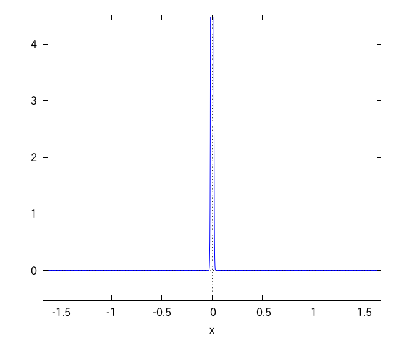
\includegraphics[keepaspectratio, width=6.5cm,height=6cm,clip]{Dirac_Delta_function3.pdf}
                        \caption{ディラックの $\delta$ 関数(1次元)の形}
                        \label{fig:delta_f2}
                    \end{center}
                \end{figure}

                        作り方は簡単.まず,面積1のグラフを用意する(図\ref{fig:delta_f24}).
                \begin{figure}[hbt]
                    \begin{center}
                        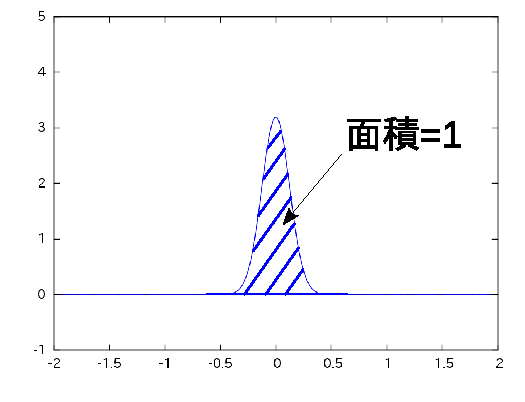
\includegraphics[keepaspectratio, width=6.5cm,height=6cm,clip]{Dirac_Delta_function5.pdf}
                        \caption{ディラックの $\delta$ 関数の作り方1}
                        \label{fig:delta_f24}
                    \end{center}
                \end{figure}

                        そして,面積1を保ちながら無限に細くしていく(図\ref{fig:delta_f33}).
                \begin{figure}[hbt]
                    \begin{center}
                        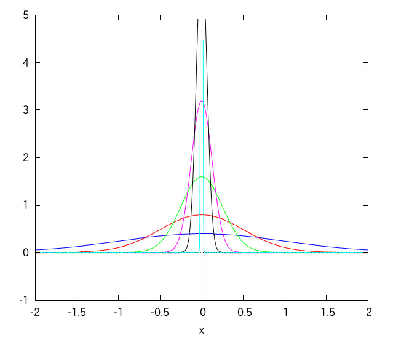
\includegraphics[keepaspectratio, width=6.5cm,height=6cm,clip]{Dirac_Delta_function4.pdf}
                        \caption{ディラックの $\delta$ 関数の作り方2}
                        \label{fig:delta_f33}
                    \end{center}
                \end{figure}
                        これで,面積が1で関数値が無限になる関数を作ることができた.

            $\delta$ 関数には次元があり,[$x^{-1}$] である.次元を持っていることを忘れやすいので,要注意.

                        ついでに,2次元の $\delta$ 関数のグラフも書いておこう.は図\ref{fig:delta_f66}下の通り.
                \begin{figure}[hbt]
                    \begin{center}
                        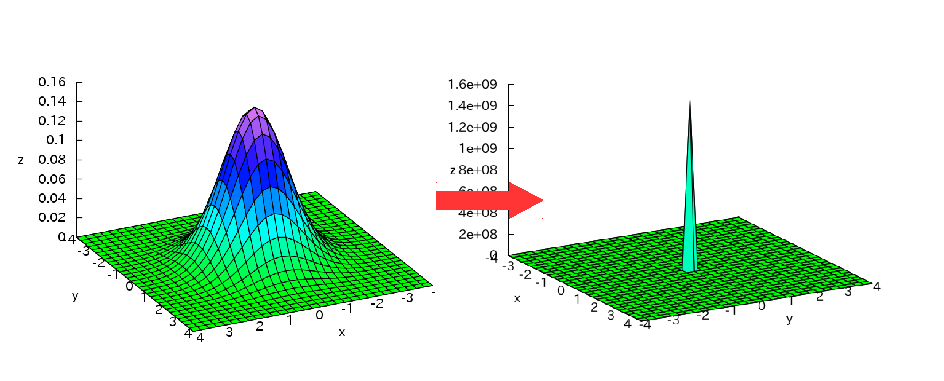
\includegraphics[keepaspectratio, width=6.5cm,height=6cm,clip]{Dirac_Delta_function6.pdf}
                        \caption{ディラックの $\delta$ 関数(2次元)の形}
                        \label{fig:delta_f66}
                    \end{center}
                \end{figure}

                        残念ながら,現実世界である3次元の $\delta$ 関数は図には描けない...

%======================================================================
%  Section
%======================================================================
\section{電流}
%======================================================================
%  SubSection
%======================================================================
    \subsection{電流のイメージ}
    おそらく,電流は説明するまでもないだろう.電気の流れのことである.い
    ままでの言葉を使えば,\textbf{電流} とは電荷の運動のことである,とい
    えよう.観測者Aに対して,荷電粒子が速度を持って運動しているとき,観測
    者Aは荷電粒子を見て,「電流が生じている」と認識するのである.この運動
    する荷電粒子は,一般に,数え切れないほど多くの数であることを想定する
    場合が多い.特に断りのない限り,電流とは,多数の荷電粒子の運動である.

    電気回路に流れる電流も多数の荷電粒子の流れであるが,この荷電粒子は導
    線中を移動することしかできない.そこでここでは,もう少し電流のイメー
    ジを拡張して,任意の空間に流れる電流を認めよう.荷電粒子は導線内部に
    しか存在できないわけではない.真空中に存在することもある.電流は導線
    だけに流れるものではない.

    電流を記号で表すときには,$I$ を用いることが多い.

    電気回路での電流のイメージは図\ref{fig:EM_Denryu01}(A)のようになろう.
    導線の中の電子をイメージしたら,図\ref{fig:EM_Denryu01}(B)の様になるかもしれない.
    しかし,実は図\ref{fig:EM_Denryu01}(B)のイメージは物性物理学的に間違っている.
    実際の電流の発生機構を説明するには原子の構造の解明や量子力学の知識が必要であり,
    それをここで考えることはできない.
    しかし,電磁気学では電荷の流れ方がどのようになっているかは説明できない.
    それとは関係なしに理論が成立している.

    電磁気学での電流とは電荷の移動であり,その場所は問われていない(導線内部である必要はない).
        具体的イメージも大事だが,ここではそれにとらわれず,抽象的な電流を考えるべきである.
        何度も言うが,電流とは空間中を移動する電荷のことである.どのように移動するかは別問題である.
        そうした抽象的な電流を考えるならば,図\ref{fig:EM_Denryu01}(B)のイメージは,
        荷電粒子の通り道を任意の空間と捉えることで,正しいイメージとなる.
        \begin{figure}[hbt]
            \begin{tabular}{cc}
                \begin{minipage}{0.5\hsize}
                    \begin{center}
                        \includegraphicsdouble{EM_Denryu01.pdf}

                        (A) 電気回路
                    \end{center}
                \end{minipage}
                \begin{minipage}{0.5\hsize}
                    \begin{center}
                        \includegraphicsdouble{EM_Denryu02.pdf}

                        (B) 一般化
                    \end{center}
                \end{minipage}
            \end{tabular}
            \caption{電流(イメージ)}
            \label{fig:EM_Denryu01}
        \end{figure}



%======================================================================
%  SubSection
%======================================================================
    \subsection{電流の定義(仮)}
        電流を数式を用いて定義しておこう.電流とは多数の点電荷の集まりの平均的な移動
        のことである.この移動を畏まった言い方をすると,次のように言える.

        ここに電流の通り道(導線)があるとしよう.
        このとき,電流を次のように定義する.
        \\
        \begin{itembox}[l]{\textbf{電流の定義(仮)}}
            \begin{itemize}
                \item 電流とは,導線の断面を単位時間1[s]に通過する
                      電荷の量を,\textbf{電流} という
                \item 電流の単位は[A]という記号で表される
                \item 電荷の単位はクーロン([C])であるので,電流の単位[A]は
                      [A]$=$[C/s]という関係がある
                \item 電流を表す標準的な記号として,このノートでは,$I$,
                      もしくは,$i$ を用いることにする
                        \footnote{
                            記号 $i$ は数学では虚数単位として用いられる
                            記号であるが,物理学や工学では電流を表すことに
                            用いることが多い(その方が一般的).なので,
                            物理学では虚数単位として,$j$ が採用されている.
                            $i$ の次のアルファベットだからだろうか.おそらく,
                            特別の意味などはないはず.文字の意味に注意しよう.
                        }
            \end{itemize}
        \end{itembox}
        \\
        \begin{figure}[hbt]
            \begin{center}
                \includegraphicslarge{EM_Denryu.pdf}
                \caption{電流(イメージ)}
                \label{fig:EM_Denryu}
            \end{center}
        \end{figure}

    \begin{memo}{注意}
        実は,この電流の単位は現在では採用されていない.
        正式な単位の定義は,後に必要な知識を説明した上で行う.
        電流に単位がないと,電流に関する事柄を扱いにくいので,
        ここではとりあえず,最も直感的で自然な定義を説明した.
        この節で「(仮)」と表現しているのは,このことによる.
    \end{memo}

%======================================================================
%  SubSection
%======================================================================
    \subsection{電流密度}
    電流とは,導線の垂直断面を,一秒間に流れる電気量として定義した.
    さらにここで,単位断面積1[m${}^{2}$]を単位時間1[s]の間に,
    どのくらいの電流が生じるかを示す \textbf{電流密度} を定義する
        \footnote{
            注意しておこう.電流密度の“密度”とは,単位面積当たりの
            密度のことである.電荷密度では,単位体積当たりの密度のこ
            とであり,両者(電荷密度と電流密度)の“密度”という語彙
            の違いは区別しておく必要がある.(次元解析をしていて,これ
            らの単位を混同してしまって,頭が混乱してしまったことがあ
            る.時間の無駄であった.)
        }.

        導線に生じている電流 $I$ が,いかなる場合でも,一様で
            \footnote{
                一様に:“むらなく”とか,“偏りなく”といった意味で使用される語彙.
            }
        あるならば,電流密度を導入することは無駄である.しかし,
        現実には,導線に生じる電流は一様ではなく,ある部分に集中的に多く
        流れていたり,ある部分には電荷の流れが全くないこともある.たしかに
        導線全体を見渡した正味の電流は一定値をとっているが,その導線の内部
        を詳細に見ることができるならば,電流にむらがあることを知るだろう.

        電流密度を $\bi(\br)$ と表す.単位は[A/m${}^{2}$]である
            \footnote{
                電荷密度 $\rho$ の単位 [C/m${}^{3}$]との違いに注意.
                電流密度は単位面積当たりの量で,電荷密度は単位体積当たり
                の量である.
            }.
        \begin{figure}[hbt]
            \begin{center}
                \includegraphicslarge{EM_DenryuMitsudo1.pdf}
                \caption{電流密度(イメージ)}
                \label{fig:EM_DenryuMitsudo1}
            \end{center}
        \end{figure}

%======================================================================
%  SubSection
%======================================================================
    \subsection{電流密度と電流の関係}
        電流 $\bI$ と電流密度 $\bi$ の関係を示そう.
        まず,電流の大きさ $I=|\bI|$ と電流密度 $\bi(\br)$ の関係を考える.

        導線の断面を $S_{l}$ とし,また,
        その一部の微小断面を $\df S_{l}$ とする
            \footnote{
                添字の $l$ は曲面 $S_{l}$ の縁となる閉曲線を表す.
                一般に,曲面は縁があるはずで,その縁は閉曲線である.
            }.
        この微小断面 $\df S_{l}$ の単位法線ベクトルを $\bn(\br)$ とかこう.

        このとき,電流密度 $\bi(\br)$ の微小断面 $\df S_{l}$ の垂直成分は
            \begin{align*}
                \bi(\br) \cdot \bn(\br) \df S_{l}
            \end{align*}
        で表現できる.そして,これを全断面 $S$ で面積分した値は,
        電流の大きさ $I$ に等しい.すなわち,
            \begin{align*}
                I = \sint_{S_{l}}\bi(\br) \cdot \bn(\br) \df S_{l}.
            \end{align*}

        まとめておこう.
        \begin{myshadebox}{電流密度と電流の関係}
            閉曲線 $l$ を縁とする曲面 $S_{l}$ を貫く電流 $I$ と,
            電流密度 $\bi(\br)$ の関係は,次式で表される.
            \begin{align}
                I = \sint_{S_{l}}\bi(\br) \cdot \bn(\br) \df S_{l}.
            \end{align}
            ここに,$\bn(\br)$ は $S_{l}$における各微小部分 $\df S_{l}$ の
            単位法線ベクトルである.
        \end{myshadebox}

        \begin{figure}[hbt]
            \begin{center}
                \includegraphicslarge{LI_si_00.pdf}
                \caption{電流と電流密度}
                \label{fig:LI_si_00}
            \end{center}
        \end{figure}

    \begin{memo}{微小面積と単位法線ベクトル}
        微小面積とは,全面積 $S$ の微小な一部分のことである.
        また,単位法線ベクトルとは,面に垂直方向で長さが1のベクトルのことである.
        \begin{figure}[hbt]
            \begin{center}
                \includegraphicslarge{EM_smollS.pdf}
                \caption{微小体積}
                \label{fig:EM_smollS}
            \end{center}
        \end{figure}
    \end{memo}

    \begin{memo}{面積分の表示方法}
        面積分は,2方向にわたる積分である.
        つまり,2つの積分変数 $u$,$v$ を
        考えたとき,これを変数に持つ関数 $f(u,\,v)$ をとし,
            \begin{align*}
                \int \left( \int f(u,\,v) \df u \right) \df v
            \end{align*}
        を計算することが,面積分を行うということである.

        つまり,$f(u,\,v)$ を最初に $u$ について積分して,その結果をさらに,
        $v$ について積分するということである.計算方法を示すには,このような
        表示の仕方が有効であるが,この表現からでは面積分であることをイメージする
        には,少々難しい.そこで,式を次ように書き換えてみる.
            \begin{align*}
                 \sint f(u,\,v) \df u \df v
            \end{align*}
        括弧をなくしただけである.そして,
        $\df S := \df u\df v$ という量を導入し,
        さらに,2回の積分を改て $\sint_{S}$ と表現することで,
            \begin{align*}
                \sint_{S} f(u,\,v) \df S
            \end{align*}
        となる.これならば,面 $S$ で面積分するというイメージが
        しやすい式の表現になった.

        ちなみに,$\df S := \df u\df v$ は \textbf{面積素} とよばれる.
    \end{memo}



%   %-----------------------------------------------------------------------------------------------
%   %  Input
%   %    File Name : PhysNote_EM_1st_RShipIandRho.tex
%   %    説明      : 電流と電荷の関係を説明する.
%   %-----------------------------------------------------------------------------------------------
        %===================================================================================================
%  Chapter : 電磁気学の基本概念
%  説明    : 電荷の存在や,電流の存在などを確認する
%===================================================================================================
%======================================================================
%  Section
%======================================================================
\section{電流と電荷の関係}
\begin{mycomment}
    \textbf{電荷} とは,電磁気現象の発生原因であり,この存在は有無をいわさず
    受け入れさせられるものである.\textbf{電流} とは,一つ,あるいは複数(多数)の
    電荷が,平均的に一方向に移動しているような現象をいう.従って,
    電流とは,電荷と観測者の相対的な速度に依存していると考えられる.つまり,
    観測者が電荷を見ているとき,その観測者の速度により,電流が生じているのか,
    単に電荷が運動せずにその場に存在しているのかが,変わってきてしまう.
    そこで,以降では,観測者の速度を0として,扱うことにする.
\end{mycomment}
%======================================================================
%  SubSection
%======================================================================
    \subsection{大局的な電荷保存則}
        \begin{mysmallsec}{電荷は突然現れることはない}
        ある領域に電荷が多数存在していることを想定しよう(図\ref{fig:Denryu_Denka_intoro}(A)参照).
        この多数の電荷の電気量の総和を,$Q(t)$ と書くことにする
            \footnote{
                電荷が多数存在するが,その個数は有限であることを想定する.
                このとき,電荷に番号付けをして,$q_{0}$,$q_{1}$,$q_{2}$,$\cdots$ の
                ように書けば,その総和 $Q(t)$ は $Q(t):=\sum_{i}^{N(t)}q_{i}$ で表せる.
                左辺の総電気量 $Q(t)$ の独立変数 $t$ は,右辺の電荷の個数が時間変化する場合($N(t)$)を
                表したものである.
            }.
        この状態から,ある程度時間が経過して,領域内部の電気量の総和が変化したとしよう.
        つまり,$Q$ の時間微分が0ではない値をとるということになる
            \footnote{
                時間変化がないということは,時間微分して0であるということである.
                例えば,速さ $v(t)$ は $v(t):=\df x(t)/\df t$($x$ は位置,$t$ は時間を表す)で
                定義されるが,位置に時間変化がない場合 $x(t)$ は一点に止まっているので,
                $x(t)=X_{\mathrm{const}}$ となり,時間によらない定数 $X_{\mathrm{const}}$ で表せる.
                この時の速度を考えると,$v(t):=\df x(t)/\df t=\df X_{\mathrm{const}}/\df t = 0$ と
                なり,位置の時間微分は0である.つまり,位置が時間変化しない(動かない)物体の
                一の時間微分は0になる.これは逆に,位置の時間微分が0であれば,
                その物体は動いていない,と言うこともできる.さらに,物体の位置の時間微分が0でない値
                を取るならば,その物体は動いていると言える.

                今回の場合,時間変化するのは領域内の総電気量 $Q(t)$ である.
            }.
        総電気量が変化したということは,その領域内部の電荷の量が変化したということである.
        つまり,個々の電荷が領域外部に出て行ったり,あるいは逆に,領域外部から電荷が入ってきた
        ということである.すなわち,
            \begin{equation*}
                \frac{\df Q(t)}{\df t} \neq 0.
            \end{equation*}
        ここで,出たり入ったりする電荷の,正味の電気量を $I(t)$ と書けば,
            \footnote{
                ここで記号として $I(t)$ を書いたのは,電流 $I(t)$をあとで定義する
                ためである.独立変数として,時間 $t$ を明示したのは,時刻によって
                生じる電流が,異なる場合を想定したからである.
            },
            \begin{equation*}
                \frac{\df Q(t)}{\df t} + I(t) = 0.
            \end{equation*}
        となるような $I(t)$ が存在することになる.要は,領域内部の総電気量 $Q(t)$ の
        時間変化に,正味の電荷の出入り $I(t)$ を足し合わせれば0であるということである.
        もっと簡単に言うと,領域内部の総電気量の変化は,外部との電荷のやり取りで
        生じるのであり,その領域内部でいきなり電荷が現れたり消えたりしない,という
        ことである(図\ref{fig:Denryu_Denka_intoro}(B)参照).この電荷の出入りを表す $I(t)$ が
        電流である.端的に言えば,ある領域内の総電気量が変化したことと,その領域に電流が生じ
        ていることとは,等価である.
        \end{mysmallsec}

        \begin{mysmallsec}{電荷保存の法則}
        実は,この考え方こそが,\textbf{電荷保存の法則} であり
            \footnote{
                略して,\textbf{電荷保存則} といわれることのほうが,一般的である.
            },今の場合は,
        \textbf{大域的(マクロ)な}視点から見た電荷保存則(脚注参照)である.後ほど,一般化して,
        \textbf{局所的な}電荷保存則も紹介することになる.

        改めて,大局的な電荷保存則を記述しておこう.
            \begin{myshadebox}{(大局的な)電荷保存則}
                ある領域内部の総電気量を $Q(t)$ とし,その内部から外部へ向かって電流 $I(t)$ が
                生じている場合,
                \begin{align}
                    \frac{\df Q(t)}{\df t} = - I(t).
                \end{align}
                という関係式が成立する.これを,
                大局的な \textbf{電荷保存の法則}(あるいは略して,\textbf{電荷保存則})という.
            \end{myshadebox}

        ここで,電流 $I(t)$ を右辺に移項した.この表現の方が,総電気量の時間変化と
        電流が等価であることを,イメージしやすいからである.また,多くの教科書で,
        この書き方がなされている.電流の符号は,領域内の総電気量が減る場合には正
        (電荷が領域内部から飛び出して,それが電流となる),
        領域内の総電気量が増える場合には負(領域内に電流が入ってきて,内部の電荷個数が増える)とする
            \footnote{
                簡単に言うと,領域から電流が外向きに生じているときに正,
                領域に電流が吸収される場合に負とする.
            }.
        \end{mysmallsec}
                \begin{figure}[hbt]
                    \begin{tabular}{cc}
                        \begin{minipage}{0.5\hsize}
                            \begin{center}
                                \includegraphicsdouble{Denryu_Denka_intoro001.pdf}

                                (A) 領域内の電荷
                            \end{center}
                        \end{minipage}
                        \begin{minipage}{0.5\hsize}
                            \begin{center}
                                \includegraphicsdouble{Denryu_Denka_intoro002.pdf}

                                (B) 電荷の出入り
                            \end{center}
                        \end{minipage}
                    \end{tabular}
                        \caption{電流と電荷}
                        \label{fig:Denryu_Denka_intoro}
                \end{figure}

%======================================================================
%  SubSection
%======================================================================
    \subsection{局所的な電荷保存則}
        電荷保存則は,局所的にも成立する法則である.理論物理学では,
        大局的表現よりも,これから説明する局所的な電荷保存則の表現
        がよく使われる.大局的な表現がすでに得られているので,そこ
        から,局所的表現を導出しよう.

        まず,電流 $I(t)$ と総電気量 $Q(t)$ を,それぞれ電流密度 $\bi$ と
        電荷密度 $\rho$ で書きなおしておこう.
            \begin{align*}
                I(t)  &=  \sint_{S} \bi \cdot \bn \df S. \\
                Q(t)  &=  \vint_{\Omega_{S}} \rho \df V.
            \end{align*}
        電流道度 $\bi$ と電荷密度 $\rho$ は,位置と時間の関数であることに注意.
            \begin{equation*}
                \bi := \bi(\br,\,t)\,,\quad \rho := \rho(\br,\,t).
            \end{equation*}
        ちなみに,電流 $I(t)$ と総電気量 $Q(t)$ の独立変数に位置 $\br$ が
        ないのは,位置で積分してしまうためである
            \footnote{
                積分変数は積分後には残らない.大局的視点から見るので,
                細かな位置を知る必要はなく,この視点で重要なのは,考察範囲
                全体の電流量や電気量なのである.これから考える局所的な量は,
                その位置も重要になる.大局的視点と局所的視点の違いは意識して
                おくべきことだろう.
            }.
        電流道度 $\bi$ と電荷密度 $\rho$ を用いると,電荷保存則は次のように書ける.
            \begin{equation*}
                 \frac{\rd}{\rd t} \left( \vint_{\Omega_{S}} \rho \df V \right)
               = - \sint_{S} \bi \cdot \bn \df S.
            \end{equation*}

        ここで,上式の右辺にガウスの定理
            \footnote{
                任意のベクトル $\bX$ に対して,
                \begin{equation*}
                      \sint_{S} \bX \cdot \bn \df S
                    = \vint_{\Omega_{S}} \ddiv \bX \cdot \bn \df V.
                \end{equation*}

                後で簡単に復習するので,そこを参照のこと.
                それでもわからなければ,数学の解説の部分を
                読むこと.さらにそれでもわからなかったら,
                ベクトル解析教科書を別途お読みください.
            }
        を適用する.
            \begin{equation*}
                  \vint_{\Omega_{S}} \frac{\rd \rho}{\rd t} \df V
                = - \vint_{\Omega_{S}} \ddiv \bi \cdot \bn \df V.
            \end{equation*}
        この式変形で,左辺の空間微分と時間微分の可換性
            \footnote{
                空間に関する微分と,時間に関する微分は計算順序を入れ替えても,
                結果は変わらないということ.
            }
        を利用した.
        この式の両辺を見ると,積分範囲が同じ体積分になっている.この等式が一般的に成り立つのは,
        両辺の被積分関数が等しいときである
            \footnote{
                数学的に示すべきことだろうが,ここでは割愛する.
            }.
            \begin{equation*}
                  \frac{\rd \rho}{\rd t} = -\ddiv \bi.
            \end{equation*}
        慣習に従って,次のように書き換える.
            \begin{align}\label{eq:bisiteki_denkahozonsoku00}
                \ddiv \bi = -\frac{\rd \rho}{\rd t}.
            \end{align}
        この式(\ref{eq:bisiteki_denkahozonsoku00})が,
        局所的な \textbf{電荷保存則} である.

        ある局所的領域
            \footnote{
                局所的領域:可能なかぎり小さくした領域のこと.あくまでも,
                直感的な言葉であり,「可能なかぎり」に特別な意味は込めていない.
                日常言語的な捉え方をしてもらいたい.
            }
        から電流が湧き出る($\ddiv \bi$)ならば,その領域内部の電荷密度は
        減少する($-(\rd \rho/\rd t)$)ということを,式で表現できている.

        改めて,まとめておこう.
            \begin{myshadebox}{(局所的な)電荷保存則}
                ある局所的領域から電流が湧き出る($\ddiv \bi$)ならば,
                その領域内部の電荷密度は減少する($-\rd \rho/\rd t$).
                \begin{align}
                    \ddiv \bi = -\frac{\rd \rho}{\rd t}.
                \end{align}
                これは,電荷保存則を局所的に表現したものである.
            \end{myshadebox}

            \begin{memo}{ガウスの定理(復習)}
                ガウスの定理:ガウスの法則とは別のもの.ガウスの定理は数学上の
                              定理である.この定理により,以下の等式が成立する.

                                任意のベクトル $\bX$ に対して,
                                \begin{equation*}
                                      \sint_{S} \bX \cdot \bn \df S
                                    = \vint_{\Omega_{S}} \ddiv \bX \cdot \bn \df V.
                                \end{equation*}

                                言葉で説明するならば,次のようなイメージになろう.
                                「任意の閉曲面 $S$ で囲まれた領域 $\Omega_{S}$ より
                                湧き出る $\ddiv \bX$ の総和は,閉曲面 $S$ の表面から
                                抜け出る正味の流出量に等しい」.
            \end{memo}



%===================================================================================================
%  Chapter : クーロンの法則
%  説明    : 電磁気学の要である,電気力=クーロン力について説明する
%===================================================================================================
\chapter{クーロンの法則}
%   %-----------------------------------------------------------------------------------------------
%   %  Input
%   %    File Name : PhysNote_EM_1st_CoulombLow.tex
%   %    説明      : 電場を導入する
%   %                を説明する.
%   %-----------------------------------------------------------------------------------------------
        %===================================================================================================
%  Chapter : クーロンの法則
%  説明    : 電磁気学の要である,電気力=クーロン力について説明する
%===================================================================================================
%======================================================================
%  Section
%======================================================================
    \section{クーロン力}\label{sec:CoulomnbForce}
%   %==================================================================
%   %  Subsection
%   %==================================================================
    \subsection{法則}
        電荷を帯びた物体が受ける,電気的な力というものが,世の中に
        存在する.これは万人が知っている事実だから,ここで改めて明
        記することは,バカバカしく感じられる.しかし,この電気的な
        力の存在は,大変重要なものである.この電気的な力のことを,
        \textbf{クーロン力} とよぶ.電気量の単位であるクーロンと同
        じ名前を持っているが,お察しのとおり,同一人物に由来するも
        のである.

        クーロン(Coulomb)は,電気的な力の性質を実験的に知ることに
        成功した
            \footnote{
                電気量の定義は,クーロン力を基にしてなされるもの
                である.
            }.
        そして,クーロンは,電気的な力が,次のような性質を持っていることを
        明らかにした.
        \\
        \begin{itembox}[l]{\textbf{クーロン力(クーロンの法則)}}
            ここに,電荷が2つあるとしよう.この2つの電荷は区別する
            ことができて,$q_{1}$,$q_{2}$ という電気量を持っている
            とする.電荷 $q_{1}$ と $q_{2}$ との距離を $r$ としたと
            き,この2つの電荷が受ける力は,以下のような規則がある.
            \begin{itemize}
                \item 2つの電荷の電気量が互いに異なる符号をもってい
                      るならば,両電荷は互いに引き合う向きに力を受
                      ける
                \item 2つの電荷の電気量が同じ符号を持っているならば,
                      両電荷は互いに反発しあう向きに力を受ける.
                \item 2つの電荷の受ける力の大きさは等しく,
                      向きは互いに逆向きである
                \item 2つの電荷が受ける力の大きさは,
                      2つの電荷の電気量の積($q_{1}q_{2}$)に比例する.
                \item 2つの電荷が受ける力の大きさは,
                      2つの電荷間の距離の2乗($r^{2}$)に反比例する.
            \end{itemize}
        \end{itembox}
        \\
        \begin{figure}[hbt]
            \begin{tabular}{cc}
                \begin{minipage}{0.5\hsize}
                    \begin{center}
                        \includegraphicsdouble{coulombs_low1.pdf}

                        (A)
                    \end{center}
                \end{minipage}
                \begin{minipage}{0.5\hsize}
                    \begin{center}
                        \includegraphicsdouble{coulombs_low2.pdf}

                        (B)
                    \end{center}
                \end{minipage}
            \end{tabular}
                        \caption{クーロン力}
                        \label{fig:coulombs_low}
        \end{figure}

        上に書いたような,クーロン力が示す性質のことを,\textbf{クーロンの法則} と
        いう.これは電磁気学の最も基本的な法則であり,大変重要な法則である.
        あとに説明する \textbf{電場} という重要な概念の導入も,
        このクーロンの法則を基にしている.

        言葉で書いてしまうと,ちょっとややこしいかもしれない.
        しかし,いきなり数式を出してしまうと,それはそれで
        尻込みしてしまうので,とりあえず言葉で説明してみた.

%   %==================================================================
%   %  Subsection
%   %==================================================================
    \subsection{定量化}
        では,次の段階に進み,クーロンの法則を数式で表現してみよう.
        数式で表現すると,とても簡潔になることを感じ取ることができる
        だろう.

        図\ref{fig:Coulombs_Force}のような状態であるとしよう.
        \begin{figure}[hbt]
            \begin{center}
                \includegraphicslarge{Coulombs_Force.pdf}
                \caption{クーロンの法則}
                \label{fig:Coulombs_Force}
            \end{center}
        \end{figure}

        2つの区別可能な電荷が存在し,それぞれの電気量が,$q_{1}$,$q_{2}$ で
        あるとする.また今後,これらの電荷自体を表現する場合にも,
        「電荷 $q_{1}$」などのように記述する
            \footnote{
                同じ記号に二つの意味を込めるのはよくないが,
                そうかと言って,無嫌味に記号を増やして読みづらくしたくも
                ない.ここでは,誤解を生むことがないと判断し,同じ記号で
                “電荷それ自体”と“その電気量”の2つを同じ記号で表すこと
                とする.
            }.
        この2つの電荷がある位置を,それぞれ $\br_{1}$,$\br_{2}$ と
        する.このとき,電荷間の距離 $r$ は,
            \begin{equation*}
                r = | \br_{2} - \br_{1} |.
            \end{equation*}
        また,電荷 $q_{2}$ から見た,電荷 $q_{1}$ の位置 $\br_{12}$は,
            \begin{equation*}
                \br_{12} = \br_{1} - \br_{2}.
            \end{equation*}
        同様に,電荷 $q_{1}$ から見た,電荷 $q_{2}$ の位置 $\br_{21}$は,
            \begin{equation*}
                \br_{21} = \br_{2} - \br_{1}.
            \end{equation*}

        「2つの電荷が受ける力は,大きさが同じで,向きが逆である.」これを
        数式で表すには,まず,大きさと向きを文字で表現すべきだ.
        同時に考えるのは難しいので,まずはクーロン力の大きさだけを考える.
        電荷 $q_{1}$ が受けるクーロン力 $F_{12}$ は,
        2点電荷の電気量の積 $q_{1}q_{2}$ に比例するので,数式的には,
            \begin{equation*}
                F_{12} = \alpha q_{1}q_{2}
            \end{equation*}
        とかける.ここに,$\alpha$ 比例定数である
            \footnote{
                この比例定数 $\alpha$ には全く意味が無い.単に
                比例を表すのに,便宜的に使ったに過ぎない.
                同じことがすぐ後に使う,$\beta$ についても言える.
                しかし,最後に現れる比例定数 $k$ については,
                重要であるので注意すべきだ.
            }.
         また同時に,
        「2つの電荷が受ける力の大きさは,2つの電荷間の距離の
        2乗($r^{2}$)に反比例する」から,
            \begin{equation*}
                F_{12} = \beta \frac{1}{r^{2}}
            \end{equation*}
        ともかける.$\beta$ も比例定数である.
        この2つの $F_{12}$ の式は矛盾なく両立する.
        この2つの式をまとめて,
            \begin{equation*}
                F_{12} = \alpha \beta \frac{q_{1}q_{2}}{r^{2}}
            \end{equation*}
        となる.ここで,式の見易さのため,比例定数 $\alpha \beta$ を
        改めて $k$ とおいて($k=\alpha \beta$),
            \begin{align}\label{eq:coulomb_force_f1_ookisa}
                F_{12} = k \frac{q_{1}q_{2}}{r^{2}}
            \end{align}
        とすれば,この式(\ref{eq:coulomb_force_f1_ookisa})によって,
        電荷 $q_{1}$ が受けるクーロン力の大きさを
        記述できたことになる.

        残りはその方向であるが,これは簡単だ.単位ベクトルを考えれば
        よい.一般のベクトル $\bA$ に対する単位ベクトルとは,大きさが $1$ で,
        その方向が $\bA$ と同じ向きのようなものである.このような単位ベクトルが
        存在したとして,$\bn$ と表そう.この時,$\bA$ は,$\bA=|\bA|\bn$ と書き
        表せる.つまり,単位ベクトル $\bn$ について解けば,
            \begin{equation*}
                \bn = \frac{\bA}{|\bA|}
            \end{equation*}
        である.

        今の場合に当てはめて考えれば,$\bA=\br_{12}$ であるから,
        単位ベクトルは
            \begin{equation*}
                \bn = \frac{\br_{12}}{|\br_{12}|}
                    = \frac{\br_{1} - \br_{2}}{|\br_{1} - \br_{2}|}
            \end{equation*}
        である.これが,電荷 $q_{1}$ が受けるクーロン力の向きを
        表している.

        これで,電荷 $q_{1}$ の受けるクーロン力の大きさと向きの
        数式的表現を,別々ではあるが,表現できた.あとは
        この2つを一緒に表せれば,完了となる.

        ここで改めて,電荷 $q_{1}$ の受ける
        クーロン力を向きも考慮して $\bF_{12}$ と表すこととすると,
        $\bF_{12}$ は,その大きさ $F_{12}$ と単位ベクトル $\bn$ を
        用いて,
            \begin{equation*}
                \bF_{12} = F_{1}\bn
            \end{equation*}
        とかける.
        これに,上で得た結果を代入すればよい.すると,
            \begin{align}\label{eq:coulomb_force_f1}
                \bF_{12} = k \frac{q_{1}q_{2}}{r^{2}} \frac{\br_{1} - \br_{2}}{|\br_{1} - \br_{2}|}
            \end{align}
        となる.この式(\ref{eq:coulomb_force_f1})が目標としていた,
        電荷 $q_{1}$ が受けるクーロン力 $\bF_{12}$を,
        式で表したものである.

        これ同様に,電荷 $q_{2}$ が受けるクーロン力 $\bF_{2}$を考えること
        ができるが,「2つの電荷の受ける力の大きさは等しく,向きは互いに逆
        向きである」ということを考慮すれば,直ちに,次式を得る.
            \begin{align*}
                \bF_{21} &= - \bF_{12} \\
                        &= - k \frac{q_{1}q_{2}}{r^{2}} \frac{\br_{1} - \br_{2}}{|\br_{1} - \br_{2}|}.
            \end{align*}
        ここで,
            \begin{align*}
                -(\br_{1} - \br_{2}) &= \br_{2} - \br_{1} \\
                |\br_{1} - \br_{2}|  &= |\br_{2} - \br_{1}| \\
                q_{1}q_{2}           &= q_{2}q_{1}
            \end{align*}
        であることに気付けば
            \footnote{
                数式を見れば当たり前のように感じるかもしれないが,重要な式である.というのも,
                この関係式は作用反作用の法則を表す数式にほかならないからである.
            },
            \begin{align}\label{eq:coulomb_force_f2}
                \bF_{21} = k \frac{q_{2}q_{1}}{r^{2}} \frac{\br_{2} - \br_{1}}{|\br_{2} - \br_{1}|}
            \end{align}
        となる.$\bF_{12}$ の式(\ref{eq:coulomb_force_f1}) と比較すると,
        添字の1と2が逆になっているだけであることに気づくだろう.

        最後に,比例定数 $k$ について記述しよう.
        この比例定数は,基準とする単位系によって値は
        変化するが,今日一般的に使用されているSI単位系を
        採用するならば,
            \begin{align}
                k = \frac{1}{4\pi\varepsilon_{0}} = 8.989 \times 10^{9}
            \end{align}
        である.$\varepsilon_{0}$ は真空の \textbf{誘電率} と言われる
        物理定数であるが,これについての解説は後回しにする.
        また,$\pi$ は円周率である.

%   %==================================================================
%   %  Subsection
%   %==================================================================
    \subsection{まとめ}
        以上の計算より得た結果をまとめよう.
        \begin{myshadebox}{クーロン力}
            ある空間に2つの電荷 $q_{1}$,$q_{2}$ が,それぞれ
            位置 $\br_{1}$,$\br_{2}$ に
            存在するとき,この2つの電荷には,次式で
            表されるような力が作用する.この力のこと
            を \textbf{クーロン力} という.

            電荷 $q_{1}$ に対して働く力は以下.
               \begin{align}
                   \bF_{12} =
                       \frac{1}{4\pi\varepsilon_{0}} \frac{q_{1}q_{2}}{r^{2}}
                           \frac{\br_{1} - \br_{2}}{|\br_{1} - \br_{2}|}.
               \end{align}

        ここに,$\varepsilon_{0}$ は真空の誘電率
           \footnote{
               詳細は後述.
           }
        である.
        \end{myshadebox}


        電荷 $q_{2}$ に対しては,以下の力が働く.
           \begin{align}
               \bF_{12} = -\bF_{21} =
                   \frac{1}{4\pi\varepsilon_{0}} \frac{q_{2}q_{1}}{r^{2}}
                       \frac{\br_{2} - \br_{1}}{|\br_{2} - \br_{1}|}.
           \end{align}


    \begin{memo}{(例)2つの点電荷同士のクーロン力}
    クーロンの法則を,より感覚的に分かるように,ここで,
    最も簡単な,2つの点電荷間に働く,クーロン力を考てみよう.

    存在する電荷が点電荷の場合,クーロンの法則は次式で表せる.
            \begin{align}
                \bF_{12}=\frac{1}{4\pi\varepsilon_{0}}
                \frac{q_{1}q_{2}}{|\br_{1}-\br_{2}|^{2}}
                \frac{\br_{1}-\br_{2}}
                     {|\br_{1}-\br_{2}|}.
            \end{align}
    より考えやすくするために,2次元で考えてみよう.座標系は,直交座標系とする.
    この場合,
        \begin{equation*}
            |\br_{1}-\br_{2}| = \sqrt{ {\left(x_{2} - x_{1}\right)}^{2}
            + {\left(y_{2} - y_{1}\right)}^{2} }
        \end{equation*}
    である.
        \begin{figure}[hbt]
            \begin{center}
                \includegraphicslarge{2point_distance.pdf}
                \caption{一般の2つの点の間の距離}
                \label{fig:2point_distance}
            \end{center}
        \end{figure}


    点電荷の配置を,$x$ 軸上にし,各電荷が $x=-1/2$,$x=1/2$ に存在しているとする.
    そうすると,2つの点電荷のそれぞれの位置ベクトルは,
    $\br_{1}  =  ( \,-1/2\,,\,0\, )$,$\br_{2}  =  ( \,1/2\,,\,0\, )$ となる.
    そうすると,
            \begin{align*}
                |\br_{1}-\br_{2}|
                &= \sqrt{ {\left(x_{2} - x_{1}\right)}^{2} + {\left(y_{2} - y_{1}\right)}^{2} } \\
                &= \sqrt{ {\left(\frac{1}{2} - \left(-\frac{1}{2}\right)\right)}^{2} + {\left(0-0\right)}^{2} } \\
                &= 1.
            \end{align*}
    電荷量の
    大きさは,両電荷ともに等しく,$1$[C] として考える.
        \begin{figure}[hbt]
            \begin{center}
                \includegraphicslarge{example_Coulombs_low1.pdf}
                \caption{例:2つの点電荷間のクーロン力}
                \label{fig:example_Coulombs_low1}
            \end{center}
        \end{figure}

    すると,クーロンの法則は,次のようになる.電荷 $q_{1}$ が,電荷 $q_{2}$ から
    受けるクーロン力 $\bF_{12}$ は
            \begin{align*}
                \bF_{12}
                &= \frac{1}{4\pi\varepsilon_{0}}
                \frac{q_{1}q_{2}}{|\br_{1}-\br_{2}|^{2}}
                \frac{\br_{1}-\br_{2}}
                     {|\br_{1}-\br_{2}|} \\
                &= \frac{1}{4\pi\varepsilon_{0}}
                \frac{1}{ 1 }
                \frac{\left( \,-1\,,\,0\, \right)}
                     { 1 } \\
                &= \frac{1}{4\pi\varepsilon_{0}} \left( \,-1\,,\,0\, \right)
            \end{align*}
    と書ける.

    クーロン力の向きは,$\left( \,-1\,,0\,\right)$ であることが
    分かった.

    以下では,クーロン力の大きさのみ($| \bF_{12} | := F_{12}$)を考えていこう.
        \begin{align*}
            |\bF_{12}|  &= F_{12} \\
                        &= \frac{1}{4\pi\varepsilon_{0}} \sqrt{(-1)^{2}+0^{2}} \\
                        &= \frac{1}{4\pi\varepsilon_{0}} \cdot 1               \\
                        &= \frac{1}{4\pi\varepsilon_{0}}
        \end{align*}

    最後に,$\varepsilon_{0}$,$\pi$ に具体的な数値を代入する.
    ここではとりあえず,
        \begin{equation*}
            \varepsilon_{0} = 8.854 \times 10^{-12}
        \end{equation*}
    であることが知られているので,この数値を使うことにする.
    しかし,どのようにして,このような数値が分かるかについては,
    後ほど,電磁気学をさらに学んでから,考えなおすことにしたい.
    $\pi$ は周知のように,
        \begin{equation*}
            \pi = 3.141
        \end{equation*}
    である.

    以上から,
            \begin{align*}
                F_{12}
                &= \frac{1}{4\pi\varepsilon_{0}} \\
                &= \frac{1}{4 \times 3.1415 \times 8.854 \times 10^{-12}} \\
                &= \frac{10^{12}}{ 222.483 }  \\
                &= 0.008989 \times 10^{12}  \\
                \therefore\quad
                F_{12}
                &= 8.989 \times 10^{9}
            \end{align*}
    を得る.

    実は,今までの計算は,単位電荷1[C]をもつ2つの点電荷が,1[m]離れて位置する
    場合のクーロン力を計算していた.つまり,
        \begin{equation*}
            \frac{q_{1}q_{2}}{r^{2}} = 1
        \end{equation*}
    となるのは,あたり前のことであった.しかし,
    あえて,座標から丁寧に計算したのは,点電荷がどのような位置に存在しても,
    同じように計算できることを,示したかったからである
        \footnote{
            この例はとても簡単だが,一般性が高い理論であることを認識
            することはできるはず.
        }.

    上の計算から,
        \begin{align}
            \frac{1}{4\varepsilon_{0} \pi} \simeq 9.0 \times 10^{9}
        \end{align}
    が分かる.この数値を用いて,クーロン力を表すと,
        \begin{align}
            F = 9.0 \times 10^{9} \times \frac{q_{1}q_{2}}{r^{2}}
        \end{align}
    となる.

    高校物理では,$k=9.0 \times 10^{9}$ と置いて,
        \begin{equation*}
            F = k \frac{q_{1}q_{2}}{r^{2}}
        \end{equation*}
    と書かれることも多い.
\end{memo}

%======================================================================
%  Section
%======================================================================
    \section{力の重ねあわせの原理}
        クーロン力は,力学的な力と同様に,重ねあわせの原理が成立
        していることが,実験的に確認されている.

        具体例で示したほうが,分かりやすい.
        3つの点電荷が存在する場合を考える.
        \begin{figure}[hbt]
            \begin{center}
                \includegraphicslarge{EM_Coulomb_KasaneAwase01.pdf}
                \caption{クーロン力(3つの点電荷)}
                \label{fig:EM_Coulomb_KasaneAwase00}
            \end{center}
        \end{figure}

        電気量 $q_{1}$,$q_{2}$,$q_{3}$ をもつ3つの点電荷
        の内,任意に2つを選ぶ.ここでは $q_{1}$ と $q_{2}$ をえらぼう.
        ここでは,例として,点電荷 $q_{1}$ が,他の点電荷 $q_{2}$ と $q_{3}$ から受ける
        クーロン力 $\bF_{1}$ を計算する.
        計算方法は,最初に点電荷 $q_{2}$ から受けるクーロン力 $\bldf_{12}$ を
        計算する.この時,$q_{3}$ はとりあえず存在しないとして考える
        (図\ref{fig:EM_Coulomb_KasaneAwase02}(A)).
            \begin{equation*}
                \bldf_{12} = \frac{1}{4\pi\varepsilon_{0}}
                           \frac{q_{2}q_{1}}{{|\br_{1} - \br_{2}|}^{2}}
                           \frac{\br_{1} - \br_{2}}{|\br_{1} - \br_{2}|}.
            \end{equation*}
        その次に,点電荷 $q_{3}$ から受けるクーロン力 $\bldf_{13}$ を
        計算する.この時,$q_{2}$ はとりあえず存在しないとして考える
        (図\ref{fig:EM_Coulomb_KasaneAwase02}(B)).
            \begin{equation*}
                \bldf_{13} = \frac{1}{4\pi\varepsilon_{0}}
                           \frac{q_{3}q_{1}}{{|\br_{1} - \br_{3}|}^{2}}
                           \frac{\br_{1} - \br_{3}}{|\br_{1} - \br_{3}|}.
            \end{equation*}
        \begin{figure}[hbt]
            \begin{tabular}{cc}
                \begin{minipage}{0.5\hsize}
                    \begin{center}
                        \includegraphicsdouble{EM_Coulomb_KasaneAwase02a.pdf}

                        (A)
                    \end{center}
                \end{minipage}
                \begin{minipage}{0.5\hsize}
                    \begin{center}
                        \includegraphicsdouble{EM_Coulomb_KasaneAwase02b.pdf}

                        (B)
                    \end{center}
                \end{minipage}
            \end{tabular}
            \caption{重ねあわせの原理(クーロン力)}
            \label{fig:EM_Coulomb_KasaneAwase02}
        \end{figure}

        最後に,今得た $\bldf_{12}$ と $\bldf_{13}$ を足し合わせれば,
        $\bF_{1}$ を得る(図\ref{fig:EM_Coulomb_KasaneAwase03}).
        \begin{align}
            \bF_{1} &=  \bldf_{12} + \bldf_{13}
        \end{align}
        \begin{figure}[hbt]
            \begin{center}
                \includegraphicslarge{EM_Coulomb_KasaneAwase03.pdf}
                \caption{クーロン力の重ねあわせの結果(3つの点電荷)}
                \label{fig:EM_Coulomb_KasaneAwase03}
            \end{center}
        \end{figure}

        同様に,
        \begin{align*}
            \bF_{2} &= \bldf_{21} + \bldf_{23}. \\
            \bF_{3} &= \bldf_{31} + \bldf_{32}.
        \end{align*}


%======================================================================
%  Section
%======================================================================
    \section{クーロンの法則($N$個の点電荷)}
    まず,一般的に表現する方法についての,説明する.

    いま,3つの電荷 $q_{1}$,$q_{2}$,$q_{3}$ について考えたが,
    一般的に表現したい場合には,点電荷の個数を具体的な自然数で
    表現することはできない.そこで,任意の自然数を表す記号 $N$ を
    用意する.

    さて,$N$ 個ある点電荷のうちで着目したい1つの点電荷を指したい
    場合を考える.この場合,あらかじめ $N$ 個の点電荷に番号付けを
    しておく.その上で,例えば「番号1の点電荷に着目して$\cdots$」な
    どといえば,特定の点電荷に着目できる.しかし,全ての電荷につい
    て一度に当てはまる一般的な性質を議論するときには,具体的な番号
    を指定して一つずつ議論するのは,とても効率が悪い
        \footnote{
            $N$ 個の電荷について,すべて同じ議論を繰り返すことになる.
        }.
    そこで,任意の番号を表す記号 $i$ を導入する
        \footnote{
            電流 $i$ と同じ記号だが,意味はぜんぜん違う.
            ここで用いられる記号 $i$ は添字である.
            しかし,文脈で誤解なく判断できるので,
            特に断りなく使われる.ちなみに,数学の虚数単位 $i$ も
            同じ記号だけど,コレとも全く違う意味である.
        }.
    これはよく
        \begin{equation*}
            i = 1,\,2,\,3,\,4,\,\cdots,\,N-1,\,N
        \end{equation*}
    と書かれる.「$i$ は1から $N$ までの自然数のうちのどれか」といった
    意味で用いられる書かれ方である.

    こうすると $N$ 個存在する,番号付けされた点電荷について,一般的に
    表記できる.つまり,$q_{i}$ と書くだけで,$q_{1}$ から $q_{N}$ の
    任意の一つを表現できるのである.これは実質的に,番号付けされた
    全ての点電荷を表していると解釈できる.
        \begin{figure}[hbt]
            \begin{center}
                \includegraphicslarge{EM_GenKasaneAwase.pdf}
                \caption{$N$ 個の点電荷の番号付け}
                \label{fig:EM_GenKasaneAwase}
            \end{center}
        \end{figure}

    ようやく本題に入れる.
    $N$ 個の点電荷が存在するときは,クーロン力についても,
    力の重ね合わせの原理が成立している.
    すなわち,位置 $\br_{i}$ に存在する電気量 $q_{i}$ を持った点電荷が,
    各点電荷から受ける力 $\bldf_{ij}$ の合力 $\bF_{i}(\br_{i})$ は次式
    で表現される.

    しかし,ここで注意が必要である.気が付いているだろうか.
    $j=i$ の場合に,どうなるかを考えてみただろうか.$j=i$,
    つまり,クーロン力が $\bldi{f}_{ii}$ と表されることになり,
    これは電荷自分自信から受ける
    クーロン力を表す.クーロンの法則は,あくまでも2つの点電荷から
    なる系についての法則である.そこには,1つの電荷がそれ自身に与える
    クーロン力というものは,説明されていない.
    なので,ここでは,$j=i$ の場合を除おくことにしよう
        \footnote{
            しかし,クーロンの法則に1つの電荷が自身に与える
            クーロン力について,何も説明されていないからとい
            って,それが生じないと結論されるわけではない.
            実際,これは「自己力」として,よく取り上げられる
            問題である.古典的な電磁気学(量子力学的でない電磁気学)
            では,この自己力は $\bld{0}$ となることが説明できが,
            これについては,後ほど考えることにしたい.
        }.
        \begin{myshadebox}{クーロンの法則($N$個の点電荷)}
            点電荷が $N$ 個存在するとき,この点電荷に適当に番号付けをする.
            この時,番号 $i$ の点電荷にかかるクーロン力は,次式で表せる.
            \begin{align}
                \bF_{i}(\br_{i})&=\sum_{j=1}^{N}\bldf_{ij} \notag \\
                &=\sum_{j=1,j\neq i}^{N}\frac{1}{4\pi\varepsilon_{0}}
                \frac{q_{i}q_{j}}{|\br_{i}-\br_{j}|^{2}}
                \frac{\br_{i}-\br_{j}}
                     {|\br_{i}-\br_{j}|}
            \end{align}
            ここで,$ \displaystyle \sum_{j=1,j\neq i}$ という表現は,
            $j=i$ の場合のみを除いた,$j=1$ から $N$ までの総和を意味する
        \end{myshadebox}

        \begin{figure}[hbt]
            \begin{center}
                \includegraphicslarge{EM_CoulombN.pdf}
                \caption{クーロンの法則($N$個の点電荷)}
                \label{fig:EM_CoulombN}
            \end{center}
        \end{figure}

        \begin{memo}{和の記号: $\sum_{j=1,j\neq i}^{N}$ の注意}
            例えば,$i=3$ 番目を考えると,
                \begin{equation*}
                    \sum_{j=1,j\neq i}^{N} 2j
                    = 2 \cdot 1 +  2 \cdot 2 + 2 \cdot 4 + \cdots + 2 \cdots N
                \end{equation*}
            と展開される.3番目の項が,無いことに注目してもらいたい.

            さらに,計算開始の番号が $j=1$ であることが,明らかな場合,
            省略して,
                \begin{equation*}
                    \sum_{j\neq i}^{N} 2j
                    = 2 \cdot 1 +  2 \cdot 2 + 2 \cdot 4 + \cdots + 2 \cdots N
                \end{equation*}
            のように書かれることもある.
        \end{memo}


%======================================================================
%  Section
%======================================================================
    \section{クーロンの法則(電荷の連続分布)}
    電荷が連続分布しているならば,電荷密度 $\rho(\br^{*})$ で考えるほうがよい.
    このとき,和の記号は積分記号に変わる.また,点電荷が連続
    分布していることから,その位置 $\br_{i}$ を示すのではなく,
    任意の位置を示す必要がある.そこで,添字 $i$ を取り払って,
    $\br$ と表すことにする.以下の式は,位置 $\br$ でのクーロン力を
    表す.さらに,積分するときの変数記号を,$\br^{*}$ で表す.

    すると,電荷が連続分布する場合のクーロンの法則は,以下のように
    表現できる.
    \begin{myshadebox}{クーロン力(電荷の連続分布)}
        \begin{align}\label{coulomb'slow2}
            \bF(\br)
            &=\int_\Omega \frac{1}{4\pi\varepsilon_{0}}
            \frac{q\rho(\br^{*})}{|\br-\br^{*}|^{2}}
            \frac{\br-\br^{*}}
                 {|\br-\br^{*}|}\df V^{*}.
        \end{align}
    \end{myshadebox}

    ここで,積分はアスタリスク記号「$^{*}$」ついたものについて行う
        \footnote{
            アスタリスク(Asterisk): 記号の名前.「アステリスク」とも言われる.
            「アステリスク」という呼び方は,コンピュータ関係の技術者によく使われる
            (そのままローマ字読みすると,そうなる).本ノートでは,「アスタリスク」と
            記述していこう.
        }.
    また,式の $\Omega$ は任意の領域である.これが,電荷が連続分布し
    ている場所における,電気量 $q$ の電荷が受ける力である.
        \begin{figure}[hbt]
            \begin{tabular}{cc}
                \begin{minipage}{0.5\hsize}
                    \begin{center}
                        \includegraphicsdouble{EM_CoulombRho.pdf}

                        (A)
                    \end{center}
                \end{minipage}
                \begin{minipage}{0.5\hsize}
                    \begin{center}
                        \includegraphicsdouble{EM_DenkamdV.pdf}

                        (B) [再揚(図\ref{fig:EM_DenkamdV})]
                    \end{center}
                \end{minipage}
            \end{tabular}
            \caption{クーロンの法則(電荷の連続分布)}
            \label{fig:EM_CoulombRho}
        \end{figure}


%======================================================================
%  Section
%======================================================================
\section{クーロン力(電気的な力)と力学的な力}
    クーロンの法則:
        \begin{align*}
            \bF(\br)
            &=\int_\Omega \frac{1}{4\pi\varepsilon_{0}}
            \frac{q\rho(\br^{*})}{|\br-\br^{*}|^{2}}
            \frac{\br-\br^{*}}
                 {|\br-\br^{*}|}\df V^{*}
        \end{align*}
    の左辺の力はニュートン力学
    で導入した力学的な力のことであり
        \footnote{
            力学的な力とは,運動方程式で導入される力を指している.
        },
    電気的な力ではない.それに対して,右辺は,クーロンの法則によって示される電気的な力である.
    要するに,右辺の式で示される力と左辺で示される力は,
    定義がことなるものである.この式の等号は,右辺と左辺の
    種類の異なる力が物理学的に等価に扱えることを示すものである.
    右辺のクーロン力の原因は電荷だから,電気的な力であるが,
    電気的な力を直接的に測定することはできない
        \footnote{
            ニュートン力学で導入た力は,例えば,天秤やバネ秤を使って測定できる.
            しかし,クーロン力は直接測定する方法がない.
        }
    .だから,
    測定のできる力学的に力に換算して,電気的な力を表現するのであ
    る.

    クーロンの法則の前提条件として,「固定されてる点電荷にはたら
    く力」というものがある.この条件は,クーロン力によって点電荷
    が運動しないように設定した条件である.力を受けている物体は加
    速度運動するということが,ニュートン運動方程式の意味するとこであ
    った.クーロン力を受けている電荷は固定されていなければ加速度
    運動してしまうのである.だから,固定されているという条件をつ
    けたのである.固定されているということは,クーロン力を受けな
    がら静止しているということである.従って,クーロン力と釣り合
    う外力が働いていることになる.クーロンの法則を確認するには,電
    荷の電気量や,電荷間の距離をいろいろ変えてみて,そのときに電荷
    を固定するのに必要な外力を測定すればよい.


%===================================================================================================
%  Chapter : 電場
%  説明    : 電場の概念を導入るすことで,遠隔作用のクーロンの法則を,近接作用的に書き換える
%===================================================================================================
\chapter{電場}
%   %-----------------------------------------------------------------------------------------------
%   %  Input
%   %    File Name : PhysNote_EM_1st_Elefield.tex
%   %    説明      : 電場を導入する
%   %                を説明する.
%   %-----------------------------------------------------------------------------------------------
        %===================================================================================================
%  Chapter : 電場
%  説明    : 電場の概念を導入るすことで,遠隔作用のクーロンの法則を,近接作用的に書き換える
%===================================================================================================
%       %======================================================================
%       %  Section
%       %======================================================================
            \section{作用の伝わり方}
            \subsection{遠隔作用}
            2つの点電荷が存在する場合を考える.
            この2つの電荷は距離 $r$ を隔てて固定されているものとする.
            このように設定された2つの電荷間には,$r$ の距離を通してクーロン力が
            伝わると考えられる.このようなことを,
            「クーロン力は \textbf{遠隔作用} で伝わる」という.
            この考え方によると,クーロン力は一瞬にして伝わるとされる.点電荷間の距離が
            どんなに大きくても,クーロン力は一瞬で伝わるのである.この考え方は
            納得がいかないことだろう.実際,クーロン力が伝わるには時間が掛かる
            ことが示されている.従って,クーロンの法則は,力の遠隔作用という
            点で問題を抱えていることになる.

            \subsection{近接作用}
            遠隔作用であるクーロン力を,より直感的に馴染む \textbf{近接作用} となるように
            書き換える.近接作用は,その名の通り,電荷はその隣りの空間から影響を受ける
            という考え方で,遠くにある電荷から瞬間的にクーロン力が伝わるのではなく,
            だんだんとクーロン力が伝わってくると考えるのである.しかし,近接作用を
            採用するとなると,そのクーロン力を伝えるための「何か」が必要になってくる.
            例えば,音波は空気を通して伝わるように,クーロン力も音波に対する空気のような,
            それを伝えるための媒質があるとすべきだ.
            そのために導入するのが \textbf{電場} という概念である.クーロン力は,
            電場を通して伝達するのである.以下で,この電場という考え方を
            説明していく.


%       %======================================================================
%       %  Section
%       %======================================================================
            \section{電場(1個の点電荷)}
%   %==========================================================================
%   %  Subsection
%   %==========================================================================
    \subsection{2つの点電荷間のクーロン力}
                これから,\textbf{電場} という概念を説明したいのだけど,初めて学習
                する場合に,いきなり一般的な定義を提示していまうと,数学的な演算のみ
                に思考が傾いてしまいがちだし,もしかすると,“難しい”概念なのだ感じ
                てしまうかもしれない.そこで,このノートでも,他の多くの教科書と同様
                に,段階を踏んで電場という概念を説明していきたい.

                最初に考えるのは,2つの点電荷のみが存在する場合についてである.

                クーロンの法則は,一方の点電荷が他方の点電荷にクーロン力を与える,
                というものであった.従って,クーロン力とは2つ以上の点電荷が存在し
                て初めて観測される力である.簡単のために,2つの点電荷だけが存在す
                る場合を考える.この2つの点電荷のうちの1つの点電荷を空間に固定して,
                残りの電荷は人間がいつでも好きな場所におくことができるようにする.
                この自由に動かせる電荷を固定されている電荷の周りの様々な場所に置い
                てみると,置く場所によって受けるクーロン力が異なってくる.なぜなら,
                点電荷間の距離が異なるからである.しかし,自由に動かせる点電荷の場
                所を1つだけ指定すれば,この点電荷の受けるクーロン力は一意に決まる
                    \footnote{
                        「一意に決まる」というのは,解が必ずひとつに定まることをいう.
                    }.

                これが,「電場」という発想の源となる.自由に動かせる点電荷を利用し
                て,『固定された点電荷が,その周りの空間に作る電気的な世界を見よう』
                というのだ.自由に動かせる点電荷を様々な場所に置いてみて,その場所
                で固定された電荷から受けるクーロン力を記録していくのである.もちろ
                ん,全ての場所に自由に動かせる点電荷を置いていく.実際は無理だが,
                頭の中では簡単にできることである.一種の思考実験であると考えればよ
                い.このようにして作った記録は,点電荷特有のものになる.この記録の
                ことを点電荷の電場とよぶことにしようというのである.
                    \begin{figure}[hbt]
                        \begin{tabular}{cc}
                            \begin{minipage}{0.5\hsize}
                                \begin{center}
                                    \includegraphicsdouble{denba_intro.pdf}
                                    \caption{試験電荷の受ける力}
                                    \label{fig:siken_denka_ukerutikara}
                                \end{center}
                            \end{minipage}
                            \begin{minipage}{0.5\hsize}
                                \begin{center}
                                    \includegraphicsdouble{denba_intro2.pdf}
                                    \caption{試験電荷の受ける力の記録}
                                    \label{fig:denba_intro2}
                                \end{center}
                            \end{minipage}
                        \end{tabular}
                    \end{figure}

%   %==========================================================================
%   %  Subsection
%   %==========================================================================
    \subsection{定量化}
                定量化してみよう.固定された点電荷の電気量を $q_{0}$ とし,
                位置を $\br_{0}$ とする.また,
                自由に動かせる点電荷の電気量を $q_{x}$ とし,
                位置を $\br_{x}$ とする.
                このとき,自由に動かさせる電荷が 固定された電荷から受けるクーロン力は
                        \begin{align}
                            \bF(\br_{x})=\frac{1}{4\pi\varepsilon_{0}}
                            \frac{q_{x}q_{0}}{|\br_{0}-\br_{x}|^{2}}
                            \frac{\br_{0}-\br_{x}}
                                 {|\br_{0}-\br_{x}|}
                        \end{align}
                と書ける.ここで,$\bF(\br_{x})$ と
                書いたのは,$\br_{x}$ が自由に動かせることを強調するためである.
                ここで,この式を眺めていると,以下のように変形しても示されているよさそうであ
                ることに気付く.
                        \begin{align}
                            \bF(\br_{x})=q_{x}\left(\frac{1}{4\pi\varepsilon_{0}}
                            \frac{q_{0}}{|\br_{0}-\br_{x}|^{2}}
                            \frac{\br_{0}-\br_{x}}
                                 {|\br_{0}-\br_{x}|}\right).
                        \end{align}
                この式の 括弧の中身は $\br_{x}$ の関数である.
                だから,括弧の中身を $\bE_{0}(\br_{x})$ とおくことができる.
                        \begin{align}
                            \bE_{0}(\br_{x})=\frac{1}{4\pi\varepsilon_{0}}
                            \frac{q_{0}}{|\br_{0}-\br_{x}|^{2}}
                            \frac{\br_{0}-\br_{x}}
                                 {|\br_{0}-\br_{x}|}.
                        \end{align}
                ここで,関数の添え字に「固定」とつけた理由は,固定された点電荷が作るも
                のであることを忘れないようにするためである.
                このように定義された関数は,固定された点電荷特有の関数である.従ってこ
                の関数は,固定された電荷が
                その周りの空間に作る電気的な世界を記述していると考えられる.このような
                関数を,点電荷の \textbf{電場} と
                いうのである.電場を用いると
                        \begin{align}
                            \bF(\br_{x})
                            =q_{x}\bE_{0}(\br_{x})
                        \end{align}
                とできる.

%   %==========================================================================
%   %  Subsection
%   %==========================================================================
    \subsection{単位電荷が及ぼすクーロン力}
                $q_{x}=1$ とすると,
                        \begin{align}
                            \bF(\br_{x})
                            =\bE_{0}(\br_{x})
                        \end{align}
                となって,自由に動かせる点電荷に働く力が,電場に等しくなる.
                このことは,電荷の単位が [C] であったことを思い出せば,
                『電場は 1[C]の電荷に働くクーロン力に等しい』と言える.
                従って,今までは点電荷の作る電場を考えてきたが,たとえ電場の
                関数の具体的な形が分からなくても,1[C] の電荷を様々な場所に置いて
                その場所でのクーロン力を測ることによって,
                電場を知ることができるのである.このように使われる「1[C] の電荷」のことを,
                \textbf{試験電荷} という.何となくではあるが,
                電場のイメージができたところで,
                以下で一般的な電場の定義を与えることにする.

                $'$ が付いた記号は固定電荷についての情報を表し,
                何も付いていない記号は試験電荷についての情報を表す.
                すると,次のように表現を改め直せる
                    \footnote{
                        記号が変わっただけで,
                        書いていることは同じなのだけど.
                        こう表したほうが,
                        カッコイイし,見ためもスッキリとしていて見やすい.
                    }.
                    \begin{align*}
                        \bE(\br) := \frac{1}{4\pi\varepsilon_{0}}
                                    \frac{q'}{|\br-\br'|^{2}}
                                    \frac{\br-\br'}{|\br-\br'|}.
                    \end{align*}
                    \begin{myshadebox}{電場(1個の点電荷)}
                        1個の点電荷のつくる電場 $\bE(\br)$ は次式で表現される.
                        \begin{align*}
                            \bE(\br) := \frac{1}{4\pi\varepsilon_{0}}
                                        \frac{q'}{|\br-\br'|^{2}}
                                        \frac{\br-\br'}{|\br-\br'|}.
                        \end{align*}

                        ここで,
                            $\br$ は試験電荷を置く位置(任意の位置),
                            $q'$ は固定点電荷のもつ電気量,
                            $\br'$ は固定電荷の位置
                        である.
                    \end{myshadebox}


%       %======================================================================
%       %  Section
%       %======================================================================
            \section{電場($N$ 個の点電荷)}
            状況を少し一般化させて,$N$ 個の固定された点電荷が作る電場を考える.
            電場の定義がクーロン力を基にすることには変わらない
                \footnote{
                    そもそも,電場はクーロンの法則をより直感てきに
                    なじむように発展させた概念なのである.
                }.
            だから,クーロン力が重ね合わせの原理に従う以上,
            これに付随して電場も重ね合わせの原理に従わねばならない.
            つまり,点電荷の個数が1個から $N$ 個に増えようと,
            別に新しい考え方を導入する必要はない.単に,試験電荷が
            一つひとつの固定電荷がつくる電場を計算し,最後にそれらを全て
            加えあわせればよいだけである.
            つまり,固定された $N$ 個の点電荷が作る電場は次式で表現できる.
                \begin{align}
                    \bE(\br)&=\sum_{i=1}^{N}\frac{1}{4\pi\varepsilon_{0}}
                    \frac{q'_{i}}{|\br-\br'_{i}|^{2}}
                    \frac{\br-\br'_{i}}
                         {|\br-\br'_{i}|}
                \end{align}
            と書ける.それは,クーロン力が重ね合わせの原理を満たしてい
            ることからわかる.
                \begin{myshadebox}{電場($N$ 個の点電荷)}
                    $N$ 個の点電荷のつくる電場 $\bE(\br)$ は次式で表現される.
                    \begin{align}\label{denba_huku}
                        \bE(\br)&=\sum_{i=1}^{N}\frac{1}{4\pi\varepsilon_{0}}
                        \frac{q'_{i}}{|\br-\br'_{i}|^{2}}
                        \frac{\br-\br'_{i}}
                             {|\br-\br'_{i}|}
                    \end{align}

                    ここで,
                        $\br$ は試験電荷を置く位置(任意の位置),
                        $q'_{i}$ は固定点電荷のそれぞれのもつ電気量,
                        $\br'_{i}$ は固定電荷のそれぞれの位置
                    である.
                \end{myshadebox}

%       %======================================================================
%       %  Section
%       %======================================================================
            \section{電場(電荷の連続分布)}
            電荷が連続分布している場所において,電気量 $q$ をもつ電荷
            が受ける力は,式(\ref{coulomb'slow2})によって,
                \begin{align}
                    \bF(\br)
                    &=\int_\Omega \frac{1}{4\pi\varepsilon_{0}}
                    \frac{q\rho(\br^{*})}{|\br-\br^{*}|^{2}}
                    \frac{\br-\br^{*}}
                         {|\br-\br^{*}|}\df V^{*}
                \end{align}
            のように書かれる.この $q$ 電荷は \textbf{試験電荷} である.
            試験電荷 $q$ を用意して,この試験電荷が各点で
            受ける力を考えることによって,周り電気的様子を観測するのである.
            この式を,以下のように変形する.$q$ は積分には関係のない定数であるので,
            で積分記号の前に出せて
                \begin{align}
                    \bF(\br)
                    &=q\int_\Omega \frac{1}{4\pi\varepsilon_{0}}
                    \frac{\rho(\br^{*})}{|\br-\br^{*}|^{2}}
                    \frac{\br-\br^{*}}
                         {|\br-\br^{*}|}\df V^{*}
                \end{align}
            と書ける.ここで,以下の量を定義する.

            点電荷が連続的に分布している場合,電場 $\bE(\br)$ は電荷密度 $\rho(\br^{*})$ を
            用いて,以下の数式で定義できる.
                \begin{align}
                    \bE(\br)
                    :=\int_\Omega \frac{1}{4\pi\varepsilon_{0}}
                    \frac{\rho(\br^{*})}{|\br-\br^{*}|^{2}}
                    \frac{\br-\br^{*}}
                    {|\br-\br^{*}|}\df V^{*}.
                \end{align}
             ここに,上付きのアスタリスク ${}^{*}$ が付いている
             変数について積分を実行する
                 \footnote{
                     アスタリスクなしの $\br$ は任意の位置を
                     示す,関数の変数である.上付きのアスタリスクが
                     ついた $\br^{*}$ は電荷が分布している場所を表す
                     積分変数である
                     (積分変数はどんな記号を用いても結果にはなんの影響も
                     与えないが,位置についての積分であることを強調したいため,
                     $\br^{*}$ という書き方をした).
                 }.

            このように電場 $\bE(\br)$ を定義することで,クーロンの法則は
                \begin{equation*}
                    \bF(\br) = q \bE(\br)
                \end{equation*}
            と書ける.特に,単位電荷 $q=1$[C] の場合,
                \begin{equation*}
                    \bF(\br) = \bE(\br)
                \end{equation*}
            となり,クーロン力 $\bF(\br)$ がそのまま電場 $\bE(\br)$ を表す式になる.
                \begin{myshadebox}{電場(電荷の連続分布)}
                    点電荷が連続的に分布している場合,電場は電荷密度 $\rho(\br^{*})$ を
                    用いて,以下の数式で定義できる.
                    \begin{align}\label{denba}
                        \bE(\br)
                        :=\int_\Omega \frac{1}{4\pi\varepsilon_{0}}
                        \frac{\rho(\br^{*})}{|\br-\br^{*}|^{2}}
                        \frac{\br-\br^{*}}
                        {|\br-\br^{*}|}\df V^{*}.
                    \end{align}
                    ここに,上付きのアスタリスク ${}^{*}$ が付いている
                    変数について積分を実行する.
                \end{myshadebox}


%       %======================================================================
%       %  Section
%       %======================================================================
            \section{電場(一般化)}
            一般に,電気量 $q$ をもつ点電荷は周囲のその他の
            電荷,あるいは,電荷密度からクーロン力を受ける.
            このクーロン力 $\bF(\br,q)$ は
                \footnote{
                    ここで,独立変数として,点電荷の位置 $\br$ だけ
                    ではなく,点電荷の電気量 $q$ もすぐ後の都合で,
                    明記しておく(あとで,$q$ を0の極限に持ってい
                    く必要が出てくる).
                },
                \begin{align*}
                    \bF(\br,q)=q\bE(\br)
                \end{align*}
            と表現できる
                \footnote{
                    $\bE(\br)$ は $\br$ のみを独立変数に持つ
                    関数である.
                }.

            電場はクーロンの法則を満たすように定義されることに注意する.
            具体的には,式(\ref{denba})である.クーロンの法則で表せば,
                \begin{align}
                    \bE(\br)=\frac{\bF(\br)}{q}
                \end{align}
            である.電荷分布が決定されれば,各位置でのクーロン力は
            一意に決まる.従って,電場についても同様なことがいえる.

            さらに細かいことをいえば,電気量 $q$ の電荷は,
            自身から生じる電場により周囲の電場を歪ませてしまう.
            そこで,電気量 $q$ を 0 に近づける.すると,
            これは以下のように表現できる.
                \begin{align*}
                    \bE(\br)=\frac{\rd\bF(\br,q)}{\rd q}.
                \end{align*}

            ここでは,時間変化しないクーロン力で電場を考えている.
            クーロンの法則は,点電荷の位置が時間変化しないという条
            件の下で成り立つ法則である.従って,このクーロン力によって
            定義された電場もまた,時間変化を考慮していない.
            時間変化する電場については後述する.
                \begin{myshadebox}{電場(一般的な定義)}
                一般に,電気量 $q$ をもつ点電荷が周囲から受ける
                クーロン力 $\bF(\br,q)$ を用いて,次式で \textbf{電場} を
                定義する.
                    \begin{align}\label{denba_teigi}
                        \bE(\br, t)
                        :=\frac{\rd\bF(\br,q)}{\rd q}.
                    \end{align}
                \end{myshadebox}


                \begin{memo}{(例)点電荷の作る電場}
                    電場の定義の式(\ref{denba_teigi})を用いて,
                    点電荷 $q$ の作る電場を定義から求めてみる.
                    試験電荷の電気量を $q'$ とする.
                    すると,クーロンの法則により,クーロン力は
                            \begin{align}
                                \bF=\frac{1}{4\pi\varepsilon_{0}}
                                \frac{qq'}{|\br-\br'|^{2}}
                                \frac{\br-\br'}
                                     {|\br-\br'|}
                            \end{align}
                    と書ける.ここで,$\br'$ は試験電荷 $q'$ の位置である.このクーロン力を用いて,
                    電場は以下のように計算される.
                        \begin{align}\label{tendenka_denba}
                            \bE(\br)
                            &= \frac{\rd\bF(\br,q')}{\rd q'} \notag \\
                            &= \frac{\rd}{\rd q'}\left(\frac{1}{4\pi\varepsilon_{0}}
                                \frac{qq'}{|\br-\br'|^{2}}
                                \frac{\br-\br'}
                                     {|\br-\br'|}\right)\notag \\ \notag \\
                            &= \frac{1}{4\pi\varepsilon_{0}}
                                \frac{q}{|\br-\br'|^{2}}
                                \frac{\br-\br'}
                                     {|\br-\br'|}\notag \\ \notag \\
                            \therefore \quad
                            \bE(\br)
                            &= \frac{1}{4\pi\varepsilon_{0}}
                                \frac{q}{|\br-\br'|^{2}}
                                \frac{\br-\br'}
                                     {|\br-\br'|}
                        \end{align}
                    この式(\ref{tendenka_denba})が,点電荷の作る電場を表す式である.
                    この点電荷の存在する場所に対して,電場は点対称であることが確認できる.
                \end{memo}

%       %======================================================================
%       %  Section
%       %======================================================================
            \section{時間変化する電場}
                例えば,電荷密度が常に均一でなく,時間的に変化して電荷の存在する
                場所に局所的な偏りが生じる場合,当然として,その電荷分布より生じる
                電場も時間的に変化する.

                クーロン力の時間変化の原因は,電荷密度 $\rho$ の時間変化であり,
                この他に時間変化の原因となるものはない.従って,電荷密度の
                独立変数として,時間 $t$ を書き加えてやれば良い.つまり,
                    \begin{equation*}
                        \rho := \rho(\br, t)
                    \end{equation*}
                とする.このとき,時間変化するクーロン力は,時間を表す
                変数 $t$ をその独立変数を明示して,$\bF(\br, t)$ と
                書くことにすれば,
                    \begin{align}
                        \bF(\br, t)
                        &=q\int_\Omega \frac{1}{4\pi\varepsilon_{0}}
                        \frac{\rho(\br^{*}, t)}{|\br-\br^{*}|^{2}}
                        \frac{\br-\br^{*}}
                             {|\br-\br^{*}|}\df V^{*}
                    \end{align}
                とかける.

                すると,時間変化する電場 $\bE(\br, t)$ は,自然と以下のように定義できる.
                    \begin{align}
                        \bE(\br, t)
                        :=\int_\Omega \frac{1}{4\pi\varepsilon_{0}}
                        \frac{\rho(\br^{*}, t)}{|\br-\br^{*}|^{2}}
                        \frac{\br-\br^{*}}
                        {|\br-\br^{*}|}\df V^{*}.
                    \end{align}

                この時間変化する電場を使うと,クーロン力は
                    \begin{equation*}
                        \bF(\br,t) = q\bE(\br, t)
                    \end{equation*}
                 で表せる.単純に,独立変数に時間 $t$ を書き加えるだけで済む.

                電場が時間的に変化する場合でも,上に説明したような,電場の一般
                的な定義が成立する
                    \footnote{
                        だから「一般的な」という副詞をつけられる.
                    }.
                数式は,以下のようになる.
                    \begin{align}\label{denba_teigi_3}
                        \bE(\br)
                        :=\frac{\rd\bF(\br, q, t)}{\rd q}.
                    \end{align}
                これも単に独立変数に $t$ を明記しただけにすぎない.
                \begin{myshadebox}{電場(時間変化する場合)}
                一般に,電気量 $q$ をもつ点電荷が周囲から受ける
                クーロン力 $\bF(\br,q)$ を用いて,次式で \textbf{電場} を
                定義する.
                    \begin{align}\label{denba_teigi_4_t}
                        \bE(\br)
                        :=\frac{\rd\bF(\br,q, t)}{\rd q}.
                    \end{align}
                \end{myshadebox}


%       %======================================================================
%       %  Section
%       %======================================================================
            \section{電場の定性的なイメージ}
%       %======================================================================
%       %  Subsection
%       %======================================================================
        \subsection{イメージ}
                静電場はある特定の位置を指定すると,決まった方向に決まった強さ
                を示す.この性質は,電場を流体のようにイメージすることを可能に
                する.流体とは,水とか空気とかのことである.つまり,水や空気の
                流れのように電場のイメージをするのである.電場は目に見えないの
                で,このように考えるより方法がない.また,このイメージで注意す
                ることは,「電場には水のような媒質がない」ことである
                     \footnote{
                        アインシュタインらによる,「エーテル存在の否定」をこのノートで
                        は受け入れる.今でレこれが当たり前.
                     }.
                これは,電場と流体の大きな違いの1つである.水の流れとは,要す
                るに多くの水分子($\mathrm{H_{2}O}$)の移動だが,電場にはこの分子
                に当るものは存在しないことである.ここが電場のイメージが難しい
                ところである.でも,電荷を電場内に置いたときに,その電場から電
                荷がクーロン力を受けて運動するのだから,そこには何らかの「流れ
                的なもの」があると考えてよいだろう.その流れのようなものが,電場で
                あると解釈するのである.

                すると,「何が電場を発生させているのか」という疑問が生まれる.
                この疑問に答えるのが,後の章で考える 電場に対するガウスの法則
                である.
                \begin{figure}[hbt]
                    \begin{center}
                        \includegraphicsdouble{denba_image.pdf}
                        \caption{電場の流線(電気力線)のイメージ}
                        \label{fig:denba_image}
                    \end{center}
                \end{figure}


%       %======================================================================
%       %  Subsection
%       %======================================================================
        \subsection{電気力線(電場の可視化)}\label{subsec:dennki_rikisenn}
            電場は直接見ることのできない,抽象的な概念である.しかし非常に重要な
            概念であり,この電場という言う概念があるからこそ,電磁気現象を統一的に
            把握できる.ならば,“どうにかして電場を可視化したい”と思う
            ことだろう.実際に,ファラデーはこれを可視化することを試みていて,
            これは今日の形で言うと,\textbf{電気力線} とよばれる概念になる.
            あまりにも複雑な電場を想定しても,ただ話が複雑になるだけなので,
            1個の点電荷より生じる電場の電気力線を見てみることにしよう.
            \begin{figure}[hbt]
                \begin{tabular}{cc}
                    \begin{minipage}{0.3\hsize}
                        \begin{center}
                            \includegraphicsdouble{denriki_gazoukensaku.pdf}

                            (A) 砂鉄を使う
                        \end{center}
                    \end{minipage}
                    \begin{minipage}{0.7\hsize}
                        \begin{center}
                            \includegraphicsdouble{denriki_gazoukensaku_2.pdf}

                            (B) 電気力線
                        \end{center}
                    \end{minipage}
                \end{tabular}
                \caption{点電荷が作る電気力線(平面)\label{fig:denriki1111}}
            \end{figure}

            点電荷が作る電場の平面的イメージは図\ref{fig:denriki1111}(A),(B)のようである
                \footnote{
                    図\ref{fig:denriki1111}(A)は
                        \url{http://www.kleen-tec.co.jp/elec/elec.htm}
                    より(2008.08.23現在),
                    図\ref{fig:denriki1111}(B)は
                        \url{http://www.keirinkan.com/kori/kori_physics/kori_physics_1_kaitei/index.html}
                    より(2008.08.23現在).
                }.
            左の写真では,電場の向きを捉えることはできないが,ここに試験電荷を置いたときに,
            正電荷から負電荷に向かう方向に力を受けることから,電場には向きがあることが確かめられる.

            3次元ではどうなっているのだろうか.2次元の例から用意に想像がつくが,確認しておこう.
                \begin{figure}[hbt]
                    \begin{tabular}{cc}
                        \begin{minipage}{0.5\hsize}
                            \begin{center}
                                \includegraphicsdouble{E_FILED_Point.pdf}

                                (A) 点電荷の電気力線
                            \end{center}
                        \end{minipage}
                        \begin{minipage}{0.5\hsize}
                            \begin{center}
                                \includegraphicsdouble{E_FILED_dipole.pdf}

                                (B) 異極電荷同士
                            \end{center}
                        \end{minipage}
                    \end{tabular}
                    \caption{点電荷が作る電気力線(平面)\label{fig:E_FILED_Point}}
                \end{figure}
            立体的イメージは図\ref{fig:E_FILED_Point}(A),(B)のようになる
            \footnote{
                \url{http://www15.wind.ne.jp/~Glauben_leben/Buturi/Denjiki/Denjikibase1.htm}より(2008.08.23現在).
            }.

            電気力線はあくまでも,現象を上手く説明するための方法にすぎないことに注意する必要がある
            .というのも,実際に電気力線が電荷から生じているということを確かめる術はないからである
            .電気力線は,人間が電気現象を科学的に捉えたときに,はじめて意味をなす.本来の自然の中
            の電荷は,もしかしたら,電気力線,つまり電場を生んでおらず,何か私達の考えもつかないよ
            うな機構によって,電気現象を生じているのかもしれない.今私が分かることは,“電荷が電場
            を生じていて,それは電気力線によって視覚的に表現できる”ということである.図でイメージ
            することは大変重要なことだが,このイメージが自然現象そのものであるという,勘違いを起こ
            しやすい.このようなイメージは,実験を理論的に説明しようとしたときに役に立つというもの
            であり,つまりは,あくまでもイメージである.




%===================================================================================================
%  Chapter : 磁束密度
%  説明    : 磁束密度の概念を導入する
%===================================================================================================
\chapter{磁束密度}
%   %-----------------------------------------------------------------------------------------------
%   %  Input
%   %    File Name : PhysNote_EM_1st_Magfield.tex
%   %    説明      : アンペール力,ローレンツ力,磁束密度などを導入する
%   %                を説明する.
%   %-----------------------------------------------------------------------------------------------
        %===================================================================================================
%  Chapter : 磁束密度
%  説明    : 磁束密度の概念を導入する
%===================================================================================================
%======================================================================
%  Section
%======================================================================
    \section{磁束密度に関するローレンツ力}
    \begin{mycomment}
        世の中には,電気的な力と似たような,しかし,それとは異なる力が
        存在する.それは,磁気的な力である.磁石が及ぼす力が,その代表
        的な例であることは,誰もが承知しているところだ.
        ここでは,磁気と電荷の関係について説明しよう.
    \end{mycomment}

    \begin{mysmallsec}{磁束密度の存在を示す現象}
        磁石付近において,正電荷を帯びた物体がある速度で横切ると,
        その物体はその速度の方向を曲げられるような力を受ける.
        イメージは,図\ref{fig:Lorentz_Force_image}である
            \footnote{
                図中の \textbf{磁束密度} という語彙があるが,これは
                磁石の向きを表したものであると,考えてもらいたい.
                磁束密度の定義などの詳細は,後述する.
                イメージはこれで十分である.
            }.
        \begin{figure}[hbt]
            \begin{tabular}{cc}
                \begin{minipage}{0.5\hsize}
                    \begin{center}
                        \includegraphicsdouble{Lorentz_Force_image1.pdf}

                        (A) 正電荷
                    \end{center}
                \end{minipage}
                \begin{minipage}{0.5\hsize}
                    \begin{center}
                        \includegraphicsdouble{Lorentz_Force_image2.pdf}

                        (B) 負電荷
                    \end{center}
                \end{minipage}
            \end{tabular}
                        \caption{磁束密度に関するローレンツ力}
                        \label{fig:Lorentz_Force_image}
        \end{figure}

        磁石に近づく前は,直線的な運動(等速直線運動)をしていたの
        だけど,磁石に近づいたら,その運動方向が換えられてしまうので
        ある.当然,人間が引っ張ったわけではない.磁石の存在により,
        運動方向が変化するのである.図\ref{fig:Lorentz_Force_image}(A)で
        は,下に曲げられている様子を描いた.このような状況であれば,
        正電荷を帯びた物体ならば,常に下向きに運動方向が変わる.つまり,
        磁石から生じる磁界
            \footnote{
                磁界:後に,\textbf{磁束密度} という呼び方に言い改める.
                しかし,ここでは,小学生の頃から使い慣れている語彙を
                優先して,「磁界」と記述した.イメージすることが最優
                先であるので.
            }
        の向きに対して,右回転するように曲がるのである.ということは
        もちろん,磁界の向きが図\ref{fig:Lorentz_Force_image}(A)とは
        逆向きであれば,物体は上方向に曲げられることになる.

        運動する物体が負電荷の場合(図\ref{fig:Lorentz_Force_image}(B)),
        曲げられる方向は,正電荷の場合と逆向きで,上の方に曲がる.

        また,図には描いてないが,磁界の向きが逆(S極付近を通過する場合)
        の場合,曲げられる向きは,正電荷が曲げられる向きと反対方向である.

        以上のように,電気量を帯びた物体が磁極付近を通過するときには,
        その運動方向が,磁極の向きに対し右回りするように,曲げられる.
        物体の運動方向の変化は,その速度の変化を意味していて,つまりは
        加速度が生じたということになる.加速度が生じるのは,物体が何らかの力
        を受けたということである.このような力のことを,
        \textbf{磁束密度に関するローレンツ力} とよぶ
            \footnote{
                Hendrik Antoon Lorentz(1853--1928, オランダ):
                ゼーマン(※1)とともに,\textbf{ゼーマン効果}
                (\pageref{subsec:ZeemanEffect}ページの\ref{subsec:ZeemanEffect}節を参照)
                を発見し,さらに
                理論付けを行ったことで,ノーベル物理学賞を授与されている.
                特殊相対性理論でよく使われる \textbf{ローレンツ変換} でも
                その名を残している.

                (※1)Pieter Zeeman(1865--1943, オランダ)
            }.
    \end{mysmallsec}

    \begin{mysmallsec}{定量化してみよう}
        数式で表してみよう.物体の回転を扱うのには,ベクトルの外積が
        便利である.実際,磁束密度に関するローレンツ力もベクトルの外積を用いて定義で
        きる.

        そのために,磁束密度という概念を定義したいのだけど,
        ここでちょっと発想の転換をしたい.
        今までは考えやすいように,磁界
            \footnote{
                使用している語彙が安定していないが,容赦してもらいたい.
                分かりやすく説明するため,未説明の語彙を不用意に使いた
                くない.未説明の語彙は,きちんと説明した後に,使用する
                こととしたい.それまでは,一般的に分かりやすいと思われる
                語彙や言い回しを使うことを許してほしい.
            }
        が存在する空間付近で,電気量を持った物体が磁束密度に関するローレンツ力を受け,
        進行方向が変わる,という説明をしてきた.しかし,ここで磁束密度という
        概念を定義するにあたり,視点をかえてみる.

        まず,最初に空間には“何も無い”と認識していると仮定しよう.
        ここに,わざと電気量をもった物体を適当な速度で等速直線運動
        させてみよう.本当に何もなければ,この物体は等速直線運動を
        続けるのみである.しかし,物体がある所から曲がったとしよう.
        当然,人間が外力を加えてわざと曲げたのではないとする.なぜ
        物体はそこから進行方向が変化してしまったのか.この疑問に答
        える為に,ここで \textbf{磁束密度} という考え方を導入するのであ
        る.最初に仮定していた“何も無い”空間は,実は“何も無い”のではなく,
        そこには,磁束密度が存在していたとするのである.この磁束密度により,
        電気量を帯びた物体が磁束密度に関するローレンツ力を受けて,進行方向を変化させられた
        と説明するのである.

        イメージは,図\ref{fig:MgField_def}のようである.
        まず,図\ref{fig:MgField_def}(A)を想定して電気量を帯びた
        物体を投げるのだが,“何もしていないのに”物体の進行方向が
        曲がってしまう.これを説明するため,そこには,“磁束密度が存在していた”
        とするのである(図\ref{fig:MgField_def}(B)).
        \begin{figure}[hbt]
            \begin{tabular}{cc}
                \begin{minipage}{0.5\hsize}
                    \begin{center}
                        \includegraphicsdouble{MgField_01.pdf}

                        (A) 何も無いはず!
                    \end{center}
                \end{minipage}
                \begin{minipage}{0.5\hsize}
                    \begin{center}
                        \includegraphicsdouble{MgField_02.pdf}

                        (B) 磁束密度の存在
                    \end{center}
                \end{minipage}
            \end{tabular}
                        \caption{磁束密度の存在}
                        \label{fig:MgField_def}
        \end{figure}

        ようやく,磁束密度に関するローレンツ力を数式で表す準備が整った.
        電気量 $q$ をもった物体(以降,電荷 $q$ と書く)が,
        速度 $\bv$ で運動しているとしよう.
        そして,それを観測中に,電荷 $q$ の進行方向が変化した.
        そこで,磁束密度 $\bB$ を導入し,$q\bv\times\bB$ の方向へ力を
        受けて曲がったとできるよう,磁束密度 $\bB$ を定義する.
        この力 $q\bv\times\bB$ こそが,\textbf{磁束密度に関するローレンツ力} とよばれる
        ものである.
    \end{mysmallsec}

    \begin{mysmallsec}{まとめ}
        以下に,これまでの説明をまとめておこう.
        \begin{myshadebox}{磁束密度に関するローレンツ力}
                ある空間に,電気量 $q$ をもった電荷があり
                (以降,電荷 $q$ と書く),
                速度 $\bv$ で等速直線運動しているとする.
                それを観測中に,ある所で,
                電荷 $q$ が突然として,進行方向が曲げられたとしよう.
                進行方向が変化したということは,力が加わったというこ
                とである.この力のことを,\textbf{磁束密度に関するローレンツ力} という.
        \end{myshadebox}
        \begin{myshadebox}{磁束密度}
                ある空間において,速度 $\bv$ で運動する電荷 $q$ が,磁束密度に関する
                ローレンツ力 $\bF_{\mathrm{Lorentz}}$ を受けて進行方向が変化するならば,
                その空間には,次式を満足する\textbf{磁束密度} $\bB$ が存在する.
                    \begin{align}
                        \bF_{\mathrm{Lorentz}} = q\bv\times\bB.
                    \end{align}
        \end{myshadebox}

        つまり,磁束密度が生じているかどうかが,はっきりとしない場合には,
        そこに電荷を用意して,いくらかの速度をもつようにポンと弾いてみる
        とよい.その用意した電荷の電気量は分かっているはずだし(事前に測定しておく)
        ,速度の変化は目に見えて起これば,その変化の仕方から,
        磁束密度の強さと方向を同時に知ることができるだろう.
    \end{mysmallsec}

%======================================================================
%  Section
%======================================================================
\section{電流が受ける力}\label{dennryuunoukerutikara}
    ローレンツ力を考えたときに,電気量 $q$ をもつ電荷が等速度 $\bv$ で
    運動しているとした.電荷が速度をもてば,それは電流であるとも考えられる.電流は
    そのように定義される量であることは先に確認した.実際の電流は多数の電荷の移動である.
    そこで,その電荷の個数を $N$ とおくと,電流 $\textit{\textbf{I}}$ は
        \begin{align}
            \textit{\textbf{I}}=qN\langle\dot{\br}\rangle
        \end{align}
    と書ける.速度は点電荷全体の平均速度を考える必要があるので,$\langle\dot{\br}\rangle$ と
    書いた.
    ここで,$qN$ は系全体の電荷の総和であると考えることができて,
    それを $Q$ とする.
        \begin{align*}
            Q=qN
        \end{align*}
    これによって,
        \begin{align}\label{i_force}
            \textit{\textbf{I}}=Q\langle\dot{\br}\rangle
        \end{align}
    となる.この式の右辺は,電気量 $Q$ の電荷が速度 $\langle\dot{\br}\rangle$ で運動している
    式であると考えてもよいので,この電荷 $Q$ はローレンツ力をうけて,
        \begin{align}
            \bF=Q\langle\dot{\br}\rangle\times \bB
        \end{align}
    の関係がある.この式は,式(\ref{i_force})によって,
        \begin{align}\label{denruu_F}
            \bF=\textit{\textbf{I}}\times \bB
        \end{align}
    と書ける.この式が,電流が磁束から受ける力である.

    実際の電流は導体内に生じる.従って,電流が受ける力は導体の受ける力となって
    表れてくる.
        \begin{figure}[hbt]
            \begin{tabular}{cc}
                \begin{minipage}{0.5\hsize}
                    \begin{center}
                        \includegraphicsdouble{Lorentz_force3.pdf}

                        (A)
                        \label{fig:I_Lorentz_force}
                    \end{center}
                \end{minipage}
                \begin{minipage}{0.5\hsize}
                    \begin{center}
                        \includegraphicsdouble{Lorentz_force4.pdf}

                        (B)
                    \end{center}
                \end{minipage}
            \end{tabular}
            \caption{磁束密度中の電流が受ける力}
        \end{figure}


%======================================================================
%  Section
%======================================================================
\section{ビオ$=$サバールの法則}
    \subsection{実験則}
    エルステッド
        \footnote{
            Hans Christian Oersted(1777--1851, デンマーク)
        }
    は電流が生じると,その周りに磁束密度が生じることを発見した.
    この数学的表現を,\textbf{ビオ$=$サバールの法則} という.
    すなわち,この法則は磁束密度と電流の関係を表現するものである.
        \begin{myshadebox}{ビオ$=$サバールの法則}
            \;\;\;導線 $\Gamma$ に電流 $\textit{\textbf{I}}$ が流れているとき,電流の単位接線ベク
            トルを $\bt_{I}$ として
            \footnote{
               電流 $\bI$ の単位接線ベクトル $\bt_{I} = \bI/|\bI|$.
            },
            $\Gamma$ 上の $\br'$ 部分,
            その端から測った距離を $s'$ として,位置 $\br$ に生
            じる磁束密度 $\bB(\br)$ は
                \begin{align}\label{Bior=savart'slow1}
                    \bB(\br)
                    =\frac{\mu_{0}|\bI|}{4\pi}
                     \int_{\Gamma}\frac{\bt_{I}(\br')\times
                             (\br-\br')
                            \;\;\;}{|\br-\br'|^{3}}\df s'
                \end{align}
            で表現される.ここで,$\mu_{0}$ は真空中の透磁率である.
        \end{myshadebox}

    \subsection{一般化}\label{subsec:BiotSavart_Gene}
        上に書いたビオ$=$サバールの法則は,太さのない導線に流れる電流を想定した記述
        である.しかし,実際には,電流は広がり(面積)をもつ.そこで,電流に広が
        りをもたせた場合のビオ$=$サバールの法則に書き直す.

        導線の断面積を $S$ とする.この導線の微小長さ $\df s'$ を電流密度 $\bi(\br')$が
        流れてるとする.このとき電流の大きさ $I$ は $I(\br')=i(\br')\df S$ である.
        また,このときの電流の向きは $\bt_{I}(\br')
        =\bi(\br')/i(\br')$ である.
        この電流の向きの式を,$i(\br')=\bi(\br')
        /\bt_{I}(\br')$ と
        変形して,電流の大きさの式に代入すると,
            \begin{align}\label{Bior=savart'slow2}
                I(\br')&=\frac{\bi(\br')}{\bt_{I}
                (\br')}\df S \notag \\
                \Leftrightarrow
                I\bt_{I}(\br')&=\bi(\br')\df S
            \end{align}
        となる.この式(\ref{Bior=savart'slow2})を式(\ref{Bior=savart'slow1})に代入すると,
            \begin{align*}
                \bB(\br)
                &=\frac{\mu_{0}}{4\pi}
                \int_{\Gamma}\frac{\bi(\br')\df S\times
                (\br-\br')
                }{|\br-\br'|^{3}}\df s'  \\
                &=\frac{\mu_{0}}{4\pi}
                \int_{\Gamma}\frac{\bi(\br')\times
                (\br-\br')
                }{|\br-\br'|^{3}}\df s'\df S
            \end{align*}
        ここで,$\df s'\df S=\df V'$ と置けば,($\df s'$ は導線の微小長さ,$\df S$ は導線の面積である)
            \begin{align*}
                \bB(\br)
                =\frac{\mu_{0}}{4\pi}
                \int\frac{\bi(\br')\times
                (\br-\br')
                }{|\br-\br'|^{3}}\df V'
            \end{align*}
        を得る.よって,求める式を得た.積分が体積積分になっていることに注意する.
        この式が電流密度を用いて表した ビオ$=$サバールの法則 である.
            \begin{myshadebox}{ビオ$=$サバールの法則(電流密度表示)}
                電流はその周囲に磁束密度を発生させる.その発生は以下の
                式に従う.
                \begin{align}
                    \bB(\br)
                    =\frac{\mu_{0}}{4\pi}
                    \int\frac{\bi(\br')\times
                    (\br-\br')
                    }{|\br-\br'|^{3}}\df V'
                \end{align}
            \end{myshadebox}
            \begin{figure}[hbt]
                \begin{center}
                    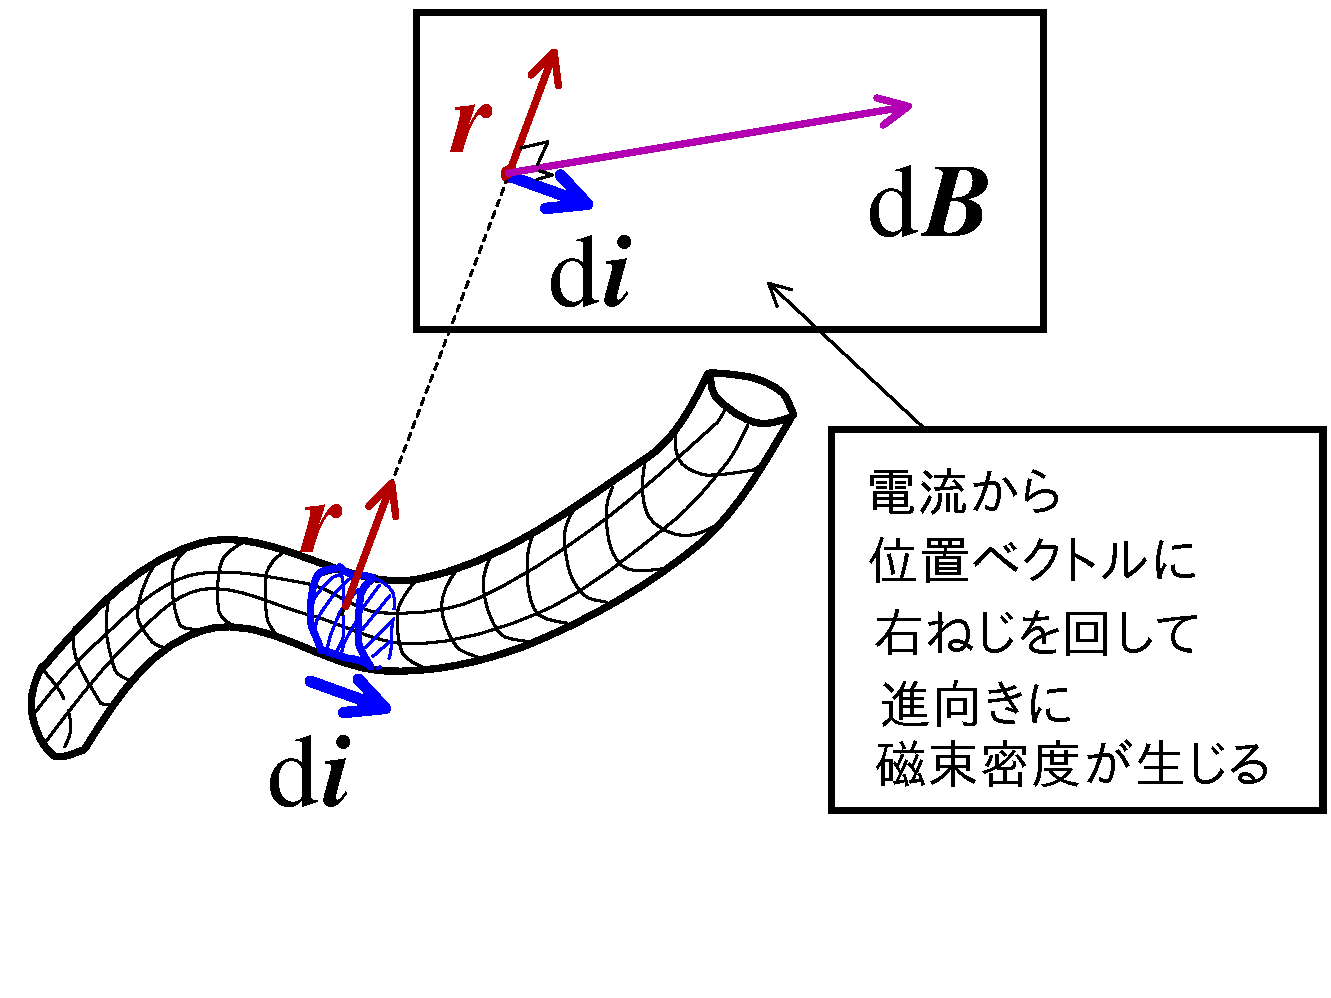
\includegraphics[keepaspectratio, width=7.2cm, height=5.79cm, clip]{biot_savart_1.pdf}
                    \caption{ビオ$=$サバールの法則}
                    \label{fig:biot_savart_1}
                \end{center}
            \end{figure}

    \subsection{点電荷の場合}
    最後に,電気量 $q$ をもつ点電荷に関する表示もしておこう.
    最初に示した式(\ref{Bior=savart'slow1})を思い起こそう.
        \begin{align*}
            \bB(\br)
            &=\frac{\mu_{0}|\bI|}{4\pi}
             \int_{\Gamma}\frac{\bt_{I}(\br')\times
                     (\br-\br')
                   }{|\br-\br'|^{3}}\df s' \\
            &=\frac{\mu_{0}}{4\pi}
             \int_{\Gamma}\frac{\bt_{I}(\br')\times
                     (\br-\br')
                    }{|\br-\br'|^{3}}|\bI|\df s'  \\
            \frac{\df \bB(\br)}{\df s'}
            &=\frac{\mu_{0}}{4\pi}
             \frac{\bt_{I}(\br')\times
                     (\br-\br')
                    }{|\br-\br'|^{3}}|\bI|  \\
            \df \bB(\br)
            &=\frac{\mu_{0}}{4\pi}
             \frac{\bt_{I}(\br')\times
                     (\br-\br')
                    }{|\br-\br'|^{3}}|\bI| \df s'  \\
            &=\frac{\mu_{0}}{4\pi}
             \frac{|\bI|\df s' \bt_{I}(\br')\times
                     (\br-\br')
                    }{|\br-\br'|^{3}}   \\
            &=\frac{\mu_{0}}{4\pi}|\bI|\df s' \bt_{I}(\br')\times
             \frac{(\br-\br')}{|\br-\br'|^{3}}
        \end{align*}

        ここで,\textbf{電流素片} という概念を導入しよう.
        上式の $|\bI|\df s' \bt_{I}(\br')$ に
        注目する.$\df s'$ は導線の微小な長さであるから,
        $|\bI|\df s' \bt_{I}(\br')$ という量は
        電流の微小な一部分であとみなせる.
        この $|\bI|\df s' \bt_{I}(\br')$ のことを電流素片と
        よぶことにしよう
            \footnote{
                教科書によっては,\textbf{電流要素} と表現されることもある.
            }.
        \begin{figure}[hbt]
            \begin{center}
                \includegraphicsdefault{dennryu_sohenn.pdf}
                \caption{電流素片 $|\bI|\df s \bt_{I}(\br)$}
                \label{fig:dennryu_sohenn}
            \end{center}
        \end{figure}


        電流素片 $|\bI| \df s'$ はその極限は,ひとつの点電荷の移動であると
        考えられる.点電荷の電気量を $q$,その速度を $\bv$ とすると,
        \begin{align*}
            |\bI| \df s' = q\bv.
        \end{align*}
        つまり,速度をもった点電荷が作る磁束密度 $\bB(\br)$ は
            \footnote{
                ここで,改めて,$\df \bB(\br)$ を $\bB(\br)$ に表示を置き換える.
                $\df \bB(\br)$ は電流の微小部分の作る磁束密度というイメージであったが,
                今考えている点電荷のつくる磁束密度であるので,それを $\bB(\br)$ と
                表現しても間違いではないだろう.いや,むしろこのように書き換えたほうが,
                式を自然な形にさせることができると思う.
            },
        \begin{align*}
            \bB(\br)
            &=\frac{\mu_{0}}{4\pi}q\bv \times
             \frac{\br-\br'}{|\br-\br'|^{3}}.
        \end{align*}
        \begin{myshadebox}{ビオ$=$サバールの法則(点電荷表示)}
            速度 $\bv$ で運動する,電気量 $q$ をもつ電荷は,次式で表される
            磁束密度 $\bB(\br)$ をその周囲に発生させる.
            \begin{align}
                \bB(\br)
                 &=\frac{\mu_{0}}{4\pi}q\bv \times
                  \frac{\br-\br'}{|\br-\br'|^{3}}.
            \end{align}
        \end{myshadebox}



%===================================================================================================
%  Chapter : 電磁気力(ローレンツ力)
%  説明    : 電磁気学的な力(電磁気力;ローレンツ力)の概念を導入する
%===================================================================================================
\chapter{電磁気力(ローレンツ力)}
%   %-----------------------------------------------------------------------------------------------
%   %  Input
%   %    File Name : PhysNote_EM_1st_LorentzForce.tex
%   %    説明      : クーロン力と磁束密度に関するローレンツ力を統合し,電磁気力を定める.
%   %-----------------------------------------------------------------------------------------------
        
%======================================================================
%  Section
%======================================================================
\section{ローレンツ力(電磁気力)}
    クーロン力 $\bF_{\mathrm{Coulomb}}$ と
    磁束密度に関するローレンツ力 $\bF_{\mathrm{Lorentz}}$ に
    よって,電気的な力と電荷が磁束密度より受ける力を記述する方法を得た.
        \begin{align*}
               & \bF_{\mathrm{Coulomb}} = q\bE. \\
                &\bF_{\mathrm{Lorentz}} = q\bv\times\bB.
        \end{align*}

    ところで,これまで「磁束密度に関するローレンツ力」という表現をしきりに使用
    してきた.わざわざ“磁束密度に関する”なんていう但し書きのような言い回しを
    してきたのには,理由がある.それは,単に \textbf{ローレンツ力} といった
    とき,それは
        \begin{align*}
            \bF &= \bF_{\mathrm{Coulomb}} + \bF_{\mathrm{Lorentz}} \\
                &= q(\bE + \bv\times\bB)
        \end{align*}
    のようなクーロン力と磁束密度に関するローレンツ力の和を指すからである
        \footnote{
            ちなみに,“電場に関するローレンツ力”なんてものは存在しない.ただ,
            磁束密度 $\bB$ や電荷 $q$ が0のときのような場合のローレンツ力は,
            クーロン力と等しくなり,電場に関するローレンツ力といっても間違い
            ではないとは思うが,一般的に通用する語彙ではない.
        }.
    \begin{myshadebox}{ローレンツ力}
        ある空間に電場 $\bE$ と磁束密度 $\bB$ が存在するとき,
        電気量 $q$ をもつ点電荷(以下,電荷 $q$ と書く)が
        速度 $\bv$ で運動しているならば,この電荷 $q$ には
        次式で示す \textbf{ローレンツ力} $\bF$ を受ける.
        \begin{align}
            \bF = q(\bE + \bv\times\bB)
        \end{align}
    \end{myshadebox}

\section{ローレンツ力と観測者}
        このローレンツ力は,不思議な力である.というのも,この力は
        観測者と電荷との相対的な速度 $\bv$ によっているからである.
        同じ電荷を観測していても,観測者によって電荷との相対速度
        が異なるのであれば,ローレンツ力の向きや大きさは,観測者ごとに
        異なったものとなる.なんとも不思議なことであるが,
        相対性理論を受け入れれば,何の不思議なことではなくなる.
        しかし,ここでは電磁気学を学ぶことが目標であるので,
        とりあえず,この不思議さは棚上げにしておき,話を
        先に進めることにしよう.


    \begin{memo}{電荷自身から発する磁束密度}
        電荷が磁束密度中を運動するときには,それにより磁束密度
        に関するローレンツ力を受け,速度の方向が変化してしまう.
        しかし,あとで述べるとおり,アンペールの法則によれば,
        磁束密度の発生源は電流である
            \footnote{
                アンペールの法則(※1)は
                次式で表現される.
                \begin{align*}
                    \drot\bB =  \mu_{0}\left(
                                    \bi + \frac{\rd \bE}{\rd t}
                                \right)
                \end{align*}
                言葉で表現すれば,大雑把に,
                \begin{align*}
                    \mbox{回転する磁束密度} = \mbox{電流} + \mbox{時間変動する電場}
                \end{align*}
                という感じになろう.詳しいことは,後に考える.

                (※1)正確には「アンペール$=$マクスウェルの法則」というべきだ.
            }.

        電荷が速度をもっていれば,
        それは電流と同一視できることになり,つまり,その物体自
        身がその周囲に磁束密度を生じさせていることになる.

        たしかに,はじめに考えたように,速度をもった電荷は,自身が
        発している磁束密度とは発生源が異なる磁束密度の影響をうけて,
        その方向が変化する.しかし一方で,電荷から発している磁束密度
        は,その周囲の磁束密度に影響を与えていることも事実である.

        そうであるとき,その影響はどの程度なのだろうか.それは,
        磁束密度に関するローレンツ力が $q\bv\times\bB$ と表される
        ことから,電荷の電気量 $q$ と速度 $\bv$ の大きさに依存している
        ことは明らかである.

        つまり,電荷を除いた状態での純粋な空間の磁束密度を $\bB_{\mathrm{pure}}$ と
        し,電荷から生じる磁束密度を $\bB_{\mathrm{q}}$ としたならば,電荷が
        存在する場合の正味の空間の磁束密度 $\bB$ は
            \begin{align*}
                \bB = \bB_{\mathrm{pure}} + \bB_{\mathrm{q}} \\
            \end{align*}
        である.だから,電荷が受ける磁束密度に対するローレンツ力は,
            \begin{align*}
                \bF &= q \bv \times \bB \\
                    &= q \bv \times (\bB_{\mathrm{pure}} + \bB_{\mathrm{q}}) \\
                    &= q \bv \times  \bB_{\mathrm{pure}} + q \bv \times \bB_{\mathrm{q}} \\
                \therefore\quad
                \bF &= q \bv \times  \bB_{\mathrm{pure}} + q \bv \times \bB_{\mathrm{q}}
            \end{align*}
        となり,$q \bv \times \bB_{\mathrm{q}}$ という分だけ,周囲の磁束密度を
        変化させ,それが自分の受ける磁束密度に対するローレンツ力に跳ね返ってくる.

        ここで気になるのは,$\bB_{\mathrm{q}}$ である.これは運動している電荷から
        発している磁束密度である.
        大きさはどのくらいで,どの方向に磁束密度は生じているのだろうか.
        これはビオ$=$サバールの法則から,位置 $\br$ に発生させる磁束密度 $\bB(\br)$ は
            \begin{align*}
                \bB_{\mathrm{q}}(\br) =
                \frac{\mu_{0}}{4\pi}q\bv \times
                \frac{\br-\br'}{|\br-\br'|^{3}}.
            \end{align*}
       と計算される.ここに,$\br'$ は磁束密度を観測する固定点である.
       とすれば,電荷が受ける磁束密度に対するローレンツ力は次のようになる.
            \begin{align*}
                \bF &= q \bv \times \bB_{\mathrm{pure}} + q \bv \times
                \left(
                    \frac{\mu_{0}}{4\pi}q\bv \times \frac{\br-\br'}{|\br-\br'|^{3}}
                \right) \\
                &= q \bv \times \bB_{\mathrm{pure}} + \frac{\mu_{0}}{4\pi}
                \left( q^{2} \bv \times \bv \times \frac{\br-\br'}{|\br-\br'|^{3}}
                \right).
            \end{align*}
        結果が見えてきた.ここで,ベクトル解析の公式,任意のベクトル $\bX$ に対して,
        $\bX \times \bX = \bzero$ を思い起こせば,
            \begin{align*}
                \bF &= q \bv \times \bB_{\mathrm{pure}} + \frac{\mu_{0}}{4\pi}
                \left(
                    q^{2} \bzero \times \frac{\br-\br'}{|\br-\br'|^{3}}.
                \right)\\
                &= q \bv \times \bB_{\mathrm{pure}} + \bzero \\
                \therefore\quad
                \bF &= q \bv \times \bB_{\mathrm{pure}}.
            \end{align*}
        この式の意味するところは,明白である.
        運動する電荷から発している磁束密度より受けるローレンツ力は,
        電荷自身に対して影響を及ぼさない,ということである.
        考えて見れば,簡単にイメージができることである.速度をもつ
        電荷がその周囲につくる磁束密度 $\bB_{\mathrm{q}}$ は,その速度に対して垂直な方向に
        生じる.なので,$\bB_{\mathrm{q}}$ は運動する電荷に対して,
        なんのエネルギーも与えないのだ
            \footnote{
                仕事の定義 $W = \bF \cdot \br$ を思い起こそう.物体に仕事を
                すると,それはエネルギーとして蓄えられるのだが,垂直成分は
                それに寄与しない.なぜなら,
                    \begin{equation*}
                        \bF \cdot \br = |\bF||\br| \cos \theta =  |\bF||\br| \cos(\pi/2) = 0.
                    \end{equation*}
            }.
    \end{memo}


%===================================================================================================
%  Chapter : マクスウェル方程式概観
%  説明    : マクスウェル方程式を帰納的に導く
%===================================================================================================
\chapter{マクスウェル方程式概観}
%   %-----------------------------------------------------------------------------------------------
%   %  Input
%   %    File Name : PhysNote_EM_1st_MaxEqImage.tex
%   %    説明      : マクスウェル方程式について,
%   %                その意味するところを言葉で大まかにイメージする
%   %-----------------------------------------------------------------------------------------------
        %   %==========================================================================
%   %  Section
%   %==========================================================================
    \section{4つの基本法則}\label{sec:4fundlaw}
    \begin{mycomment}
        ここでは,真空中の電磁気現象を想定する.言い換えれば,
        物質内のおける電場や磁束密度については想定していない.
        物質が存在する場合の理論は複雑になり,最初に学習する
        際には,理論の骨格を捉えにくいものである.理論の筋道を
        明確に捉えるために,真空中であるという制約を与える.
    \end{mycomment}

%       %======================================================================
%       %  SubSection
%       %======================================================================
        \subsection{はじめに}\label{subseq:4fundlaw_Hajimeni}
        電磁気的現象は4つの基本法則によって説明できる.ニュートン力学
        で言うところの,ニュートンの運動の3法則に対応する部分である.ついでに,
        それに対する方程式も記述しておこう.
            \begin{enumerate}
                \item 電場に対するガウス
                    \footnote{
                        Johann Carl Friedrich Gauss(Gau\ss)(1777--1855, ドイツ)
                        :ドイツの数学者,物理学者.整数や代数についての研究,曲
                        面論などに代表される幾何学の研究が有名である.近代数学の
                        大部分にその業績があり,19世紀最大の数学者とも言われる.
                        また,cgs単位系の「ガウス[G]」は磁気の単位として使われ
                        ている.そのほかにも,「ガウス記号(整数論)」,「ガウス
                        平面(複素関数論)」,「ガウス分布(誤差論)」など彼の名
                        がつけられた概念は多い.
                    }
                    の法則
                    \begin{align}
                        \ddiv \bE = \frac{1}{\varepsilon_{0}}\rho.
                    \end{align}
                \item 磁束密度に対するガウスの法則
                    \begin{align}
                        \ddiv \bB = 0.
                    \end{align}
                \item アンペール
                    =マクスウェル
                    \footnote{
                        James Clerk Maxwell(1831--1879, イギリス):古典電磁気学
                        の理論体系を築いた.この理論より電磁波の予言を行い,ヘル
                        ツ(Heinrich Rudolf Hertz, 1857--1894, ドイツ)らによって
                        実験的に実証された.

                        電磁気学的な自然現象は,4つの法則を基本法則とすることで,
                        説明のつく現象であると提唱する
                        (1865年;A dynamical theory of the electromagnetic field).
                        その後,マクスウェルは,1873年に,電磁気学を体系的に纏めた教科書を
                        出版し,電磁気学を確立させた
                        (1873年;A treatse on electricity and magnetism).
                        この教科書は,電磁気学におけるプリンキピアであると言われるようだ
                        (褒め言葉であると同時に,難解であるという意味も込められているらしい).

                        また,統計物理学の基本的な考え方である,気体分子運動論にかんする
                        研究も行なっている.「マクスウェル分布(マクスウェル--ボルツマン分布)」
                        としても,その名前を残している.これは今日の統計物理学の基礎をなすもの
                        である.

                        また,マクスウェルはキャベンディッシュ(\ref{sec:EM_ObjPreMsg}節の脚注を参照)
                        の仕事を世の中に紹介している.そして,当時新しく設けられた,
                        「キャベンディッシュ研究所」の実験物理学の教授(初代所長)として働いている.
                        なおこの研究所は,上に紹介したキャベンディッシュ(Henry Cavendish)の子孫
                        に当たる,デヴォンシャー第7大公爵が出資して作られた,
                        ケンブリッジ大学の実験物理学施設である.

                        片仮名表記される場合,「マックスウェル」とかかれることもある.

                        (参考1)太田 浩一,『マクスウェルの渦 アインシュタインの時計 現代物理学の源流』,
                        東京大学出版会

                        (参考2)William H.Cropper,『物理学天才外伝』, 講談社(ブルーバックス)
                    }
                    の法則
                    \begin{align}
                        \drot \bB = \mu_{0}\bi + \varepsilon_{0}\mu_{0}\frac{\rd \bE}{\rd t}.
                    \end{align}
                \item ファラデー
                    \footnote{
                        Michael Faraday(1791--1867, イギリス):電磁誘導の発見,
                        電気力線,磁力線の提唱(電磁気現象の近接作用の考え)など,
                        電磁気学に大きい貢献をする.また,化学者としての活躍も有名
                        であり,電気分解の法則の発見がその例である.コンデンサの容
                        量の単位「ファラド[F]」や,ファラデー定数などは,彼の名に
                        ちなんだものである.
                    }
                    の電磁誘導の法則
                    \begin{align}
                        \drot \bE = - \frac{\rd \bB}{\rd t}.
                    \end{align}
            \end{enumerate}

        以下では,これら4つの法則の内容をざっくりと見ていこう.その実験的根拠等の
        細かいことは,次章以降で考えることにする.ここでは,電磁気学は4つの基
        本法則から構成されているのだということを理解してもらいたい.
        各法則が意味する現象の詳細は,後で,それぞれ章を立てて説明する.

        もう一度注意しておこう.先のコメントの部分にも書いたが,以降で想定するのは,
        すべて,真空中で起こる電磁気現象である.物質を含む場合については,また別に
        議論することとにしたい.


%       %======================================================================
%       %  SubSection
%       %======================================================================
        \subsection{電場に対するガウスの法則}
        電場に対するガウスの法則は,電場の発生と消滅に関する法則である.内容は次
        の通りである.
            \\
            \begin{itembox}[l]{\textbf{電場に対するガウスの法則}}
                電場の\textbf{発生源}は\textbf{正に帯電した電荷}である.また,電
                場の\textbf{消滅源}は\textbf{負に帯電した電荷}である.そして,電
                場の発生と消滅は電荷においてのみ起こり,これ以外では起こらない.
            \end{itembox}
            \\

        この法則の意味するところは,電場の発生と消滅の原因は電荷にあることの主張
        である.正に帯電したから電荷から発生した電場は,負に帯電した電荷に吸収(
        消滅)するのである.そして,電場の発生,消滅は電荷以外では起こりえない.
               \begin{figure}[hbt]
                    \begin{tabular}{cc}
                        \begin{minipage}{0.5\hsize}
                            \begin{center}
                                \includegraphicsdouble{GaussLowImage_01.pdf}

                                (A) 正電荷より電場発生
                            \end{center}
                        \end{minipage}
                        \begin{minipage}{0.5\hsize}
                            \begin{center}
                                \includegraphicsdouble{GaussLowImage_02.pdf}

                                (B) 負電荷で電場消滅
                            \end{center}
                        \end{minipage}
                    \end{tabular}
                                \caption{電場に対するガウスの法則}
                                \label{fig:GaussLowImage}
                \end{figure}


%       %======================================================================
%       %  SubSection
%       %======================================================================
        \subsection{磁束密度に対するガウスの法則}
        磁束密度に対するガウスの法則は,磁束密度の発生と消滅に関する法則である.
        内容は次の通りである.
            \\
            \begin{itembox}[l]{\textbf{磁束密度に対するガウスの法則}}
                磁束密度の\textbf{発生源},\textbf{消滅源}は存在しない.
            \end{itembox}
            \\

        磁束密度がある点から生じて,他の点に吸収されるようなことは起こりえない
        ことを,この法則は主張する.つまり,電場の発生源とはる電荷に対応するよう
        な,言わば磁荷は存在しないことを意味する.
                \begin{figure}[hbt]
                    \begin{center}
                        \includegraphicsdefault{GaussLowBImage_01.pdf}
                        \caption{磁束密度に対するガウスの法則}
                        \label{fig:GaussLowBImage_01}
                    \end{center}
                \end{figure}

%       %======================================================================
%       %  SubSection
%       %======================================================================
        \subsection{ファラデーの電磁誘導の法則}
        ファラデーの電磁誘導の法則は,磁束密度の時間的な変化と電場の関係に関する
        法則である.内容は次の通りである.
           \\
           \begin{itembox}[l]{\textbf{ファラデーの電磁誘導の法則}}
               磁束密度が時間的に変化すると,その周囲には回転する電場が発生する.
           \end{itembox}
           \\

        磁束密度とは磁界のことだから,磁界の変化が回転する電場を発生させることに
        なる.具体的な例で考える.磁石は磁界を発生させていることは,中学生なら
        ば誰でもでも知っている.とすれば,磁界が変化する状況を作るには,磁石を手
        で持って振ればよい.ファラデーの電磁誘導の法則の法則は,この手で振ってい
        る磁石の周りに,電場が生じていると主張しているのである.
                \begin{figure}[hbt]
                    \begin{center}
                        \includegraphicsdefault{FaradayLowImage_01.pdf}
                        \caption{ファラデーの電磁誘導の法則}
                        \label{fig:FaradayLowImage_01}
                    \end{center}
                \end{figure}


%       %======================================================================
%       %  SubSection
%       %======================================================================
        \subsection{アンペール$=$マクスウェルの法則}
        アンペール$=$マクスウェルの法則は,電場の時間的な変化と磁束密度に関する法
        則である.内容は次の通りである.
            \\
            \begin{itembox}[l]{\textbf{アンペール$=$マクスウェルの法則}}
                電流の周りには,この電流を取り囲むように回転する磁束密度が生じる.ま
                たこれに加えて電場の状態が時間的に変化すると,その周囲には回転す
                る磁束密度が発生する.
            \end{itembox}
            \\

        電流が流れていると,その周りには磁界が発生しているということは,おそらく
        中学で習うはずだ.この法則では,それに加えて,時間的に変化する電場も,回
        転する磁束密度を作ることを主張している.
                \begin{figure}[hbt]
                    \begin{tabular}{cc}
                        \begin{minipage}{0.5\hsize}
                            \begin{center}
                                \includegraphicsdouble{AMLaw_Image00.pdf}

                                (A) 電流による磁場
                            \end{center}
                        \end{minipage}
                        \begin{minipage}{0.5\hsize}
                            \begin{center}
                                \includegraphicsdouble{AMLaw_Image01.pdf}

                                (B) 電場の時間変化による磁場
                            \end{center}
                        \end{minipage}
                    \end{tabular}
                        \caption{電流と時間変化する電場は,その周囲に回転する磁場を生じる}
                        \label{fig:AMLaw_Image00}
                \end{figure}

%   %==========================================================================
%   %  Section
%   %==========================================================================
    \section{マクスウェル方程式を見てみよう}
        \begin{mycomment}
            この節では,マクスウェル方程式を実際に見てみよう.
            だたし,その式をイメージとして捉え,意味すること
            を重視する.数式の本来の性質等は,各法則毎に詳しく
            調べることにし,ここでは数式の形に慣れることが目的
            である.徐々にマクスウェル方程式に馴染んで行こう.
        \end{mycomment}

%       %======================================================================
%       %  SubSection
%       %======================================================================
        \subsection{「マクスウェル方程式」とは}
        \begin{mycomment}
            まずは,「マクスウェル方程式」と言われる式について説明する.
            実は,マクスウェル方程式と言われてはいるが,マクスウェルがその
            方程式を発見したのではない.勘違いを起こしてしまいがちだが,
            マクスウェルが発見したという意味での,方程式は存在しないのである.
            ではどういうことかというと,言うなれば,
               “マクスウェルが提唱した,電磁気の公理的な4つの連立方程式”
            がマクスウェル方程式と呼ばれるものである.
        \end{mycomment}

%           %==================================================================
%           %  SubsubSection
%           %==================================================================
            \subsubsection{マクスウェルが電磁気学を確立する}
            電磁気的な自然現象には,冬場に発生する静電気や,より身近なものとして,
            磁石がある.携帯電話や無線LANも電磁気現象(電磁波)を利用した装置である.
            電磁気的な現象は,一見すると,その発生機構が複雑であるように感じてしまう.
            たしかに,マクスウェルにより指摘される以前では,電磁気現象は複雑であると
            感じることだったろう.しかし,今では,電磁気現象は,たった4つの法則を認め
            るだけで,説明ができることが分かっている.これを指摘した人物
            こそマクスウェルである.

            マクスウェルの提唱した4つの法則は,それ以前に先人
                \footnote{
                    例えば,アンペール,クーロンなどがいる.
                }
            により発見されていた自然現象をピックアップしたものであり,つまり,
            マクスウェル自身が4つの法則を発見したわけではない.マクスウェルの偉大なところ
            は,それまで煩雑としていた電磁気現象に関する実験結果(実験法則)を,体系化した
            ことにある.それまでには,色々な電磁気学の実験が行われて,その実験結果も
            多様にあったはずである.マクスウェルは,この煩雑な実験結果は,4つの自然現象
            を受け入れることで,すべてが上手く(数学的に)説明できることを示唆した.

%           %==================================================================
%           %  SubsubSection
%           %==================================================================
            \subsubsection{数式で表現してこそ,基本法則と言える}
            マクスウェルが基本法則として取り上げた4つの実験結果については,定性的には,
            上で紹介しと通りである(\ref{sec:4fundlaw}節参照).しかし,これらの法則は,
            数式により表現してこそ,意味を成す
                \footnote{
                    物理現象を説明するには,数式によりそれを表現すべきだ.
                    数式で表されて,初めて,詳細な推論や論理的思考が可能になるからだ.
                    数式を用いずに,言葉で表現しても論理的推論が不可能というわけではないが,
                    考えにくいし,論理もわかりにくくなる.数式で表現できれば,論理的
                    推論もしやすくなるし,論旨もわかりやすくなる.
                    不慣れな数式を扱うことが億劫かもしれなが,ここは少々なれるまで我慢
                    してもらいたい.物理学は数式を扱う学問なので,数式に慣れることは大事だ.
                    4つの法則で電磁気学現象を説明できるといったのは,各法則を方程式
                    で表したときに,電磁気現象が4つの方程式から数学的演算により,
                    論理的必然性をもった結果として導かれることをいう.
                }.
            そこで,次に,4つの基本法則を表す数式を紹介する.ただし,その数式に深入り
            することはせず,そのイメージを捉えることを第一の目的としたい.より詳しいことは,
            次章以降で考える
                \footnote{
                    実は,以下に説明する4つの方程式の理解こそが,初めて電磁気学を学ぶ際の
                    目標なのである.つまり,ここでは,その最終目標を先回りして紹介すること
                    になる.これは,学習の目標を明確にすることを考えてのことである.目標が
                    明確になれば,学習の際の不安(何をしているのかが分からないなど)も,少
                    しは解消されることと思う.
                }.

%           %==================================================================
%           %  SubsubSection
%           %==================================================================
            \subsubsection{マクスウェル方程式の2種類の表現}
            マクスウェル方程式は4つであるが,実は,その表現方法が2種類があり,
            微分を使って表現したものが \textbf{微分形},
            積分を使って表現したものが \textbf{積分形} と言われる.ここでは,
            この2種類の表現方法を紹介する.微分形と積分形の違いは,視点の違いである.
            現実に起こっている現象を肌で感じる場合には,積分形の方程式を用いる.
            そのため,工学の分野では,積分形を使うことのほうが多いと思う.これに対し,
            微分形で記述されたものは,現象を局所的に見た場合に使われる.微分形は
            理論的考察を行う場合に使うことが多い.もちろん,積分形で表されようが,
            微分形で表されようが,その式は全く等価である(当たり前のはずだが,念のために).


%       %======================================================================
%       %  SubSection
%       %======================================================================
        \subsection{約束:独立変数の記述の省略}
                マクスウェル方程式は,位置 $\br$ と時間 $t$ の4つの独立変数を
                含む関数の間に成り立つ式であるが,この独立変数をいちいち明記
                していたら,式が煩雑になり見難くなっていしまう.そこで,
                以下のように,独立変数を省略して記述する.
                すなわち,
                電場 $\bE$,磁束密度 $\bB$,電流密度 $\bi$,電荷密度 $\rho$ であり,
                その意味は次式の通り.
                    \begin{align*}
                        \bE  &= \bE(\br,\,t) \\
                        \bB  &= \bB(\br,\,t) \\
                        \bi  &= \bi(\br,\,t) \\
                        \rho &= \rho(\br,\,t)
                    \end{align*}
                また,$\varepsilon_{0}$,$\mu_{0}$ は,それぞれ,真空中の誘電率,透磁率と言われる,
                スカラー量で,単なる定数である(位置と時間の関数ではない).

                ついでに,他の記号も説明する.
                任意の閉曲面を $S$ で表現する.また,$S$ で囲まれた内部の領域全体を $\Omega_{S}$ と
                書く.閉曲面の微小部分は $\df S$ であり,
                $\df S$ の単位法線ベクトルは $\bn:=\bn(\br,\,t)$ で表現する.
                また,$l$ は任意の閉経路(ループしている経路,輪状の経路のこと)である.そして,$S_{l}$ というのは,
                閉経路 $l$ を縁とする開曲面を表す.そして,閉経路 $l$ の単位接線ベクトルを $\bt:=\bt(\br,\,t)$ と
                表現する.

                くどいかもしれないが,演算に関する記述方法の説明もしておこう.
                $\sint_{S} X\df S$ は,関数 $X$ を,$S$ に対して面積分を行うことを意味する.また,
                $\vint_{\Omega_{S}} X \df V$ は,関数 $X$ を,$S$ の内側の全領域 $\Omega_{S}$ に
                対して体積分を行うことを意味する.

%       %======================================================================
%       %  SubSection
%       %======================================================================
        \subsection{マクスウェル方程式(微分形)}
        \begin{mycomment}
            上では,現実に起こっている法則のイメージを説明したが,
            ここではもう一歩先に進んで数式を眺めてみよう.この節では,
            微分形のマクスウェル方程式を確認する.積分形も,後で確認する.
            何度も言うが,
            数式そのものを理解することが目的ではなく,数式のイメージを
            持つことが目的である.数式の詳細は後で述べる.ここではとにかく,
            求めるべきマクスウェル方程式がどのようなものかを,感覚的に
            把握してもらいたい.
        \end{mycomment}
%           %==================================================================
%           %  SubsubSection
%           %==================================================================
            \subsubsection{電場に対するガウスの法則の式:微分形}
            \begin{mysmallsec}{数式}
                電場に対するガウスの法則の,微分形の式は次式の通り.
                \begin{align}
                    \ddiv \bE = \frac{1}{\varepsilon_{0}}\rho.
                \end{align}
            \end{mysmallsec}

            \begin{mysmallsec}{法則のイメージ}
                電場の発生あるいは消滅は,電荷の存在する場所で生じる.また,言い換えれば,
                ある場所において,電場が発生あるいは消滅していることと,その場所に電荷が
                存在することは,同じ意味をなす.

                ベクトル $\bE$ は電場で,その前に書かれている $\ddiv$ は,
                divergence(発散) を意味する.なので,左辺 $\ddiv \bE$ は電場の発散を表す.
                右辺の$\rho$ は電荷密度
                    \footnote{
                        1/$\varepsilon_{0}$ がかかっているが,単なる比例定数である.
                        これは単位系としてSI単位を採用していることによって現れた定数
                        であり,式の表す物理的イメージにはあまり関係がないと思って良い.
                    }
                であり,電荷密度の存在が表されている.
                電場の発散と電荷密度が等号で結ぶことによって意味されることは,
                「電荷密度が存在すれば,その周囲には電場の発散が生じる」ということである.
                更にその逆もいうことができて,「電場の発散の原因は電荷密度である」ということも
                できる.
                電場の発生あるいは消滅は,電荷の存在しない場所では,絶対に発生しない.
            \end{mysmallsec}

                \begin{figure}[hbt]
                    \begin{center}
                        \includegraphicsdefault{GaussLowEImage_03.pdf}
                        \caption{電場は電荷より生じる}
                        \label{fig:GaussLowEImage_03}
                    \end{center}
                \end{figure}

%           %==================================================================
%           %  SubsubSection
%           %==================================================================
            \subsubsection{磁束密度に対するガウスの法則の式:微分形}
            \begin{mysmallsec}{数式}
                磁束密度に対するガウスの法則の,微分形の式は次式の通り.
                \begin{align}
                    \ddiv \bB = 0.
                \end{align}
            \end{mysmallsec}

            \begin{mysmallsec}{法則のイメージ}
                この式は,磁束密度はどこからも湧き出しがないことを表現している.
                見方を変えれば,ある部分で湧き出す磁束密度の量と,その部分で消滅する
                磁束密度の量が等しいから,正味として湧き出しがないとみなされる.

                つまり,磁束密度の発生場所を特定することはできないということである.
                こういう言い方すると,“磁束密度は存在して,その発生原因は電流にあることを,
                先に説明している.つまり,発生している場所を示すことができるではないか”と
                いう疑問を持たれてしまうかもしれない
                    \footnote{
                        少なくとも,私はそう思った.
                    }.
                しかし,これは言葉の意味の捉え方(あるいは記述の仕方)の問題であり,
                磁束密度の存在場所が特定できないことを言っているのではない.この法則は
                ,あくまでも,発生源を特定することができないということであり,発生して
                いる場所を示せないということではない.現に,磁石の周囲には磁束密度が存在
                していることは,すでに知っていることである.たしかに,磁石から磁束密度が
                湧き出していると考えても,間違いではないが,この法則の言っている「湧き出し」とは
                意味がことなる.先にも書いたとおり,ここで言う「湧き出し」とは,磁束密度の
                生じる量と消滅する量の,“正味の湧き出し”ということである.この正味の湧き出しが
                0であるというとは,この世界のどの場所を見ても磁束密度の正味の湧き出しがないという
                ことを意味しているのである.この「正味の」という部分に,注意すべきだ.
            \end{mysmallsec}

                \begin{figure}[hbt]
                    \begin{center}
                        \includegraphicsdefault{GaussLowBImage_02.pdf}
                        \caption{磁束密度の湧き出しはない}
                        \label{fig:GaussLowBImage_02}
                    \end{center}
                \end{figure}


%           %==================================================================
%           %  SubsubSection
%           %==================================================================
            \subsubsection{アンペール$=$マクスウェルの法則の式:微分形}
            \begin{mysmallsec}{数式}
                アンペール$=$マクスウェルの法則の式の,微分形の式は次式の通り.
                \begin{align}
                    \drot \bB = \mu_{0}\bi + \varepsilon_{0}\mu_{0}\frac{\rd \bE}{\rd t}.
                \end{align}
            \end{mysmallsec}

            \begin{mysmallsec}{法則のイメージ}
                右辺に項が2つあるが,これらはそれぞれ,意味することが異なる.
                右辺の第一項は,電流が磁場を作るということを主張するものである.
                これは,アンペールの法則とよばれる
                    \footnote{
                        アンペールの法則とは,上式の第二項が常に0である場合のことである.
                        すなわち,次式がアンペールの法則を表す式である.
                            \begin{align}
                                \drot \bB = \mu_{0}\bi.
                            \end{align}
                        アンペールの法則の意味するところは,式を見れば明らかである.
                        口うるさく意味を説明すれば,
                        「回転している磁束密度が存在するということは,その内側の領域に
                        電流が生じていることを意味する」ということだ.
                    }.
                そして,第二項が意味するのが,
                \textbf{変位電流} という概念である.詳細は後述するが,ここでは,
                おおよそのイメージとして,電場の時間変化がその周囲に磁束密度を
                生じさせる,と解釈して欲しい
                    \footnote{
                        式をそのまま言葉にしただけである.その真意の程は後の記述を
                        参照.
                    }.

                なぜ,「変位電流」を導入する必要があるのかというと,単なるアンペールの法則が
                電荷保存則に矛盾してしまうからである.つまり,アンペールの法則と電荷保存則の
                どちらかが,間違っている(不完全である)可能性があるということである
                    \footnote{
                        あるいは,どちらとも間違いなのかもしれない.しかしこの可能性は,
                        あとに記述する,マクスウェルの修正によってなくなる.
                    }.
                マクスウェルによる回答は,アンペールの法則が不完全である,ということだった.
                そして,マクスウェルはアンペールの法則を完全な形にすべく,「変位電流」という
                新しい概念を考案し,アンペールの法則にそれを組み込むことで,電荷保存則との
                矛盾を解消したのである.

                あとに分かることだが,この変位電流は,ファラデーが発見する電磁誘導の法則
                に対をなす現象である,と見ることもできる.この変位電流と電磁誘導とにより,
                電磁波という現象が起こるのである.電磁波についても,後ほど考えることにしたい
                    \footnote{
                        マクスウェル方程式の偉大さの一つは,電磁波の存在を予言したことである.
                    }.

                もう一度改めて,この法則の内容を確認しておこう.電流はその周囲に磁束密度を
                発生させる.さらに,それに加えて,電場の時間変化が起きた際にも,その電場の
                変化にともなって,その周囲に,磁束密度が生じるのである.
            \end{mysmallsec}

                \begin{figure}[hbt]
                    \begin{tabular}{cc}
                        \begin{minipage}{0.5\hsize}
                            \begin{center}
                                \includegraphicsdouble{dennryu_to_jisokumitudo.pdf}

                                (A) 電流による磁場
                            \end{center}
                        \end{minipage}
                        \begin{minipage}{0.5\hsize}
                            \begin{center}
                                \includegraphicsdouble{hennnidenryu_to_jisokumitudo.pdf}

                                (B) 変位電流による磁場
                            \end{center}
                        \end{minipage}
                    \end{tabular}
                        \caption{電流,変位電流と磁束密度の関係}
                        \label{fig:I_i_B}
                \end{figure}


%           %==================================================================
%           %  SubsubSection
%           %==================================================================
            \subsubsection{ファラデーの電磁誘導の法則の式:微分形}
            \begin{mysmallsec}{数式}
                ファラデーの電磁誘導の法則の式の,微分形の式は次式の通り.
                \begin{align}
                    \drot \bE = - \frac{\rd \bB}{\rd t}.
                \end{align}
            \end{mysmallsec}

            \begin{mysmallsec}{法則のイメージ}
                左辺は回転する電場を表している.右辺は負の符号がついて入るが,
                磁束密度の時間変化が記述されている.渦を巻くように電場が生じている
                ならば,その周囲に磁束密度の時間変化が起こっているということを示している.
                また,言い方を変えれば,磁束密度が時間変化するとき,その周囲に渦を巻くようにして
                電場が生じるということでもある.磁束密度の時間変化とは,現実的に言えば,例えば
                磁石を左右に振った場合のことである.このとき左右にふった磁石の周りには,その磁石を
                取り囲むように,渦電場が生じるのである.
            \end{mysmallsec}

%       %======================================================================
%       %  SubSection
%       %======================================================================
        \subsection{マクスウェル方程式(積分形)}
%           %==================================================================
%           %  SubsubSection
%           %==================================================================
            \subsubsection{電場に対するガウスの法則の式:積分形}
            \begin{mysmallsec}{数式}
                電場に対するガウスの法則の,積分形の式は次式の通り.
                \begin{align}
                    \sint_{S} \bE \cdot \bn \df S = \frac{1}{\varepsilon_{0}} \vint_{\Omega_{S}} \rho \df V.
                \end{align}
            \end{mysmallsec}

            \begin{mysmallsec}{法則のイメージ}
                この式の言っていることは,微分形のそれと同じだが,次のような
                イメージを連想させる.すなわち,ある領域 $S$ から電場が湧き出ている
                ならば,その内部領域 $\Omega_{S}$ に電荷が存在しする.そして,このとき湧き出す電場の量
                は,$\Omega_{S}$ 内に存在するすべての電荷の電気量の総和
                を $\varepsilon_{0}$(真空中の誘電率;詳細は後述する)で割った値に等しい.

                要するに,ある領域から電場が生じているのであれば,その領域には
                必ず電荷が存在するということである.
            \end{mysmallsec}

%           %==================================================================
%           %  SubsubSection
%           %==================================================================
            \subsubsection{磁束密度に対するガウスの法則の式:積分形}
            \begin{mysmallsec}{数式}
                磁束密度に対するガウスの法則の,積分形の式は次式の通り.
                \begin{align}
                    \sint_{S} \bB \cdot \bn \df S = 0.
                \end{align}
            \end{mysmallsec}

            \begin{mysmallsec}{法則のイメージ}
                この式の意味は,微分形のそれと全く同様である.

                この表現のほうが,イメージしやすいかもしれない.任意の領域 $S$ を
                設定しても,そこから生じる正味の磁束密度の量は0であることを,
                表現している.つまり,磁束密度の湧き出し場所が,$S$ 内部ではない
                ということである.といっても,湧き出しはどこか別の場所($S$ の外側)に
                あるということではない.$S$ は任意に設定できる閉曲面であるから,
                $S$ をどんな風にとっても,磁束密度の発生源は $S$ の内部ではないという
                ことになる.つまり,この世界の至る場所で,磁束密度の湧き出し量が
                正味0であるということだ.

                電場に対するガウスの法則は,電場の発生原因を電荷に押し付けいているのに対し,
                磁束密度に対するこの法則は,いわば「磁荷」が存在しないということを意味する.
                磁束密度に対して,なぜ「磁荷」がないのだろうかといった疑問も強いことと思う.
                実際,物理学者の中でもその存在を信じ,探している人もいるらしい.しかし,
                このノートでは,この現象を実験事実として認め,深入りは避けることとしたい
                    \footnote{
                        実は,特殊相対性理論を学習すると,磁束密度は,光速不変の原理と
                        特殊相対性理論から導かれるローレンツ力と,クーロンの法則から導
                        出することができてしまう.電場の発生原因は電荷にあり,電荷はク
                        ーロンの法則に従った動きをする.他方,物体が光の速さで運動する
                        さいには,ローレンツ変換に従う.とどの詰まりは,電荷が光速で運
                        動する際に,静止している観測者には,その周囲に磁束密度が分布し
                        ているようにみえてしまうのである.これは,ローレンツ力に関連す
                        る.先に,ローレンツ力は,観測者と電荷との相対速度 $\bv$ が関
                        係していることを見た.この相対速度こそが,磁束密度の存在を支え
                        ているのである.磁束密度は,観測者と電荷の相対的な関係により,
                        生じるものであると,考えることもできるのである.このことを定量
                        的に考えることは,相対論を学習した後で行うことにしよう.
                    }.
            \end{mysmallsec}

%           %==================================================================
%           %  SubsubSection
%           %==================================================================
            \subsubsection{アンペール$=$マクスウェルの法則の式:積分形}
            \begin{mysmallsec}{数式}
                アンペール$=$マクスウェルの法則の式の,積分形の式は次式の通り.
                \begin{align}
                    \oint_{l} \bB \cdot \bt \df l
                    = \sint_{S_{l}} \left( \bi + \varepsilon_{0}\frac{\rd \bE}{\rd t} \right) \cdot \bn \df S_{l}.
                \end{align}
            \end{mysmallsec}

            \begin{mysmallsec}{法則のイメージ}
                この式の意味するところは,ある閉曲線 $l$ の内側を観察したとき,
                磁束密度が生じているのであれば,$l$ を境界とする曲面 $S_{l}$ を
                電流が貫いているか,もしくは電場の時間変化が生じているということ
                である.電場の時間変化と電流は,その周囲に磁束密度を発生させるのである.

                この積分形の式の左辺により,生じる磁束密度の総量が計算される.右辺は,
                閉曲面 $S_{l}$ に生じている全電流と電場の時間変化の総量が計算される.
                つまり,全電流と電場の時間変化の総量を計算することで,生じる磁束密度の総量
                がわかるのである.
            \end{mysmallsec}

%           %==================================================================
%           %  SubsubSection
%           %==================================================================
            \subsubsection{ファラデーの電磁誘導の法則の式:積分形}
            \begin{mysmallsec}{数式}
                ファラデーの電磁誘導の法則の式の,積分形の式は次式の通り.
                \begin{align}
                    \oint_{l} \bE \cdot \bt \df l
                    = -\frac{\rd}{\rd t} \sint_{S_{l}} \bB \cdot \bn \df S_{l}.
                \end{align}
            \end{mysmallsec}

            \begin{mysmallsec}{法則のイメージ}
                磁束密度の時間変化は,その周囲に回転する電場を発生させることを,
                この式は意味している.

                微分形の式は,生じているか否かを判定するものであるが,
                この積分形の式は,生じる電場の総量が計算できる.
                閉ループ $l$ に導線を重ねあわせて導線の輪を作り,
                その導線の輪の内側において磁束密度を変化させると,
                導線に起電力が生じる.この起電力の大きさは,どの程度磁束密度を
                変化させたかによって決まる.その計算式が,積分形の電磁誘導の法則の
                式である.
            \end{mysmallsec}


%===================================================================================================
%  Chapter : 電場に対するガウスの法則
%  説明    : 電場に対するガウスの法則をクーロンの法則から導く
%===================================================================================================
\chapter{電場に対するガウスの法則}
%   %-----------------------------------------------------------------------------------------------
%   %  Input
%   %    File Name : PhysNote_EM_1st_GaussLowEF.tex
%   %-----------------------------------------------------------------------------------------------
        %   %==========================================================================
%   %  Section
%   %==========================================================================
    \section{電場の定義}
    \subsection{クーロンの法則(復習)}
        \begin{mycomment}
            クーロンの法則についての詳細は,\ref{sec:CoulomnbForce}節を参照.
            以下は,そこからの抜粋である.
        \end{mycomment}

            ここに,電荷が2つあるとしよう.この2つの電荷は区別する
            ことができて,$q_{1}$,$q_{2}$ という電気量を持っている
            とする.電荷 $q_{1}$ と $q_{2}$ との距離を $r$ としたと
            き,この2つの電荷が受ける力は,以下のような規則がある.
            \begin{itemize}
                \item 2つの電荷の電気量が互いに異なる符号をもってい
                      るならば,両電荷は互いに引き合う向きに力を受
                      ける
                \item 2つの電荷の電気量が同じ符号を持っているならば,
                      両電荷は互いに反発しあう向きに力を受ける.
                \item 2つの電荷の受ける力の大きさは等しく,
                      向きは互いに逆向きである
                \item 2つの電荷が受ける力の大きさは,
                      2つの電荷の電気量の積($q_{1}q_{2}$)に比例する.
                \item 2つの電荷が受ける力の大きさは,
                      2つの電荷間の距離の2乗($r^{2}$)に反比例する.
            \end{itemize}

        図\ref{fig:coulombs_low}をもう一度載せておこう.
        \begin{figure}[hbt]
            \begin{tabular}{cc}
                \begin{minipage}{0.5\hsize}
                    \begin{center}
                        \includegraphicsdouble{coulombs_low1.pdf}
                    \end{center}
                \end{minipage}
                \begin{minipage}{0.5\hsize}
                    \begin{center}
                        \includegraphicsdouble{coulombs_low2.pdf}
                    \end{center}
                \end{minipage}
            \end{tabular}
        \end{figure}


            次の数式によって,クーロンの法則は表現される.

            電荷 $q_{1}$ に対して働く力は,以下.
               \begin{align}\label{eq:coulomb_force_f1_2nd}
                   \bF_{21} =
                       \frac{1}{4\pi\varepsilon_{0}} \frac{q_{1}q_{2}}{r^{2}}
                           \frac{\br_{1} - \br_{2}}{|\br_{1} - \br_{2}|}.
               \end{align}

            電荷 $q_{2}$ に対して働く力は,以下.
               \begin{align}
                   \bF_{2} = -\bF_{1} =
                       \frac{1}{4\pi\varepsilon_{0}} \frac{q_{2}q_{1}}{r^{2}}
                           \frac{\br_{2} - \br_{1}}{|\br_{2} - \br_{1}|}.
               \end{align}


        \begin{figure}[hbt]
            \begin{center}
                \includegraphicsdefault{Coulombs_Force.pdf}
            \end{center}
        \end{figure}


%   %==========================================================================
%   %  Subsection
%   %==========================================================================
    \subsection{電場に対するガウスの法則の導出}
        \begin{mycomment}
            ガウスの法則は,言っていることは単純だが,数式を用いて説明されると,
            慣れないうちは何のことだかサッパリわからないことだろう.なので,
            どの教科書でも取られている手段だが,まずは単純な場合から考えて,
            徐々に一般化していこう.まず,点電荷1個より生じる電場の満たす
            法則を考える.次に,電荷の個数を増やし,$N$ 個の点電荷にする.
            最後に,最も一般的な連続分布する電荷より生じる電場の満たす法則を
            考える.また,電場のみが存在し,磁束密度は存在しないとして,
            議論が煩雑になるのを避けることとする
                \footnote{
                    このような仮定をすることに,注意しておこう.
                    時間的に変動する電磁場についてはこのように考えることはできない,
                    ということである.理由は,判例を示すのが手っ取り早い.
                    中学生のときに, \textbf{電磁誘導の法則} に
                    よって,『磁石を動かしたときに,電流が生じる』という現象を
                    観測した(はずである).磁石を動かすことは
                    磁束密度を変化させることを意味し,
                    電流が発生するということは導体内に
                    電場が生じたということになる.
                    つまり,磁束密度が時間的に変化すると,電場が発生するのである.
                    このことを考えると,動電磁場の場合は電場と磁束密度を
                    分けて考えることはできないのである.電磁誘導の法則についての詳しいことは,動電磁場の
                    部分で確認する.
                }.
        \end{mycomment}
%       %======================================================================
%       %  Subsection
%       %======================================================================
        \subsubsection{クーロンの法則から見えてくること}
            クーロンの法則によって定義された電場 が満たしている法則を考える.
            2つの点電荷における,クーロンの法則を書き下そう.
                \begin{align}
                    F  =  \frac{1}{4\pi \varepsilon_{0} } \frac{q_{1}q_{2}}{r^{2}}.
                \end{align}
            ここに,$q_{1}$,$q_{2}$ は電荷の電気量であり,$r$ は
            2つの点電荷間の距離である.ここでは,大きさのみを考える.
            さてこの時,電気量 $q_{1}$ をもつ電荷が作る電場を考えると,
                \begin{align}
                    E_{1}  =  \frac{1}{4\pi \varepsilon_{0}} \frac{q_{1}}{r^{2}}.
                \end{align}
            いま,興味があるのは,この電場 $E_{1}$ が満たす法則である.
            次のように書き変えてみよう.
                \begin{equation*}
                    E_{1}  =  \frac{1}{4\pi \varepsilon_{0}} \frac{q_{1}}{r^{2}}
                            =  \frac{1}{4\pi r^{2}} \frac{q_{1}}{\varepsilon_{0}}
                \end{equation*}
            さて,この式の $4\pi r^{2}$ の部分に注目する.これは,球の
            表面積の公式と同じである.そこで,これを球の表面積
            としてみなし,記号 $S$ で置き換えてみよう.
                \begin{equation*}
                    E_{1}  =  \frac{1}{S} \frac{q_{1}}{\varepsilon_{0}}
                \end{equation*}
            両辺に $S$ をかける.
                \begin{equation*}
                    E_{1}S  =   \frac{q_{1}}{\varepsilon_{0}}
                \end{equation*}

            ところで,球の面積 $S$ は,積分記号を用いて面積分
            の形で表現すると,
                \begin{equation*}
                    S = \int_{S} \df S
                \end{equation*}
            である.$S$ は球の表面全体を表すと同時に,その表面積でもある.球の
            表面である $S$ を微小分割して,かき集めたものが,
            球の面積である.
            これを用いると,電場の式は
                \begin{equation*}
                    E_{1}\int_{S} \df S  =   \frac{q_{1}}{\varepsilon_{0}}
                \end{equation*}
            となる.
            さて,球の面の法線ベクトルと点電荷が作る電場の向きは,
            球のどの部分でも一致する.しがって,上式の電場 $E_{1}$ は,
            球の面積積分の中に入れてさしつつ変えない.つまり,
                \begin{equation*}
                    \int_{S} E_{1}\df S  =   \frac{q_{1}}{\varepsilon_{0}}
                \end{equation*}
            とできる.

            実は,この式が求めている式なのである.
            すなわち,上式が電場が従う法則である.
            言葉で表せば,次のようになる:点電荷 $q_{1}$ が
            球面 $S$ の内部に存在するとき,
            その周囲につく電場 $E_{1}$ を球面 $S$ で面積分すると,
            $q_{1}/\varepsilon_{0}$ という値になる.

            この法則を,\textbf{ガウスの法則} という.
            しかし,今得られたガウスの法則を,さらに一般化することが
            できる.次の項目で,このガウスの法則を一般化しよう.

%       %======================================================================
%       %  Subsection
%       %======================================================================
        \subsubsection{1つの点電荷のみが存在する場合}
            点電荷が1個しかない状況を想定し(図\ref{fig:Gauss_1tendenka}),
            この1個の点電荷から生じる電場が満たす法則について考える.
                        \begin{figure}[hbt]
                            \begin{center}
                                \includegraphicsdefault{Gauss_1tendenka.pdf}
                                \caption{閉曲面$S$の中に1つの電荷を含む場合}
                                \label{fig:Gauss_1tendenka}
                            \end{center}
                        \end{figure}

            1つの点電荷が作る電場を書き下すと,
                \begin{align}
                    \bE(\br)
                    &=\frac{1}{4\pi\varepsilon_{0}}\int_{\Omega_{S}}
                    \frac{q\delta(\br-\br^{*})}
                         {|\br-\br^{*}|^{2}}
                    \frac{\br-\br^{*}}
                         {|\br-\br^{*}|}\df V^{*}
                \end{align}
            である.(電場の定義式(\ref{denba})
            で $\rho(\br^{*})
            =q\delta(\br-\br^{*})$ と置けばよい.)
            ここで, $1/4\pi\varepsilon_{0}$ は定数であるので積分記号の前に出した.
            点電荷の位置を $\br^{*}$ として,$\br^{*}=0$ と
            原点を定める.すると,
                \begin{align*}
                    \bE(\br)
                    &=\frac{1}{4\pi\varepsilon_{0}}
                    \frac{\displaystyle\int_{\Omega_{S}}
                    q\delta(\br)\df V}{|\br|^{2}}
                    \frac{\br}
                         {|\br|}  \\  \\
                    &=\frac{1}{4\pi\varepsilon_{0}} \int_{\Omega_{S}}
                    q\delta(\br)\df V
                    \frac{1}{|\br|^{2}}
                    \frac{\br}
                         {|\br|}
                \end{align*}
            と書ける.この式の両辺を,$\Omega_{S}$ の表面である閉曲面 $S$ で面積分する.
                \begin{align*}
                    &\int_{S}\bE(\br)\cdot\textit{\textbf{n}}(\br)\df S \\
                    &=\frac{1}{4\pi\varepsilon_{0}}
                    \int_{S}\left( \int_{\Omega_{S}} q\delta(\br)\df V \right)
                    \frac{1}{|\br|^{2}}
                    \frac{\br}
                         {|\br|}\cdot\textit{\textbf{n}}(\br)\df S.
                \end{align*}
            この場合,右辺の体積積分と面積分 は関係がないので
                \footnote{
                        体積積分を先に計算する必要があり,この体積積分の部分は定数になる.
                },体積積分を
            面積分の外に出すことができる.
            この式の体積積分の部分は,系の電気量の総和を計算するものであり,定数であると考えられるのである.
                \begin{align*}
                    &\int_{S}\bE(\br)\cdot\textit{\textbf{n}}(\br)\df S \\
                    &=
                    \frac{1}{4\pi\varepsilon_{0}}
                    \left(\int_{\Omega _{S}}q\delta(\br)\df V \right)
                    \left(\int_{S} \frac{1}{|\br|^{2}}
                    \frac{\br}{|\br|} \cdot \textit{\textbf{n}}(\br)\df S \right) \\
                    &=
                    \frac{1}{4\pi\varepsilon_{0}}
                    \left(\int_{\Omega _{S}}q\delta(\br)\df V \right)
                    \left(\int_{S} \frac{\br}{|\br|^{3}}
                    \cdot \textit{\textbf{n}}(\br)\df S \right).
                \end{align*}
            ここで,公式
                    \begin{align}
                        \int_{S}\frac{\br}{|\br|^{3}}
                        \cdot\textit{\textbf{n}}(\br)\df S&=4\pi\qquad S\supset 0(=\br^{*})
                    \end{align}
            を用いると $4\pi$ が消えて,
                \begin{align}
                    \int_{S}\bE(\br)\cdot\textit{\textbf{n}}(\br)\df S
                    &=\frac{1}{\varepsilon_{0}}\int_{\Omega_{S}}q\delta(\br)\df V
                \end{align}
            を得る.

            点電荷が閉曲面 $S$ の内側である場合,
            すなわち,点電荷が領域 $\Omega_{S}$ 内に存在する場合,$\delta$ 関数の性質によって,
                \begin{align}
                    \int_{S}\bE(\br)\cdot\textit{\textbf{n}}(\br)\df S
                    &=\frac{q}{\varepsilon_{0}}
                \end{align}
            である.もし点電荷が領域 $\Omega_{S}$ 内に存在しない場合,
                \begin{align}
                    \int_{S}\bE(\br)\cdot\textit{\textbf{n}}(\br)\df S
                    &=0
                \end{align}
            である.

            ここで特に不安になるのは,点電荷が閉曲面 $\Omega_{S}$ に含まれていない場合に,果たして本当に
            ガウスの法則を満たしているかということである.というのも,閉曲面 $\Omega_{S}$ を任意にとることができる
            ので,もしかしたら,この閉鏡面のとり方によってはガウスの法則を満たさない場合が生じてしまうかもしれない
            からである.しかし,この不安は不要である.上で導出したガウスの法則は公式
                    \begin{align}
                        \int_{S}\frac{\br}{|\br|^{3}}
                        \cdot\textit{\textbf{n}}(\br)\df S&=4\pi\qquad S\supset 0
                        (=\br^{*})
                    \end{align}
            により,どのような閉曲面をとっても満たすということが保証されているからである.といっても,
            直感的にわかるはずもないので,以下で,このことを説明してみよう.まず,任意に閉曲面 $\Omega_{S}$ をとる.
            このとり方で,複雑な形にとる場合には図\ref{fig:gauss_s_low2}が当てはまるだろう.
            図\ref{fig:gauss_s_low2}以外のより複雑に,閉曲面 $\Omega_{S}$ をとったとしても,この図の
            とり方を発展させたものとして考えれば理解できるだろう.図では任意の閉鏡面を水色で
            描いた.
                \begin{figure}[hbt]
                    \begin{tabular}{cc}
                        \begin{minipage}{0.5\hsize}
                            \begin{center}
                                \includegraphicsdouble{GaussLow2.pdf}
                                \caption{ガウスの法則 (1)}
                                \label{fig:GaussLow2}
                            \end{center}
                        \end{minipage}
                        \begin{minipage}{0.5\hsize}
                            \begin{center}
                                \includegraphicsdouble{gauss_s_low2.pdf}
                                \caption{ガウスの法則 (2)}
                                \label{fig:gauss_s_low2}
                            \end{center}
                        \end{minipage}
                    \end{tabular}
                \end{figure}


%       %======================================================================
%       %  Subsection
%       %======================================================================
        \subsubsection{$N$ 個の点電荷のみが存在する場合}
            もう少し一般化して,電荷の数を複数にしよう.
            電荷の個数を2個とか,3個とかの具体的な数にせず,$N$ 個として,少し
            一般性をもたせて考える.
                \begin{figure}[hbt]
                    \begin{center}
                        \includegraphicsdefault{Gauss_huku_tendenka.pdf}
                        \caption{閉曲面 $S$ の中に複数の電荷を含む場合}
                        \label{fig:Gauss_huku_tendenka}
                    \end{center}
                \end{figure}
            複数の点電荷が存在する場合の電場は式(\ref{denba_huku})から,
            \begin{align}
                \bE(\br)&=\sum_{i=1}^{N}\frac{1}{4\pi\varepsilon_{0}}
                \frac{q_{i}}{|\br-\br_{i}|^{2}}
                \frac{\br-\br_{i}}
                     {|\br-\br_{i}|}
            \end{align}
            と書ける.すなわち,一つひとつの点電荷が作る電場を足し合わせればよい.
            この式の両辺を任意の閉曲面 $S$ で面積分すると,
            \begin{align*}
                &\int_{S}\bE(\br)\cdot\textit{\textbf{n}}(\br)\df S \\
                &=\frac{1}{4\pi\varepsilon_{0}}\int_{S} \sum_{i=1}^{N}
                \frac{q_{i}}
                    {|\br-\br_{i}|^{2}}
                \frac{\br-\br_{i}}
                     {|\br-\br_{i}|}\cdot\textit{\textbf{n}}(\br_{i})\df S
            \end{align*}
            各点電荷について,
            \begin{align}
            q_{i}=\int_{\Omega_{S}}q_{i}\delta(\br-\br_{i})\df V
            \end{align}
            であるから,
            \begin{align*}
                &\int_{S}\bE(\br)\cdot\textit{\textbf{n}}(\br)\df S \\
                &=\frac{1}{4\pi\varepsilon_{0}}\int_{S} \sum_{i=1}^{N}
                \frac{\displaystyle\int_{\Omega_{S}}q_{i}\delta(\br-\br_{i})\df V}
                {|\br-\br_{i}|^{2}}
                \frac{\br-\br_{i}}
                     {|\br-\br_{i}|}\cdot\textit{\textbf{n}}
                    (\br_{i})\df S \\
            \end{align*}

            右辺の $\int_{\Omega_{S}}q_{i}\delta(\br-\br_{i})\df V$ に
            注目する.$N$ 個の点電荷のうち,領域 $\Omega_{S}$ の外側に存在する点電荷は何らこの積分に
            関与しない.なぜなら,そのような点電荷を領域 $\Omega_{S}$ で体積積分したところで,
            その値は $\delta$ 関数の性質によって,0 になるからである.従って,
            領域 $\Omega_{S}$ 内の点電荷だけについて考えればよいことになる.
            逆に考えれば,領域 $\Omega_{S}$ の外側の点電荷については,全く存在しないものとして扱う
            ということである.

            では,式変形に戻る.この場合も,右辺の体積積分と面積分 は関係がないので
                \footnote{
                        体積積分を先に計算する必要があり,この体積積分の部分は定数になる.
                },
            体積積分を
            面積分の外に出すことができる.
            この式の体積積分の部分は,系の電気量の総和を計算するものであり,定数であると考えられる.
            \begin{align*}
                &\int_{S}\bE(\br)\cdot\textit{\textbf{n}}(\br)\df S \\
                &=\frac{1}{4\pi\varepsilon_{0}}
                \sum_{i=1}^{N}
                    \biggl\{
                        \left(
                            \int_{\Omega_{S}}q_{i}\delta(\br-\br_{i})\df V
                        \right)
                                                [A]
                     \biggr\}
            \end{align*}
                        ここで,面積積分に相当する $[A]$ の部分は式が長くなるたに一時的に導入した文字で,以下のとおりである.
                                \begin{align}
                            [A] = \int_{S} \frac{\br-\br_{i}}{|\br-\br_{i}|^{3}}
                                          \cdot \textit{\textbf{n}}(\br_{i})\df S
                                \end{align}
            この面積積分 $[A]$ については,前にも確認したように,公式
            \begin{align}
                [A] = \int_{S}
                \frac{\br-\br_{i}}
                {|\br-\br_{i}|^{3}}\cdot\textit{\textbf{n}}(\br_{i})\df S
                =4\pi
            \end{align}
            が成り立つので,
            \begin{align}
                \int_{S}\bE(\br)\cdot\textit{\textbf{n}}(\br)\df S
                &=\sum_{i=1}^{N}\int_{\Omega_{S}}\frac{1}{\varepsilon_{0}}
                q_{i}\delta(\br-\br_{i})\df V \notag \\
                &=\frac{1}{\varepsilon_{0}}\int_{\Omega_{S}}\sum_{i=1}^{N}q_{i}
                \delta(\br-\br_{i})\df V
            \end{align}
            を得る.さらにわかりやすくすると,$\Omega_{S}$ 内に存在する電荷 $Q_{\mbox{内}}$ と書けば,
            \begin{align}
            Q_{\mbox{内}}=\int_{\Omega_{S}}\sum_{i=1}^{N}q_{i}\delta(\br-\br_{i})\df V
            \end{align}
            となることから,
            \begin{align}\label{denba_N0-2}
                \int_{S}\bE(\br)\cdot\textit{\textbf{n}}(\br)\df S
                &=\frac{Q_{\mbox{内}}}{\varepsilon_{0}}
            \end{align}
            と表現することも可能である.

%       %======================================================================
%       %  Subsection
%       %======================================================================
        \subsubsection{電荷が連続的に分布する場合}
            \begin{figure}[hbt]
                \begin{center}
                    \includegraphicsdefault{Gauss_renzoku_tendenka.pdf}
                    \caption{閉曲面$S$の中に点電荷が連続的に分布している場合}
                    \label{fig:Gauss_renzoku_tendenka}
                \end{center}
            \end{figure}
            電荷が連続的に分布しているときは,$N$ 個の電荷が存在するときの $Q_{\mbox{内}}$ を
            各点電荷の電気量の和ではなく,電荷密度 $\rho(\br)$ の
            積分に変更すればよい.
            すなわち,
            \begin{align}
                Q_{\mbox{内}}&=\int_{\Omega_{S}}\rho(\br)\df V
            \end{align}
            とすればよい.これを式(\ref{denba_N0-2})代入することにより,以下の式を得る.
                    \begin{myshadebox}{静電場のガウスの法則(積分形)}
                        \begin{align}
                            \int_{S} \bE(\br)\cdot\textit{\textbf{n}}(\br)\df S
                            =\frac{1}{\varepsilon_{0} }\int_{\Omega_{S}} \rho (\br) \df V
                        \end{align}
                    \end{myshadebox}

            この式が求めるべき \textbf{静電場に対するガウスの法則} である.

            電場に対するガウスの法則は,クーロンの法則の上に成り立つものである.
            なぜなら,電場はクーロンの法則から定義される量であるからである.
            従ってガウスの法則は,今の立場からは,法則とはいえない.
            しかし,電磁場を考えるときには,ガウスの法則
            を基礎とした方が都合がよい(場の近接的な作用など).
            だから,「法則」とよばれるのである.
            (ガウスの法則は,力学と電磁気学の関連を考える上でも重要な法則の1つとなる.)


%   %==========================================================================
%   %  Subsection
%   %==========================================================================
    \subsection{法則の意味(定性的なイメージ)}
%       %======================================================================
%       %  Subsection
%       %======================================================================
        \subsubsection{法則のイメージ}
            何度も述べてきた法則のイメージだが,ここで再度,確認したい.

            結論の式を言葉で表現すれば,
            領域 $\Omega_{S}$ の表面 $S$ から流出する電場 $\bE(\br)$ は
            領域 $\Omega_{S}$ 内部の電気量の総和の $1/\varepsilon_{0}$ に等しいと解釈できる.

            ガウスの法則の具体的なイメージは,微分形の方程式を導くことによって,よりよく得られる.
            しかし,先に述べた指針(積分形の導出を優先すること)により,ここでは微分形の方程式を
            考えることは控える.とはいえ,イメージできなければこのような法則などは
            頭に入ってこない.そこで,ここではそのイメージを先取りして書いておく.
            具体的な式については,微分形の導出のところで確認する.

            微分形のガウスの法則は,『正の電気量をもつ電荷から電場が生じ,負の電荷にその電場が吸収される』と
            いったことを表す.正の電荷から電場が湧き出して,負の電荷で電場が消えていくといったほうが
            イメージしやすい.
            とにかくここでは,「電場というものは,正の電荷から発生し,負の電荷で吸収される」
            と理解しておく.そして,電場の流出量(もしくは吸収量)について語ってくれるのが
            積分形のガウスの法則である.

            積分形のガウスの法則は,前にも言ったように,系全体を眺めた時の式である.例として,
            正の電気量をもつ電荷1つを考える.この電荷が内側に入り込むように閉曲面 $S$ をとる.
            この電荷から,電場が湧き出ているイメージをする.どの程度の電場が流出しているのだろうか.
            積分形のガウスの法則の示すところによると,この閉曲面 $S$ から流出する
            電場は,どんな閉曲面をとろうが電荷がその閉曲面の内側に入っていれば,一定の値を示すのである.
            その値は閉曲面に包まれた電荷の電気量の $1/\varepsilon_{0}$ 倍である.
            もちろん,その閉曲面内に電荷が入っていなければ,電場の流出量は 0 であることもいえる.

            とりあえずここでは,「電場の流出量が 積分形のガウスの法則によって計算できる」ということを
            頭に入れておく.

            注意しておく.静電場とは,固定された電荷による電場の流出量が一定で時間変化しないということである.
            絶えず電場を発生させているのであるので,電場が止まっているわけではない.電場は
            流れ続けているのである.ただ,全ての位置において,電場の流れの方向が時間変化しない
            ということから,静電場というのである.具体的にいえば,位置 $\br_{1}$ を
            指定すると,いつでも時間に関係なく,$\bE(\br_{1})$
            の電場が流れているということである.

%       %======================================================================
%       %  Subsection
%       %======================================================================
        \subsubsection{近接作用するクーロン力}
            さて,これでようやく遠隔作用のクーロン力を近接作用として
            受け入れることができる.もう一度,状況を確認すると,2つの
            点電荷が距離 $r$ を隔てて
            固定されているとしたのであった.このとき,一方の電荷 $q_{1}$ から生じた電場が,
            徐々にもう一方の電荷 $q_{2}$ の
            位置に伝わって,クーロン力を及ぼす.強調しておきたいことは,
            電荷 $q_{1}$ が直接的にもう一方電荷 $q_{2}$ にクーロン力を及ぼすのではなく,$q_{1}$ から
            生じる電場を介して,電荷 $q_{2}$ にクーロン力が伝わるということである.
            クーロン力の伝わる速さは光速である.それは後に示すように,電場は光速で伝わることからいえることである.
            さて,この時点で「クーロン力が伝わる」という表現が“何かおかしい”と感じるだろう.
            実際,伝わるのは電場であって,クーロン力そのものが伝わるわけではない.
            電場が伝わるのである.電場を主役にするために
            実験法則であるクーロンの法則が,電場に対するガウスの法則に書き換えられたのは当然
            であると考えてようだろう.しかし,電場の存在の裏には,クーロンの法則が
            隠れていることを忘れてはいけない.あくまでも,電場は試験電荷が受けるクーロン力
            として定義されるものである.

            ちょっと混乱したかもしれない.念のため,補足しておこう.
            電場の存在を確認するには
            試験電荷が必要だが,電場がどのように伝わるかを
            考えるときには試験電荷を持ってくる必要はない.
            電磁気学の基本方程式を考えるという視点から考えれば,
            電場に対するガウスの法則を考えればよく,クーロン力は
            補助的な式として捉えるべきだ.


%   %==========================================================================
%   %  Section
%   %==========================================================================
    \section{電位}
%       %======================================================================
%       %  Subsection
%       %======================================================================
        \subsection{クーロン力より生じるポテンシャル$\cdot$エネルギー}
            おそらく,電位の定義をいきなり述べても,理解が難しいことだろう.
            なので,ここで導入として,簡略化した話を記述しておく.
            詳細は,この節のあとに記述する.まずは,イメージをもってもらいたい.

            一次元で考える.クーロンの力の大きさは,クーロンの法則から,
                \begin{equation*}
                    F=
                    \frac{1}{4 \pi \varepsilon}
                    \frac{q_{1}q_{2}}{{r}^{2}}
                \end{equation*}
            である
                \footnote{
                    方向をつけて書くと
                        \begin{equation*}
                            F=
                            \frac{1}{4 \pi \varepsilon}
                            \frac{q_{1}q_{2}}{{r}^{2}}
                            \frac{\br}{r}
                        \end{equation*}
                    である.一次元であっても,正方向と負方向があるので,
                    方向も記述すべきだ.ここでは,大きさのみを考えるので,
                    方向を示す単位ベクトル $\br/r$ は考慮しない.
                }.
            ここに,$q_{1}$,$q_{2}$ は点電荷のもつ電気量であり,
            $r$ は2つの点電荷間の距離である.

            このクーロン力より生じる,ポテンシャル$\cdot$エネルギーを
            計算しよう.2つの点電荷のうち,一つを固定して,この固定された
            電荷がつくるポテンシャルを考える.もう一方の点電荷は自由に動ける
            ようにしておく.添字に意味もたせたいので,以下のように付け替えておこう.
                \begin{align*}
                    q_{1} := q_{0}\,, \quad q_{2} := q_{x}
                \end{align*}
            こうすると,クーロンの法則は,
                \begin{equation*}
                    \frac{1}{4 \pi \varepsilon}
                    \frac{q_{0}q_{x}}{{r}^{2}}
                \end{equation*}
            と書かれる.$q_{x}$ を動かすことで,$q_{0}$ が
            つくるポテンシャルを計算する.

            $q_{0}$ の位置を $r_{0}$ とし,
            $q_{x}$ の位置を $r_{x}$ と書いたとき,
            距離は $r = | r_{x} - r_{0} |$ とかけるが,
            固定する電荷の位置を原点にすれば($r_{0}=0$ とすれば)
                \begin{equation*}
                    r = r_{x}
                \end{equation*}
            とできる.クーロンの法則は,次のようになる.
                \begin{equation*}
                    \frac{1}{4 \pi \varepsilon}
                    \frac{q_{0}q_{x}}{{r_{x}}^{2}}.
                \end{equation*}

            基準点を無限遠($\infty$)にとり,$q_{0}$ が $q_{x}$ に及ぼす
            クーロン力の仕事を計算することで,ポテンシャルが計算できる
                \footnote{
                    これがポテンシャルのエネルギーの定義なのだから.
                }.
            つまり,
            $r_{x}$ で無限遠から任意の位置 $x$ まで
            積分(広義積分)するということである.
                \begin{figure}[hbt]
                    \begin{center}
                        \includegraphicsdefault{denni_Image.pdf}
                        \caption{電位と仕事}
                        \label{fig:denni_Image}
                    \end{center}
                \end{figure}

            計算は
            以下のように実行できる.
                \begin{align*}
                  &\int_{\infty}^{r_{0}}
                        \frac{1}{4 \pi \varepsilon}
                        \frac{q_{0}q_{x}}{{r_{x}}^{2}}
                    \df r_{x} \\
                  &=
                    \frac{q_{0}q_{x}}{4 \pi \varepsilon}
                    \int_{\infty}^{r_{0}}
                        \frac{1}{{r_{x}}^{2}}
                    \df r_{x} \\
                  &=
                    \frac{q_{0}q_{x}}{4 \pi \varepsilon}
                    \biggl[
                        -\frac{1}{r}
                    \biggr]_{\infty}^{r_{0}} \\
                  &=
                    \frac{q_{0}q_{x}}{4 \pi \varepsilon}
                    \biggl[
                        -\frac{1}{r_{0}} - \left( -\frac{1}{\infty} \right)
                    \biggr].
                \end{align*}
            ここで,$1/\infty \rightarrow 0$ として
                \footnote{
                    次式を計算していることと同じ.
                    \begin{equation*}
                        \lim_{x \rightarrow 0} \frac{1}{x} = 0.
                    \end{equation*}
                },
                \begin{align*}
                   &\frac{q_{0}q_{x}}{4 \pi \varepsilon}
                    \biggl[
                        -\frac{1}{r_{0}} - \left( -\frac{1}{\infty} \right)
                    \biggr] \\
                  &=
                    \frac{q_{0}q_{x}}{4 \pi \varepsilon}
                    \left(
                         - \frac{1}{r_{0}}
                    \right) \\
                  &=
                    -\frac{q_{0}q_{x}}{4 \pi \varepsilon} \frac{1}{r_{0}}.
                \end{align*}
            よって,
                \begin{align*}
                    \int_{\infty}^{r_{0}}
                        \frac{1}{4 \pi \varepsilon}
                        \frac{q_{0}q_{x}}{{r_{x}}^{2}}
                    \df r_{x}
                  =
                    -\frac{q_{0}q_{x}}{4 \pi \varepsilon} \frac{1}{r_{0}}.
                \end{align*}
            計算は以上で終了.

            最後に,$r_{0}$ に一般性をもたせておこう.固定する位置を,
            改めて,任意の位置 $r$ とし,
                \begin{equation*}
                    r=r_{0}
                \end{equation*}
            と置き換える.すると,
            任意の位置 $r$ に存在する点電荷のポテンシャルを表現できるようになる.
            また,今までは $q_{x}$ に及ぼす仕事を考えてきたが,これを単位電荷にすると,
            つまり,
                \begin{equation*}
                    q_{x} = 1[\mathrm{C}]
                \end{equation*}
            とすれば,単位電荷あたりの仕事になる.

            この電気的なポテンシャルを表す記号として,$\phi$ を用いると,
            以下のようになる.
                \begin{align}
                    \phi
                    :=
                    \int_{\infty}^{r_{0}}
                        \frac{1}{4 \pi \varepsilon}
                        \frac{q_{0}q_{x}}{{r_{x}}^{2}}
                    \df r_{x}
                    =
                    -\frac{q_{0}}{4 \pi \varepsilon} \frac{1}{r}.
                \end{align}
            これが,求めたかったポテンシャル$\cdot$エネルギーである.

            この式の,右辺に注目しよう.今まで積分をしてきたわけであるが,
            今度は逆に微分してみよう.すると,次のようになる.
                \begin{align*}
                    \frac{\rd \phi}{\rd \br}
                  &= \frac{\rd}{\rd \br}
                        \left(
                            -\frac{q_{0}}{4 \pi \varepsilon} \frac{1}{r}
                        \right) \\
                  &= \frac{q_{0}}{4 \pi \varepsilon} \frac{1}{r^{2}}.
                \end{align*}
            この右辺は固定されている点電荷より生じる電場 $E_{0}$ に他ならない
                \footnote{
                    \begin{equation*}
                        E_{0} = \frac{q_{0}}{4 \pi \varepsilon} \frac{1}{r^{2}}.
                    \end{equation*}
                }.
            すなわち,
                \begin{align*}
                    \frac{\rd \phi}{\rd \br} = E_{0}
                \end{align*}
            となる.これは,次のように書いても同じことである.
                \begin{align*}
                    \phi = \int_{\infty}^{r} E_{0} \df r.
                \end{align*}

            まとめておこう.まず,クーロン力によるポテンシャル$\cdot$エネルギーを
            計算した
                \footnote{
                    実は,電場からも計算できるのだが,ポテンシャルは力から
                    導いた方が定義に沿っているので,今回はこの導出方法を
                    記述した.
                }.
                \begin{align}
                    \phi := -\frac{q_{0}}{4 \pi \varepsilon} \frac{1}{r}.
                \end{align}
            そして,このポテンシャルから,微分を使って,電場との関係を
            導いた.
                \begin{align*}
                    \frac{\rd \phi}{\rd \br} = E_{0}
                    , \quad \mathrm{or}, \quad
                    \phi = \int_{\infty}^{r} E_{0} \df r.
                \end{align*}


%       %======================================================================
%       %  Subsection
%       %======================================================================
        \subsection{電位の定義}
            力学でポテンシャル・エネルギーは重力によるものであった.
            それと同じように,電場によるポテンシャル・エネルギーを考える.
            以下では,ポテンシャル・エネルギーのことを,
            単に「ポテンシャル」と省略して書くことにする.このノートでは,電場のポテンシャルを
            表す記号として $\phi$ を用いることにする.
            ポテンシャルは,位置 $\br$ の関数であるから
            ,$\phi(\br)$ と
            書くこともある.

            電気的なポテンシャルを \textbf{電位} と定義する.以下の通り.
                \begin{myshadebox}{電位の定義}
                    電位 $\phi(\br)$ を,下式で定義する.
                    \begin{align}
                        \phi(\br) := -\int_{C} \bE(\br) \cdot \df\br
                    \end{align}
                \end{myshadebox}


%       %======================================================================
%       %  Subsection
%       %======================================================================
        \subsection{電位の定義の意味}
            電気量 $q'$ [C]をもつ電荷が,電場が 0 である
            位置 $\br_{0}$ に固定されているとする.
            この電荷を,電場の存在する位置 $\br$ まで変位させることを考える.
            まず,この電荷が電場 $\bE(\br)$ から
            受ける力 $\bF(\br)$ を考えると,それはクーロン力であり,
            \begin{align}
                \bF(\br)=q'\bE(\br)
            \end{align}
            と書ける.
            よって,この力 $\bF(\br)$ に抗して,
            外力 $-\bF(\br)$ で電荷を変位させることになる.
            このとき,外力のする仕事 $W$ は
            \begin{align}
                W&=\int_{C} -\bF(\br) \cdot \df\br \notag \\
                &=\int_{C} -q'\bE(\br) \cdot \df\br
            \end{align}
            である.従って,単位電荷(つまり $q=1[C]$)当りに,
            \begin{align}
                W_{q'=1[c]}=\int_{C} -\bE(\br) \cdot \df\br
            \end{align}
            だけの仕事をすることになる.この式は電位の式に他ならない.


%       %======================================================================
%       %  Subsection
%       %======================================================================
        \subsection{電場と電位の関係}
            電場と電位の関係を導出する.この関係は静電場の基本法則の導出につながるものである.
            \begin{align}
            \phi(\br) := -\int_{C} \bE(\br) \cdot \df\br
            \end{align}
            ここで,$\bE=(E_{x},E_{y},E_{z})$,$\df\br=(\df x,\df y,\df z)$ のように
            成分表示すると,上の定義式は
                \begin{align}
                    \phi(\br)
                    =-\int_{C} E_{x}\df x+E_{y}\df y+E_{z}\df z
                \end{align}
            と書ける.従って,
                \begin{align}
                    E_{x}=-\frac{\rd \phi(\br)}{\rd x} \,\,,
                    \,\,\,E_{y}=-\frac{\rd \phi(\br)}{\rd y} \,\,,
                    \,\,\,E_{z}=-\frac{\rd \phi(\br)}{\rd z}
                \end{align}
            とかける.ベクトルとしてまとめれば,
                \begin{align}
                    \bE
                    =\left(-\frac{\rd \phi(\br)}{\rd x}\,\,,
                    \,\,\,-\frac{\rd \phi(\br)}{\rd y}\,\,,
                    \,\,\,-\frac{\rd \phi(\br)}{\rd z}
                            \right)
                \end{align}
            この式を以下のように変形する.
                \begin{align}
                    \bE
                    =-\left(\frac{\rd}{\rd x},
                      \frac{\rd}{\rd y} ,
                      \frac{\rd}{\rd z}
                      \right) \phi(\br)
                \end{align}
            ここで,力学のときにも確認したように,
                \begin{align}
                    \dgrad
                    =\left(\frac{\rd}{\rd x},
                      \frac{\rd}{\rd y} ,
                      \frac{\rd}{\rd z}
                      \right)
                \end{align}
            という勾配を導出する演算子を考えれば,
                \begin{align}
                    \bE = -\dgrad\phi(\br)
                \end{align}
            の関係を得ることができる.
                    \begin{myshadebox}{静電場と静電ポテンシャルの関係}
                        電場とは電位の勾配でもある.
                        \begin{align}
                            \bE = -\dgrad\phi(\br).
                        \end{align}
                    \end{myshadebox}

            この式は,静電場の場合だけに成り立つ関係である.

            \begin{memo}{ポテンシャルを基礎に,電場を定義する場合}
                今日では,ポテンシャルの概念より電場を定義することが多い.
                これは解析力学などによって,ポテンシャルの重要性が
                浮かび上がったことからも想像できることだろう.従って,
                次のように考えることになる.

                電気的なポテンシャル,すなわち電位 $\phi$ が存在するとき,
                電場は以下のように定義される.
                \begin{align}
                    \bE  := -\dgrad \phi =-\frac{\rd \phi}{\rd \br}
                \end{align}
                電位の存在するかどうかを調べるには,空間に試験電荷を置いて見ればよい.電位が存在していれば,
                点電荷は電位勾配によって運動し始めるはずである.そしてこのとき,
                電位勾配とは逆向きの電場が生じていると考えるのである.
            \end{memo}

%       %======================================================================
%       %  Subsection
%       %======================================================================
        \subsection{等電位面}
            電位の等しい値の点をつなぐと,それは1つの曲面をなす.1つの点において,電位を
            2つ以上もつことはないからである.そのような曲面を \textbf{等電位面} という.
            式で表現すると,電位の値を $\phi_{0}$ として,
                \begin{align}
                    \phi(\br)=\phi_{0}
                \end{align}
            である.等電位面のイメージは下図のようである.
                \begin{figure}[hbt]
                    \begin{tabular}{cc}
                        \begin{minipage}{0.5\hsize}
                                \begin{center}
                                    \includegraphicsdouble{toudenimen_monopole.pdf}
                                    \label{fig:toudenimen0}

                                    (a) 平面的

                                \end{center}
                        \end{minipage}
                        \begin{minipage}{0.5\hsize}
                                \begin{center}
                                    \includegraphicsdouble{Potentiol_monopole.pdf}
                                    \label{fig:toudenimen1}

                                    (b) 立体的
                                \end{center}
                        \end{minipage}
                    \end{tabular}
                    \caption{単一電荷の作る等電位面}
                \end{figure}

                \begin{figure}[hbt]
                    \begin{tabular}{cc}
                        \begin{minipage}{0.5\hsize}
                                \begin{center}
                                    \includegraphicsdouble{toudenimen.pdf}
                                    \label{fig:toudenimen2}

                                    (a) 平面的
                                \end{center}
                        \end{minipage}
                        \begin{minipage}{0.5\hsize}
                                \begin{center}
                                    \includegraphicsdouble{Potentiol_dipole.pdf}
                                    \label{fig:toudenimen3}

                                    (b) 立体的
                                \end{center}
                        \end{minipage}
                    \end{tabular}
                    \caption{異種の2電荷がつくる等電位面}
                \end{figure}


%       %======================================================================
%       %  Subsection
%       %======================================================================
        \subsection{等電位面と電場の向き}\label{subsec:toudeni_denba}
            等電位面内にベクトル $\br$ をとる.このベクトルが位置する等電位面の
            電位は $\phi(\br)$ である.
            同じ等電位面において,ベクトル $\br$ より少しだけずれた $\br+\df\br$ を
            とる.もちろん,ベクトル $\br$ と $\br+\df\br$ は同じ等電位面に
            存在しているので,
                \begin{align}
                    \phi(\br)=\phi(\br+\df\br)=\phi_{0}
                \end{align}
            の関係がある.$\phi(\br)=\phi(\br+\df\br)$ の両辺を
            位置 $\br$ で テイラー展開 して,
                \begin{align}
                    \phi(\br)=\phi(\br)
                    +\frac{\rd \phi(\br)}{\rd \br}\df x
                    +\frac{\rd \phi(\br)}{\rd \br}\df y
                    +\frac{\rd \phi(\br)}{\rd \br}\df z
                \end{align}
            である.ここで,右辺については2次以上の項は無視した.従って,
                \begin{align}
                    \frac{\rd \phi(\br)}{\rd \br}\df x
                    +\frac{\rd \phi(\br)}{\rd \br}\df y
                    +\frac{\rd \phi(\br)}{\rd \br}\df z=0
                \end{align}
            となる.ここで,
                \begin{align}
                    \frac{\rd}{\rd \br}=\dgrad \quad, \quad \df\br=\left( \df x,\df y,\df z \right)
                \end{align}
            であることに注意すると,
                \begin{align}
                    \dgrad\phi(\br)\cdot \df\br=0
                \end{align}
            となる.最後に,電場と電位の関係式から,
                \begin{align}
                    \bE(\br)\cdot \df\br=0
                \end{align}
            を得る.この式の $\df\br$ は初めに考えた等電位面内の
            ベクトルである.このベクトルと電場の内積が 0 であるという結果かが
            得られたのである.すなわち,『電場と等電位面は直交する』ということを
            表現している.
                \begin{figure}[hbt]
                    \begin{center}
                        \includegraphicsdefault{DengaToToudenniMen001.pdf}
                        \caption{等電位面と電場}
                        \label{fig:DengaToToudenniMen001}
                    \end{center}
                \end{figure}

%       %======================================================================
%       %  Subsection
%       %======================================================================
        \subsection{ポアソン方程式}\label{subsec:pisson_eq}
            電荷分布が与えられれば,電位や電場が計算できるはずである.
            その計算に用いる方程式が,\textbf{ポアソン方程式} である
                \footnote{
                    Sim\`{e}on Denis Poisson(1781--1840, フランス):数学者.
                    ポアソン方程式,ポアソン分布,ポアソン括弧など,物理学に
                    寄与する数学を築き上げた人.
                }.
            ガウスの法則:
                \begin{equation*}
                    \ddiv \bE = \frac{\rho(\br)}{\varepsilon_{0}}
                \end{equation*}
            の $\bE$ に,電場と電位の関係:
                \begin{equation*}
                    \bE = - \dgrad \phi(\br)
                \end{equation*}
            を代入して,$\bE$ を消去すると,
                \begin{equation*}
                    \ddiv \left( \dgrad \phi(\br) \right) = - \frac{\rho(\br)}{\varepsilon_{0}}.
                \end{equation*}
            ここで,以下を定義する.
                \begin{align}
                    \nabla := \left(\frac{\rd}{\rd x} ,\, \frac{\rd}{\rd y} ,\, \frac{\rd}{\rd z}\right).
                \end{align}
            この記号 $\nabla$ は \textbf{ナブラ} とよばれる微分演算子である.$\nabla$ を用いると,上式は,次
            のようにも表現できる.
                \begin{equation*}
                    {\nabla}^{2} \phi(\br) = - \frac{\rho(\br)}{\varepsilon_{0}}.
                \end{equation*}
            さらに,$\Lap$ を以下で定義する.
                \begin{align}
                    \Lap := {\nabla}^{2}.
                \end{align}
            この微分演算子 $\Lap$ を \textbf{ラプラシアン} という.$\Lap$ を用いると,
                \begin{align}\label{eq:pisson_eq}
                    \Lap \phi(\br) = - \frac{\rho(\br)}{\varepsilon_{0}}.
                \end{align}
            を得る.この式(\ref{eq:pisson_eq})を \textbf{ポアソン方程式} という
                \footnote{
                    「ポアソンの方程式」と表現されることも多い.
                }.

%       %======================================================================
%       %  Subsection
%       %======================================================================
        \subsection{ラプラス方程式}\label{subsec:laplace_eq}
            ポアソン方程式の定数項を0とおいた式を,\textbf{ラプラス方程式} という
                \footnote{
                    Pierre-Simon Laplace(1749--1827, フランス):数学者.確率論の立役者として有名.
                    ラプラス方程式,ラプラス変換,ラプラスの悪魔などに,その名前が残っている.
                    物理学にも有用な数学を築き上げた人.
                }.
            つまり,ラプラス方程式とは,次式のことを指す.
            \begin{align}
                \Lap \phi(\br) = 0.
            \end{align}
            これは,物理的に解釈すると,電荷密度 $\rho(\br)$ を 0 とした式とみなせる.
            ラプラス方程式は,電荷の存在しない領域について考えるときに,用いられる
            方程式である
                \footnote{
                    単に,ポアソン方程式の定数項を 0 としただけの式だが,
                    「ポアソン方程式」,「ラプラス方程式」の両方ともに,
                    その名が広く知れ渡っている.
                }.

%
%           Memo
%
            \begin{memo}{次の計算のための準備}
                ベクトル $\bX=\bX(\br)$,$\br=(x,\,y,\,z)$ としたとき,
                    \begin{equation*}
                        \frac{{\rd}^{2}}{\rd x \rd y} \bX
                    \end{equation*}
                を計算する.コレはすぐに計算できる,と思う.
                    \begin{align*}
                        \frac{{\rd}^{2}}{\rd x \rd y} \bX
                         &= \frac{\rd}{\rd x} \left( \frac{\rd}{\rd y} \bX(\br) \right) \\
                         &= \frac{\rd}{\rd x} \left( \frac{\rd}{\rd y} \left({X}_{x}(\br),\, {X}_{y}(\br),\, {X}_{z}(\br)\right) \right) \\
                         &= \frac{\rd}{\rd x} \left( {X}_{x}(y) ,\, {X}_{y}(y),\, {X}_{z}(y) \right) \\
                         &= \frac{\rd}{\rd x} \left( 0,\,0,\,0 \right) \\
                         &= (0,\, 0,\, 0).
                    \end{align*}
                当たり前だね.ベクトルを $y$ で微分した後に,さらに $x$ で微分するっていう問題だけど,
                $y$ で微分した時点で,$x$ 成分は0になっている.

                念の為に,具体的な関数で計算してみようか.
                    \begin{equation*}
                        \bX=({x}^{3}+{y}^{3}+{z}^{3},\,\,{x}^{2}+{y}^{2}+{z}^{2},\,\,x+y+z)
                    \end{equation*}
                としてみよう.すると,
                    \begin{equation*}
                        \frac{{\rd}^{2}}{\rd x \rd y} \bX
                            = \frac{\rd}{\rd x} \left( \frac{\rd}{\rd y} \bX \right)
                            = \frac{\rd}{\rd x} \left(3{y}^{2},\,2y,\,1\right)
                            = (0,\,0,\,0).
                    \end{equation*}
                だね.3次元空間のベクトル関数だったら,上式は成り立つ
                    \footnote{
                        ただし,連続で かつ なめらかな関数であることが必要.
                        さらに加えて,関数は.少なくとも2以上微分が可能であることも必要.
                        ココらへんはベクトル解析の教科書で勉強してもらおう.このノートで考える
                        ベクトル関数は,特に断りのない限り,この条件を満たしているとする.
                    }.
            \end{memo}

            \begin{memo}{${\nabla}^{2}$ の計算}
                ${\nabla}^{2}$ を計算しよう.$\nabla$ は以下で定義される微分演算子であった.
                \begin{equation*}
                    {\nabla} := \left(\frac{\rd}{\rd x} ,\, \frac{\rd}{\rd y} ,\, \frac{\rd}{\rd z}\right).
                \end{equation*}
                よって,
                \begin{equation*}
                    {\nabla}^{2} = \left(\frac{\rd}{\rd x} ,\, \frac{\rd}{\rd y} ,\, \frac{\rd}{\rd z}\right)
                                   \cdot
                                   \left(\frac{\rd}{\rd x} ,\, \frac{\rd}{\rd y} ,\, \frac{\rd}{\rd z}\right).
                \end{equation*}
                ここで,第一項($x$ 成分)に着目して,
                \begin{equation*}
                    \left(\frac{\rd}{\rd x} ,\, \frac{\rd}{\rd y} ,\, \frac{\rd}{\rd z}\right) \frac{\rd}{\rd x}
                    = \frac{{\rd}^{2}}{{\rd x}^{2}} + 0 + 0
                \end{equation*}
                と計算されることから($y,\,z$も同様),
                \begin{equation*}
                    {\nabla}^{2} = \frac{{\rd}^{2}}{{\rd x}^{2}} + \frac{{\rd}^{2}}{{\rd y}^{2}} +  \frac{{\rd}^{2}}{{\rd z}^{2}}
                \end{equation*}
                を得る.
            \end{memo}

            \begin{memo}{$\ddiv \dgrad$ の計算}
                上記の計算で端折った $\ddiv \dgrad = $ を計算しておこう.
                まずは,$\ddiv$ と $\dgrad$ を座標成分表示に戻そう.
                \begin{align*}
                    \ddiv \dgrad = \left(\frac{\rd}{\rd x} + \frac{\rd}{\rd y} + \frac{\rd}{\rd z}\right)
                                       \cdot  \left(\frac{\rd}{\rd x} ,\, \frac{\rd}{\rd y} ,\, \frac{\rd}{\rd z}\right) .
                \end{align*}
                ここで,第一項($x$ 成分)に着目して,
                \begin{align*}
                     \left(\frac{\rd}{\rd x} + \frac{\rd}{\rd y} + \frac{\rd}{\rd z}\right) \cdot \frac{\rd}{\rd x}
                     &= \frac{{\rd}^{2} }{{\rd x}^{2}} + \frac{{\rd}^{2}}{\rd y \rd x} + \frac{{\rd}^{2}}{\rd z \rd x} \\
                     &= \frac{{\rd}^{2}}{{\rd x}^{2}} + 0 + 0
                \end{align*}
                と計算されることから($y,\,z$も同様),
                \begin{align*}
                    \ddiv \dgrad  = \frac{{\rd}^{2}}{{\rd x}^{2}} + \frac{{\rd}^{2}}{{\rd y}^{2}} +  \frac{{\rd}^{2}}{{\rd z}^{2}}
                \end{align*}
                を得る.
            \end{memo}

            \begin{memo}{$\Lap = {\nabla}^{2} = \ddiv \dgrad$}
                上での計算からすでにわかっている通り,
                    \begin{equation*}
                        {\nabla}^{2}=\ddiv \dgrad
                    \end{equation*}
                が成り立つ.ここに,ラプラシアンの定義 $\Lap:={\nabla}^{2}$ を加えると,
                \begin{align}
                       \Lap = {\nabla}^{2}= \ddiv \dgrad
                \end{align}
                である.これはベクトル解析の基本的な公式の1つである.
            \end{memo}

%       %======================================================================
%       %  Subsection
%       %======================================================================
        \subsection{静電場/電位の特徴}\label{subsec:staticEF_char}
            ポアソン方程式を解くことで,静電場から生じる電位分布を計算できる.
            ポアソン方程式の解には以下の特徴があり,それは取りも直さず静電場
            の性質である
                \footnote{
                    (参考)伊東 俊雄 [著], 朝倉物理学選書2 『電磁気学』, 朝倉書店, 2008
                }.
            \begin{enumerate}
                \item 電荷が存在しない領域では,電位は極大値(あるいは極小値)をとらない
                \item 等電位の閉曲面内に,電荷が存在しない場合,その内部領域全体の電位は,
                      閉曲面の電位に等しく,一定である
                \item 任意の閉曲面において,閉曲面の内側の電荷分布と,閉曲面自体の電位が
                      与えられれば,その領域内部の電位は,一意に決まる
            \end{enumerate}

        \subsubsection{特徴1}\label{subsubsec:char1}
            電荷が存在しない領域では,電位は極大値(あるいは極小値)をとらない.
            背理法を使って説明しよう.

            \begin{mysmallsec}{極大値をとらないことの説明}
            もし,極大値をとる,と仮定した場合,
                \footnote{
                    極小値でも同様に説明可能.ただし,条件の正負が逆転することに注意.
                },
            その部分の電位勾配は 0 である:
                \begin{equation*}
                    \dgrad \phi(\br) = 0.
                \end{equation*}
            さらに,極大値を取ることから,その部分での変曲点(位置の2階微分)は負で
            あるはずだ.つまり,$x,\,y,\,z$ の3方向に関して,
                \begin{equation*}
                        \frac{{\rd}^{2} \phi(\br)}{{\rd x}^{2}} < 0
                    ,\, \frac{{\rd}^{2} \phi(\br)}{{\rd y}^{2}} < 0
                    ,\, \frac{{\rd}^{2} \phi(\br)}{{\rd z}^{2}} < 0.
                \end{equation*}
            よって,この3つの合計は負の値となる.
                \begin{align}\label{eq:char1_henkyokuten}
                    \frac{{\rd}^{2} \phi(\br)}{{\rd x}^{2}}
                      + \frac{{\rd}^{2} \phi(\br)}{{\rd y}^{2}}
                      + \frac{{\rd}^{2} \phi(\br)}{{\rd z}^{2}}
                    < 0.
                \end{align}

            ここで,ポアソン方程式(\ref{eq:pisson_eq})を思い起こそう.
                \begin{align*}
                    \Lap \phi(\br) = - \frac{\rho(\br)}{\varepsilon_{0}}.
                \end{align*}
            仮定より $\rho(\br)=0$ として,電荷が"ない"領域を設定すれば,ラプラス方程式:
                \begin{align*}
                    \Lap \phi(\br)
                   =  \frac{{\rd}^{2} \phi(\br)}{{\rd x}^{2}}
                      + \frac{{\rd}^{2} \phi(\br)}{{\rd y}^{2}}
                      + \frac{{\rd}^{2} \phi(\br)}{{\rd z}^{2}}
                   =  0
                \end{align*}
            が成立しているはずである.しかし,先の計算式(\ref{eq:char1_henkyokuten})に矛盾する.
            この矛盾は,極大値が存在するという仮定の誤りが原因で生じるものである
                \footnote{
                    極大値の存在は,議論のはじめで,故意に設定した仮定であり,
                    それ以外に議論で使用したことのの正しさは,すでに確認済みである.
                }.

            以上から,電荷が存在しない領域では,電位は極大値をとらないこと示された.
            \end{mysmallsec}

            \begin{mysmallsec}{極小値をとらないことの説明}
            極小値をとらないことも,同じように説明できる.極小値をとると仮定すると,
            3方向の電位の変曲点がすべて正になり,式(\ref{eq:char1_henkyokuten})ではなく,
                \begin{align}
                    \frac{{\rd}^{2} \phi(\br)}{{\rd x}^{2}}
                      + \frac{{\rd}^{2} \phi(\br)}{{\rd y}^{2}}
                      + \frac{{\rd}^{2} \phi(\br)}{{\rd z}^{2}}
                    > 0.
                \end{align}
            が成立する.しかし,この場合も,ラプラス方程式と矛盾している.よって,
            電荷が存在しない領域では,電位は極小値をとらない.
            \end{mysmallsec}


                \begin{figure}[hbt]
                    \begin{center}
                        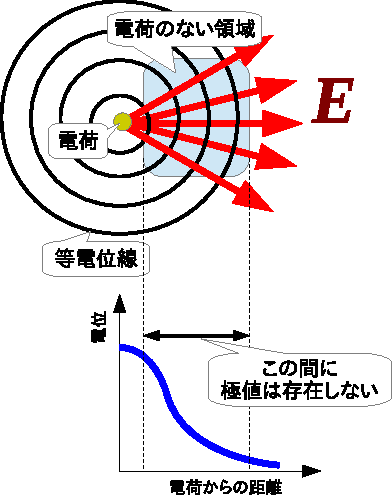
\includegraphics[keepaspectratio, width=6cm,height=7.74cm,clip]{StaticEF_Char1.pdf}
                        \caption{電荷が存在しない領域では,電位は極値をとらない}
                        \label{fig:StaticEF_Char1}
                    \end{center}
                \end{figure}

        \subsubsection{特徴2}\label{subsubsec:char2}
            等電位の閉曲面内に,電荷が存在しない場合,その内部領域全体の電位は,
            閉曲面の電位に等しく,一定である.これも,背理法で説明する.

            閉曲面の内部の電位が一定でない,と仮定する.
            閉曲面が等電位であることから,閉曲面上には電荷は存在しないので,
            この閉曲面の内側に,極値
                \footnote{
                    極値: 極大値あるは極小値のどちらかを指す総称.
                }
            が存在するはずである.
            極値が存在するということは,上記の特徴1の対偶から,
            閉曲面内に電荷が存在するはずである.
                \footnote{
                    特徴1の論理をかいつまむと,「極値が存在しない,ならば,電荷が存在しない」
                    となる.この対偶は,「電荷が存在する,ならば,極値が存在する」である.
                    一般に,「A$\Rightarrow$B」が成立するとき,その対偶「$\lnot$ B $\Rightarrow\lnot$ A」も
                    同時に成立する.
                }.
            しかし,これは,電荷が存在しないという前提に矛盾する.この矛盾は,
            閉曲面内の電位が一定でないという仮定からの帰結である.
            以上から,本特徴2を示せた.
                \begin{figure}[hbt]
                    \begin{center}
                        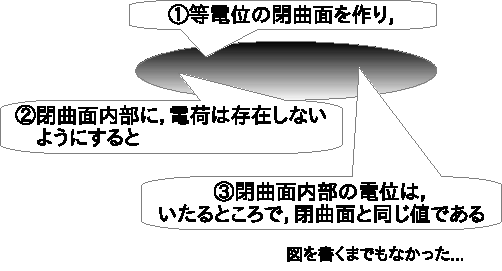
\includegraphics[keepaspectratio, width=6cm,height=5.4cm,clip]{StaticEF_Char2.pdf}
                        \caption{等電位の閉曲面内の電位(内部に電荷を含まず)}
                        \label{fig:StaticEF_Char2}
                    \end{center}
                \end{figure}


        \subsubsection{特徴3}\label{subsubsec:char3}
            任意の閉曲面において,閉曲面の内側の電荷分布と,閉曲面自体の電位が
            与えられれば,その領域内部の電位は,一意に決まる.

%       %==========================================================================
%       %  Subsection
%       %==========================================================================
        \subsection{アーンショーの定理}
        静電場中(ただし,電荷が存在しない領域に限る)では,荷電粒子は安定して存在できる
        位置がない.これを \textbf{アーンショーの定理} という
            \footnote{
                Samuel Earnshaw(1805--1888,イギリス):聖職者で数学者であった人らしい.
            }.
        この定理は,電場に限ったことではなく,磁場でも重力場でも成り立つ.
        距離に関する逆自乗の法則が成り立つならば,この定理が成立する.
                \begin{figure}[hbt]
                    \begin{center}
                        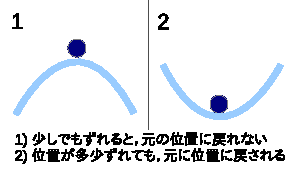
\includegraphics[keepaspectratio, width=5.11cm,height=2.91cm,clip]{Earnshow_000.pdf}
                        \caption{「安定な点」のイメージ}
                        \label{fig:Earnshow_000}
                    \end{center}
                \end{figure}

        実は,この定理は,すでに,上記の静電場の性質として,説明済みである.
        静電場に関するポアソン方程式からの帰結である.上記の性質をただ言い換えた
        だけだけど,この性質には「アーンショーの定理」とも呼ばれる別表現が
        あることを明記しておきたかった.


%   %==========================================================================
%   %  Section
%   %==========================================================================
    \section{導体}
        \begin{mycomment}
            導体といわれると,まず想像するのが,金属だろう.その他にも,
            炭素も有名だ.電解液(イオン溶液)も導体である
                \footnote{
                    ちなみに,純水は電気を通さない.水が電気を通すのは,
                    その中にイオンを含んでいる時のみであり,水道水が電気
                    を通すのも,それが完全な純水ではなく,不純物や塩素な
                    どのイオンを含んでいあるからである.
                }.
            なので,導体と言われても,想像される物質は色々と想像されてしまう.
            そこで,この章で考える導体の範囲に制限を与えることにしよう.
            ここで「導体」とよぶのは,金属や炭素などの個体で,その内部に
            自由電子をもつ物体を指すこととする.イオン溶液は確かに電気を
            通す導体ではあるが,除外する.
        \end{mycomment}

%   %==========================================================================
%   %  Subsection
%   %==========================================================================
    \subsection{導体とは}
        \subsubsection{導体,半導体,絶縁体}
        世の中には,様々な物体がある.石,木,水,葉,$\cdots$など,
        逐一例を上げていったのではきりがないほどだ.そして物体は,
        形,大きさ,硬さ,匂い,色,等,色々など性質をもっている.こういった性質の中で,
        電磁気学で特に興味がある性質に,"電気の通しやすさ" がある.
        電気の通しやすさは,物体を構成する物質そのものや,その構成に左右されるが,
        電磁気学ではそこまで細かいことは考えない
            \footnote{
                ここで学習する電磁気学は,現象論的なものである.
                物性などを含めて考えるときには,より詳細に,微視的
                な電磁気学を学習することも有用だが,内容が高度であるので,割愛する.
            }.
        目で見える範囲の物体を想像すれば十分である.
        とにかく,物体の塊を持ってきて,電気を通すか否かを判別するだけだ.
        物体の種類によって,電気の通しやすさは異なる.極端な例を上げると,
        ゴムは電気を通さないが,金属は電気を通す.様々な物体に対して,
        電気の通しやすさを調べると,それを順に並べることができる
            \footnote{
                電気の通しやすさを測定するには,対象となる物体の大きさを揃えたり,
                周囲の実験環境を揃えたりと,条件を一致させないといけない.
                ここでは,理想的に測ったと仮定しておこう.
            }.
        そうしてできた物体の順列で,電気を通しやすい部分に位置する物体のことを,
        \textbf{導体} という.反対に,電気を通しにくい部分に位置する物体のことは,
        \textbf{不導体} あるいは \textbf{絶縁体} という.
        簡単に言えば,導体とは電気を通しやすい物体のことである.
        また絶縁体は,電気を通しにくい物体のことを指す.

        ここで,"電気を通しやすい?" と表現した理由を説明しておこう
            \footnote{
                こんな回りくどい言い方をしないで,"電気を通す?" と表現したほうが,
                簡潔であると思われるかもしれないので.
            }.
        世の中には,様々な物体が存在するが,不思議な事に,「電気を(完全に)通さない
        物体」は存在しないのである.全ての物体が,電気を通すのである.ゴムなどの
        一般に電気を通さないとされる物体でも,詳細に測定すると,電気が流れることを
        確認できる.ただ,その流れる電気の量が非常に小さいので,電気を通していないと
        みなされるだけなのである.だから,電気を「通す/通さない」ではなく,
        「通しにくい/通しやすい」と書くべきなのである.

        とはいうものの,導体と絶縁体を明確に区別するような基準は存在しない.
        というか,定義すること困難なのである.導体と絶縁体とは,お互いに相対的な
        関係であり,状況によって変わりうるのである.例えば,紙は通常では絶縁体と
        して扱われるが,高電圧を紙にかける場合,電気を通すので,紙は導体として扱
        わないとならない.人間も,乾電池程度の電圧に対しては絶縁体だが,
        家庭用コンセントほどの電圧(100[V])に対しては導体となる
            \footnote{
                電化製品には,感電の恐れがあるという警告が大きく表示されているはず.
                特に,洗濯機において,アース(電気を体に通さないようにする仕組み)は絶対に
                欠かせない.
            }.
        では,導体と絶縁体の区別が全くできない程に曖昧かと
        言われれば,そうではない.\textbf{抵抗} という概念を使えば
            \footnote{
                オームの法則でお馴染みの,抵抗である.
            },
        ある程度区切りを入れることができる.抵抗による区切りも明確ではないが,抵抗は
        電気の通しやすさの1つの指標となる.
        抵抗は,電気物性を考えるときに重要な役割を果たす概念だが,電磁気学の
        理論的枠組を考える場合には,必要ではない
            \footnote{
                しかし,大切なので,後ほど解説をすることになるのだが$\cdots$.
            }.
        さしあたり,導体の例として金属をイメージすれば,十分である.また,
        絶縁体の例は,紙でも石でもゴムでもなんでもいい.
                \begin{figure}[hbt]
                    \begin{center}
                        \includegraphicslarge{DoutaiZetsuentai001.pdf}
                        \caption{導体と絶縁体}
                        \label{fig:DoutaiZetsuentai001}
                    \end{center}
                \end{figure}

        \subsubsection{理想的な導体}
            上記は,現実に存在する導体をイメージして記述した.
            これは,「物性物理学」よりの現実的な導体の説明である.
            しかし,多くの電磁気学の教科書で説明される「導体」は,
            少々異なる.
            電磁気学では,理論を考えやすくするために,理想化された導体を
            用いる.特に浸透している呼び方は無いようなので,
            このノートでは,\textbf{理想的な導体} と表現する.
            理想的な導体が,現実の導体と違う点を,いくつか上げておこう
                \footnote{
                    全部を上げることはできない.というか,思いつく限り上げたところで,
                    それで十分かどうかを判断することができないから.いや,
                    「理想的な導体」を理論的に整合性を保つように定義してやれば,
                    可能なのだけど,興味がない
                    (そんなことに時間をかけたくない,ってのが本音).
                }.
            \begin{myshadebox}{理想的な導体の性質}
                理想的な導体が持つ性質は,次の通り.
                \begin{enumerate}
                    \item 電荷には大きさがない(これは電磁気学全体をとおして同じ)
                    \item 正電荷と負電荷は導体中を自由に移動できる
                    \item 無限に多くの電荷をもっている(電荷の数に上限を与えない)
                    \item 導体中の電荷は,導体の外に出ることはできない
                    \item 連続分布している(原子レベルの不連続状態は考えない)
                \end{enumerate}
            \end{myshadebox}

            考えればいくらでも出てきそうだ
                \footnote{
                    教科書には,大抵の場合,こういった
                    ことは暗黙の了解として,明記されていない.紙面がもったいないからだろうか.
                    まあ,こんな約束なら,読めば簡単に悟れるから書くまでもないか.
                    書き始めるとキリがないし.
                }.
            この辺りで列挙を止めておこう.あとは,気が向いたら追記することにして,
            話をすめよう.

            上記の箇条書きに対して,補足しておきたい.理想的な導体を考える場合,
            それは原子で構成されていると考えてはいけない.確かに,正電荷と負電荷
            を持っているが,正電荷も導体内を自由に移動できるからだ.現実には,
            導体は原子で構成されていて,正電荷は動けない.正電荷も導体内を自由に移動
            できるという点が,はじめは違和感を感じるかもしれない.
                \begin{figure}[hbt]
                    \begin{center}
                        \includegraphicsdefault{risouteki_na_doutai000.pdf}
                        \caption{理想的な導体のイメージ}
                        \label{fig:DoutaiZetsuentai001}
                    \end{center}
                \end{figure}


%   %==========================================================================
%   %  Subsection
%   %==========================================================================
    \subsection{導体と電場の関係}
        \subsubsection{静電誘導}
        電場には,面白い性質がある.導体で囲まれた空間内部には電場は存在不可能
        なのである.導体はその内部に自由電子を含んでいる.この自由電子が,
        導体の外側の電場を打ち消すのである.
        自由電子は,導体中で移動できるため,導体の外側の電場から,
        クーロン力を受ける.自由電子は導体中に多数存在し,
        クーロン力に釣り合うように分布し,静止する.
        こうして静止した自由電子は,導体の外側の電場を完全に打ち消すように
        分布する.

        導体内部の自由電子が,外側の電場によって園分布が変わる現象を,
        \textbf{静電誘導} という.電子が電場に誘導されるイメージ.

        さらに言うと,電場は導体の表面で吸収され,導体中には浸透しない.
        導体内部が空洞だろうとなかろうと,導体の内部では一切電場は発生しない.
                \begin{figure}[hbt]
                    \begin{center}
                        \includegraphicsdefault{Doutai_to_Denba001.pdf}
                        \caption{静電誘導}
                        \label{fig:Doutai_to_Denba001}
                    \end{center}
                \end{figure}


        もちろん,電場を与えた
            \footnote{
                あるいは,電場の状態を変更しても同じこと.
            }
        直後は電荷の移動が起こるため,この間,導体内部にも電場が生じている.
        電荷がどのようにして導体中を移動するかも,興味のあるところだけど,
        ここでは,静電場内の現象を考えたいので,電荷の移動のことは後回し
        にしておこう.ここで考えたいことは,電荷の移動が完了したの,
        導体周辺に生じる静電場である.

        \subsubsection{静電遮蔽}
        上記の静電誘導の見方を変えると,
        導体の内部まで電場が突き抜けることはない,と言っても同じことだ.
        こうした立場からは,この現象を \textbf{静電遮蔽} という
            \footnote{
                あるいは,\textbf{静電シールド} とよばれれることもある.
            }.
        導体が電場を遮蔽するのだ.
                \begin{figure}[hbt]
                    \begin{center}
                        \includegraphics[keepaspectratio, width=6cm,height=4.2cm,clip]{Doutai_to_Denba000.pdf}
                        \caption{静電遮蔽}
                        \label{fig:Doutai_to_Denba000}
                    \end{center}
                \end{figure}

        電場の影響を極力少なくした実験を行う場合,この静電遮蔽が有効である.
        導体に完全に囲まれていれば,その中には電場は侵入してこないのだ.

        \begin{memo}{導体内部に電場は生じない}
            背理法を使って説明しよう(エネルギー保存則との矛盾をつかう).
            もし導体中に電場が発生すると仮定する.
            この時,導体内部の自由電子が,静電誘導を受け移動が始まる.
            しかし,これはエネルギー保存則に反する.なぜなら,
            エネルギーを与えていないにもかかわらず(電場はエネルギーではない),
            電流が生じるはずがないからだ.

            というか,そもそも,導体である条件の1つに,数え切らないくらいの
            自由電子をもっているという性質が要請されていて,電子は電場を吸収する
            のであるから,導体内部に電場が発生しないことは,導体の定義から直接的に
            示されるとも考えられる.
        \end{memo}

        \subsubsection{電場と導体表面}
        電場が導体の表面で吸収される場合,電場は導体表面に直交する.
        導体の形状がどんなに複雑でも,電場は表面に直角に交わる.
                \begin{figure}[hbt]
                    \begin{center}
                        \includegraphicsdefault{Doutai_to_Denba002.pdf}
                        \caption{電場は導体表面に直交する}
                        \label{fig:Doutai_to_Denba002}
                    \end{center}
                \end{figure}

        斜めに交わることはない.もし,斜めに交わってしまうと,導体表面に平行な電場成分が発生する.
        しかし,これは,先に示した導体の性質「導体内部に電場は生じない」と反する.だから,
        道内の内部に電場が生じないように交わるには,直角に交わるしかないのだ.
                \begin{figure}[hbt]
                    \begin{center}
                        \includegraphics[keepaspectratio, width=6cm,height=2.7cm,clip]{Doutai_to_Denba003.pdf}
                        \caption{もし,電場が導体に直交しなかったら...}
                        \label{fig:Doutai_to_Denba003}
                    \end{center}
                \end{figure}

%   %==========================================================================
%   %  Subsection
%   %==========================================================================
    \subsection{導体と電位の関係}
    導体の表面は等電位面である.導体がどんな形をしていても,等電位面になる.
    電場が導体に垂直に交わることから,簡単に説明できる.
    \ref{subsec:toudeni_denba}節を参照.




%===================================================================================================
%  Chapter : 磁束密度に対するガウスの法則
%  説明    : 磁束密度に対するガウスの法則ビオ・サヴァールの法則から導く
%===================================================================================================
\chapter{磁束密度に対するガウスの法則}
%   %-----------------------------------------------------------------------------------------------
%   %  Input
%   %    File Name : PhysNote_EM_1st_GaussLowBF.tex
%   %-----------------------------------------------------------------------------------------------
        %   %==========================================================================
%   %  Section
%   %==========================================================================
    \section{ビオ$=$サバールの法則(復習)}
        \begin{mycomment}
            ビオ$=$サバールの法則についての詳細は,\ref{subsec:BiotSavart_Gene}節を参照.
            以下は,そこからの抜粋である.
        \end{mycomment}

        ビオ$=$サバールの法則は,磁束密度に関する法則である.
        \begin{myshadebox}{ビオ$=$サバールの法則(電流密度表示)}
            電流はその周囲に磁束密度を発生させる.その発生は以下の式に従う.
            \begin{align}
                \bB(\br)
                = \frac{\mu_{0}}{4\pi}
                    \int \frac{ \bi(\br')\times (\br-\br') }{ |\br-\br'|^{3} } \df V'.
            \end{align}
        \end{myshadebox}
        \begin{figure}[hbt]
            \begin{center}
                \includegraphics[keepaspectratio, width=7.2cm, height=5.79cm, clip]{biot_savart_1.pdf}
                \caption{ビオ$=$サバールの法則}
            \end{center}
        \end{figure}


%   %==========================================================================
%   %  Section
%   %==========================================================================
    \section{磁束密度に対するガウスの法則の導出}
%   %==========================================================================
%   %  Subsection
%   %==========================================================================
    \subsection{公式の確認}
        ビオ$=$サバールの法則から,磁束密度に対するガウスの法則を導出する
        手順を示す.まず,導出の際に以下のベクトル解析の公式を使用する.
            \begin{align}\label{eq:kousiki_kakunin}
                \dgrad \left( \frac{1}{r} \right) = - \frac{\br}{r^{3}}.  \\
                \drot (a\bX) = (\dgrad a) \times \bX + a(\drot \bX).
            \end{align}
        ただし,$r=\sqrt{x^{2}+y^{2}+z^{2}}$ である.また,$a$ は任意の
        スカラー関数であり,$\bX$ はベクトル関数である.

        \begin{memo}{公式の変形1}
            この公式を使うのだけど,このまま適用するわけではない.
            適用しやすいように,形を変えておこう.上段の式から見ていこう.
                \begin{equation*}
                    \dgrad \left( \frac{1}{r} \right) = - \frac{\br}{r^{3}}.
                \end{equation*}
            の $\br$ に注目する.任意の定ベクトル $\bC$ を考えて,$\br$ を
                \begin{equation*}
                    \br \rightarrow \br - \bC
                \end{equation*}
            と置き換えてやる.すると
                \begin{equation*}
                    \dgrad \left( \frac{1}{|\br - \bC|} \right)
                    =
                    - \frac{\br - \bC}{{|\br - \bC|}^{2}}
                \end{equation*}
            となる
        \footnote{
                    計算は合成微分を繰り返し.面倒だが,$x$ 成分の
                    計算だけでよいので,手で計算してほしい.
                    ここでは,記述が面倒なので,結果のみとする.
                }.
        \end{memo}

        \begin{memo}{公式の変形2}
            任意の定ベクトル $\bX$ に対して,
                \begin{equation*}
                    \drot \bX = \b0
                \end{equation*}
            が成立するとき,
                \begin{equation*}
                    \drot (a\bX) = (\dgrad a) \times \bX
                \end{equation*}
            が成り立つ.
        \end{memo}

%   %==========================================================================
%   %  Subsection
%   %==========================================================================
    \subsection{導出}
        ベクトル解析の公式 $\ddiv (\drot \bX) = 0$ を念頭に置き,
        ビオ$=$サバールの法則の式を変形していこう.

        まず,ビオ$=$サバールの式を書き下す.
            \begin{align}
                \bB(\br)
                =\frac{\mu_{0}}{4\pi}
                \int\frac{\bi(\br')\times
                (\br-\br')
                }{|\br-\br'|^{3}}\df V'.
            \end{align}
        この式の
            \begin{equation*}
                \frac{\br-\br'}{|\br-\br'|^{3}}
            \end{equation*}
        の部分の注目すると,公式
            \begin{equation*}
                \dgrad \left( \frac{1}{|\br - \bC|} \right)
                =
                - \frac{\br - \bC}{{|\br - \bC|}^{2}}
            \end{equation*}
        から
            \begin{align}
                \bB(\br)
                =\frac{\mu_{0}}{4\pi}
                    \int
                        \bi(\br')\times
                            \biggl\{
                                - \dgrad \left( \frac{1}{|\br - \br'} \right)
                            \biggr\}
                    \df V'.
            \end{align}
        さらに,公式($\bU$ は定ベクトル,$a$ はスカラー関数)
            \begin{align*}
                \drot (a\bU) &= (\dgrad a) \times \bU  \\
                             &= -\bU \times (\dgrad a)  \\
                             &= \bU \times (- \dgrad a)
            \end{align*}
        により,
            \begin{align*}
                \bB(\br)
                &=\frac{\mu_{0}}{4\pi}
                    \int
                        \bi(\br')\times
                            \biggl\{
                                - \dgrad \left( \frac{1}{|\br - \br'|} \right)
                            \biggr\}
                    \df V'
                 \\
                &= \int
                        \drot \left( \bi(\br') \frac{1}{|\br - \br'|} \right)
                    \df V'
                 \\
                &= \int
                        \drot \left(\frac{ \bi(\br') }{|\br - \br'|} \right)
                    \df V'.
            \end{align*}
        積分と微分の順番を変更して,
            \begin{align}
                \bB = \drot \int \left(\frac{ \bi(\br') }{|\br - \br'|} \right) \df V'.
            \end{align}

        ここで,次のようなベクトル関数を定義する.
            \begin{align}
                \bA(\br) := \int \frac{ \bi(\br') }{|\br - \br'|} \df V'.
            \end{align}
        これは後で \textbf{ベクトル$\cdot$ポテンシャル} と呼ばれる量と同じものである
            \footnote{
                ここでは,あくまでも形式的に導入するものであり,その正式な導入は後で行う.
            }.
        この $\bA(\br)$ をにより,ビオ$=$サバールの法則は以下のような形になる.
            \begin{align}
                \bB(\br) = \drot \bA(\br).
            \end{align}

        ここまで計算すれば,明らかだ.両辺に $\ddiv$ をとろう.
            \begin{align}
                \ddiv \bB(\br) &= \ddiv \left( \drot \bA(\br) \right). \notag \\
                \therefore \quad
                \ddiv \bB(\br) = 0.
            \end{align}
        この計算で,公式 $\ddiv (\drot \bX) = 0$ を使った.
        これは,磁束密度に対するガウスの法則に他ならない.

        以上の計算から,ビオ$=$サバールの法則に従って生じる磁束密度は,
        ガウスの法則 $\ddiv \bB(\br) = 0$ を満たすことが示された.


%   %==========================================================================
%   %  Subsection
%   %==========================================================================
    \subsection{まとめ}
        以上の結果をまとめよう.
                    \begin{myshadebox}{静磁束密度のガウスの法則(微分形)}
                        時間変化のない磁束密度に対する,局所的な
                        ガウスの法則は,以下の微分形の式により表される.
                        \begin{align}
                            \ddiv \bB =0.
                        \end{align}
                    \end{myshadebox}
                    \begin{myshadebox}{静磁束密度のガウスの法則(積分形)}
                        時間変化のない磁束密度に対する,大局的な
                        ガウスの法則は,以下の積分形の式により表される.
                        \begin{align}
                            \int_{S} \bB(\br) \cdot \bn(\br)\df S=0.
                        \end{align}
                    \end{myshadebox}

            磁束密度に対するガウスの法則は,
            電場に対するガウスの法則
            と同様に考えられる.
            磁束密度に対するガウスの法則
            を表す式を見てみると,
            『任意にとった閉曲面からの磁束密度の
            流出量を積分すると,その値は 0 に
            なる』
            ということ解釈できる.後で確認することではあるが,微分形のマクスウェル方程式によれば,
            磁束密度は,どの場所においても,発生 や 吸い込み がおきていないことがわかる.
            それゆえに,磁束密度の流出も生じないのである.


%   %==========================================================================
%   %  Section
%   %==========================================================================
    \section{法則の意味(図的イメージ)}


%===================================================================================================
%  Chapter : アンペール$=$マクスウェルの法則
%  説明    :
%           1.ビオ$=$サバールの法則から,定常電流のアンペールの法則を導く
%           2.電荷保存則とアンペールの法則の矛盾をのぞくべく,「変位電流」を導入する
%           3.変位電流をアンペールの法則に組み込み,アンペール$=$マクスウェルの法則を導く
%===================================================================================================
\chapter{アンペール$=$マクスウェルの法則}
%   %-----------------------------------------------------------------------------------------------
%   %  Input
%   %    File Name : PhysNote_EM_1st_AMLaw.tex
%   %-----------------------------------------------------------------------------------------------
        %   %==========================================================================
%   %  Section
%   %==========================================================================
    \section{アンペールの法則}
%   %==========================================================================
%   %  Subsection
%   %==========================================================================
    \subsection{エルステッドの実験}
        電流が生じている導体のそばに方位磁針をおくと,方位磁針は南北を示さなくなる.
        エルステッド
            \footnote{
                Hans Christian \O rsted ( 1777 - 1851, デンマーク  ):物理学者,科学者.
                太田光一の著した「電磁気学の基礎\I」には,"エールステズ" と片仮名表記されている.
            }
        はこの現象を発見した.その後,更に多くの実験が行われた.そして,アンペールによって,
        \textbf{アンペール力} (2つの電流の間に生じる力) が発見された.アンペール力 $\bF$ は,
        2つの電流を $I$, $I'$ とし,その間の距離を $l$ としたとき,
            \begin{align}
                \bF = k\frac{II'}{l}
            \end{align}
        で表される.$k$ は比例定数である.$k$ の具体的な数値は後で考えることになる
            \footnote{
                SI単位系において,電流の基本単位1[A] はアンペール力と利用し,定義される.
            }.
        2つの電流の間に,引力もしくは斥力(反発力)が発生するということである.
        2つの電流が同じ方向に向いていれば引力が働く.逆向きであれば,斥力が働く.

        原理を考えてみよう.
        電流の周りには磁束密度が生じる.また,電流とは電荷のいどうのことである.
        一方の電流が作る磁束密度の中を,他方の電流のもとである電荷が移動することになる.
        となれば,電荷は磁束密度中をある速度を持って移動することになるので,
        ローレンツ力を受けることになる.電荷というスケールで考えると,
        ローレンツ力を受けているのであるが,電流という大局的な視点で考えれば,
        アンペール力が働いているのである.アンペール力は原理的にはローレンツ力に
        起因するものと考えても良いが,時と場合によって,使い分けることが大事だ.
        例えば,実験や工学的な目的であればアンペール力を利用したほうが便利だし,
        現象を理論的に追求しようとした場合,ローレンツ力として考えたほうが
        一般性が高まることもあるだろう.

        話がそれたが,この節で言いたかったことは,電流の周囲には磁束密度が生じるという
        ことである.では,具体的には,どのような磁束密度が分布しているのだろうか.
        以下で考えていこう.


%   %==========================================================================
%   %  Subsection
%   %==========================================================================
    \subsection{ビオ$=$サバールの法則(復習)}
        \begin{mycomment}
            ビオ$=$サバールの法則についての詳細は,\ref{subsec:BiotSavart_Gene}節を参照.
            以下は,そこからの抜粋である.
        \end{mycomment}
            \begin{myshadebox}{ビオ$=$サバールの法則(電流密度表示)}
                電流はその周囲に磁束密度を発生させる.その発生は以下の
                式に従う.
                \begin{align}
                    \bB(\br)
                    =\frac{\mu_{0}}{4\pi}
                    \int\frac{\bi(\br')\times
                    (\br-\br')
                    }{|\br-\br'|^{3}}\df V'
                \end{align}
            \end{myshadebox}
            \begin{figure}[hbt]
                \begin{center}
                    \includegraphics[keepaspectratio, width=7.2cm, height=5.79cm, clip]{biot_savart_1.pdf}
                    \caption{ビオ$=$サバールの法則}
                \end{center}
            \end{figure}

%   %==========================================================================
%   %  Subsection
%   %==========================================================================
    \subsection{アンペールの法則の導出}
%       %======================================================================
%       %  Subsection
%       %======================================================================
        \subsubsection{定常電流}
            ビオ$=$サバールの法則からアンペールの法則を
            導く.はじめに注意しておくと,ビオ$=$サバールの法則は時間変化しない電流
            についての法則である.このような電流を \textbf{定常電流} という.
            従って,以下に導くアンペールの法則も,定常電流を仮定していることになる.
          まず,定常電流を数式で表現しておく.

            電流とは電荷の集団の移動と定義される.電流が時間変化しないということは,
            電荷の移動の時間変化が一定であると考えられる.つまり,電荷密度の
            時間変化はないと解釈できる.ここで,
            電荷保存の法則をおもいだすと,
            \begin{align}
            \frac{\df }{\df t}\int_{\Omega_{S}} \rho(\br,t)\df V
            +\int_{S} \bi(\br,t)\cdot\textit{\textbf{n}}(\br)\df S=0
            \end{align}
            である.電荷密度 $\rho(\br,t)$ が一定の値をとることから,
            この式の第1項は 0 なる.つまり,この式に
            $\frac{\df }{\df t}\int_{\Omega_{S}} \rho(\br,t)\df V=0$ を
            代入して,
            \begin{align}
            \int_{S} \bi(\br,t)\cdot\textit{\textbf{n}}(\br)\df S=0
            \end{align}
            である.この式が定常電流を表現する式である.

%       %======================================================================
%       %  Subsection
%       %======================================================================
        \subsubsection{導出}
            定常電流であることを踏まえてアンペールの法則を導出する.ビオ$=$サバールの法則は
            式(\ref{Bior=savart'slow1})によって,
            \begin{align}
            \bB(\br)
            =\frac{\mu_{0}I}{4\pi}
             \int_{\Gamma}\frac{\bt(\br')\times
             (\br-\br')
            }{|\br-\br'|^{3}}\df s'
            \end{align}
            である.$\bt(\br')\df s'$ とまとめて,
            \begin{align}
            \bB(\br)
            =\frac{\mu_{0}I}{4\pi}
             \int_{\Gamma}\frac{\bt(\br')\df s'\times
             (\br-\br')
            }{|\br-\br'|^{3}}
            \end{align}
            である.
            この式の両辺を曲線 $\Gamma$ を内側に含む閉曲線 $l$ で線積分すると,
            \begin{align}
            &\oint_{l}\bB(\br)\cdot \bt(\br) \df l \notag \\
            &=\frac{\mu_{0}I}{4\pi}\oint_{l}
             \int_{\Gamma}\frac{\bt(\br')\df s'\times
             (\br-\br')
            }{|\br-\br'|^{3}}\cdot \bt^{\ast}(\br)
            \df l
            \end{align}
            とする.ここに,$\bt^{\ast}(\br)\df l$ は 閉曲線 $l$  単位
            接線ベクトル である.この式の右辺に ベクトル解析の公式
            \begin{align*}
            (\bL\times\bM)\cdot\bN
            =(\bN\times\bL)\cdot\bM
            \end{align*}
            を用いると,
            \begin{align}
            &\oint_{l}\bB(\br)\cdot \bt^{\ast}(\br) \df l \notag \\
            &=\frac{\mu_{0}I}{4\pi}\oint_{l}
             \int_{\Gamma}\frac{\bt^{\ast}(\br)\df l\times\bt(\br')\df s'
            }{|\br-\br'|^{3}}\cdot
            (\br-\br')
            \end{align}
            と変形できる.ここで,曲線 $\Gamma$ の単位接線方向ベクトル $\bt(\br')$ と
            閉曲線 $l$ の単位接線成分 $\bt^{\ast}(\br)$ との
            外積 $\bt(\br')\times\bt^{\ast}(\br)$ を
            \begin{align*}
            \textit{\textbf{n}}(\br')=\bt(\br')\times\bt^{\ast}(\br)
            \end{align*}
            とおく.また,$\df S_{l}=\df l\df s'$(「閉曲線 $l$ を縁とする面」という意味)とおく.すると,
            \begin{align}
            \oint_{l}\bB(\br)\cdot \bt^{\ast}(\br)\df l
            =\frac{\mu_{0}I}{4\pi}\oint_{l}
             \int_{S_{l}}\frac{\textit{\textbf{n}}(\br')\df S
            }{|\br-\br'|^{3}}\cdot
            (\br-\br')
            \end{align}
            と書ける.
            さらに曲線 $\Gamma$ が,閉曲線 $l$ の内側にあるので,公式
            \begin{align*}
            &\int_{S_{l}}\frac{\textit{\textbf{n}}(\br')\df S
            }{|\br-\br'|^{3}}\cdot
            (\br-\br') \\
            &=\int_{S_{l}}\frac{\textit{\textbf{n}}(\br')
            }{|\br-\br'|^{3}}\cdot
            (\br-\br')\df S=4\pi
            \end{align*}
            が成り立つ.従って,
            \begin{align}
            \oint_{l}\bB(\br)\cdot \bt^{\ast}(\br)\df l
            =\mu_{0}I
            \end{align}
            となる.この計算では,閉曲線 $l$ の単位接線ベクトルとして,$\bt^{\ast}(\br)$ を
            用いてきたが,ここで改めて,$\bt(\br)=\bt^{\ast}(\br)$ と
            書くことにしても混乱はないので,
            \begin{align}
            \oint_{l}\bB(\br)\cdot \bt(\br)\df l
            =\mu_{0}I
            \end{align}
            さらに,面 $S_{l}$ を流れる電流 を電流密度で表記すると,
            \begin{align}
            I=\int_{S_{l}} \bi(\br)\cdot\textit{\textbf{n}}(\br)\df S_{l}
            \end{align}
            と書けることから
            \footnote{
            この式の $S_{l}$ は閉曲面ではない.$S_{l}$ は
            閉曲線 $l$ を縁とした曲面である. → 電荷保存の法則で考えているのは
            閉曲面 $S$ であって,これとの違いに注意をする.
            },(電流は定常電流である.)
            \begin{align}
            \oint_{l}\bB(\br)\cdot \bt(\br)\df l
            =\mu_{0}\int_{S_{l}} \bi(\br)\cdot\textit{\textbf{n}}(\br)\df S_{l}
            \end{align}
            と表現できる.何度も確認するが,この式の $\bt(\br)$ は
            閉曲線 $l$ の単位接線ベクトルである.
                \begin{myshadebox}{アンペールの法則(積分形)}
                    電流の周囲には磁束密度が生じ,以下の式に従う.
                    \begin{align}
                        \oint_{l} \bB(\br)\cdot\bt(\br)\df l
                        =\mu_{0}\int_{S_{l}} \bi(\br)
                        \cdot\textit{\textbf{n}}(\br)\df S_{l}
                    \end{align}
                \end{myshadebox}

%   %==========================================================================
%   %  Subsection
%   %==========================================================================
    \subsection{法則の意味(図的イメージ)}
        言葉で言えば,「磁束密度 $\bB(\br)$ が
        存在する場所において,任意の閉曲線 $l$ を描き,この閉曲線 $l$ の接線方向に線積分すると,
        その値は閉曲線 $l$ の張る面 $S_{l}$ を貫く電流 $I$ の $\mu_{0}$ 倍に等しい」と言える.
        この式の解釈を簡単にいえば,『電流が磁束密度を生じさせる』ということである.
        つまり,(定常的な)磁束密度が存在するならば,その根源は電流である と言える.

        アンペールの法則を満たす磁束密度は一意に定まらない.そこで,静電場で考えた時と同じように
        磁束密度に対するガウスの法則を導入するのである.このガウスの法則によって,
        磁束密度を一意に決定できるようになる.

%   %==========================================================================
%   %  Section
%   %==========================================================================
    \section{アンペール$=$マクスウェルの法則}
    \begin{mycomment}
        アンペール$=$マクスウェルの法則とは,その記述から察しがつくと
        思うが,アンペールの法則にマクスウェルが改良を加えたものである.
        マクスウェルは,動電磁場を考える場合に,アンペールの法則が不完全
        であるとし,\textbf{変位電流} という新しい概念を導入した.変位電流とは
        なんなのか.マクスウェルはどのように修正したのか.その拡張された
        法則はどういったイメージなのか.この節で考えることにしよう.
    \end{mycomment}

%   %==========================================================================
%   %  Subsection
%   %==========================================================================
    \subsection{アンペールの法則と電荷保存則との矛盾}
        マクスウェルは,アンペールの法則に変位電流の項を加える修正を行った.
        なぜ,このような修正が行われたかというと,アンペールの法則が電荷保存則を
        満たさなかったからである.アンペールの法則は,電荷保存則と矛盾するのだ.
        この矛盾はどういったものなのかを,以下に示す.
            \begin{equation*}
                \drot \bB = \mu_{0}\bi.
            \end{equation*}
        両辺に発散($\ddiv$;divergence)をとってみる.
            \begin{equation*}
                \ddiv( \drot \bB ) = \ddiv ( \mu_{0}\bi ).
            \end{equation*}
        ここで,ベクトル解析の公式から,$\ddiv( \drot \bB ) = 0$ が成立している
            \footnote{
                (公式;定理)任意のベクトル $\bX$ にたいして,
                    \begin{equation*}
                        \ddiv( \drot \bX ) = 0
                    \end{equation*}
                が成立する.
            }.
        つまり,
            \begin{align*}
                \ddiv ( \mu_{0}\bi ) &= 0  \\
                \therefore \quad
                \ddiv \bi &= 0 \,,
                \quad(\because \mu_{0}\mbox{は定数})
            \end{align*}
        となる.ここで,式の見やすさの為に,右辺と左辺を入れ替えた.
        アンペールの法則を認める限り,この式が成立していなければ
        ならないのだけど,一方で,電荷保存則は
            \begin{equation*}
                \ddiv \bi = -\frac{\rd \rho}{\rd t}.
            \end{equation*}
        であり,右辺に関して,$\rd \rho/\rd t \neq 0$ である.
        明らかに,アンペールの法則と電荷保存則は矛盾してしまう.
        どちらが間違っているのだろうか.あるいは,両者とも間違って
        いるのだろうか.マクスウェルの出した答えは,アンペールの法則
        が不完全であるというもので,\textbf{変位電流} という概念を持ち出して,
        修正を加えた.現在では,変位電流の実在性は,電磁波の実験により確固たる
        ものとなっている.

%   %==========================================================================
%   %  Subsection
%   %==========================================================================
    \subsection{変位電流}
        マクスウェルが導入した変位電流とはどのようなものであり,また,
        変位電流の導入はアンペールの法則と電荷保存則の矛盾をどのように解決するか.
        これらを次に確認しよう.
        それには,
        電場に対するガウスの法則に,電荷密度 $\rho$ が現れていることに着目し,
        ここから電荷保存則の式に似せていくという,アプローチをとる.

        電場に対するガウスの法則によれば,
            \begin{align*}
                \ddiv \bE = \frac{1}{\varepsilon_{0}}\rho.
            \end{align*}
        両辺を時間 $t$ で微分する.
            \begin{align*}
                  \frac{\rd}{\rd t}\left(\ddiv \bE \right)
                = \frac{\rd }{\rd t}\left(\frac{1}{\varepsilon_{0}}\rho\right).
            \end{align*}
        ここで,空間に関する微分 $\ddiv$ と時間に関する微分 $\rd/\rd t$ の
        可換性を仮定して
            \footnote{
                時間微分と空間微分は可換であると,信じられている.
                ちなみに,ここに言う「可換」とは,演算の順番のことを言っている.
                つまり,時間微分と空間微分の計算順序を入れ替えてもよい,ということを
                主張している.要は,「空間に関するな微分演算」と「時間」に関する微分演算
                は独立していて,どちらを先に実行しようが,計算結果は変わらないということ.
            },
            \begin{equation*}
                  \ddiv \left(\frac{\rd \bE}{\rd t} \right)
                = \frac{1}{\varepsilon_{0}}\frac{\rd \rho}{\rd t}
            \end{equation*}
        となる.両辺に,$\varepsilon_{0}$ を掛けると,
            \begin{equation*}
                  \ddiv \left(\varepsilon_{0}\frac{\rd \bE}{\rd t} \right)
                = \frac{\rd \rho}{\rd t}.
            \end{equation*}
        最後に,両辺に$-1$をかける.
            \begin{equation*}
                  \ddiv \left( - \varepsilon_{0}\frac{\rd \bE}{\rd t} \right)
                = - \frac{\rd \rho}{\rd t}.
            \end{equation*}
        ここで,再度,電荷保存則の式を見てみよう.
            \begin{equation*}
                \ddiv \bi = -\frac{\rd \rho}{\rd t}.
            \end{equation*}

        電荷保存則と見比べてみると,$- \varepsilon_{0}(\rd \bE/\rd t)$ が
        電流密度と同じ働きをすることが見て取れる.しかし,この項は電流密度そ
        のものを表しているのではない事に注意しよう.
        この項 $\varepsilon_{0}(\rd \bE/\rd t)$ は \textbf{変位電流} とよばれる.

        電場の時間変化 $- \varepsilon_{0}(\rd \bE/\rd t)$ が,電流のように振る舞うように見える.
        考察している範囲に電荷密度が存在していなくとも,電場の時間変化が生じていれば,それを
        電流とみなして良いことを示唆していそうだ.
        アンペールの法則と電荷保存則との矛盾を解く鍵だと言っていい.
        実際にマクスウェルはこの項を持ち出して,アンペールの法則に手を加えて,矛盾を解消した.

%   %==========================================================================
%   %  Subsection
%   %==========================================================================
    \subsection{アンペール$=$マクスウェルの法則の導出}
        アンペール$=$マクスウェルの法則とは,前にも書いた通り,
        アンペールの法則に変位電流の考えを加えたものである.
        その方程式を先に書いてみれば,
        \begin{align}
            \drot \bB
                =   \mu_{0} \bi
                  + \varepsilon_{0} \mu_{0} \frac{\rd \bE}{\rd t}.
        \end{align}
        この方程式は,アンペールにより発見された \textbf{アンペールの法則} に,
        マクスウェルが修正を加えたもので,\textbf{アンペール$=$マクスウェルの法則} と
        よばれる.

        式の形を見るとは,単に,アンペールの法則の右辺に,
        変位電流を加えただけだ.しかし,電荷保存則との矛盾が解消されている.
        右辺第二項の $\varepsilon_{0} \mu_{0} (\rd \bE/\rd t)$ が
        あるため,$\ddiv \bi=0$ となっても,
                \begin{equation*}
            \drot \bB = \varepsilon_{0} \mu_{0} \frac{\rd \bE}{\rd t}.
                \end{equation*}
        となって,電荷保存則と矛盾はしない.
        この式を解釈すると,電場の時間変化が回転する磁場を発生させる,
        ということになる.

%   %==========================================================================
%   %  Subsection
%   %==========================================================================
    \subsection{法則の意味(図的イメージ)}

%   %==========================================================================
%   %  Section
%   %==========================================================================
    \section{静電容量}
%   %==========================================================================
%   %  Subsection
%   %==========================================================================
    \subsection{キャパシタンス}

    \begin{memo}{「キャパシタ」と「キャパシタンス」の違い}
    \end{memo}

%   %==========================================================================
%   %  Subsection
%   %==========================================================================
    \subsection{変位電流とキャパシタ}

%   %==========================================================================
%   %  Subsection
%   %==========================================================================
    \subsection{平行平板型のキャパシタ}

%   %==========================================================================
%   %  Section
%   %==========================================================================
    \section{電流のSI単位に基づく定義}
%   %==========================================================================
%   %  Subsection
%   %==========================================================================
    \subsection{直線電流が作る磁束密度}
        さて,今まで電流の単位として [A]=[C・s] を用いてきたが,
        先にも書いたように,これは現実の定義とは違うものである.
        SI単位系における基本単位は,電荷ではなく,電流が
        採用されている.

        今までの議論で電流を定義するための準備
        ができたので,そのための準備としてのこの項目と,次も項目で,
        電流の定義をし直すことにする.

        まず,定義の概略を示しておく.電流は電荷の移動によって生じる現象であるので,
        電流はローレンツ力を受ける.この電流に対するローレンツ力を人間が観測する
        するときは,導線が受ける力として観測される.
        その力は $\bF=\textit{\textbf{I}}\times \bB$ で表現できた.
        ここで,2つの平行な直線の導線を用意する.この2つの導線に同じ向きに電流を流すと,後に示すように,
        導線が互いに引き合う現象が生じる
        \footnote{
            電流を逆向きに流せば,導線同士は互いに反発しあう.
        }
        .この力によって電流を定義するのである.実際の力の大きさとしては $2\times 10^{-7}$ [N/m] が
        採用されている.
        導線同士が互いに引き合うのはローレンツ力によるものであり,これは
        一方の電流の作る磁束密度が,他方の電流(電荷)に及ぼすローレンツ力である.
        従って,1つの導線に流れる電流が作る磁束密度を計算する必要があり,
        ここではその計算をすることが目的である.そして,次の項目でここでの計算結果を
        利用して,電流を定義していこうと考える.

        直線電流が図\ref{fig:den_jisoku}のような磁束密度を作ることを確認する.
        1本の直線な導線を用意する.この導線に定常電流 $\textit{\textit{i}}$ を流し,
        この定常電流がその周囲に作る磁束密度を考える.
        アンペールの法則は
                    \begin{align}
                        \oint_{l} \bB(\br)\cdot\bt(\br)\df l
                        =\mu_{0}\int_{S_{l}} \bi(\br)
                        \cdot\textit{\textbf{n}}(\br)\df S_{l}
                    \end{align}
        のように書かれる.
            \begin{figure}[hbt]
                \begin{tabular}{cc}
                    \begin{minipage}{0.5\hsize}
                \begin{center}
                    \includegraphicsdouble{den_jisoku.pdf}
                    \caption{電流の作る磁束密度}
                    \label{fig:den_jisoku}
                \end{center}
                    \end{minipage}
                    \begin{minipage}{0.5\hsize}
                \begin{center}
                    \includegraphicsdouble{den_lorentz.pdf}
                    \caption{電荷の磁束密度から受けるローレンツ力}
                    \label{fig:den_lorentz}
                \end{center}
                    \end{minipage}
                \end{tabular}
            \end{figure}

        磁束密度の大きさは,ビオ$=$サバールの法則から,
        導線から等距離にある部分では等しくならないといけない.
        従って,直線の導線の任意の点を流れる電流が起こす,磁束密度の
        大きさが等しい部分をつないでいけば,その形は閉じた
        円になる.そして磁束密度の向きは電流の生じる方向に対して
        右回りである.図\ref{fig:den_lorentz}参照.これがわかれば,
        アンペールの法則の左辺;$\oint_{l} \bB(\br)\cdot\bt(\br)\df l$ の
        積分経路は,円にとればよいことがわかる.

        積分経路を円とすれば,その半径を $r$ とした場合に,
        磁束密度の強さは,以下のように計算される.

        アンペールの法則の左辺を計算すると,
            \begin{align*}
                \mbox{(左辺)}=\oint_{l} \bB(\br)\cdot\bt(\br)\df l
                      =\oint_{l}B\,\df l=B\oint_{l}\,\df l
            \end{align*}
        ここで,積分経路 $l$ は円であるので,$\oint_{l}\,\df l=2\pi r$ である.従って,
            \begin{align*}
                \mbox{(左辺)}=2\pi rB
            \end{align*}
        右辺;$\mu_{0}\int_{S_{l}} \bi(\br)\cdot\textit{\textbf{n}}(\br)\df S_{l}$ は,
        定常電流であるので,これは $\mu_{0}I$ と書ける.

        以上から
            \begin{align*}
                2\pi rB=\mu_{0}I
            \end{align*}
        すなわち,
            \begin{align}
                B=\frac{\mu_{0}I}{2\pi r}
            \end{align}
        である.

        \begin{memo}{積分経路を円にとる}
            なぜなら,円でない曲線経路を
            とったとしても,磁束密度の向きは円方向を向いているからである.
            下図参照.
                \begin{figure}[hbt]
                    \begin{center}
                        \includegraphics[keepaspectratio, width=6cm,height=6cm,clip]{dentei1.pdf}
                        \caption{閉曲線の取り方}
                        \label{fig:dentei1}
                    \end{center}
                \end{figure}

            図で示したように,曲線の接線と磁束密度の内積をとるので,
            接線の磁束密度に直角な方向成分は考察する必要がないのである.
            (考えたとしても,内積は0となるので意味がない.)
        \end{memo}

%   %==========================================================================
%   %  Subsection
%   %==========================================================================
    \subsection{電流が受ける力}
            電気量 $q$,速度 $\bv$  をもつ1つの電荷が受けるローレンツ力 $\bF$ をおもいだすと,
            \begin{align}
            \bF=q\bv\times\bB
            \end{align}
            であった.
            複数の電荷を考えれば,電荷密度という概念を導入して,
            \begin{align}
            \bF=\left(\int_\Omega \rho(\br)\df V\right)
            \langle\dot{\br}\rangle\times\bB
            \end{align}
            ここに,$\langle\dot{\br}\rangle$ は電荷のドリフト速度である.
            ドリフト速度というのは,複数の電荷の移動速度の平均である.
            そして,$Q:=\int_\Omega \rho(\br)\df V$ おくと,
            $\bF=Q
            \langle\dot{\br}\rangle\times\bB$ と書けて,
            $Q\langle\dot{\br}\rangle$ は電流を表現していると考えられるから,
            これを $\textit{\textbf{I}}$ おくことで($\textit{\textbf{I}}:= Q\langle\dot{\br}\rangle$),
            \begin{align}
            \bF=\textit{\textbf{I}}\times\bB
            \end{align}
            を得る.

%   %==========================================================================
%   %  Subsection
%   %==========================================================================
    \subsection{電流の定義(1[A]の定義)}\label{denryuuteigi}
            電磁気学ではSI単位系において,電流の単位が基本単位として
            採用されている.ここではその基本単位となる電流の1[A]を
            定義する.一つ前の項目\ref{dennryuunoukerutikara}で
            電流が受ける力は,導線の受ける力として現れることを確認し,
            その力は式(\ref{denruu_F})で表された.それをもう一度
            書き下せば,
                \begin{align}
                    \bF=\textit{\textbf{I}}\times \bB
                \end{align}
            である.
            \begin{figure}[hbt]
                    \begin{center}
                        \includegraphicsdefault{denryu_teigi.pdf}
                        \caption{電流の定義の説明図1}
                        \label{fig:denryu_teigi}
                    \end{center}
                \end{figure}

            2本の平行に並んだ導線を用意する.導線の名前をそれぞれ1,2とする.
            この2本の導線に定常電流を流す.それら2つの定常電流を
            それぞれ $\textit{\textit{i}}_{A}$,$\textit{\textit{i}}_{B}$ と
            する.この内の一方の導線に流れる電流が作る磁束密度を考える.
            どちらでもよいが $\textit{\textit{i}}_{1}$ の作る磁束密度を考える.
            アンペールの法則より,
                \begin{align*}
                    \oint_{l} \bB(\br)\cdot\bt(\br)\df l
                    =\mu_{0}\int_{S_{l}} \bi_{1}(\br)
                    \cdot\textit{\textbf{n}}(\br)\df S_{l}
                \end{align*}
            これは前項目で計算計算したように,
                \begin{align*}
                    B=\frac{\mu_{0}I_{1}}{2\pi r}
                \end{align*}
            である.従って,他方の導線に与える力は,
            (電流と磁束密度のなす角は $\pi/2$ であることに注意して)
                \begin{align*}
                    F=I_{2}B\sin\frac{\pi}{2}=I_{2}B
                \end{align*}
            従って,$B=\mu_{0}I_{1}/2\pi r$ を代入すれば.
                \begin{align}
                F=\frac{\mu_{0}I_{1}I_{2}}{2\pi r}
                \end{align}
            である.
            この式を用いて1[A]の電流を定義する.図\ref{fig:AARA}に描いたように,
            重さ $2\times10^{-7}$[N] のおもりを,同線の片方につるす.
                \begin{figure}[hbt]
                    \begin{center}
                        \includegraphics[keepaspectratio, width=5cm,height=4.5cm,clip]{AARA.pdf}
                        \caption{電流の定義の説明図2}
                        \label{fig:AARA}
                    \end{center}
                \end{figure}

            このとき,各導線には同じ方向に電流が流れているとする.
            導線間の距離は1[m]としている.
            この状態で,釣り合いが取れたとき,1[A]の電流が流れていると
            定義するのである.

            以上のことを形式的にまとめておこう.
                \begin{myshadebox}{電流1[A]の定義}
                    1[m]の間隔をおいた
                    2本の平行導線に電流を流して,
                    この導線に働く力が単位長さ(1[m])当たり $2\times10^{-7}$[N] の
                    力が働くとき,
                    この時に流れる電流を1[A]
                    と定義する.
                \end{myshadebox}


%===================================================================================================
%  Chapter : ファラデーの電磁誘導の法則
%  説明    :
%           1.ビオ$=$サバールの法則から,定常電流のアンペールの法則を導く
%           2.電荷保存則とアンペールの法則の矛盾をのぞくべく,「変位電流」を導入する
%           3.変位電流をアンペールの法則に組み込み,アンペール$=$マクスウェルの法則を導く
%===================================================================================================
\chapter{ファラデーの電磁誘導の法則}
%   %-----------------------------------------------------------------------------------------------
%   %  Input
%   %    File Name : PhysNote_EM_1st_EInduction.tex
%   %-----------------------------------------------------------------------------------------------
        %   %==========================================================================
%   %  Section
%   %==========================================================================
    \section{ファラデーの実験}
%   %==========================================================================
%   %  Subsection
%   %==========================================================================
    \subsection{起電力}
        「起電力」とは電流を発生させるためのエネルギー源である.
        具体的には 電池 と考えてよい.とにかく,電流を発生させる
        ものである.実際は,電流は電荷の移動であるので,従って,
        「起電力」とは電荷を動かすものである.電荷を動かすものと
        いえば,電場である.すなわち,起電力とは電場を導体内に発
        生させるエネルギー源であると言える.エネルギーと仕事の関
        係から,起電力は「導体内において,単位電荷を周させる仕事
        」と考えられる.従って,起電力を $V_{l}$ と書くと,(回路
        として閉ループ $l$ を想定するために,このような添え字を
        つけた.)
            \begin{align}
                V_{l}=\oint_{l} \bE(\br,t)\cdot\bt(\br,t) \,\df l
            \end{align}
        なる関係式を得ることができる.以後,\textbf{起電力} とは
        この $V_{l}$ のこという.


%   %==========================================================================
%   %  Subsection
%   %==========================================================================
    \subsection{磁束}
        イメージを先に書くと,「磁束蜜度の束」である.
        これは以下のように表現される.磁束密度を
        閉ループ $l$ を縁とする面 $S_{l}$ で面積分して,
            \begin{align}
                \Phi_{l}=\int_{S_{l}} \bB(\br,t)
                \cdot\textit{\textbf{n}}(\br,t) \,\df S_{l}
            \end{align}
        である.この $\Phi_l{}$ を \textbf{磁束} という.
            \begin{figure}[hbt]
                \begin{center}
                    \includegraphicsdefault{jisoku_image.pdf}
                    \caption{磁束のイメージ}
                    \label{fig:jisoku_image}
                \end{center}
            \end{figure}

%   %==========================================================================
%   %  Subsection
%   %==========================================================================
    \subsection{電磁誘導の法則}
            前にもビオ$=$サバールの法則の部分で書いたが,エルステッドは電流が生じるとそ
            の周りには磁束密度ができることを発見した
                \footnote{
                    電流を流している導線の近くに,方位磁針をいくつか置いてみると,
                    方位磁針は電流の作る磁束密度の方向に振れる.
                }.
            この現象はビオ$=$サバールの法則によって数学的に表現され,さらに,
            アンペールの法則と磁束密度に対するガウスの法則に形を変えている.

            ファラデーは電流が磁束密度を作るのならば,その逆作用として,磁束密度の
            中に置いた回路に電流が生じるのではないかと考えた.その実験の中で,彼
            は磁束密度の時間変化が電場を発生させることを発見した.そして,ノイマン
                \footnote{
                    Frantz Ernst Neumann:(1798 - 1895, ドイツの物理学者,鉱物学者)
                }
            は,この電磁誘導の法則を次のように定式化した.\\
                \begin{center}
                    \begin{itembox}[l]{\textbf{ファラデーの電磁誘導の法則}}
                        閉曲線 $l$ が張る曲面 $S_{l}$ を貫く磁束 $\Phi_{l}$ が時間変化すると,
                        この閉路 $l$ に起電力 $V_{l}$ が生じる.
                        この起電力 $V_{l}$ の大きさは,磁束 $\Phi_{l}$ の
                        時間変化率$\rd \Phi_{l}/\rd t$ に比例する.
                        また,起電力 $V_{l}$ の向きは,
                        この起電力によって閉路 $l$ に電流が生じるときに,
                        この電流が作る磁束がはじめの
                        磁束の変化を打ち消すような向きである.
                        起電力の向きに関すること
                        は \textbf{レンツの法則} とよばれる.
                        磁束 $\Phi_{l}$ の時間変化による閉路 $l$ 内に
                        生じる起電力 $V_{l}$ を,\textbf{誘導起電力} という.
                        ファラデーの電磁誘導の法則は,次式によって表される.
                        \begin{align}\label{denjiyudo}
                        V_{l}=-\frac{\rd \Phi_{l}}{\rd t}
                        \end{align}
                        誘導起電力によって回路に電流が生じるときに,
                        この電流が作る磁束がはじめの磁束の変化のきを正の向きとした.
                    \end{itembox}
                \end{center}

%   %==========================================================================
%   %  Subsection
%   %==========================================================================
    \subsection{法則の意味(図的イメージ)}
                電磁誘導の最も直感的なイメージを図\ref{fig:denjiyuudou},\ref{fig:denjiyuudou3}に示す
                    \footnote{図\ref{fig:denjiyuudou3}は
                        \url{http://vanity-worth.com/nature-law/lenz-1.htm}より(2008.08.24現在).
                    }.
                磁石が振動することによって,その磁石から生じている磁束が
                時間変化することになる.従って,この磁束密度の時間変化により,
                電場が生じることになる.もし,振動している磁石の周りに回路があるならば,
                回路の導線内には電場が生じ,従って起電力となる.
            \begin{figure}[hbt]
                    \begin{center}
                        \includegraphicsdefault{dennjiyuudou.pdf}
                        \caption{電磁誘導1-1}
                        \label{fig:denjiyuudou}
                    \end{center}
            \end{figure}
            \begin{figure}[hbt]
                    \begin{center}
                        \includegraphicsdefault{dennjiyuudou3.pdf}
                        \caption{電磁誘導1-2}
                        \label{fig:denjiyuudou3}
                    \end{center}
            \end{figure}

            電磁誘導の法則を別のイメージで考えてみる.原理は同じだが,次の例は
            とても面白い現象が得られる.

            コイルに電流を流すと磁束密度が生じることは,アンペールの法則から説明される.
            そこで,互いに近くに置かれた
            コイルを2つ用意し,片方(コイル1)にスイッチと電源を接続して,もう一方(コイル2)には
            何も接続しないようにする.図\ref{fig:denjiyuudou2}参照.

            まず初めの状態として,コイル1が電源に接続されスイッチが切れいている状態にする.
            このときはコイル1に電流が流れて得ておらず,従って,コイル1には磁束密度は
            生じていない.この状態からスイッチを入れてコイル1に電流を流してみると,
            この電流によってコイル1に電流が生じる.この電流は磁束密度を発生させる.
            つまり,コイル1の周りに「磁束密度の変化」があったことになる.
            ファラデーの電磁誘導の法則は,磁束密度の変化が回転する電場を生じさせるという
            ものであったので,
            この磁束密度の変化がコイル2の部分においても生じているはずであり,
            従って,コイル2に回転する電場が生じるはずである.つまり,
            コイル2に電流が生じるのである(電源がつながれていないのにもかかわらず!!).
                \begin{figure}[hbt]
                    \begin{center}
                        \includegraphicsdefault{dennjiyuudou2.pdf}
                        \caption{電磁誘導2}
                        \label{fig:denjiyuudou2}
                    \end{center}
                \end{figure}

            電磁誘導の法則(\ref{denjiyudo})を 電場 と 磁束密度 を用いて
            表現すれば,起電力 と 磁束 の項目から,次のように表現できる.
                    \begin{myshadebox}\textbf{ファラデーの電磁誘導の法則}
                        \begin{align}
                        \oint_{l} \bE\cdot\bt \,\df l =-\frac{\rd}{\rd t}\int_{S_{l}} \bB \cdot\textit{\textbf{n}} \,\df S_{l}
                        \end{align}
                        ここに,$\bE:=\bE(\br,t)$,$\bt:=\bt(\br,t)$,$\bB:=\bB(\br,t)$,$\bn:=\textit{\textbf{n}}(\br,t)$ であり,
                        位置と時間の関数である.これらが時間依存している点が重要である.
                        時間依存していなければ右辺は定数となり,静電場の方程式となる
                            \footnote{
                                この意味で,ファラデーの電磁誘導の法則は,静電場の方程式の
                                時間依存的な拡張と見ることもできる.
                            }.
                    \end{myshadebox}

%   %==========================================================================
%   %  section
%   %==========================================================================
    \section{自己誘導 / 相互誘導}
%   %==========================================================================
%   %  Subsection
%   %==========================================================================
    \subsection{自己インダクタンス}
        アンペールの法則によると,磁束密度 $B$ は電流 $I$ に比例する.
        先に見たとおり,磁束 $\Phi$ は 磁束密度 $B$ に比例するので
            \footnote{
                そのように,磁束を定義したのであった.
            },
        当然,\textbf{磁束は電流に比例する}.
            \begin{equation*}
               \Phi \propto B \propto I.
            \end{equation*}
        従って,磁束 $\Phi$ と電流 $I$ の関係式は,
        比例定数を $L$ としたときに,
            \begin{equation*}
                \Phi = LI.
            \end{equation*}
        これを電磁誘導の法則 $V=-\df \Phi/\df t$ に代入すると,
            \begin{align}
                V=-\frac{\df \Phi}{\df t}
                 =-L\frac{\df I}{\df t}
            \end{align}
        となる.この定数 $L$ を \textbf{自己インダクタンス} とよぶ.

        物理的イメージを考えてみよう.アンペールの法則により,電流は
        その周囲に磁束密度を発生させる.一方で,電磁誘導の法則によれば,
        時間変化する磁束密度の周囲には,電場が生じ,電位差が発生する.
        とすると,電流が流れていなかった導線に,突然に電流が流れ始めると,
        その周囲に磁束密度が発生するのだが,この磁束密度は時間変化するものであるので,
        同時に電位差もその周囲に生まれることになる.当然,いま流れ始めた電流は
        この電位差の影響もうけることになる.電流自身がその周囲に電位差を作り出し,
        その電位差が自身に帰ってくるのである."自己"インダクタンスと表現されている
        のは,この現象に由来している.

        \begin{memo}{磁束は電流に比例する}
            以下のように,簡略表記すると,わかりやすい.
            一重巻きのコイルを想定してみればよい.
            積分形のアンペールの法則は
            \begin{equation*}
                \oint_{l} \bB(\br)\cdot\bt(\br)\df l
                =\mu_{0}\int_{S_{l}} \bi(\br)
                \cdot\textit{\textbf{n}}(\br)\df S_{l}
            \end{equation*}
            であるから,
            \begin{equation*}
                B = \oint_{l} \bB(\br)\cdot\bt(\br)\df l
            \end{equation*}
            \begin{equation*}
                I = \int_{S_{l}} \bi(\br)\cdot\textit{\textbf{n}}(\br)\df S_{l}
            \end{equation*}
            と計算されたとき,
            \begin{equation*}
                B=\mu_{0}I.
            \end{equation*}
        \end{memo}

        \begin{memo}{ソレノイドが作る磁束密度}
            ソレノイド上の導線が作る磁束密度を考えよう.
            いま,ソレノイドを流れる電流 $I$ が定常状態であるとしたとき,アンペールの法則によって
            1回巻きの場合
            \begin{equation*}
                \oint_{l}B\,\df l =\mu_{0}I
            \end{equation*}
            である.$l$ はアンペールの法則に依れば任意の閉曲線
            であるから,ここでは図\ref{fig:sorenoido22}のように閉曲線をとってみる.閉曲線ABCDで,
            辺AB,辺CDの方向には,電流と平行な向きであるので,磁束密度は現れない.
            また,閉曲線ABCDの辺BCの部分には磁束密度は存在しない.なぜなら,この辺BCの部分は磁束密度が
            存在しない無限遠方と同じ空間でなければならないからである.つまり,
            磁束はソレノイドの内部だけに存在することになる.
            \begin{equation*}
            \oint_{l}B\,\df l=Bl
            \end{equation*}
            と計算されるから,
            \begin{align}
                Bl=\mu_{0} I
            \end{align}
            $N$ 回巻きの場合は,これを $N$ 倍すればよく,
            \begin{align}\label{sorenoidoB}
                Bl=N\mu_{0} I \\ \notag
                \therefore\quad B=\frac{N\mu_{0} I}{l}
            \end{align}
            この式(\ref{sorenoidoB})がソレノイド状のコイルに流れる電流がつくる磁束密度である.従って,
            この磁束密度を磁束 $\Phi$ に代入すると,
                \begin{align}
                    \Phi_{l}=BS=\frac{N^{2}S\mu_{0} I}{l}
                \end{align}
            である.ちなみに,この計算では巻き数 $N$ をコイルの総巻き数として計算しているが,
            単位長さあたりの巻き数 $n$ により表現すれば,$n=N/l$ から,$N=nl$ と書き換えて,
                \begin{equation*}
                    \Phi = \frac{(nl)^{2}S\mu_{0} I}{l} = \mu_{0}n^{2}lSI
                \end{equation*}
              となる.
                \begin{figure}[hbt]
                        \begin{center}
                                \includegraphicsdefault{sorenoido11.pdf}
                                \label{fig:sorenoido11}
                                \caption{ソレノイド(外観)}
                        \end{center}
                \end{figure}
                \begin{figure}[hbt]
                        \begin{center}
                                \includegraphicsdefault{sorenoido22.pdf}
                                \caption{ソレノイド(内部)}
                                \label{fig:sorenoido22}
                        \end{center}
                \end{figure}
        \end{memo}

    \begin{memo}{「インダクタ」と「インダクタンス」の違い}
        インダクタとは,現実に存在するコイルのことを意味する.
        インダクタンスと表現した場合には,理論上の比例定数のことをいう.
        似た表現であり,話すときにも混同してしまうことも多々あるが,意味は違うことを
        覚えておこう.
    \end{memo}

%   %==========================================================================
%   %  Subsection
%   %==========================================================================
    \subsection{相互インダクタンス}


%   %==========================================================================
%   %  Subsection
%   %==========================================================================
    \subsection{結合定数}

%   %==========================================================================
%   %  Subsection
%   %==========================================================================
    \subsection{変圧器の原理}




%===================================================================================================
%  Part : 特殊相対性理論
%  説明 : 特殊相対性理論についての記述.
%===================================================================================================
    \part{特殊相対性理論}
%   %-----------------------------------------------------------------------------------------------
%   %  Input
%   %    File Name : PhysNote_SR.tex
%   %    説明      : 特殊相対性理論のトップファイル.
%   %-----------------------------------------------------------------------------------------------
        %%**************************************************************************************************
%%
%% File Name : PhysNote_SR.tex
%% 説明      : 特殊相対性理論のトップファイル.
%%
%%**************************************************************************************************
%===================================================================================================
%  Chapter : 電磁気学の不満な点
%  説明    : アインシュタインの論文に基づいて,ローレンツ力と電磁誘導に関する説明で,
%            相対性が成り立っていないように見受けられることを指摘する
%===================================================================================================
\chapter{電磁気学の不満な点}
%   %-----------------------------------------------------------------------------------------------
%   %  Input
%   %    File Name : PhysNote_EM_2nd_MsgFirst.tex
%   %    説明      : マクスウェル方程式を前提に話を進める上での,心構え.
%   %-----------------------------------------------------------------------------------------------
        %===================================================================================================
%  Chapter : 電磁気学の不満な点について
%  説明    : アインシュタインの論文に基づいて,ローレンツ力と電磁誘導に関する説明で,
%            相対性が成り立っていないように見受けられることを指摘する
%===================================================================================================
%   %==========================================================================
%   %  Section
%   %==========================================================================
    \section{導入}
    特殊相対性理論は,アインシュタインが1905年に書いた
    “Zur Elektrodynamik bewegter K\"{o}rper”
    (動いている物体の電気力学)によって,始まった
        \footnote{
            いや,アインシュタインによって,
            「物理学的に完全な形に整えられた」
            と言った方が正確だろう.特殊相対性理論
            と同等の議論は,アインシュタイン以前にも
            盛んに行われていたからだ.言い換えれば,アインシュタインの他にも,
            特殊相対性理論の内容と同じ理論的枠組に迫った人がいる,ということ
            にもなる.
        }.
    特殊相対性理論は,光の速度の不可思議な性質
        \footnote{
                これは \textbf{光速度不変の原理} とよばれる,光のもつ
                性質の1つである.光の速さは,1つの慣性系において,
                運動している物体から光を出そうが,静止している物体から
                光を出そうが,
                両者の光の速度は一定の値($c=3\times10^{8}$[m/s])をとる,
                というものである.
        }
    をスマートに解決する理論である,と言いたいところだが,そうではない.
    アインシュタインは,光速度不変の原理を認めることで,
    より多くの物理現象を説明できる理論を組み立
    てることができると,主張する.その理論が,
    特殊相対性理論である.この章では,特殊相対
    性理論を確認する.特殊相対性理論は,アインシュタイン
    の1905年の最初の論文で,ほぼ完成している.
    有名な,時間の遅れという現象,棒の収縮といったことは
    この論文に全て書かれている
        \footnote{
            エネルギーと質量の関係式 $E=mc^{2}$ は,
            この論文には書かれていない.
        }.
    岩波文庫から,内山龍雄訳の原論文があるので,これを参照しながら,
    特殊相対性理論を勉強していこう.教科書は別のものを使う.

%   %==========================================================================
%   %  Section
%   %==========================================================================
    \section{ローレンツ力}
        ローレンツ力について,復習しよう.ある空間に,電場 $\bE$ と,磁束密度 $\bB$ が
        生じていることが分かっているとしよう.
        このとき,この空間に,電気量 $q$ をもった点電荷を,初速度 $\bv$ を与えて
        放す.すると,この点電荷は,空間からローレンツ力 $\bF$ を受けることになる.
        このローレンツ力 $\bF$ は,
            \begin{align}
                \bF = q(\bE + \bv \times \bB)
            \end{align}
        と書き表される.

%   %==========================================================================
%   %  Section
%   %==========================================================================
    \section{電磁誘導}
        ファラデーの電磁誘導の法則によると,磁束密度 $\bB$ の時間変化が
        その周りに回転する電場 $\bE$ を作り出す.式で書けば,以下の通り.
            \begin{align}
                \drot \bE = - \frac{\rd \bB}{\rd t}.
            \end{align}


%   %==========================================================================
%   %  Section
%   %==========================================================================
    \section{ローレンツ力と電磁誘導}
    原論文
        \footnote{
            原論文とはいっても,もちろん,日本語訳されたものを参照している.
            私にドイツ語が読めるわけがない.英語もよく読めないのに.

            参考図書のリスト\cite{bib:refbook_rel_1}を参照.
        }
    の冒頭で,アインシュタインは次のような,
    電磁気学における矛盾点を指摘している.
    それは,ローレンツ力と電磁誘導に関するものであ
    る.

    まず,磁石
    と金属棒を用意する.はじめに,磁石を固定し,
    金属棒を磁石の近くで,くっつけることのない
    よう,揺らしてみよう.このとき,金属棒内の
    電子に「ローレンツ力」が働く.

    今度は,逆に,金属棒を固定し,磁石を金属棒の近くで,
    棒をくっつけることなく,振ってみよう.このと
    き,磁石の振動によって,金属棒周囲の磁場が変
    動する.この磁場の変動は「電磁誘導」により,
    その周囲に電場を作り出す.この電場によって,
    金属棒に起電力が生じる.

    以上の2つの状況は,ともに電子の運動を引き起こす原因を
    説明するものである.そして,それらはともに,
    金属棒と磁石の“相対的な振動”によって,金属棒に
    起電力が生じるというものである.
    相対的な位置の変化が問題になるにもかかわらず,
    起電力発生の原因の説明が,視点を金属棒にするか,
    あるいは,磁石にするかによって,異なる.
    つまり,物理学的に,同じ状況であるのだけど,
    その現象の説明方法が異なっていまうのだ.
    これでは,納得のできないだろう.電磁気学に
    何らかの不備があると,感じてしまうこともあろう.

    そこでアインシュタインは,一歩後ろに引いて落ち着いて
    考察をする.そして,光速不変の原理と特殊相対性原理を
    基礎にし,「特殊相対性理論」を確立させる.
    この理論は,上のようなおかしな説明をせずに,
    起電力の発生を説明できる.そして,それだけにとどまらず,
    ニュートン力学を,より一般性の高い理論になるように,修正を加える.



%===================================================================================================
%  Chapter : 2つの基本原理
%  説明    : 特殊相対性理論,光速不変の原理を記述する
%===================================================================================================
\chapter{2つの基本原理}
%   %-----------------------------------------------------------------------------------------------
%   %  Input
%   %    File Name : PhysNote_SR_TwoPrinc.tex
%   %    説明      : 特殊相対性理論の土台となる,2つの基本原理,;
%   %                特殊相対性原理と光速不変の原理について,説明する.
%   %-----------------------------------------------------------------------------------------------
        %===================================================================================================
%  Chapter : 2つの基本原理
%  説明    : 特殊相対性原理と,光速不変の原理を説明する
%===================================================================================================
%   %==========================================================================
%   %  Section
%   %==========================================================================
    \section{特殊相対性原理}
%       %=======================================================================
%       % SubSection
%       %=======================================================================
        \subsection{物理法則と座標変換}
            物理現象を観測するのは,人間ひとりひとりである.
            当然ながら,ひとりの人間が同時に二つの視点に立って,
            同じ物理現象を観測することは不可能である
                \footnote{
                    「分身の術」なんてのは,考えない.
                }.

            しかし,二人の人間が,同時に,同じ物理現象を
            観測することは可能である.その場合,もちろん,
            二人の観測者の位置は異なっている.二人の観測者を
            A,Bとしよう.ある物理現象を,観測者Aの視点で見て,
            そして,物理法則を見出す.同様に,観測者Bの視点で見て,
            物理法則を見出す.観測者Aが発見した物理法則と,
            観測者Bが発見した物理法則に違いはあるだろうか.
            当然のことながら,両者の視点の違いによる差異はある.
            しかし,これは \textbf{座標変換} という操作で,両方の
            視点に行ったり来たりできる,ということを考えれば,その分の
            差異はなくなる(例えば,ガリレイ変換).
            そして,アインシュタインは,
            「観測者Aと観測者Bが発見する物理法則
            は,全く同じ形(全く同じ式)で,表されるはずだ」と言う.

        \begin{memo}{慣性系の存在 と ガリレイ変換(復習)}
            まず,慣性系が少なくとも1つ存在することを仮定する.
            実際には完全な慣性系を発見することは難しいだろうが
                \footnote{
                    ニュートンの万有引力の法則によれば,質量が存在
                    する場所では重力が存在するので,従って質量
                    付近では慣性系は存在しえない.しかし,ここ
                    ではこのようなことは無視して考える.気分が
                    スッキリしないだろうが,ここは一般相対性理
                    論への第一歩と考えて,この仮定を受け入れて
                    もらいたい.まあ,実際この仮定を受け入れて
                    ニュートン力学を考えてきたので(慣性の法則)
                    すんなり受け入れられるかもしれない.
                },
            ここではこれを理想化して考える.

            さて,慣性系が1つ存在するならば,ガリレイ変換によって,
            いくつもの慣性系が存在すると考えられる.それは簡単に
            示せる.最初に存在を認めた第1の慣性系を $S$ と表現す
            ることにし,この慣性系 $S$ を基準に取りこの速度を0と
            して考える.この基準慣性系 $S$ の位置座標を $\br$ と
            表現する.慣性系 $S$ に対して等速直線運動している慣
            性系を,ガリレイ変換によって考えることができて,この
            慣性系を $S'$ と表現する.慣性系 $S'$ の位置座標
            を $\br'$ と表現する.これら2つの座標系 $S$,$S'$ の
            位置座標には,ガリレイ変換により,
                \begin{align}\label{eq:gari1}
                    \br' =  \br+\bv t
                \end{align}
            という関係がある.ここに,$\bv$ は $S'$ の $S$ を基
            準とした相対速度であり,$t$ は時刻を表現する.この
            相対速度 $\bv$ を様々な具体的な速度で考えられるので,
            複数の慣性系を考えられるというわけである.

            次に,このガリレイ変換の逆変換を考える.逆変換とは慣
            性系 $S'$ から見た 基準慣性系 $S$ の運動を記述するこ
            とである.慣性系 $S'$ は基準慣性系 $S$ から見て相対
            速度 $\bv$ で運動しているので,慣性系 $S'$ から見れ
            ば基準慣性系 $S$ は $-\bv$ の相対速度で運動していな
            ければならない.従って,以下の式が導かれることになる.
                \begin{align}
                    \br =  \br'-\bv t.
                \end{align}
            逆変換における式操作については,“$\br$ と $\br'$ の
            場所を形式的に入れ替えて,速度を $-\bv$ と置き換える”
            ということをする.実際,この式は,式(\ref{eq:gari1})
            と矛盾していない(代数学的式変形で同じ式を導くことが
            できるということである).
            \end{memo}

%       %=======================================================================
%       % SubSection
%       %=======================================================================
        \subsection{特殊相対性原理}
            物理法則はどのような座標系からみても,同じ法則として表されるべきである.
            座標系が異なったら別の物理法則になってしまうのでは,物理法則とはいえない.
            この考え方を根本原理として掲げ,これを \textbf{特殊相対性原理} という.
            "特殊"とつくのは,特殊相対性理論の枠内での原理であることを明示するためである
                \footnote{
                    一般相対性理論ではこの原理は消えてなくなる.
                    「物理法則はどの座標系でも同じ」という \textbf{一般相対性原理} として
                    表現がより強く改められる.
                }.

            後で学習することだが,特殊相対性理論は慣性系での理論であり,一般的な加速度系
            では成立しない
                \footnote{
                    特殊な状況であれば,の加速度系で,特殊相対論を議論することは可能.
                }.

            特殊相対性原理はローレンツ変換
                \footnote{
                    ローレンツ変換とは,ニュートン力学で言うところこの,ガリレイ変換に相当する
                    座標変換である.速度が光速に近い物体を扱う場合には,物体の座標変換は
                    ガリレイ変換に従わず,ローレンツ変換に従うことが明白になる.
                    ガリレイ変換はローレンツ変換の特殊な場合に当たるもので,
                    物体の速度が光速に比べて非常に遅い場合に成り立つものである.
                    ローレンツ変換についても,このあとで学習することになる.
                }
            に対して不変であることを要請する原理であるともいえる.ローレンツ変換については
            このあとの記述する.


%   %==========================================================================
%   %  Section
%   %==========================================================================
    \section{光速不変の原理}
%       %=======================================================================
%       % SubSection
%       %=======================================================================
        \subsection{エーテル(電磁波と光)}
            電磁気学において,電場の波動方程式や磁束密度の波動方程式を
            導出したときに,電磁波が光速で伝わるということを確認した.
            これにより,\textbf{光は電磁波の一種である} ということが予
            言され,実際に実験によって確認されている
                \footnote{
                    このことについては電磁気学の章を参照.
                    また,量子力学によれば,光は光子(photon)
                    とよばれる“粒子”の一種でもあり,こ
                    れによって光は波動性と粒子性とをあわ
                    せもつものと考えられているが,このこ
                    とはここでは考えないことにする.
                }.

            さて,光が電磁波の一種であることが確認されたのであれば,光は
            波動であるということになるので,この光を伝える媒質が存在する
            と考えることは当然のことである
                \footnote{
                    例えば音は波の一種であり,その媒質は空気である.ま
                    た別の例を挙げれば,水面の波を考えられる.もちろん,
                    この水面波の媒質は水である.このように,波である以
                    上は何らかの媒質によってその変化が伝えられると考え
                    るのである.電磁波も波動現象であることが確認されて
                    いるので,電磁波を伝えるような媒質を見つけようとす
                    るのである.
                }.
            実際には,光を伝える媒質は存在しないことがアインシュタインによって
            宣言されるが,ここではこのような媒質を仮定して,この媒質の
            ことを \textbf{エーテル} ということにする.存在しないものに名前を
            つける理由は,歴史的にこれが存在すると考えられていたことも
            あるが,ここでは,エーテルの存在を否定するような実験を確認
            したいからということである.

%       %=======================================================================
%       % SubSection
%       %=======================================================================
        \subsection{マイケルソンとモーレイの実験}
            \begin{mycomment}
                ここでは,エーテルの存在を確認しようとす
                る実験である \textbf{マイケルソンとモーリーの実験} を
                見ていきたいと思う.これは光速度不変の原
                理を説明する1つの実証としてもみることがで
                きる.まず,光とは何かについての復習から
                始めていきたい.
            \end{mycomment}

            マイケルソン
                \footnote{
                    Albert Abraham Michelson (1852-1931,アメリカ)
                }
            と
            モーリー
                \footnote{
                    Edward Williams Morley(1838-1923,アメリカ)\;\;
                    この人物の片仮名表記は,「モーレー」,「モーリー」
                            等,複数存在している.
                }
            は光を伝える媒質であるエーテルの存在を実験によって確かめようとした.

            ここでは,その実験そのものを考えることはせず,
            この実験の要点を確認するだけにとどめる.
            図\ref{fig:MM_J}の装置が,
            エーテル内をABDに対して平行で等速度運動している
            とする.速度の向きはAからDへの向きとする.
                \begin{figure}[hbt]
                    \begin{center}
                        \includegraphicsdefault{MM_J.pdf}
                        \caption{マイケルソンとモーリーの実験1}
                        \label{fig:MM_J}
                    \end{center}
                \end{figure}

            この図\ref{fig:MM_J}のCとDの部分には
            ミラー(鏡)を置いてある.
            Cにあるミラーの傾きは進行方向に対して平行であり,
            Dにあるミラーの傾きは進行方向に対して垂直である.
            Bの部分には45°傾いている
            ハーフミラー
                \footnote{
                        光を半分反射し,
                                残りの半分をそのまま通すもの.
                }
            を置いてある.これによって,
            Aの部分にある光源から出た光は,
            Cへ向かうものとD向かうものに
            分割される.

            さて,この装置を用いて,Eへ到着する
            光を考えてみる.Eへ到着する光の経路は2つあり,
            それは A$\rightarrow$B$\rightarrow$C$\rightarrow$E の
            青色の線の経路(「青経路」ということにする)と,A$\rightarrow$D$\rightarrow$B$\rightarrow$E の
            赤色の線の経路(「赤経路」ということにする)である.すなわち,Eで観測される光は,
            青経路を通った光と
            赤経路を通った光が
            干渉したものになる.

            そこで,この干渉について
            式を使って考えてみる.
            光速を $c$ ,
            また装置の速度を $v$ と表すことにする.装置が速度 $v$ で運動しているので,
            実際の光の経路は以下の図\ref{fig:MM_J2}のようになる
                \footnote{
                    図\ref{fig:MM_J}は実験の内容をわかりやすくするためものであった.
                            従って,図\ref{fig:MM_J}は間違いであり,
                            より正しいのは図\ref{fig:MM_J2}である.
                }.
            但し注意してもらいたいのは,
            図\ref{fig:MM_J2}ではBD間が
            装置の速度の方向に縮まっているように見えてしまうが,
            装置は全体的に同じ速度で運動しているので,
            “BD間の距離が常に一定値 $L$ をとっている”
            ということである.
            \begin{figure}[hbt]
                \begin{center}
                    \includegraphicsdefault{MM_J2.pdf}
                    \caption{マイケルソンとモーリーの実験2}
                    \label{fig:MM_J2}
                \end{center}
            \end{figure}

            ここで大事なのは,この図\ref{fig:MM_J2}のB$\rightarrow$C$\rightarrow$B$'$を通る
            青径路の光と,B$\rightarrow$D$\rightarrow$B$'$を通る
            赤径路の光である.この 青径路を通った光 と 赤径路を通った光 が
            干渉すれば,エーテル
                \footnote{
                    光を伝える媒質のこと.
                }
            が存在するという実証になる.

            次に,この干渉を定量的に数式を用いて考えるために,
            2つの径路を通った光の時間差を計算してみよう.

            まず青径路の光を考える.
            より簡略化したものを以下の図\ref{fig:MM_J3}に描く.
                \begin{figure}[hbt]
                    \begin{center}
                        \includegraphicsdefault{MM_J3.pdf}
                        \caption{マイケルソンとモーリーの実験3}
                        \label{fig:MM_J3}
                    \end{center}
                \end{figure}

            光速 $c$ と装置の速度 $v$ によって,
            BからCへ向かう光の速度の成分は,$\sqrt{c^{2}-v^{2}}$ である.
            これを用いると,BC間の距離が $L$ であるとき,BからCに着くのに要する時間 $T$ を
            考えれば,$T=L/\sqrt{c^{2}-v^{2}}$ であるので,
            結局,BからB$'$へ着くまでにはその2倍の時間がかかっているはずである.
            この時間を $t_{1}$ (BからB$'$に着くのにかかる時間)とすれば,
                \begin{align}\label{eq:MM1}
                    t_{1}=\frac{2L}{\sqrt{c^{2}-v^{2}}}
                \end{align}
            であることがわかる.

            次に,赤径路を通る光について考える.まず,
            簡略した図を図\ref{fig:MM_J4}に描く.
                 \begin{figure}[hbt]
                    \begin{center}
                        \includegraphicsdefault{MM_J4.pdf}
                        \caption{マイケルソンとモーリーの実験4}
                        \label{fig:MM_J4}
                    \end{center}
                 \end{figure}

            反射前の光は,装置の速度$v$だけその速度が増して,
            このときの光の速さは $c+v$ である.従って,
            反射前の光がBからDに到達するのにかかる時間 $t_{\mbox{反射前}}$ は,
            BD間の距離が $L$ であるので,
                \begin{align}\label{eq:MM2}
                    t_{\mbox{反射前}}=\frac{L}{c+v}
                \end{align}
            である.


            光が反射するとき,図\ref{fig:MM_J4}では光の進む距離が短くなっているが,
            実際は装置全体が同じ速度で動いていることから,
            BD間の距離は変わることがない.このことに注意しながら,
            反射後の光について考える.
            光は反射後の光は装置の進行方向とは逆向きに進むので,
            このときの光の速さは $c-v$ である.従って,
            販社後の光がD$'$からB$'$に到達するのにかかる時間 $t_{\mbox{反射後}}$ は,
            B$'$D$'$間の距離が $L$ であるので,
                \begin{align}\label{eq:MM3}
                    t_{\mbox{反射後}}=\frac{L}{c-v}
                \end{align}
            である.

            従って,B$\rightarrow$D$\rightarrow$B$'$の赤径路
            を進む光が,この赤径路を往復するのにかかる時間 $t_{2}$ は,
            式(\ref{eq:MM2})の $t_{\mbox{反射前}}$ と式(\ref{eq:MM3})の $t_{\mbox{反射後}}$ の
            和であり,
                \begin{align*}
                    t_{2}   &= t_{\mbox{反射前}}+t_{\mbox{反射後}} \notag \\
                            &= \frac{L}{c+v} +\frac{L}{c-v} \notag \\
                            &= \frac{2cL}{c^{2}-v^{2}}.
                \end{align*}
            よって,
                \begin{align}\label{eq:MM4}
                    t_{2}&=\frac{2cL}{c^{2}-v^{2}}
                \end{align}
            となる.

            さて,以上で計算してきた結果をまとめてみる.青径路を
            往復するのにかかる時間 $t_{1}$ と赤径路を往復するの
            にかかる時間 $t_{2}$ の差をとると,
                \begin{align}\label{eq:MM_10}
                   t_{1}-t_{2}&=\frac{2L}{\sqrt{c^{2}-v^{2}}}-\frac{2cL}{c^{2}-v^{2}}\notag \\ \notag \\
                   &\cong\frac{2L}{c}\left( 1+\frac{v^{2}}{c^{2}}\right)
                   -\frac{2L}{c}\left( 1+\frac{v^{2}}{2c^{2}}\right) \notag \\
                   &=\frac{L}{c}\frac{v^{2}}{c^{2}}
                \end{align}
            となる.
            式変形の2段目の等号で,近似を用いていることに注意してほしい.
            すなわち,時間差が生じて,干渉縞がEに現れるのである.

            さて,理論上では,干渉縞が観測されるという予測が立てられた.
            ところが,この実験結果は“干渉縞が観測されない”ということである.
            すなわち,
                マイケルソンとモーリーの実験では \textbf{エーテルの存在を確認することができなかった} とい
            うことになる.残念なことに,理論的予測とその実証のための実験結果が矛盾してしまったことになる.

            次の項目で,この理論と実験結果との矛盾の解決の
            一例を考える.但し,完全な解決とはえないものだが$\cdots$.それでも確認する
            理由は,結論に出てくる式は大事であるということと,その変換式の名前(ローレンツ変換式)の由来を
            知るためである.


                \begin{memo}{式(\ref{eq:MM1})の解説}
                    距離 $X$,速度 $V$,時間 $T$ の関係は $X=VT$ であった.
                    ここでは,距離が $X=2L$,速度が $V=\sqrt{c^{2}-v^{2}}$,
                    時間が $T=t_{1}$ であったので,
                        \begin{align*}
                            2L=\sqrt{c^{2}-v^{2}}t_{1}
                        \end{align*}
                    が成立している.これを $t_{1}$ について
                    解くことで,式(\ref{eq:MM1})を得る.
                \end{memo}

                \begin{memo}{式(\ref{eq:MM_10})の近似式の解説}
                    この式変形に用いた近似は以下の近似公式によるものである.
                        \begin{align}
                            (1+x)^{n}=1+nx
                        \end{align}
                    ここに,$x$,$n$ は実数である.
                    まず,式(\ref{eq:MM_10})の式変形における
                    第1の等式の第1項は以下のように表現してもよい.
                    分母と分子をそれぞれ $c$ で割って,式を
                    近似式を適用できる形にしていく.
                        \begin{align*}
                            \frac{2L}{\sqrt{c^{2}-v^{2}}}
                            &=\frac{2L/c}{(\sqrt{c^{2}-v^{2}})/c} \notag \\
                            &=\frac{2L/c}{\sqrt{(c^{2}-v^{2})/c^{2}}} \notag \\
                            &=\frac{2L}{c}\frac{1}{\sqrt{1-\displaystyle\left(\frac{v}{c}\right) ^{2}}} \notag \\
                            &=\frac{2L}{c}\left( 1-\displaystyle\left(\frac{v}{c}\right)^{2} \right)^{-1/2}
                        \end{align*}
                    この式に先ほどの近似式を考慮すれば,
                        \begin{align*}
                            \frac{2L}{c}\left( 1-\displaystyle\left(\frac{v}{c}\right)^{2} \right)^{-1/2}\cong
                            \frac{2L}{c}\left( 1+\displaystyle\frac{1}{2}
                            \displaystyle\left(\frac{v}{c}\right)^{2} \right)
                        \end{align*}
                    を得る.これを式(\ref{eq:MM_10})の式変形における
                    第1の等式の第1項に考慮すると,上のような近似式を得る.
                \end{memo}


%       %=======================================================================
%       % SubSection
%       %=======================================================================
        \subsection{光速不変の原理}
            マイケルソンとモーリーの実験でも推察されるように,
            エーテルという物質は存在しないと考える方がよ
            いのである.これは \textbf{光の速さが,その光源もつ運動の速度にかかわらずに,
            一定の値 $c$ をとる}と解釈してもよい.
            これが \textbf{光速度不変の原理} である.
            このように考えれば,干渉縞が
            現れないのも当然のこととなる.

            アインシュタインはこの考えを,
            特殊相対性理論の論文で,宣言している
                \footnote{
                    ポアンカレも『科学の価値』で
                    この考えを提案している.
                }.

            しかし,光速不変の定理という言い方には
            少し注意が必要である.というもの,
            この光速度不変の原理は,
            慣性系で成り立つものだからである.
            つまり加速度をもった系では,もはやこの法則は
            成立しない.この問題は,
            一般相対性理論によって解決される.
            とにかく,光速度不変の原理は
            慣性系という特殊な状況でのみ成立し得る法則であるということだ.



            \textbf{光速度不変の原理} を以下に書き表す.
            \begin{myshadebox}{光速度不変の原理}
                    『1つの静止系を基準に取った場合,
                    いかなる光線も,それが静止している物体,
                    あるいは運動している物体のいずれから放射されてかには関係なく,
                    常に一定の速さ $c$ をもって伝播する.
                    』(アインシュタイン 著,内山 龍雄 訳,『相対性理論』より)
            \end{myshadebox}

            この光速度不変の原理で注意すべきことは,
            \textbf{観測者の速度が異なる場合,光速は一定値をとることを主張していない}ことである.
            例えば,二人の観測者が異なる速度で運動しているとしよう.この二人の観測者が,
            それぞれ同じ光源から発せられる光の速度を測定したとき,その値が $c$ で一致するとは,
            この光速度不変の原理は,主張しない.

            では,二人の観測者が異なる速度で運動している場合,それぞれ観測する光速は違うのだろうか.
            結論からいえば,観測者がどのような速度で運動していようとも,観測される光速 $c$ で一定値を
            とる,と言える.これを確認しておこう.

            二人の観測者が測定した光速を,それぞれ $c_{1}$,$c_{2}$ とする.$c_{1}$ も $c_{2}$ も
            一定の値であることから,
                \begin{equation*}
                    c_{1}=\phi(v) c_{2}
                \end{equation*}
            となる,$\phi(v) $ が存在するはずである
                \footnote{
                        例えば, $c_{1}=6$,$c_{2}=3$ の場合,$\phi(v)  =2$ である.
                }.
            ここに,$v$ は二人の相対速度であり,$\phi(v)$ の変数である.
            二人とも,同じ方向に進む光の速度を観測すれば,$\phi(v)$ は正の値をとる
            はずである.

            ところで,特殊相対性原理によれば,どんな慣性系でも物理法則は全く同じである.
            つまり,
                \begin{equation*}
                    c_{2}=\phi(-v)  c_{1}
                \end{equation*}
            も成立している.  速度が $-v$ となることに注意.この2式から,
                \begin{equation*}
                    c_{1}=\phi(v)  c_{2}=\phi(v) \, \{\phi(-v)  c_{1} \}
                \end{equation*}
                \begin{equation*}
                    \Leftrightarrow \quad \phi(v) \, \phi(-v)  = 1
                \end{equation*}
                \begin{equation*}
                    \therefore \quad \phi(v)  =1
                \end{equation*}
            となる.つまり,
                \begin{equation*}
                    c_{1}=c_{2}
                \end{equation*}
            である.従って,観測者がどのような速度で運動していようが,光速は
            一定の値をとることがわかる.その光速の値は,1つの慣性系で $c$ を
            示していることから,$c:= c_{1}=c_{2}$ である.再度注意しておくが,
            この結果は,光速度不変の原理が直接示しているのではなく,
            特殊相対性原理との論理的結果であるということである.
            観測者の速度にかかわらず,光速が一定値をとるということは,
            数学でいう定理のようなものである.
            \begin{figure}[hbt]
                \begin{center}
                    \includegraphicsdefault{RT_kousoku_ittti.pdf}
                    \caption{速度の異なる慣性系において,同一光源から生じる光の速度を測定}
                    \label{fig:RT_kousoku_ittti}
                \end{center}
            \end{figure}


%===================================================================================================
%  Chapter : 特殊相対論的な現象
%  説明    : 特殊相対性理論,光速不変の原理を記述する
%===================================================================================================
\chapter{特殊相対論的な現象}
%   %-----------------------------------------------------------------------------------------------
%   %  Input
%   %    File Name : PhysNote_SR_SRPheno.tex
%   %    説明      : 同時性の破滅,棒の収縮など
%   %-----------------------------------------------------------------------------------------------
        \section{特殊相対論的な現象}
\begin{mycomment}
この節では,特殊相対性原理と光速度不変の原理
によって起こる例を考える.最初に,
同時刻について考える.
その次に,Lorentz収縮と
時間の遅れを考える.
そして,
マイケルソンとモーリーの実験
矛盾を解決するローレンツ変換式
を,上の2つの基本原理だけによって
導出する.
\end{mycomment}


\subsection{同時刻}
\begin{mycomment}
光速度不変の原理によって,同時刻という従来のニュートン力学的な概念は,成り立たなくなって
しまうのである.そこで次に,同時刻の概念の考え直しをしたいと思う.
\end{mycomment}


同時刻については,
具体的に考えるとわかりやすい.例として,「2つの異なる場所より発せられる光が
“同時刻”に届く」とはどういうことかを考える.2つの光源の名前をそれぞれA,Bとする.
当たり前のことではあるが,\textbf{
光源Aと光源Bの光が観測点Oに“同時刻”に届くとは,
それぞれ光源から発せられた光が
時間差なく届くということである.}
さて,より詳しく考えるために,
以下のような状況を設定し,考察していこう.

まず理想的な
\footnote{
ここでいう「理想的」とは,
車輪の摩擦や空気抵抗,
燃料の増減による
質量の増加等の
現実性を全て仮想的に
排除したということである.
}
電車を想定し,この電車両端(前と後ろ)に光源を
取り付ける.前の光を
青にし,
後ろの光を赤にする.
そして,電車が
前の方向に等速度速度 $V$ をもって運動しているとする.
但し,この電車の速度は
光速 $c$ に比べて十分に小さいものとする(すなわち,$V\ll c$).
このとき,
光が電車の真中に到達する様子を
以下の2つの立場で考える.
まず第1に,
観測者がこの車両の真中で
この光の到達を観測するという立場で考える.そして
第2に,
これを電車の外で静止している別の観測者の
立場で考える.
この考察で,この両者の同時刻は異なってしまうことを
みることになる.

早速考える.第1の立場の状況は図\ref{fig:doujikoku1}のように描ける.
                \begin{figure}[hbt]
                    \begin{center}
                        \includegraphicsdefault{doujikoku1.pdf}
                        \caption{同時刻1(電車の中の観測者からの視点)}
                        \label{fig:doujikoku1}
                    \end{center}
                \end{figure}

この立場の観測者は,光源と同時に運動している.従って,
前から来る青い光 と 後ろから来る赤い光 は同時刻に
観測者の目に入ってくる.

では次に第2の立場,すなわち,電車の外で静止している
観測者からの視点で考える.この場合の状況は
図\ref{fig:doujikoku2}のように描ける.
\textbf{
光は,電車内の観測者が「“同時刻”に前後の
光源が発光した」と主張するように
光源を発光させているものとする.}
すなわち,第1の立場と同じ
状況を,電車外の静止した場所から
観測してみようということである.
実はこの仮定は同時刻を
考え直すのに大事になるので,
この仮定を覚えておくこと.
                \begin{figure}[hbt]
                    \begin{center}
                        \includegraphicsdefault{doujikoku2.pdf}
                        \caption{同時刻2(電車外の静止した観測者からの視点)}
                        \label{fig:doujikoku2}
                    \end{center}
                \end{figure}

この図で注意したいのは
“電車が動いても,光速は常に一定値 $c$ をとる”
ということである.
これは,光速度不変の原理による要請である.

この図を見ると,後ろから
発光した赤い光は電車の速度の方向に
進むだけ,
また他方では,前から発光した青い光は
電車の進行方向と逆向きに
進むので,
従って,
青い光が赤い光よりも先に
電車の真中に
到達することになる.
だから,
電車外で静止している
観測者には,赤と青の
光が同時に
電車の真中に
到達しない
と主張することになる.
これは,
光速が一定であるから,
電車が動けば,その電車の動いた分だけ
光が進むからである.


では,青い光と赤い光との
到達時刻の差は
どの程度だろうか.その時間差を考えることにする.
この電車の長さを $l$ とする.
このとき,光源Aまたは光源Bからの
電車の真中までの距離は,それぞれ $l/2$ である.
青い光についてまず考えると,青い光が電車の
真中までに要する時間を $t_{\mbox{青}}$ として,
青い光の進む距離 $X_{1}$ を考えると,
電車の速度が前の方向に $V$ であることを考慮し,
\begin{align}\label{eq:douji_1}
X_{1}=\frac{l}{2}-Vt_{\mbox{青}}
\end{align}
である.ところで,光速度不変の原理によって,
光の速度は光源のもつ速度に関係ないので,
\begin{align}\label{eq:douji_2}
X_{1}=ct_{\mbox{青}}
\end{align}
も成立しているはずである.従って,式(\ref{eq:douji_1}),式(\ref{eq:douji_2})から,
\begin{align}\label{eq:douji_3}
ct_{\mbox{青}}&=\frac{l}{2}-Vt_{\mbox{青}} \notag \\
\Leftrightarrow \quad
ct_{\mbox{青}}+Vt_{\mbox{青}}&=\frac{l}{2}\notag \\
\Leftrightarrow \quad
(c+V)t_{\mbox{青}}&=\frac{l}{2} \notag \\
\Leftrightarrow \quad
t_{\mbox{青}}&=\frac{l}{2(c+V)}
\end{align}
である.一方,赤い光について
も同様に考えると,光の進行方向が
お会い光と逆方向なだけなので,
\begin{align}\label{eq:douji_4}
t_{\mbox{赤}}=\frac{l}{2(c-V)}
\end{align}
計算される.
式(\ref{eq:douji_3})と式(\ref{eq:douji_4})を比較すると,
$l$,$c$,$V$ は全て定数であるから,
$t_{\mbox{赤}}$ が $t_{\mbox{青}}$ よりも大きいことがわかる.
すなわち,赤い光が電車の真中に到達する時刻は
青い光よりも遅れるということになる.どのくらい遅れるか
といえば,
\begin{align}\label{eq:douji_5}
t_{\mbox{赤}}-t_{\mbox{青}}&=\frac{l}{2(c-V)}-\frac{l}{2(c+V)}\notag \\ \notag \\
&=\frac{2l(c+V)-2l(c-V)}{2(c-V)\times 2(c+V)}\notag \\ \notag \\
&=\frac{2lc+2lV-2lc+2lV}{4(c-V)(c+V)}\notag \\ \notag \\
&=\frac{lV}{c^{2}-V^{2}}
\end{align}
である.

ここで最初の光の点灯時刻に関する
仮定を思い起こすと,
“光源の発光は電車内の観測者が
同時刻に発光したと主張する
ように光源を発光させている”
ということであった.
これはつまり,
\newline \newline
\textbf{主張1};「電車内の観測者にとって,
赤い光と青い光が
同時刻に到達したと
観測される」
\newline \newline
ということである.
しかし,
電車外の人間から見れば,
青い光が赤い光
よりも先に電車の真中に
到達していて,
つまり,電車外の人間は,
\newline \newline
\textbf{主張2};「
電車内の人間は同時刻に
赤い光と青い光を観測していない」
\newline \newline
と主張するのである.

主張1と主張2は明らかに矛盾している.
これは,「電車内の人間の同時刻の発光」と
「電車外の人間の同時刻の発光」が
全く別の見方であるということを示唆する.
そこで,同時刻の概念の
考え直しが必要になるのである.
この矛盾を解決するには次のように考えるとよい.

電車内の観測者が青い光と
赤い光が同時に発光したと主張しているということは,
電車内の人間にとって,
青い光と赤い光が時間差なく
届いたということである.
この仮定を前提としたここでの
考察で矛盾を生まないためには,
\textbf{電車外の静止した観測者にとって,
青い光と赤い光の発光時刻は
異なっている} と考えるのである.
すなわち,電車外の人にとっては,
赤い光が先に点灯し,
赤い光の点灯時刻より $lV/({c^{2}-V^{2}})$ の
時間間隔の後に青い光が点灯している
ように見えるのである.

電車内の観測者は
青い光と赤い光は
同時に点灯したと
主張し,
電車外の観測者は
青い光と赤い光は
異なった時刻に点灯
していると
主張する.
観測者によって,
その主張の内容が
異なっているが,
矛盾はしていない.
この両者の
主張の違いは,
それぞれの属する
慣性系が異なることに
依るものである.
今までの同時刻の概念は,
慣性系に依らないものであった.
しかし,光速度不変の原理を仮定ている今,
もはや従来の同時刻の概念は通用しない
ものであるということは,
以上の確認ではっきりと分かった.
つまり,\textbf{
同時刻の概念は
慣性系によって異なるものである} ということである.
ある慣性系では同時刻に起こる現象が,
別の慣性系では異なる時刻に起こっている現象である
ということを認めねばならない.






\subsection{ローレンツ変換式}
\begin{mycomment}
さて,以上で特殊相対性理論の基本原理を
確認し終わった.特殊相対性理論の基本原理とは,
「特殊相対性原理」と「光速度不変の原理」の2つである.
この2つの原理を用いて,\textbf{ローレンツ変換式} を導くことが
ここでの目的である.但し,ここで確認する
ローレンツ変換式は特殊な
状況下に置かれた場合に限られている.
一般の場合への拡張は後の項目で
考える.
ここでの目標は,
ローレンツ変換式を
直感的に捉えることである.
\end{mycomment}



アインシュタインは,特殊相対性原理と
光速度不変の原理から,
ローレンツ変換式を求めることができることを示した.
それにより,ローレンツ変換のときに考えた
局所時や物体の収縮等の,
物理的に奇妙な現象を
用いなくても,
ごく自然にローレンツ変換式を
受け入れることが可能になる.
つまり,物理的な矛盾を生むエーテルの存在を仮定しなくてもよいのである.
従って,アインシュタインは,事実上,
エーテルの存在を否定したものといってよいだろう.
しかし,アインシュタインはエーテルの存在を
直接否定するのではなく,
あくまでも,“エーテルが存在しなくともよい”
と主張するのである.
エーテルの存在を
完全に否定しているのではないことに注意したい
\footnote{
実は,
エーテルとは“光子”という形で,
再び,物理理論上に現れることになる.
これについては,量子力学(場の量子論)の
部分で確認したいと思う.
}.

では,特殊相対性理論の2つの基本原理から,
ローレンツ変換式を求めていくとしよう
\footnote{
但し,ここでのローレンツ変換式は,
直感的イメージを第1に考えたいので,
$x$ 軸方向だけに動く物体について
の記述をする.従って,以下の議論は
かなり特殊なローレンツ変換式だが,
この一般論は,章を改めて,
確認していくことにしたい.
}.
まず,基準慣性系 $S$ を
導入し,この基準慣性系 $S$ における
立場で,現象を考える.
系 $S$ に対して,$x$ 方向の正の向きへ速度 $v$ を
もち,$y$,$z$ の2方向には速度をもたないような
座標系 $S'$ を考える.
すなわち基準系 $S$ に対して,
系 $S'$ は
相対速度 $\bv
=(v,\,0,\,0)$ をもっているとする(図\ref{fig:L_rt1}).
さらに簡単のために,
$t=t'=0$ のときに,
基準系 $S$ と運動系 $S'$ の両方の原点O,O$'$が一致するようにする.
                \begin{figure}[hbt]
                    \begin{center}
                        \includegraphicsdefault{L_TR1.pdf}
                        \caption{基準座標系 $S$ と $S$ に対して速度をもつ座標系 $S'$ のイメージ}
                        \label{fig:L_rt1}
                    \end{center}
                \end{figure}


これから基準系 $S$ から見た系 $S'$ の座標を
考えるわけだが,ここで1つの重要な
仮定を設けたい.それは,
\textbf{座標変換は1次変換である} ということである
\footnote{
このように仮定する理由は,基準系 $S$ から系 $S'$ 見る場合と,
その逆変換の
系 $S'$ から $S$ をみる場合で,その運動の法則が同じでなければ
ならないからである.
つまり,特殊相対性原理を満たすような座標変換でないといけないのである.
もし,2次変換であったならば,この特殊相対性原理を満たさないことは明らか
である.(例えば, $x'=x^{2}$ の逆変換は $x=\sqrt{x'}$ であり,形が異なっている.)
3次以上についても同様である.
}
.
ある点Pを
基準系 $S$ から見た座標を $(ct,\,x,\,y,\,z)$ とし,
この点Pを
運動系 $S'$ から見た座標を $(ct',\,x',\,y',\,z')$ とする
\footnote{
$ct$ について\,;\;
同時刻の項目で確認したように,
時間 $t$ も座標系により
違った値となる.従って,
時間 $t$ も空間座標と同等に扱う必要がある.
しかし,$t$ のままでは次元が合わないので,
光速 $c$ をかけて $ct$ とし,
これを4つめの座標とするのである.光速 $c$ は
座標系に関係なく一定の値をとるので,
実質的に $t$ だけを考えているのである.
}
.
このとき,$S$ での座標と $S'$ の座標は1次変換で
結ばれているという仮定から,以下のような座標
変換式を得る.
\begin{align}\label{eq:L_tr1}
ct'=A_{00}ct+A_{01}x+A_{02}y+A_{03}z
\end{align}
\begin{align}\label{eq:L_tr2}
x'=A_{10}ct+A_{11}x+A_{12}y+A_{13}z
\end{align}
\begin{align}
y'=A_{20}ct+A_{21}x+A_{22}y+A_{23}z
\end{align}
\begin{align}
z'=A_{30}ct+A_{31}x+A_{32}y+A_{33}z
\end{align}
ここで,$A_{00}$,$A_{01}$ …などは,
まだ決定されていない定数である.これから,$A_{00}$,$A_{01}$ …を
決定していこう.

\vspace{6mm}

まず,簡単に求められるのは,
運動系 $S'$ は 静止系 $S$ に対する $y$,$z$ 方向には
運動していない という仮定より, $y=y'$,$z=z'$ であるから,
この2式の対応する係数を比較すれば,
\begin{align}
A_{20}=A_{21}=A_{23}=A_{30}=A_{31}=A_{32}=0
\end{align}
であり,また,
\begin{align}
A_{22}=A_{33}=1
\end{align}
である.さらに,
\begin{align}
A_{02}=A_{03}=A_{12}=A_{13}=1
\end{align}
であることもわかる.
これは,特殊相対性原理
によって要請されるものである.
というのも,$A_{02}$,$A_{03}$,$A_{12}$,$A_{13}$ が全て
0でないと,逆変換
\footnote{
系 $S'$ から見た 基準系$S$ の座標のこと.
}したときに,$x$ や $t$ が $y$ と $z$ に
依存してしまい,
特殊相対性原理に反してしまうのである.

これらによって,随分と変換式が
すっきりとした形になった.
これを書いておこう.
\begin{align}\label{eq:L_trr1}
ct'=A_{00}ct+A_{01}x
\end{align}
\begin{align}\label{eq:L_trr2}
x'=A_{10}ct+A_{11}x
\end{align}
\begin{align}\label{eq:L_trr3}
y'=y
\end{align}
\begin{align}\label{eq:L_trr4}
z'=z
\end{align}










次に,残りの4つの係数($A_{00}$,$A_{01}$,$A_{10}$,$A_{20}$)
を求めていこう.運動系 $S'$ は,基準系 $S$ に対して,
$x$ 方向性の向きに速度 $v$ で運動している.
従って,運動系 $S'$ から基準系 $S$ の原点 O を
見ると,その位置は
\begin{align}\label{eq:trrrr}
x'=-vt'
\end{align}
である.
この式は,2つの式(\ref{eq:L_trr1}),式(\ref{eq:L_trr2})で,
$x=0$ をそれぞれに代入した式
\begin{align}\label{eq:L_trr11}
ct'=A_{00}ct
\end{align}
\begin{align}\label{eq:L_trr21}
x'=A_{10}ct
\end{align}
と一致しているはずである
\footnote{
原点の $x$ 座標は $x=0$ である.
}
.
式(\ref{eq:trrrr})と式(\ref{eq:L_trr21})から,
\begin{equation*}
-vt'=A_{10}ct
\quad\Leftrightarrow\quad
ct=-\frac{vt'}{A_{10}}
\end{equation*}
であり,これを式(\ref{eq:L_trr11})に代入すると,
\begin{align}\label{eq:L_trr111}
ct'&=-A_{00}\frac{vt'}{A_{10}} \notag \\
\quad\Leftrightarrow\quad  A_{10}c&=-A_{00}v \notag \\
\quad\Leftrightarrow\quad \frac{A_{10}}{A_{00}}&=-\frac{v}{c}
\end{align}
である.

また,基準系 $S$ から運動系 $S'$ の原点 O$'$ を
見ると,その位置は
\begin{align}\label{eq:L_trS}
x=vt
\end{align}
と書ける.この式(\ref{eq:L_trS})は,
式(\ref{eq:L_trr2})で,
$x'=0$ とした場合に一致するはずある.つまり,
まず式(\ref{eq:L_trr2})から,
\begin{align}
0=A_{10}ct+A_{11}x
\quad\Leftrightarrow\quad
x=-\frac{A_{10}}{A_{11}}ct
\end{align}
であり,$x=vt$ から,
\begin{align}\label{eq:L_trr222}
vt=-\frac{A_{10}}{A_{11}}ct
\quad\Leftrightarrow\quad
\frac{A_{10}}{A_{11}}=-\frac{v}{c}
\end{align}
となる.

式(\ref{eq:L_trr111})と式(\ref{eq:L_trr222})から,
両者の値は $-(v/c)$ と等しく,
\begin{equation*}
\frac{A_{10}}{A_{00}}=\frac{A_{10}}{A_{11}}
\quad\Leftrightarrow\quad
\frac{1}{A_{00}}=\frac{1}{A_{11}}
\end{equation*}
すなわち,$A_{00}=A_{11}$ である.これを $\gamma$ とおく.
\begin{align}
\gamma:= A_{00}=A_{11}
\end{align}

これらの計算により,
\begin{align}\label{eq:L_trr2_2}
ct'=\gamma ct +A_{01}x
\end{align}
\begin{align}\label{eq:L_trr2_1}
x'=A_{10}ct+\gamma x
\end{align}
である.$y=y'$,$z=z'$ は
以後省略する.

残った $A_{01}$,$A_{10}$ を求めよう.それには,
光速度不変の原理を利用する.光速度不変の原理とは,
光速は,どのような速度で等速直線運動する座標から
光の速度を測定しても,光の速さは座標の動く速度に
関わらず,一定の値 $c$ を示すという原理である.つまり,
\begin{align}\label{eq:x_ct1}
x=ct
\end{align}
\begin{align}\label{eq:x_ct2}
x'=ct'
\end{align}
の2式が成立していることになる
    \footnote{
        どちらの座標系でも,光速は同じ値 $c$ を示す.
    }.
                \begin{figure}[hbt]
                    \begin{center}
                        \includegraphicsdefault{L_TR2.pdf}
                        \caption{光の伝播}
                        \label{fig:L_rt2}
                    \end{center}
                \end{figure}

式(\ref{eq:x_ct1})を式(\ref{eq:L_trr2_2})と式(\ref{eq:L_trr2_1})に代入して,
\begin{align}
ct'=\gamma ct +A_{01}ct = (\gamma + A_{01})ct
\end{align}
\begin{align}
x'=A_{10}ct+\gamma ct =  (A_{10}+\gamma )ct
\end{align}
また,式(\ref{eq:x_ct2})の $x'=ct'$ をこの2式に考慮すれば,
\begin{align}
(\gamma + A_{01})ct &= (A_{10}+\gamma )ct \notag \\
\Leftrightarrow \quad
\gamma + A_{01} &= A_{10}+\gamma \notag \\
\therefore \quad
\gamma\,' := A_{01} &= A_{10}
\end{align}
これまでの計算で,
\begin{align}
ct'=\gamma ct +\gamma\,' x
\end{align}
\begin{align}
x'=\gamma\,' ct+\gamma x
\end{align}
を得た.次に,$\gamma$ と $\gamma\,'$ の関係を調べる.


ところで,先ほど計算した式(\ref{eq:L_trr222})の $A_{10}$,$A_{11}$ は,
それぞれ,$\gamma$,$\gamma\,'$ であるので,これは
\begin{align}
\frac{\gamma\,'}{\gamma} = -\frac{v}{c}\notag \\
\therefore \quad
\gamma\,' = -\gamma \frac{v}{c}
\end{align}
である.これによって,運動系 $S'$ への変換式は次のような形になる.
\begin{align}\label{eq:ctp}
ct'=\gamma ct -\gamma \frac{v}{c} x.
\end{align}
\begin{align}\label{eq:xp}
x'=-\gamma \frac{v}{c} ct+\gamma x.
\end{align}
後の式変形の関係で,式を簡単にすることはしなかった.

さて,変換式は $S$ 系に逆変換したときにも
成り立たないといけない.二つの変換式が矛盾してはならない.
そこで,$ct'$,$x'$ の式をそれぞれ $ct$,$x$ について解き,
逆変換しても式の形が変わらないような $\gamma$ の形を求めていこう.
\begin{equation*}
ct'= \gamma ct - \gamma \frac{v}{c}x\,,\qquad x' = -\gamma \frac{v}{c}ct + \gamma x
\end{equation*}
\begin{equation*}
\gamma ct = ct' + \gamma \frac{v}{c}x\,,\qquad \gamma x = x' + \gamma \frac{v}{c}ct
\end{equation*}
$x$,$ct$ について解くと,
\begin{align}\label{eq:ct}
ct=\frac{1}{\gamma}ct' + \frac{v}{c}x
\end{align}
\begin{align}\label{eq:x}
x=\frac{1}{\gamma}x'+\frac{v}{c}ct
\end{align}
式(\ref{eq:ct})の $x$ に式(\ref{eq:x})を代入して,
\begin{align*}
                     ct&=\frac{1}{\gamma}ct' + \frac{v}{c}\left(\frac{1}{\gamma}x'+\frac{v}{c}ct\right)     \\
\Leftrightarrow ct&=\frac{1}{\gamma}ct' + \frac{1}{\gamma}\frac{v}{c}x'+\left(\frac{v}{c}\right)^{2}ct \\
\Leftrightarrow ct-\left(\frac{v}{c}\right)^{2}ct&=\frac{1}{\gamma}ct' + \frac{1}{\gamma}\frac{v}{c}x' \\
\Leftrightarrow \biggl\{1-\left(\frac{v}{c}\right)^{2}\biggr\}ct&=\frac{1}{\gamma}ct' + \frac{1}{\gamma}\frac{v}{c}x'
\end{align*}

\begin{align}\label{eq:ctct}
\therefore\quad ct = \frac{1}{\gamma\{1-(v/c)^{2}\}}ct'+\frac{v/c}{\gamma\{1-(v/c)^{2}\}}x'.
\end{align}
同様に式(\ref{eq:x})の $ct$ に式(\ref{eq:ct})を代入して,
\begin{align}\label{eq:xx}
x = \frac{v/c}{\gamma \{ 1- (v/c)^{2}\}}ct'+\frac{1}{\gamma \{ 1- (v/c)^{2}\}}x'.
\end{align}
先ほども書いたように,この式は,変換前の式と式の形が一致していなければならない.
ただし,座標変換した場合,速度の方向は逆方向に見えるはずであり,$S$ 座標系
から見た相対速度 $v$ は $S'$ 座標系から見れば,$-v$ とならないとおかしい.
従って,上の $ct$ の式と $x$ の式の2式と比較すべき式は
変換前の $ct'$ と $x'$ の式の $v$ を,$-v$ で置き換えた
\begin{align}\label{eq:ct2}
ct=\gamma ct' +\gamma \frac{v}{c} x'.
\end{align}
\begin{align}\label{eq:x2}
x=\gamma \frac{v}{c} ct'+\gamma x'.
\end{align}
である.式(\ref{eq:ctct})と式(\ref{eq:ct2})が対応していて,
式(\ref{eq:xx})と式(\ref{eq:x2})が対応する.この対応から,
$\gamma$ を求めていこう.
両対応ともに,$\gamma$ は以下の式を満たしていればよい.
\begin{align}
\gamma = \frac{1}{\gamma \{ 1-(v/c)^{2} \} }.
\end{align}
計算して $\gamma$ について解けば,
\begin{align*}
\gamma = \frac{1}{\gamma \{ 1-(v/c)^{2} \} }
\quad\Leftrightarrow\quad
\gamma^{2} = \frac{1}{1-(v/c)^{2}}
\end{align*}
\begin{align}
\therefore\quad \gamma = \frac{1}{\sqrt{ 1-(v/c)^{2} }}.
\end{align}
この $\gamma$ を式(\ref{eq:ctp}),式(\ref{eq:xp})に
代入すれば,求めたかった変換式を得ることができる.すなわち,\\
\begin{itembox}[l]{\textbf{$x$軸方向に運動する系のローレンツ変換式}}
    \begin{align}
    ct'=\frac{1}{\sqrt{ 1-(v/c)^{2} }} ct -\frac{v/c}{\sqrt{ 1-(v/c)^{2} }} x
    \end{align}
    \begin{align}
    x'=-\frac{v/c}{\sqrt{ 1-(v/c)^{2} }}ct+\frac{1}{\sqrt{ 1-(v/c)^{2} }} x
    \end{align}
    \begin{align}
    y'=y
    \end{align}
    \begin{align}
    z'=z
    \end{align}
\end{itembox}\\
である.この逆変換式
    \footnote{
        逆変換式とは,座標系が入れ替わった場合の式である.
        逆変換式の導き方は,変数を機械的に入れ替えて,
        速度を $-v$ に置き換えることである.
    }
は\\
\begin{itembox}[l]{\textbf{逆変換した式}}
    \begin{align}
    ct=\frac{1}{\sqrt{ 1-(v/c)^{2} }} ct' +\frac{v/c}{\sqrt{ 1-(v/c)^{2} }} x'
    \end{align}
    \begin{align}
    x=\frac{v/c}{\sqrt{ 1-(v/c)^{2} }}ct'+\frac{1}{\sqrt{ 1-(v/c)^{2} }} x'
    \end{align}
    \begin{align}
    y=y'
    \end{align}
    \begin{align}
    z=z'
    \end{align}
\end{itembox}\\
である.

また,式の表現を簡単にするために,$\beta = v/c$ とおくことで,
\begin{align}
\beta = \frac{v}{c}
\end{align}
\begin{align}
ct'=\frac{1}{\sqrt{ 1-\beta^{2} }} ct -\frac{v/c}{\sqrt{ 1-\beta^{2} }} x
\end{align}
\begin{align}
x'=-\frac{v/c}{\sqrt{ 1-\beta^{2} }}ct+\frac{1}{\sqrt{ 1-\beta^{2} }} x
\end{align}
\begin{align}
y'=y
\end{align}
\begin{align}
z'=z
\end{align}
と書かれることもある.

\subsection{ローレンツ因子}
上で得たローレンツ変換式の
\begin{equation*}
     \gamma = \frac{1}{\sqrt{1-\left(v^{2}/c^{2}\right)}}.
\end{equation*}
を \textbf{ローレンツ因子} とよぶ.教科書によっては,このように特別に名前をつけていないものもある.しかし,このノートでは,今後の説明のために,ローレンツ因子とよぶことにしよう
    \footnote{
        ローレンツ因子は一般的に使われる用語である.私の造語ではない.
    }.

ローレンツ因子 $\gamma$ を用いると,ローレンツ変換式は次のようになる.
    \begin{itembox}[l]{\textbf{ローレンツ変換式($x$軸方向, $\gamma$で記述を圧縮)}}
        \begin{align}
        ct' &= \gamma  ct - \gamma \frac{v}{c}  x \\
        x'  &= -\gamma \frac{v}{c} ct + \gamma  x \\
        y'  &= y \\
        z'  &= z
        \end{align}
    \end{itembox}\\
記号の対象性を残しておくため,$x'$ の第一項の $c$ は残しておいたほうがいい.

更に,名も無き因子 $\beta$(言うなら,光速に対する物体の速度比)をつかうと,
\begin{itembox}[l]{\textbf{ローレンツ変換式($x$軸方向, $\gamma$と$\beta$で記述を圧縮)}}
    \begin{align*}
    ct' &= \gamma  ct - \gamma \beta  x \\
    x'  &= -\gamma \beta ct + \gamma  x \\
    y'  &= y \\
    z'  &= z
    \end{align*}
\end{itembox}\\
となる.

\subsection{方程式の変数}
上では,ローレンツ変換式の特別な場合($x$ 軸方向に運動する系のみ)における
式を導出した.この式の変数について少し考えておこう.
これら4つの式の変数は $t$,$x$,$y$,$z$ である.
しかし,このうちの $t$ は時間を表わし,その他の空間を表す $x$,$y$,$z$ と
は次元が異なっていて,同時に扱いづらい.そこで,時間 $t$ に光速 $c$ をかけて $ct$ と
して,空間の次元をもたせることで,その他の空間的な変数と同時に扱うことにする.
すなわち,
\begin{equation*}
\mbox{式の変数は}\;\; ct,\,x,\,y,\,z
\end{equation*}
である.光速 $c$ の次元は[m/s],時間の次元は書くまでもないが[s]であるので,
$ct$ の次元は[(m/s)$\times$s]$=$[m]であり,空間的な変数 $x$,$y$,$z$ と
同じ次元で扱うことが可能になる.

\subsection{ローレンツ変換とガリレイ変換}
当然のことながら,ローレンツ変換式はどのような速度で運動する系に対しても
成立していなければならない.従って,運動座標系の速度が,光速に対して,十分に
小さい場合にも成り立っていないといけない.つまり,光速に対して十分に小さい場合には,
ガリレイ変換が成立していることが必要なのである.
ローレンツ変換式が,ガリレイ変換式を特別な場合(速度が十分に小さい)において含んでいるかどうかを
確認する必要がある.運動座標系の速度が,光速に対して十分に小さいという条件を表す式は,
$v\ll c$ である.

\begin{mycomment}
以下の確認に必要な近似式を書き下しておこう.
$\alpha \ll 1$ の場合,
    \begin{equation*}
        (1+\alpha )^{n}\,\simeq\, 1+n\alpha
    \end{equation*}
が成立する.
\end{mycomment}

まず,時間 $ct$ について考える.時間に関するローレンツ変換式は
    \begin{align*}
    ct'=\frac{1}{\sqrt{ 1-(v/c)^{2} }} ct -\frac{v/c}{\sqrt{ 1-(v/c)^{2} }} x
    \end{align*}
であった.この式を近似式が適用しやすい形に書き換える.
    \begin{equation*}
    ct'={\biggl\{{ 1-\left(\frac{v}{c}\right)^{2} }\biggr\}}^{-\frac{1}{2}} ct -\frac{v}{c}\biggl\{{{ 1-\left(\frac{v}{c}\right)^{2} }}\biggr\}^{-\frac{1}{2}} x.
    \end{equation*}
この式の括弧中の式にたいして,近似式を適用する.
    \begin{align*}
        ct'&\simeq \frac{1}{2}\left(\frac{v}{c}\right)^{2}ct-\frac{v}{c}\biggl\{1+\frac{1}{2}\left(\frac{v}{c}\right)^{2}\biggr\}x \\
           &= ct + \frac{1}{2}\left(\frac{v}{c}\right)^{2}ct-\frac{v}{c}x-\frac{1}{2}\left(\frac{v}{c}\right)^{3}x
    \end{align*}
運動座標系の速度 $v$ が,光速 $c$ に対して十分に小さいとき,
$v\ll c$ であるので,
    \begin{equation*}
    \frac{v}{c}\quad \longrightarrow \quad 0
    \end{equation*}
として,
    \begin{equation*}
    ct'=ct \quad \therefore\; t'=t
    \end{equation*}
を得る.これはガリレイ変換式と一致する.
逆変換に関しても同様に成り立つことを示せる.
よって,時間 $t$ に関して,ローレンツ変換は
ガリレイ変換と矛盾しないことが分かった.

次に,$x$ について考える.$x$ も $ct$ の場合と同様に考えられる.
$x$ に関するローレンツ変換式は
    \begin{equation*}
    x'=-\frac{v/c}{\sqrt{ 1-(v/c)^{2} }}ct+\frac{1}{\sqrt{ 1-(v/c)^{2} }} x
    \end{equation*}
であった.近似式を適用しやすいように書き換えると,
    \begin{equation*}
    x'=-\frac{v}{c}\biggl\{1-\left(\frac{v}{c}\right)^{2}\biggr\}^{-\frac{1}{2}}ct
    +\biggl\{1-\left(\frac{v}{c}\right)^{2}\biggr\}^{-\frac{1}{2}}x
    \end{equation*}
近似式を適用して,
    \begin{align*}
    x'&\simeq -\frac{v}{c}\biggl\{1+\frac{1}{2}\left(\frac{v}{c}\right)^{2}\biggr\}ct
    +\biggl\{1+\frac{1}{2}\left(\frac{v}{c}\right)^{2}\biggr\}x \\
    &=-vt-\frac{1}{2}\left(\frac{v}{c}\right)^{3}ct+x+\frac{1}{2}\left(\frac{v}{c}\right)^{2}x
    \end{align*}
運動座標系の速度 $v$ が,光速 $c$ に対して十分に小さいとき,
$v\ll c$ であるので,
    \begin{equation*}
    \frac{v}{c}\quad \longrightarrow \quad 0
    \end{equation*}
として,
    \begin{equation*}
    x'=-vt+x
    \end{equation*}
を得る.これはガリレイ変換に一致する.
逆変換に関しても,同様に一致することを示せる.
よって,空間座標 $x$ に対して,
ローレンツ変換はガリレイ変換に矛盾しないことが確認できた.



以上のように,ガリレイ変換はローレンツ変換の特殊な場合に含まれる.
今まで,ガリレイ変換しか実感できなかったのは,対象の物体の速度が
,光速に比べて非常に小さかったからである.
光速不変の原理から,ガリレイ変換は成り立たないと思われたが,
実際はむしろその逆で,ガリレイ変換を包括する形で,ローレンツ変換
に拡張された.従って,ガリレイ変換という考え方は間違っているわけではない.
ただ,光速に比べて非常にゆっくりとした物体の速度という,
特殊な場合を見ていただけだったのである.




\subsection{棒の長さの収縮}

    異なる速度で運動する2つの慣性系$S$系,$S'$ 系を考える.
    ニュートン力学で物体の大きさを考えるとき,どのような慣性系
    からその物体の大きさを測定しても,全く同じ大きさを
    得ることができる.しかし,ローレンツ変換に従う特殊相対性理論に
    よれば,物体の大きさは慣性系によって違った値をとることが
    結論される.

    例えば,$x$ 軸上に,軸に平行に置かれた長さ $l$ の棒を考えてみよう.
    この棒は,$S$系に対して静止しているものとする.従って,この棒の長さを
    $S$系で測定したとき,$l$ を得る.しかし,この棒を$S$系に対して運動する
    $S'$系で,その長さを測定したとき,どのような長さになるだろうか.
    これを調べるには,ローレンツ変換式を用いるとよい.ニュートン力学における
    ガリレイ変換に従うのであれば,棒の長さは,どのような速度で運動する
    系から見ても,同じ大きさを示す.しかし,光速度不変の原理によれば,
    光速に近い速度ではもはやガリレイ変換は成り立たず,
    それはローレンツ変換式を考慮しなければならない.

    考察を簡単にするために,$S$系と$S'$系が同軸($x$,$x'$軸上)で
    等速運動している状態を考える.さらに,$S$系と$S'$系は,時刻 $t=t'=0$ で
    それぞれの原点 O,O$'$ が重なるとする.
    そして,棒の長さの測定を $t=t'=0$ の時刻に行うことにする.
    測定する棒は $x$ 軸方向に伸びているから,その両端も $x$ 軸上にある.
    この棒の両端の座標を $x_{1}$,$x_{2}$ としよう.ただし,
    $x_{2}>x_{1}$ であるとする.このとき棒の長さ $l$ は,$l=x_{2}-x_{1}$ と
    表現できる.
    \textbf{棒の長さを測定するということは,棒の両端の座標 $x_{1}$ と $x_{2}$ を
    “同時に”測定するということである}.
    棒に対して静止している系から,この棒の長さを測定するともちろん,$l$ である.
    しかし,棒に対して光速に近い速度で等速直線運動している系から測定すると,
    これは $l$ よりも小さい値を示すことになる.
                \begin{figure}[hbt]
                    \begin{center}
                        \includegraphicsdefault{Length.pdf}
                        \caption{異なる2つの系から,棒の長さを測定する}
                        \label{fig:Length}
                    \end{center}
                \end{figure}


    今回は,静止している棒の長さを,運動している座標系から測定するので,
    上で導出したローレンツ変換式の逆変換の式を適用することになる.
    $x$ に関するローレンツ変換式に今回の仮定($t=t'=0$)を代入して,
        \begin{align}
        x=\frac{1}{\sqrt{ 1-(v/c)^{2} }} x'
        \end{align}
    とする.この式から,$S'$系から見た $x_{1}$,$x_{2}$ の座標を
    計算できて,
        \begin{equation*}
        x_{1}=\frac{1}{\sqrt{ 1-(v/c)^{2} }} x_{1}'
        \;,\quad
        x_{2}=\frac{1}{\sqrt{ 1-(v/c)^{2} }} x_{2}'
        \end{equation*}
    となる.$S'$系から見た棒の長さ $l'$ は $l'=x'_{2}-x'_{1}$ であるので,
    両辺の差をとって
        \begin{align*}
        x_{2}-x_{1} &=\frac{1}{\sqrt{ 1-(v/c)^{2} }} x'_{2}-\frac{1}{\sqrt{ 1-(v/c)^{2} }} x'_{1} \\
                    &=\frac{1}{\sqrt{ 1-(v/c)^{2} }}(x_{2}'-x_{1}')
        \end{align*}
    である.そして,$l=x_{2}-x_{1}$,$l'=x'_{2}-x'_{1}$ から
        \begin{equation*}
        l\;=\;\frac{1}{\sqrt{ 1-(v/c)^{2} }}l'.
        \end{equation*}
    よって,\\
    \begin{itembox}[l]{\textbf{棒の長さの収縮}}
        \begin{align}
        l'=l\sqrt{ 1-(v/c)^{2} }
        \end{align}
    \end{itembox}\\
    を得る.この式から,物体の長さを,
    光速に近い速度で運動している系から測定すると,
    静止している系から測定する場合に比べて,
    $\sqrt{ 1-(v/c)^{2} }$ の長さに変化することがわかる.$v$ の大きさは
    光速よりも小さいと考えたとき
    \footnote{
        運動座標系の速度 $v$ が光速 $c$ を越えられないことについては後で確認することである.
    },
    $\sqrt{ 1-(v/c)^{2} }$ は常に $0<\sqrt{ 1-(v/c)^{2} }<1$ の
    範囲の値をとる.従って,運動系から見ると,棒の長さは短くなることが
    結論できる.

    \begin{memo}{座標の収縮}
    棒の長さが収縮するということを確認したときに,棒の長さ $l$ とは,
    その両端の $x$ 座標である $x_{1}$,$x_{2}$ の差 $x_{2}-x_{1}$ であるとした.
    つまり,
    \begin{equation*}
        l=x_{2}-x_{1}
    \end{equation*}
    である.そして,静止している座標系から,運動する棒の長さを測定すると,その棒の長さは,
    静止している座標系で測るよりも $\sqrt{ 1-(v/c)^{2} }$ 倍だけ短く見えることを
    確認した.確かに,棒は収縮して見えるが,棒そのものが収縮しているわけではない.
    棒の長さは,その両端の座標の差なので,つまり,座標の間隔が収縮しているということになる.
    棒が収縮したように見える原因は,\textbf{座標が収縮したように観測される} からである.
        \begin{figure}[hbt]
            \begin{center}
                \includegraphicsdefault{shushuku1.pdf}
                \caption{運動方向($x$ 軸方向)の座標間隔が収縮して見える}
                \label{fig:shushuku1}
            \end{center}
        \end{figure}

    物体の収縮が観測される原因は,この空間の収縮によるものである.
    実際に観測者が収縮している慣性系にいたとしても,その収縮を感じ取ることはできない.
    観測者自身も座標の収縮により同じように縮んでしまうからだ.自身の収縮を測ることは
    原理的に不可能である.別の慣性系にいる観測者が,自分に対し「お前は収縮している」と
    言っていても,自分はその収縮を観測することは絶対に不可能である
        \footnote{
            更に言うなら,自分はその別の慣性系の観測者が収縮していることを観測する.
        }.
    \end{memo}

    \begin{memo}{例}
        例えば,$S'$系が光速の0.8倍の速度で運動している場合を考えてみると,
        $v=0.8c$ を代入して,
            \begin{align*}
            l'&=\sqrt{ 1-(0.8c/c)^{2} }\, l \\
              &=\sqrt{ 1-0.8^{2} }\, l \\
              &=\sqrt{ 0.36 }\, l \\
              &=0.6\, l.
            \end{align*}
        この場合,棒の長さは,0.6倍に短くなって見えることになる.
    \end{memo}

\subsection{運動する時計の,時間の遅れ}
異なる速度で運動している2つの系 $S$,$S'$ に,それぞれ
時計を置く.このとき,一方の座標系から見た,他方の時計の進み具合を,
自身の時計の進み具合とと比較することを考える.
ここでは,$S$ 系の時計から見た,$S'$ 系の時計の進み具合を
考える.同時刻の概念が成り立たなくなったことを確認したことから,
これら2つの時計の進み具合が一致しないことは想像がつくだろう.
ここでそれを確認しておこう.

考察を簡単にするために,いくつかの仮定をおこう.
まず,座標系の運動は一方向で,これを $x$ 軸方向にとる.
また,両座標系の $x$ 軸,$x'$ 軸は,同じ直線上にあるとする.
さらに,2つの座標系は時刻 $t=t'=0$ に原点が一致するものとする.
各時計は,それぞれの座標原点に置かれているものとする.
時刻の進み具合を比較するために,時刻 $t=t'=0$ には2つの時計は
同じ時刻(例えば12時など)を指し示しているとしよう.

                \begin{figure}[hbt]
                    \begin{center}
                        \includegraphicsdefault{RT_jikan_okure.pdf}
                        \caption{時間の遅れ}
                        \label{fig:RT_jikan_okure}
                    \end{center}
                \end{figure}

さて,今この瞬間に両座標系の原点が一致し,
異なる速度で $x$ 方向を運動し始めた.$S$ 系ある時計を基準として,
$S'$ 系の時計の進み具合を観測しよう.$S$ 系から見て,時間 $t$ が経過したとき,
$S'$ 系にある時計の指す時刻を測ればよい.$S$ の時計が時刻 $t$ を示したとき,
$S'$ 系の時計の位置は,$x=vt$ である.これをローレンツ変換式に代入すると,
    \begin{align*}
    ct'&=\frac{1}{\sqrt{ 1-(v/c)^{2} }} ct -\frac{v/c}{\sqrt{ 1-(v/c)^{2} }} x \\
    ct'&=\frac{1}{\sqrt{ 1-(v/c)^{2} }} ct -\frac{v/{c}^{2}}{\sqrt{ 1-(v/c)^{2} }} vt \\
    \Leftrightarrow \quad
    t'&=\left(\frac{1}{\sqrt{ 1-(v/c)^{2} }} -\frac{(v/c)^{2}}{\sqrt{ 1-(v/c)^{2} }}\right) t \\
    &=\frac{1-(v/c)^{2}}{\sqrt{ 1-(v/c)^{2} }}t \\
    \end{align*}
よって,\\
    \begin{itembox}[l]{\textbf{運動する系の時間の遅れ}}
    \begin{align}
    \therefore \quad
    t'=t\sqrt{ 1-(v/c)^{2} }
    \end{align}
    \end{itembox}\\

この式から,静止している系から,運動している系の時間を測定しようとすると,
静止している系の時間の進む速さよりも,運動している系の時間の進みの方が
ゆっくりであるように観測されることがわかる.

    \subsection{複数の時計の,時刻の合わせ方}
    同じ座標系において,2つの時計があるとしよう.この2つの時計の性能は全く同じであると
    する.従って,時計の進み具合も全く同じである.同一の座標系であっても,座標の各点に
    おける時刻が同一でないと,議論ができない.従って,同一座標系の各店の時刻は,全て同じ時刻
    を指していなければならない.全ての時刻を合わせる最初の手順として,2つの点の時刻を合わせて,
    この2つの点の時刻と,また別の時刻の点を合わせて,というような方法をとろう.では,
    2つの時計の間の距離が大きいとき,
    この二つの時計の時刻を合わせるにはどうしたらよいだろうか.
    一方の時計を,他方に
    近づけてしまうと,動かした時計は時間の進みが遅くなり,時間を合わせられたとしても,元の
    位置に戻した時には時間はあっていなくなる.どうにかして,時計の位置を変化させることなく,
    離れた2つの時計の時刻を合わせたい.アインシュタインは次のように時刻を合わせることを提案した.

    時刻を合わせるために,光を利用する.一方の時計のある点をA,他方をBとしよう.
    まず,点Aの時刻($t_{0}$ としよう)を測ると同時に,点Aから点Bに向けて光を発信する.
    光の速さは,光速度不変の原理から,常に一定の値 $c$ をとる.すると,光は点Bに届くはずである.
    点Bに光が届いた瞬間($t_{1}$ としよう)を記録すると同時に,点Bからもう一度点Aに向けて光を返信する.
    そして,点Aに光が戻ってきたときの時刻($t_{2}$ としよう)を記録する.
    点Aと点Bの時計の指す時刻が同じであるとき,
    \begin{align}\label{eq:jikokuawase}
    t_{1}-t_{0}=t_{2}-t_{1}
    \end{align}
    が成立しているはずである.また逆に,この式(\ref{eq:jikokuawase})が成り立っていれば,
    2点のそれぞれの時計は同じ時刻を指しているとする.

    さて,点Aと点Bの間の距離を $\|AB\|$ と表わせば,
    以下の式が成立している.
    \begin{align}
    \frac{2\| AB \|}{t_{2}-t_{0}}=c.
    \end{align}
                \begin{figure}[hbt]
                    \begin{center}
                        \includegraphicsdefault{jikokuawase1.pdf}
                        \caption{時刻合わせ}
                        \label{fig:jikokuawase}
                    \end{center}
                \end{figure}


\subsection{速度の合成}

    光速 $c$ で動く光源から光を発したら,その速度静止系に対して $2c$ を示すだろうか.
    もし $2c$ が成り立ってしまったら,光速度不変の原理を満たさなくなってしまう.
    実際計算してみると,値はどのような速度で運動している座標系で見ても光速は $c$ である.
    これは光速度不変の原理を仮定しているからあたりまえのことであると考えられるが,
    ここではローレンツ変換公式から,光速度不変の原理と矛盾していないかを確認する.


    考察を簡単にするために以下のような条件の下で考える.
    まず,運動の方向を $x$ 軸方向とする.つまり,座標系・物体は $x$ 軸に平行に運動するのものする.
    速度 $v$ で運動する座標系から観測して,速度 $u'$ で動く物体を考える.
                \begin{figure}[hbt]
                    \begin{center}
                        \includegraphicsdefault{RT_sokudo_gousei.pdf}
                        \caption{速度の合成}
                        \label{fig:RT_sokudo_gousei}
                    \end{center}
                \end{figure}


    目標は,静止している座標系から見た物体の速度 $u$ を知ることである.
    これは一気に求めることができないので,順を追って考える.
    まず,速度 $v$ 運動している座標系からみた物体の速度 $u'$ は,
        \begin{align}
            u' = \frac{\df x'}{\df t'}
        \end{align}
    である.ここに,$x'$,$t'$ は運動座標系の座標変数を表す.
    さて,求めたいのは,静止系から見た物体の速度 $u$ であり,これは
        \begin{equation*}
            u= \frac{\df x}{\df t}
        \end{equation*}
    である.これは,次のように計算できる.
    $x$ はローレンツ変換式で $t'$ の関数と見ることができる($x=x(t')$).さらに,
    $t'$ は,同様に,ローレンツ変換式から $t$ の関数と見ることができる($t'=t'(t)$).
    以上から $x$ は,合成関数 $x=x\left( t'(t) \right)$ とみなせる.
    従って,合成関数の微分法を用いることで,$u$ を計算できる.
        \begin{align}
        u=\frac{\df x}{\df t'}\frac{\df t'}{\df t}=\frac{\df x}{\df t'}\bigg/ \frac{\df t}{\df t'}.
        \end{align}
    さて,$\df x/\df t'$ から計算していこう.
        \begin{equation*}
            x=\frac{v/c}{\sqrt{ 1-(v/c)^{2} }}ct'+\frac{1}{\sqrt{ 1-(v/c)^{2} }} x'
        \end{equation*}
        \begin{align*}
        \frac{\df x}{\df t'}&=\frac{v/c}{\sqrt{ 1-(v/c)^{2} }}c+\frac{1}{\sqrt{ 1-(v/c)^{2} }} \frac{\df x'}{\df t'} \\
            &=\frac{v}{\sqrt{ 1-(v/c)^{2} }}+\frac{u'}{\sqrt{ 1-(v/c)^{2} }}
        \end{align*}
    \begin{align}
        \therefore\quad\frac{\df x}{\df t'}=\frac{v+u'}{\sqrt{ 1-(v/c)^{2} }}
    \end{align}
    次に,$\df t'/ \df t$ を計算する.
        \begin{align*}
            ct&=\frac{1}{\sqrt{ 1-(v/c)^{2} }} ct' +\frac{v/c}{\sqrt{ 1-(v/c)^{2} }} x' \frac{\df t'}{\df t} \\
            &=\frac{1}{\sqrt{ 1-(v/c)^{2} }} +\frac{v/{c}^{2}}{\sqrt{ 1-(v/c)^{2} }} \frac{\df x'}{\df t'} \\
            &=\frac{1}{\sqrt{ 1-(v/c)^{2} }}+\frac{u'v/{c}^{2}}{\sqrt{ 1-(v/c)^{2} }}
        \end{align*}
    \begin{align}
    \therefore\quad\frac{\df t'}{\df t}=\frac{1+u'v/{c}^{2}}{\sqrt{ 1-(v/c)^{2} }}
    \end{align}
    以上から,
        \begin{equation*}
            u=\frac{\df x}{\df t'}\bigg/ \frac{\df t}{\df t'}
            =\frac{v+u'}{\sqrt{ 1-(v/c)^{2} }}\bigg/\frac{1+u'v/{c}^{2}}{\sqrt{ 1-(v/c)^{2} }}
        \end{equation*}
    従って,\\
    \begin{itembox}[l]{\textbf{速度の合成}}
        \begin{align}\label{eq:velocity_conversion}
            u=\frac{v+u'}{1+u'v/{c}^{2}}
        \end{align}
    $u$ は静止した座標系から観測した物体の速度であり,$v$ は運動する座標系の速度であり,
    $u'$ は速度 $v$ で運動する座標系から観測した物体の速度である.
    \end{itembox}\\
    を得る.


    \begin{memo}{例1}
        運動座標系の速度が光速の0.8倍であるとき,この運動座標系に対して光速の0.4倍の速度で運動する
        物体を考える.この物体を静止している座標系から眺めたとき,物体の速度はどの程度かを計算する.
        これは上式に直接代入すればよい.運動座標系の速度 $v$ は光速の0.8倍であるから,$v=0.8c$ である.
        また,物体の運動座標系に対する速度 $u'$ は光速の0.4倍だから $0.4c$ である.
        従って,
        \begin{align*}
         u&=\frac{v+u'}{1+u'v/{c}^{2}}=\frac{0.8c+0.4c}{1+0.4c\times 0.8c/{c}^{2}} \\
          &=\frac{1.2c}{1.32}=0.909c.
        \end{align*}
        \begin{equation*}
        \therefore \quad u=0.91c.
        \end{equation*}
        従って,静止している座標系から物体の速度を測定すると,光速の0.91倍の速度である.

        この速度の合成式には,「物体の速さは光速 $c$ を越えることは無い」ということを暗示する.
    \end{memo}

    \begin{memo}{例2}
        光速で運動している座標系から光を発すると,静止座標系から見て
        光の速度は $c+c=2c$ となってしまうのではないか.
        もしそうなれば,光速度不変の原理は成り立たなくなってしまう.どうなるかを確認しておこう.
        \begin{equation*}
        u=\frac{v+u'}{1+u'v/{c}^{2}}=\frac{c+c}{1+c\times c/{c}^{2}}
        =\frac{2c}{2}=c.
        \end{equation*}
        \begin{equation*}
        \therefore \quad u=c.
        \end{equation*}
        従って,静止している座標系において,運動する座標系から発した光の速度を
        測定しても,その値は $c$ であることがわかる.
        これは,光速度不変の原理に矛盾しない.
    \end{memo}

\subsection{相対性}
        相対性理論を学習するとき,「長さの収縮」,「時間の遅れ」など誤解を招きやすい表現が多用される.

        例えば,二人の観測者A,Bが互いに相対速度をもっていて,
        両者共に相手の進行方向の長さを比較するとしよう.
        観測者Aが,観測者Bの進行方向の長さを測ったとき,相対速度が0のときに比べてその長さは小さくなる.
        このときに他方の観測者Bの立場から考えれば,観測者Aが収縮していることになる.
        両者共に,自分自身との相対速度は0だから,自分の収縮は観測されない.
        また,時間についても同じことが言える.両者の立場で共に,相手の時間の
        進み具合は,自分の時間の進み具合に比べて,ゆっくりであると観測される.

        たしかに,「収縮・遅延」という語を,普段の生活で使う言葉の意味と
        して考えてしまうと,観測者AとBの主張は,互いに矛盾しいる.
        しかし,相対性理論を考える場合には,「収縮・遅延」という語は,
        このような意味で使っているのではない.本当に収縮あるいは遅延している
        訳ではない.
        観測者とは別の速度で運動している慣性系を観測すると,
        収縮あるいは遅延しているように見えるのである.

        もう少し詳しく考えてみよう.
        ここで問題としているのは,観測者とは異なる速度で運動している物体の長さや時間である.
        物体の「長さ」は,観測者がその長さを測ることで知ることができる.
        ”長さを測る”とはどういうことか.アインシュタインは長さの測定方法として,2つの提案をしている.
            \begin{description}
                \item{方法1) } 自分と同じ慣性系にある定規を観測対象に直接くっつけて,長さを特定する方法
                \item{方法2) } もう一つは,空間に座標を設けて,物体の両端の座標を“同時に”特定する方法
            \end{description}
        物体の両端の位置を同時に把握するという意味で,方法1も方法2も本質的には同じ行為である.
        ここでは多くの教科書で説明のある,方法2に着目してみる.
        方法2は座標を設けて,物体の両端の座標を“同時に”捕える方法である.
        これまで見てきたように,“同時”という事実は,観測者ごとに異なる.
        観測者Aが物体の両端を“同時”に測定したとしても,それを別の観測者Bが見たときに“同時”に測定していないことになる.
        物体の両端の座標を“同時”に測定していないとすれば,長さを測れていないことになる.
        観測者Aは間違いなく同時に両端の位置を測定しているのにもかかわらず,その観測者Aの行動を別の慣性系にいる観測者Bが見ると
        両端の位置をそれぞれ別の時刻に観測しているのである.

        どう考えても矛盾だと考えがちだが,これはよく考えれば矛盾ではない.
        物体の両端を同時に測定するということは,両端の位置を同時に見るということだ.
        ものを見るということは,ものから発光あるいは反射される光をとらえる必要がある.
        物体の長さを測るには,物体の両端からくる光を同時に見ることと同じだ.
        しかし,光の速度は一定
            \footnote{
                どんな速度で運動していようと,光の進む速さ(光速)は常に一定である.
                これは特殊相対性理論の根本原理であり,光速不変の法則と呼ばれる.
                光速普遍のはマクスウェル方程式から暗示されるが,別の原理から導かれる
                ものではなく,その原因はわからない.
                しかし,マイケルソンとモーリーの実験に代表されるように,
                この光速不変の原理は実験的に実証されている現象である.
            }
        だから,観測者との距離により,光の届く時刻はずれる
            \footnote{
                光源との距離が大きいほど,光の到達時間は大きくなる.
            }.
        観測者AとBは異なる慣性系にいるので,物体との距離も異なる.
        要するに,物体から発せられた光が観測者AとBに届く時刻は同時ではない.
        だから,観測者Aにとって同時でも,観測者Bにはずれて見える,ということが起こる.

        観測は観測者が主観的に行うものである.
        仮に,この観測者Aと観測者Bの両者を観測する観測者Cが存在しても,矛盾は起きない.
        観測者Cに対して同時に起きる現象は,観測者Aとも観測者Bとも異なるのだ.
        複数の異なる慣性系で同時に測定することは原理的に不可能なのである.

        ニュートン物理学では,物体の長さや時間の進み具合は,どの観測者でも全く同じであると考えてきた.
        そういう感覚があると,相対性理論で提示される棒の収縮や時間の遅れという現象に,矛盾があるように感じてしまう.
        しかし,これはあくまでも矛盾しているような気がするだけであって,実際に矛盾しているのではない.
        物体の収縮や時間の遅れという現象は,特殊相対性原理と光速不変の原理から,論理とまた数学により,必然的に導かれる結果である.
        特殊相対性理論は,物体の長さや時間の進み具合が,観測者と物体の相対速度に依存することを示したのである.
        考え方を改めないとならない.自分はあくまでも一人の観測者である.
        別の慣性系にいる観測者の観測結果と自分の観測結果が異なっていても,矛盾ではない.
        なぜなら,別の観測者と観測対象の相対速度と,自分と観測対象の相対速度が違うから,異なる結果になるのだから.

\subsection{光のドップラー効果}

\subsection{アインシュタインの理論と,他の物理学者の理論}
Poincar\'{e}等の多くの物理学者が,光速度不変の問題を解決しようと,数学的に
特殊相対性理論と同等な理論を,発表しているそうである.しかし,これらの理論
は,なぜエーテルが実験的に見つからないかを説明しようとするものであったり,
エーテルの存在を仮定しているものである等,根本的な解決にはならなかったよう
である.これに対して,アインシュタインは,大胆にも,絶対静止系を捨てる,つまり,エ
ーテルなんてものは,はじめからなかったのだ,と宣言し,理論を組み立てた.
物理的に最も納得のできる方法で説明したのが,アインシュタインである.
しかも,前提となる仮定は特殊相対性原理と光速度不変の原理の2つだけで.


%===================================================================================================
%  Chapter : 特殊相対論的な現象
%  説明    : 特殊相対性理論,光速不変の原理を記述する
%===================================================================================================
\chapter{特殊相対論的力学}
%   %-----------------------------------------------------------------------------------------------
%   %  Input
%   %    File Name : PhysNote_SR_SRMech.tex
%   %    説明      : ニュートン物理学を,特殊相対性理論に適した形に,修正する.
%   %-----------------------------------------------------------------------------------------------
        \begin{mycomment}
    以上で,主要な特殊相対論的現象を考えてきた.光速不変の原理を仮定すると,
    不思議で納得しかねる現象をが現れる.こうなると,物体の運動法則である,
    ニュートン力学も少しばかり変更する必要がある.ニュートン力学には光
    速不変の原理を採用し,特殊相対性理論と矛盾しないように,書き換えてい
    こう
        \footnote{
            ここから,だんだんと特殊相対性理論の核心に迫っていく.
            目標を,特殊相対性理論を共変形式(ここではそういう形式
            があると思ってもらえればそれでよい)
            で表すことにしよう.この章はそのための,前段階的準
            備を行い,次章で共変形式について考えていこう.
        }.
\end{mycomment}

 \section{目標}
    これからの目標を,簡単に記述しておこう.特殊相対性理論は,
    アインシュタインの最初の論文でほとんど完成している.これから特殊
    相対性理論を数学的にスマートになるように記述するが,これ
    を考え出したのはアインシュタインではなく,ミンコフスキー
        \footnote{
            Hermannn Minkowski(1864--1909,ロシア) 数学者.
            チューリッヒ工科大学(スイス連邦工科大学)の教授.
            アインシュタインはこの教授の講義を受けていたらしい.詳
            しくは,アインシュタインの伝記を読もう.
        }
    である.アインシュタインの説明では,時間と $t$ と位置座標 $\br$ は
    互いに密接な関係があることを示しながらも,その数学的表現は
    区別されていた.今日のいわゆる“時空”という考え方はあった
    ものの,数学的表現はなされていなかった.時空という概念を数
    学的に表現したのがミンコフスキーである.ミンコフスキーは時間 $t$ と
    位置座標 $\br$ を同じ次元として考えることで,特殊相対性理
    論が数学的に綺麗な形で表現できる事を示した.そのような経緯
    から,“時空”のことを,しばしば,ミンコフスキー空間ということ
    がある.このノートでは,ミンコフスキー空間という言葉を用いるこ
    とにする.

    すこし先走って,ミンコフスキー空間について記述しよう.ミンコフスキー
    空間とは,空間の3つの次元と時間の1次元を一括して考え,3$+$1
    次元として創られた新しい座標系である
        \footnote{
            3$+$1次元と表現したのは,実は,時間と空間の次元
            が全く同等に扱われているわけではないからである.
            とはいっても,この表現は煩わしいので4次元と表現
            することにしよう
        }.
    ただし,時間はそのままでは空間の次元と一致しないので,
    時間 $t$ に光速 $c$ をかけて空間と同じ次元にし
        \footnote{
            $c$[m/s]$\times t$[s]$=ct$[m]
        },
    ($ct$\,,$x$\,,$y$\,,$z$)とされる.
    ミンコフスキー空間は4次元空間なので,図に描くことはできない
        \footnote{
            3次元空間も,図で表現することは無理であった.
            紙は2次元だからだ.しかし,目の錯覚を利用し
            て,2次元空間に3次元空間を描く事はできた.
            3次元は,実際に目で見て,肌で触れて感じてい
            る事なので,このことが可能であった.もしか
            したら,4次元空間も3次元空間に描く事ができ
            るのも知れなが,生憎(あいにく),2次元の紙表
            面に描く事はできない.
        }.
    描くことができるのは,2次元のみである
        \footnote{
            1次元すらも描く事はできない.ペンの線には
            “太さ”があるからだ.
        }.
    しかし,空間はどれも同等であり,そのうちの2次元を取り
    上げて描けばよい.そこで,図で表現したいときには,時
    間 $ct$ と空間 $x$ を取り上げて描く事が多い.縦軸に
    時間 $ct$,横軸に $x$ をとして描く.このミンコフスキー空
    間を表現する図と,ニュートン力学の $x$ - $t$ は別物
    なので,気をつけよう.

\section{ローレンツ変換式の行列表示}\label{sec:Lorentz_trans_by_matrix}
    イメージを簡単にするため,$x$方向のローレンツ変換を考える.
        \footnote{
            もちろん,3方向の変換を考えてもよいが,イメージと式が複雑になるだけで,メリットは少ない.
            1方向に慣れてきたら,3方向の場合の式の導出をしてみればよいだろう.
        }.
    $x$方向のローレンツ変換は以下のようであった.
    \begin{align*}
        ct' &= \frac{1}{\sqrt{ 1-(v/c)^{2} }} ct -\frac{v/c}{\sqrt{ 1-(v/c)^{2} }} x \\
        x'  &= -\frac{v/c}{\sqrt{ 1-(v/c)^{2} }}ct+\frac{1}{\sqrt{ 1-(v/c)^{2} }} x \\
        y'  &= y \\
        z'  &= z
    \end{align*}

    これは,ローレンツ因子 $\gamma := 1/\sqrt{1-(v/c)^{2}}$ を使うと次のようになる.
    \begin{align*}
        ct' &= \gamma  ct - \displaystyle \gamma \frac{v}{c}  x \\
        x'  &= - \displaystyle \gamma \frac{v}{c} ct + \gamma  x \\
        y'  &= y \\
        z'  &= z
    \end{align*}

    さらに,$\beta := v/c$ を使うと次のようになる.
    \begin{align*}
        ct' &=   \gamma       ct - \gamma \beta x \\
        x'  &= - \gamma \beta ct + \gamma       x \\
        y'  &= y \\
        z'  &= z
    \end{align*}

    行列の形に書き換えると,次のようになる.
    \begin{align*}
        \begin{bmatrix}
                ct'\\
                x' \\
                y' \\
                z'
        \end{bmatrix}
        =
        \begin{bmatrix}
              \gamma       & - \gamma \beta & 0 & 0 \\
            - \gamma \beta &   \gamma       & 0 & 0 \\
            0              & 0              & 1 & 0 \\
            0              & 0              & 0 & 1
        \end{bmatrix}
        \begin{bmatrix}
            ct\\
            x \\
            y \\
            z
        \end{bmatrix}.
    \end{align*}

    これで十分なんだが,
    \begin{align}\label{eq:Lorentz_trans_by_matrix}
        \Lambda :=
        \begin{bmatrix}
              \gamma       & - \gamma \beta & 0 & 0 \\
            - \gamma \beta &   \gamma       & 0 & 0 \\
            0              & 0              & 1 & 0 \\
            0              & 0              & 0 & 1
        \end{bmatrix},
    \end{align}
    \begin{align}
        X :=
        \begin{bmatrix}
            ct\\
            x \\
            y \\
            z
        \end{bmatrix}\quad,\quad
        X' :=
        \begin{bmatrix}
                ct'\\
                x' \\
                y' \\
                z'
        \end{bmatrix},
    \end{align}
    \begin{align}
        \beta := v/c \quad,\quad \gamma := 1/\sqrt{1-(v/c)^{2}}
    \end{align}
    としてみると,
        \[
            X' = \Lambda X
        \]
    という単純な形式になっていることが見て取りやすくなる.
    1つの式になったという感じがする
        \footnote{
            実際,感じがするだけだ.その中身は4つの連立方程式である.
            悪く言えば,行列を用いて4つの式を無理やり1つに詰め込んだ,といえよう.
            よく言うならば,行列の論理で整理することによって,4つのバラバラの式を
            1つの式にまとめ上げた,ともいえる.主観次第だ.
        }.
    実は,行列の成分で式を書くことが一般的である.節を改めて,成分で表示してみよう.
    その前に,世界間隔と固有時間について触れておきたい.ローレンツ変換と密接に関係
    のある概念だからだ.

\section{時空座標の導入}
    \subsection{時空座標の次元($ct$ の導入)}\label{cap:ct_jikuu}
        ローレンツ変換は時間と空間が絡み合った変換であることが,先の計算でわかった.
        また,行列表示によって,1つの式としてまとめられることもわかっている.そうであれば,
        時間と空間をまとめて,1つの時空座標として扱うべきだ.ということで,時間座標と空間座標を
        1つの4次元のベクトルとして,書き表そう.
        時間と空間を区別する必要はあるのだが,1つの数式にまとめたい.また,
        時間と空間は同等である表現できるとよい.そこで,時間座標と空間座標で同じ文字で表現することにして,
        $x$ という文字を割り当てよう.いまここで使う $x$ は,空間座標の $x$ 座標ではない.
        全く新しい概念としての座標記号である
            \footnote{
                だったら,$x$ なんて紛らわしいことしないで,別の文字を使えばいいではないかと思う.
                でも,相対性理論の教科書はことごとく,$x$ が使われている.意味は違えど,$x$ とかいたら,
                空間をイメージしてしまうことに由来するのだろうか.
            }.
        1つのベクトルに組み上げるのだが,その要素の次元(単位)は揃えておきたい.そうしないと,計算時に
        時間成分だけ特別扱いが必要になるからだ.時間成分 $t$([s]) を空間成分の距離 $x$([m]) になるように,
        調整してやると良い.それには光速 $c$([m/s]) という都合の良い次元をもった,しかも定数がある.
        時間 $t$ に光速 $c$ をかけて,$ct$ とすることで,次元を[m]にできる.
        \[
            c\mbox{[m/s]} * t\mbox{[s]} = ct\mbox{[m]}.
        \]

    \subsection{時空座標の組み上げ}
        時間座標 $ct$ の位置は空間座標の前に置かれる.空間座標 $x,\, y,\, z$ も改めて,時空座標 $x$ で
        表すことになる.後々,式をまとめ上げる際に役に立つ以下のように,上付きの添数字を導入して,各々に
        割り当てる.具体的には,次のとおりだ.
        \[
            x^{0} := ct, \quad x^{1} := x, \quad x^{2} := y, \quad x^{3} := z.
        \]
        これらを要素として,時空ベクトル $x^{\mu}$ を作ろう.
        \[
            x^{\mu} := \left( x^{0}, \, x^{1}, \, x^{2}, \, x^{3} \right)
        \]
        これまで,ベクトルを表現するのに,太文字を使ったり文字の上に矢印を書いたりしていたが,また新しい
        書き方に出くわした.添字にギリシャ文字を使うパタン.これも式をまとめるための小細工の1つである
            \footnote{
                なれるまで使い続けるしかない.一度なれてしまえば,かなり便利な記法であることが実感できよう.
            }.

        添字の $\mu$ は実際は右辺で示したような具体的な添字が入るものであり,この添字自体に意味はない.
        式をまとめるに便利なだけの,無意味なダミー変数である.したがって,$\nu$ でも $\rho$ でもなんでも
        よい.ただ,4次元ベクトルであることを容易に想起させるため,ギリシア文字を使うことにする.つまり,
        以下の $x^{\mu}$ も $x^{\nu}$ も $x^{\rho}$ も同じことである.
        \[
            x^{\nu}  := \left( x^{0}, \, x^{1}, \, x^{2}, \, x^{3} \right). \\
            x^{\rho} := \left( x^{0}, \, x^{1}, \, x^{2}, \, x^{3} \right).
        \]
        慣性座標を複数使って考察する場合には,このようにいろいろなギリシア文字の添字を使うことになる.
        さて,上で導入した時間座標と空間座標を合わせた位置に関する時空ベクトルの他に,
        位置・速度・角速度・運動量・角運動量・力・エネルギーに関するものがある.順次確認していこう.

\section{四元位置ベクトル}
    いまさっき確認した,位置ベクトルを4次元化したものを,\textbf{四元位置ベクトル} という
        \footnote{
            四元:読み方の流儀がいくつかありそう.四を「よ」というか,「よん」というか,「し」というか.
            よげん/よんげん/しげん.どれも間違いではないだろう.僕の今の感覚を書いておくと,
            四元ベクトルは「よんげんベクトル」,四次元は「よじげん」,四元数は「しげんすう」とよむ.
        }.
    \begin{align}
        x^{\mu} := \left( x^{0}, \, x^{1}, \, x^{2}, \, x^{3} \right)
    \end{align}

\section{世界間隔}
    ニュートン力学において,ある2点の距離$d$は,$(\,\,x,\,y,\,z\,)$ 座標において,三平方の定理によって,
        \begin{align*}
            d &= \sqrt{\sum_{i=1}^{3} \left({x_{i}}\right)^{2}} \\
              &= \sqrt{{x_{1}}^{2} + {x_{2}}^{2} + {x_{3}}^{2}} \\
              &= \sqrt{{x}^{2} + {y}^{2} + {z}^{2}}
        \end{align*}
    である.
    特殊相対性理論では,空間座標と時間座標は互いに影響しあっているとわかっているので,上の距離の式に時間も加えて,
    ニュートン力学の3次元空間を例にして,これに時間を加えて時空の4次元に拡張したい.
    いま,観測者はある1つの慣性系に静止しているとしよう.その座標系を $(\,ct,\,x,\,y,\,z\,)$ とする.
    光速不変の原理によると,運動している物体から光が生じようが,
    静止している物体から光が生じようが,両者の光速は $c$ という一定値で観測される.

    光が原点から一瞬だけ生じたとしよう.このとき,光が進む距離は $ct$ であり,
    三平方の定理から,
        \begin{equation*}
            ct = \sqrt{{x}^{2} + {y}^{2} + {z}^{2}}
        \end{equation*}
    であり,両辺を自乗すれば,
        \begin{equation*}
            ct^{2} = {x}^{2} + {y}^{2} + {z}^{2}
        \end{equation*}
    と書ける.
    これは,特殊相対性原理によって,
    別の慣性系 $(\,ct',\,x',\,y',\,z'\,)$ の観測者が観測しても,同じ
    ことである.その場合は,
        \begin{equation*}
            {ct'}^{2} = {x'}^{2} + {y'}^{2} + {z'}^{2}
        \end{equation*}
    である.上の2つの式を次のように左辺の${ct}^{2}$を右辺に移項すると,どの慣性系でも成立する式を得る.
        \begin{align}
            0 = -(ct)^{2} + {x}^{2} + {y}^{2} + {z}^{2}.
        \end{align}
    3次元での距離 $d$ を,4次元に拡張したような形になっている.この量には名前が
    ついていて,それは \textbf{世界間隔} とよばれている
        \footnote{
            教科書により,世界長・世界長さ・世界距離など,表現が異なることがある.
        }.
    その記号として,$s$ が用いられる.つまり.
        \begin{align}
            s^{2} := -(ct)^{2} + {x}^{2} + {y}^{2} + {z}^{2}
        \end{align}
    である.この世界間隔 $s$ は,4次元世界での量であり,
    今まで考えてきた3次元の距離 $d$ と似てはいるものの,
    いろいろと異なった性質ももつ.
    また,\textbf{無限小線素}(または単に,\textbf{線素})を考えるときには,
        \begin{align}
            \df s^{2} = (\df s)^{2} := -(\df (ct))^{2} + (\df x)^{2} + (\df y)^{2} + (\df z)^{2}
        \end{align}
    である.
    以下,上式の表現を簡略化して(例えば,$\df a^{2}:= (\df a)^{2}$ とう略記を採用する),
    \begin{align}
        \df s^{2} = -\df (ct)^{2} + \df x^{2} + \df y^{2} + \df z^{2}
    \end{align}
    と書くことも多い.\textbf{ミンコフスキー空間} とは,Euclid空間における距離の定義を
    上に説明した世界間隔に置き換えたものに他ならない.

    時空座標$x^{\mu}$を使うと,次のようになる.添字を使うと,足し算を現すのに$\sum$が利用できるようなり,
    記述が短くなる.
    \begin{align}
        \df s^{2} &= -{\df {x}^{0}}^{2} + {\df x_{1}}^{2} + {\df x_{2}}^{2} + {\df x_{3}}^{2} \notag \\
                  &= \sum_{\mu=0}^{3} {{x}^{\mu}}^{2}.
    \end{align}

    \begin{memo}{$-(ct)^{2} + {x}^{2} + {y}^{2} + {z}^{2} = 0$だから常に$s=0$?}
        $-(ct)^{2} + {x}^{2} + {y}^{2} + {z}^{2} = 0$だから常に$s=0$であるはずがない.
        光速度動く物体など存在しない.光以外の物体は光速以下で運動するため,常に${\df s}^{2}<0$である.
        光の場合の特別な状況で,
        \begin{align}
            (ct)^{2} = {x}^{2} + {y}^{2} + {z}^{2}
        \end{align}
        が成り立つ.
        物体の速度$v$は光速以下のなので,
        \begin{align}
            (ct)^{2} > (vt)^{2} (= {x}^{2} + {y}^{2} + {z}^{2})
        \end{align}
        である.だから,
        \begin{align*}
                            &(ct)^{2} >  {x}^{2} + {y}^{2} + {z}^{2} \\
            \Leftrightarrow &(ct)^{2} - ({x}^{2} + {y}^{2} + {z}^{2}) > 0 \\
            \Leftrightarrow &-(ct)^{2} + {x}^{2} + {y}^{2} + {z}^{2} < 0 \\
            \Leftrightarrow &{\df s}^{2} < 0.
        \end{align*}

        光円錐の内側が光速以下の我々の世界(${\df s}^{2}<0$)で,時間的といわれ,因果関係が成立する領域.
        光円錐の外側が光速を超えた物体があるかもしれない未知の領域で,因果関係が崩れている(${\df s}^{2}>0$).
        光円錐のちょうど表面が光速の世界(${\df s}^{2}=0$)で,ヌルと言われ,時間領域と空間領域の境界.
        \begin{figure}[hbt]
            \begin{center}
                \includegraphicsdefault{minkowski_light_cone.pdf}
                \caption{光円錐と${\df s}^{2}$}
                \label{fig:koyuuji1}
            \end{center}
        \end{figure}


        左辺が0であるのは,原点から出発した光を仮定しているからではない.
            \[
                0 = -{c}^{2}(t-{t}_{0})^{2} + {(x-{x}_{0})}^{2} + {(y-{y}_{0})}^{2} + {(z-{z}_{0})}^{2}.
            \]
        展開して適当に移項してみると,
            \begin{align*}
                &-{(ct)}^{2} + {x}^{2} + {y}^{2} + {z}^{2} \\
                &= 2(-{c}^{2}t{t}_{0}+x{x}_{0}+y{y}_{0}+y{y}_{0})
                -(-{(c{t}_{0})}^{2} + {{x}_{0}}^{2} + {{y}_{0}}^{2} + {{z}_{0}}^{2}).
            \end{align*}
        左辺が$s$の形になった.
            \begin{align*}
                s &= -{(ct)}^{2} + {x}^{2} + {y}^{2} + {z}^{2} \\
                  &= 2(-{c}^{2}t{t}_{0}+x{x}_{0}+y{y}_{0}+y{y}_{0})
                  - (-{(c{t}_{0})}^{2} + {{{x}_{0}}^{2}} + {{{y}_{0}}^{2}} + {{{z}_{0}}^{2}}).
            \end{align*}
        確かに,0ではないが,こういうことではない$\cdots$.
    \end{memo}

\section{固有時間}
    既に確認したように,時間の進み具合は座標系のとり方に依存する.
    つまり,座標系のとり方しだいで,時間の進み具合が変わってしまうのである.けれども,
    これで議論はがしにくい.
    しかも,座標系に依存するということは,基準が存在しないことを意味する.
    そこで,座標系のとり方にかかわらずに,しかも
    時間と同じ意味をもつ量を新たに導入する.それは \textbf{固有時間} と
    呼ばれる量であり,記号 $\tau$ によって表される
        \footnote{
            固有時(こゆうじ)と言う場合も多い.世界間隔にしても固有時間にしても,
            単語が安定ていない.言葉が微妙に違っても,混乱することがないため,
            今のところは厳密な統一はされてない.
            ちなみに,物性物理学で使われる電子緩和時間 $\tau$ とはまったく別の概念である.念のため.
        }.
    固有時間 $\tau$ を具体的に表現することを考える.固有時間に要請される性質として,
    どの座標系をとっても不変であることである.ところで,このような性質をもつ量と
    して,先ほど,世界間隔について考え,無限小線素を導出した.それは以下のように
    書き表せる.
     \begin{align*}
         \df s^{2} &= \sum_{\mu=0}^{3} \left({{x}^{\mu}}\right)^{2} \\
                   &= -\df {x^{0}}^{2} + {\df x_{1}}^{2} + {\df x_{2}}^{2} + {\df x_{3}}^{2} \\
                   &= -{\df (ct)}^{2} + {\df x}^{2} + {\df y}^{2} + {\df z}^{2}.
     \end{align*}
    この式を足がかりとして,固有時間について考えていこう.
    今,観測者は系Sに対して静止しているとする.さらに系S$'$が,系Sに対して速度 $\bv '$ で運動しているとしよう.このとき,系S$'$に対して静止している時計の時刻を,観測者が観測している状況を考える.
            \begin{figure}[hbt]
                \begin{center}
                    \includegraphicslarge{koyuuji1.pdf}
                    \caption{固有時間1}
                    \label{fig:koyuuji1}
                \end{center}
            \end{figure}
    系Sにおいて,時刻 $t=0$ で時計が原点にあったとする.そして,$\df t'$ の後,時計は位置 $\df \br ' = (\,\df x'\,,\,\,\df y'\,,\,\,\df z'\,)$ へ移動したとき,速度 $\bv '$ は
        \begin{align}
            \bv '   =  \frac{\df \br '}{\df t'}
        \end{align}
    となる.すると,速さは
        \begin{equation*}
            v' = \frac{\left|\df \br '\right|}{\df t'}
               = \frac{\sqrt{{\df x'}^{2} + {\df y'}^{2} + {\df z'}^{2}}}{\df t'}
        \end{equation*}
    と表現できる.次のように式変形をしよう
        \footnote{
        この変形は数学的に正しいことを確認(証明)すべきだろう.
        しかし,ここでは数式を感覚的に扱う.
        正しさを確認したい場合は,微分の教科書を参照のこと.
        }.
        \begin{equation*}
            {v'}^{2} {\df t'}^{2}={\df x'}^{2} + {\df y'}^{2} + {\df z'}^{2}.
        \end{equation*}

        ところで,系S から観測する系 S$'$ の無限小線素を $\df s'$ とすると以下が成り立つ.
         \begin{align}\label{eq:bmugenshou_sennso}
             \df s^{2} = -{\df (ct')}^{2} + {\df x'}^{2} + {\df y'}^{2} + {\df z'}^{2}.
         \end{align}
    先ほど計算した $v'$ を,式(\ref{eq:bmugenshou_sennso})に置き換えてみる.右辺の空間座標部分を
    次のように見てみよう.
        \begin{align*}
            &{\df x'}^{2} + {\df y'}^{2} + {\df z'}^{2} \\
            &\quad=\frac{{\df x'}^{2} + {\df y'}^{2} + {\df z'}^{2}}{{\df t'}^{2}} {\df t'}^{2} \\
            &\quad={\left(
                \frac{\sqrt{{\df x'}^{2} + {\df y'}^{2} + {\df z'}^{2}}}{{\df t'}^{2}}
                   \right)}^{2} {\df t'}^{2}\\
            &\quad={v'}^{2} {\df t'}^{2}.
        \end{align*}
    これを使って置き換えると,次になる.
        \begin{align*}
            \df s^{2} &= -{\df (ct')}^{2} + {\df x'}^{2} + {\df y'}^{2} + {\df z'}^{2} \\
                      &= -{\df (ct')}^{2} + {v'}^{2} {\df t'}^{2} \\
                      &= {\df t'}^{2}\left( -c^{2} + {v'}^{2} \right) \\
                      &= -c^{2}{\df t'}^{2}\left( 1 - \frac{{v'}^{2}}{c^{2}} \right).
        \end{align*}
    ここでちょっと計算ととめて,式をじっくり眺めてみよう.すると,次のことに気づく
        \footnote{
            気づかなくても,先を読んでもらえばいいんだけどね.
        }.
    左辺の $\df s^{2}$ は微小線素であり,どのような座標系でも不変な量である.
    つまり,等式が成立するのであれば,右辺も座標によらないはずである.括弧の外の $c$ は定数であるから
        \footnote{
            $c = 3.0 \times 10^{10}$[m/s]
        },
    不変なのは明らか.残る $\df {t'}^{2}\left(1-{v'}^{2}/c^{2}\right)$ を見てみると,$\gamma$ がある
        \footnote{
            ローレンツ因子とは次のように表されるものである.
                \begin{equation*}
                    \gamma = \frac{1}{\sqrt{1-\left(v^{2}/c^{2}\right)}}.
                \end{equation*}
        }.
    ローレンツ因子 $\gamma$ を用いることで,式は次のようになる.
        \begin{align*}
            \df s^{2} &= -c^{2}{\df t'}^{2}\left( 1 - \frac{{v'}^{2}}{c^{2}} \right). \\
                      &= -c^{2}\frac{{\df t'}^{2}}{{\gamma}^{2}}
        \end{align*}
    ここで,\textbf{固有時間} $\df \tau$ 次のように定義する.すなわち,
        \begin{align}
            \df \tau := \frac{\df t'}{\gamma}
                 =      \sqrt{1-\left(v^{2}/c^{2}\right)}\df t'.
        \end{align}
    固有時間 $\tau$ を使って,
        \begin{align*}
            \df s^{2} &= -c^{2}\frac{{\df t'}^{2}}{{\gamma}^{2}} \\
                      &= -c^{2} \df \tau^{2}
        \end{align*}
    とかける.
    固有時間 $\tau$ は系S$'$に固有な時間である
        \footnote{
            次のような仮定をしていることを,思い出そう.すなわち,観測者は系Sに対して静止している.系S$'$は,系Sに対して速度 $\bv '$ で等速直線運動をしている.
        }.
    つまり,この時間は系S$'$においてのみ計測し得る値である.観測者は系Sに対して静止していることから,当然 $\tau$ とは異なった時間を感じている.慣性系に対して静止している時計で測った時間が $\tau$ なのである.だから慣性系に「固有」なのである.
    固有時間に対して,座標に依存する時間を \textbf{座標時} という.座標時は静止系から見た,運動系の時間のことである.
    \begin{memo}{光の固有時間}
        光は速度 $v=c$ なので,その固有時間は0である.よって,光速で進む座標系では時間はすすまない.
        固有時間の定義式の $v$ に $c$ を代入すると,以下のように0になるからだ.
            \[
                \sqrt{1-\left(v^{2}/c^{2}\right)}\df t' = \sqrt{1-\left(c^{2}/c^{2}\right)}\df t' = 0.
            \]
    \end{memo}

\section{四元速度ベクトル}
    四元位置ベクトル${x}^{\mu}$を固有時間$\tau$で微分して,\textbf{四元速度ベクトル} ${u}^{\mu}$を構成する.
    \begin{align}
        {u}^{\mu} &= \left( u^{0}, \, u^{1}, \, u^{2}, \, u^{3} \right) \\
                &=\left(
                    \frac{{\df x^{0}}}{\df \tau}, \,
                    \frac{{\df x^{1}}}{\df \tau}, \,
                    \frac{{\df x^{2}}}{\df }, \,
                    \frac{{\df x^{3}}}{\df \tau}
                  \right)
    \end{align}

\section{四元加速度ベクトル}
    四元速度ベクトル${x}^{\mu}$を固有時間$\tau$で微分して,\textbf{四元加速度ベクトル} ${u}^{\mu}$を構成する.
    \begin{align}
        {u}^{\mu} &= \left( u^{0}, \, u^{1}, \, u^{2}, \, u^{3} \right) \\
            &=\left(
                \frac{{\df u^{0}}}{\df \tau}, \,
                \frac{{\df u^{1}}}{\df \tau}, \,
                \frac{{\df u^{2}}}{\df \tau}, \,
                \frac{{\df u^{3}}}{\df \tau}
              \right)
    \end{align}

\section{$\eta_{\mu\nu}$の導入}
    \begin{mycomment}
        世界間隔 $\df s$ を,時空座標$x^{\mu}$を使って,
            \[
                {\df s}^{2} = \sum_{\mu=0}^{3} \left({{x}^{\mu}}\right)^{2}
            \]
        とあらせた.さらに新しい記号$\eta_{\mu\nu}$を導入して,式表現を変更する.
        これは,テンソル表記へに向けての一歩になる.
    \end{mycomment}

    微小な世界間隔は以下である.
    \begin{align*}
        {\df s}^{2} &= \sum_{\mu=0}^{3} \left({{x}^{\mu}}\right)^{2} \\
                    &= -\df (ct)^{2} + \df x^{2} + \df y^{2} + \df z^{2}.
    \end{align*}
    これを時空座標 $x^{\mu}$ を使った形に書き改めると,次のようになる.
    \begin{align}
        {\df s}^{2} = - {(\df x^{0})}^{2} + {(\df x^{1})}^{2} + {(\df x^{2})}^{2} + {(\df x^{3})}^{2}.
    \end{align}
    唐突だが,ここで,以下のような行列 $\eta_{\mu\nu}$ を導入する.
    \begin{align}
        \eta_{\mu\nu} =
            \begin{bmatrix}
                -1 & 0 & 0 & 0 \\
                 0 & 1 & 0 & 0 \\
                 0 & 0 & 1 & 0 \\
                 0 & 0 & 0 & 1
            \end{bmatrix}.
    \end{align}
    この $\eta_{\mu\nu}$ を使うと,世界間隔が以下のように書ける.
    \begin{align}
        {\df s}^{2} = \sum_{\nu=0}^{3} \sum_{\mu=0}^{3} \eta_{\mu\nu} \df x^{\mu} \df x^{\nu}.
    \end{align}

    本当かどうか,展開して,確かめてみよう.
    \begin{align*}
        \df &{s}^{2} \\
        =\;&\sum_{\nu=0}^{3} \sum_{\mu=0}^{3} \eta_{\mu\nu} \df x^{\mu} \df x^{\nu} \\
        =\;&\sum_{\nu=0}^{3} \left( \sum_{\mu=0}^{3} \eta_{\mu\nu} \df x^{\mu} \df x^{\nu} \right) \\
        =\;&\sum_{\nu=0}^{3} \left( \eta_{0\nu} \eta_{0\nu} \df x^{0} \df x^{\nu} \right) \\
        \;+&\sum_{\nu=0}^{3} \left( \eta_{0\nu} \eta_{1\nu} \df x^{1} \df x^{\nu} \right) \\
        \;+&\sum_{\nu=0}^{3} \left( \eta_{0\nu} \eta_{2\nu} \df x^{2} \df x^{\nu} \right) \\
        \;+&\sum_{\nu=0}^{3} \left( \eta_{0\nu} \eta_{3\nu} \df x^{3} \df x^{\nu} \right) \\
        =\;&\eta_{00} \df x^{0} \df x^{0} + \eta_{01} \df x^{0} \df x^{1} + \eta_{02} \df x^{0} \df x^{2} + \eta_{03} \df x^{0} \df x^{3} \\
        \;+&\eta_{10} \df x^{1} \df x^{0} + \eta_{11} \df x^{1} \df x^{1} + \eta_{12} \df x^{1} \df x^{2} + \eta_{13} \df x^{1} \df x^{3} \\
        \;+&\eta_{20} \df x^{2} \df x^{0} + \eta_{21} \df x^{2} \df x^{1} + \eta_{22} \df x^{2} \df x^{2} + \eta_{23} \df x^{2} \df x^{3} \\
        \;+&\eta_{30} \df x^{3} \df x^{0} + \eta_{31} \df x^{3} \df x^{1} + \eta_{32} \df x^{3} \df x^{2} + \eta_{33} \df x^{3} \df x^{3} \\
        =\;&-{(\df x^{0})}^{2} + {(\df x^{1})}^{2} + {(\df x^{2})}^{2} + {(\df x^{3})}^{2}.
    \end{align*}
    添字がしんどい.

    または,直接,行列表示での計算は以下の通り.
    \begin{align*}
        {\df s}^{2} &= \begin{bmatrix}
                           -1 & 0 & 0 & 0 \\
                            0 & 1 & 0 & 0 \\
                            0 & 0 & 1 & 0 \\
                            0 & 0 & 0 & 1
                       \end{bmatrix}
                       \begin{bmatrix}
                           \df x^{0} \\
                           \df x^{1} \\
                           \df x^{2} \\
                           \df x^{3}
                       \end{bmatrix}
                       \begin{bmatrix}
                           \df x^{0} \\
                           \df x^{1} \\
                           \df x^{2} \\
                           \df x^{3}
                       \end{bmatrix} \\
                    &=  \begin{bmatrix}
                            - \df x^{0} \\
                              \df x^{1} \\
                              \df x^{2} \\
                              \df x^{3}
                        \end{bmatrix}
                        \begin{bmatrix}
                              \df x^{0} \\
                              \df x^{1} \\
                              \df x^{2} \\
                              \df x^{3}
                        \end{bmatrix} \\
                    &= - {(\df x^{0})}^{2} + {(\df x^{1})}^{2} + {(\df x^{2})}^{2} + {(\df x^{3})}^{2}.
    \end{align*}
    行列 $\eta_{\mu\nu}$ と ベクトル $x^{\mu}$ の積は行列積の計算で,その結果はベクトルである.
    このベクトルと $x^{\nu}$ の内積をとる(各同じ成分同士掛け合わせた後,それらを加算する).
    すると,世界間隔になる.世界間隔がコンパクトに表現されるようになった(と感じませんか?).
    さらに,\textbf{同じギリシア文字2つが添字の上下対になって現れた場合,その文字について常に0から3までの和を取る} と約束する
    ならば
        \footnote{
            この約束のことを,いくつかバリエーションがあるが,
            \textbf{アインシュタインの規約},
            \textbf{アインシュタインの縮約記法},
            \textbf{アインシュタインの総和規約} と
            言うらしい.どれも同じことである.
            アインシュタインが導入した規則だと伝えられている.
            アインシュタイン自身も,この規約が気に入っていたらしい.
            根拠はわからんが,いくつかの教科書に記載がある.
            まぁ,名前はどうでもいいや.大事なことは規則を覚えることだ.
        },
    $\sum$ 記号の記載を省略できて式の見た目がよくなる.省略した形を書いてみよう.
    \begin{align}
        {\df s}^{2} = \eta_{\mu\nu} \df x^{\mu} \df x^{\nu}.
    \end{align}
    とても短くなった.
    また,世界間隔と固有時間の関係 ${\df s}^{2} = -c^{2} \df \tau^{2}$ から,
    \[
        -c^{2} \df \tau^{2} = \eta_{\mu\nu} \df x^{\mu} \df x^{\nu}
    \]
    も成り立つ.

    \begin{memo}{行列表示とその成分表示?}
        行列が,$\eta_{\mu\nu}$ ではない場合,素直に行列を書いて計算した場合と成分表示した場合で,
        計算結果が変わる.つまり,一般の行列には成り立たない.計算してみよう.
        \begin{align*}
            \sum_{\nu=0}^{3} \sum_{\mu=0}^{3} \eta_{\mu\nu} \df x^{\mu} \df x^{\nu}
                    &= \begin{bmatrix}
                           -1 & 0 & 0 & 0 \\
                            0 & 1 & 0 & 0 \\
                            0 & 0 & 1 & 0 \\
                            0 & 0 & 0 & 1
                       \end{bmatrix}
                       \begin{bmatrix}
                           \df x^{0} \\
                           \df x^{1} \\
                           \df x^{2} \\
                           \df x^{3}
                       \end{bmatrix}
                       \begin{bmatrix}
                           \df x^{0} \\
                           \df x^{1} \\
                           \df x^{2} \\
                           \df x^{3}
                       \end{bmatrix}
        \end{align*}
        この等式は先に計算したとおり,成立している.おかしくなるのは,行列を一般化した以下のような式のときだ.
        \begin{align*}
            \sum_{\nu=0}^{3} \sum_{\mu=0}^{3} {u}_{\mu\nu} {x}^{\mu} {y}^{\nu}
                    \neq \mqty[ \xmat*{u}{4}{4} ]
                         \mqty[ \xmat*{x}{4}{1} ]
                         \mqty[ \xmat*{y}{4}{1} ]
        \end{align*}

        例として,別の$2 \times 2$行列で考えよう.2つの $x$ があるが,文字が2つだと
        見えにくいので,区別して,$x$,$y$ とする.$\df$ も例では不要だ.段階を踏んで考える.
        数学形式で書くので,ベクトルと行列成分の添字の開始番号が1とする.
        \begin{align*}
            \sum_{\nu=1}^{2} \sum_{\mu=1}^{2} {u}_{\mu\nu} {x}^{\mu} {y}^{\nu}
                    \neq \mqty[ \xmat*{u}{2}{2} ]
                         \mqty[ \xmat*{x}{2}{1} ]
                         \mqty[ \xmat*{y}{2}{1} ]
        \end{align*}

        まずはベクトル$x^{i}$とベクトル$y_{j}$の内積を成分表示したもの.以下の式を理解してほしい.
        これは$\sum$の規則の復習で,簡単なので説明不要だろう.内積はスカラーになるので,結果を$a$と
        しておこう.
        \begin{align*}
            a &= \sum_{j=1}^{2} \sum_{i=1}^{2} {x}_{i} {y}_{j} \\
              &= \sum_{j=1}^{2} \left( \sum_{i=1}^{2} {x}_{i} \right) {y}_{j} \\
              &= \sum_{j=1}^{2} \left( {x}_{1} + {x}_{2} \right) {y}_{j}    \\
              &= \left( {x}_{1} + {x}_{2} \right) {y}_{1} +\left( {x}_{2} + {x}_{2} \right) {y}_{2}
        \end{align*}

        次は行列2$\times$2表列$u_{ij}$とベクトル$v_{j}$の積を成分表示した中級編.
        結果はベクトルとなるから$b_{i}$としておこう.
        \begin{align*}
            b_{i} &= \sum_{j=1}^{2} {u}_{ij} {v}_{j} \\
                  &=
                  \begin{bmatrix}
                        {u}_{1i} {v}_{1} + {u}_{2i} {v}_{2}
                  \end{bmatrix}.
        \end{align*}
        念の為,$i=1,\,2$だから,全部書くと以下.
        \begin{align*}
            \mqty[ \xmat*{b}{2}{1} ] =
                  \begin{bmatrix}
                        {u}_{11} {v}_{1} + {u}_{21} {v}_{2} \\
                        {u}_{12} {v}_{1} + {u}_{22} {v}_{2}
                  \end{bmatrix}.
        \end{align*}

        さて最終段階だ.$b_{i}$ に対して,更にベクトル$w_{j}$をかける形で,式を発展させる.
        結果はスカラーになるので$c$としておこう.成分を列挙すると添字地獄に陥る.
        \begin{align*}
            c   &= \sum_{i=1}^{2} \sum_{j=1}^{2} {u}_{ij} {v}_{i} {w}_{j} \\
                &= \sum_{i=1}^{2} \left( \sum_{j=1}^{2} {u}_{ij} {v}_{i} {w}_{j} \right) \\
                &= \sum_{i=1}^{2}
                    \begin{bmatrix}
                        {u}_{i1} {v}_{i} {w}_{1} + {u}_{i2} {v}_{i} {w}_{2}
                    \end{bmatrix} \\
                &= {u}_{11} {v}_{1} {w}_{1} + {u}_{12} {v}_{1} {w}_{2}
                  +{u}_{21} {v}_{2} {w}_{1} + {u}_{22} {v}_{2} {w}_{2}.
        \end{align*}

        他方の成分表示で書かれた場合,アインシュタインの規約による記述を展開して計算すると,
        \begin{align*}
            &\mqty[ \xmat*{u}{2}{2} ]
             \mqty[ \xmat*{v}{2}{1} ]
             \mqty[ \xmat*{w}{2}{1} ] \\
            &=
            \begin{bmatrix}
                {u}_{11} {v}_{1} + {u}_{12} {v}_{2} \\
                {u}_{21} {v}_{1} + {u}_{22} {v}_{2}
            \end{bmatrix}
            \mqty[ \xmat*{w}{2}{1} ] \\
            &=
            \left(
              {u}_{11} {v}_{1} + {u}_{12} {v}_{2}
            \right) {w}_{1}
            +
            \left(
              {u}_{21} {v}_{1} + {u}_{22} {v}_{2}
            \right) {w}_{2} \\
            &= \left(
              {u}_{11} {v}_{1} {w}_{1} + {u}_{12} {v}_{2} {w}_{1}
            \right)
             +
            \left(
              {u}_{21} {v}_{1} {w}_{2} + {u}_{22} {v}_{2} {w}_{2}
            \right)
        \end{align*}

        $u_{ji}$の$i \ne j$の成分に関する後が,行列そのまま表示と成分表示で入れ替わっている.
        $\eta_{\mu\nu}$ の場合,$i \ne j$の部分は0になるため,この問題は生じない.
    \end{memo}

\section{4元運動量の定義}
    観測者に対して,光速に近い速さで運動している
    物体の,運動量を考える.ニュートン力学における運動量 $\bp$ は,
    質量 $m$ と速度 $\bv$ の積で表現された.
        \begin{equation*}
            \bp = m \bv.
        \end{equation*}
    この運動量 $\bp$ を成分表示すると.
        \begin{align*}
            \begin{bmatrix}
                p_{x} \\
                p_{y} \\
                p_{z}
            \end{bmatrix}
            =
            \begin{bmatrix}
            mv_{x} \\
            mv_{y} \\
            mv_{z}
            \end{bmatrix}
            =
            \begin{bmatrix}
                m(\df x/\df t) \\
                m(\df y/\df t) \\
                m(\df z/\df t)
            \end{bmatrix}
        \end{align*}
    である.

    このままでは,空間の概念しかなく,
    特殊相対性理論を考える上で,不都合がある.
    特殊相対性理論では,空間と時間は同等であるから,
    上の運動量に,時間も組み込んでおきたい.そこで,
    \textbf{4元運動量} として,今までの運動量を,拡張する.
        \begin{align}
            p^{\mu} =
            \begin{bmatrix}
                p_{0} \\
                p_{1} \\
                p_{2} \\
                p_{3}
            \end{bmatrix}
            :=
            \begin{bmatrix}
                -E/c   \\
                mv_{x} \\
                mv_{y} \\
                mv_{z}
            \end{bmatrix}
            =
            \begin{bmatrix}
                -{E/c} \\
                m(\df x/\df t) \\
                m(\df y/\df t) \\
                m(\df z/\df t)
            \end{bmatrix}
        \end{align}
    である.

    ここで,心配になるのは,時間成分にある $p^{0}=-E/c$ だ.
    運動方程式や,エネルギー保存の法則に矛盾しないのか.次節以降で確認していこう.

\section{相対論的運動方程式}
    \begin{mycomment}
        ニュートン力学において,物体はニュートンの運動方程式
        に従っていることを学んだ.しかし,ニュートンの運動方
        程式は,空間と時間が全く別のものとして扱われてい
        る.それに加えて,空間や時間は,度の観測者から見
        ても,同一であることを仮定している.この仮定は,
        特殊相対性理論と矛盾してしまう.

        ここでは,ニュートンの運動方程式を,特殊相対性理論と
        適合するように,書きかえることが,目的である.そ
        れには,今まで3次元的に考えてきた運動量,エネル
        ギーを,4次元に拡張する作業が必要になってくる.
    \end{mycomment}

    ニュートンの運動方程式を4元運動量を使って書き換えよう.
    といっても,単純に $\bp$ を $p^{\mu}$ に機械的に置き換えるだけ.
    結論は簡単なので,先にその式を書いておこう.
    \begin{align}
        f^{\mu} = \frac{\df p^{\mu}}{\df \tau}.
    \end{align}

    この式の妥当性を考える.
    相対性理論は,物体の速度が光速に近いときに有効な理論であるが,
    ニュートン力学と矛盾なく理論を構築すべきである.そのためには,
    物体の速度が光速に比べてとても遅い場合
        \footnote{
            光速 $c$ を無限大と扱える場合.というか,そのまま数値として計算したとしても,
            光速が大きすぎて,結果にほとんど反映されない場合.$\beta=v/c$ が限りなく0に近い場合.
        },
    ニュートンの運動方程式に帰着するべきだ.つまり,
    \textbf{速度が0の場合はニュートンの運動方程式に完全に一致する}ことが条件の1つにある.
    物体の静止系 S$'$ を考える
        \footnote{
            $'$ をつける理由:$'$ をつけたのは,1つの慣性座標系に固定して考察をしたいからである.
            1つの座標系のみで考察するため,特殊な状況であることを表現しておきたいので,$'$をつけた.
            考察の最後で,ーレンツ変換を導入して,一般的な慣性座標系 S での表現に改める($'$はなくなる).
        }.
    S$'$での,時間を $t'$,位置ベクトルを$\br' := (x',\, y',\, z')$,
    物体に加えられれている力を $\bldf'$ とするとき,
    ニュートンの運動方程式は,
        \begin{equation}\label{eq:newton_eq_base}
            m\frac{\df^{2} \br'}{\df {t'}^{2}} = \bldf'.
        \end{equation}
    とである.

    特殊相対性原理によれば,運動方程式はローレンツ変換に対して不変である
        \footnote{
            これは理論構築の要請である.原理であり,根拠はない.どのような慣性系で物体の
            運動を観測しようと,運動方程式は同じ形になるはずだという,信念のもと,特殊
            相対性理論を構築する.

            工学的立場から考えれば,極論を言うと,原理が正しさはさほど重要なことではない
            (理論家からすれば,最も大事な論理的基礎なので重要視されるべきだが).
            原理から導かれた結論(今の場合は,相対性理論的な運動方程式)が現実を説明できるか否か,
            これが一番の注目点である.説明できるとなれば,原理の設定はさほど見当違いなこと
            ではなかったと考えられよう.
        }.
    とすると,$t'$ のままでは変換(の表現)が複雑になる
        \footnote{
            速度の変換公式を思い浮かべると,その複雑さを実感できる(式(\ref{eq:velocity_conversion})参照).
                \[
                    u=\frac{v+u'}{1+u'v/{c}^{2}}
                \]
        }.
    この場合,S$'$系の固有時間$\df \tau$を導入するとよい.立場をS$'$系に移すのだ.
    このS$'$系では,$x'=0$,$y'=0$,$z'=0$ だから,$\df \tau$ と $\df t'$ は等しい.
        \begin{align*}
            \df \tau &= \sqrt{1-\left(v^{2}/c^{2}\right)}\df t' \\
                 &= \sqrt{1-({x'}^{2}+{y'}^{2}+{z'}^{2})/c^{2}}\df t'\\
                 &= \sqrt{1-0}\df t'\\
                 &= \df t'.
        \end{align*}

    よって,式(\ref{eq:newton_eq_base})の $\df t'$ は $\df \tau$ で置き換えることができて,
    \begin{equation}\label{eq:newton_eq_tau_version}
        m\frac{\df^{2} \br'}{\df {\tau}^{2}} = \bldf'.
    \end{equation}

    今,$\br'$ は3次元を想定して記述したが,4次元に拡張するため,座標の時間成分を考察してみよう.
    時間成分 ${x'}^{0}$ は $ct'$ と書ける
        \footnote{
            この時点では,${x'}^{0}$ は議論のために一時的に導入する仮の変数である.しかし,この時間成分
            は相対性理論に重要になる.そのため,${x'}^{0}$ などと特殊な表現をしている.この意味は後に明
            らかになるので,ここでは単なる記号として捉えてもらえれば,それでよい.
        }.
    ${x'}^{0}=ct'$ を強引にニュートンの運動方程式に当てはめてみよう.
        \begin{align*}
            m \frac{\df^{2} {x'}^{0}}{\df \tau^{2}} &= m  \frac{\df^{2} ct'}{\df {t'}^{2}} \\
                                                    &= mc \frac{\df^{2}  t'}{\df {t'}^{2}} \\
                                                    &= mc \frac{\df}{\df t'} \left( \frac{\df t'}{\df t'} \right)\\
                                                    &= mc \frac{\df}{\df t'} \left( 1 \right) \\
                                                    &= 0.
        \end{align*}
    定数は微分すると0になる(図\ref{fig:const_graph_grad}参照)
        \footnote{
            定数は微分する変数によらず,0になる.変数をもってないから.定数のグラフの傾きはゼロだから.
        }.
    ここでは定数1を微分を計算して,0になった.
        \begin{figure}[hbt]
            \begin{center}
                \includegraphicsdefault{const_graph_grad.pdf}
                \caption{定数の微分は0である}
                \label{fig:const_graph_grad}
            \end{center}
        \end{figure}

    一つの例しか確認しておらず粗雑であるが,この時間成分 ${x'}^{0}=ct'$ はニュートン方程式と矛盾なく,整合が取れそうである.
    となれば,この時間成分と空間成分の $\br'$ をまとめてしまい,以下のように,時空座標として拡張したい.時間と空間を1つのベクトルに
    集約するのだ.ということで,座標の記号も統一感を持たせるべく,
        \[
            {x'}^{1} := {x'}, \quad {x'}^{2} := {y'}, \quad {x'}^{3} := {z'}
        \]
    と表現を改めよう.${x'}^{0}$ は時間成分で,3つの空間成分よりも前の成分として記述する.すると,
    拡張した座標(時空座標)を ${x'}^{\mu}$ と表すことにすれば,
        \begin{align*}
            {x'}^{\mu} &:= ({x'}^{0},\,\br) \\
                       &=  ({x'}^{0},\,{x'},\,{y'},\,{z'}) \\
                       &=  ({x'}^{0},\,{x'}^{1},\,{x'}^{2},\,{x'}^{3}).
        \end{align*}
    注意してほしいのは,前に使っていた空間座標の $x'$ と今導入した ${x'}^{\mu}$ は全く別物ということである
        \footnote{
            同じアルファベットを使っているせいで紛らわしいが,落ち着いて読めば誤解はしないはずだ.
            相対性理論の初頭的などの教科書はどれも,このような説明になっている.
        }.
    先に導入した時空座標が,運動方程式にも問題なく当てはめられることを確認できた.

    これに対する力 $\bldf'$ であるが,これをどのように4次元に拡張できるのかが疑問だが,
    形式的に,同じように ${f'}^{\mu}$ と書くことにしよう.${f'}^{\mu}$は時間成分1つと空間成分3つをもつ,合計4成分
    の4次元ベクトルである.
        \[
            {f'}^{\mu} = ({f'}_{t},\,{f'}_{x},\,{f'}_{y},\,{f'}_{z}).
        \]
    さらに,上付き添字を導入して,
        \[
            {f'}^{0} := {f'}_{t}, \quad {f'}^{1} := {f'}_{x}, \quad {f'}^{2} := {f'}_{y}, \quad {f'}^{3}:= {f'}_{z}
        \]
    と書き表すことにする.整理すると,
        \[
            {f'}^{\mu} := ({f'}^{0},\,{f'}^{1},\,{f'}^{2},\,{f'}^{3}).
        \]
    である.4次元空間の力を現実世界の現象としてイメージすることはできないが,理論と割り切って,抽象的に捉えておこう.

    さて,長くなったが,運動方程式を4次元に拡張して(${x'}^{\mu}$ と ${f'}^{\mu}$ を使って),
        \[
            {f'}^{\mu} = m \frac{\df^{2} {x'}^{\mu}}{{\df \tau}^{2}}
        \]
    と書けることが確認できた.4次元に拡張できたところで,やっとローレンツ変換を施すことができる形になった.
        \begin{align}
            {x}^{\nu} = \Lambda {x'}^{\mu} \\
            {f}^{\nu} = \Lambda {f'}^{\mu}
        \end{align}
    とすれば,任意の慣性系Sでの式になる.ちなみに,$\Lambda$ は以下のとおりであった(式(\ref{eq:Lorentz_trans_by_matrix})).
        \[
            \Lambda =
            \begin{bmatrix}
                \gamma       & - \gamma \beta & 0 & 0 \\
                - \gamma \beta &   \gamma       & 0 & 0 \\
                0              & 0              & 1 & 0 \\
                0              & 0              & 0 & 1
            \end{bmatrix}
        \]

    ローレンツ変換しても,式の形は変わらない.
    \begin{align*}
        {f}^{\nu} = m \frac{\df^{2} {x}^{\nu}}{{\df \tau}^{2}}
    \end{align*}

    でも添字の $\mu,\,\nu$ が気になる.今まで $\mu$ で書いてきたので$\cdots$.
    添字の記号には特に意味はないので,$\mu$ で統一しておこう.
    \begin{align*}
        {f}^{\mu} = m \frac{\df^{2} {x}^{\mu}}{{\df \tau}^{2}}.
    \end{align*}

    また,$m \displaystyle \frac{\df {x'}^{\mu}}{\df \tau}$ は4次元化された運動量 $p^{\mu}$ に他ならない.
        \[
            p^{\mu} = m \frac{\df {x}^{\mu}}{\df \tau}
        \]

    だから,運動方程式は以下のようになる.
        \begin{align}
            {f}^{\mu} &= m \frac{\df^{2} {x}^{\mu}}{{\df \tau}^{2}} \notag \\
                      &= m \frac{\df }{{\df \tau}} \frac{\df {x}^{\mu}}{\df \tau} \notag \\
                      &=   \frac{\df }{{\df \tau}} \left( m \frac{\df {x}^{\mu}}{\df \tau} \right) \notag \\
                      &=   \frac{\df p^{\mu}}{{\df \tau}}. \notag \\
            \therefore {f}^{\mu} &= \frac{\df p^{\mu}}{{\df \tau}}.
        \end{align}

\section{4元運動量の時間成分}

\section{運動する物体の質量}
        観測者に対して,光速に近い速さで運動している物体の,質量について,考える.



%===================================================================================================
%  Part : 電磁気学 2nd
%  説明 : 電磁気学についての記述.
%         電場と磁束密度を,クーロン力とローレンツ変換によって導き出し,
%         マクスウェル方程式から電磁気現象を探る.
%===================================================================================================
    \part{電磁気学 2nd}
%   %-----------------------------------------------------------------------------------------------
%   %  Input
%   %    File Name : PhysNote_EM_2nd.tex
%   %    説明      : 電磁気学 2nd のトップファイル.
%   %-----------------------------------------------------------------------------------------------
        %%**************************************************************************************************
%%
%% File Name : PhysNote_EM_2nd.tex
%% 説明      : 電磁気学をマクスウェル方程式を基礎(前提)にして,学習する.
%%
%%**************************************************************************************************
%===================================================================================================
%  Chapter : 電磁気学の再構築
%  説明    : これまでは,マクスウェル方程式を導くように電磁気学を学習してきた.しかし,現在の電磁気学
%            の体系はマクスウェル方程式を基礎にした記述である.そこで,今までの電磁気学のイメージを取
%            り払うよう,注意を呼びかける.
%===================================================================================================
\chapter{電磁気学の再構築}
%   %-----------------------------------------------------------------------------------------------
%   %  Input
%   %    File Name : PhysNote_EM_2nd_MsgFirst.tex
%   %    説明      : マクスウェル方程式を前提に話を進める上での,心構え.
%   %-----------------------------------------------------------------------------------------------
        %===================================================================================================
%  Chapter : 電磁気学の再構築
%  説明    : これまでは,マクスウェル方程式を導くように電磁気学を学習してきた.しかし,現在の電磁気学
%            の体系はマクスウェル方程式を基礎にした記述である.そこで,今までの電磁気学のイメージを取
%            り払うよう,注意を呼びかける.
%===================================================================================================
%   %==========================================================================
%   %  Section
%   %==========================================================================
    \section{もう一度はじめから}
%   %==========================================================================
%   %  SubSection
%   %==========================================================================
        \subsection{帰納的な考え方}
        これまでは,マクスウェル方程式を導くように電磁気学を学習してきた.
        すでに知られている実験事実を基に,物理法則を導出するという考え方を,
        \textbf{帰納的} な考え方であるという.とにかく,今知られている事実
        から,どんなことが言えるかを,直感をもとにして探し出すのである.
        このような帰納的な考え方は,新しい概念をい知識として吸収するのに,
        有効である.

        例えば,小学校や中学校における,算数や数学の授業では,新しい概念
        を教わるとき,必ず具体的な例を見た後に,「これは一般的に成り立つ」
        というように教わるはずである.このような学習方法は確かに分かりやすい
        が,論理的であるとは言えない.何しろ直感をもとにして,説明をしている
        のだから,仕方がないのであるが,ものごとをきちんと整理して把握するの
        には,この方法は不適切である.そこで,次の段階として,帰納的に導いた
        事柄(ここではマクスウェル方程式)をもとにして,理論を再構成する作業
        が必要になってくる.
            \begin{figure}[hbt]
                \begin{center}
                    \includegraphicsdefault{KinouTekiSuiron.pdf}
                    \caption{帰納的推論}
                    \label{fig:KinouTekiSuiron}
                \end{center}
            \end{figure}



%   %==========================================================================
%   %  SubSection
%   %==========================================================================
        \subsection{演繹的な考え方}
        何かの理論を構築する際に,あるいくつかの約束事を,納得するか否かに関わ
        らずに,強制的に認めさせる.そして,この強制的に与えられた約束事を元に
        して,理論を構築する.もちろん論理的に作らないといけない.最初の約束事
        さえ認めれば,その後は,論理的推論で導き出せるように,理論を構成するの
        である.このような考え方を,\textbf{演繹的} な考え方であるという.

        演繹的な考え方は,理論を論理的に構築する際に,とても役に立つ.ただ,問
        題なのは,最初に与える約束事が認められない,あるいは疑わしさを感じ
        る場合である
            \footnote{
                集合論などの,選択公理などは,その最も有名なものではなかろうか.
            }.
        この場合,論理の最も基礎の部分に不安があるため,いくら論理的に理論を構
        築したところで,この理論の正当性も怪しまれてしまう.なので,その最も基
        礎となる約束事は,できるだけ確かな事実を採用すべきだ.それには,
        帰納的な考え方が適している.帰納的に導きだされた結果は,直感的になじみ
        やすいからである.
            \begin{figure}[hbt]
                \begin{center}
                    \includegraphicslarge{EnnekiTekiSuironn.pdf}
                    \caption{演繹的推論}
                    \label{fig:EnnekiTekiSuironn}
                \end{center}
            \end{figure}


%   %==========================================================================
%   %  SubSection
%   %==========================================================================
        \subsection{“帰納”から“演繹”へ}
        物事を論理的に構成しようとするとき,まず土台
            \footnote{
                土台:有無を言わさず,認めさせる,最初の約束事.
            }
        が必要である.その土台は,おおよそ間違いを含まず,正当性が高いものであ
        る必要がある.このような理論の土台を得るには,まず帰納的に考えるとよい.
        帰納的に考えるとは,実験をして,その結果を説明できるような法則を考える
        ということである.これには,多くの実験を行う必要があることだろう.何度も
        何度も,実験を行う.そうして,いろいろな実験結果が揃う.そして,それらを
        説明する理論も,同じくらい多くなっていることだろう.そうした段階で,少々
        立ち止まって,考えてみる.今度は,頭と鉛筆と紙で考えるのである.多くの
        実験で,多くの理論が創りだされた.しかし,この多くの理論には,いくつかの
        共通点が存在するはずであると考え,その共通点を探し出すのだ.いくら考えて
        も共通点がないかもしれないが,こればかりはやってみなければわからない.
        運良く,それらの共通点が明らかになった場合には,より簡潔な理論を作り出せ
        る可能性がある.そしたら,共通点を法則として捉え直し,演繹的な理論構築
        の土台にするのだ.たくさんの実験から得られた土台(法則)だから,それだけ
        に説得力があり,正当性の保証も大きい.

        帰納的な考え方から,演繹的な考え方に思考を切り替えるのには,それ相応の困
        難があることと思う.しかし,理論を組み上げる上で,この考え方の切り替えは
        非常に重要なことである.以下では,今までに帰納的に導いてきたマクスウェル
        方程式を土台とし,演繹的な理論構築の基礎に置き,電磁気学的な現象をとらえ
        なおしていくことにしよう.

%       %======================================================================
%       %  SubSection
%       %======================================================================
        \subsection{演繹的な電磁気理論の組み立て方}
        電磁気理論を再構築するに当たって,まず,その構成の手順を示しておくと,
        後の話の流れが把握しやすいだろう.

        構築の仕方は色いろあるだろうが,ここでは,太田浩一によって著された
        \cite{bib:refbook_em_5}の構成で学習を進めていくことにする.以下に,
        その概略を書いておこう.

        まず,力学との接点として,クーロンの法則を採用する.そして,特殊相対性
        理論の学習で導いたローレンツ変換
            \footnote{
                ローレンツ力ではないよ.
            }
        をクーロン力に対して,適用する.その適用結果を式変形すると,
        電磁場のローレンツ力と同じ形の力が導出される.これは,もちろん,
        ローレンツ力とみなすことができる.このローレンツ力をもとに,
        電場と磁束密度を定義する.最後に,マクスウェル方程式を,電場と磁束密度
        が満たす条件として,付け加える.


%   %-----------------------------------------------------------------------------------------------
%   %  Input
%   %    File Name : PhysNote_EM_2nd_ReMkTheory.tex
%   %    説明      : 電磁気学を再構築する.
%   %-----------------------------------------------------------------------------------------------
        %===================================================================================================
%  Chapter : 電磁気学の再構築
%  説明    : これまでは,マクスウェル方程式を導くように電磁気学を学習してきた.しかし,現在の電磁気学
%            の体系はマクスウェル方程式を基礎にした記述である.そこで,今までの電磁気学のイメージを取
%            り払うよう,注意を呼びかける.
%   %==========================================================================
%   %  Section
%   %==========================================================================
    \section{クーロンの法則}
        クーロンの法則は,電気の性質を示す最も基礎的な法則である.
        電気の性質をもつ物体を,\textbf{電荷} とよぶ
            \footnote{
                「電荷」と書いたとき,その物体の他の性質(大きさ,重さ等)は
                無視して,電気的性質のみに着目する.
            }.
        \begin{myshadebox}{クーロンの法則}
            クローンの法則が示す電気的性質とは,以下の通り.
            \begin{itemize}
                \item   電気には,"正(Plus)"と"負(Minus)"の2種類が存在する
                \item   2つの電荷が異種(正と負)であれば,各々の電荷
                      は互いに引き合う向きに力を受ける
                \item   2つの電荷が同種(正と正/負と負)であれば,各々の電荷
                      は互いに反発し合う向きに力を受ける
                \item   2つの電荷が受ける力の大きさは等しく,力の向きは互いに逆向きである
                \item   2つの電荷が受ける力の大きさは,2つの電荷の電気量の積に比例する
                \item   2つの電荷が受ける力の大きさは,2つの電荷の距離の2乗に反比例する
            \end{itemize}
        \end{myshadebox}
        \begin{myshadebox}{クーロン力}
            ある空間に2つの電荷 $q_{1}$,$q_{2}$ が,それぞれ
            位置 $\br_{1}$,$\br_{2}$ に
            存在するとき,この2つの電荷には,次式で
            表されるような力が作用する.この力のこと
            を \textbf{クーロン力} という.

            電荷 $q_{1}$ に対しては,
               \begin{align}
                   \bF_{12} =
                       \frac{1}{4\pi\varepsilon_{0}} \frac{q_{1}q_{2}}{r^{2}}
                           \frac{\br_{1} - \br_{2}}{|\br_{1} - \br_{2}|}
               \end{align}
            という力が働く.

            ここに,$\varepsilon_{0}$ は真空の誘電率である.
        \end{myshadebox}

        \begin{figure}[hbt]
            \begin{tabular}{cc}
                \begin{minipage}{0.5\hsize}
                    \begin{center}
                        \includegraphicsdouble{coulombs_low1.pdf}

                        (A)
                    \end{center}
                \end{minipage}
                \begin{minipage}{0.5\hsize}
                    \begin{center}
                        \includegraphicsdouble{coulombs_low2.pdf}

                        (B)
                    \end{center}
                \end{minipage}
            \end{tabular}
                        \caption{クーロン力((図\ref{fig:coulombs_low}) 再揚)}
        \end{figure}


%   %==========================================================================
%   %  Section
%   %==========================================================================
    \section{ローレンツ変換}

%   %==========================================================================
%   %  Section
%   %==========================================================================
    \section{電場と磁束密度の定義}

%   %==========================================================================
%   %  Section
%   %==========================================================================
    \section{マクスウェル方程式}
%   %==========================================================================
%   %  SubSection
%   %==========================================================================
        \subsection{ファラデーの電磁誘導の法則}

%   %==========================================================================
%   %  SubSection
%   %==========================================================================
        \subsection{アンペール$=$マクスウェルの法則}

%   %==========================================================================
%   %  SubSection
%   %==========================================================================
        \subsection{電場に対するガウスの法則}

%   %==========================================================================
%   %  SubSection
%   %==========================================================================
        \subsection{磁束密度に対するガウスの法則}

%   %==========================================================================
%   %  Section
%   %==========================================================================
    \section{電荷保存の法則}
    \begin{mysmallsec}{マクスウェル方程式は,その内部に電荷保存則を含んでいる}
        マクスウェルの法則(マクスウェル方程式)は,その内部に,電荷保存則を含んでいる.
        つまり,マクスウェル方程式から,電荷保存則を導けるのである.
        このノートでは前に,電荷保存の法則を仮定して マクスウェル方程式を
        導いたわけだが,今回はマクスウェル方程式を仮定して,電荷保存の法則を導出する
            \footnote{
                電荷保存則を仮定して,マクスウェル方程式を見つけ出したのだから,
                その内部に電荷保存則を含んでいることは,当然である.
            }.
        今日では,マクスウェル方程式を仮定して電磁気現象を説明するという立場があたりまえになっている.
        このようなことから,電荷保存の法則は法則ではなく,
        定理(法則から導かれる現象)として捉えるべきだ.
    \end{mysmallsec}

    \begin{mysmallsec}{導出}
        アンペール$=$マクスウェルの法則の両辺に,$\ddiv$ をとると
        \footnote{
            電流や変位電流の発散が電荷密度の移動であると表現したいので,
            このような操作をする.
        },
        \begin{align*}
            \ddiv\mu_{0}\left( \bi + \varepsilon_{0}\frac{\rd \bE}{\rd t} \right)
            &=\ddiv\drot\bB \\
            \Leftrightarrow
                \mu_{0}\left(\ddiv\bi+ \varepsilon_{0}\frac{\rd (\ddiv\bE)}{\rd t} \right)
            &=\ddiv\drot\bB
        \end{align*}
        である.ここで, $\ddiv$ は空間に関する作用であり, $\rd/\rd t$ は時間に対する作用であるから,
        両者は可換である.
        これに加えて,電場に対するガウスの法則 $\ddiv\bE=\rho/\varepsilon_{0}$ から,
        \begin{align*}
                \mu_{0}\left(\ddiv\bi+\frac{\rd }{\rd t}\rho\right)=\mathrm{div\,rot}\bB
        \end{align*}
        である.最後に,ベクトル解析の恒等式;任意の $\bM$ に対して,$\mathrm{div\,rot}\bM:= 0$ で
        あることを考慮すれば,
        \begin{align}
            \ddiv\bi+ \frac{\rd }{\rd t} \rho =0
        \end{align}
        を得る.これは電荷保存の法則を表現する式である.
    \end{mysmallsec}


%   %==========================================================================
%   %  Section
%   %==========================================================================
    \section{マクスウェル方程式の解}
    \begin{mysmallsec}{変数の個数と,方程式の個数が一致しない}
        マクスウェル方程式をなす4つの方程式は,電場と磁束密度を変数とする方程式である.
        電場と磁束密度はそれぞれ3つの方向成分をもっている.従って,マクスウェル方程式
        によって決定されるべき未知関数は,$3\times2$ で6個である.
        具体的には,$E_{x}(\br,\,t)$,$E_{y}(\br,\,t)$,$E_{z}(\br,\,t)$,
        $B_{x}(\br,\,t)$,$B_{y}(\br,\,t)$,$B_{z}(\br,\,t)$ である.

        ところで,マクスウェル方程式を見てみると,これらは成分で見れば8この方程式で
        あると言える.具体的にいえば,電磁誘導の法則で3つ,アンペール$=$マクスウェルの法則で3つ,
        電場に対するガウスの法則で1つ,磁束密度に対するガウスの法則で1つの
        合計 $3+3+1+1$ で8個となる
            \footnote{
                電磁誘導の法則やアンペールの法則は,ベクトルで記述されている方程式で
                あるから,その方程式には3つの方向成分($x$ 成分,$y$ 成分,$z$ 成分)
                をもっている.従って,法則の各々に,未知関数が3ずつ含まれているので
                ある.また,2つのガウスの法則はスカラー方程式であるので,未知関数は
                各々の法則で1つである.
            }.

        つまり,\textbf{方程式の個数の方が変数の個数よりも
        2つ多いということになり,矛盾なく解が求まるかどうか}といった
        疑問が生じるのである.結論から先にいえば,矛盾なく解が求まるのである.
        というのも,電場に対するガウスの法則が電場の初期条件を与え,
        磁束密度に対するガウスの法則が磁束密度の初期条件を与える式と
        考えられるのである.
    \end{mysmallsec}

    \begin{mysmallsec}{数式により,確認}
        以上のことを数式で表現すれば次のようになる.

        まず,ファラデーの電磁誘導の法則の両辺に $\ddiv$ をとる.
        \begin{align}
            \mathrm{div\,rot\,} \bE
            &=\mathrm{div\,}\left( -\frac{\rd \bB}{\rd t}\right) \notag \\
            \Leftrightarrow \quad
            \mathrm{div\,rot\,} \bE
            &=-\frac{\rd \left(\mathrm{div\,}\bB\right)}{\rd t}
        \end{align}

        さて,ベクトル解析の公式から,任意のベクトルを $\bC$ として,
        $\mathrm{div\,rot\,} \bC:=0$ が成立しているので,上式の右辺は
        恒等的に0となって,結局,
        \begin{align}
            -\frac{\rd \left(\mathrm{div\,}\bB\right)}{\rd t} =0
        \end{align}
        となる.磁束密度の初期条件として,磁束密度に対するガウスの法則を使えば,
        電磁場が変動してもファラデーの法則は自動的に成り立つのである.

        また電場についても,アンペール$=$マクスウェルの法則の両辺に $\ddiv$ をとれば,
        \begin{align}
            \mathrm{div\,}\left(\mathrm{rot\,}\bB\right)
            &=
            \mathrm{div\,}\mu_{0}
            \left(\bi+
                \varepsilon_{0}\frac{\rd \bE}{\rd t}
            \right) \notag \\
            \Leftrightarrow \quad
            \mathrm{div\,rot\,}\bB
            &=
            \mu_{0}\mathrm{div\,}\bi+
            \varepsilon_{0}\mu_{0}\frac{\rd (\mathrm{div\,}\bE)}{\rd t}
        \end{align}
        である.

        さて,ベクトル解析の公式から,任意のベクトルを $\bC$ として,
        $\mathrm{div\,rot\,} \bC:=0$ が成立しているので,上式の右辺は
        恒等的に0となって,
        \begin{align}
            \mathrm{div\,}\bi+
            \varepsilon_{0}\frac{\rd (\mathrm{div\,}\bE)}{\rd t}
            &=
            0
        \end{align}
        と書ける.ここで,
        電荷保存の法則より,$\ddiv\bi=-\rd/\rd t\rho$ を上式考慮すると,
        \begin{align}\label{eq:Gauss_first}
            \frac{\rd }{\rd t}\rho
            -\varepsilon_{0}\frac{\rd (\mathrm{div\,}\bE)}{\rd t}
            &=
            0 \notag \\
            \Leftrightarrow \quad
            \frac{\rd }{\rd t}
            \left(\rho
                -\varepsilon_{0}\mathrm{div\,}\bE
            \right)
            &=
            0
        \end{align}
        を得る.電場に対するガウスの法則を電場の初期条件として考えるならば,
        アンペール$=$マクスウェルの法則は,電場がこの後時間変化しても,成立する.

        つまり,上式(\ref{eq:Gauss_first})を時間積分して,
            \begin{equation*}
                \rho - \varepsilon_{0} \ddiv \bE = C\,,\quad \mbox{(Cは積分定数)}
            \end{equation*}
        だが,初期条件がガウスの法則によって書かれるものであるとするなら,定数 $C=0$ であり,
            \begin{equation*}
                \rho - \varepsilon_{0} \ddiv \bE =0
            \end{equation*}
            \begin{equation*}
                 \ddiv \bE =\frac{\rho}{\varepsilon_{0}}
            \end{equation*}
        さて以上によって,マクスウェル方程式を矛盾することなく解くことができるということが
        示された.
    \end{mysmallsec}


%===================================================================================================
%  Chapter : 真空中の電磁波
%  説明    : マクスウェル方程式をもとに,真空中の電磁波の波動方程式を導出し,
%            また,電磁波の性質について考える
%===================================================================================================
\chapter{真空中の電磁波}
%   %-----------------------------------------------------------------------------------------------
%   %  Input
%   %    File Name : PhysNote_EM_2nd_RadioWave.tex
%   %    説明      : 電磁波の波動方程式を導き,その性質も学習する.
%   %-----------------------------------------------------------------------------------------------
        %===================================================================================================
%  Chapter : 真空中の電磁波
%  説明    : マクスウェル方程式をもとに,真空中の電磁波の波動方程式を導出し,
%            また,電磁波の性質について考える
%===================================================================================================
%   %==========================================================================
%   %  SubSection
%   %==========================================================================
    \section{波動方程式}
        \begin{mycomment}
            最初に,波動方程式について,簡単にまとめておこう
            \footnote{
                詳細は,微分方程式の教科書を参照すること.
            }.
        \end{mycomment}

    \subsection{波動関数}
        波動方程式の解は \textbf{波動関数} である.波動関数とは,実際の現象として
        起きている \textbf{波} もしくは \textbf{波動} を,数学的な関数として抽象化
        したものである.これにより,波という現象を数学的に解析できるようになる.
        波動方程式を考える前に,\textbf{波} もしくは \textbf{波動} について調べておく
        必要がある.


    \subsection{波動方程式の導出}
        2つの独立変数 $x$,$t$ をもつ関数 $K(x,\,t)$ に関する \textbf{波動方程式} とは,
        以下の偏微分方程式のことを言う.
        \begin{align}
            \frac{{\rd}^{2} K}{{\rd t}^{2}}  = a \frac{{\rd}^{2}K}{{\rd x}}.
        \end{align}

%   %==========================================================================
%   %  Section
%   %==========================================================================
    \section{真空中のマクスウェル方程式}
        \begin{mycomment}
        前章で確認した 微分形のマクスウェル方程式 を用いて,電磁波について考える.
        まず,電場の波動方程式 と 磁束密度の波動方程式 を
        別々に確認する.そして,ファラデーの電磁誘導の法則 と 電場に対する
        ガウスの法則から,それら2つの波動方程式の関係を考える.
        \end{mycomment}

%   %==========================================================================
%   %  SubSection
%   %==========================================================================
    \subsection{マクスウェル方程式の確認}
        マクスウェルの方程式を書き下しておく.
        \begin{align}
            \drot \bE
            &=
            -\frac{\rd \bB}{\rd t}\\
            \drot\bB
            &=
            \mu_{0}\left(\bi+
                \varepsilon_{0}\frac{\rd \bE}{\rd t}
            \right)\\
            \ddiv\bE
            &=\frac{\rho}{\varepsilon_{0}}\\
            \ddiv\bB
            &=
            0\\
        \end{align}

%   %==========================================================================
%   %  SubSection
%   %==========================================================================
    \subsection{真空中であることの仮定}
        電磁波を考えるにあたって 話を簡単にするために,以下の仮定を設ける.これは
        真空中の電磁波を考えることによる要請である.
        \begin{enumerate}
        \item 電荷密度 $\rho$ の分布はないものとする.
                                \begin{align}
                                \rho
                                =0
                                \end{align}
        \item 電流密度 $\bi$ の分布はないものとする.
                                \begin{align}
                                \bi
                                =0
                                \end{align}
        \end{enumerate}




%   %==========================================================================
%   %  SubSection
%   %==========================================================================
    \subsection{電場の波動方程式}
            ファラデーの電磁誘導
            の法則 $\drot \bE=-\rd \bB/\rd t$ の
            両辺に $\drot$ をとる.
                                    \begin{align}
                                    \mathrm{rot\,rot} \bE
                                    &=
                                    -\drot\frac{\rd \bB}{\rd t}
                                    \end{align}
            ここで,ベクトル解析の公式 $\mathrm{rot\, rot}=\mathrm{grad\, div}-\Delta$ を適用する
                \footnote{
                    ここに,
                        \begin{align*}
                            \Delta:=
                            \mathrm{div\, grad}=
                            \frac{\rd^{2}}{\rd x^{2}}+
                            \frac{\rd^{2}}{\rd y^{2}}+
                            \frac{\rd^{2}}{\rd z^{2}}
                        \end{align*}
                    である.
                }.
            すると,
            \begin{align}\label{denjiha1}
                \mathrm{grad\, div}\,\bE-\Delta\,\bE
                &=
                -\drot\frac{\rd \bB}{\rd t}
            \end{align}
            となる.この式の右辺第1項の $\mathrm{grad\, div}\,\bE$ に注目する.
            電場に対するガウスの法則は,仮定の $\rho=0$ によって,
            \begin{align*}
                \ddiv\bE
                =\frac{1}{\varepsilon_{0}}\rho
                =0
            \end{align*}
            である.従って,$\dgrad0=0$ となって,式(\ref{denjiha1})は
            \begin{align}
                \Delta\,\bE
                &=
                \drot\frac{\rd \bB}{\rd t}
            \end{align}
            と計算される.回転 $\drot$ と時間微分 $\rd/\rd t$ は可換であるから
            \begin{align}\label{denjiha2}
                \Delta\,\bE
                &=
                \frac{\rd (\drot\bB)}{\rd t}
            \end{align}

            ところで,左辺の $\drot\bB$ は アンペール$=$マクスウェルの法則 から
            \begin{align*}
                \drot\bB = \mu_{0}\varepsilon_{0}
                \frac{\rd \bE}{\rd t}
            \end{align*}
            である.ここで,仮定により $\bi=0$ を考慮した.
            これを,式(\ref{denjiha2})に代入して,
            \begin{align}
                \Delta\,\bE &=
                \frac{\rd }{\rd t}\left(\mu_{0}\varepsilon_{0}
                \frac{\rd \bE}{\rd t}\right)\notag \\
                \Leftrightarrow
                \Delta\,\bE
                &=
                \mu_{0}\varepsilon_{0}
                \frac{\rd^{2} \bE}{\rd t^{2}}
            \end{align}
            である.この式を以下のように変形する.
            \begin{align}\label{denjiha3}
                \left(\Delta-\mu_{0}\varepsilon_{0}
                \frac{\rd^{2}}{\rd t^{2}}\right)\bE
                &=0
            \end{align}
            この式は波動方程式と同型である.従って,電場は波動として伝わることを意味する.

            電場の波の位相速度を考える.
            そのために,速度 $\bv$ の位相速度をもつ波動の方程式 $\textit{\textbf{K}}(\br,t)$ を
            書き下す.
            \begin{align}\label{denjiha4}
                \left(\Delta-\frac{1}{v^{2}}
                \frac{\rd^{2}}{\rd t^{2}}\right)\textit{\textbf{K}}
                &=0
            \end{align}
            この式(\ref{denjiha3})と式(\ref{denjiha4})とを見比べてみると,電場の波動方程式の位相速度は
            \begin{align}
                \frac{1}{v^{2}}=\mu_{0}\varepsilon_{0} \notag \\
                \Leftrightarrow
                v=\frac{1}{\sqrt{\mu_{0}\varepsilon_{0}}}
            \end{align}
            である.

            速度を具体的に計算してみるよう.まず,以下の定数は既知である.
            \begin{align*}
                \varepsilon_{0} &= \frac{1}{36\pi\times 10^{9}}\, \mathrm{[F/m]}, \\
                \mu_{0}         &= \frac{4\pi}{ 10^{7}}\, \mathrm{[H/m]}.
            \end{align*}
            これを先の位相速度の式に代入して計算すると,
            \begin{align}
                \frac{1}{\sqrt{\mu_{0}\varepsilon_{0}}}
                &= \frac{1}{\sqrt{\frac{1}{36\pi\times 10^{9}}\,\mathrm{[F/m]} \cdot \frac{4\pi}{ 10^{7}}\,\mathrm{[H/m]}}} \notag \\
                &= 3\times 10^{8} \mathrm{[m/s]}
            \end{align}
            となって,これは光速にかなり近い値である

            この値の妥当性は,ヘルツらの実験により,光速と同等であることが確認された.
            そこで,改めて光速を $c$ と表すことにする
                \footnote{
                    実際は,光速を実験的に測定し,その値に基づいて,$\varepsilon_{0}$ の値が決められている.
                    $\mu_{0}=4\pi \times 10^{-7}$ と定義されているので(電流の定義の項目を参照),
                    光速 $c$ を測り, $c=1/\sqrt{\varepsilon_{0} \mu_{0}}$ の関係から $\varepsilon_{0}$ を計算できる.
                }.
            \begin{align}
                c:=\frac{1}{\sqrt{\varepsilon_{0}\mu_{0}}}\cong 3\times 10^{8} \,\, \mathrm{[m/s]}
            \end{align}

            光速 $c=1/\sqrt{\varepsilon_{0} \mu_{0}}$ を用いて,電場 $\bE$ の波動方程式を表せば,
            \begin{align}
                \left(\Delta-\frac{1}{c^{2}}
                \frac{\rd^{2}}{\rd t^{2}}\right)\bE
                &=0
            \end{align}
            である.

             先ほどは次元の具体的な計算をして指定なかった.次元が速度になることをここで確かめておこう.
             確かめたい次元は
                \[
                    \frac{1}{\sqrt{\mathrm{[F/m]} \mathrm{[H/m]}}} = \mathrm{[m/s]}
                \]
            となることである.次元の括弧を書くのは面倒なので,この計算では省略して記述する.
            まずは,以下のようになることは,簡単にわかる.
                \[
                    \frac{1}{\sqrt{\mathrm{(F/m)} \cdot \mathrm{(H/m)}}} = \frac{1}{\sqrt{\mathrm{FH}/\mathrm{m}^{2}}}.
                \]
            次に $\mathrm{FH}$ の計算を行いたいが,おそらく単位の定義も忘れているだろうから,定義に戻って計算しよう.
            [F]は静電容量の単位で,単位電圧1[V]あたりにためることのできる電荷量[C]$=$[A$\cdot$s]で定義される.
                \[
                    \mathrm{F} := \frac{\mathrm{A}\cdot\mathrm{s}}{\mathrm{V}}.
                \]
            [H]はインダクタンスの単位で,単位時間1[s]の間に1[A]の電流が流れる場合に,
            1[V]の電圧が生じる回路のインダクタンスとして定義される.
                \[
                    \mathrm{H} := \frac{\mathrm{V}}{\mathrm{A/s}} = \frac{\mathrm{V}\cdot\mathrm{s}}{\mathrm{A}}.
                \]
            だから,
                \[
                    \mathrm{F}\cdot\mathrm{H} = \mathrm{s}^{2}.
                \]
            要するに,
                \[
                    \frac{1}{\sqrt{\mathrm{F/m} \mathrm{H/m}}}  = \frac{1}{\sqrt{\mathrm{s}^{2}/\mathrm{m}^{2}}}
                                                                = \frac{1}{\mathrm{s}/\mathrm{m}}
                                                                = \mathrm{m}/\mathrm{s}
                \]
            となり,次元が速度になることが確かめられた.

%   %==========================================================================
%   %  SubSection
%   %==========================================================================
    \subsection{磁束密度の波動方程式}
            今度は,磁束密度の波動方程式を考える.(導出方法は電場の波動方程式とほぼ同じである.)
            アンペール$=$マクスウェル
            の法則 $\drot\bB=\varepsilon_{0}\mu_{0}(\rd \bE/\rd t)$ の
            両辺に,回転 $\drot$ をとる.(仮定により,$\bi=0$ であることを考慮した.)
                \begin{align}
                    \mathrm{rot\,rot}\bB
                    =\varepsilon_{0}\mu_{0}\drot
                    \frac{\rd \bE}{\rd t}
                \end{align}
            そして,左辺に ベクトル解析の公式 $\mathrm{rot\, rot}=\mathrm{grad\, div}-\Delta$ を適用する.
                \begin{align}
                    \mathrm{grad\, div}\bB- \Delta \bB
                    =\varepsilon_{0}\mu_{0}\drot
                    \frac{\rd \bE}{\rd t}
                \end{align}
            ここで,磁束密度に対するガウスの法則$\ddiv\bB=0$ によって,
            第一項は 0 になる.
                \begin{align}
                    -\Delta \bB
                    =\varepsilon_{0}\mu_{0}\drot
                    \frac{\rd \bE}{\rd t}
                \end{align}
            回転 $\drot$ と時間微分 $\rd /\rd t$ は可換であるから
                \begin{align}
                    -\Delta \bB
                    =\varepsilon_{0}\mu_{0}
                    \frac{\rd (\drot\bE)}{\rd t}
                \end{align}
            とできる.ここで,
            ファラデーの電磁誘導より
            の法則 $\drot \bE
            =\rd \bB/\rd t$ であるから,
                \begin{align}
                    -\Delta \bB
                    &=-\varepsilon_{0}\mu_{0}
                    \frac{\rd }{\rd t}\left(\frac{\rd \bB}{\rd t}\right) \notag \\
                    \Leftrightarrow\quad
                    \Delta \bB
                    &=\varepsilon_{0}\mu_{0}
                    \frac{\rd^{2} \bB}{\rd t^{2}}
                \end{align}
            この式を整理すると,
                \begin{align}
                    \left(\Delta-\varepsilon_{0}\mu_{0}\frac{\rd^{2}}{\rd t^{2}}\right)\bB=0
                \end{align}
            である.光速 $c$ を用いると,
                                \begin{align}
                                    \left(\Delta-\frac{1}{c^{2}}
                                    \frac{\rd^{2}}{\rd t^{2}}\right)\bB
                                     &=0
                                     \end{align}
            である.
            この式は波動方程式と同型である.

            従って,磁束密度も光速 $c$ で伝播することがわかる.

%   %==========================================================================
%   %  SubSection
%   %==========================================================================
    \subsection{光速}
        この速度は,「どの慣性系」に対する物でもない.
        どんな慣性系でも全く同じ光速を観測し得る.これは特殊相対性理論の
        基本要請の一つであり,\textbf{光速度不変の原理} とよばれる.

        ある慣性系 O で光速 $c$ を観測したとする.また,その慣性系 O において,光速と同じ速度で
        運動する別の慣性系 O$'$ も観測したとする.ガリレイ変換を考えれば,
        慣性系 O$'$ で光速 $c'$ を測定すれば,$c'=0$ である.しかし,光速度不変の原理によれば,
        慣性系 O$'$ から光速を測定しても,その速度は $c=c'$ であるという
        (従って,光速度不変の原理を採用すると,ガリレイ変換は成り立たない.)

        この原理を説明する実験事実として多くの教科書では,\textbf{マイケルソンとモーレイの実験} 取り上げられている.
        ここら辺から「特殊相対性理論」の領域になる.今は電磁気学を考えているので,この辺でこの話を
        止めておく.

%   %==========================================================================
%   %  SubSection
%   %==========================================================================
    \subsection{電磁波の伝搬}
            上の計算によって,電場と磁束密度の波動方程式を得た.しかし,
            波には \textbf{縦波} と \textbf{横波} の2種類
            が存在する.
            ここでは,電場もしくは磁束密度は,縦波か横波かを
            考えていくことにしよう.

            先に電場の波動について考える.それには,微分形の電場に対するガウスの法則
            を用いる.仮定より,電荷密度は存在しないので,電場に対するガウスの法則は
            \begin{align}\label{den_hadou}
            \ddiv\bE=0
            \end{align}
            である.電場の波動方程式 $\displaystyle\left(\Delta-\frac{1}{{c}^{2}}
            \frac{\rd^{2}}{\rd t^{2}}\right)\bE=0$ を満たす解は
            \begin{align}\label{eq:denbaba}
            \bE=f\left(\br\cdot\textit{\textbf{k}}+ct\right)
            +g\left(\br\cdot\textit{\textbf{k}}-ct\right)
            \end{align}
            で表されるので
              \footnote{
                  本節末のメモを参照.
              }
            ,この式を式(\ref{den_hadou})に代入すると,
            \begin{align*}
                    \ddiv\{f\left(\br\cdot\textit{\textbf{k}}+ct\right)
                    +g\left(\br\cdot\textit{\textbf{k}}-ct\right)\}=0
            \end{align*}
                        $\ddiv$ を具体的に表示すると,
            \begin{align*}
                    \left(\frac{\rd }{\rd x}+\frac{\rd }{\rd y}+\frac{\rd }{\rd z}\right)\{ f+g \} =0
            \end{align*}
            ここで,式を見やすくするために,
                        \begin{align*}
                f&:=f\left(\br\cdot\textit{\textbf{k}}+ct\right) \,,\, \\
                g&:=g\left(\br\cdot\textit{\textbf{k}}-ct\right)
            \end{align*}
            と省略して
            書くことにした.微分作用素を展開して具体的に関数に作用させると,
            \begin{align*}
                0 = \frac{\rd }{\rd x}\{ f+g\} + \frac{\rd }{\rd y}\{ f+g\} + \frac{\rd }{\rd z}\{ f+g\}
            \end{align*}
            $f$,$g$ は電場の波動の進行方向 $\textbf{\textit{k}}$ を含むことに注意すれば
            \begin{align*}
                    0 &=k_{x}\biggl\{\frac{\rd f}{\rd x}+\frac{\rd g}{\rd x}\biggr\} \\
                      &\quad  + k_{y}\biggl\{\frac{\rd f}{\rd y}+\frac{\rd g}{\rd y}\biggr\} \\
                      &\qquad + k_{z}\biggl\{\frac{\rd f}{\rd z}+\frac{\rd g}{\rd z}\biggr\}
            \end{align*}
            となる.これは明らかに,以下のように内積の形
            で表現できることがわかる.
            \begin{align*}
            0&=(k_{x},\,k_{y},\,k_{z})\left(\, \frac{\rd f}{\rd x}+\frac{\rd g}{\rd x}\,\,,\,\,\,
            \frac{\rd f}{\rd y}+\frac{\rd g}{\rd y}\,\,,\,\,\,
            \frac{\rd f}{\rd z}+\frac{\rd g}{\rd z}\,
            \right)\notag \\
            &=(k_{x},\,k_{y},\,k_{z})\cdot\left(\, f_{x}'+g_{x}'\,\,,\,\,\,
            f_{y}'+g_{y}'\,\,,\,\,\,
            f_{z}'+g_{z}'\,\right)
            \notag \\
            &=\textbf{\textit{k}}\cdot(\textbf{\textit{f}}'+\textbf{\textit{g}}')
            \end{align*}
            ここで電場の式(\ref{eq:denbaba});
            \begin{align*}
                \bE=f\left(\br\cdot\textit{\textbf{k}}+vt\right) + g\left(\br\cdot\textit{\textbf{k}}-ct\right)
            \end{align*}
            を思い起こせば,
            \begin{align}
                \textbf{\textit{k}}\cdot\bE'=0
            \end{align}

            電場の空間微分 $\bE'$ は電場の変化の方向
            を表現していて, $\textbf{\textit{k}}$ は電場の波動の
            進行方向である.これら2つの内積が 0 であるという結果から,
            \textbf{電場は,進行方向と垂直な方向に,その振幅が変化する} ということがわかる.
            進行方向と垂直な方向に変化するということは,
            \textbf{電場の波動は横波である} ということを意味する.

            磁束密度についても同様に考えることができて,
            \begin{align}
            \textbf{\textit{k}}\cdot\bB'=0
            \end{align}
            の関係が得られる.つまり,\textbf{磁束密度の波動は横波である} ということもわかる.


        \begin{memo}{波動方程式}
          波動とその運動について考える.波動の運動を表す方程式のことを,\textbf{波動方程式} という.
          波動の形は,関数で表すことができ,これを \textbf{波動関数} という.

          図\ref{fig:wave_eq001}は,波動の進行方向を $z$,振動の方向を $x$,時間の経過を $t$ 軸で
          表現したものである.
                        \begin{figure}[hbt]
                            \begin{center}
                                \includegraphicslarge{wave_eq001.pdf}
                                \caption{波動の時間移動}
                                \label{fig:wave_eq001}
                            \end{center}
                        \end{figure}


          波動関数は,もとっとも単純な形をしている,$\sin$ 型や $\cos$ 型でかまわなのだが,
          より一般的な波動をイメージして現象を考えたいので,ここでは,任意の形をした
          波形を考える.この波の波動関数を $f$ とおこう.このとき,波動関数は,$f(z-vt)$ の形
          で表せる.その理由を,以下で説明する.

          図\ref{fig:wave_eq001}を参照してもらいたい.$x$,$z$,$t$ の交点(原点)を,
          時刻 $t=0$ とし,$t_{0}$ で表す.
          時刻 $t_{0}$ から時間 $\Delta t$ 後の時刻を $t_{1}$ とする.
          そして,時刻 $t_{0}$ での波動関数の位置は $z_{0}$ であるとし,
          時刻 $t_{1}$ での波動関数の位置は $z_{1}$ とする.
          波動の $z$ 軸の移動速度は $v_{z}$ であるとする.

          この時,
          時刻 $t_{0}$ の波動関数は $f_{0}:=f(z_{0}-v_{z}t_{0})$ と表せる
            \footnote{
                記号「$:=$」は,左辺を右辺により定義することを意味する.
            }.
          では,時刻 $t_{0}$ における波動関数はどうだろうか.
              \begin{equation*}
                  z_{0} = z_{1} - v_{z} \Delta t
              \end{equation*}
          であることに注意すると,$t_{1}$ は
              \begin{equation*}
                  t_{1} = t_{0} + \Delta t
                  \quad \Leftrightarrow \quad
                  \Delta t = t_{1} - t_{0}
              \end{equation*}
          と表せることから,
              \begin{align*}
                  z_{0} &= z_{1} - v_{z} \Delta t            \\
                        &= z_{1} - v_{z} ( t_{1} - t_{0} )   \\
                        &= z_{1} - v_{z}t_{1}  + v_{z}t_{0}  \\
                  \therefore\quad
                  z_{0} -  v_{z}t_{0} &=  z_{1} - v_{z}t_{1}.
              \end{align*}
          従って,$f(z_{1} -  v_{z}t_{1}) = f(z_{0} -  v_{z}t_{0})$ が成立する.
          以上により,波動関数は $f(z-vt)$ で表せることがわかった.
          よって,波動関数は時間経過でその形$f$を変えずに移動することがわかる.
          また同様に,$f(z+vt)$ の形であっても,時間経過による波形の変化はないことを
          示すことができる.
        \end{memo}



%   %==========================================================================
%   %  SubSection
%   %==========================================================================
    \subsection{電場と磁束密度の伝搬関係}
        次に,電場の波動 と 磁束密度の波動 の関係を調べていこう.
        それには,ファラデーの電磁誘導の法則を使う.
        再度式を書き下す.
                        \begin{align}
                            -\frac{\rd \bB}{\rd t}
                            &=\mathrm{rot\,} \bE
                        \end{align}
        この後の式変形のために,この式を成分表示で書き表しておく.
        \begin{align}\label{dennpann1}
        \left(
        \begin{array}{cc}
        -\displaystyle\frac{\rd B_{x}}{\rd t} \\
        -\displaystyle\frac{\rd B_{y}}{\rd t} \\
        -\displaystyle\frac{\rd B_{z}}{\rd t}
        \end{array}
        \right)
        =
        \left(
            \begin{array}{cc}
            \displaystyle\frac{\rd E_{z}}{\rd y}-\frac{\rd E_{y}}{\rd z}\\
            \displaystyle\frac{\rd E_{x}}{\rd z}-\frac{\rd E_{z}}{\rd x} \\
            \displaystyle\frac{\rd E_{y}}{\rd x}-\frac{\rd E_{x}}{\rd y}
            \end{array}
            \right)
        \end{align}

        電場が時間変化するとその周辺に磁束密度が発生する.
        逆に,磁束密度が時間変化するとその周辺には電場が発生する.
        ここでは,電場の伝搬を考えて,その電場の波動の変化に対して
        どのように磁束密度が生れ,どのように伝搬するかを
        考えていくことにする.
        ここで次のような仮定を設ける.すなわち,

        \begin{enumerate}
        \item 電場の伝搬方向は $z$ 軸正の向きとする.
        \item 電場の振幅変化の方向は $x$ 軸方向とする.
        \end{enumerate}
        上の2つの仮定から,
        電場は以下のように成分表示される.

        \begin{align}\label{dennpann2}
        \left(
        \begin{array}{cc}
        E_{x} \\
        E_{y} \\
        E_{z}
        \end{array}
        \right)
        =
        \left(
        \begin{array}{cc}
        f(z-ct) +g(z+ct)\\
        0 \\
        0
        \end{array}
        \right)
        \end{align}


        この仮定は先ほど得た結果,つまり,電場の波動と磁束密度の波動は
        横波であるということから,設定できる.

        電磁誘導の法則の式(\ref{dennpann1})に,電場の式(\ref{dennpann2})を
        代入し整理すれば,
        \begin{align*}
        &\left(
        \begin{array}{cc}
        -\displaystyle\frac{\rd B_{x}}{\rd t} \\
        -\displaystyle\frac{\rd B_{y}}{\rd t} \\
        -\displaystyle\frac{\rd B_{z}}{\rd t}
        \end{array}
        \right)  \notag \\
        &\quad =
        \left(
        \begin{array}{cc}
        \displaystyle\frac{\rd }{\rd y}0-\frac{\rd }{\rd z}0\\
        \displaystyle\frac{\rd }{\rd z}\biggl\{f(z-ct) +g(z+ct)\biggr\}-\frac{\rd }{\rd x}0 \\
        \displaystyle\frac{\rd }{\rd x}0-\frac{\rd }{\rd y}\biggl\{f(z-ct) +g(z+ct)\biggr\}
        \end{array}
        \right) \notag \\
        &\quad =
        \left(
        \begin{array}{cc}
        0\\
        \displaystyle\frac{\rd }{\rd z}\biggl\{f(z-ct) +g(z+ct)\biggr\} \\
        -\displaystyle\frac{\rd }{\rd y}\biggl\{f(z-ct) +g(z+ct)\biggr\}
        \end{array}
        \right)
        \end{align*}
        ここで,右辺の $z$ 成分 $-\displaystyle\frac{\rd }{\rd y}\biggl\{f(z-ct) +g(z+ct)\biggr\}$ に
        注目すると,電場は $y$ 方向には振幅変化していないという仮定から0になって,従って,
        \begin{align*}
        \left(
        \begin{array}{cc}
        -\displaystyle\frac{\rd B_{x}}{\rd t} \\
        -\displaystyle\frac{\rd B_{y}}{\rd t} \\
        -\displaystyle\frac{\rd B_{z}}{\rd t}
        \end{array}
        \right)
        &=
        \left(
        \begin{array}{cc}
        0\\
        \displaystyle\frac{\rd }{\rd z}\biggl\{f(z-ct) +g(z+ct)\biggr\} \\
        0
        \end{array}
        \right)
        \end{align*}
        となる.この式の $y$ 成分に注目しよう.
        \begin{align*}
            -\frac{\rd B_{y}}{\rd t}
            &=\frac{\rd }{\rd z}\biggl\{f(z-ct) +g(z+ct)\biggr\} \\
            &=f'^{z}(z-ct)+g'^{z}(z+ct)
        \end{align*}
        ここで,$f'^{z}$,$g'^{z}$ の上についている添え字 $'^{z}$ は,
        $z$ 成分についての微分を表している.この式を時間 $t$ で積分
        すれば,$y$ 方向の磁束密度が得られる.
        \begin{align*}
        B_{y}&=-\int\frac{\df B_{y}}{\df t}\,\df t \\
             &=-\int\biggl\{f'^{z}(z-ct)+g'^{z}(z+ct)\biggr\}\,\df t \notag \\
             &=-\left(-\frac{1}{c}f'^{z}(z-ct)\right)+\left(-\frac{1}{c}g'^{z}(z+ct)\right)
        \end{align*}
        すなわち,
        \begin{align}
        B_{y}=\frac{1}{c}f'^{z}(z-ct)-\frac{1}{c}g'^{z}(z+ct)
        \end{align}
        である.
        磁束密度のその他の成分は,
        $-\df B_{x}/\df t=0$,$-\df B_{z}/\df t=0$ であったから,
        これらを各々時間 $t$ で積分して,$B_{x}=B_{1}\mbox{(定数)}$,$B_{z}=B_{3}\mbox{(定数)}$ だが,
        初期条件として $B_{1}$,$B_{3}$ 共に0として,
        \begin{align}
        B_{x}&=0\\
        B_{z}&=0
        \end{align}

        以上より,
        磁束密度をもう一度ベクトル表記すると,
        \begin{align}\label{Bdennpann}
        \left(
        \begin{array}{cc}
        B_{x}\\
        B_{y}\\
        B_{z}
        \end{array}
        \right)
        &=
        \left(
        \begin{array}{cc}
        0\\
        \displaystyle\frac{1}{c}f'^{z}(z-ct)-\displaystyle\frac{1}{c}g'^{z}(z+ct)\\
        0
        \end{array}
        \right)
        \end{align}
        である.

        電場の式(\ref{dennpann2})と磁束密度の式(\ref{Bdennpann})から,
        電場 $\bE$ と磁束密度 $\bB$ の内積は
        \begin{align}
            \bE \cdot \bB =0
        \end{align}
        である.従って,\textbf{電場と磁束密度は常に互いに直交している}ことがわかる.\\



            電場 $\bE$ と磁束密度 $\bB$ の関係は,ファラデーの電磁誘導の法
            則とアンペール$=$マクスウェルの法則によって説明される.
            そしてここで確認したように
            ,電場の変動と磁束密度の変動は互いに独立ではなく
            ,それらの変動は密接に関係している.
            そこで,それらの変動を1つの現象として捉え
            ,これを \textbf{電磁波} という.

            \begin{figure}[hbt]
                \begin{center}
                        \includegraphics[keepaspectratio, width=6.5cm,height=6cm,clip]{denjiha1.pdf}
                        \caption{原点における電場と磁束密度の変化のイメージ}
                        \label{fig:denjiha1}
                \end{center}
            \end{figure}

            \begin{figure}[hbt]
                \begin{center}
                        \includegraphics[keepaspectratio, width=6.5cm,height=6cm,clip]{denjiha2.pdf}
                        \caption{電磁波の伝搬のイメージ}
                        \label{fig:denjiha2}
                \end{center}
            \end{figure}

%   %==========================================================================
%   %  SubSection
%   %==========================================================================
    \subsection{電磁場のエネルギー と ポインティング・ベクトル}
        \begin{mycomment}
            電磁波は真空中を伝わる.となると,真空中にも電磁気的なエネルギーが
            蓄えられていると考えられよう.そこで,ここでは真空中に電磁波が存在しているとき,
            この空間に蓄えられている電磁気的なエネルギーについて考える.
        \end{mycomment}

        電磁場におけるエネルギー保存の法則を導く.

        ファラデーの電磁誘導の法則の両辺と,磁束密度 $\bB$ との内積をとり,
                                \begin{align}
                                \bB\cdot\left(\mathrm{rot\,} \bE \right)
                                &= \bB\cdot\left(-\frac{\rd \bB}{\rd t}\right).
                                \end{align}
        右辺を左辺に移項して整理すれば,
                                \begin{align}\label{eq:denyu11}
                                \bB\cdot\left(\frac{\rd \bB}{\rd t}
                                +\mathrm{rot\,} \bE\right)
                                &=0.
                                \end{align}

        次に,アンペール$=$マクスウェルの法則の両辺と,電場 $\bE$ の内積をとり,
                                \begin{align}\label{eq:MAs11}
                                \bE\cdot\mu_{0}\left(\bi+
                                \varepsilon_{0}\frac{\rd \bE}{\rd t}
                                \right)
                                &=\bE\cdot\left(\mathrm{rot\,}
                                \bB\right)
                                \notag \\
                                \Leftrightarrow \quad
                                \bE\cdot\left(
                                \varepsilon_{0}\mu_{0}\frac{\rd \bE}{\rd t}
                                -\mathrm{rot\,}\bB\right)
                                &=-\mu_{0}\bE\cdot\bi
                                \notag \\
                                \Leftrightarrow \quad
                                \bE\cdot\left(
                                \varepsilon_{0}\mu_{0}\frac{\rd \bE}{\rd t}
                                -\mathrm{rot\,}\bB\right)
                                &=-\mu_{0}\bE\cdot\bi
                                \end{align}
        とする.そして,式(\ref{eq:denyu11})と式(\ref{eq:MAs11})の両辺の和をとる.
                                \begin{align}
                                &-\mu_{0}\bE\cdot\bi \notag \\
                                &\quad =
                                \bB\cdot\left(\frac{\rd \bB}{\rd t}
                                +\drot \bE\right)
                                +\bE\cdot\left(
                                \varepsilon_{0}\mu_{0}\frac{\rd \bE}{\rd t}
                                -\drot \bB\right).
                                \end{align}
        右辺と左辺を入れ替えた
                \footnote{
                        A4紙の二段組にした場合,式が一行で納まらなかった.
                }.
            右辺を展開すると,
                                \begin{align}\label{elect_Energy1}
                                &-\mu_{0}\bE\cdot\bi \notag \\
                                &\quad =
                                \bB\cdot\frac{\rd \bB}{\rd t}
                                +\bB\cdot\drot\bE
                                +\bE\cdot\varepsilon_{0}\mu_{0}\frac{\rd \bE}{\rd t}
                                -\bE\cdot\drot\bB.
                                \end{align}

        ところで,任意のベクトル $\bX(t)$ に対して以下の式が成立する.
                                \begin{align}
                                \bX (t)\cdot\frac{\rd \bX (t)}{\rd t}=\frac{1}{2} \frac{\rd \bX(t)^{2}}{ \rd t} .
                                \end{align}
                                \begin{quotation}\small
                                                                なぜなら,
                                \begin{align*}
                                \frac{\rd \bX^{2}}{\rd t}&=\frac{\rd (\bX\cdot \bX)}{\rd t} \\ \notag \\ \notag
                                &=\bX\cdot\frac{\rd  \bX}{\rd t}+\frac{\rd  \bX}{\rd t}\cdot\bX \\ \notag \\ \notag
                                &=2\bX\cdot\frac{\rd \bX}{\rd t}\\ \notag \notag \\
                                \therefore\quad
                                \bX \cdot\frac{\rd \bX }{\rd t}&=\frac{1}{2} \frac{\rd \bX^{2}}{ \rd t} .
                                \end{align*}
                                \end{quotation}

        従って,式(\ref{elect_Energy1})の第1項と第3項を以下のように書き換えることができる.
                                \begin{align*}
                                &-\mu_{0}\bE\cdot\bi \notag \\
                                &\quad = \frac{1}{2} \frac{\rd \bB^{2}}{ \rd t}
                                +\bB\cdot\mathrm{rot\,} \bE
                                +\varepsilon_{0}\mu_{0}\frac{1}{2} \frac{\rd \bE^{2}}{ \rd t}
                                -\bE\cdot\mathrm{rot\,}\bB.
                                \end{align*}
        整理して,
                                \begin{align}
                                &-\mu_{0}\bE\cdot\bi \notag \\
                                &\quad = \frac{1}{2} \frac{\rd }{ \rd t}\left(\bB^{2}
                                +\varepsilon_{0}\mu_{0}\bE^{2}\right)
                                +\bB\cdot\mathrm{rot\,} \bE
                                -\bE\cdot\mathrm{rot\,}\bB.
                                \end{align}
        ここで,左辺の第3項と第4項は,以下のベクトル解析の恒等式を適用してまとめることができる.その公式とは,
        任意の2つのベクトル $\bX$,$\bY$ に対して,
                                \begin{align}
                                \bY\cdot\drot\bX - \bX\cdot\drot\bY =\ddiv(\bX\times\bY).
                                \end{align}
        この恒等式を,上式の左辺第3項と第4項に適用して,式変形すれば,
                                \begin{align}\label{eq:EB_energy}
                                \frac{1}{2} \frac{\rd}{\rd t}\left(\bB^{2}
                                +\varepsilon_{0}\mu_{0}\bE^{2}\right)
                                +\ddiv(\bE\times\bB)
                                =-\mu_{0}\bE\cdot\bi
                                \end{align}
        これを次のように書いてみる.
                                \begin{align}
                                        \ddiv(\bE\times\bB)
                                        + \frac{\rd}{\rd t}
                                          \left\{\frac{1}{2}
                                            \left(
                                              \bB^{2} + \varepsilon_{0}\mu_{0}\bE^{2}
                                            \right)
                                          \right\}
                                        = -\mu_{0}\bE\cdot\bi.
                                \end{align}
        さらに,
                \begin{align}
                        \bS &= \bE\times\bB \,,\,\\
                        W   &= \frac{1}{2} \left(\bB^{2}+\varepsilon_{0}\mu_{0}\bE^{2}\right)
                \end{align}
        と置くと,
            \begin{align}\label{eq:EB_energy}
                \ddiv \bS + \frac{\rd}{\rd t} W = -\mu_{0}\bE\cdot\bi.
            \end{align}
        こうしてみると,式の形が電荷保存の法則の式に似ている.電荷保存の法則は次のように記述された.
            \begin{align}
                 \ddiv\bi + \frac{\rd }{\rd t} \rho = 0.
            \end{align}
        電磁場のエネルギーの式(\ref{eq:EB_energy})の $\bS$ を
        電荷保存の法則の式の電流 $\bi$ と対応させて,
        また,$W$ の部分を電荷密度 $\rho$ と対応させて両式を比較してみよう.

        電荷保存の法則の式の意味は,「電荷の時間変化(つまり電荷の移動)が電流を発生させている」ということであった.
        これを電磁場のエネルギーの式に当てはめて考えると,
        $\left(\bB^{2}+\varepsilon_{0}\mu_{0}\bE^{2}\right)/2$ という
        量の時間変化が,$\ddiv(\bE\times\bB)$ という
        量を生じさせていることになる.また,右辺の電場と電流の積 $-\mu_{0}\bE\cdot\bi$ は
        電荷が電場より受ける単位時間あたりの仕事である.そこで,
        $\left(\bB^{2}+\varepsilon_{0}\mu_{0}\bE^{2}\right)/2$ を \textbf{電磁場のエネルギー密度},
        $\bE\times\bB$ を \textbf{ポインティング・ベクトル} とよぶことにすれば
            \footnote{
                ポインティング・ベクトル:\;Poynting vector であり,ポインティング(Poynting)は
                John Henry Poynting,(1852.9.9-- 1914.3.30,イギリス)
                という人の名前に由来する.
                pointingではない.
            },
        「電磁場のエネルギー密度の変化が,ポインティング・ベクトルを生じさせる」と
        表現される.




%===================================================================================================
%  Chapter : その他の電磁気学的現象
%  説明    : その他の電磁気現象を学習する.
%===================================================================================================
\chapter{その他の電磁気学的現象}
%   %-----------------------------------------------------------------------------------------------
%   %  Input
%   %    File Name : PhysNote_EM_2nd_Phenomenon.tex
%   %    説明      : その他の電磁気現象を学習する.
%   %                ・トムソン効果とか,ゼーベック効果とか,ゼーマン効果とか,いろいろ.
%   %-----------------------------------------------------------------------------------------------
        %===================================================================================================
%  Chapter : その他の電磁気学的現象
%  説明    : その他の電磁気現象を学習する.
%===================================================================================================
    %=======================================================================
    %  Section
    %=======================================================================
    \section{電気双極子}

    %=======================================================================
    %  SubSection
    %=======================================================================
    \section{熱電効果}
        %===================================================================
        %  SubSection
        %===================================================================
        \subsection{はじめに}
            ここでは,熱と電磁気とに関係する現象を考える.\textbf{熱電効果} と
            は,熱によって電流を生じさせる現象のことをいう.例えば,一様な物体
            があったとして,この物体の一部に熱を与えて,周囲よりも高温にしてみ
            る.この時,物体には温度勾配が生じる.熱い部分のエネルギーは冷たい
            う部分よりも高いので,当然,熱した部分の原子の持つ電子も,冷たい部
            分の電子よりも活発に運動していることだろう.活発な電子はその周囲に
            拡散することが容易に想像できる.この電子の拡散こそが,電流であり,
            熱電効果とよばれる理由である.

        %===================================================================
        %  SubSection
        %===================================================================
        \subsection{トムソン効果}\label{subsec:ThomsonEffect}

        %===================================================================
        %  SubSection
        %===================================================================
        \subsection{ペルチェ効果}

        %===================================================================
        %  SubSection
        %===================================================================
        \subsection{ゼーベック効果}

    %=======================================================================
    %  Section
    %=======================================================================
    \section{ゼーマン効果}\label{subsec:ZeemanEffect}
        原子にある程度エネルギーを与えると,その原子内の電子がエネルギー
        を吸収する.そして,電子のエネルギーがある一定値を超えると,エネル
        ギーを抱えきれなくなり,電磁波としてそれを放出する.このとき放出さ
        れる電磁波の波長は原子ごとに決まっている.一般に,放出される電磁波
        の波長は複数である.つまり,原子はエネルギーを外部から与えると,決
        まったいくつかの波長の電磁波を放出する.この原子が出す複数の波長の
        電磁波のことを,\textbf{原子スペクトル} という.また,そのひとつひ
        とつを \textbf{原子スペクトル線} という.

        単一の波長しか放出しない原子
            \footnote{
                スペクトル線をひとつしか持たない原子のこと.
            }
        も存在する.しかし,磁束密度中でエネルギー
        を与えた場合,それが複数種類の電磁波を放出するようになる
            \footnote{
                スペクトル線が2つ以上に分裂するということ.
            }.
        この現象を \textbf{ゼーマン効果} という.

    %=======================================================================
    %  Section
    %=======================================================================
    \section{電子の実験的発見}
        電子は,どのようにしてその存在が認められたのだろうか.
            \begin{figure}[hbt]
                \begin{center}
                    \includegraphicslarge{ThomomExpElec001.pdf}
                    \caption{トムソンの陰極線の実験}
                    \label{fig:ThomomExpElec001}
                \end{center}
            \end{figure}




%===================================================================================================
%  Chapter : 共変形式のマクスウェル方程式
%  説明    : マクスウェル方程式を,ベクトルポテンシャルA とスカラーポテンシャルphi を
%            用いて表す.また,ゲージ変換についても考える.特殊相対性理論への導入も,
%            マクスウェル方程式のガリレイ変換ができないことを通して,行う.
%            その後,電磁ポテンシャルを導入し,マクスウェル方程式を共変形式に書き換える.
%===================================================================================================
\chapter{共変形式のマクスウェル方程式}
%   %-----------------------------------------------------------------------------------------------
%   %  Input
%   %    File Name : PhysNote_EM_2nd_Potential.tex
%   %    説明      : 量子力学や相対性理論に馴染みやすいように,
%   %                マクスウェル方程式をポテンシャル表示に書き換える.
%   %-----------------------------------------------------------------------------------------------
        %===================================================================================================
%  Chapter : マクスウェル方程式のポテンシャル表示
%  説明    : マクスウェル方程式を,ベクトルポテンシャルA とスカラーポテンシャルphi を
%            用いて表す.また,ゲージ変換についても考える.特殊相対性理論への導入も,
%            マクスウェル方程式のガリレイ変換ができないことを通して,行う.
%===================================================================================================
%   %==========================================================================
%   %  Section
%   %==========================================================================
    \section{ポテンシャルの導入}
        \begin{mycomment}
            電磁気学を相対性理論や量子力学で扱うとき,
            電場や磁束密度をそのままの形で表現するよりも,
            ポテンシャルを用いて表現したほうが
            都合がよい.そこでここでは,
            電場と磁束密度をポテンシャル表記することを考える.

            その方法は,まず,磁束密度に対するガウスの法則から,
            ベクトルポテンシャルを定義 $\bA$ し,
            この $\bA$ によって,磁束密度を
            表現することを考える.
            そして,ベクトルポテンシャルによって表現された
            磁束密度を電磁誘導の法則に代入することにより,
            電場のポテンシャル表記する.このとき,電位(電気的なスカラーポテンシャル)と電場の関係
            を考慮する必要がある.
        \end{mycomment}
%       %======================================================================
%       %  SubSection
%       %======================================================================
        \subsection{スカラーポテンシャル:$\phi$}
            スカラーポテンシャルとは,電位 $\phi$ のことである.
            これから,マクスウェル方程式を $\phi$ を用いた表現に書き直すことを
            試みる.

%       %======================================================================
%       %  SubSection
%       %======================================================================
        \subsection{ベクトルポテンシャル:$\bA$}
            ポテンシャルを用いて電場や磁束密度を表現することを考える.
            まず,磁束密度について考える.磁束密度は,
            ガウスの法則により,$\mathrm{div\,}\bB=0$ を満たしている.
            このことに注目しながら,次のベクトル解析の恒等式を考える.
            あるベクトル $\bA$ に対して,
            \begin{align}\label{div_rot}
            \mathrm{div\,rot\,}\bA=0
            \end{align}
            回転の発散は常に 0 であるということを意味している.式(\ref{div_rot})の
            ベクトル $\mathrm{rot\,}\bA$ を
            磁束密度 $\bB$ に置き換えれば,
            すなわち,
            \begin{align}\label{rotA}
            \bB=\mathrm{rot\,}\bA
            \end{align}
            とすれば,
            以下の恒等式を
            得られる.
            \begin{align}\label{div_rotA}
            \mathrm{div\,}\bB=0
            \end{align}
            式(\ref{rotA})のように磁束密度を表すことによって,
            ガウスの法則が数学的に自動的に成り立つのである.
            この式(\ref{rotA})を満たすようなベクトル $\bA$ の
            ことを \textbf{ベクトルポテンシャル} という.

            物理的には,ベクトルポテンシャルという概念を
            理解することは難しいが,ポテンシャルを
            基礎に置いた理論は現代では主流である.
            解析力学,量子力学や相対性理論との関連を考えるとき,
            ベクトルポテンシャルの概念は便利な道具として用いられる.
            ベクトルポテンシャルの実在性は,\textbf{Aharonov=Bohm効果} という
            現象によって確認されている.この効果については,量子力学の
            知識が必要である.

%       %======================================================================
%       %  SubSection
%       %======================================================================
        \subsection{ベクトルポテンシャル $\bA$ の形}
            前項目では,ベクトルポテンシャル $\bA$ を磁束密度がガウスの法則を満たすように定義したが,
            具体的な形はまだわかっていない.$\bA$ は電流 $\bi$ と 位置 $\br$ で表せる.
            以下で計算し,確認してみよう.

            ベクトルポテンシャル $\bA$ の定義は磁束密度 $\bB$ に対するガウスの法則から
            定義された.
                \begin{equation*}
                    \bB := \drot \bA
                \end{equation*}
            ところで,磁束密度はビオ$=$サバールの法則によって記述される.
            そこで,ビオ$=$サバールの法則を式変形していき,
            上の磁束密度とベクトルポテンシャルの関係式の形へ誘導し,
            ベクトルポテンシャルに対応する部分を見ることで,ベクトルポテンシャルの形を考えていく.

            最初に,式変形につかう公式を2つ確認する.
            一つは $\br'$ に関する $\dgrad$ として,
                \begin{align}\label{eq:grad_r}
                    \dgrad_{\br'} \left( \frac{1}{| \br -\br' |}\right)
                    =-\frac{\br-\br'}{| \br-\br' |^{3}}.
                \end{align}
            もう一つは,sを任意のスカラー
                \footnote{
                    スカラーとは,大きさのみを数である.
                    ベクトルが複数の数の組みで表現されるのに対し,
                    スカラーは1つの数で表現される.
                }
            ,$\bU$ を任意のベクトルとして,
                \begin{align}\label{eq:grad_sU0}
                    \drot(s\bU\,) = s\,\drot\bU - \bU\times(\dgrad s)
                \end{align}
            というベクトル解析の公式である.今回はこの公式の $\bU$ は
            定電流 $\bi(\br)$ に対応させるので,定数ベクトルとして
            の扱いになる.$\bU$ を定数ベクトルと見たとき,この公式(\ref{eq:grad_sU0})は
            次のように計算される.
                \begin{align}\label{eq:grad_sU}
                    \drot(s\bU\,) = - \bU\times(\dgrad s).
                \end{align}
            今回の式変形では公式を変形した式(\ref{eq:grad_sU})を
            用いる.

            それでは,式変形に執りかかろう.
            ビオ$=$サバールの法則は以下のようであった.
                \begin{align*}
                    \bB(\br)
                    &=\frac{\mu_{0}}{4\pi}
                    \int\frac{\bi(\br')\times
                    (\br-\br')
                    }{|\br-\br'|^{3}}\df V' \\
                    &=\frac{\mu_{0}}{4\pi}
                    \int\bi(\br')\times
                    \frac{\br-\br'}
                    {|\br-\br'|^{3}}\df V'
                \end{align*}
            一番右の式に先ほどの公式(\ref{eq:grad_r})を用いると,
                \begin{align}
                    \bB(\br)
                    =-\frac{\mu_{0}}{4\pi}
                    \int\bi(\br')\times
                    \dgrad_{\br'} \left( \frac{1}{| \br -\br'|}\right)
                    \df V'
                \end{align}
            右辺に,先ほど記述したベクトル解析の公式 $\drot(s\bU\,) = - \bU\times(\dgrad s)$ を
            使うと,
                \begin{align}\label{eq:vector_Pt_A}
                    \bB(\br)
                    &=\int \drot \frac{\mu_{0}}{4\pi}\frac{\bi(\br\,')}{| \br -\br'|}\df V' \notag \\
                    &=\drot \int \frac{\mu_{0}}{4\pi}\frac{\bi(\br\,')}{| \br -\br'|}\df V'
                \end{align}
            となる.この式(\ref{eq:vector_Pt_A})と,ベクトルポテンシャルと磁束密度の関係式 $\bB=\drot\bA$ の
            ベクトルポテンシャル $\bA$ に対応する部分に注目すれば,
                \begin{align}
                    \bA(\br)
                    =\int\frac{\mu_{0}}{4\pi}\frac{\bi(\br\,')}{| \br -\br'|}\df V'
                \end{align}
            を得る.以上で,ベクトルポテンシャルの具体的な形を得ることができた.

%       %======================================================================
%       %  SubSection
%       %======================================================================
        \subsection{磁束密度のポテンシャル表示}
            今までの議論で,散々書かれてきたが,改めて記載しておこう.
            磁束密度 $\bB$ は,ベクトルポテンシャル $\bA$ を用いると,以下のように
            表現できる.
                \begin{align}
                    \bB = \drot \bA.
                \end{align}

%       %======================================================================
%       %  SubSection
%       %======================================================================
        \subsection{電場のポテンシャル表示}
            前項目では,磁束密度をベクトルポテンシャルを用いて
            表現することを考えた.それは,$\bB=\mathrm{rot\,}\bA$ の
            様に表現される.さて,ここでは電場をポテンシャルで表現することを考える.
            そのためは,$\bB=\mathrm{rot\,}\bA$ を用いる.
            どう用いるかといえば,この式をファラデーの電磁誘導の法則に代入するのである.
            ファラデーの電磁誘導の法則は
            \begin{align}
            \drot \bE &= -\frac{\rd \bB}{\rd t}
            \end{align}
            であった.この式に $\bB=\mathrm{rot\,}\bA$ を
            代入すると,
            \begin{align}
            \mathrm{rot\,} \bE &= -\frac{\rd(\mathrm{rot\,}\bA)}{\rd t}\notag \\ \notag \\
            \Leftrightarrow
            \mathrm{rot\,}\frac{\rd\bA}{\rd t}
            +\mathrm{rot\,} \bE&=0 \notag \\
            \Leftrightarrow
            \mathrm{rot\,}\left(\frac{\rd\bA}{\rd t}
            + \bE\right) &=0
            \end{align}
            となる.一般的に,この式の解は
            \begin{align}
            \frac{\rd\bA}{\rd t}
            + \bE&=-\mathrm{grad\,}\phi
            \end{align}
            と書かれる.但し数学的には,右辺の負符号は必要ない.負の符号を付けたのは,
            電位の定義によるものである.
            従って,電場をポテンシャル表示すると,
            \begin{align}
            \bE&=-\frac{\rd\bA}{\rd t}-\mathrm{grad\,}\phi
            \end{align}
            となる.


%   %==========================================================================
%   %  Section
%   %==========================================================================
    \section{マクスウェル方程式のポテンシャル表示}
    \begin{mycomment}
            さて,以上の計算から,電場と磁束密度の
            ポテンシャル表示を確認した.具体的には,
            電場と磁束密度はそれぞれ,
            スカラーポテンシャル $\phi$ とベクトルポテンシャル $\bA$ を
            用いて,
            \begin{align}\label{pt_EB}
            \begin{cases}
            \displaystyle\bE=-\frac{\rd\bA}{\rd t}-\dgrad\phi \\  \notag \\
            \vspace{2mm}
            \displaystyle\bB=\drot\bA
            \end{cases}
            \end{align}
            のように表現されることが分かった.
            このポテンシャル表示が示すように,電場や磁束密度はポテンシャルから導かれると
            考えることも可能である.

            このポテンシャル表示を導く課程で,ファラデーの電磁誘導の法則と
            磁束密度に対するガウスの法則を用いた.そして,マクスウェル方程式の残りの
            もう二つの法則,すなわち,アンペール$=$マクスウェルの法則と電場に対するガウスの法則
            のそれぞれに,上で確認した電場と磁束密度を代入すれば,
            それによって得た方程式と式(\ref{pt_EB})はマクスウェル方程式と
            同等であると考えられる.では,実際に計算していくことにする.
    \end{mycomment}


%       %======================================================================
%       %  SubSection
%       %======================================================================
        \subsection{アンペール$=$マクスウェルの法則の変形}
            アンペール$=$マクスウェルの法則は以下のように書かれることは前に確認した.
            すなわち,
            \begin{align}
            \left(\bi+
            \varepsilon_{0}\frac{\rd \bE}{\rd t}
            \right)
            =\frac{1}{\mu_{0}}\drot\bB
            \end{align}
            である.この方程式に,電場や磁束密度のポテンシャル表示式(\ref{pt_EB})を
            考慮すると,以下のようになる.
            \begin{align}\label{AM_phi_A}
            \bi+
            \varepsilon_{0}\frac{\rd }{\rd t}
            \left( -\frac{\rd\bA}{\rd t}-\dgrad\phi\right)
            =\frac{1}{\mu_{0}}\drot\left(\drot\bA\right)
            \end{align}

            さてここで,ベクトル解析による恒等式を用いる.それは,任意のベクトルを $\bC$ としたとき,
            \begin{align}\label{rotrot_C_gdCdgC}
            \drot\drot\bC:=
           \dgrad\ddiv\bC - \Delta \bC
            \end{align}
            が成り立つというものである.この恒等式(\ref{rotrot_C_gdCdgC})を
            用いれば,式(\ref{AM_phi_A})は
            \begin{align}
            &\frac{1}{\mu_{0}}\left(\dgrad\ddiv\bA - \Delta \bA\right) \notag \\
            &\quad=\bi+ \varepsilon_{0}\frac{\rd }{\rd t} \left( -\frac{\rd\bA}{\rd t}-\dgrad\phi\right) \notag \\
            &\Leftrightarrow -\mu_{0}\bi \notag \\
            &\quad=\left(\Delta -\frac{1}{c^{2}}\frac{\rd^{2}}{\rd t^{2}}\right)\bA
             -\mathrm{grad\,}\left( \ddiv\bA + \frac{1}{c^{2}}\frac{\rd \phi}{\rd t}\right)
            \end{align}
            と変形される.ここで,$c=1/\sqrt{\varepsilon_{0}\mu_{0}}$ とおいた.
            $c$ は波動の位相速度で,特にこの場合は光速の意味を持つ.
            注意しておくことは,
            この式はもはやアンペール$=$マクスウェルの法則を
            示すものではないということである.

%       %======================================================================
%       %  SubSection
%       %======================================================================
        \subsection{電場に対するガウスの法則の変形}
            電場に対するガウスの法則を書き下すと,
            \begin{align}
            \ddiv\bE
            =\frac{1}{\varepsilon_{0}}\rho
            \end{align}
            である.この式に,ポテンシャル表示された
            電場 $\displaystyle\bE = -(\rd\bA/\rd t) -\mathrm{grad\,}\phi$ を
            代入すると,
            \begin{align}
            \ddiv\left(-\frac{\rd\bA}{\rd t}-\mathrm{grad\,}\phi\right)
            =\frac{1}{\varepsilon_{0}}\rho \notag \\  \notag \\
            \Leftrightarrow
            -\frac{\rd(\mathrm{div\,}\bA)}{\rd t}-\mathrm{div\,grad\,}\phi
            =\frac{1}{\varepsilon_{0}}\rho
            \end{align}
            そして,$\Delta:=\mathrm{div\,grad\,}$ ということに注意すれば,
            \begin{align}
            \frac{\rd(\mathrm{div\,}\bA)}{\rd t}+\Delta\phi
            =-\frac{1}{\varepsilon_{0}}\rho
            \end{align}
            となる.ここで,少々トリッキーな操作を行う.
            この式の両辺に $-\varepsilon_{0}\mu_{0}(\rd^{2} \phi/\rd t^{2})$ を加える.
            \begin{align}
            &\frac{\rd(\mathrm{div\,}\bA)}{\rd t}+\Delta\phi
            -\varepsilon_{0}\mu_{0}\frac{\rd^{2} \phi}{\rd t^{2}}
            =-\frac{1}{\varepsilon_{0}}\rho -\varepsilon_{0}\mu_{0}\frac{\rd^{2} \phi}{\rd t^{2}}\notag \\ \notag \\
            &\Leftrightarrow\,
            \left(\Delta
            -\frac{1}{c^{2}}\frac{\rd^{2} }{\rd t^{2}}\right)\phi
            +\frac{\rd}{\rd t}\left(\mathrm{div\,}\bA
            +\frac{1}{c^{2}}\frac{\rd \phi}{\rd t}
            \right)
            =-\frac{1}{\varepsilon_{0}}\rho
            \end{align}

            これで,とりあえずの式変形が終了した.この後に,
            これら4つの式を,次に確認する \textbf{Lorentz ゲージ} という
            ゲージを導入し,もう少し表現を簡略化する.その前に,とりあえず
            今までに得られたマクスウェル方程式と等価な方程式をまとめておく.
                    \begin{myshadebox}{マクスウェル方程式のポテンシャル表示}
                        以下の方程式群は,マクスウェル方程式を,ベクトルポテンシャルと
                        スカラーポテンシャルを用いた表現に書きなおしたものであり,
                        先に導出したマクスウェル方程式と(数学的に)同等の内容である.
                        \begin{align}
                            \bE&=-\displaystyle
                            \frac{\rd\bA}{\rd t}-\mathrm{grad\,}\phi \\ \notag \\
                            \vspace{2mm}
                            \bB&=\mathrm{rot\,}\bA
                        \end{align}
                        \begin{align}
                            &-\mu_{0}\bi  \\\,\vspace{2mm}  \notag \\
                            &=\left(\Delta
                            -\frac{1}{c^{2}}\frac{\rd^{2}}{\rd t^{2}}\right)\bA
                            -\mathrm{grad\,}\left( \mathrm{div\,}\bA
                            +\frac{1}{c^{2}}\frac{\rd{\phi}}{\rd t}\right) \\
                            &-\frac{1}{\varepsilon_{0}}\rho \notag \\
                            &=\left(\Delta
                            -\frac{1}{c^{2}}\frac{\rd^{2} }{\rd t^{2}}\right)\phi
                            +\frac{\rd}{\rd t}\left(\mathrm{div\,}\bA
                            +\frac{1}{c^{2}}\frac{\rd \phi}{\rd t}
                            \right)
                        \end{align}
                    \end{myshadebox}

                このままでは式の形がややこしいので,
                次に \textbf{ゲージ変換} を確認して,
                \textbf{ローレンツ条件} を導入しよう.


%       %======================================================================
%       %  SubSection
%       %======================================================================
        \subsection{ゲージ変換}
            電場 $\bE$ と磁束密度 $\bB$ のポテンシャル表示の式は以下のように表現されることは,
            前項目で既に確認している.
                    \begin{align}
                            \bE&=-\displaystyle
                            \frac{\rd\bA}{\rd t}-\mathrm{grad\,}\phi \\  \notag \\
                            \vspace{2mm}
                            \bB&=\mathrm{rot\,}\bA
                    \end{align}
            ここで,2つのポテンシャル $\bA$ と $\phi$ を以下のように変換してみる.\\
                        \begin{myshadebox}{ゲージ変換}
                            2つのポテンシャル $\bA$ と $\phi$ の \textbf{ゲージ変換} とは,
                            以下の変換のことをいう.
                            \begin{align}\label{guage1}
                                \bA'&=\bA-\dgrad\chi \\ \notag \\
                                \phi ' &=\phi +\frac{\rd \chi}{\rd t}
                            \end{align}
                        \end{myshadebox}

            ここで,$\chi$ は任意の関数である.
            このように,ポテンシャルを式(\ref{guage1})で変換することを,\textbf{ゲージ変換} という.
            なぜこんな可笑しな変換を考えるかといえば,それは次のような理由による.
            \textbf{ポテンシャルをゲージ変換しても,
            電場と磁束密度は形を変えない}.このことを確認をしておこう.

            まず,電場について考えよう.ゲージ変換をしたポテンシャルでの電場 $\bE\,'$ は,
                    \begin{align}
                            &\bE\,' \notag \\
                            &=-\displaystyle \frac{\rd\bA'}{\rd t}-\mathrm{grad\,}\phi ' \notag \\
                            &=-\frac{\rd}{\rd t}\left( \bA-\dgrad\chi \right)
                            -\dgrad\left( \phi+\frac{\rd \chi}{\rd t} \right) \notag \\
                            &=-\frac{\rd  \bA}{\rd t}+\frac{\rd  (\dgrad\chi)}{\rd t}
                            -\dgrad\phi-\dgrad\left( \frac{\rd \chi}{\rd t} \right) \notag \\
                            &=-\frac{\rd  \bA}{\rd t}+-\dgrad\left( \frac{\rd \chi}{\rd t} \right)
                            -\dgrad\phi-\dgrad\left( \frac{\rd \chi}{\rd t} \right) \notag \\
                            &=-\frac{\rd  \bA}{\rd t}-\dgrad\phi \notag \\
                            &=\bE\notag \\ \notag \\
                            &\therefore\,\,\bE\,'=\bE
                    \end{align}
            よって,ゲージ変換を適用しても,電場の形の変化はない.

            次に,磁束密度について確認しよう.ゲージ変換された磁束密度を $\bB\,'$ とすると,
                    \begin{align}
                    \bB\,'&=\drot\bA' \notag \\
                    &=\drot\left(\bA-\mathrm{grad \chi} \right)\notag \\
                    &=\drot\bA-\mathrm{rot\,grad} \,\chi\notag \\
                    &=\drot\bA\notag \\
                    &=\bB\notag \\
                    \therefore\,\quad\,
                    \bB\,'&=\bB
                    \end{align}
            よって電場と同様に,磁束密度についてもゲージ変換を適用しても,磁束密度の形を変えることはないことが示された.

            以上のように,電場と磁束密度はゲージ変換に対してその形を変化させることは
            ないことを示したが,このことを,電場と磁束密度は \textbf{ゲージ変換に対して不変である} と表現する.

%       %======================================================================
%       %  SubSection
%       %======================================================================
        \subsection{ローレンツ条件}
            ベクトルポテンシャルとスカラーポテンシャルが以下の式ローレンツ条件を満たすと仮定する.
                        \begin{myshadebox}{ローレンツ条件式}
                            \begin{align}
                                \mathrm{div\,}\bA + \frac{1}{c^{2}}\frac{\rd \phi}{\rd t}
                                =0
                            \end{align}
                        \end{myshadebox}

            こうすると,マクスウェル方程式がきれいに整理される.しかし,
            上のローレンツ条件はどうなるか.実は,これは大した問題ではなく,理論にも矛盾を
            引き起こしたりしない.そのことを確認するため,計算してみよう.

            ローレンツ変換式に,ゲージ変換した
            ポテンシャル $\bA'=\bA-\dgrad\chi$,
            $\phi ' =\phi +\left(\rd \chi/\rd t\right)$ を代入して,
                            \begin{align*}
                                &\mathrm{div\,}\bA' + \frac{1}{c^{2}}\frac{\rd \phi '}{\rd t} \notag \\
                                &\quad=\mathrm{div\,}(\bA-\dgrad\chi)
                                +\frac{1}{c^{2}}\frac{\rd}{\rd t}
                                \left(\phi +\frac{\rd \chi}{\rd t}\right) \\ \notag \\
                                &\quad=\mathrm{div\,}\bA
                                -\mathrm{div\,grad\,}\chi
                                +\frac{1}{c^{2}}\frac{\rd \phi}{\rd t}
                                +\frac{1}{c^{2}}\frac{\rd^{2} \chi}{\rd t^{2}} \\ \notag \\
                                &\quad=\mathrm{div\,}\bA
                                +\frac{1}{c^{2}}\frac{\rd \phi}{\rd t}
                                \left(
                                    -\mathrm{div\,grad\,}\chi
                                +\frac{1}{c^{2}}\frac{\rd^{2} \chi}{\rd t^{2}}
                                \right)
                            \end{align*}
            ここで,$\Delta:=\mathrm{div\,grad\,}$ であることに注意して,
                            \begin{align*}
                                &\mathrm{div\,}\bA'
                                +\frac{1}{c^{2}}\frac{\rd \phi '}{\rd t} \\
                                &\quad=
                                \mathrm{div\,}\bA
                                +\frac{1}{c^{2}}\frac{\rd \phi}{\rd t}
                                -\left(
                                    \Delta\chi
                                -\frac{1}{c^{2}}\frac{\rd^{2} \chi}{\rd t^{2}}
                                \right)
                            \end{align*}
            この式で右辺第1項と第2項の和は,ローレンツ条件で 0になるから,
                            \begin{align*}
                                \mathrm{div\,}\bA'
                                +\frac{1}{c^{2}}\frac{\rd \phi '}{\rd t}
                                &=
                                -\left(
                                    \Delta\chi
                                -\frac{1}{c^{2}}\frac{\rd^{2} \chi}{\rd t^{2}}
                                \right)
                            \end{align*}
            と計算される.ゲージ変換しても,ローレンツ変換式を維もできるためには,この式の右辺が0に等しければよく,
            つまり
                            \begin{align}
                                \left(
                                    \Delta\chi
                                -\frac{1}{c^{2}}\frac{\rd^{2} \chi}{\rd t^{2}}
                                \right)
                                =0
                            \end{align}
            が満たされていればよい.この条件を満たすような解 $\chi$ は1つ以上,すなわち,
            複数存在する.しかし,この条件を満たすような解ならば,
            $\chi$ はどのようなものであってもよい.とにかく,そのような解が存在するということを
            確認できればそれでよいのである.
            解である $\chi$ 具体的な形はあまり本質的ではないのだ.以上で確認終了.
            これで安心してローレンツ条件を用いることができる.


            この条件式を用いて,ポテンシャル表記されたマクスウェル方程式
            を整理するとつぎのようになる.
               \begin{myshadebox}{マクスウェル方程式のポテンシャル表示}
                        \begin{align}
                            \bE&=-\displaystyle
                            \frac{\rd\bA}{\rd t}-\mathrm{grad\,}\phi \\ \notag \\
                            \vspace{2mm}
                            \bB&=\mathrm{rot\,}\bA
                    \end{align}
                    \begin{align}
                            \left(\Delta
                            -\frac{1}{c^{2}}\frac{\rd^{2}}{\rd t^{2}}\right)\bA
                            &=-\mu_{0}\bi  \\\,\vspace{2mm} \notag \\
                            \left(\Delta
                            -\frac{1}{c^{2}}\frac{\rd^{2} }{\rd t^{2}}\right)\phi
                            &=-\frac{1}{\varepsilon_{0}}\rho
                    \end{align}
                        \textbf{ローレンツ条件式}
                            \begin{align}
                                \mathrm{div\,}\bA
                                +\frac{1}{c^{2}}\frac{\rd \phi}{\rd t}
                                =0
                            \end{align}
               \end{myshadebox}


                    条件式が1つ多くなるが,マクスウェル方程式はかなり整理された形になったと
                    感じられることと思う(感覚は人それぞれではあるが...)
                      \footnote{
                        くどいようだが,確認しておきたいことがある.式を1つ追加してまでも
                        マクスウェル方程式をポテンシャル表記するのは,後に考える量子力学や相対性理論との
                        かかわりをより深く理解するためである.この理由を改めておくのは,学習意欲を
                        失うことのないようにするためである.
                      }.


%       %======================================================================
%       %  SubSection
%       %======================================================================
        \subsection{ポテンシャル表記の利点}
                    マクスウェル方程式を,電位 $\phi$ とベクトルポテンシャル $\bA$ で
                    表すことで,マクスウェル方程式が数学的に美しい形で表現された.
                    つまり,方程式が解きやすくなったのだ.マクスウェル方程式を解くとは,
                    電場 $\bE$ と磁束密度 $\bB$ を求めることである.元の式で
                    は,$\bE$ と $\bB$ がひとつの方程式に混在している.
                    それに対して,ポテンシャル表記された方程式は,$\phi$ と $\bA$ が
                    分離されている.つまり,元の式から $\bE$,$\bB$ を解くより,
                    ポテンシャル表記された方程式から $\phi$,$\bA$ を求める
                    方が簡単なのである.$\phi$ と $\bA$ さえ求まれば,$\bE$ と $\bB$ は
                    すぐに求められる.数学的解析を行いたい場合には,この
                    ポテンシャル表記された方程式は,とても役に立つ.

                    さらに言えば,ポテンシャル表記された方程式は
                    量子力学や相対性理論との相性がいい.量子力学・
                    相対性理論を学ぶ際には,ポテンシャル表記の方程式を
                    理解していなければならない.

                    もちろん,数式と物理現象との対応を,鮮やかに表現しているのは
                    元の $\bE$ と $\bB$ で表される方程式である.
                    要するに,目的応じて数式的表現を選べるのである.
                    実際の物理現象のイメージを大切にしたい場合は $\bE$ と $\bB$ で
                    表される方程式を使えばいい.
                    問題を解析的(数学的)に解きたい場合はポテンシャル表記の方程式を
                    選べばよい.一度数式で表現された物理現象は,もはや物理現象の
                    数式表現と言うことにとどまらず,純粋に数学的な方程式の問題としても
                    見れるのである.ポテンシャル表記された方程式は,意味がわからないとして
                    避けてしまってはならない.むしろ,これから先の学習で,ポテンシャル
                    表記の方程式はなくてはならないものになるはずである.



%   %-----------------------------------------------------------------------------------------------
%   %  Input
%   %    File Name : PhysNote_EM_2nd_ToSpecialRelativity.tex
%   %    説明      : マクスウェル方程式の共変形式表示への導入
%   %-----------------------------------------------------------------------------------------------
        %===================================================================================================
%  Chapter : マクスウェル方程式のポテンシャル表示
%  説明    : マクスウェル方程式を,ベクトルポテンシャルA とスカラーポテンシャルphi を
%            用いて表す.また,ゲージ変換についても考える.特殊相対性理論への導入も,
%            マクスウェル方程式のガリレイ変換ができないことを通して,行う.
%===================================================================================================
%   %==========================================================================
%   %  Section
%   %==========================================================================
    \section{マクスウェル方程式のガリレイ変換}
        \subsection{マクスウェル方程式に対してガリレイ変換は適用できない}
            マクスウェル方程式をガリレイ変換すると,式の形が変わってしまう.
            つまり,残念ながら,マクスウェル方程式はガリレイ変換に対して不変でない.

            式で示すと,S座標系と S'座標系で式の形が違うということであり,
                \[
                {\nabla}^{2} -\frac{1}{{c}^{2}}\frac{{\rd}^{2}}{{\rd t}^{2}}
                \neq
                {\nabla '}^{2} -\frac{1}{{c}^{2}}\frac{{\rd}^{2}}{{\rd t'}^{2}}
                \]
            ということ.要するに,波動方程式はガリレイ変換にできないので,
            波動方程式をその内部に含むマクスウェル方程式もガリレイ変換に従わないということだ.

            しかし,マクスウェル方程式が間違っているのではない.
            マクスウェル方程式は電磁波など現象を予言できるし,
            電磁気現象を十分に説明できる方程式であり,誤っているとは考えにくい.

            では,何がおかしいのか.実は,そもそも,ガリレイ変換がおかしいのである.
            特殊相対性理論により,ガリレイ変換は,光速よりも十分に遅く等速運動する物体に
            対して有効な変換であることが分かった.より一般的な変換法則はローレンツ変換
            であり,ガリレイ変換はローレンツ変換の特殊な場合
                \footnote{
                    ここでいう特殊な場合とは,光速に対して,とても遅く運動するという状況である.
                }
            に過ぎない.そして,マクスウェル方程式はローレンツ変換に対しては不変である.

            以下で,このことを数式を使いながら考えていこうと思う.
            よく教科書では,
                1) ガリレイ変換を偏微分の公式に形を変えて,
            その後に,
                 2) 電磁波の波動方程式がその偏微分で表されたガリレイ変換の式に不変でないことを示している.
            このノートでも同じような手法をとる.計算課程も詳しく記載しておこう
                \footnote{
                    多くの教科書では,計算が当たり前すぎるためなのか,紙面の都合上の問題なのか,
                    計算過程が示されておらず,結果のみが記されている.
                }.

        \subsection{ガリレイ変換と偏微分演算子}
            \subsubsection{時間微分の計算}
                座標変換により,$S=S'(x',\,t')$ と変換できるとする.
                このとき,合成関数の微分を用いると,\textbf{時間微分} は以下の通り.
                    \begin{align*}
                        \frac{\rd S }{\rd t'} &=   \frac{\rd S }{\rd x } \frac{\rd x }{\rd t'}
                                                + \frac{\rd S }{\rd t } \frac{\rd t }{\rd t'} \\
                                            &=   \frac{\rd x }{\rd t'} \frac{\rd S }{\rd x }
                                                + \frac{\rd t }{\rd t'} \frac{\rd S }{\rd t } \\
                                            &=   \left(
                                                \frac{\rd x }{\rd t'} \frac{\rd   }{\rd x }
                                                + \frac{\rd t }{\rd t'} \frac{\rd   }{\rd t }
                                                \right) S.
                    \end{align*}

                ガリレイ変換の場合,空間座標は $x=x'+Vt'$($V$ は S系と S'系の相対速度)なので,
                    \begin{align*}
                        \frac{\rd x }{\rd t'} = \frac{\rd }{\rd t'} \left( x'+Vt' \right)
                                              = V.
                    \end{align*}
                さらに,
                    \begin{align*}
                        \frac{\rd x}{\rd x'}  = \frac{\rd }{\rd x'} \left( x'+Vt' \right)
                                              = 1
                    \end{align*}
                が成立する.従って,
                    \begin{align*}
                        \frac{\rd S }{\rd t'} &=   \left(
                                                  \frac{\rd x }{\rd t'} \frac{\rd   }{\rd x }
                                                + \frac{\rd t }{\rd t'} \frac{\rd   }{\rd t }
                                                  \right) S \\
                                              &=   \left(
                                                  V \frac{\rd   }{\rd x }
                                                + 1 \frac{\rd   }{\rd t }
                                                  \right) S.
                    \end{align*}
                微分演算子の部分を抽出すると(両辺の $S$ の記述を省略すると)
                    \begin{align}
                        \frac{\rd  }{\rd t'} =  V \frac{\rd   }{\rd x } + \frac{\rd   }{\rd t }
                    \end{align}
                を得る.よく見る式が現れた.

                $y$ と $z$ も同様に(書くまでもない気がするが),
                    \begin{align}
                        \frac{\rd  }{\rd t'} &=  V \frac{\rd   }{\rd y } + \frac{\rd   }{\rd t } \\
                        \frac{\rd  }{\rd t'} &=  V \frac{\rd   }{\rd z } + \frac{\rd   }{\rd t }
                    \end{align}
                である.
            \subsubsection{空間微分の計算}
                同じように,\textbf{空間微分} は以下のようになる.
                    \begin{align*}
                        \frac{\rd S }{\rd x'} &=   \frac{\rd S }{\rd x } \frac{\rd x }{\rd x'}
                                                + \frac{\rd S }{\rd t } \frac{\rd t }{\rd x'} \\
                                              &=   \frac{\rd x }{\rd x'} \frac{\rd S }{\rd x }
                                                + \frac{\rd t }{\rd x'} \frac{\rd S }{\rd t } \\
                                              &=   \left(
                                                  \frac{\rd x }{\rd x'} \frac{\rd   }{\rd x }
                                                + \frac{\rd t }{\rd x'} \frac{\rd   }{\rd t }
                                                  \right) S.
                    \end{align*}
                ここで,さっき計算した $\rd x/\rd x' = 1$ であることと,
                        \begin{align*}
                            \frac{\rd t }{\rd x'} = 0
                        \end{align*}
                であることを考慮すれば,
                        \begin{align*}
                            \frac{\rd S }{\rd x'} &=   \frac{\rd x }{\rd x'} \frac{\rd S }{\rd x }
                                                    + \frac{\rd t }{\rd x'} \frac{\rd S }{\rd t } \\
                                                  &=   \left(
                                                      1 \frac{\rd   }{\rd x }
                                                    + 0 \frac{\rd   }{\rd t }
                                                      \right) S \\
                                                  &= \frac{\rd   }{\rd x } S
                        \end{align*}
                を得る.微分演算子の部分を抽出すると(両辺の $S$ の記述を省略すると)
                        \begin{align}
                            \frac{\rd   }{\rd x'} =  \frac{\rd   }{\rd x }
                        \end{align}
                を得る.これもまた,よく見る式だ.

                $y$ と $z$ に関しても同様に計算して,
                        \begin{align}
                            \frac{\rd   }{\rd y'} &=  \frac{\rd   }{\rd y } \\
                            \frac{\rd   }{\rd z'} &=  \frac{\rd   }{\rd z }
                        \end{align}
                となる.



%   %==========================================================================
%   %  Section
%   %==========================================================================
    \section{ローレンツ変換}

%   %==========================================================================
%   %  Section
%   %==========================================================================
    \section{共変形式にむけて}
        \subsection{4元電流}
            今までの電流密度 $\bi$ は3次元ベクトルとして考えていた.
            これを以下のように,4次元に拡張する.
            4次元に拡張した電流のことを \textbf{4元電流} とよぶことにしよう
                \footnote{
                    細かいことを言うと,\textbf{4元電流密度} である.
                }.
            このノートでは,4元電流を表す記号として,$\bj$ を使うことにする.
                \begin{align}
                    \bj = ({j}_{0},\,{j}_{1},\,{j}_{2},\,{j}_{3}) := (c\rho, \bi) = (c\rho,\,{i}_{1},\,{i}_{2},\,{i}_{3}).
                \end{align}
            ここに,$c$ は光速であり,$\rho$ は電荷密度である.

            3次元の電流密度 $\bi$ に対して,形式的に,その第1成分に $c\rho$ を追加しただけだ.

            念のため,これを電流の座標成分としてよいか,次元の確認をしておこう.
            光速 $c$ の次元は [m/s], 電荷密度 $\rho$ の次元は [C/$\mbox{m}^{3}$] なので,
                \begin{equation*}
                    \left[\frac{\mbox{m}}{\mbox{s}} \right]
                    \left[\frac{\mbox{C}}{\mbox{m}^{3}}\right]
                    =
                    \left[\frac{\mbox{m}}{\mbox{s}} \right]
                    \left[\frac{\mbox{A} \cdot \mbox{s}}{\mbox{m}^{3}}\right]
                    =
                    \left[\frac{\mbox{A}}{\mbox{m}^{2}} \right].
                \end{equation*}
            と計算される.電流密度の次元に一致することが確認できた.







%===================================================================================================
%  Part : 熱・統計物理学
%  説明 : 熱・統計物理学についての記述.
%===================================================================================================
    \part{熱・統計物理学}
%   %-----------------------------------------------------------------------------------------------
%   %  Input
%   %    File Name : PhysNote_Statics.tex
%   %    説明      : 熱・統計物理学のトップファイル.
%   %-----------------------------------------------------------------------------------------------
        %%**************************************************************************************************
%%
%% File Name : PhysNote_Statics.tex
%% 説明      : 熱力学,統計物理学を学習する.
%%
%%**************************************************************************************************
%===================================================================================================
%  Chapter : 熱力学
%  説明    : 分子を仮定しない熱力学を学習する
%===================================================================================================
\chapter{熱力学}
%   %-----------------------------------------------------------------------------------------------
%   %  Input
%   %    File Name : PhysNote_TM_1_Introduction.tex
%   %    説明      : 導入
%   %-----------------------------------------------------------------------------------------------
        %   %==========================================================================
%   %  Comment
%   %==========================================================================
\begin{mycomment}
    熱力学では,主に気体の熱に関する物理法則を学んでいく.
    熱力学で着目する日常的に経験する物理現象を取り上げ,熱力学でどんな現象を
    解析するのかをイメージしよう.それと同時に,熱現象に関する経験則を日常
    経験の中からピックアップする.さらに,いくつかの実験結果・法則を紹介する.
    それらから,熱力学の理論を構築していこう.
\end{mycomment}

%   %==========================================================================
%   %  Section
%   %==========================================================================
\section{熱力学的な系}
    \begin{mycomment}
        熱力学で着目する日常的に経験する物理現象を取り上げてみる.
        熱力学学習最初の教科書として,菊川芳夫 著:
        「講談社の基礎物理シリーズ3『熱力学』」(講談社)を用いる.
        この教科書は具体例が豊富でイメージしやすい.
    \end{mycomment}

    \subsection{平衡状態/非平衡状態}
    熱力学では安定した状態(\textbf{平衡状態})をあつかう.インクの拡散が進行している状態など
    の不安定な状態((\textbf{非平衡状態}))は扱えない.インクの拡散が終わり再び安定した状態
    になった場合は熱力学の対象になる.つまり,変化の前後の安定状態は熱力学の対象であるが,
    変化中の仮定は熱力学では扱えない.
    \begin{figure}[hbt]
        \begin{center}
            \includegraphicsdefault{heikou_hiheikou.pdf}
            \caption{熱力学の対象(平衡状態/非平衡状態)}
            \label{fig:heikou_hiheikou}
        \end{center}
    \end{figure}

    \subsection{熱平衡状態}
        すでに私達は学校で,物質は無数の原子や原子から構成されていることを学んでいる.
        高校では,主に化学の分野で,\textbf{アボガドロ定数} ${N}_{a}$ という巨大な数字に
        であう.
        \begin{equation}
            {N}_{A} := 6.02214179(30) \times {10}^{23} \mbox{[mol${}^{-1}$]}
        \end{equation}
        アボガドロ定数と同じくらいの原子や分子が存在して,これを1つの考察対象の系するとき,
        \textbf{巨視的(マクロ,macroscopic)}な系という.

        巨視的な系は,一定の環境や拘束の下で十分に長い時間が経過すると,系の物理的な性質
        がそれ以上変化しない平衡状態となり,温度・圧力・体積・物質量(モル数)など,巨視的な
        装置で測定される極小数の物理量によって記述できる.このような平衡状態を熱力学では,
        \textbf{熱平衡状態} という.熱平衡状態に応じて値が決まる物理量を \textbf{状態量} という.
        熱平衡状態の例として,以下がある.
        \begin{itemize}
            \item 熱平衡($\rightarrow$ \ref{sbsbsec:netsu_heikou}節参照)
            \item 相平衡($\rightarrow$\ref{sbsbsec:sou_heikou}節参照)
            \item 化学平衡($\rightarrow$\ref{sbsbsec:kagaku_heikou}節参照)
        \end{itemize}

        巨視的に見て平衡状態(変化がない状態)にある系が熱力学の対象となりうる
            \footnote{
                平衡状態であれば,熱力学で扱えない場合もあるかもしれない.
            }

        時間変化する状態を \textbf{非平衡状態} というが,熱力学では簡単には扱えない.
        通常,熱力学というばあいは平衡状態の理論を指す.非平衡状態の熱力学理論も
        構築されつつあるが,まだ安定した教科書が数少ない.あっても内容が高度である.

        熱力学が対象とする系は,均質な系(あるいは,均質な部分系)である.
        また,系の組成としては,一種の原子・分子からなる単一系や,数種類の原子・分子からなる
        混合系が考えられる
            \footnote{
                単一系の原子の例として,水(\ce{H2O})を分解してできた水素(\ce{H2})や酸素(\ce{O2})がある.
                単一系の分子の例は,先の水(\ce{H20})やアンモニア(\ce{NH3})がある.
                数種類の分子からなる混合系は空気(酸素\ce{O2}・窒素\ce{N2}・アルゴン\ce{Ar}・その他)
                がある.牛乳とかスポーツドリンクなどもへ好状態にある混合系といえるだろう.
            }.

        \subsubsection{熱平衡}\label{sbsbsec:netsu_heikou}
        高温と低温の2つの物体を接触させてその状態を保ち,十分に時間が経過すると,この2つの
        物体の温度が等しくなり,温度が一定になる.この温度が一定にある状態を \textbf{熱平衡状態} にあるという.
        \begin{figure}[hbt]
            \begin{center}
                \includegraphicsdefault{netsu_heikou.pdf}
                \caption{熱平衡(物体の接触)}
                \label{fig:netsu_heikou}
            \end{center}
        \end{figure}

        高温の物体はいくらか温度が下がり,低温の物体は温度が上がる.
        \begin{figure}[hbt]
            \begin{center}
                \includegraphicsdefault{netsu_heikou_graph.pdf}
                \caption{熱平衡(温度推移のグラフ)}
                \label{fig:netsu_heikou}
            \end{center}
        \end{figure}

        \subsubsection{相平衡}\label{sbsbsec:sou_heikou}
        水を沸騰させてシリンジにピストンで吸い込み,ゴム栓をする.
        このとき,空気が入らないようにピストンを調整する.シリンジの中に
        封入された物質系は,水分子からなる液体の均質な系である.

        その後,ピストンを押すと内部の水が沸騰して,その一部が水蒸気に変わる.
        この状態を保つようにピストンをストッパーで留めておく
            \footnote{
                つまり,ピストン内部の圧力を高いままにしておく.
            }.
        このシリンジ内部の系は同じ水分子からなる単一系だけど,液体(水)と
        気体(水蒸気)という異なる2つの均質な部分系に分かれている.
        これを \textbf{相平衡} という.
        \begin{figure}[hbt]
            \begin{center}
                \includegraphicsdefault{sou_heikou.pdf}
                \caption{相平衡:熱湯を圧縮}
                \label{fig:netsu_heikou}
            \end{center}
        \end{figure}

        液体(水)と気体(水蒸気)が共存し,相平衡になるときの圧力は,温度によって決まる.
        温度が低いほど相平衡になる圧力は小さく,温度が高いほど相平衡の圧力は高くなる.
        この相平衡となる圧力を \textbf{飽和蒸気圧} という.
        飽和蒸気圧を温度の関数として表したグラフを \textbf{蒸気圧曲線} という.
        \begin{figure}[hbt]
            \begin{center}
                \includegraphicsdefault{sou_heikou_graph.pdf}
                \caption{水の蒸気圧曲線}
                \label{fig:sou_heikou_graph}
            \end{center}
        \end{figure}

        \subsubsection{化学平衡}\label{sbsbsec:kagaku_heikou}
        一定の温度に保たれた容器の中で,窒素・水素・アンモニアの気体を混合する.
        窒素分子\ce{N2}が反応してアンモニア分子\ce{NH3}が生成され,逆に,アンモニア分子が分解して
        窒素分子と水素分子が生成される.この仮定の化学反応式は
        \begin{equation}
            \ce{N2} + 3\ce{H2} \ce{<-->} 2\ce{NH3}
        \end{equation}
        となる.しばらくすると,アンモニアの生成される反応速度と分解される反応速度が等しくなり,
        窒素・水素・アンモニアの物質量が一定の状態になる.これを \textbf{化学平衡} という.

        このとき,窒素・水素・アンモニアのモル濃度をそれぞれ[\ce{N2}]・[\ce{H2}]・[\ce{NH3}]と表せば,
        次の関係式が成り立つ.
        \begin{equation}
            \frac{[{\ce{NH2}}^{2}]}{[\ce{N2}][\ce{H2}]} = {K}_{c} = \mbox{一定}.
        \end{equation}
        ここで,${K}_{c}$は温度で決まる定数である.この関係式を \textbf{質量作用の法則} という.

        \subsection{準静的過程}
        変化中の状態は熱力学では扱えないのだが,その変化を少しずつ微小変化させる場合,つまり,その微小変化
        の前後では状態が変化したことを認識できないレベルで状態を少しずつ変化させる場合は熱力学で扱える場合がある.
        このような微小変化を連続させて状態変化を観測するとき,この微小変化のことを \textbf{準静的過程} という.

        例えば,ピストンの内部の物質を圧縮する場合,急激に圧力をかけて体積を小さくする場合は変化が大きいので
        熱力学で扱えない.しかし,敷居を微小変位させて,とてもゆっくり
            \footnote{
                無限回の微小移動,あるいは,無限の時間をかけてゆっくりと移動させるイメージ.
            }
        変化させた場合は,一回の微小変化の前後では変化がないため,熱力学で扱える.この無限回微小変化の繰り返し
        は準静的過程の一種である
            \footnote{
                0歳と80歳とで外面を比べると大きく違うが,その過程は準静的過程である.
                徐々に太っていく様子も準静的過程といえる.
                変化していないように見えるけど,実は変化している.だから,"準"静的過程という.
                完全に動いていない(静的)わけでもなく,だからといって変化しているようには見えない.
                準静的過程はとても恐ろしい.
            }.
        \begin{figure}[hbt]
            \begin{center}
                \includegraphicsdefault{junseiteki_katei.pdf}
                \caption{準静的過程の例}
                \label{fig:junseiteki_katei}
            \end{center}
        \end{figure}



\section{状態量}
        \subsection{熱力学で扱う変数(状態量)}
        単一の原子または分子からなる均質な系の熱平衡状態は,通常,温度$T$,体積$V$,物理量$n$によって
        特定することができる.温度または体積の変わりに圧力]$p$を用いることもできる.
        これらの物理量は \textbf{状態量} である.

        状態量の測定に用いる装置は巨視的であるため,測定値や測定に要する時間も巨視的なスケールになる.

        \begin{itembox}[l]{熱力学で扱われる単位の例}
            [L](リットル)/[m${}^{3}$](立方メートル)/[\circC](度)/[mol](モル)/
            [kg](キログラム)/[Pa](パスカル)/[N/m${}^{2}$](ニュートン毎平方メートル)/
            [s](秒,あるいは,分や時間)
        \end{itembox}

        ややこしいことに,仕事$W$と熱量$Q$は状態量ではない.

        \subsection{示強変数と示量変数}
            熱平衡状態にある均質な系を部分系に分けた場合,その各々の部分系も熱平衡状態である.
            分かれた部分系を再び合成しても,何の変化も生じない.このとき,部分系の物質量
            (${n}_{1}$,${n}_{2}$,$\cdots$)に比例して変化するか,あるは分割前のもとの系と
            同じであるか,のいずれかである.例えば,体積は分割するとその分割の大きさ(物質量)に比例
            して小さくなる.他方で,温度や圧力は分割しても変化はない.体積のように,
            物質量に比例して変化する量のことを \textbf{示量的} という.温度や圧力のように分割しても
            変化しない量を \textbf{示強的} という.また,体積や温度や圧力などを変数化して式として
            現すとき,体積などの分割したら変化する示量的な変数のことを \textbf{示量変数} といい,
            温度や圧力などの分割しても変化しない示強的な変数のこと \textbf{示強変数} という.
            \begin{figure}[hbt]
                \begin{center}
                    \includegraphicsdefault{shikyouhensu_siryohensu.pdf}
                    \caption{示強変数と示量変数の例}
                    \label{fig:shikyouhensu_siryohensu}
                \end{center}
            \end{figure}

        \begin{mysmallsec}{インク溶液の状態量}
            ビーカー内の水にインクを数滴垂らしてしばらく放置すると,インクは拡散してインクの密度は均一になる.
            この水とインクの均質な混合系の状態量は,体積$V$と水のモル数$n$(またはの密度($n/V$))および温度$T$である.

            均一になった後に,ビーカーに仕切りを入れて水と混合系を均質な2つの部分系にわけると,2つの部分系の
            温度と水とインクの密度はそれぞれ等しい.仕切りを取り除いて2つの部分系を合わせても,温度と水とインクの
            密度に変化はない.したがって,温度と水のインクの密度は「示強的」である.

            \begin{figure}[hbt]
                \begin{center}
                    \includegraphicsdefault{netsu_shikyo_siryo.pdf}
                    \caption{インク溶液の状態量}
                    \label{fig:netsu_shikyo_siryo}
                \end{center}
            \end{figure}
        \end{mysmallsec}

\section{環境と拘束}
    \subsection{孤立系(孤立した系; isolated system)}
        物質も通さず,熱も通さず,形も変化しない容器内部の系を \textbf{孤立系} という.
        当然,外部からエネルギーや仕事の供給もない.外からいかなる影響も受けないし,
        逆に外に対していかなる影響も及ぼさない.

    \subsection{断熱系}
        外界との熱のやりとりができない系を \textbf{断熱系} という.

    \subsection{閉鎖系(閉じた系; closed system)}
        物質を通さない系のことを \textbf{閉鎖系} という.熱やエネルギーのやり取りは可能である.

    \subsection{開放系(開いた系; opened system)}
        物質も通し,熱も通し,エネルギーや仕事のやり取りも可能な系を \textbf{開放系} という.
        \begin{figure}[hbt]
            \begin{center}
                \includegraphics[keepaspectratio, width=7.5cm,height=6.9cm,clip]{neturikigaku_kankyo1.pdf}
                \caption{系の分類}
                \label{fig:neturikigaku_kankyo1}
            \end{center}
        \end{figure}

    \subsection{外界}
        着目している毛糸直接または間接的に接していて,熱や仕事,物質をやり取りする物質系を \textbf{外界} という.

    \subsection{環境}
     考察対象となる熱力学の系が置かれた周囲の状況のうち,
     室温や大気圧,熱湯(熱源)といった外界の条件をさして,これらを \textbf{環境} という.

    \subsection{拘束}
        考察対象となる熱力学の系が置かれた周囲の状況のうち,
        容器の壁やしきり,ピストンやピストンのストッパーといった,形状や体積および物質量を決める拘束条件,及び,
        断熱材や半透膜といった熱や物質の透過性を決める境界の性質,これらを \textbf{拘束} という.

    \subsection{環境と拘束}
        巨視的な系の熱平衡状態は,環境と拘束の下で,実現している.環境や拘束の変化に応じて,
        系の熱平衡状態は変化する.

    \subsection{可逆変化・非可逆変化}
        状態変化させた後で,対象とする系とその外界も含めてもとの状態に戻せる変化のこと
        を \textbf{可逆変化} という.系だけがもとに戻っ多としても,可逆変化とはいわない.
        逆に,状態を戻せない変化のことは,\textbf{非可逆変化} という.

    \subsection{断熱環境:断熱ポットの中の熱湯}
        ポットの内部には,水蒸気と空気の混合系(気体)と水の単一系(液体)の2つの部分系からなっている.
        それぞれの部分系は均質である.ポットは閉じていて,形状が固定されていることから,系の物質量と体積は
        一定に保たれている.系は熱を通さない材質の壁(\textbf{断熱壁})で囲まれていて,ポットの外部の大気の
        熱のやり取りができない.そのため,系の温度は外部の温度に影響されずに,一定の温度に保たれている.
        一方,2つの部分系(水と水蒸気・空気)の間には仕切りがなく,熱や物質を自由にやり取りできる.

        断熱ポット全体を見れば,孤立系である.内部の水と水蒸気と空気に着目すると,相互に粒子やエネルギーの
        やり取りが行えるため,個々の水と水蒸気は開放系である.
        \begin{figure}[hbt]
            \begin{center}
                \includegraphicsdefault{neturikigaku_danetu_pot.pdf}
                \caption{断熱ポット}
                \label{fig:neturikigaku_danetu_pot}
            \end{center}
        \end{figure}

    \subsection{透熱環境:シリンジの中に封入された気体}
        シリンジの内部は均質な気体の系である.ピストンとゴム栓で閉じていることで,気体の物質量は一定に保たれている.
        ピストンが\textbf{可動}である場合,内部の気体は膨張あるいは収縮ができて,体積は変化する.ピストンをストッパー
        で固定する場合は,気体の体積を一定にする拘束が加わる.系の熱を通す材質の壁(\textbf{透熱壁}:シリンジとピストン)
        で囲まれており,内部の気体はシリンジの外部の大気と熱のやりとりができる.そのため,系の温度はシリンジの外部の
        温度と等しくなる.シリンジの外部の温度・圧力は,室温・大気圧に保たれている.
        \begin{figure}[hbt]
            \begin{center}
                \includegraphicslarge{netsurikigaku_toukaheki.pdf}
                \caption{透熱壁}
                \label{fig:netsurikigaku_toukaheki}
            \end{center}
        \end{figure}

    \subsection{熱源:浴槽ないの大量の熱湯の中に置かれた鉄球}
        十分多い量の熱湯の中に小さな手球をいれた系を考える.
        熱湯と鉄球は,それぞれ均質な部分系である.鉄球は変形したり傷がついたりしないものとすれば,
        この部分の体積・物理量は一定に拘束されている.熱湯は蒸発することができ,膨張することもできる
        ので,この部分系の体積と物質量に拘束はない.鉄球と熱湯は直接的に接しているため,熱のやりとりが
        あり,その結果,どちらも温度が変わる.

        熱湯の量が十分に多く,鉄球との熱のやりとりによる温度変化が認められないとき,お湯は鉄球に対して熱の
        供給源とみなせる.これを \textbf{熱源}(\textbf{熱浴})という.ただし,大気と熱のやりとりによって
        お湯は冷めていく.一定の熱の供給源として用いるためには,湯沸かし器などによって,お湯の温度を一定に
        保つ必要がある.
        \begin{figure}[hbt]
            \begin{center}
                \includegraphicslarge{netsurikigaku_netugen.pdf}
                \caption{熱源/熱浴}
                \label{fig:netsurikigaku_netugen}
            \end{center}
        \end{figure}


    \subsection{半透膜:半透膜でしきられた希薄溶液}
    ある液体に少量の物質を溶かして作った溶液を \textbf{希薄溶液} という.溶けている物質を \textbf{溶質} といい,
    溶かすために用いる液体を \textbf{溶媒} という.また,溶媒は透過するが溶質は透過しないような膜状の物質を \textbf{半透膜} という.

    ビーカー内を半透膜で2つに仕切り,片方には溶媒のみを,もう片方には溶質と溶媒を入れる.十分時間が経過した後,ビーカー内の気迫溶液の系は,
    半透膜で仕切られた溶媒と溶質の混合系と,溶媒のみ系の2つの均質な系からなる.溶質の物質量は半透膜によって片側の系(混合系)に拘束されている.
    溶質の物質量は2つの系の間で自由にやりとりができる.

    ビーカー内の希薄溶液とビーカー外の大気との境界にしきりはなく,熱や物質を自由にやり取りできる.外界の条件は室温で大気圧にある.
    \begin{figure}[hbt]
        \begin{center}
            \includegraphicsdefault{netsurikigaku_hantoumaku.pdf}
            \caption{半透膜}
            \label{fig:netsurikigaku_hantoumaku}
        \end{center}
    \end{figure}

\section{絶対温度(気温計による定義)}
    \subsection{熱力学第0法則}
        系Aと系Bが熱平衡状態にあり,系Aと系Cが熱平衡状態にあるならば,系BとCも熱平衡状態にある.
        これは経験則で,実験事実である.熱力学の理論体系の基礎になる事柄なので,
        このことを \textbf{熱力学第0法則} といわれることも多い.ただ,熱力学の第1法則と第2法則に
        比べると,この第0法則という表現は少し非公式の感じがする.しかし,大事な原則の1つである.
        \begin{figure}[hbt]
            \begin{center}
                \includegraphicsdefault{netsu_heikou_law0.pdf}
                \caption{熱平衡(\textbf{熱力学第0法則})}
                \label{fig:netsu_heikou}
            \end{center}
        \end{figure}

    \subsection{温度}
        実際,透熱壁を介して,系Bと系Cを接触させてみると,温度など状態量に変化はなく,互いに熱平衡状態に
        あることがわかる.このように,1つの系を基準にして,他の2つの系が互いに熱平衡状態にあるかどうかを,
        直接接触させることなく判断できる.この熱平衡状態の性質は,\textbf{温度計} によって温度を定めることの
        できる原理的な理由になっている.系Aを温度計とみなせば,系Bと系Cは等しい温度にあるとえる.
        \begin{figure}[hbt]
            \begin{center}
                \includegraphicslarge{netsurikigaku_ondokei.pdf}
                \caption{温度計}
                \label{fig:netsurikigaku_ondokei}
            \end{center}
        \end{figure}

        温度の目盛りを決めるには,一般に,温度計に用いる物質の熱膨張の性質を利用する.
        ほとんどの物質は温度が高くなると体積が膨張し,温度が低くなると収縮する性質を持つ.
        熱膨張とは,温度による体積の膨張のことのことである.

        温度計に用いる物質は何でも良い.昔は(昭和,平成初期),実用的には水銀やアルコールが使われていた.
        水の凝固点(0[\circC])のときの物質の体積を${V}_{0}=$,また,
        水の沸点(100[\circC])のときの物質の体積${V}_{100}=$として,
        その差${V}_{100}-{V}_{0}$を100等分して目盛りを作る.
        このように考えた場合,温度$t$体積$V$の関数として現すことができて($t=t(V)$),
        \begin{equation}
            t(V) := 100 \times \frac{V-{V}_{0}}{{V}_{100}-{V}_{0}}
        \end{equation}
        とかける.
        逆に,温度が分かれば,体積もわかる.

    \subsection{絶対温度}
        気体は,十分に希薄でれば,その体積の膨張率は一定とみなせる.
        \begin{align}
            V &= {V}_{0} + \frac{{V}_{0}}{273.15}t  \notag \\
              &= {V}_{0}\left( 1 + \frac{1}{273.15}t \right) \notag \\
              &= {V}_{0}\left(  \frac{273.15 + t}{273.15} \right)
        \end{align}
        シャルルの法則の一例である.

        ここで,
        \begin{equation}
            T := 273.15 + t
        \end{equation}
        となる温度を新たに定義する.これを \textbf{気体温度計による絶対温度} という.すると,
        \begin{equation}
            V(T) = {V}_{0} \frac{T}{273.15} = \frac{{V}_{0}}{273.15}T
        \end{equation}
        となり,単純な比例の式になった.



%===================================================================================================
%  Chapter : 気体の状態方程式
%  説明    : ボイルの法則,シャルルの法則から,気体の状態方程式を導く
%===================================================================================================
\chapter{気体の状態方程式}
%   %-----------------------------------------------------------------------------------------------
%   %  Input
%   %    File Name : PhysNote_ST_StatGasEq.tex
%   %    説明      : 気体の状態方程式を導く
%   %-----------------------------------------------------------------------------------------------
        %       %======================================================================
%       %  Section
%       %======================================================================
        \section{ボイルの法則}
            近代科学の先駆者としてコペルニクス
                \footnote{
                    Nicolaus Copernicus (1473--1543,?):地動説を唱えたことで有名.
                    地球は太陽を中心に公転しているのだ.
                }
            やガリレイがよく挙げられる.
            それ以前には,思考のみによって世界の真理を追求してきたのだが,
            彼らは,これに疑問を訴え,観察や実験を通した事実を基に,世界の真理を
            追求すべきだと主張した.

            ボイル
                \footnote{
                    Robert Boyle (1627--1691,イギリス):化学者,物理学者.
                }
            もその考えに基づき, \textbf{自然を実験と観察に基づいて考える} という理念の下で,
            主に化学現象に関する研究を行っていた.
            その中で,ボイルは気体に関する法則を
            実験的に見出した.\textbf{ボイルの法則} である.
                \begin{myshadebox}{ボイルの法則}
                    温度を一定に保っている状態では,圧力と体積は反比例の関係にある.
                    言い換えると,圧力と体積の積は一定値を保つ.
                    圧力を $p$,体積を $V$ としたとき,
                    \begin{align}
                        pV = k. \mbox{(温度一定)}
                    \end{align}
                    ここで,$k$ は気体の初期状態により決まる定数.
                \end{myshadebox}

            ボイルの法則や,この後に説明するシャルルの法則は,熱力学の教科書だけでなく,
            化学の教科書にも登場する.その意味で,熱力学と化学を結ぶ重要な法則である.


%       %======================================================================
%       %  Section
%       %======================================================================
        \section{シャルルの法則}
            シャルル
                \footnote{
                    Jacques Alexandre C\'{e}sar Charles (1746--1823):化学者.
                }
            気体に関する法則を実験的に見出した.\textbf{シャルルの法則} とよばれる.
                \begin{myshadebox}{シャルルの法則}
                    圧力を一定に保っている状態では,体積と温度は比例関係にある.
                    言い換えると,体積と温度の比は一定値を保つ.
                    体積を $V$,温度を $T$ としたとき,
                    \begin{align}
                        \frac{V}{T} = l. \mbox{(圧力一定)}
                    \end{align}
                    ここで,$l$ は気体の初期状態により決まる定数.
                \end{myshadebox}

            比例定数についても実験的に得られる.もう少しシャルルの法則を詳しく書くと,
            次よようになる.すなわち,\textbf{一定圧力において,気体の体積は,
            温度を1度上昇させると,0度の時の体積の1/273ずつ増加する}.
            式で表すと,0度の時の体積を ${V}_{0}$ とし,温度t度上昇させた時の,気体の体積 $V(t)$ は,
                \begin{equation*}
                    V(t) = \frac{1}{273} {V}_{0}t + {V}_{0}.
                \end{equation*}
            次のように式変形してみよう.
                \begin{equation*}
                    V(t) = \left( \frac{1}{273}t + 1 \right) {V}_{0} = \frac{t+273}{273} {V}_{0}.
                \end{equation*}
            $T=t+273$ を導入して,
                \begin{equation*}
                    V(t) = \frac{T}{273} {V}_{0}
                \end{equation*}
            となる.この $T$ のことを \textbf{絶対温度} といい,単位を [K] で表す.
            [K] は「ケルビン」と読む.
                \begin{figure}[hbt]
                    \begin{center}
                        \includegraphicsdefault{charlesNohousoku.pdf}
                        \caption{シャルルの法則}
                        \label{fig:charlesNohousoku}
                    \end{center}
                \end{figure}


%       %======================================================================
%       %  Section
%       %======================================================================
        \section{ボイル$=$シャルルの法則}
            ボイルの法則とシャルルの法則を1つにまとめることができる.
            ひとまとめにできることを示すには,実際に状態遷移の計算をしてみて,
            矛盾がないことを確認すればいい.

            温度 $T$ と体積 $V$ と圧力 $p$ の添字のアルファベット(A, B, C)は,
            図\ref{fig:BoyleCharlesTotal1111}で示す状態に対応する.
            状態遷移は次のように行う.まず,最初の状態をAとする.状態Aから
            等温変化させて,状態Bへ移す.この時,等温変化であるから,ボイルの
            法則が成り立つはずである.更に,状態Bから状態Cへ等圧変化により
            遷移させる.この場合は,等圧変化であるので,シャルルの法則が
            成り立つはずである.最後に,状態Aと状態Cにおける各温度,体積,圧力
            の関係が等しければ,ボイルの法則とシャルルの法則をひとまとめに
            できることが示される.
            \begin{figure}[hbt]
                \begin{center}
                    \includegraphics[keepaspectratio, width=8.0cm,height=3.3cm,clip]{BoyleCharlesTotal1111.pdf}
                    \caption{ボイル$=$シャルルの法則}
                    \label{fig:BoyleCharlesTotal1111}
                \end{center}
            \end{figure}

            一定温度 $T_{A}$ の下で,ボイルの法則により,
                \begin{equation*}
                    {p}_{A}{V}_{A} = {p}_{B}{V}_{B}.
                \end{equation*}
            後の式変形のため,${V}_{B}$ について解いておく.
                \begin{equation*}
                    {V}_{B} = \frac{{p}_{A}{V}_{A}}{{p}_{B}}.
                \end{equation*}

            引き続き,一定圧力 $p_{B}$ の下で,シャルルの法則より,
                \begin{equation*}
                    \frac{{V}_{B}}{{T}_{B}} = \frac{{V}_{C}}{{T}_{C}}.
                \end{equation*}
            ${V}_{B}$ を置き換えて,
                \begin{equation*}
                    \frac{{p}_{A}{V}_{A}}{{T}_{B}{p}_{B}} = \frac{{V}_{C}}{{T}_{C}}.
                \end{equation*}
            両辺に ${p}_{B}$ をかけておく.
                \begin{equation*}
                    \frac{{p}_{A}{V}_{A}}{{T}_{B}} = \frac{{p}_{B}{V}_{C}}{{T}_{C}}.
                \end{equation*}

            ここで,状態AからBの遷移は等温変化であるので,
                \begin{equation*}
                    {T}_{B} = {T}_{A}.
                \end{equation*}
            また,状態Bから状態Cへの遷移は等圧変化であるので,
                \begin{equation*}
                    {p}_{B} = {p}_{C}.
                \end{equation*}
            この2点を考慮すると
                \begin{equation*}
                    \frac{{p}_{A}{V}_{A}}{{T}_{A}} = \frac{{p}_{C}{V}_{C}}{{T}_{C}}.
                \end{equation*}
            式の添字に着目すれば,最初の状態Aと最後の状態Cにおいて,
            関係式 $pV/T$ が同じ値をとることがわかる.この値を $k$ と書くことにすれば
                \footnote{
                    \begin{equation*}
                        k := \frac{{p}_{A}{V}_{A}}{{T}_{A}} = \frac{{p}_{C}{V}_{C}}{{T}_{C}}.
                    \end{equation*}
                },
                \begin{equation*}
                    \frac{pV}{T} = k.
                \end{equation*}
            次のように書き換えれば,よく見かける方程式になる.
                \begin{equation*}
                    pV=kT.
                \end{equation*}
            これが,\textbf{ボイル$=$シャルルの法則} である.
            ボイル$=$シャルルの法則の式は,\textbf{気体の状態方程式} とよばれる.

            まとめておこう.
                \begin{myshadebox}{ボイル$=$シャルルの法則}
                    気体において,温度 $T$,体積 $V$,圧力 $p$ は,
                    定数 $k$ を用いて,以下の関係式を満たす.
                    \begin{align}
                        pV=kT.
                    \end{align}
                \end{myshadebox}

%       %======================================================================
%       %  Section
%       %======================================================================
        \section{理想気体}
        理想気体の状態方程式が厳密に成り立つ理想的な気体のことを \textbf{理想気体} という.
        理想気体は実在しないが,高温状態あるいは低圧状態では,実在する気体を理想気体と
        みなしうることができる,ということもある.実際は,工学的には,理想と現実の乖離具合
        を常に意識しなければならない.ただ,理論構築のためには,理想気体はとても
        有用なので,熱力学では理想気体が主役になる.理想気体の性質を理論的に把握することで,
        現実に存在する \textbf{実在気体} の性質を推察できるようになる.
        どれだけ実在気体が理想気体と乖離しているかが,実在気体の特徴であるともいえる.

%       %======================================================================
%       %  Section
%       %======================================================================
        \section{状態方程式}
        \begin{mycomment}
            気体が従う自然法則(方程式)を導入する.
            熱力学では,ニュートンの運動方程式と同じように,天下り的に与えられる式であり,他から導き出されるものではない.
            気体を無数の粒子の集まりとして仮定した統計力学から,理想気体の状態方程式を導けるが,これは熱力学の論理の範囲外である.
            今は熱力学を学習しているため,状態方程式は実験事実の自然法則として受け入れよう.
        \end{mycomment}
        \subsection{理想気体の状態方程式}
        状態方程式は熱力学の基本法則の1つである.以下に書き下そう.
        \begin{myshadebox}{理想気体の状態方程式}
            理想気体において,圧力$P$[N/m${}^{2}$],体積$V$[m${}^{3}$],物質量$n$[mol], 温度$T$[K],
            気体定数$R$[J/mol$\cdot$K]の条件下で,以下が成り立つ.
            \begin{equation}
                PV = nRT.
            \end{equation}
        \end{myshadebox}

        理想気体の状態方程式のことは,混乱の恐れがない場合には,単に,状態方程式ともいう.

        \subsection{気体の濃度}
        体積$V$[m${}^{3}$]の容器の中に$n$[mol]の気体が入っているとき,この気体の濃さを
        数値化できる.同じ堆積中で,たくさん気体が入っていれば濃くなるし,少なければ,
        薄くなる.これを \textbf{濃度} という.濃度を$\sigma$で現すと,
            \begin{align}
                \sigma = \frac{n}{V}
            \end{align}
        である.状態方程式と対比させてみと,以下になる.
            \begin{align*}
                 PV &= nRT \\
                \Leftrightarrow P &= \frac{n}{V}RT \\
                \Leftrightarrow P &= \sigma RT \\
            \end{align*}

        濃度$\sigma = n/V$が一定の場合に成立する式だ.圧力は濃度に比例する.
        気体の濃度が濃いほど圧力は高くなるのだ.
        \begin{align}
            P(T) = \sigma RT.
        \end{align}

        注意すべきは式を濃度$\sigma$について解いてみて
        \begin{align}
            \sigma = \frac{P}{RT}
        \end{align}
        としてしまうと,あたかも濃度が圧力に比例するようにみえる.この解釈は間違いである.
        濃度はもともと,$n/V$であることを忘れてはいけない.$n$の値は変化しない(急に気体が湧いて出たりしない).
        つまり,圧力が変化して濃度が変わったのであれば,実際には体積$V$が変化したということである.
        圧力$P$を高くして体積$V$をぐぐっと縮みることで,濃度が高くなるのだ.

        \subsection{実在気体の状態方程式}
        \subsubsection{ビリアル方程式}
        \subsubsection{ファンデルワールスの状態方程式}
        実在する気体の振る舞いをいい感じに表現する方程式がある.液体にも適用可能である.
        ファンデルワールス
            \footnote{
                Johannes Diderik van der Waals(1837--1923,オランダ):ヨハネス ディーデリク ファン デル ワールス.
                1910年にこの気体の状態方程式の発見によりノーベル賞を受賞している.分子間力の1つである,
                \textbf{ファンデルワールス力}(\textbf{ファンデルワールス結合})でもその名前が知られている.
            }というオランダ人の物理学者が提案した,実在気体の状態方程式である.
        気体の種類によって,振る舞いが異なるので,それに対応する特徴的な 定数$a$,$b$が使われる.

        ファンデルワールスの状態方程式も他から導かれるものではないが,雰囲気からなら説明・導入ができる.
        理想気体の状態方程式に現実的要素を織り交ぜて,変形していく.理想気体からの乖離を補正するのである.
        補正を受けるのは,体積$V$と圧力$P$である.まず,体積から考えよう.

        理想気体を構成する粒子は体積はないものと仮定されていた
            \footnote{
                実際,熱力学が成立した時代にも,原子や分子の存在は知られていなかった.
                確かに,デモクリトストスが提唱していたと言われているが,空想上の概念であり,
                デモクリトスが実験的に原子や分子の存在を確かめたわけではない.
            }.
        しかし,実在気体を構成する粒子は,一つ一つは微小であるが,体積を持つ.
        現実気体$n$[mol]の体積を${V}_{R}$(RealのR),おなじく理想気体$n$[mol]の体積を${V}_{I}$(ImageのI)とするならば,
        体積の補正項を$b$を導入して,
            \begin{equation}
                {V}_{R} = {V}_{I} + bn
            \end{equation}
        と書ける.実在気体の体積は理想気体の体積よりも,粒子自体の大きさ分だけ,大きいと考える.
        \begin{figure}[hbt]
            \begin{center}
                \includegraphicsmiddle{netsurikigaku_van_der_waals_force.pdf}
                \caption{実在気体:体積}
                \label{fig:netsurikigaku_van_der_waals_force}
            \end{center}
        \end{figure}

        実在の気体の圧力も理想とは異なる.実際には分子を構成する原子機構により分子内部の電子の位置が偏り,
        分子自体に正負の電気的な偏りができる.これが複数存在すると,分子のプラス側(正)と別の分子のマイナス側(負)が
        引き合う現象がおきる.これを \textbf{分子間力} という
            \footnote{
                分子間力といっても,発生機構によって細分化される.イオン間相互作用,水素結合,双極子相互作用,ファンデルワールス力.
            }.
        分子間力が働くと,分子の運動が束縛されて(分子の運動が鈍くなり),結果,圧力が弱まる.
        \begin{figure}[hbt]
            \begin{center}
                \includegraphicsmiddle{netsurikigaku_van_der_waals_force2.pdf}
                \caption{実在気体:圧力}
                \label{fig:netsurikigaku_van_der_waals_force2}
            \end{center}
        \end{figure}
        では,どの程度弱まるのか.モル濃度の2乗に比例すると考えられている(根拠は実験かな).
        現実気体$n$[mol]の圧力を${P}_{R}$(RealのR),おなじく理想気体$n$[mol]の圧力を${P}_{I}$(ImageのI)とするならば,
        圧力の補正項を$a$を導入して,
        \begin{equation}
            {P}_{R} = {P}_{I} - a{\left( \frac{n}{{V}_{I}} \right)}^{2}
        \end{equation}
        となる.

        理想気体の状態方程式は厳密に成り立つ.${V}_{I}$と${P}_{I}$を使って理想気体の状態方程式を書くならば,
        \[
            {P}_{I}{V}_{I} = nRT.
        \]
        だけど,${V}_{I}$と${P}_{I}$は実在気体の体積と圧力だから,この式は間違っている.式を補正して正しくしよう.
        この理想気体型の状態方程式に,さっき計算した結果を適用すればよい.
        まず,上記の2つの式をそれぞれ,${V}_{I}$と${P}_{I}$について解くと,
        \begin{align}
            {V}_{I} &= {V}_{R} - bn \\
            {P}_{I} &= {P}_{R} + a{\left( \frac{n}{{V}_{I}} \right)}^{2}
        \end{align}
        である.これを状態方程式に代入しよう.
        \begin{equation}
            \left( {P}_{I} + a{\left( \frac{n}{{V}_{I}} \right)}^{2} \right) \left( {V}_{I} - bn \right) = nRT.
        \end{equation}
        カッコが多くてきたないので,適当に外すと,
        \begin{equation}
            \left( {P}_{I} + a\frac{{n}^{2}}{{{V}_{I}}^{2}} \right) \left( {V}_{I} - bn \right) = nRT.
        \end{equation}
        となる.

        これを \textbf{ファンデルワールスの状態方程式} という.
        また,$a$,$b$のことを \textbf{ファンデルワールス定数} という.
        \begin{myshadebox}{ファンデルワールスの状態方程式}
            現実気体$n$[mol]の圧力を${P}_{I}$,現実気体$n$[mol]の体積を${V}_{I}$として(RealのR),
            \begin{equation}
                \left( {P}_{I} + a\frac{{n}^{2}}{{{V}_{I}}^{2}} \right) \left( {V}_{I} - bn \right) = nRT.
            \end{equation}
        \end{myshadebox}

        「理想気体の圧力に対して,実在気体の圧力は分子間力の分だけ小さくなるので,補正項を足す」,
        「理想気体の体積に対して,実在気体の体積は大きさがある分だけ大きくなるので,補正項を引く」
        と捉えておけばよいだろう.

        ちなみに,教科書には${P}_{I}$を左辺にした表現となっていた.
        \begin{equation}
             {P}_{I}  =  \frac{nRT}{\left( {V}_{I} - bn \right)} - a{\left(\frac{n}{{V}_{I}} \right)}^{2}.
        \end{equation}
        ちょっと細工すると,
        \begin{equation*}
            {P}_{I}  =  \frac{1}{\left( {V}_{I} - bn \right)}nRT - a{\left(\frac{n}{{V}_{I}} \right)}^{2}.
       \end{equation*}
        この表現からは,現実気体の圧力は,理想気体の$1/({V}_{I} - bn)$で,さらに,分子間力がはたらく分だけ
        小さくなることが読み取りやすい.

%       %======================================================================
%       %  Section
%       %======================================================================
        \section{分圧の法則}
        混合気体が入った容積の圧力を考える.この容積内部の圧力について,以下の法則が成り立っている.
        \begin{myshadebox}{分圧の法則}
            混合気体の圧力(全圧)は,それを構成する各々の種類の成分圧力(分圧)
            の和に等しい.気体は何種類もあってよくて,$k$種類の気体がある場合は
            以下の式が成り立つ.
            \begin{equation}
                P = \sum_{i=1}^{k} {p}_{i}
            \end{equation}
            左辺の$P$が全圧であり,右辺の${p}_{i}$($i=1,\,2,\,\cdots,\,n$)が分圧である.
        \end{myshadebox}
        ドルトンが提唱した法則なので,「ドルトンの分圧の法則」とかと紹介されることも多い.

        \begin{figure}[hbt]
            \begin{center}
                \includegraphicsmiddle{netsurikigaku_bunsi_undo_ron_bunatsu.pdf}
                \caption{全圧と分圧}
                \label{fig:netsurikigaku_bunsi_undo_ron_bunatsu}
            \end{center}
        \end{figure}

        う〜ん,この法則はどうやって実験的に確かめたのだろうか.
        原理的には,こうだろう.まず,同体積の気体A,B,Cを用意して,
        それぞれの圧力の計測する.これは,後で気体を混合した場合に,元々の各気体の分圧の測定とみなせる.
        その結果をそれぞれ${P}_{A}$,${P}_{B}$,${P}_{C}$であったとしよう.
        次に,同じ体積ににA,B,Cの3つの気体を同じ一つの箱に押し込めて,圧力を測定する.
        たとえば,BとCをAの箱に詰めるなど.そうすると,3種類の全気体が1箇所に集まることになり,
        このAとBとCから構成される全気体の圧力(すなわち全圧)の測定が可能になる.
        分圧の法則にしたがえば,全圧を単に$P$すると,
            \[
                P = {P}_{A} + {P}_{B} + {P}_{C}
            \]
        と計算できる.

        気体が分子から構成されていることと理想気体の状態方程式から,分圧の法則が導けないだろうか.
        もう少し遊んでみよう.
        
        状態方程式$PV=nRT$から,$P=(n/V)RT$.温度$T$は一定であるとする.すると,
        \[
            \frac{n}{V}RT = \frac{{n}_{A}}{{V}_{A}}RT + \frac{{n}_{B}}{{V}_{B}}RT + \frac{{n}_{C}}{{V}_{A}}RT.
        \]
        ${n}_{A}$,${n}_{B}$,${n}_{C}$はA,B,Cのそれぞれのモル数.
        ${V}_{A}$,${V}_{B}$,${V}_{C}$はそれぞれ,A,B,Cの体積である.体積は同じで,
        \[
            V = {V}_{A} = {V}_{B} = {V}_{C}.
        \]
        だから,
        \begin{align*}
            \frac{n}{V}RT &= \frac{{n}_{A}}{V}RT + \frac{{n}_{B}}{V}RT + \frac{{n}_{C}}{V}RT.
        \end{align*}
        気体の単位体積あたりのモル数(濃度)$\sigma$を考えて,
        \[
            {\sigma}     :=\frac{n}{V},       \quad {\sigma}_{A} :=\frac{{n}_{A}}{V}, \quad
            {\sigma}_{B} :=\frac{{n}_{B}}{V}, \quad {\sigma}_{C} :=\frac{{n}_{C}}{V}
        \]
        と書くことにすると,
        \begin{align*}
                            {\sigma} RT &= {\sigma}_{A} RT + {\sigma}_{B} RT + {\sigma}_{C} RT \\
            \Leftrightarrow {\sigma}    &= {\sigma}_{A}    + {\sigma}_{B}    + {\sigma}_{C}.
        \end{align*}
        となる.体積が一定であれば,それぞれの気体を混ぜ合わせた後の濃度は,それぞれの
        濃度の足し算で計算できる.体積$V$がみえるようにかくと,
        \begin{align*}
                          {\sigma} &= {\sigma}_{A}     + {\sigma}_{B}      + {\sigma}_{C} \\
                       \frac{n}{V} &= \frac{{n}_{A}}{V} + \frac{{n}_{B}}{V} + \frac{{n}_{C}}{V} \\
            \therefore           n &= {n}_{A} + {n}_{B} + {n}_{C}
        \end{align*}
        である.容積中の全体の気体のモル数は,個々の気体のそれぞれのモル数を足し合わせたものである.

        このモル数の足し合わせの結果をベースにして,温度と体積が一定であるという条件の下で,
        これまでの議論を逆にたどれば,分圧の法則が導ける.
        \begin{align*}
                                        n &= \sum_{i=1}^{k} {n}_{i}\\
            \Leftrightarrow \frac{n}{V}   &= \frac{1}{V}\sum_{i=1}^{k} {n}_{i} = \sum_{i=1}^{k} \frac{{n}_{i}}{V}\\
            \Leftrightarrow \frac{n}{V} T &= \left(\sum_{i=1}^{k} \frac{{n}_{i}}{V}\right)  T = \sum_{i=1}^{k}\left( \frac{{n}_{i}}{V} T\right)\\
            \Leftrightarrow \frac{n}{V}RT &= \left(\sum_{i=1}^{k} \frac{{n}_{i}}{V}\right) RT= \sum_{i=1}^{k}\left( \frac{{n}_{i}}{V}RT\right)  \\
            \Leftrightarrow             P &= \sum_{i=1}^{k} {p}_{i}.\quad\mbox{(分圧の法則が導けた)}\
        \end{align*}
        どちらかと言うと,モル数をベースにしたほうが直感的で理解しやすいと思う.ただ,式変形に物理的な洞察はなく,説得力に欠ける.
        モル数をベースにして,温度と圧力が一定だったら,必然的に,分圧の法則が成り立つ,という事実が説明できるだけだ.





\chapter{気体分子運動論}
%   %-----------------------------------------------------------------------------------------------
%   %  Input
%   %    File Name : PhysNote_GasMolTheory.tex
%   %    説明      : 気体分子運動論を学習する.気体は多数の微粒子の集まりとして考える
%   %-----------------------------------------------------------------------------------------------
        %   %==========================================================================
%   %  Comment
%   %==========================================================================
\begin{mycomment}
    気体についての考察.気体は無数の分子から構成されていると言う仮定して,
    気体の圧力や分子の運動エネルギーについて調べてみよう.
\end{mycomment}

\section{仮定}
    気体分子運動論を考える状況について,議論の最初に,いくつか仮定を設けておく.
    \begin{itembox}[l]{気体分子運動論の仮定}
        \begin{itemize}
            \item 気体は理想気体を対象とし,分子間力は考えない
            \item 分子は数え切れないほど多く存在し,巨視的に見れば,
                  あらゆる方向に均一に運動している($x$,$y$,$z$の全方向に均一である)
            \item 分子同士の衝突はないものとする(衝突しても結果は変わらないが,状況が複雑になり計算が面倒になる)
            \item 分子と壁は弾性衝突する(衝突係数$=1$:跳ね返りによるエネルギーの散逸なし)
            \item 重力の影響はないものとする
            \item 1辺が$L$[m]の立方体の容器に入った気体分子を考える(体積は$V={L}^{3}$[m${}^{3}$])
        \end{itemize}
    \end{itembox}

\section{分子の速度とその平均}
    まず,立方体のある1つの分子に着目する.
    この分子の速度を$\bv$とする.速度は3次元であるので,$\bv$は$x$,$y$,$z$成分に分解できる.
    \begin{equation}
        \bv = ({v}_{x},\,{v}_{y},\,{v}_{z}).
    \end{equation}
    他のベクトル量も3次元であり,速度と同様に3つの成分を持つ.
    後で使うので,速度の2乗平均$\bar{{v}^{2}}$も計算しておこう.

    まず,速度ベクトルを2乗する.
    \[
        {\bv}^{2} = {v}^{2} = {{v}_{x}}^{2} + {{v}_{y}}^{2} + {{v}_{z}}^{2}
    \]
    すべての分子の平均をかんがえると,
    \begin{align*}
        \bar{{\bv}^{2}} &= \bar{{v}^{2}} \\
                        &= \bar{{{v}_{x}}^{2} + {{v}_{y}}^{2} + {{v}_{z}}^{2}} \\
                        &= \bar{{{v}_{x}}^{2}} + \bar{{{v}_{y}}^{2}} + \bar{{{v}_{z}}^{2}}
    \end{align*}
    さらに,あらゆる方向に均一に運動しているので,
    \[
        \bar{{{v}_{x}}^{2}} = \bar{{{v}_{y}}^{2}} = \bar{{{v}_{z}}^{2}}
    \]
    としてよい.一旦${v}_{x}$だけの式にする.
    \[
        \bar{{v}^{2}} = 3\bar{{{v}_{x}}^{2}}
    \]
    これより,
    \begin{equation}
        \bar{{{v}_{x}}^{2}} = \frac{1}{3} \bar{{v}^{2}}
    \end{equation}
    を得る.この速度の式は後の計算で使うことになる.

    \begin{memo}{$N$個の分子の速度の2乗平均}
        この部分の計算で,現れた速度の2乗平均の計算方法を確認しておこう.
        $N$個の分子に,1から$N$の自然数で番号付けをしておこう.そして,
        $N$個の各々の分子の速度を,${v}_{i}$としよう.添字の$i$は1から$N$までの
        いずれかの自然数である.自然数$i$をきめると,対応する分子が定まるこのとになる.
        平均とは全部(ここでは$N$個)のデータを合計して,その総数(ここでは$N$個)で割った
        値のことである.${v}_{1}$,${v}_{2}$,${v}_{3}$,$\cdots$ の値はそれぞれ異なる.
        個々の値には興味はなく,その平均が知りたい.ここで知りたいのは速度の大きさの
        平均である.速度は正負の向きを持ったベクトルなので,このまま足し合わせても
        速さの平均値を求めることはできない
            \footnote{
                極端な例を上げよう.速度には正負の向きがあるため,
                たまたま,すべてを合計したら0になるかのせいもある.
                平均の速度が0となる.ベクトルとしてはそれで正解であるが,
                速さの平均を求めたいのであるから,平均が0になっていしまうのは困る.
                各々の絶対値をとる方法も考えれるかもしれないが,二乗して必ず正の値に
                なるように細工したほうが都合が計算しやすいし,式も見やすいし良い.
                二乗しているので,計算の最終段階で平方根を求めれば良い.
            }.
        そこで,速度の2乗平均を計算することにしよう.実は,運動エネルギーも速度の
        2乗でであるため,この方法が都合が良い.

        すると,速度の2乗平均は以下のように計算される.
        \begin{align*}
            \bar{{\bv}^{2}} &= \frac{1}{N} \left( {{\bv}_{1}}^{2} + {{\bv}_{2}}^{2} + \cdots + {{\bv}_{N}}^{2} \right ) \\
                            &= \frac{1}{N} \sum_{i=1}^{N} {{\bv}_{i}}^{2}.
        \end{align*}

        速さが知りたかったら,平方根取ればいい.
        \[
            v = \sqrt{\bar{{\bv}^{2}}} = \sqrt{\frac{1}{N} \sum_{i=1}^{N} {{\bv}_{i}}^{2}}.
        \]
    \end{memo}

    \section{分子1つが壁に衝突するときに,壁に与える平均の力:$\bar{{f}_{x}}$}
    まずは$x$軸方向のみを考えよう.
    \begin{figure}[hbt]
        \begin{center}
            \includegraphicslarge{netsurikigaku_bunsi_undo_ron.pdf}
            \caption{気体分子運動論}
            \label{fig:netsurikigaku_bunsi_undo_ron}
        \end{center}
    \end{figure}

    最初に,「壁が分子から受ける力積」を計算する.この力積を${I}_{x}$とする.
    計算したいのだが,壁の速度に変化がないので,壁の運動から直接的に計算できない.
    そこで,分子と壁の作用反作用の法則を利用する.つまり,
        \[
            \mbox{分子の受ける力積} = - \mbox{壁の受ける力積}
        \]
    が成り立っているはずなので,分子の受ける力積を計算して,符号を反対にすればよい.
    力積は運動量の変化分に等しく,
        \[
            \mbox{力積} = \mbox{衝突後の運動量} - \mbox{衝突前の運動量}
        \]
    である.運動量$m{v}_{x}$で運動していた分子は壁に衝突すると,速度は反対向きになり,$m(-{v}_{x})$となる.
    また,分子が壁から受ける力積は$x$軸方向の反対なので,符号はマイナスである.
    これに当てはめると,分子が壁から受ける力積$-{I}_{x}$は
    \begin{align*}
        - {I}_{x}   &= - \bar{{f}_{x}}  t     \\
                    &= m(-{v}_{x}) - m{v}_{x} \\
                    &= -m{v}_{x} - m{v}_{x}   \\
                    &= -2m{v}_{x}
    \end{align*}
    である.$\bar{{f}_{x}}$は一回の衝突で与える$x$方向の力の大きさである.
    これより,壁が分子から受ける力積${I}_{x}$は,
    \begin{equation}
        {I}_{x} = \bar{{f}_{x}}  t = 2m{v}_{x}
    \end{equation}
    となる
        \footnote{
            ちなみに,「壁が分子から受ける力積」を言い換えれば,「分子が壁に与える力積」である.
            言葉の表現による注意も怠りなく.
        }.

    次に,「1つの分子が$t$秒間に壁に与える力積」を計算する.壁にあたった瞬間を$t=0$としたとき,
    分子は往復で$2L$の距離を速度${v}_{x}$で運動しているわけだから,次に衝突する時間を$t'$とすれば,
    \[
        2L = {v}_{x}t'
    \]
    が成立している.$t'$について解いて,
    \[
        t' = \frac{2L}{{v}_{x}}
    \]
    としておこう.分子が壁に1回衝突するのにかかる時間が$t'=2L/{v}_{x}$であることがわかった.
    であれば,$t$秒間に衝突する回数$n$は,$t/t'$を計算すればよく,
    \[
        n = \frac{t}{t'}=\frac{t}{2L/{v}_{x}}=\frac{{v}_{x}t}{2L}
    \]
    となる.
    \begin{figure}[hbt]
        \begin{center}
            \includegraphicslarge{netsurikigaku_bunsi_undo_ron2.pdf}
            \caption{壁への衝突回数}
            \label{fig:netsurikigaku_bunsi_undo_ron2}
        \end{center}
    \end{figure}

    分子が壁に与える1回あたりの力積${I}_{x}$は${I}_{x} = \bar{{f}_{x}}  t = 2m{v}_{x}$であった.これを使えば,
    $t$秒間に分子1つが壁に与える力積がわかる.以下のとおりである.
    \[
        2m{v}_{x} \times \frac{{v}_{x}t}{2L}=\frac{m{{v}_{x}}^{2}}{L}t=\bar{{f}_{x}}  t.
    \]

    したがって,最後の等式の対応見れば,壁に与える平均の力$\bar{{f}_{x}}$がわかる.
    \begin{equation}
        \bar{{f}_{x}} = \frac{m{{v}_{x}}^{2}}{L}.
    \end{equation}

    \begin{figure}[hbt]
        \begin{center}
            \includegraphicsdefault{netsurikigaku_bunsi_undo_ron_rikiseki.pdf}
            \caption{力積}
            \label{fig:netsurikigaku_bunsi_undo_ron_rikiseki}
        \end{center}
    \end{figure}

    \section{分子N個が壁に衝突するときに,壁に与える平均の力:$\bar{{F}_{x}}$}
    分子$N$個の衝突によって,壁が受ける平均の力が知りたい.これは$\bar{{f}_{x}}$を$N$倍することで
    計算できる.ただし,注意が必要である.いままでは1つの分子について着目していたため,${{v}_{x}}^{2}$は
    確かな固定値であった.しかし,今回は$N$個の分子を対象にしており,すべての分子が一律に${{v}_{x}}^{2}$という
    速度で運動しているはずがなく,このまま${{v}_{x}}^{2}$すれば,誤りとなる.ではどうするかと言うと,
    答えは簡単で,$N$個の分子の速度の平均値を考えれば良い.これを$\bar{{{v}_{x}}^{2}}$とかくことにしよう.
    \begin{equation}
        \bar{{F}_{x}} = \frac{Nm\bar{{{v}_{x}}^{2}}}{L}.
    \end{equation}


    \section{気体の圧力:$P$}
    圧力とは,単位面積あたりの力のことであった.今の場合,面積は${L}^{2}$である.
    $N$個の分子からなる気体が発生させる圧力$P$は
    \[
        P = \frac{\bar{{F}_{x}}}{{L}^{2}} = \frac{Nm\bar{{{v}_{x}}^{2}}}{L{L}^{2}} = \frac{Nm\bar{{{v}_{x}}^{2}}}{{L}^{3}}
    \]
    である.ここで,${L}^{3}$は立方体の体積であるから,$V$という文字で置き換えておこう($V:={L}^{3}$).
    \[
        P = \frac{Nm\bar{{{v}_{x}}^{2}}}{V}
    \]
    さらに,さっき計算した速度の式
    \[
        \bar{{{v}_{x}}^{2}} = \frac{1}{3} \bar{{v}^{2}}
    \]
    を適用すると,
    \[
        P = \frac{Nm \left((\frac{1}{3} \bar{{v}^{2}}\right)}{V} =\frac{Nm\bar{{v}^{2}}}{3V}.
    \]
    となる.

    \section{分子1つの並進運動エネルギーの平均値}
    理想気体の状態方程式 $PV=nRT$に関連付けたいので,両辺に$V$をかけよう.
    \[
        PV = nRT =  \frac{Nm \left(\frac{1}{3} \bar{{v}^{2}}\right)}{V} =\frac{Nm\bar{{v}^{2}}}{3}.
    \]
    分子1つの運動エネルギーは$m\bar{{v}^{2}}/2$であるから,この式から抽出してみよう.
    $m\bar{{v}^{2}}/$について解いてから,両辺に$1/2$をかけるとよいだろう.
    \begin{align*}
                                   nRT &= \frac{Nm\bar{{v}^{2}}}{3} \\
        \Leftrightarrow m\bar{{v}^{2}} &= \frac{3nRT}{N} \\
        \Leftrightarrow \frac{1}{2}m\bar{{v}^{2}} &= \frac{3}{2} \frac{n}{N}RT.
    \end{align*}
    ここで,$n/N$に注目しよう.$N$は気体分子全部の個数で,$n$は物質量([mol])である.
    つまり,$N$を$n$で割ると,1[mol]あたりの分子の個数が計算できて,これはアボガドロ定数${N}_{A}$であり,
    \[
        {N}_{A} = \frac{N}{n}
    \]
    であるから,$n/N$を$1/{N}_{A}$で置き換えられる.
    \begin{align*}
        \frac{1}{2}m\bar{{v}^{2}} &= \frac{3}{2} \frac{R}{{N}_{A}}T.
    \end{align*}
    後で詳しく学習するが,$R/{N}_{A}$はボルツマン定数${k}_{B}$であり,以下を得る.
    \begin{equation}
        \frac{1}{2}m\bar{{v}^{2}} = \frac{3}{2} {k}_{B}T.
    \end{equation}
    分子の運動エネルギーの平均値は,絶対温度$T$のみにより定まり,気体種類には依存しないことがわかる.

    \section{単原子分子からなる理想気体の内部エネルギー}
    N個の単原子分子からなる理想気体の内部エネルギー$U$は,内部の分子の運動エネルギーの平均を$N$倍すればいい.
    \begin{align*}
        U &= N \times \frac{1}{2}m\bar{{v}^{2}} \\
          &= N \times \frac{3}{2} \frac{R}{{N}_{A}}T    \\
          &= \frac{3}{2} \frac{N}{{N}_{A}}RT
    \end{align*}
    ここで,$n=N/{N}_{A}$だから,
    \begin{equation}
        U = \frac{3}{2} nRT = \frac{3}{2} PV.
    \end{equation}
    単原子分子の内部エネルギーは絶対温度で定まり,絶対温度に比例する.

    考えなければならず,この結果は多原子分子には適用できない.
    \begin{figure}[hbt]
        \begin{center}
            \includegraphicslarge{netsurikigaku_bunsi_undo_ron_tangensibunsi.pdf}
            \caption{多原子分子の場合は回転の考慮も必要}
            \label{fig:netsurikigaku_bunsi_undo_ron_tangensibunsi}
        \end{center}
    \end{figure}


%===================================================================================================
%  Part : 量子力学
%  説明 : 量子力学についての記述.
%===================================================================================================
    \part{量子力学}
%   %-----------------------------------------------------------------------------------------------
%   %  Input
%   %    File Name : PhysNote_QM.tex
%   %    説明      : 量子力学のトップファイル.
%   %-----------------------------------------------------------------------------------------------
        %% File Name : PhysNote_QM.tex
%% 説明      : 量子力学
%%
%%**************************************************************************************************
%===================================================================================================
%  Chapter : 原子論
%  説明    : 量子力学に入る前に,前置きとして,原子という考え方の妥当性を考える
%===================================================================================================
\chapter{原子論}
%   %-----------------------------------------------------------------------------------------------
%   %  Input
%   %    File Name : PhysNote_QM_Particles.tex
%   %    説明      : 原子論に至るまでのの記述(化学の歴史)
%   %-----------------------------------------------------------------------------------------------
        %   %==========================================================================
%   %  Section
%   %==========================================================================
    \section{原子,分子の概念の導入}
        \begin{mycomment}
            最初に「化学」の分野で習う法則を確認するが,あくまでも量子力学を確認するためである.多
            くの量子力学の教科書は,「物質は多数の原理や分子の運動である」ということが当然のように記述
            されている.しかし,原子を肉眼で確認することは不可能である.どのように「物体は多数の原子や
            分子の集合である」ことを見出したのかについては書かれていないことが多い.

            実は,分子や原子の概念は「化学」の分野で最初に導入された.当然,分子・原子を観測することは
            できなかったのだが,化学反応という現象を説明するには,原子や分子という概念を導入する必要が
            あったのである.そこで,このノートでは分子や原子の導入のために,簡単な化学反応を最初に確
            認したいのである.

            なぜ,物質は小さな原子の集まりである,といわれるのだろうか.
            ここでは,その原子という概念の導入となる,
            いくつかの化学の法則を見ていくことにしよう.

            使用する教科書は,
                \begin{itemize}
                    \item 竹内 敬人 [著],
                            『化学の基本6法則』,岩波ジュニア新書,1982
                    \item 小川 岩雄 [著],
                            『原子と原子核』,共立出版,2008
                    \item Steven Weinberg [著],本間 三郎 [訳],
                            『(新版)電子と原子核の発見』,ちくま学芸文庫,2009
                    \item Isaac Asimov [著],玉虫 文一$\cdot$竹内 敬人 [訳]
                            『化学の歴史』,ちくま学術文庫,2010
                \end{itemize}
            である.
        \end{mycomment}

%       %======================================================================
%       %  Subsection
%       %======================================================================
        \subsection{定比例の法則}
            リヒター
                \footnote{
                    Jeremias Benjamin Richter (1762--1807,ドイツ),化学者
                },
            プルースト
                \footnote{
                    Joseph Louis Proust (1754--1826,フランス),化学者
                }
            は定比例の法則を発見する.

                \begin{myshadebox}{定比例の法則}
                    与えられた物質の成分元素の質量比は一定である.
                \end{myshadebox}

            水を例にとってこの法則を考えてみる
                \footnote{
                    気体の例を挙げるよりも,身近な水の例を挙げたほうがわかりやすいと思う.
                }.
            水は水素と酸素から構成されている.定比例の法則が意味するのは,水を構成する水素と酸
            素の質量比が一定だということである.もっと簡単にいえば,「水を構成する水素と酸素は
            いつでも同じ割合いなっている」ということである.具体的には,水を構成する水素と酸素
            の比は,水素:酸素 $=$ 1:8 である
                \footnote{
                    ここで注意すべきなのは,“水素が1つに対して酸素が8つということではない”
                     ということである.あくまでも質量比である.水素1[$\mathrm{g}$] に対して,
                     8[$\mathrm{g}$] の酸素が反応するということである.9[$\mathrm{g}$]の酸素が
                     存在しても,そこに水素が1[$\mathrm{g}$]しかない場合,この水素と酸素が反応
                     した後,1[$\mathrm{g}$]の酸素が残るのである.
                }.

%       %======================================================================
%       %  Subsection
%       %======================================================================
        \subsection{倍数比例の法則}
            ドルトン
                \footnote{
                    John Dalton(1766--1844,イギリス):原子説を強く唱えた科学者.ボイルやラヴォアジエ
                    らの実験事実に基づく理論構築を行った.
                }
            はこの \textbf{倍数比例の法則} を提唱し,物質の原子説を発表した.この理論により,原子説が有力になり,
            物質の変化を原子の観点から,考察されるようになった.
                \begin{myshadebox}{倍数比例の法則}
                    2種類の元素が2つ以上の化合物を形成するとき,一方の元素の一定量と化合する他方の
                    質量は互いに簡単な整数比になる.
                \end{myshadebox}

            同じ二つの種類の元素からなる化合物を,2種類考えてみよう.例えば,CO(一酸化炭素)と
            CO${}_{2}$にしよう.たしかに,COとCO${}_{2}$は,両方ともにC(炭素)とO(酸素)の二種類の元
            素から構成されている.
            例えば,炭素Cを一定量とすると,一酸化炭素と二酸化炭素のそれぞれに含まれる酸素の比は 1:2 である
                \footnote{
                    現在の化学記号は,すでに倍数比例の法則が反映されているため,
                    この法則を説明するのに化学記号を使って説明を行うと,
                    記号を見れば明らかではないか,と思われるかもしれない.
                }.

%       %======================================================================
%       %  Subsection
%       %======================================================================
        \subsection{ドルトンの原子説}
            物質を構成するものには基本的なものがある.この基本的の物質を“\textbf{元素}(element)”
            という.もう少し正確に元素を定義するならば,
                \begin{center}
                    “\textbf{元素}”とは「それ以上に単純な物質に分けられないもの」である.
                \end{center}
            と言える.「元素」に“ ”をつけたのは,現在は元素の定義として,この定義を用
            いていないからである.現在は,上の「それ以上に単純な物質に分けられないもの」で定義され
            る量は,\textbf{単体} とよばれている.

            ドルトンから始まる原子説は,単に化学現象を理論的に説明するために作られた,
            思考上の概念であった.原子の実在性は,この後,物理学者に再度疑われ
                \footnote{
                    力学史で有名なマッハは,原子説に対して批判的であったらしい.
                },
            さらなる実験がなされることになる.

%       %======================================================================
%       %  Subsection
%       %======================================================================
        \subsection{気体反応の法則,アヴォガドロの分子説}
            ゲイ・リュサック
                \footnote{
                    Joseph Louis Gay-Lussac(1778--1850, フランス):フランスの
                    化学者.
                }
            は,気体同士の反応に関する法則を発見した.
            \begin{myshadebox}{気体反応の法則}
                気体間が化学反応するとき,反応する気体の体積と生成する気体の体積の間には簡単な
                整数比が成立する.
            \end{myshadebox}

%   %==========================================================================
%   %  Section
%   %==========================================================================
    \section{原子模型}
            \begin{mycomment}
                \textbf{原子模型} とは 原子構造の模型のことをいう.
                化学の世界で,原子の存在が確かになってくると,その次の段階として,原子の構造に興味
                が湧くのは当然のことだろう.ここでは,原子の構造はどのようになっているかを考えた人
                の,いくつかの提案(構造の模型)を見ていくことにしよう.はじめに注意しておくと,これ
                らの模型は量子力学的に間違ったものである.しかし,量子力学を考慮しない範囲では有用
                な考え方であり,実際に物体をマクロで考えるときにはこの原子模型を用いて話をされるこ
                とが多い.
            \end{mycomment}

%       %======================================================================
%       %  Subsection
%       %======================================================================
        \subsection{電子の発見}
            電子の発見は,マクスウェルによって電磁気学が確立された後のことである.電磁気学の部分で保留
            にしていた電子の発見について,ここで確認しておこう.原子は電気的に中性である.「電気的
            に中性」というのは正の電荷も負の電荷ももたないということである.原子がその内部に電子を
            含むので,この電子のもつ負の電荷とちょうど相殺するような正電荷を原子はもっていることに
            なる
                \footnote{
                    「物質を構成する最小の単位は原子である」という仮定をしていることを前提とした主
                    張である.
                }.
            この正電荷が陽子である.原子がどのような形で陽子をもっているかについては,2通り考えら
            れる.1つは陽子と電子が混在しているものである.この構造はトムソンによって提案されたの
            で \textbf{トムソンの原子模型} とよばれる.もう一つは,陽子の周りを電子が回転していると
            いうものである.この構造は,日本人の長岡半太郎によって提唱されたものである.この長岡の
            原子模型では,電子は平面上の楕円軌道を描くとされる.土星のような模型である.土星の輪が
            電子の描く軌道に相当する.この模型の拡張とのいうべきものが,ラザフォード
                \footnote{
                    Ernest Rutherford(1871--1937, イギリス):原子核の発見(実験),$\alpha$線と
                    $\beta$線の発見などで有名.放射線に $\gamma$線という名前を与えたのもこの人.
                    元素崩壊と放射線の業績(化学)を理由に,ノーベル化学賞を受賞している.
                }
            によって提案され
            た.\textbf{ラザフォードの原子模型} では,電子は1つの平面における単なる楕円軌道ではなく
            ,楕円軌道が刻々と変化するというものである.ラザフォードらの実験によれば,
            原子の形はラザフォード模型であることが確認される.しかし,この原子模型には欠
            点がある.後で確認することだが,陽子の周りを電子が回転すると電磁波が生じる.この電磁波
            は電子のもつエネルギーを外部に放射してしまう.このため,原子の速度が減少し,電子が陽子
            の周りを回転するために必要な速度が保てなくなる.すなわち,電子が陽子とくっついて,原子
            がつぶれてしまうのである.このラザフォード模型の欠点は,\textbf{量子力学} という新しい物
            理学の分野を待たなければ解決することができない.

            話が前後するが,電子のもつ電気量の測定は「ミリカンの油滴実験」が有名である.もちろん,
            この実験の原理はマクスウェル方程式によって説明される.

%       %==========================================================================================
%       %  SubSection
%       %==========================================================================================
        \subsection{ラザフォードの原子模型(原子核の発見)}
            原子構造は,正電荷を持った原子核の周りに,負電荷を持った電子が周っている模型が
            知られている.こうした今日知られている原子模型は,ラザフォードによるものである.
            ラザフォードは,原子構造を模索している中の実験で,奇妙な結果(\textbf{ラザフォード散乱})を得て,
            この結果から,現在知られている原子模型作り上げた.

            ラザフォードは,金属の薄膜に$\alpha$線を照射して,その透過具合や散乱の程度を調べる
            実験を行った.その結果は,ある割合で,$\alpha$線が透過せずに跳ね返ってくること
            が判明した.
                \begin{figure}[hbt]
                    \begin{center}
                        \includegraphics[keepaspectratio, width=4.6cm,height=2.95cm,clip]{RutherfordScattring.pdf}
                        \caption{ラザフォード散乱}
                        \label{fig:RutherfordScattring}
                    \end{center}
                \end{figure}

            その結果から,原子の構造は中心に正電荷をもった粒子があり,
            その正電荷の周囲に電子が存在する,という構造を導き出した
                \footnote{
                    (参考)新版 電子と原子核の発見,S.ワインバーグ [著],本間三郎 [訳],ちくま文芸文庫:
                     特に,第4章に原子核に関する実験について詳しく書かれている.
                     この本には,トムソンの陰極線に関する実験や,ミリカンの電子に関する実験なども丁寧に
                     書かれている.
                }.
            電磁気学とニュートン力学に基づいて発案されたこの原子模型は,現在の量子力学では
            否定されてしまう.しかし,化学を考える場合や電子回路と考える場合などは,このモデルで
            十分であることが多い.
                \begin{figure}[hbt]
                    \begin{center}
                        \includegraphics[keepaspectratio, width=4.0cm,height=2.56cm,clip]{RutherfordAtomModel.pdf}
                        \caption{ラザフォードの原子模型}
                        \label{fig:RutherfordAtomModel}
                    \end{center}
                \end{figure}

        \begin{memo}{トムソンの原子模型}
            ラザフォードによる原子構造の発見よりも前に,トムソンは \textbf{陰極線} という
            現象を発見している.陰極線とは,真空中に2つの電極を用意し,この電極間に高電圧をかけると,
            負電極から正電極に向かって何らかの粒子が飛ぶ現象である.陰極線という名前は,
            その性質からトムソン自身によって与えられた.実は,この陰極線は後に電子であることが判明する.

            電子は,負極から正極へと走ることから,負電荷であることがわかる.多くの物質は電気的に
            中性であることから,電子の負電荷はどこかで中和されているはずである.要するに,どこかに
            正電荷をもつ部分があるということだ.

            トムソンの時代には,物質は原子から構成されているという
            ことは,仮説でしかなかったが,トムソンはこの仮説を支持していた.そこで,トムソンは
            原子の模型として,正電荷をもつ領域内に電子がその正電荷を中和するように存在するという,
            原子模型を提唱した.この原子模型を \textbf{トムソンの原子模型} という.
                \begin{figure}[hbt]
                    \begin{center}
                        \includegraphics[keepaspectratio, width=5.05cm,height=2.5cm,clip]{TomsonAtomModel.pdf}
                        \caption{トムソンの原子模型}
                        \label{fig:TomsonAtomModel}
                    \end{center}
                \end{figure}
        \end{memo}

        \begin{memo}{長岡の原子模型}
            日本の物理学者に,長岡半太郎
                \footnote{
                    長岡半太郎(1865--1950, 日本):東京大学出身の,日本の物理学の先駆者的存在.土星型の
                    原子模型を提唱したことで有名.後世の教育にも努力された.
                }
            という人物がいる.長岡も原子模型を
            提唱していたらしく,Webサイトを検索するといくつかヒットする.
            電気学会の電磁気学の教科書にも紹介されている.長岡が提唱した
            原子模型は,ラザフォードの原子模型のを2次元にしたようなもので,
            よく化学の教科書に描かれているような元素の図がそのイメージに一致する.
                \begin{figure}[hbt]
                    \begin{center}
                        \includegraphics[keepaspectratio, width=3.8cm,height=1.3cm,clip]{NagaokaAtomModel.pdf}
                        \caption{長岡の原子模型}
                        \label{fig:NagaokaAtomModel}
                    \end{center}
                \end{figure}
        \end{memo}


        \begin{memo}{原子は本当に存在するのか}
            「原子」という概念は化学,つまり,物質の性質やその反応を理解するために導入されたもので
            ある.この「原子」という概念を導入することで,が矛盾なくしかも説明がスマートに行えるよ
            うになった.「原子」という概念を導入すれば,確かに,理論を綺麗に組み立てられることは確
            かであるが,実際に,「原子」そのものを見て,その存在を確認したわけではない.では,「原
            子」は,あくまでも理論を組み立てる上で導入する,“仮想”のもので,実際には存在しないも
            のなのだろうか.確かに,肉眼で
                \footnote{
                    あるいは,顕微鏡などで拡大して.
                }
            確認するまで,その存在を認めないと考えるならば,「原子」はただの仮想のものにすぎない.
            そうなると,現実には「原子」は存在せず,何かそれに変わるようなものがあると考えて,それ
            は今の人間には「原子」としてしか認識できないと考えることになるだろう.確かにそうかもし
            れない.この考えを完全に否定することはできない.

            しかし,科学を考える上で,このような考えは余り好ましくないと思う.科学の理論を支え
            る基板---つまり法則は,あくまでも“仮説”である.となれば,「原子」の存在を疑うことは
            ,法則を疑うことにつながる.科学は実験で得た結果に基づいて,推論し理論を組み立てていく
            作業である.それが,絶対に現実の世界と一致している必要はないのである.例えば,ニュートン力
            学は,アインシュタインによって,修正を加えられている.それまで,ニュートン力学はどのよう
            な場合でも
            成立すると考えられてきたと思うが,現実は違っていた
                \footnote{
                    ニュートン力学が仮定から完全に間違っていたわけではなかった.アインシュタインは,
                    考察対象と
                    なる系の速度が光速 $c$ に比べて,とても遅いことを暗黙の内に仮定していることを
                    指摘しただけである.そして,その修正とは,光速 $c$ に近い速度で運動する系でも
                    ,理論が矛盾なく成立するように拡張したものである.理論が全く書き換えられたわけ
                    ではない.理論には暗黙の内に仮定しているものがあるが,その暗黙の仮定は理論成立
                    時には気付けない.しかし,後に科学が発展して,“暗黙の内の仮定”に気付いたので
                    あれば,その都度,理論に修正を加えていけばよいのだ.
                }.
            ニュートン力学の修正のきっかけは,思考の範囲が広がったことと,実験の技術が向上したことに伴
            って,新しい実験結果を得ることができたからである.

            科学の理論とは,実験結果から推測される仮定に基づいて,構築されるものである.数学との違
            いをはっきりと意識させられるところである.

            このようなことから,原子の存在を,肉眼で観測できないからといって,疑う事は避けないとい
            けない.「原子」の存在を仮定して,現象の説明がスマートにできるのであれば,科学的に,“
            そこには「原子」がある”と主張されるのである.そしてこのとき,「原子」は科学的に実在す
            るのである.理論と実験結果の矛盾を見つけるまでは,「原子」の存在を仮定して話を進めてい
            くべきだ.
        \end{memo}


%           %==================================================================
%           %  Subsubsection
%           %========================s==========================================
%            \subsubsection{}

%   %==========================================================================
%   %  Section
%   %==========================================================================
    \section{原子核の構造}
%       %==========================================================================================
%       %  SubSection
%       %==========================================================================================
        \subsection{ウランの発見}
            クラプロート
                \footnote{
                    Martin Heinrich Klaproth(1743--1817, ドイツ):
                    化学者,薬剤師として活躍.
                    ウラン(酸化ウラン)の発見者として有名.
                }
            により,ウラン
                \footnote{
                    Uran,もしくは,Uranium
                }
            を発見する.

            クラプロートは,薬剤師としてドイツ各地で活躍していたが,
            薬学による治療では満足できず,化学的な手段に手を広げようとし,
            銀の発掘現場にて新たな鉱物が発見されたという情報聞をきつけ,
            閃ウラン鉱より,酸化ウランを取り出し発見した.
            「ウラン」の命名由来は,1781年にイギリスの天文学者ハーシェル
                \footnote{
                    Sir Frederick William Herschel(1738--1822, イギリス):
                    ドイツ生まれ.イギリスにわたり,音楽家として活躍する.
                    天文学にも興味を持ち,自身の手により望遠鏡を作成している.
                    その後,天王星を発見し,天文学の研究に専念する.

                    ドイツ語名ではFriedrich Wilhelm Herschelであったが,
                    イギリスに渡った後(1757年),Frederick William Herschelと名乗るように
                    なった.
                }
            が新しい惑星を発見し,「Uranus(ウーラノス,天王星)」を名づけたことを受け,
            これを讃えたことによる.

%       %==========================================================================================
%       %  SubSection
%       %==========================================================================================
        \subsection{X線の発見}
            レントゲン
                \footnote{
                    Wilhelm Conrad R\"{o}ntgen(1845--1923, ドイツ):
                    1901年に,第1回ノーベル物理学賞を受賞.受賞理由は
                    ,もちろん,X線の発見(1895年)による.1888年に,
                    マクスウェルが提唱した変位電流の存在を,
                    実験的に確かめている.
                }
            は(偶然的に)X線を発見した.

            放電管(クルックス管
                \footnote{
                    クルックス管:
                    Sir William Crookes(1832--1919, イギリスの物理学者,化学者)
                    による発明品.
                    トムソンの電子発見の説明でよく出てくる,真空管のこと.
                }
            )による放射現象の研究の中,
            感光処理を施した一枚の紙が発光していることに気づき,
            その原因を突き止めた結果,放電管から生じる目に見えない光線が
            放射されているがわかった.この光線が \textbf{X線} と呼ばれるものである
                \footnote{
                    \textbf{レントゲン線} とも呼ばれる.
                }.

%       %==========================================================================================
%       %  SubSection
%       %==========================================================================================
        \subsection{ウランから生じる放射線の発見}
            ベクレル
                \footnote{
                    Antoine Henri Becquerel(1852--1908, フランス):
                    物理学者.1903年に,放射線の発見により,ノーベル物理学賞
                    を受賞している.
                }
            は,ウランによる蛍光作用の研究の中,ウランから目に見えない放射が
            生じていることを発見した.(ポアンカレ
                \footnote{
                    Jules-Henri Poincar\'{e}(1854--1912, フランス):
                    数学者.アインシュタインの特殊相対性理論の先駆けとなる考察
                    (光速不変の原理など)や,ポアンカレ予想などで,その名が有名
                    である.とにかくものすごい数学者.
                }
            による示唆で,ウランの発光作用とX線との関連の研究を促されたらしい.)


%       %==========================================================================================
%       %  SubSection
%       %==========================================================================================
        \subsection{$\alpha$ 線と$\beta$ 線,$\gamma$ 線の発見}
        ラザフォードが $\alpha$ 線と$\beta$ 線を発見する.
        ピエール$\cdot$キュリーが $\gamma$ 線を発見する.


%===================================================================================================
%  Chapter : 量子力学への道のり
%  説明    : 量子という新しい考え方の導入
%===================================================================================================
\chapter{量子力学への道のり}
%   %-----------------------------------------------------------------------------------------------
%   %  Input
%   %    File Name : PhysNote_QM_Intro.tex
%   %    説明      : 量子力学 前史
%   %-----------------------------------------------------------------------------------------------
        %   %==========================================================================
%   %  Section
%   %==========================================================================
    \section{古典物理学の限界}
            \begin{mycomment}
                古典物理学の問題点は,先にあげた原子構造のほかに,固体比熱の問題と黒体輻射の問題が
                ある.固体比熱の問題は「熱・統計物理学」の部分で考えることにして,ここでは,黒体輻射
                    \footnote{
                        「空洞輻射」,「黒体放射」ともよばれる.
                    }
                の問題について考えることにする.
            \end{mycomment}

%       %======================================================================
%       %  Subsection
%       %======================================================================
            \subsection{黒体}
                \textbf{黒体} とはその名の通り,真っ黒な物体である.真っ黒な物体は,色付きの物体と
                違って,全ての電磁波を吸収する
                    \footnote{
                        色つきの物体は一部の色を吸収しその他を反射することで色を出しているのだ.
                    }.
                つまり,どの電磁波も吸収するということで,その意味で偏りのない物体である.また,こ
                ような黒体はそれ自身が熱をもちはじめると,発光し始める.黒体から発光される光は全て
                の波長の電磁波をふくみ,白っぽく光る.もちろん最初は赤い色を発光し,徐々に温度が高
                くなるに連れて光は青色に変化し,最終的に白くなるということである.

                マクスウェルの電磁波理論より,光の色は電磁波の波長 $\nu$ によって決まることがわかる.こ
                の周波数 $\nu$ のときの光の強度を $u(\nu)$ と表現する.
                すると,光の強度 $u(\nu)$ はどのような関数だろうかという疑問が生じるが,古典論から
                光の強度 $u(\nu)$ の具体的な形を導こうとしても,実験と完全に一致する式を導出するこ
                とはなかなかできなかった.以下に実験結果の例を示しておく
                    %\footnote{
                    %    関根 松夫 著,『量子電磁気学』,コロナ社,1996,p7より.
                    %}.

                キルヒホッフ
                    \footnote{
                        Gustav Robert Kirchhoff (1824‐1887,)
                    }
                は

%       %======================================================================
%       %  Subsection
%       %======================================================================
        \subsection{黒体輻射}
            一般に固体は温度を上げていくと赤く光り,さらに温度を上げていくと,しだいに白い光を発す
            るようになる.この現象は \textbf{黒体輻射} とよばれる.
                \begin{figure}[hbt]
                    \begin{center}
                        \includegraphics[keepaspectratio, width=7cm,height=5cm,clip]{KokutaiHoushaHakkou1111.pdf}
                        \caption{黒体輻射}
                        \label{fig:kokutai_housha_1}
                        \end{center}
                \end{figure}

            ここで問題とするのは,物体の発する光の色 と そのときの光の強度 の関係で
            ある.実験によれば,図\ref{fig:kokutai_housha_1}のようになる.
                \begin{figure}[hbt]
                    \begin{center}
                        \includegraphics[keepaspectratio, width=7cm,height=4cm,clip]{PlkEq001.pdf}
                        \caption{黒体放射}
                        \label{fig:kokutai_housha_1}
                        \end{center}
                \end{figure}

            縦軸が黒体輻射の強さで,横軸が輻射される電磁波
                \footnote{
                   光とは電磁波のことであった.正確には少し違うが---というのも,可視光以外の電磁波
                   も光と言えると考えれば,電磁波であればそれは光であるとも言える.しか
                   し,光であればそれは電磁波であるとは言い切れない.光子というものが存在するから
                   である.
                }
            の周波数である.このグラフの最大値は,絶対温度によって異なり,温度が高くなるのに伴って最
            大値も上昇する.
            また,最大値となる波長は,温度が高くなるのに伴い,短くなっている.

%       %======================================================================
%       %  Subsection
%       %======================================================================
        \subsection{レイリー$=$ジーンズの公式}
            図\ref{fig:kokutai_housha_1}を完全に説明できるような式を見出すことは,困難であった.
            このグラフの比較的波長の短い部分で一致する式を1900年にレイリー
                \footnote{
                    Rayleigh
                }
            が,また1905年にジーンズ
                \footnote{
                    Jeans
                }
            が提案する.その式とは,黒体輻射のエネルギー密度を $u(\nu)$ として,
                \begin{align}
                    u(\nu)=\frac{8\pi}{c^{3}}\nu^{2}k_{B}T
                \end{align}
            である.ここで,$\mu$ は輻射される電磁波の周波数であり,
            $k_{B}$ はボルツマン定数,また $T$ は絶対温度である.
            この式は,\textbf{レイリー$=$ジーンズの公式} とよばれる.
            式の導出は,熱力学理論に従って導出される式ではあるのだが,
            黒体放射の高周波領域においては,この式で説明することはできない.
            ここに,熱力学の破綻がみられる.

%       %======================================================================
%       %  Subsection
%       %======================================================================
        \subsection{ウィーンの公式}
            黒体輻射の問題に対して,スペクトル線の方程式を与え,この問題を解決しようとした.
            その方程式とは,
                \begin{align}
                    u(\nu) = A \nu^{3} \frac{1}{\exp\left({\frac{B \nu}{CT}}\right)}
                \end{align}
            という形をしている.
            ここに,$A$,$B$,$C$ は人為的に,
            実験値と一致するように選ぶ.
            定数を確定するために,低周波領域では,
            熱力学理論から導かれたレイリー$=$ジーンズの式と一致すると仮定するならば,
                \begin{equation*}
                    A = \frac{8B\pi}{c^{3}} \quad, \qquad C = {k}_{B}
                \end{equation*}
            となる.改めて書き直せば,
                \begin{align}
                    u(\nu) = \frac{8 \pi B}{c^{3}} \nu^{3} \frac{1}{\exp\left({\frac{B \nu}{{k}_{B}T}}\right)}
                \end{align}
            となる.この式は,高周波領域で実験データと一致するが,低周波領域では実験と異なる
            値を示す.

%       %======================================================================
%       %  Subsection
%       %======================================================================
        \subsection{理論式と実験値の不一致}
            レイリー$=$ジーンズの公式とウィーンの公式を見てきた.
            しかし,これらの式は,以下のように,実験値と完全には一致しない.
            \begin{itemize}
                \item レイリー$=$ジーンズの公式は,高周波数領域では発散してしまい,実験値と一致しない
                \item ウィーンの公式は,低周波領域では実験値に不一致である
            \end{itemize}

            ただし,2つの公式は完全に的外れな式とは言い切れない.以下の点で,
            実験値と一致するからである.
            \begin{itemize}
                \item レイリー$=$ジーンズの公式は,低周波数の場合には,極めて精度よく,実験値と一致する
                \item ウィーンの公式は,高周波数の場合には,極めて精度よく,実験値と一致する
            \end{itemize}

            視覚的に示したほうが,わかりやすいであろう.
            2つの公式が示すグラフと理論とのグラフの比較を,図\ref{fig:yu}に描いた.
            残念ながら,この公式は輻射される電磁波の波長の短い場合には,
            実験結果
                \footnote{
                    実験結果とは,図では Plank と書かれているデータである.
                    プロット値は.スクリプト(perl)で計算したものである.
                    現在では実験値とプランクの式に一致していることが
                    知られているため,これを実験値と表現した.
                    計算による作図では,当然のことながら実験値など表せないので,
                    理論式を使用する必要があった.
                    ここではウィーンの公式とレイリー$=$ジーンズの公式の2つの式が
                    実験値と一致しないことを,視覚的に見るためのもので,値そのもの
                    には興味がない.あくまで,不一致のイメージを図にしただけだ.
                }
            と一致していない.
                \begin{figure}[hbt]
                    \begin{center}
                        \includegraphics[keepaspectratio, width=7cm,height=4cm,clip]{BlackBoxRayleighWein.pdf}
                        \caption{各式による理論値と実験値の比較}
                        \label{fig:yu}
                    \end{center}
                \end{figure}

%       %======================================================================
%       %  Subsection
%       %======================================================================
        \subsection{プランクの式}
            プランク
                \footnote{
                    Max Karl Ernst Ludwig Planck (1858 - 1947),ドイツ
                }
            は,黒体放射の実験と一致する式を見出した.
            \begin{myshadebox}{プランクの式}
                プランクは黒体放射の強度 $u(\nu,\,T)$ と周波数 $\nu$ の の関係
                を表す式として,次式を提案した.
                    \begin{align}
                        u(\nu,\,T) = \frac{8 \pi}{{c}^{3}}
                                     {\nu}^{2}
                                     \frac{h \nu}{\exp\left( \frac{h \nu}{{k}_{B}T} \right) - 1}.
                    \end{align}

                $T$ は黒体の絶対温度,$\nu$ はそのときに放射される電磁波の周波数,$h$ はプランク定数,
                ${k}_{B}$ はボルツマン定数,$c$ は光速である.
            \end{myshadebox}

            この式は,$\nu$ が小さいときに($\nu \rightarrow 0$),レイリー$=$ジーンズの式に形を
            変える.また,$\nu$ が大きいときに($\nu \rightarrow \infty$),ウィーンの式になる.
            このことを,簡単に確認しておこう.

            \subsubsection{$1/({\e}^{x} -1)$ の極限}
            まず,次の関数の極限について知っておく必要がある.
            \begin{myshadebox}{$\displaystyle \frac{1}{\exp(x) - 1}$ の極限}
                以下の関数 $f(x)$ を考える.
                \begin{align}
                    f(x) = \frac{1}{\exp(x) - 1}
                \end{align}
                この関数は,極限に関する次の性質がある.
                \begin{align*}
                    \mbox{(1)} \quad \lim_{x \rightarrow 0} f(x) = \frac{1}{x} \quad , \qquad
                    \mbox{(2)} \quad \lim_{x \rightarrow \infty} f(x) = \frac{1}{\exp(x)}
                \end{align*}
            \end{myshadebox}

            この式の $x$ を,$x=h\nu/{k}_{B}T$ とすると,プランクの式の一部分になる.
            便宜上,一時的にその部分を,$X(\nu)$ と表そう.
            \begin{equation*}
                X(\nu) = \frac{h \nu}{\exp\left( \frac{1}{{k}_{B}T} \right) - 1 }
            \end{equation*}
            この時,以下の式が成り立つ.
            \begin{itemize}
                \item 低周波領域では,
                    $\displaystyle \lim_{\nu \rightarrow 0}      X(\nu) = \frac{{k}_{B}T}{h\nu}$ \\
                \item 高周波領域では,
                    $\displaystyle \lim_{\nu \rightarrow \infty} X(\nu) = \frac{1}{\exp\left(\frac{h\nu}{{k}_{B}T}\right)}$
            \end{itemize}

            \subsubsection{レイリー$=$ジーンズの式との関係}
            プランクの式は,この $X(\nu)$ を使うと,
            \begin{equation*}
                u(\nu,\,T) = \frac{8 \pi}{{c}^{3}} {\nu}^{2} (h \nu) X(\nu)
            \end{equation*}
            となる.
            低周波領域では,$X(\nu) = {k}_{B}T/h\nu$ であるから,
            \begin{align*}
                u(\nu,\,T) &= \frac{8 \pi}{{c}^{3}} {\nu}^{2} (h \nu) X(\nu) \\
                           &= \frac{8 \pi}{{c}^{3}} {\nu}^{2} (h \nu) \frac{{k}_{B}T}{h\nu} \\
                           &= \frac{8 \pi}{{c}^{3}} {\nu}^{2} {k}_{B}T
            \end{align*}
            と計算される.
            \begin{equation*}
                u(\nu,\,T) = \frac{8 \pi}{{c}^{3}} {\nu}^{2} {k}_{B}T
            \end{equation*}
            はレイリー$=$ジーンズの式に他ならない.

            \subsubsection{ウィーンの式との関係}
            高周波領域では,
            \begin{equation*}
                X(\nu) = \frac{1}{\exp\left(\frac{h\nu}{{k}_{B}T}\right)}
            \end{equation*}
            であるから,
            \begin{align*}
                u(\nu,\,T) &= \frac{8 \pi}{{c}^{3}} {\nu}^{2} (h \nu) X(\nu) \\
                           &= \frac{8 \pi h}{{c}^{3}} {\nu}^{3} \frac{1}{\exp\left(\frac{h\nu}{{k}_{B}T}\right)}
            \end{align*}
            ここで,$h=B$ とすれば,
            \begin{equation*}
                u(\nu,\,T) = \frac{8 \pi B}{{c}^{3}} {\nu}^{3} \frac{1}{\exp\left(\frac{B\nu}{cT}\right)}
            \end{equation*}
            となり,ウィーンの式に一致する.

%   %==========================================================================
%   %  Section
%   %==========================================================================
    \section{光の粒子性,電子の波動性}
%       %======================================================================
%       %  Subsection
%       %======================================================================
        \subsection{光は粒子としても振る舞う}
            電磁気学で学んだ通り,光は電磁波であり,従って「光は波である」と結論される.こ
            のことを,光は \textbf{波動性} の性質をもつという.
            しかし,後に示す \textbf{光電効果} という現象を観測すると,「光は波である」と
            いう主張と矛盾する部分が生じる.光電効果を観測する場合には,光は波動性ではなく
            粒子のような性質を示すのである.
            粒子のような性質のことは,光の \textbf{粒子性} とよばれる.今までの学習で常識
            的考えれば,波動性と粒子性は互いに相反する現象であり,物理現象がその性質として
            両方の性質を同時にもつものとは考えにくい.しかし,実際にそのような現象が,私達
            の馴染み深い「光」という物理現象がもっていることは事実であり,これを受け入れる
            必要がある.

%       %======================================================================
%       %  Subsection
%       %======================================================================
        \subsection{アインシュタインの光量子}
            エネルギーの変化は連続的なものではなく,離散的なものではないかとPlanckが提案をした.
            エネルギーが離散的に変化するとは,ある決まった値の整数倍の値しかとることができないということである.
            ある決まった値とは,
                \begin{align}
                    E=\nu h
                \end{align}
            である.
            アインシュタインはこのPlanckの提案を受けて,光電効果の理論的説明を与えた.アインシュタインは
            “光は粒子である”ということを仮定ば,光電効果を説明できることを示した.
                \begin{align}
                    E=h\nu
                \end{align}
            だが,
                \begin{align*}
                    \hbar := \frac{h}{2\pi}\;,\quad\omega:= 2\pi\nu
                \end{align*}
            を導入すれば,
                \begin{align}
                    E=\hbar\omega
                \end{align}
            と書ける.

            \being{memo}{$E=h\nu$}
                $E=h\nu$の左辺であるエネルギー$E$は粒子性を表している.そして右辺の$\nu$は波動性を表す.
                つまり、この式は粒子性と波動性を関係付ける式である。この式をもう少し詳しく見ていこう.
                エネルギー順位がmからnに変化したときのエネルギーを,${E}_{m \rightarrow n}$と書こう.
                そして,このときに放出される電磁波の振動数を${\nu}_{m \rightarrow n}$とする.
                この場合の関係式は,次のとおりになる.
                \[
                    {E}_{m \rightarrow n}=h{\nu}_{m \rightarrow n}.
                \]
                これを以下のように式変形してみる.
                \[
                    \frac{{E}_{m \rightarrow n}}{{\nu}_{m \rightarrow n}} = h.
                \]
                つまり,放出されるエネルギーとそのときに発生する電磁波の比が$h$という一定の値(プランク定数)に
                なるということである.mとnは任意の自然数である
                    \footnote{
                        ただし,ここではm$>$nを想定している.
                    }.
                
            \end{memo}

%       %======================================================================
%       %  Subsection
%       %======================================================================
        \subsection{光電効果}
            レーナルト
                \footnote{
                    Philipp Eduard Anton von Lenard (1862 - 1947),ハンガリー
                }
            は光電効果を実験的に発見した.光電効果とは,簡単にいえば,金属に光を
            照射したときに,金属表面から電子が飛び出してくる現象をいう.
                        \begin{figure}[hbt]
                            \begin{center}
                                \includegraphicsdefault{kouden_kouka_image_1.pdf}
                                \caption{光電効果のイメージ}
                                \label{fig:kouden_kouka_image_1}
                            \end{center}
                        \end{figure}

            レーナルトが実験で得た光電効果の性質は3つある.すなわち,\\
                \begin{itembox}[l]{光電効果の性質}
                    \begin{enumerate}
                    \item 光電効果が起こるためには,金属表面に照射する光の周波数  $\nu$  が,
                            その金属に特有なある一定の周波数 $\nu_{0}$ より
                            大きくなければならない.この $\nu_{0}$ を \textbf{光電限界周波数} という.
                            $\nu < \nu_{0}$ だと,つまり,照射する光の周波数が $\nu_{0}$ 以下であると,
                            光電効果は起こらない.逆に,$\nu > \nu_{0}$ で
                            れば,つまり,照射する光の周波数が $\nu{0}$ より大きければ,どんなに弱い光でも,
                            光電効果は起こる.
                    \item 光電効果によって金属表面から飛び出る電子のエネルギー $E$ は,
                            光の強さに無関係であり,照射する光の周波数 $\nu$ のみ
                            によって決まる.$\nu > \nu_{0}$ の場合に,照射する光の周波数 $\nu$ と
                            飛び出す電子のエネルギー $E$ の関係は
                            \begin{align}\label{eq:Light_eq1}
                                E = h\nu -h\nu_{0}
                            \end{align}
                            で与えられる.ここに,$h$ はPlanck定数である.
                    \item 光の強さを大きくすると,金属表面から飛び出す電子の個数が増える.
                            しかし,ここの電子のエネルギーは変わらず,式(\ref{eq:Light_eq1})によって決まる.
                    \end{enumerate}
                    (阿部 龍蔵 [著],『量子力学入門』,岩波書店,2004,p31-32 を参照した.)
                \end{itembox}\\

            光電効果の関係式(\ref{eq:Light_eq1})の $h\nu_{0}$ は定数であるので,これを $W$ とおく($W=h\nu_{0}$).
            この $W$ は金属固有の値であり,各金属で異なった値をとる.$W$ を \textbf{仕事関数} という.
            また,光電効果によって金属表面から飛び出した電子のエネルギーは,もはや金属陽イオンからのクーロン力の影響
            がなく,ポテンシャルを無視できるので,運動エネルギーのみによって表現できる.飛び出す
            電子の速度を $v$,質量を $m_{e}$ としたとき,運動エネルギーは $E=(1/2)mv^{2}$ である.
            以上から,光電効果の関係式(\ref{eq:Light_eq1})は以下のように表現することもできる.
                                    \begin{align}\label{eq:Light_eq2}
                                        E &= h\nu -h\nu_{0} \notag \\
                                        \Leftrightarrow \quad \frac{1}{2}m_{e}v^{2} &= h\nu - W
                                    \end{align}
            これを,\textbf{アインシュタインの光電方程式} という.

            \begin{figure}[hbt]
                \begin{center}
                    \includegraphicsdefault{kouden_kouka_image_2.pdf}
                    \caption{光電効果(光は粒子だ!)}
                    \label{fig:kouden_kouka_image_2}
                \end{center}
            \end{figure}

%       %======================================================================
%       %  Subsection
%       %======================================================================
            \subsection{振動現象と等速円運動}
                振動現象と等速円運動についての復習をする.

                                \begin{figure}[hbt]
                                    \begin{tabular}{cc}
                                        \begin{minipage}{0.5\hsize}
                                                        \begin{center}
                                                            \includegraphics[keepaspectratio, width=3.4cm,height=4.2cm,clip]{enubdou2.pdf}
                                                            \caption{\ 等速円運動の関係}
                                                            \label{fig:enubdou2}
                                                        \end{center}
                                        \end{minipage}
                                        \begin{minipage}{0.5\hsize}
                                                        \begin{center}
                                                            \includegraphics[keepaspectratio, width=3.4cm,height=4.2cm,clip]{enundou.pdf}
                                                            \caption{\ 単振動と等速円運動の関係}
                                                            \label{fig:enundou}
                                                        \end{center}
                                        \end{minipage}
                                    \end{tabular}
                                \end{figure}

                        まず,質点の等速円運動を考える.図\ref{fig:enubdou2}参照.半径が1である円を \textbf{単位円} という.
                        単位円の円周の長さ
                                    \footnote{
                                    半径 $r$ の円の円周の長さは $2\pi r$ である.
                                    }
                        は,$2\pi$ である.だから,この質点が単位円上を回転する速度は,
                        質点が単位円を一周するまでの時間 $T$ で円周の長さ $2\pi$ を割ればよい.
                        回転の速さのことを \textbf{角速度} ということにすれば,
                        角速度 $\omega$ は以下のように定義できる.
                            \begin{align}\label{eq:kakushuhasuu}
                                \omega=\frac{2\pi}{T}
                            \end{align}

                        さて,図\ref{fig:enundou}により,
                        質点の等速円運動の $x$ 成分だけを見ると,質点は $x$ 軸上を
                        単振動しているように見える.なぜなら,$x=\sin\omega t$ の関係があるからである.
                        この意味で,角速度は \textbf{角周波数}
                                    \footnote{
                                    定義によれば,単位円(半径 $r=1$ の円)を周期 $T=2\pi$ で
                                    一周すると,角速度が $\omega =1$ となる.
                                    }
                        とよばれることもある.
                        質点が単位円を1周するまでの時間 $T$ は単振動における \textbf{周期} に対応している
                        ことも明らかである.これからは単振動のほうを主に考えるので,
                        $\omega$ を角周波数と書き,$T$ を周期と書くことにする.


                        ところで,振動の周期 $T$ と \textbf{周波数}
                        \footnote{
                        周波数とは1[s]間における,質点の振動の回数である.
                        }
                        $\nu$ の間には,
                            \begin{align}
                                T=\frac{1}{\nu}\, \quad\left(\Leftrightarrow  \nu=\frac{1}{T} \right)
                            \end{align}
                        の関係がある.式(\ref{eq:kakushuhasuu})にこの関係式を考慮すば,
                            \begin{align}
                                \omega=2\pi\nu
                            \end{align}
                        を得る.

%           %==================================================================
%           %  Subsubsection
%           %========================s==========================================
%            \subsubsection{}


%===================================================================================================
%  Chapter : 量子力学
%  説明    : 量子力学入門
%===================================================================================================
\chapter{量子力学}
%   %-----------------------------------------------------------------------------------------------
%   %  Input
%   %    File Name : PhysNote_QM_Main.tex
%   %    説明      : 量子力学
%   %-----------------------------------------------------------------------------------------------
        %   %==========================================================================
%   %  Section
%   %==========================================================================
    \section{量子力学の教科書}
        \subsection{説明方法}
            多くの量子力学の教科書は次の2つの種類のうちのどちらかである.
            \begin{itemize}
                \item 歴史的なこと(量子力学の由来)から説明していくもの
                \item 量子力学の本質を,体系立てて説明するもの
            \end{itemize}
            以下で,その長所と短所を説明した後に,このノートの量子力学の
            学習方針を示す.

        \subsection{歴史的記述から入る教科書}
            \begin{mysmallsec}{長所}
                歴史的なことから記述されている教科書は,学習の動機とか,量子力学の必要
                性とかをつかむことができる.
            \end{mysmallsec}

            \begin{mysmallsec}{短所}
                本論に入るまでには歴史的記述が長く続くことになるので,
                量子力学の本論に到達するまでに時間が掛かってしまう.
                志が低いと,本論に入る前に挫折してしまうことがある
                \footnote{
                    単位取得のみを目的とする大学生や,
                    趣味で勉強しようとする人にとっては,つらいのだ.
                    (私は,昔は前者であり,今は後者である)
                }
            \end{mysmallsec}

        \subsection{いきなり体系から入る教科書}
            \begin{mysmallsec}{長所}
                量子力学の本質から入る教科書は,はじめから本質から入るので時間は掛からない.
            \end{mysmallsec}

            \begin{mysmallsec}{短所}
                量子力学の必要性がよくつかみにくくなってしまう.
                また,量子力学特有の抽象的な概念が容赦なく押し付けられるため,
                お手上げ状態になる可能性が高い.
            \end{mysmallsec}

        \subsection{このノートの学習方針}
            このノートは,量子力学を以下の手順で学習する.
            \begin{mysmallsec}{step1. 数式の少ない入門書を読む}
                \begin{itemize}
                \item ブルーバックスなど一般向けの量子力学の入門書が多く出版されている.
                      まず,これにより量子力学の概要をつかむ.
                \item この段階ではWebを参照しないほうが良い.
                      なんの学習をするにしても,Webからの情報を得ることは不可欠だが,
                      誤っている記述も散見されるため,注意が必要.
                      気になって見たとしても,信じこまないように.
                \end{itemize}
            \end{mysmallsec}

            \begin{mysmallsec}{step2. 易しい入門書を読む}
                \begin{itemize}
                \item 易しく記述されている量子力学の教科書を読む.
                      数式を用いた説明がなされてはいるが,
                      本当の初学者向けに書かれている独習書を選ぶ.
                      "高校数学だけでわかる"的なものがいい.
                \end{itemize}
            \end{mysmallsec}

            \begin{mysmallsec}{step3. 標準的な教科書を読む}
                \begin{itemize}
                \item 最後に,原島や砂川,小出,シッフなどの,標準的な教科書を読む.
                      教科書を2,3冊つ選び学習したいところだ.
                      ただし,学習の軸とする教科書を1つに定めてこれを基本に学習を進め,
                      他は副読的に読むこと.2,3冊を同時に読み込もうとしないこと.
                      読み込むのは1冊で十分.
                      基本とする教科書で,内容が足りなかったり,わかりにくい記述が
                      あった場合に,副読用の教科書を参照するという方法がいい.
                \item 物理学の解説Webサイトの参照も有用である.
                      ただし,その記述を読む際には,批判的であること.
                      Webの情報の多くは,他人の検閲が行われないため,
                      執筆者の個人的なの考えや感想である.
                      大学の教授によって,その大学の名(研究室名)の下に書かれていれば,
                      その内容の信頼性は高いが,個人サイトの閲覧は要注意である.
                \item さらに,この段階で,量子力学の学習と並行して,\textbf{解釈問題} など
                      の哲学的問題にも触れておきたい.解釈問題は理解しなくともよいが,
                      理論の基本思想が複数あるということを知っておくべきである.
                      この解釈問題を追っていくと,\textbf{多世界解釈} といった話題に
                      つながっていく.
                \item また,\textbf{因果律の捉え直しが必要} であったり,観測行為が
                      実験結果に強く影響を与えてしまうと問題(\textbf{観測問題})が
                      あることを認識しておきたい.
                      観測問題は量子力学の基本原理の1つである \textbf{不確定性原理} に
                      関連した問題だ.
                \end{itemize}
            \end{mysmallsec}

            \begin{mysmallsec}{step4. もっと難しい教科書を読む}
                \begin{itemize}
                \item ディラックやノイマン,ランダウ$=$リフシッツなどの,
                      難しい教科書に挑戦する.あるいは,本屋や図書館で,
                      その内容をチラ見する.
                \item 量子力学の難しさを痛感することが目的だ.
                      教科書の内容を理解することが目的ではない.
                \item 万が一,更に学習を進めたいという向学心に目覚めた場合に,
                      挑戦すべき教科書を予め定めておくのもよいことだと思う.
                      標準的な教科書を読んで,量子力学をわかった気になってはいけない.
                \end{itemize}
            \end{mysmallsec}

        \subsection{使用する教科書}
            このノートにおける量子力学の教科書として,以下を使用する.
                \begin{itemize}
                    \item (step1) J.C.ポーキングホーン 著,宮崎 忠 訳,『量子力学の考え方』,講談社ブルーバックス
                    \item (step1) 山田 克哉 著,『量子力学のからくり --- 「幽霊波」の正体』,講談社ブルーバックス
                    \item (step2) 竹内 淳 著,『高校数学でわかるシュレーディンガー方程式』, 講談社ブルーバックス
                    \item (step2) 都筑 卓司 著,『なっとくする量子力学 』,講談社
                    \item (step3) 中嶋 貞雄 著,『量子力学 \I / \II 』(物理入門コース5/6),岩波書店
                    \item (step3) 前野 晶弘 著,『よくわかる 量子力学』,東京図書
                    \item (step3) 佐川 弘幸,清水 克多郎 著,『量子力学(第2版)』,丸善
                    \item (step3) コリン・ブルース 著,和田 純夫 訳,『量子力学の解釈問題』,講談社ブルーバックス
                \end{itemize}

%   %==========================================================================
%   %  Section
%   %==========================================================================
    \section{量子力学での運動方程式}
        \subsection{はじめに}
            上に書いたように,原子のような非常に微小な世界では,ニュートン力学が成り立たなくなってしまう.つま
            り,原子や電子,光子の運動はニュートンの運動方程式では表現できない.これは実験事実であって,認める
            よりしかたがない.しかし,ニュートンの運動方程式に従わないからといって,デタラメに運動しているわけ
            ではない.何か“別の運動法則”に従って運動しているのである.

        \subsection{量子力学での運動方程式}
            \subsubsection{運動方程式は2種類の表現方法がある}
            では,どのような運動法則に従っているのだろうか.この疑問に答えを見つけたのが,ハイゼンベルクである.
            シュレディンガーもハイゼンベルクと独立に,一年遅れだが答えを見つけている.
            ハイゼンベルクの見つけた運動方程式は,行列という数学の形式を用いて表現されるものだった.
            発見当時は,科学者は行列という形式に不慣れだったため,ハイゼンベルクの
            発見はあまり目立ったものではなかった.ハイゼンベルクが行列形式の運動方程式を発見した一年後に,
            シュレディンガーは偏微分方程式を用いた形式の運動方程式を発見した.当時の科学者にとって,偏微分方程式は
            研究に欠かせいない道具であったので,シュレディンガーの発見した方程式はすぐに有名になった.
            もちろんハイゼンベルクの発見した運動方程式が間違っていたのではない.
            ハイゼンベルクとシュレディンガーが発見した2つの運動法則
            は全く同等であることは,シュレーディンガーによって証明されている.違いは,単に,数学形式だけである.
            なので,量子力学には2種類の記述方式があるということになる.
            一つは,ハイゼンベルクの行列を用いた表現方法で,\textbf{行列力学} とよばれ,
            その方程式は \textbf{ハイゼンベルク方程式} といわれる.
            もう一つは,シュレーディンガーの偏微分方程式による表現方法で,\textbf{波動力学} とよばれ,
            その方程式は \textbf{シュレーディンガー方程式} といわれる.

            行列力学は,波動力学に比べると,抽象的である.量子力学の体系を構築する場合には,
            行列力学が有用である.しかし,実際に生じる個々の物理現象を解析するには,波動力学が
            便利である.個人的に,行列よりも偏微分方程式のほうが扱いなれているので,
            シュレディンガー方程式を先に学習する.数学的テクニックや学習のしやすさを考えても,
            まずはシュレーディンガー方程式から量子力学へ入門する方がよいと思う.実際に,
            そういう教科書のほうが圧倒的に多く出版されている.

            \subsubsection{シュレーディンガー方程式の導入}
            \begin{mysmallsec}{方程式は論理的に導けない}
            光子や電子などの量子は,全てシュレディンガー方程式に従っている
                \footnote{
                    相対論的効果が無視できない場合は,シュレディンガー方程式を拡張した,ディラックの運動方程式で
                    記述される.しかし,ここでは,相対論的効果が無視できるような状況を仮定する.
                }.

            シュレディンガー方程式は,ニュートン方程式と同様に,論理的考察によって導き出すことはできない.だか
            らといって,シュレディンガー方程式はこうだ!!と強要されても,納得できない.
            しかし,シュレディンガーの推論を辿ることは可能である.
            \end{mysmallsec}

            \begin{mysmallsec}{自由粒子の一次元の運動}
            以下では,非常に微小で電荷等をもたない,純粋な自由粒子の一次元の運動を考える.自由粒子は,ポテ
            ンシャルエネルギーをもっておらず,自身のもつ速度による運動エネルギーのみをもっていると仮定する
            .自由粒子にはド$\cdot$ブロイの \textbf{物質波} という波の性質がある.
            この物質波を $\psi(x,\,t) $ と表す.$\psi(x,\,t) $ は以下のような波動関数で記述されると仮定する.
                \begin{align}\label{e_bussituha}
                    \psi(x,\,t) = A\e^{i\left( \frac{p}{\hbar}x-\frac{E}{\hbar} t\right)}.
                \end{align}
            ここに,$A$ は定数で,波動関数の振幅である.$x$ 軸は自由粒子の運動方向にとる.この $\e$ は指数
            関数である.なぜこの関数が自由粒子の物質波を表現するかについてはよく分からないが,こう仮定する
            と,実験結果とよく整合が取れるのである.とりあえず,ここでは,波動関数の意味を考えず,これを仮
            定した上で,話を進めていこう.
            \end{mysmallsec}

            \begin{mysmallsec}{量子力学における,運動量とエネルギー}
            波動関数(\ref{e_bussituha})の波数 $k$ と,角周波数 $\omega$ はそれぞれ,ド$\cdot$ブロイの関係から,
            運動量 $p$ とエネルギー $E$ で表現できる.つまり,$k=p/\hbar$,$\omega=E/\hbar$ の関
            係によって波動関数(\ref{e_bussituha})は
                \begin{align}\label{e_bussituha_2}
                    \psi(x,\,t) = A\e^{i\left( kx -  \omega t\right)}
                \end{align}
            と書き表せる.波動関数の変数は位置 $x$ と時間 $t$ である.この波動関数 $\psi(x,\,t)$ が満たし
            ている方程式を考えるため
                \footnote{
                    運動量に対応する演算子と,エネルギーに対応する演算子を知りたいから.
                },
            その独立変数 $x,\,t$ でそれぞれ偏微分する.

            まず,波動関数 $\psi(x,\,t)$ を位置 $x$ で偏微分して,
                \begin{align}\label{hadoukansu_p}
                    \frac{\rd \psi(x,\,t)}{\rd x}
                        &= i\frac{p}{\hbar}A\e^{i\left( kx -  \omega t\right)} \notag \\
                        &=i\frac{p}{\hbar}\psi(x,\,t) \notag \\
                    \therefore \quad
                    \frac{\rd \psi(x,\,t)}{\rd x}
                        &= i\frac{p}{\hbar}\psi(x,\,t).
                \end{align}

            次に $\psi(x,\,t)$ を時間 $t$ で偏微分して
                \begin{align}\label{hadoukansu_e}
                    \frac{\rd \psi(x,\,t)}{\rd t}
                        &= -i\frac{E}{\hbar}A\e^{i\left( kx -  \omega t\right)} \notag \\
                        &=-i\frac{E}{\hbar}\psi(x,\,t) \notag \\
                    \therefore \quad
                    \frac{\rd \psi(x,\,t)}{\rd t}
                        &= -i\frac{E}{\hbar}\psi(x,\,t).
                \end{align}

            そして,式(\ref{hadoukansu_p}),(\ref{hadoukansu_e})をそれぞれ $p$,$E$ について解いて,
                \begin{align*}
                    p\psi(x,\,t) &= -i\hbar\frac{\rd }{\rd x}\psi(x,\,t) \\
                    E\psi(x,\,t) &=  i\hbar\frac{\rd }{\rd t}\psi(x,\,t)
                \end{align*}
            を得る.ここで,計算中に分母に現れる虚数単位 $i$ は,式の見やすさを考えて有理化した,
            両辺に $\psi(x,\,t)$ がかかるように記述したのは,運動量に対応する演算子と,エネルギーに対応す
            る演算子を知りたかったからである.この式を見ると,運動量 $p$ とエネルギー $E$ は,次のように対
            応していることがわかる.
                \begin{align}
                    p &\Leftrightarrow  -i\hbar\frac{\rd }{\rd x}. \\
                    E &\Leftrightarrow   i\hbar\frac{\rd }{\rd t}.
                \end{align}
            \end{mysmallsec}

            \begin{mysmallsec}{エネルギー保存則が成立すると仮定する}
            運動量 $p$ とエネルギー $E$ の関係を記述する式として,エネルギー保存の法則がある.
            ここで,何らかのポテンシャル(電位でも重力ポテンシャルでもなんでもいい)を加えて,
            これを $V(x,\,t)$ として,
                \begin{equation*}
                    E = \frac{p^{2}}{2m} + V(x,\,t).
                \end{equation*}
            ここに,$m$ は質量である.

            量子力学でもエネルギー保存の法則を満たしているはずである.
                \footnote{
                    古典力学のエネルギー保存の法則は,反証的な実験結果が報告されていないという意味で,
                    今までに破られたことはない.これは,量子力学を適用すべき微視領域の実験でも同じである.
                    実際,時間の対称性から,ネーターの定理によって,エネルギー保存則が導かれる.

                    しかし,時間とエネルギーの不確定性原理によると,エネルギー保存則が破られる
                    瞬間がある.微小時間内ではエネルギーの値が1つの値に定まらず,エネルギーが
                    突然増えたり減ったりする時間があるのだ.このエネルギー保存則の敗れは,
                    量子力学的な微視的範囲でのみ発生し,マクロには現れない現象である.

                    ついでに,もっと言うと,時間も不確定になるために,量子力学的領域では,
                    因果関係が曖昧になっている.
                }
            として,運動量 $p$ とエネル
            ギー $E$ を上で得た対応する演算子に置き換えて,
                \begin{equation*}
                    i\hbar\frac{\rd }{\rd t}
                        = \frac{1}{2m}\left( i\hbar\frac{\rd }{\rd x} \right)^{2} + V(x,\,t).
                \end{equation*}
            整理しよう.
            \begin{equation*}
                i\hbar\frac{\rd }{\rd t}
                    = -\frac{\hbar^{2}}{2m}\frac{\rd^{2}}{\rd x^{2}} + V(x,\,t).
            \end{equation*}
            \end{mysmallsec}

            \begin{mysmallsec}{演算子の導入}
            形式的に \textbf{ハミルトニアン演算子} というものを導入してみよう.その記号として,
            $\hat{H}_{x}$ を用いることにする
                \footnote{
                    ただ,注意したいのは,量子力学でのハミルトニアン演算子は,
                    解析力学でのハミルトニアン $H$ とは全く別物であるということである.しかし,概念的に量
                    子力学のハミルトニアン演算子は,解析力学のハミルトニアン $H$ をヒントに導入されている
                    ので,似たような記号を使いたいというもある.そのため,$\hat{H}$ の$\hat{}$ (「ハット」
                    と読む)はそれらを区別するためにつけてある.

                    また,下添え字の $x$ は, いまは $x$ 軸方向だけしか扱っていないことを明示するためにつけた.
                    空間の3次元を考えるときは添え字を書くことはせず,単に $\hat{H}$ と記述する.
                }.

            解析力学で学んだハミルトニアンは,系の全エネルギーと等しかった.
            今の場合,ハミルトニアンそのものではなく,演算子的性質を持つハミルトニアン演算子である.
            これらを区別するために,演算子のほうには,文字の頭に $\hat{}$ をつけることにしよう.
            つまり,
                \begin{align}
                    \hat{H}_{x} = -\frac{\hbar^{2}}{2m}\frac{\rd^{2}}{\rd x^{2}} + V(x,\,t).
                \end{align}

            さらに,\textbf{エネルギー演算子} も同様に導入しよう.エネルギー演算子の記号は $\hat{E}$ とい
            う記号をつかう.
                \begin{align}
                    \hat{E} = i\hbar\frac{\rd }{\rd t}.
                \end{align}
            すると,形式的にと $\hat{H}_{x} = \hat{E}$ と書ける
                \footnote{
                    右辺と左辺を入れ替えてしまった.量子力学の教科書を見ると,
                    左辺にハミルトニアン演算子 $\hat{H}$,右辺にエネルギー演算子 $\hat{E}$ を書いている.
                    ここではそれに習うことにした.
                }.
            \end{mysmallsec}

            \begin{mysmallsec}{シュレーディンガー方程式の完成}
            しかしこの演算子の関係式は,物理的に何も意味しない.この演算子は,波動関数 $\psi(x,\,t)$ に作
            用させて始めて運動方程式の意味をなす.従って,
                \begin{align}\label{eq:Schrding_eq}
                    \hat{H}_{x} \psi(x,\,t) = \hat{E} \psi(x,\,t)
                \end{align}
            を得る.この式(\ref{eq:Schrding_eq})が \textbf{シュレディンガー方程式} である.
            \end{mysmallsec}

            \begin{mysmallsec}{3次元へ拡張}
            もちろん,$x$ 軸の一方向だけでなく,これらは簡単に3次元空間に拡張できる.$y$,$z$ 方向にも同様
            に考えられる.その場合,シュレディンガー方程式は次のように記述される.
                \begin{align}\label{eq:Schrding_eq_3d}
                    \hat{H} \psi(\br,\,t) = \hat{E} \psi(\br,\,t).
                \end{align}
            \end{mysmallsec}

            \begin{mysmallsec}{一言メモ}
            ここで得たシュレディンガー方程式(\ref{eq:Schrding_eq_3d})は時間を含むものであり,
            最も一般的なものである.ここではあたかも方程式を導いたように見えてしまうが,
            実はそうではない.物質が従うとする波動関数 $\psi(x,\,t)$ が天下り的に与えられていて,
            その信憑性に関する言及は全くない.

            同じ方程式ではあるが,ハミルトニアン演算子とエネルギー演算子を明示したシュレディンガー方程式を
            以下に書いておこう.先ほどの $\hat{H}$,$\hat{E}$ を具体的に記述しただけである.
                \begin{align}\label{eq:Schrding_eq2}
                    -\frac{\hbar^{2}}{2m}\biggl\{
                    \frac{\rd^{2}}{\rd x^{2}} + \frac{\rd^{2}}{\rd y^{2}} + \frac{\rd^{2}}{\rd z^{2}}
                    + V(\br,\,t) \biggr\} \psi(\br,\,t) = i\hbar\frac{\rd }{\rd t} \psi(\br,\,t).
                \end{align}
            \end{mysmallsec}

%       %======================================================================
%       %  Subsection
%       %======================================================================
            \section{対応原理}
                シュレディンガー方程式は
                解析力学における,ハミルトニアンとエネルギーの関係
                から推察される方程式である.\textbf{
                シュレディンガー方程式は論理的に
                導かれる方程式ではなく,
                経験によって得られる方程式である}.
                しかし,この方程式で多くの物理現象を
                説明することができ,それに加えて,この方程式を満たさない現象が
                確認されていないことから,シュレディンガー方程式
                は物理的に正しい方程式であるといってよい.

                古典力学(解析力学)では,
                ハミルトニアン $H$ は座標変数 $(x,\,y,\,z)$ と正準運動量 $(p_{x},\,p_{y},\,p_{z})$ と時間 $t$ の
                関数であり,
                \begin{align}
                  H=H(x,\,y,\,z,\,p_{x},\,p_{y},\,p_{z},\,t)
                \end{align}
                と書かれる.ハミルトニアンは,エネルギー $E$ と等しく,
                \begin{align}
                  H(x,\,y,\,z,\,p_{x},\,p_{y},\,p_{z},\,t)=E
                \end{align}
                である.

                量子力学における
                シュレディンガー方程式は
                ハミルトニアン $H$ の正準運動量 $(p_{x},\,p_{y},\,p_{z})$ とエネルギー $E$ を
                演算子に置き換える(この機械的な置換えのことを \textbf{対応原理} とよぶ).置き換えの際の
                対応は以下の通り.
                    \begin{myshadebox}{対応原理}
                      運動量演算子 $\hat{p}_{x},\,\hat{p}_{y},\,\hat{p}_{z}$ と
                      エネルギー演算子 $\hat{E}$ は,
                      運動量 ${p}_{x},\,{p}_{y},\,{p}_{z}$ とエネルギー $E$ に対して,
                      以下のうように対応させる.
                        \begin{align}
                          p_{x}\, &\rightarrow  \hat{p}_{x}:=-i\hbar\frac{\rd}{\rd x}\,, \\
                          p_{y}\, &\rightarrow  \hat{p}_{y}:=-i\hbar\frac{\rd}{\rd y}\,, \\
                          p_{z}\, &\rightarrow  \hat{p}_{z}:=-i\hbar\frac{\rd}{\rd z}\,, \\
                          E    \, &\rightarrow  \hat{E}:=i\hbar\frac{\rd}{\rd t}
                        \end{align}
                    \end{myshadebox}

                矢印の左側が運動量 $\bp$ と エネルギー $E$ である.左側の
                アルファベットの上に $\hat{}$ が上についた文字は,演算子を意味すると約束しよう
                  \footnote{
                    $\bp$ と $E$ に対して深い関係がありそうなので,アルファベットはその関連する
                    ものを使用しておきたいということと,同時に,演算子であることを示す必要があるので,
                    このような表記になっている.$\hat{}$ の有無で意味が全く異なるので,注意すること.
                  }.

                そして,置き換えた演算子をそれぞれ波動関数 $\psi(x,\,t)$ に作用させて,次式を得る.
                        \begin{myshadebox}{時間を含むシュレディンガー方程式}
                          シュレディンガーの式(\ref{eq:shrdngr_tin})を,\textbf{時間を含むシュレディンガー方程式} という.

                            \begin{align}\label{eq:shrdngr_tin}
                              \hat{H}\left(x,\,y,\,z,\,\hat{p}_{x},\,\hat{p}_{y},\,\hat{p}_{z},\,t\right)\psi(x,\,t)=\hat{E}\psi(x,\,t)
                            \end{align}
                        \end{myshadebox}

%   %==========================================================================
%   %  Section
%   %==========================================================================
    \section{電子の速度}

%       %======================================================================
%       %  Subsection
%       %======================================================================
            \subsection{間違った考察}
                電子の速度を,量子力学の関係式から,
                どう表されるかを,考えてみよう.
                量子力学では,次の関係式が成り立つことが
                要求される.すなわち,
                    \begin{align}
                        p   =   \frac{h}{\lambda }.  \\
                        E   =   h\nu.
                    \end{align}

                さて,波動の速度の式を思い出してみると,
                    \begin{align}
                        v  =  \nu \lambda.
                    \end{align}
                量子力学が要請する2つの式より,$\lambda = h/p$,
                $\nu = E/h$ を上式に代入すると,
                    \begin{equation*}
                        v = \frac{E}{h} \frac{h}{p} = \frac{E}{p}
                    \end{equation*}
                となる.これを $E$ について解いてみる.
                    \begin{equation*}
                        E = pv.
                    \end{equation*}
                ところで,シュレディンガー方程式の考察でも用いたように,
                量子力学でも,運動エネルギーの式 $E = p^{2}/2m$ は有効である.
                これを上式 $E$ に代入すると,
                    \begin{equation*}
                        \frac{p^{2}}{2m} = pv.
                    \end{equation*}
                整理すると,
                    \begin{equation*}
                        p = 2mv.
                    \end{equation*}
                この式は,今まで考えてきた,運動量の式 $p=mv$ と
                異なっている.量子力学的には,$p=mv$ が間違っていて,
                $p=2mv$ が成立しているのだろうか.
                次の項目で,このことについて考えてみよう.

%       %======================================================================
%       %  Subsection
%       %======================================================================
            \subsection{電子の群速度}
                実は,波動の速度を考えるときには,その速度が2種類
                あることを忘れてはいけない.波動のもつ速度には,
                \textbf{位相速度} と \textbf{群速度} の2つがある.
                ここで考えていたのは,位相速度の方であった.
                しかし,波動の運動量を考えるときには,
                群速度を考えないといけない.


%       %======================================================================
%       %  Subsection
%       %======================================================================
            \subsection{電子の有効質量}
                電子を量子力学的にみた場合,粒子の性質だけでなく,
                波動現象も考慮する必要がある.量子力学では,
                電子のもつ運動量 $\bp$ とエネルギー $E$ は,
                それぞれ,波数 $\bk$ と各周波数 $\omega$ と
                次の関係がある.
                    \begin{align}
                        \bp  &=  \hbar \bk    \\
                        E     &=  \hbar \omega
                    \end{align}
                この関係から,電子の運動の速度を考えてみよう.この場合,
                電子の速度とは,位相速度ではなく,群速度で考える必要がある.

                ポテンシャルが存在しない場合は,
                電子は何とも相互作用しないから,質点と同じように扱うことができるが,
                固体中の電子は,固体原子と相互作用をしてしまうので,質点と同じように考えることができない.
                電子が波の性質の有することを考慮しているためである.
                電子のもつエネルギー $E$ は,
                エネルギーに関するアインシュタインの関係式により,
                   \begin{align}
                        E=\hbar \omega
                   \end{align}
                である.ここに,$\hbar$ はプランク定数であり,$\omega$ は
                角周波数である.電子の波動の郡速度 $v_{g}$ を求めるために,$\omega$ について解き,波数 $k$ で
                微分すると,
                    \begin{align}
                        v_{g}=\frac{\mathrm{d} \omega}{\mathrm{d} k} = \frac{\mathrm{d} }{\mathrm{d} k}\frac{E}{\hbar}
                        =\frac{1}{\hbar}\frac{\mathrm{d} E}{\mathrm{d} k}
                    \end{align}
                さらに,$v_{g}$ を時間 $t$ で微分すると,
                   \begin{align}
                    \frac{\mathrm{d} v_{g}}{\mathrm{d} t}=\frac{1}{\hbar}\frac{\mathrm{d}}{\mathrm{d} t}
                    \left(\frac{\mathrm{d} E}{\mathrm{d} k}\right)
                    =\frac{1}{\hbar}
                    \left(\frac{\mathrm{d}^{2} E}{\mathrm{d} k^{2}}\right)
                    \frac{\mathrm{d} k}{\mathrm{d} t}
                   \end{align}
                両辺に $\hbar^{2}$を掛けて,
                    \begin{align}
                     \hbar^{2}\frac{\mathrm{d} v_{g}}{\mathrm{d} t}
                     =\hbar\left(\frac{\mathrm{d}^{2} E}{\mathrm{d} k^{2}}\right)\frac{\mathrm{d} k}{\mathrm{d} t}
                    \end{align}
                さらに以下のように書き換える.
                    \begin{align}
                        \frac{\hbar^{2}}{
                        \displaystyle\left(\frac{\mathrm{d}^{2} E}{\mathrm{d} k^{2}}\right)}\frac{\mathrm{d} v_{g}}{\mathrm{d} t}
                        =\frac{\mathrm{d} (\hbar k)}{\mathrm{d} t}
                        \end{align}
                ここで,運動量に関するアインシュタインの関係式 $p=\hbar k$ を
                右辺に考慮すると,
                   \begin{align}
                    \frac{\hbar^{2}}{
                    \displaystyle\left(\frac{\mathrm{d}^{2} E}{\mathrm{d} k^{2}}\right)}\frac{\mathrm{d} v_{g}}{\mathrm{d} t}
                    =\frac{\mathrm{d} p}{\mathrm{d} t}
                   \end{align}
                ここで,{\bf 有効質量} $m^{\ast}$ を以下のように定義することで,
                電子に対する運動方程式を得る.
                   \begin{align}
                     m^{\ast}:=\frac{\hbar^{2}}{
                     \displaystyle\left(\frac{\mathrm{d}^{2} E}{\mathrm{d} k^{2}}\right)}
                   \end{align}
                運動方程式は,
                   \begin{align}
                     m^{\ast}\frac{\mathrm{d} v_{g}}{\mathrm{d} t}
                     =\frac{\mathrm{d} p}{\mathrm{d} t}
                   \end{align}

                現実の電子の質量はどのようなものかを
                具体的に考えることはできないが,質量を
                有効質量として繰り込む
                   \footnote{
                    繰り込み;無限に小さな微小領域で観測するといった
                    現実では不可能な視点にたったときに,
                    値が無限大に発散してしまう等といった計算が不都合になる場合がある.
                    しかし,ある程度巨視的な視点にたって考えるならば,
                    その値を発散しないようにできる等の解決策がある.
                    その解決策の一つとして繰り込みという概念がある.
                   }
                ことで
                近似して考えることはできる.
                これがこの式の意味するところである.

%   %==========================================================================
%   %  Section
%   %==========================================================================
    \section{トンネル効果}

                        \begin{figure}[hbt]
                            \begin{center}
                                \includegraphicsdefault{tonnel_ef.pdf}
                                \caption{トンネル効果:ポテンシャル障壁}
                                \label{fig:tonnel_ef}
                            \end{center}
                        \end{figure}

%   %==========================================================================
%   %  Section
%   %==========================================================================
    \section{Fermi-Dirac 分布関数}
    電子はfermion(Fermiオン)である
        \footnote{
            素粒子は,boson(ボソン)またはfermionのどちらか一方の性質を
            もつ.phononやphoton,meson(中間子)はbosonであり,electoronやproton,neutronはfermionである.
            fermionは1つの位置には1つの粒子しか存在することができないという特徴をもっている.細かくいえば,
            量子力学における粒子のスピンという概念を考慮すれば,1つの位置に2つの互いに異なったスピンをもつ
            粒子が存在し得る.それに対して,bosonは1つの位置に対して複数の粒子が存在できる性質をもっている.
        }.
    従って,Fermi-Dirac統計に従う粒子である.この理論によれば,fermionは以下の式を満足する.
        \begin{align}
        f(E,T)=\frac{1}{1+\exp\left(\frac{E-E_{f}}{k_{B}T}\right)}
        \end{align}
    この式は {\bf Fermi分布関数} とよばれる.この式の $E_{F}$ は
    ある特定の温度におけるFermiエネルギーを表している.また,$k_{B}$ はボルツマン定数である.

    この式をグラフで表すことを考える.グラフの横軸を $f(E)$,縦軸を $E$ としたい.
    そこで,上式を $E$ について解く.すると,
        \begin{align*}
        E=E_{f}+k_{B}T\log\left(\frac{1}{f(E)}-1\right)
        \end{align*}
    を得る.最後に,フェルミ準位を基準とするために,$E_{f}=0$ とする.
        \begin{align*}
        E=k_{B}T\log\left(\frac{1}{f(E)}-1\right)
        \end{align*}
    これを,グラフに書いてみよう.


    \begin{itembox}[l]{{\bf 問題}}
        Fermi-Dirac 分布関数
        $f(E)$ は点($E_{f}$, $\displaystyle\frac{1}{2}$)に関して
        点対称であることを示せ.
    \end{itembox}
            \subsubsection*{問題の解答}
            \paragraph*{方針}
            Fermi-Dirac 分布関数上の任意の点を $(E_{1},\,f(E_{1}))$ にとる.
            また,このようにとった $E_{1}$ に対応して,
            \begin{align*}
            \frac{E_{1}+E_{2}}{2}=E_{f}
            \end{align*}
            となるような $E_{2}$ をとる.
            以上の $E_{1}$ ,$E_{2}$ に対して,もし,
            \begin{align*}
            \frac{f(E_{1})+f(E_{2})}{2}=\frac{1}{2}
            \end{align*}
            という等式が成立していれば,
            Fermi-Dirac 分布関数
            $f(E)$ は点($E_{f}$, $\displaystyle\frac{1}{2}$)に関して
            点対称であると言える.

            \subsubsection*{解答}
                実際に計算する.
                まず,$f(E_{1})$ については,Fermi-Dirac 分布関数に $E_{1}$ を代入して,
                \begin{align}\label{1}
                f(E_{1})=\frac{1}{1+\exp\left(\frac{E_{1}-E_{f}}{k_{B}T}\right)}
                \end{align}
                であることがわる.これは,仮定により,成立している.
                次に,$f(E_{2})$ について考えるが,
                ここで, $E_{2}$ は $E_{1}$ と
                \begin{align*}
                E_{2}=2E_{f}-E_{1}
                \end{align*}
                の関係があるとしているので,
                \begin{align}\label{2}
                f(E_{2})=f(2E_{f}-E_{1})=\frac{1}{1+\exp\left(\frac{-(E_{f}-E_{1})}{k_{B}T}\right)}
                \end{align}
                となる.

                目的は,以上の二つの式(\ref{1}),(\ref{2})から,$\displaystyle\frac{f(E_{1})+f(E_{2})}{2}=\frac{1}{2}$ の
                関係を導くことでる.導出の過程で,式変形が複雑にならないように,
                以下のような文字の置き換えを定義する.
                \begin{align}\label{x_def}
                x:=\exp\left(\frac{E_{1}-E_{f}}{k_{B}T}\right)
                \end{align}
                この $x$ を用いると,式(\ref{1})と(\ref{2})はそれぞれ
                \begin{align}\label{3}
                f(E_{1})=\frac{1}{1+x}
                \end{align}
                \begin{align}\label{4}
                f(E_{2})=\frac{1}{1+\frac{1}{x}}
                \end{align}
                となる.そして,
                式(\ref{3})と式(\ref{4})の辺々を加え合わせると,
                \begin{align}\label{5}
                f(E_{1})+f(E_{2})=\frac{1}{1+x}+\frac{1}{1+\frac{1}{x}}=\frac{1}{1+x}+\frac{x}{1+x}=1
                \end{align}
                となる.

                最後に,$x$ を定義式(\ref{x_def})により書き換え,
                式(\ref{5})の両辺に $\displaystyle\frac{1}{2}$ を
                掛けることで,
                \begin{align*}
                \frac{f(E_{1})+f(E_{2})}{2}=\frac{1}{2}
                \end{align*}
                を得る.これは,最初に期待していた式と一致し,
                これによって,問題の求める解答を得た.



%           %==================================================================
%           %  Subsubsection
%           %==================================================================
%            \subsubsection{}


%===================================================================================================
%  Chapter : 相対論的量子力学
%  説明    : 相対論的量子力学入門
%===================================================================================================
\chapter{相対論的量子力学}
%   %-----------------------------------------------------------------------------------------------
%   %  Input
%   %    File Name : PhysNote_QM_RQM.tex
%   %    説明      : 相対論的量子力学
%   %-----------------------------------------------------------------------------------------------
        %   %==============================================================================================
%   %  Section
%   %    Section Name : \section{量子力学と相対性理論との矛盾の原因}
%   %==============================================================================================
    \section{量子力学と相対性理論との矛盾の原因}
        量子力学の基本方程式は,エネルギーの関係式
            \begin{equation*}
                E = \frac{{p_{x}}^{2}}{2m} + U(x)
            \end{equation*}
        から
            \footnote{
                簡単のために,一次元で考える.$x$ 軸方向のみの運動であるとする.
            },
        対応原理により,エネルギーと運動量は演算子(作用素)によって書き換えられる.すなわち,
            \begin{equation*}
                E     \longrightarrow  i \hbar \frac{\rd}{\rd t}
                \quad,\quad
                p_{x} \longrightarrow -i \hbar \frac{\rd}{\rd x}
            \end{equation*}
        という変更がなされる.この演算子を,波動関数 $\psi$ に左側から作用させることにより,量子力
        学の基本方程式が得られる.すなわち,
            \begin{align}
                i \hbar \frac{\rd}{\rd t} \psi  =
                    \left( -\frac{\hbar^{2}}{2m} \frac{\rd^{2}}{\rd x^{2}} + U(x) \right) \psi
            \end{align}
        である.これはシュレーディンガー方程式とよばれる.

        しかし,このシュレーディンガー方程式は,相対性理論と相性が悪い.なぜかと言うと,
        シュレーディンガー方程式を作る上で基礎にしていたエネルギーの関係式が,相対性理論のエネルギー
        の関係式と異なるからである.

        シュレーディンガー方程式は,水素原子の電子軌道の計算などで,十分な
        精度の解を与える.けれども,ニュートン力学的なエネルギー関係式を採用していることにより,特殊相
        対性理論によってニュートン物理学が修正を余儀なくされるのと同じように,光速で運動する対象を記述
        しようとすると,事実と式とが一致しないのである.シュレーディンガー方程式は,ローレンツ変換に対して,不変ではないからである.

        そこで,以降では,相対性理論と矛盾なく成立するように,シュレーディンガー方程式を書き換えてい
        くことにしよう.
%   % End \section{量子力学と相対性理論との矛盾の原因}


%   %==============================================================================================
%   %  Section
%   %    Section Name : \section{クライン$=$ゴルドンの方程式}
%   %==============================================================================================
    \section{クライン$=$ゴルドンの方程式}
    エネルギーの関係式が相対性理論と合わないのであれば,この関係式を相対性理論に従った形のものを採
    用すればよい.

    相対性理論によれば,エネルギーの関係式は,次のように修正される.一次元で考える.\\
        \begin{itembox}[l]{{\bf 相対性理論によるエネルギー}}
            特殊相対性理論から要請されるエネルギーは,次式で表される.
            \begin{equation*}
                E^{2} = \left( mc^{2} \right)^{2} + \left( p_{x}c \right)^{2}.
            \end{equation*}
        \end{itembox}\\

    この式に,対応原理;
        \begin{equation*}
            E     \longrightarrow  i \hbar \frac{\rd}{\rd t}
            \quad,\quad
            p_{x} \longrightarrow -i \hbar \frac{\rd}{\rd x}
        \end{equation*}
    を適用しよう.その際,演算子の右側に波動関数 $\psi$ を記述しておく.
        \begin{align}
            E^{2}
                &= c^{2}{p_{x}}^{2} + m^{2}c^{4}  \notag \\  \notag \\
            - \hbar^{2} \frac{\rd^{2}}{\rd t^{2}} \psi
                &= \left( - c^{2} \hbar^{2} \frac{\rd^{2}}{\rd x^{2}} + m^{2}c^{4} \right) \psi
        \end{align}
    このままの式の形でも十分だが,もう少し整理してきれいにできる.両辺に $-1/c^{2}\hbar^{2}$ をか
    けるだけなのだが.
        \begin{equation*}
            \frac{1}{c^{2}}\frac{\rd^{2}}{\rd t^{2}} \psi
                = \left( \frac{\rd^{2}}{\rd x^{2}} - \frac{m^{2}c^{2}}{\hbar^{2}} \right) \psi
        \end{equation*}

    この式を \textbf{クライン$=$ゴルドンの方程式} とよぶ.\\
            \begin{center}
                \begin{shadebox}
                \textbf{クライン$=$ゴルドンの方程式}
                    \begin{align}\label{eq:KGEquation}
                        \frac{1}{c^{2}}\frac{\rd^{2}}{\rd t^{2}} \psi
                             = \left(
                                    \frac{\rd^{2}}{\rd x^{2}} - \frac{m^{2}c^{2}}{\hbar^{2}}
                                \right) \psi
                    \end{align}
                \end{shadebox}
            \end{center}

    クライン$=$ゴルドンの方程式は,相対性理論で要求されるローレンツ変換に対して,不変である.それは簡単に確
    かめることができる.上のクライン$=$ゴルドンの方程式を,次のようにみればよいだけである.
        \begin{equation*}
            \left(
                \frac{\rd^{2}}{\rd x^{2}} - \frac{1}{c^{2}}\frac{\rd^{2}}{\rd t^{2}} \psi
            \right)
                =   - \frac{m^{2}c^{2}}{\hbar^{2}} \psi
        \end{equation*}
    元の形空間微分 $\rd^{2}/{\rd x}^{2}$ を移項しただけだ.これを3次元に拡張すれば,
    よりはっきりするだろう.
        \begin{equation*}
            \left(
                \Delta - \frac{1}{c^{2}}\frac{\rd^{2}}{\rd t^{2}}
            \right)  \psi
                =   - \frac{m^{2}c^{2}}{\hbar^{2}} \psi.
        \end{equation*}
    ダランベルシアン $\Dal$ が見てとれる.すなわち,
        \begin{equation*}
                \Dal \psi
                =   - \frac{m^{2}c^{2}}{\hbar^{2}} \psi
        \end{equation*}
    である.ダランベルシアンと定数のみの式であるから,このKlien--Gordonの方程式はローレンツ変換に対し
    て不変であることが,一目瞭然である.
%   % End \section{クライン$=$ゴルドンの方程式}


%   %==============================================================================================
%   %  Section
%   %    Section Name : \section{クライン$=$ゴルドンの方程式の欠点}
%   %==============================================================================================
    \section{クライン$=$ゴルドンの方程式の欠点}
        クライン$=$ゴルドンの方程式により,シュレーディンガー方程式が相対性理論と矛盾しない形に近づいたのだ
        が,実はこのクライン$=$ゴルドンの方程式には欠点がある.それは,時間微分が2階になっていることに起
        因する欠点である.

        クライン$=$ゴルドンの方程式とは,次式のことであった.
            \begin{equation*}
                \frac{1}{c^{2}}\frac{\rd^{2}}{\rd t^{2}} \psi
                    = \left(
                        \frac{\rd^{2}}{\rd x^{2}} - \frac{m^{2}c^{2}}{\hbar^{2}}
                      \right) \psi.
            \end{equation*}
        この方程式を元にして粒子の確率密度を計算すると,その値が負の数であることも可能なのである.
%   % End \section{クライン$=$ゴルドンの方程式の欠点}



%===================================================================================================
%  Part : 一般相対性理論
%  説明 : 一般相対性理論についての記述.
%===================================================================================================
    %\part{一般相対性理論}
%   %-----------------------------------------------------------------------------------------------
%   %  Input
%   %    File Name : PhysNote_GR.tex
%   %    説明      : 一般相対性理論のトップファイル.
%   %-----------------------------------------------------------------------------------------------
    %%T.B.D. あとで書く


%===================================================================================================
%  Part : 電子物性
%  説明 : 電子物性についての記述.
%===================================================================================================
    \part{電子物性}
%   %-----------------------------------------------------------------------------------------------
%   %  Input
%   %    File Name : PhysNote_SSPE.tex
%   %    説明      : 電子物性のトップファイル.
%   %              : (Solid State Physical Electronics)
%   %-----------------------------------------------------------------------------------------------
        %%**************************************************************************************************
%%
%% File Name : PhysNote_SSPE.tex
%% 説明      : 電子物性,特に半導体について学習する.
%%
%%**************************************************************************************************
%===================================================================================================
\chapter{バンド理論}
%   %-----------------------------------------------------------------------------------------------
%   %  Input
%   %    File Name : PhysNote_SSPE_Bands.tex
%   %    説明      : エネルギーバンドをシュレディンガ−方程式から導く
%   %-----------------------------------------------------------------------------------------------
        %===================================================================================================
%  Chapter : バンド理論
%  説明    : 物体の運動の表現方法について,記述する.
%===================================================================================================
%   %==========================================================================
%   %  Section
%   %==========================================================================
    \section{結晶構造}
        \begin{mycomment}
            物体は原子より構成される.原子がたくさん集まってできた塊を,私たちは
            目で見て,物体を認識しているわけだ.物体を構成している多くの原子は,
            デタラメに並んでいるわけではなく
                \footnote{
                    原子の並びを,\textbf{原子配列} という.配列とは,
                    ものが順番通りに並んでいる状態のことである.
                },
            何か一定の規則に基いている.本節では,この規則について,説明する.
        \end{mycomment}

%       %======================================================================
%       %  SubSection
%       %======================================================================
        \subsection{結晶}
            物体を構成する原子は,多くの場合,ある規則に従って並んでいる.
            この並びを,\textbf{原子配列} という.または,原子配列は \textbf{結晶構造} とも
            言われる.原子配列にはいろいろなパターンがある.以下に,その幾つかの例を挙げる.

%       %======================================================================
%       %  SubSection
%       %======================================================================
        \subsection{単位格子}

%       %======================================================================
%       %  SubSection
%       %======================================================================
        \subsection{ミラー指数}

%       %======================================================================
%       %  SubSection
%       %======================================================================
        \subsection{ブラックの回折条件}

%       %======================================================================
%       %  SubSection
%       %======================================================================
        \subsection{逆格子}

%       %======================================================================
%       %  SubSection
%       %======================================================================
        \subsection{結晶構造因子}


%   %==========================================================================
%   %  Section
%   %==========================================================================
    \section{エネルギーバンドの導出}


%       %======================================================================
%       %  SubSection
%       %======================================================================
        \subsection{トンネル効果のおさらい}

%       %======================================================================
%       %  SubSection
%       %======================================================================
        \subsection{1次元結晶}

%       %======================================================================
%       %  SubSection
%       %======================================================================
        \subsection{ペニー=クローニヒのモデル}

%       %======================================================================
%       %  SubSection
%       %======================================================================
        \subsection{ブロッホ関数}

%       %======================================================================
%       %  SubSection
%       %======================================================================
        \subsection{ブロッホの定理}

%       %======================================================================
%       %  SubSection
%       %======================================================================
        \subsection{バンドの導出}



\chapter{半導体}
%   %-----------------------------------------------------------------------------------------------
%   %  Input
%   %    File Name : PhysNote_Semiconductor.tex
%   %    説明      : エネルギーバンドをシュレディンガ−方程式から導く
%   %-----------------------------------------------------------------------------------------------
        %===================================================================================================
%  Chapter : 半導体
%  説明    : 半導体の基本的な性質を説明する.
%===================================================================================================
%   %==========================================================================
%   %  Section
%   %==========================================================================
    \section{半導体とは}
        この世界に存在する全ての物体は,電流を流すことができる.
        しかし,この電流の生じやすさは,物体ごとに異なり,電流
        が流れやすい物体と,流れにくい物体が存在する.慣習的に,
        電流の生じやすい物体を \textbf{導体} といい,電流が流れ
        にくい物体を \textbf{不導体},または \textbf{絶縁体} と
        いう.では,全ての物体が,導体か絶縁体のどちらか一方に
        分類されるかといえば,実はそうとは言い切れない.“どっち
        つかず”の性質をもつ物体もあるのだ.導体にしては電流を流し
        にくく,かといって,絶縁体というほど電流を流しにくいわけ
        でもない物体が存在するのである.このように,導体と絶縁体
        の中間のような性質をもつ物体のことを,\textbf{半導体} と
        いう.どうにも曖昧な説明だが,イメージは浮かぶだろう.
        以降では,半導体のもつ性質について考えることで,半導体を
        イメージできるよう,学習をしよう.

%   %==========================================================================
%   %  Section
%   %==========================================================================
    \section{半導体の種類}
        一口に半導体といっても,いろんな種類がある.図\ref{fig:handoutai_bunrui} に
        これを示す.
                        \begin{figure}[htbp]
                            \begin{center}
                                \includegraphicslarge{handoutai_bunrui.pdf}
                                \caption{半導体の分類}
                                \label{fig:handoutai_bunrui}
                            \end{center}
                        \end{figure}

        図からわかるように,半導体の種類を大きく分けるなら,
        2種類に分けることができる.真性半導体といわれるものと,
        外因性半導体といわれるものである.\textbf{真性半導体} とは,
        一種類の元素からなる半導体である.例えば,Si(シリコン
        ,または,珪素)や,
        Ge(ゲルマニウム)がそうである.\textbf{$i$ 型半導体} といわれ
        ることもある.
        \textbf{外因性半導体} とは
            \footnote{
                外因性半導体:\textbf{不純物半導体} ともいわれる.
            },
        複数の元素により構成される半導体である.
        有名な \textbf{$n$ 型半導体},\textbf{$p$ 型半導体} は,
        外因性半導体の一種である.

%   %==========================================================================
%   %  Section
%   %==========================================================================
    \section{キャリア(電荷担体)}
        電気伝導の発生源は,電荷の移動である.ただし,多くの場合,物質を構成する
        原子のもつ全ての電子が,電気伝導を生じさせている電荷であるというではない.
        物質を構成する原子の,周囲の電子の一部が,移動して電流が生じる.この移動
        する一部の電子のことを,\textbf{キャリア(電荷担体)} という.ところで,
        電荷には正と負の2種類あることから,キャリアにはもう一種類あることが容易に
        推察されよう.このもうひとつの正のキャリアのことを,\textbf{正孔(hole)} と
        いう.

        下に,キャリアである電子と正孔について,簡単にイメージしておこう.

%       %======================================================================
%       %  SubSection
%       %======================================================================
        \subsection{電子(electron)}
            言わずと知れた,小学生でも知っている,電子である.ただし,キャリアとし
            ての電子とは,上にも書いたように,原子を構成するすべの電子というわけで
            はない.主に,原子を構成する最外殻にある,価電子がキャリアになる場合が
            多い.

%       %======================================================================
%       %  SubSection
%       %======================================================================
        \subsection{正孔(hole)}

%       %======================================================================
%       %  SubSection
%       %======================================================================
        \subsection{電子の移動速度 と 正孔の移動速度}

%   %==========================================================================
%   %  Section
%   %==========================================================================
    \section{真性半導体の電導機構}
%       %======================================================================
%       %  SubSection
%       %======================================================================
        \subsection{Si原子の古典的イメージ}
            半導体は導体と絶縁体の中間のような性質をもつ.ここでは,半導体が導体
            として機能するときに,その電気伝導はどのように起こっているかを考える.
            それにはまず,シリコン(以降,元素記号の Si を用いて表現する)原子の構
            造を知っていることが必要である.Si原子の構造を,古典的なイメージで描
            いたのが,図\ref{fig:SiGenshi}である.
                            \begin{figure}[htbp]
                                \begin{center}
                                    \includegraphicslarge{SiGenshi.pdf}
                                    \caption{Si原子の古典的イメージ}
                                    \label{fig:SiGenshi}
                                \end{center}
                            \end{figure}
            Si原子の周囲には,14個の電子が存在している.その構成は,図のように,内
            側に2個,さらにその外側に8個,そして外周に4個である.この電子配置は,量
            子力学的に説明されるのであるが,半導体の電導機構にはあまり関係がない.
            大事なのは,一番外側に存在している4つの電子である.化学的に言えば,価電
            子と呼ばれる電子のことである.この4つの電子が結合の手になり,Si原子の共
            有結合を実現している.Siの電導機構は,この結合の手である4つの価電子の移
            動によって,説明される.以降では,最外殻電子(価電子)の個数のみが,導電
            機構に関与することから,価電子以外の電子は無視する.

%       %======================================================================
%       %  SubSection
%       %======================================================================
        \subsection{電導機構の説明}
            実際の物質は,原子ひとつではなく,複数個の原子が集まってできている.Si原子も
            同様で,多くのSi原子が共有結合している.それを模式的に表したのが,図\ref{fig:SiDendou}
            である.ただし,この図には,左右に電位を与えている.右側に正の電位を与え,左
            側に負の電位を与えている.このようにSi原子に電位を与えると,電気伝導が生じる.
            つまり,両端に電圧を加えると,電流が生じるのである.
                            \begin{figure}[htbp]
                                \begin{center}
                                    \includegraphicslarge{SiDendou.pdf}
                                    \caption{Siの電導機構イメージ}
                                    \label{fig:SiDendou}
                                \end{center}
                            \end{figure}

            この電流の電導機構は次のように説明できる.まず,電位を加えると,Si原子間の共
            有結合を担っている価電子の一部が,両側から与えられた電位によるエネルギーを受
            けとる.ネルギーを受け取った電子は,ある程度の運動量をもつようになり,Si原子
            を離れる.Si原子を離れた電子は,金属で言うところの自由電子と同じ振る舞いをす
            るようになる.この電子が,Siの電気伝導を担う電子である.ところで当然,Si原子
            から電子が離れてしまったので,そこには穴ができる.電子は負の値を持っているの
            で,開いた穴には電気的に正の性質がある.周囲の電子はこの穴を埋めるべく,移動
            してくる.そしてその穴がふさがる.そうするとまた,穴をふさいだ電子の元にいた
            場所が穴になる.さらにこの穴をふさぐべく,周囲の電子がやってくる.Siの電気伝
            導はこのように説明できる.

%       %======================================================================
%       %  SubSection
%       %======================================================================
        \subsection{常温状態のシリコンの伝導性}
            常温状態のシリコン(Si原子の塊)には伝導性がないことを計算で確認しておこう.

            シリコンのバンドギャップは1.11(\:\si{\electronvolt})である.
            一方で,室温27(\si{\degreeCelsius})から得られる熱エネルギーを計算すると,
            \begin{align*}
                kT &= 1.38  \times {10}^{-23} \times (27 + 273) (\mbox{\:\si{\joule}}) \\
                   &= 1.38  \times 300 \times {10}^{-23} (\mbox{\:\si{\joule}}) \\
                   &= 414   \times {10}^{-23} (\mbox{\:\si{\joule}}) \\
                   &= 4.14  \times {10}^{-21} (\mbox{\:\si{\joule}}) \\
                   &= 2.58  \times {10}^{-2}  (\mbox{\:\si{\electronvolt}}) \\
                   &= 0.026 (\mbox{\:\si{\electronvolt}})
            \end{align*}
            である.計算の途中で,
            \[
                1(\mbox{\:\si{\electronvolt}}) = 1.6 \times {10}^{-19}(\mbox{\:\si{\joule}})
            \]
            の換算を行った.

            よって,
            \[
                \text{リコンのバンドギャップ 1.11(\:\si{\electronvolt})} > \text{室温からの熱エネルギー 0.026 (\:\si{\electronvolt})}
            \]
            であるので,室温の熱エネルギーでは,シリコンの価電子帯の電子は伝導帯に遷移することはできない.
            つまり,シリコンは常温状態だと電流を流さない.


%   %==========================================================================
%   %  Section
%   %==========================================================================
    \section{外因性半導体の電導機構}
%       %======================================================================
%       %  SubSection
%       %======================================================================
        \subsection{外因性半導体の構成1(donor 注入)}
            外因性半導体とは,複数の元素から構成される半導体である.例えば,
            Si原子から構成される真性半導体の一部のSi原子を,価電子を5つもつ
            原子As(砒素)に置き換えると
                \footnote{
                    As(砒素)は周期表における第5族元素である.
                    第5族元素は,価電子を5つもっている.
                },
            これはn型半導体とよばれるものになる.
            このn型半導体は外因性半導体の一種である.
            図\ref{fig:SiAs}にそのイメージを示す.
                \begin{figure}[htbp]
                    \begin{center}
                        \includegraphicslarge{SiAs.pdf}
                        \caption{Si原子配列にAs(砒素)を少量埋め込む}
                        \label{fig:SiAs}
                    \end{center}
                \end{figure}

            元々,ひとつのSi原子のもつ価電子数は4つであった.そして,このSi原子
            の一部が5つの電子をもつAs原子に置き換わったのだから,単純に考えて,
                \begin{equation*}
                    (\mathrm{As}\mbox{原子の価電子数}) - (\mathrm{Si}\mbox{原子の価電子数}) = 5 -4 = 1
                \end{equation*}
            で,電子が1つ余ることになる.実は,この余った電子が外因性半導体
            の電気伝導を担う電荷なのである.

            Asの添加等により
            真性半導体中のに電子を増やすことで電気伝導性を
            高めた半導体のことを,\textbf{n型半導体} という
                \footnote{
                    nはnegative(英単語)の頭文字をとったものである.
                    英単語のnegativeには「否定的」という意味が
                    ある.電子のもつ電気量がマイナスであることから,
                    negativeが連想され,n型といわれる.
                }.

            「真性半導体にAsを注入する」ということは,「電子を注入する」
            という意味にとることができる
                \footnote{
                    実際に添加するのはAs元素なのだが,このAs添加
                    の目的は,実は,電子を注入することである.
                }.
            電子を注入するという意味で,真性半導体にAs元素を添加するとき,
            Asのこをドナー(donor)という.一般に,電子を注入するために
            添加される元素のことを \textbf{ドナー(donor)} という.

%       %======================================================================
%       %  SubSection
%       %======================================================================
        \subsection{電導機構の説明1(donor 注入)}

%       %======================================================================
%       %  SubSection
%       %======================================================================
        \subsection{外因性半導体の構成2(acceptor 注入)}

%       %======================================================================
%       %  SubSection
%       %======================================================================
        \subsection{電導機構の説明2(acceptor 注入)}

%   %==========================================================================
%   %  Section
%   %==========================================================================
    \section{ホール効果}
%       %======================================================================
%       %  SubSection
%       %======================================================================
        \subsection{ホール効果の概要}
            ホール効果(Hall effect) はHall
                \footnote{
                    Edwin Herber Hall(1855-1938, アメリカ);物理学者
                }
            が発見した電流と磁束密度に関連した現象のことである.
            1879年に発見されたといわれている.

            電流 $\bI$ が生じている導体に,この $\bI$ と直交するような
            方向に,磁束密度 $\bB$ をかける.このとき,電流 $\bI$ を担う
            キャリアは,$\bI$ と $\bB$ の両方に直交する方向にローレン
            ツ力を受ける.そうすると,導体内のキャリア密度に偏りが
            生じる
                \footnote{
                    キャリアがローレンツ力に引っ張られて,
                    導体の端のほうへ移動してしまう.
                    そうすると,導体内部にキャリアの多い部分と,
                    少ない部分が生じる.ただし,導体内キャリア
                    の,正味の個数に変化はない.
                }.
            偏ったキャリア密度は,導体の表面に電位差を発生させる.
            図\ref{fig:HallEfect1}は現象の全体像を表したものである.
            この現象を \textbf{ホール効果} という.また,ホール効果
            により生じる導体の両端の電位差を \textbf{ホール電圧} という.

                        \begin{figure}[htbp]
                            \begin{center}
                                \includegraphicslarge{HallEfect1.pdf}
                                \caption{ホール効果(イメージ)}
                                \label{fig:HallEfect1}
                            \end{center}
                        \end{figure}

%       %======================================================================
%       %  SubSection
%       %======================================================================
        \subsection{ホール効果発生の機構}
            先に,ホール効果発生のおおよその道筋を追ったが,
            ここでは,もう少し詳細に,ホール効果の発生について
            考えていこう.

            ホール効果の発生とは,ホール電圧の発生と同じことである.
            ホール電圧の発生機構を順を追って調べていこう.

            まず,発生機構を箇条書きにすれば,以下の通りになる.

                \begin{enumerate}
                    \item 導体に電流 $\bI$ が生じている
                    \item 電流 $\bI$ が生じている導体の近くに,磁束密度 $\bB$ を発生させる
                    \item 電流 $\bI$ を担うキャリアは,磁束密度 $\bB$ よりローレンツ力をうける
                    \item キャリアはローレンツ力を受け,導体内の一方向に偏る(キャリア密度に偏りが生じる)
                    \item キャリア密度の偏りにより,導体の端に電位差(ホール電圧)が生じる.
                \end{enumerate}

            また,各段階のイメージを図\ref{fig:HallEfec_Mech}に描く.

                    \begin{figure}[htbp]
                        \begin{tabular}{cc}
                            \begin{minipage}{0.5\hsize}
                                  \begin{center}
                                      \includegraphicsdouble{HallEfect2.pdf}

                                      (1)
                                  \end{center}
                            \end{minipage}
                            \begin{minipage}{0.5\hsize}
                                \begin{center}
                                    \includegraphicsdouble{HallEfect3.pdf}

                                      (2)
                                \end{center}
                            \end{minipage}
                        \end{tabular}
                    \end{figure}

                    \begin{figure}[htbp]
                        \begin{tabular}{cc}
                            \begin{minipage}{0.5\hsize}
                                  \begin{center}
                                      \includegraphicsdouble{HallEfect4.pdf}

                                      (3)
                                  \end{center}
                            \end{minipage}
                            \begin{minipage}{0.5\hsize}
                                \begin{center}
                                    \includegraphicsdouble{HallEfect5.pdf}

                                      (4)
                                \end{center}
                            \end{minipage}
                        \end{tabular}
                        \caption{ホール電圧の発生}
                        \label{fig:HallEfec_Mech} % ホール効果発生メカニズム
                    \end{figure}

%       %======================================================================
%       %  SubSection
%       %======================================================================
        \subsection{ホール効果におけるキャリアの運動}
             ホール効果における,キャリアの動きを考える.
             簡単のために,キャリア1個の運動を考える.
             ここでは,キャリアは電子(負の電荷をもつ粒子)とする.

             ホール効果は導体中に生じている電流 $\bI$ と,その
             周囲に生じている磁束密度 $\bB$ に起因する現象である.
             そこで,導体に電流 $\bI$ が生じていることと,
             その周囲に磁束密度 $\bB$ が生じていることの2点を
             仮定しよう.

%   %==========================================================================
%   %  Section
%   %==========================================================================
    \section{Schottkyダイオード}
%       %======================================================================
%       %  SubSection
%       %======================================================================
        \subsection{Schottky障壁ダイオード ダイオードの $I-V$ 特性}
        図\ref{fig:Schottky}は,通常のp-n接合とSchottky障壁ダイオードとの $I-V$ 特性の
        比較したものである.
                        \begin{figure}[htbp]
                            \begin{center}
                                \includegraphicslarge{Schottky.pdf}
                                \caption{Schottky障壁ダイオードの $I-V$ 特性}
                                \label{fig:Schottky}
                            \end{center}
                        \end{figure}

        Schottky接触ダイオードの $I-V$ 特性を考える.
        上図\ref{fig:Schottky}の $V>0$ の部分は,順バイアス
            \footnote{
                p側を正極,n側を負極に接続.
            }
        をかけたときのものである.
        このときの電流 $I$ と電圧 $V$ の関係は,
        金属から半導体へ流れる電流密度を $J_{\mbox{金属} \rightarrow \mbox{半導体}}$ として,
        \begin{align}\label{RD_1}
        J_{\mbox{金属} \rightarrow \mbox{半導体}}
        =\frac{4\pi qmk_{B}^{2}}{h^{3}}T^{2}
        \mathrm{exp}\left(-\frac{q\phi_{Bn}}{k_{B}T}\right)
        \mathrm{exp}\left(\frac{qV}{k_{B}T}\right)
        \end{align}
        が成り立つ.
        ここに,$q$ はキャリアの電気量,$\phi_{Bn}$はSchottky障壁,$m$ は有効質量,$k_{B}$ は
        ボルツマン定数,$h$ はプランク定数,$T$ は温度である.

        次に,逆バイアス
            \footnote{
                n側を正極,p側を負極に接続.
            }
        をかけたときを考える.理想的には電流は $0$ であるが,
        非常に微小な実際は電流が生じる.これは,p型半導体部分のminority carrierである
        電子がダイオードを通過するためである.図\ref{fig:Schottky}は分かりやすさのために,かなり誇張されて
        描かれている.

        図には描かれていないが,逆バイアスの電圧を徐々に大きくしていくと,
        p型半導体部分の電子が {\bf 電子なだれ} を引き起こす.この説明はタウンゼント
            \footnote{
                John Sealy Edward Townsend (1868-1957,アイルランド)
            }
        によってなされている.
        高電圧をかけるとp側の少数キャリアである電子 $e_{1}$ が大きな運動エネルギーをもち,
        半導体を構成する原子に衝突する.この衝突でその原子内部の電子 $e_{2}$ が
        飛び出す.この現象を {\bf 衝突電離} という.衝突を引き起こした $e_{1}$ は高電圧によって生ずる電場によって
        なおも運動し続ける.同様に $e_{2}$ も運動する.従って,今度は $e_{1}$ と $e_{2}$ が
        他の原子にぶつかっていって衝突電離を引き起こし,次第に大量の電子が半導体を流れていく.
        これが電子なだれと呼ばれる現象である.電子なだれが発生すると,それ以上
        大きい電圧をかけることができなくなる.

%       %======================================================================
%       %  SubSection
%       %======================================================================
        \subsection{p-n接合ダイオードのエネルギーバンド図}
        p型半導体とn型半導体を
        接触させると,
        熱平衡状態において各半導体内の電子のフェルミエネルギー
        が等しくなる.もしフェルミエネルギーが等しくならなければ
        半導体内に電流が生じるのであるが,これは外部からの
        仕事なしに電流が生じていることになり,
        すなわちエネルギー保存則に反するからである.
        従って,p-n 接合のエネルギーバンド図は
        図\ref{fig:semi_con_ketugou}のようになる.
        参考のために,接合前のn型半導体,p型半導体の
        それぞれのエネルギーバンド図を
        図\ref{fig:semi_con_bunri}に描いておく.

                    \begin{figure}[htbp]
                        \begin{tabular}{cc}
                            \begin{minipage}{0.5\hsize}
                                \begin{center}
                                    \includegraphicsdouble{semi_con_bunri.pdf}
                                    \caption{接合前}
                                    \label{fig:semi_con_bunri}
                                \end{center}
                            \end{minipage}
                            \begin{minipage}{0.5\hsize}
                                \begin{center}
                                    \includegraphicsdouble{semi_con_ketugou.pdf}
                                    \caption{平衡状態}
                                    \label{fig:semi_con_ketugou}
                                \end{center}
                            \end{minipage}
                        \end{tabular}
                    \end{figure}

        $E_{c}$ はConduction band (伝導帯) のエネルギー準位であり,
        $E_{c}$ はValence band (荷電子帯) のエネルギー隼位である.
        以降の図でもこれらの記号を用いる.


    \newpage

%       %======================================================================
%       %  SubSection
%       %======================================================================
        \subsection{Schottky障壁ダイオードのエネルギーバンド図}
        金属の仕事関数を $\phi_{m}$ とし,
        半導体の仕事関数を $\phi_{s}$ とする.
        n型半導体の場合において,
        $\phi_{m}>\phi_{s}$ のとき,金属と半導体の接触は
        Schottky接触となる.また,p型半導体の場合においてはその逆で,
        $\phi_{m}<\phi_{s}$ のときに,Schottky接触となる.

                        \begin{figure}[htbp]
                            \begin{tabular}{cc}
                                \begin{minipage}{0.5\hsize}
                                    \begin{center}
                                        \includegraphicsdouble{Shottky_p.pdf}
                                        \caption{平衡状態;p側}
                                        \label{fig:Shottky_p_bi}
                                    \end{center}
                                \end{minipage}
                                \begin{minipage}{0.5\hsize}
                                    \begin{center}
                                        \includegraphicsdouble{Shottky_p_bi.pdf}
                                        \caption{平衡状態;n側}
                                        \label{fig:Shottky_p_bi.}
                                    \end{center}
                                \end{minipage}
                            \end{tabular}
                        \end{figure}

%       %======================================================================
%       %  SubSection
%       %======================================================================
        \subsection{オーミック接触のダイオードのエネルギーバンド図}
        金属の仕事関数を $\phi_{m}$ とし,
        半導体の仕事関数を $\phi_{s}$ とする.
        n型半導体の場合において,
        $\phi_{m}>\phi_{s}$ でないとき,金属と半導体の接触は
        オーミック接触となる.また,p型半導体の場合においてはその逆で,
        $\phi_{m}<\phi_{s}$ でないときに,オーミック接触となる.

                \begin{figure}[htbp]
                    \begin{tabular}{cc}
                        \begin{minipage}{0.5\hsize}
                    \begin{center}
                        \includegraphicsdouble{ohmic.pdf}
                        \caption{平衡状態;n側}
                        \label{fig:ohmic}
                    \end{center}
                        \end{minipage}
                        \begin{minipage}{0.5\hsize}
                    \begin{center}
                        \includegraphicsdouble{ohmic2.pdf}
                        \caption{平衡状態;p側}
                        \label{fig:ohmic2}
                    \end{center}
                        \end{minipage}
                    \end{tabular}
                \end{figure}

%   %==========================================================================
%   %  Section
%   %==========================================================================
    \section{電子親和力}
    1つの原子に電子を受け入れたときに
    放出されるエネルギーのことをいう.


        \begin{table}[htbp]
            \caption{金属の電子親和力と仕事関数} \label{densin_sgotokansu}
            \begin{center}
                \begin{tabular}{|c|r|l|} \hline
                    金属 & \multicolumn{1}{c|}{電子親和力[eV]} & \multicolumn{1}{c|}{仕事関数} \\ \hline
                    Mg & 0\phantom{.}\phantom{0000} &  \\ \hline
                    Al & 0.43\phantom{00} &  \\ \hline
                    NI & 1.156\phantom{0} &  \\ \hline
                    Cu & 1.235\phantom{0} &  \\ \hline
                    Zn & 0\phantom{.}\phantom{0000} &  \\ \hline
                    Ga & 0.43\phantom{00} &  \\ \hline
                    Se & 2.0206 &  \\ \hline
                    Pd & 0.562\phantom{0} &  \\ \hline
                    Ag & 1.302\phantom{0} &  \\ \hline
                    In & 0.3\phantom{000} &  \\ \hline
                    Au & 2.3086 &  \\ \hline
                \end{tabular}
            \end{center}
        \end{table} %

    ※ 「『理科年表』,国立天文台編,丸善,2007」を参照しました.



%   %==========================================================================
%   %  Section
%   %==========================================================================
    \section{MOSFET}
%       %======================================================================
%       %  SubSection
%       %======================================================================
        \subsection{ピンチオフ効果}
        ピンチオフ効果について説明する.MOSFETは通常,図\ref{fig:MOSFET_1}に描いたような
        動作をする.この図の場合,ゲート(Gate)に正のバイアスをかけて,p型半導体に反転層
        を生成し,電子のチャネルを生成している.これにより,電子がソース側からドレイン側
        に流れることができる.
                    \begin{figure}[htbp]
                        \begin{center}
                            \includegraphicslarge{HotElectorn1.pdf}
                            \caption{通常のMOSFETの動作}
                            \label{fig:MOSFET_1}
                        \end{center}
                    \end{figure}




%===================================================================================================
%  Part : 電気回路/電子回路
%  説明 : 電気回路と電子回路の初歩を記述する.
%===================================================================================================
    \part{電気回路/電子回路}
%   %-----------------------------------------------------------------------------------------------
%   %  Input
%   %    File Name : PhysNote_EECircuit.tex
%   %    説明      : 電気回路/電子回路のトップファイル.
%   %-----------------------------------------------------------------------------------------------
        %%**************************************************************************************************
%%
%% File Name : PhysNote_EECircuit.tex
%% 説明      : 電磁気学の実際の活用例として,電気回路と電子回路について記述する
%%
%%**************************************************************************************************

%===================================================================================================
%  Chapter : 電気回路と電子回路の構成要素
%  説明    : 電気回路と電子回路をつくるのに必要な電気回路の素子;
%               ・抵抗
%               ・コンデンサ(キャパシタンス)
%               ・コイル(インダクタンス)
%               ・ダイオード
%               ・トランジスタ
%            について,記述する
%===================================================================================================
\chapter{電気回路/電子回路の構成要素}
%   %-----------------------------------------------------------------------------------------------
%   %  Input
%   %    File Name : PhysNote_EECircuit_RLCDiTr.tex
%   %    説明      : 電磁気学を構成する基本的な概念を説明する.
%   %-----------------------------------------------------------------------------------------------
        %===================================================================================================
%  Chapter : 電気回路/電子回路の構成要素
%  説明    : 電磁気学の対象となる,電気的現象・磁気的現象の実在についての確認をする
%===================================================================================================

%======================================================================
%  Section
%======================================================================
    \section{電気回路/電子回路とは何か}
    \begin{mycomment}
        「電気回路」と「電子回路」は字面だけを見る限り,一文字しか違わな
        いのだけど,両者には大きな違いがある.電気回路と電子回路を紹介
        するに当たって,最初に両者の違いを示しておくべきだろう.以下では,
        まず,電気回路にはなくてなならない要素,すなわち,導線と起電力を
        説明した後,電気回路と電子回路の違いを確認しよう.
    \end{mycomment}

    %==================================================================
    % Subsection
    %==================================================================
    \subsection{導線(導体)と絶縁体}
        この世界で,“絶対に電気を通さない物体”は存在しない
            \footnote{
                “物体は”と言うところに注意.つまり,真空でないということ.
                完全に理想的な真空は,電気を通さない.ただし,高エネルギーを
                かければ,そこから正負の電気が等量だけ発生することがあるかも
                しれないが,このノートでは,そんなあからさまに特殊な状況を
                想定することは,しない.
            }.
        電気を通す物体
        のことを \textbf{導体} と呼んでいるが,つまり,世の中のすべての
        物体は導体なのである.しかし,物体の種類は様々であり,電気の通し
        やすさは,その種類ごとに異なる.となると,当然,物体の種類の違いに
        より,電気がよく通る物体から,電気をあまり通さない物体までを順に
        並べることができる.一般的に,電気をよく通す物体を \textbf{導体} と
        いい,電気をあまり(殆ど)通さない物体のことを \textbf{絶縁体} と
        いう
            \footnote{
                絶縁体は,不導体(ふどうたい)とも言われる.
            }.
        そして,\textbf{導線} とは,導体を細長い紐状に整形したもののこと
        をいう.

        “よく通す”だとか,“あまり通さない”とかと書いてしまったが,
        この「よく」と「あまり」とは,具体的にどういうことかは,説明
        していない.つまり,導体と絶縁体の区別が曖昧に扱ってしまっている.
        そこで,差し当たっての理解として,乾電池と豆電球を何か物
        体でつないだ時,豆電球が光るなら,その物体は導体である,と判
        断して貰って構わない.というか,このノートでは,その程度の理
        解で十分だし,実際に電気回路を作って遊ぶ場合にも,これ以上の
        知識は必要としない.

        実は,導体と絶縁体を明確に区別するような定義は存在しない.
        そもそも,電気の流しやすさというものは,世の中に存在する
        物体の種類すべてに対して,相対的にしか評価できない.
        しかし,多くの場合,\textbf{電気抵抗率} という概念を持ち出して
            \footnote{
                電気抵抗率については,\ref{subsub:teikou_ritu}節を参照.
            },
        その値により,おおよその区別がなされる.例を以下に示しておこう.
        実際の具体的な数値は物質ごとに様々であるので,そのオーダー(桁数)
        による区別する.

        \begin{center}
            \begin{tabular}{lllll}
                導体    &:  & ${10}^{-8}$ & [$\Omega$m] & 以下 \\
                絶縁体  &:  & ${10}^{8}$  & [$\Omega$m] & 以上
            \end{tabular}
        \end{center}
        \begin{figure}[hbt]
            \begin{center}
                \includegraphicslarge{DouTaiZetsuenTai_Kubetu.pdf}
                \caption{導体と絶縁体の抵抗率}
                \label{fig:DouTaiZetsuenTai_Kubetu}
            \end{center}
        \end{figure}

        このように書いてしまうと,導体と絶縁体の間の電気抵抗率の値を持つ物体は
        ないのか,といった質問がしたくなるだろう.とりあえず,これに回答しておこう.
        そのような物体は存在し,実際に \textbf{半導体} と言われていて,現在の
        コンピュータを構成するためにもっとも重要な役割を担っている.図に加えておこう
        (図\ref{fig:DouTaiHandouTaiZetsuenTai_Kubetu}).
        \begin{figure}[hbt]
            \begin{center}
                \includegraphicslarge{DouTaiHandouTaiZetsuenTai_Kubetu.pdf}
                \caption{導体と半導体と絶縁体の抵抗率}
                \label{fig:DouTaiHandouTaiZetsuenTai_Kubetu}
            \end{center}
        \end{figure}

        導体には自由電子と呼ばれる,原子核に束縛されていない電子が多数存在
        している.この自由電子こそが,電気を通す役割をになっている.自由電
        子は導体中に多数存在するが,それら全体の動きが,電流として認識され
        る.これに対し,絶縁体には自由電子は存在しない.これが,導体と絶縁
        体の性質が大きく異なる,直接の原因である.しかし,何度も言うが,
        絶縁体であっても電流は,微弱とみなされてしまうが,生じる.これは絶
        縁体の抵抗率が有限であることからも,根拠付けられる
            \footnote{
                電流を生じさせない,完全な絶縁体であれば,電気抵抗率は無限
                大であり,測定不可能でなければならない.しかし,現実には,
                電気抵抗率が無限大となるような物質の存在は確認されていない.
            }.

        \begin{memo}{導体/半導体/絶縁体の違い}
           導体と半導体,絶縁体の違いは,どこから生じてくるのだろうか
               \footnote{
                   「自由電子の存在の有無」がその根拠であるが,もう少し,
                   立ち入って考えてみよう.
               }.
           電気抵抗率は物質の種類による物理定数のひとつだが,
           その値のとりうる範囲は,あまりにも広すぎる.物理
           学における他の物理定数の中でも,屈指の範囲の広さ
           である.この物質によって大きく値の異なる電気抵抗
           率は,古典的に説明しようとしても,成功することは
           ない.つまり,量子論を使わないと,説明のつかない
           現象なのである.言い方を変えれば,この電気抵抗率
           の値は,量子論を使うことによって説明のつく現象で
           ある.それは,エネルギーバンドという概念を用いる
           ことで,直感的に説明がなされる.エネルギーバンド
           を可視化した図が,
           図\ref{fig:Energy_Band_DHZ}である.
           \textbf{エネルギーバンド図} ,または,誤解が生じるおそれがない場合には,
           単に \textbf{バンド図} ということが多い.
               \begin{figure}[hbt]
                   \begin{center}
                       \includegraphicslarge{Energy_Band_DHZ.pdf}
                       \caption{導体と半導体と絶縁体のバンド図}
                       \label{fig:Energy_Band_DHZ}
                   \end{center}
               \end{figure}

           図\ref{fig:Energy_Band_DHZ}の左側が絶縁体のバンド図である.
           禁制帯の幅
               \footnote{
                   禁制帯の幅:価電子帯と伝統帯との最小のエネルギー差
                   のこと.単位の[eV]はエレクトロンボルトとよむ.
                   1[eV]は,1[V]の電位差がある空間内で電子1つがもっている
                   エネルギーである.
               }
           が,6[eV]以上あれば,絶縁体とみなしてよいだろう.
           図\ref{fig:Energy_Band_DHZ}の真ん中が,半導体のバンド図
           である.禁制帯の幅が,1$\sim$[eV]前後であれば,半導体と
           いってよいだろう.導体のバンド図は,図\ref{fig:Energy_Band_DHZ}の
           右側である.注目するのは,伝導帯と半満帯ここには,自由電子が
           多数存在するエネルギー帯である.

           導体と半導体,絶縁体の区別を理解した段階で,
           エネルギーバンド図はどのように得るのか,という疑問が生じると思うが,
           これについては,物性の部分で考えることにしよう.電気回路や電子回路
           を学ぶには,あまり関係がないのである.このエネルギーバンドの説明だ
           って,あまり関係がないのに---.
        \end{memo}


    %==================================================================
    % Subsection
    %==================================================================
    \subsection{起電力$\cdot$電源}
    \subsubsection{起電力}
        導線の両端に電位差を生じさせるもののことを,\textbf{起電力} という.
        導線の両端に電位差が生じれば,その導線内部の自由電子は運動を始めて,
        電流が生じる.回路に電流を生じさせるためには,起電力が必要なのである.

        もう少し詳しく説明しよう.
        導体からなる導線には,多数の自由電子が存在している.
        しかし,導体のみが存在していても,その導体中に電流が生じることはない
            \footnote{
                導体内の自由電子の配置が一意的に定まることと,
                エネルギー保存の法則からの帰結である.
            }.
        なので,電気回路に電流を生じさせるには,導線にエネルギーを与えてる
        必要がある.つまり,導線の両端に電位差を生じさせないといけないのだ.

        電流とは,導線内の多数の自由電子の平均的な移動とみなせるから,
        導線に電流が生じるためには,その内部の自由電子に速度を与えれば
        よい.導体内の自由電子が速度を持つようなエネルギーの与え方なら
        ば,その与え方はどのようであっても構わない.例えば,トムソン効果
            \footnote{
                トムソン効果:導線の両端の一方に高熱源を接触させ,他方に
                低熱源を接触させる.すると,導線の両端に温度差が生じる.
                このとき,温度の高い方から低い方に向かう向きに起電力が生じ
                (これを \textbf{トムソン効果} という),電流が生じる.
                熱力学の第二法則によれば,
                このように熱の分布に偏りが生じる場合,それを熱平衡状態に
                なるように,熱分布の変化が起こる.
                導線のもつ熱の原因の1つに,自由電子の運動エネルギーが挙げられる
                (当然ながら,導線を構成する導体の原子核の振動も,
                その原因のひとつに挙げられるが,電流が生じる原因としては
                関係がないので,ここでは無視する).
                つまり,温度の高い方の自由電子のが,温度の低い方へ移動
                するのである.これが,電流として観測されるのである.

                \ref{subsec:ThomsonEffect}節(\pageref{subsec:ThomsonEffect}ページ)参照.
            }
        を狙って,導線の両端に温度差を作ったりしてもいいし,電磁誘導を狙って,
        導線を一様な磁場中を運動させてもいい.しかし,一番手っ取り早く,簡単に
        イメージできるのは,乾電池につなぐことである.とにかく,導線の両端に
        電位差を生じさせ,導体内部の自由電子にエネルギーを与えるのである.
        起電力とは,エネルギーの源であり,回路はこの起電力から得たエネルギーを
        自由電子の運動エネルギーとして受け取るのである.

    \subsubsection{電源}
        起電力が電気回路,あるいは,電子回路を作動させるためのエネルギー源
        として使用されるとき,この起電力は別名として,\textbf{電源} という
        のが一般的である.

    \begin{memo}{起電力と電源の違い}
        起電力を得るには,乾電池を使用するのが一番簡単な方法だ.
        手動のダイナモ発電機を使用するのも面白い(自転車のライト等).
        乾電池や発電機は具体的に目に見える物として存在する.だから,
        電気回路図として乾電池や発電機を記号化して,その位置を描くこと
        ができる.

        しかし,起電力を得るには,電磁誘導を直接的に利用する方法も
        考えられる(図\ref{fig:kidenryoku_Dengen01}参照).
            \begin{figure}[hbt]
                \begin{center}
                    \includegraphicsdefault{kidenryoku_Dengen01.pdf}
                    \caption{電磁誘導による起電力}
                    \label{fig:kidenryoku_Dengen01}
                \end{center}
            \end{figure}

        図\ref{fig:kidenryoku_Dengen01}の右側の回路に,電磁誘導により
        起電力が生じて電流が流れ始めるのだが,具体的にどこに起電力が存在
        するかを示すことは不可能である.つまり,起電力の発生場所の特定が
        できないので,電気回路図に描き難いのである
            \footnote{
                電磁誘導の法則によれば,起電力はコイル全体に生じている
                のだが,コイルそれ自体は電源でも起電力でもない.
                あくまでも,外部の磁場の時間変化に反応するだけ意である.
            }
        いうなれば,回路全体
        に起電力が生じたと言うのが,最も適切な表現だろう.
        「起電力」とは,「電源」をその一部として含む,より範囲の広い言葉
        として考えたほうが良いかもしれない.電気回路で使用される起電力の
        ことを『電源』という,認識よいと思う.
    \end{memo}

    %==================================================================
    % Subsection
    %==================================================================
    \subsection{電気回路}
        電気回路とは何かを,一般的に言葉で説明するのは難しいし,例えそれが
        できたとしても,何か難しい言い回しになってしまいかねない.そこで,
        ここでは具体例を挙げることで,電気回路についてのイメージを捉えること
        としよう.

        小学生の頃,豆電球と乾電池を用意して,それらをつなぎあわせて,
        豆電球を光らせた経験があるだろう.これが,最も単純な電気回路
        と言える.

        もっと複雑な電気回路も経験しているだろう.コイルを作成して,
        モータ,もしくは電磁石,ダイナモ発電機などを作ったことはな
        いだろうか.これらを使った回路も,電気回路である.

        コイルや豆電球などを使って,それらを起電力につなぎ,
        電流が一周できる状態になったものが電気回路である,
        と言える.

        \begin{memo}{理論が先か.経験が先か}
            電気回路とは何か.この疑問を解決させるには,世の中で電気回路
            と言われるものに触って,実感するのが手っ取り早い.理論的なこと
            は,そのあとで学べば良い.しかし,現実問題として,紙と鉛筆だけ
            を使って,電気回路の教科書をよむ場合には,予め電気回路というも
            ののイメージを持っていないと,理解するのに大変に時間がかかるだ
            ろう.理論とは,あくまでも,現実に起きている現象を説明するためのも
            のであり,私たちの経験をもとに構築される.つまり,理論を学ぶ前に,
            実際に体で経験していることが,最も望ましい学習スタイルである.
            (にもかかわらず,大学などの学生実験では,実験に先立って,理論の
            学習を迫られる.何かおかしい気がしてならない.“時間の都合”と
            して,片付けられてしまうのだろうか.)
        \end{memo}

    %==================================================================
    % Subsection
    %==================================================================
    \subsection{電子回路}
        電子回路を一言で言い表すことは,電気回路と同じで,とても難しい.
        ましてや,電子回路は電気回路と違って,小学生の頃から馴染みのある
        というものではなく,ともすると,見たことも聞いたこともない人も
        いることだろう.なので,初めて「電子回路」という単語を聞いたとい
        う方は,この節を読み飛ばして,先に進んでもらいたい.そうすれば,
        電子回路についてのイメージが,徐々に湧いてくることだろう.

        電子回路の例として,例えば,交流を直流に変えるインバータや,
        またはその逆作用であるコンバータ(直流を交流に変える)がある.
        また,オペアンプを使った各種演算回路も,電子回路と呼ばれる
        ものである.

        要するに,回路内の電流や電圧をその回路自身で制御して,自らの
        動き方に変化を加えれるような回路のことを,電子回路という.
        インバータの例で言えば,起電力の向きが負の向きになったと
        判断して,その方向を逆転させて正方向になるように,自身の
        動きを制御させることができる,ということである.
        こういう意味から,電子回路は能動的な回路と言われることもある
            \footnote{
                電子回路が能動的な回路と呼ばれるのに対し,
                電気回路は受動的な回路と言われる.電気回路は
                一定の動きしかできない.変化を見たい場合には,
                起電力の与え方を変える(起電力の出力波形
                を変化させるということ)必要がある.起電力
                に対して受動的という意味で,このように呼ばれるのだ.
            }.

        よりはっきりとした電子回路のイメージを得るには,実際に作って
        みるか,学習を進めていくかしかない.具体的な電子回路を多くみる
        ことで,電子回路のイメージが身につくことだろう.

    %==================================================================
    % Subsection
    %==================================================================
    \subsection{電気回路と電子回路の違い}
        先にも書いたが,電気回路と電子回路には大きな違いがある.
        電気回路は起電力に対して,一定の動作をさせることしかできないが,
        電子回路はそれ自身の動きに変化を加えることができる.例えば,
        一定方向の電流しか通さない(ダイオード)であるとか,振動する入力
        信号に対して,ある周波数領域の信号しか通過させない(ほかは遮断する)
        とかといったもが電子回路である.

        電気回路は起電力に対して受動的であり,電子回路は能動的に反応する.
        具体的なイメージが湧かず,モヤモヤした気分かもしれないが,ここで
        止まってしまっては,先に進めない.学習を先に進むことで,分かってくるこ
        とであり,具体例をたくさん見ることが,理解を早めるために
        必要である
            \footnote{
                当然ながら,闇雲に先に進んでも得るものはない.
                適切な参考書,雑誌,教科書,友人,指導者などを頼りに,
                学習を進めないとならない.
            }.
        多少のモヤモヤ感を押さえ,先に進もう.

%======================================================================
%  Section
%======================================================================
    \section{電気回路の構成要素}
    %==================================================================
    % Subsection
    %==================================================================
    \subsection{素子}
        電気回路や電子回路を構成する基本的な構成要素は,以下に書くように
        いくつかあるが,それらを総称して,\textbf{素子}(そし)という
            \footnote{
                素子:「そし」と読む.「もとこ」ではありません.
            }.
        電気回路を構成するのに必要な素子は3種類ある
            \footnote{
                たった3つしかない,といったほうがいい(驚きを込めて).
                3種類の素子だけで,バリエーションにとんだ,様々な動作を
                する電気回路を作ることができる.
            }.
        それらは,
            \begin{enumerate}
                \item 抵抗
                \item キャパシタ(コンデンサともいわれる)
                \item インダクタ(コイルともいわれる)
            \end{enumerate}
        と呼ばれている.

        次節から,この3つの素子(抵抗,キャパシタ,インダクタ)
        とは何かといった説明と,数学的解析を行うための定義を紹介する.

        ちなみに,電子回路を構成する素子は5種類である.上の電気回路の3
        種類に加えて,ダイオードとトランジスタが使われる.
        また後に,改めて,紹介しよう.

    %==================================================================
    % Subsection
    %==================================================================
    \subsection{抵抗とオームの法則}
    \subsubsection{抵抗の定義}
        まず,最も単純で基本的な素子である \textbf{抵抗} について考える.
        小学生の頃から,あるいは中学生の頃からおなじみの,
        \textbf{オームの法則} を確認する.
        この法則は以下のようである.
            \begin{myshadebox}{オームの法則}
                導体に流れる電流 $I$ と,そのときの導体にかかる
                電圧 $V$ は比例関係にある.
                式で表現すれば,その比例定数を $R$ として,
                    \begin{align}
                        V=RI
                    \end{align}
                である.この比例定数は導体の状態や種類によって異なる.しかし,
                同一の導体で状態も同じであれば,抵抗値は一通りに決まる.
            \end{myshadebox}

        この比例定数 $R$ を \textbf{抵抗} (Resistance)という.
        この法則から,電流と抵抗から電圧が計算できる.また,電圧と抵抗から電流が計算できる.
        論理的に整理しようとすると,電流を電圧と抵抗によって定めるか,もしくは,電圧を電流と
        抵抗で定めるかを決めないといけない.しかし,どちらをとっても,論理的整合性はよくない.
        そこでここでは,この法則は,「電流と電圧の比例関係を表現する法則」であるという解釈に
        とどめておく.

    \subsubsection{抵抗の回路図記号}\label{subsub:kairozu_kigou_teikou}
        電気回路を,紙面上に書く場合,抵抗は次のように表現される.
                    \begin{figure}[hbt]
                        \begin{center}
                            \includegraphicsdefault{kairozu_kigou_teikou.pdf}
                            \caption{抵抗の回路図記号}
                            \label{fig:kairozu_kigou_teikou}
                        \end{center}
                    \end{figure}

        図\ref{fig:kairozu_kigou_teikou}は最も基本的な,抵抗を
        表す記号である.実際の抵抗には,抵抗値を変更できる可変抵抗器や,
        高電力用のホーロー抵抗器などがあり,それらには別の記号が割当て
        られている.

    %==================================================================
    % Subsection
    %==================================================================
    \subsection{キャパシタ}
    \subsubsection{キャパシタの物理的構成}
        物理学では,コンデンサとは,二つの物体が互いに近くに存在するとき,
        この一対のことをいう.
                    \begin{figure}[hbt]
                        \begin{center}
                            \includegraphicsdefault{condenser.pdf}
                            \caption{コンデンサ}
                            \label{fig:condenser}
                        \end{center}
                    \end{figure}

        このコンデンサは,電気回路においては,理想的な素子
        という意味で,\textbf{キャパシタ} とよばれることが多い.
                    \begin{figure}[hbt]
                        \begin{center}
                            \includegraphicsdefault{capacita_idea.pdf}
                            \caption{キャパシタンスの最も簡単なイメージ}
                            \label{fig:capacita_idea}
                        \end{center}
                    \end{figure}

    \subsubsection{キャパシタンスの定義}
        キャパシタンスとは,簡単にいえば蓄電器
            \footnote{
                蓄電器:電気をためておくことのできる装置のこと.
            }
        である.もう少し細かくいうと,キャパシタンスとは
        ある電圧 $V$ に対して溜まる電気量 $Q$ のことをいう.
        式で書けば以下の通りである.
            \begin{myshadebox}{キャパシタンスの定義}
                キャパシタンス $C$ は,その両端に電位差 $V$ を与えたときに,
                それに蓄えられる電気量 $Q$ のたまり具合で定義される.
                \begin{align}
                    C:=\frac{Q}{V}.
                \end{align}
            \end{myshadebox}

    \subsubsection{キャパシタの回路図記号}\label{subsub:kairozu_capacita}
        キャパシタンスの電気回路記号は,
        図\ref{fig:kairozu_capacita}の通りである.
                    \begin{figure}[hbt]
                        \begin{center}
                            \includegraphicsdefault{kairozu_capacita.pdf}
                            \caption{キャパシタンスの回路図}
                            \label{fig:kairozu_capacita}
                        \end{center}
                    \end{figure}

    \subsubsection{キャパシタの電気回路中の動作}
        キャパシタは電気回路の素子であるから,
        電流と電圧に対してどのように作用するかを考えておく必要がある.
        電流を $I$ と表現することにしよう.
        電磁気学では電流の向きをベクトルで表現していたが,
        電気回路の部分では,電気回路の方向に電流が生じることはわかりきっているので,
        その大きさのみを扱うことにする.
        電流とは電荷の動きそのものであった.
        つまり,電流  $I$ は電荷の時間変化で表現できて,
            \begin{align}
                I=\frac{\df Q}{\df t}
            \end{align}
        である.両辺を時間 $t$ で積分すると,
            \begin{align}
                \int I\,\df t&=\int \left(\frac{\df Q}{\df t}\right) \,\df t
                =\int \df Q  \\ \notag \\ \notag
                \therefore\quad Q&=\int I\,\df t
            \end{align}
        である.これを,キャパシタンスの定義式に代入すれば,
            \begin{align}
                C=\frac{1}{V}\int I\,\df t
            \end{align}
        となる.

        このノートでは,オームの法則を電圧 $V$ について解いた式で表現したので,
        キャパシタンスについても同様に統一すれば,
            \begin{align}
                V=\frac{1}{C}\int I\,\df t
            \end{align}
        である.

        また,電流について解くと,
            \begin{align}
                \int I\, \df t &= CV \notag \\
                \quad \therefore \quad
                I &= C \frac{\df V}{\df t}.
            \end{align}

        まとめておこう.
            \begin{myshadebox}{キャパシタンスと電流$\cdot$電圧の関係}
                キャパシタンス $C$ と,電流 $I_{C}$,電圧 $V_{C}$ の関係
                    \footnote{
                        電流と電圧の添字につけた $C$ は,それぞれ,
                        キャパシタを流れる電流とキャパシタの両端の
                        電位差を強調するために,付加した.
                    }
                は,以下のようになる.
                \begin{align}
                    V_{C} = \frac{1}{C}\int I_{C}\,\df t
                    \,,\quad \mbox{または},\quad
                    I_{C} = C \frac{\df V_{C}}{\df t}.
                \end{align}
                上の二つの式は,回路方程式をたてる際に使用する.
                この式は,キャパシタンスに対する,オームの法則に
                相当するものと考えてもいい.
            \end{myshadebox}

    %==================================================================
    % Subsection
    %==================================================================
    \subsection{インダクタ}
    \subsubsection{インダクタの物理的構成}
        知ってのとおり,コイルとは導線を円筒状に巻いたものである.
                    \begin{figure}[hbt]
                        \begin{center}
                            \includegraphics[keepaspectratio, width=50mm,height=25.6mm,clip]{koiru1.pdf}
                            \caption{インダクタ(コイル)}
                            \label{fig:koiru1}
                        \end{center}
                    \end{figure}

        コイルを電気回路に用いるとき,理想的なコイルというよな意味で,
        \textbf{インダクタ} という用語を用いる
            \footnote{
                インダクタにも種類があって,
                主なものには無限に長い円筒状のものを \textbf{ソレノイド},円環状(ドーナツ状)にした
                ものを \textbf{トロイダル} という.
            }.

    \subsubsection{自己インダクタンスの定義の準備}
        インダクタにおける電流と電圧の関係を考える.
        インダクタの原理の根底には,ファラデーの電磁誘導の法則がある.
        この法則は,電磁気学で学習したように,
            \begin{align}
                V=-\frac{\rd \Phi }{\rd t}
            \end{align}
        である.ここに,$\Phi (t)$ は磁束である.電磁気学では
        電場と磁束密度で電磁誘導の法則を表現したが,
        電気回路では電圧(起電力)と電流の関係を調べたいので,
        上のような表現を用いる.

        ソレノイド状のコイルが作る磁束は電流を用いて $\Phi=NS\mu_{0}I/l$ である.
        ここに,$N$ はコイルの巻数,$S$ はコイルの断面積,$l$ はコイルの長さである.
        従って,これを電磁誘導の法則 $V=-\df \Phi/\df t$ に代入すると,
            \begin{align}
                V=-\frac{\df \Phi}{\df t}=-\frac{\df }{\df t}\left( \frac{NS\mu_{0}}{l}I \right) =-\frac{NS\mu_{0}}{l} \frac{\df I}{\df t}
            \end{align}
        となる.ここで定数の部分を,ソレノイドコイルの \textbf{自己インダクタンス} $L$ と定義する.
        すると,コイルの両端の部分の電位差は
            \begin{align}\label{eq:L_Define}
                V=-L\frac{\df I}{\df t}
            \end{align}
        となる.

        または,電流について解くと,
            \begin{align}
                I=-\frac{1}{L} \int V\,\df t.
            \end{align}

    \subsubsection{自己インダクタンスの定義}
        自己インダクタンスについての解説は,上記の通りである.
        しかし,ここで,自己インダクタンスの符号を逆転しておきたい.というのも,
        電磁気学的に学んだ場合(上記の場合)には,
        自己インダクタンスの符号を負として扱う.これは,
        自己インダクタンス自身を基準にした見方であり,外からの磁束の変化に逆らうとして
        (レンツの法則)いるからである.つまり,コイルが外部に対してどのように作用するかに
        視点が置かれていたのである.しかし,\textbf{電気回路理論においては,外からの電圧が
        基準になる}.なので,自己インダクタンスの定義が異なり,符号が逆転することになる.
        要するに,
            \begin{align*}
                L_{\mathrm{EM}} = -L_{\mathrm{ECirc}}
            \end{align*}
        である.ここに,$L_{\mathrm{EM}}$ は電磁気学的(Electro Magnetism)な自己インダクタンスを表し,
        $L_{\mathrm{ECirc}}$ は電気回路論的(Electric Circuit)な自己インダクタンスを表している.
        すると,関係式の符号も逆転し,以下のようになる.
            \begin{align}
                V=L\frac{\df I}{\df t}
                \,,\quad
                I=\frac{1}{L} \int V\,\df t.
            \end{align}
        一般的に
            \footnote{
                論理がかなり飛躍する.
            },
        電圧が電流の時間変化に比例する場合
            \footnote{
                要するに,式(\ref{eq:L_Define})が成り立つとき.
            },
        その比例定数を \textbf{自己インダクタンス} とよぶ.
            \begin{myshadebox}{自己インダクタンスの定義}
                電圧 $V_{L}$ が電流 $I_{L}$ の
                    \footnote{
                        電圧と電流の添字 $L$ は,それぞれ,自己インダクタンスの
                        両端の電圧とインダクタに生じる電流を強調するための
                        ものである.
                    },
                時間変化に比例する場合
                    \footnote{
                        強磁性体(Fe,Co,Ni)などは,磁束密度中に置かれると
                        磁化してしまう.この場合,比例関係は成立しない.
                        つまり,インダクタの構成物質に強磁性体を含んでいるならば,
                        自己インダクタンスを定義することは難しい.
                    }
                その比例定数 \textbf{自己インダクタンス} といい,
                これを $L$ と記述する.この時に成り立つ式は,以下の通り
                である.
                \begin{align}
                    V_{L}=L\frac{\df I_{L}}{\df t}
                    \,,\quad \mbox{または},\quad
                    I_{L}=\frac{1}{L} \int V_{L} \,\df t.
                \end{align}
                インダクタに流れる電流が,自身の両端の電位差に影響を
                及ぼしている.インダクタ特有の現象を,\textbf{自己誘導} と
                いう.
            \end{myshadebox}

        \begin{memo}{ソレノイドのつくる磁束密度}
        ソレノイド上の導線が作る磁束密度を,物理法則を用いて,
        導出してみよう.
                \begin{figure}[hbt]
                    \begin{tabular}{cc}
                        \begin{minipage}{0.5\hsize}
                        \begin{center}
                            \includegraphics[keepaspectratio, width=3.5cm,height=2.8cm,clip]{sorenoido11.pdf}
                            \caption{ソレノイド(外観)}
                            \label{fig:sorenoido11}
                        \end{center}
                        \end{minipage}
                        \begin{minipage}{0.5\hsize}
                        \begin{center}
                            \includegraphics[keepaspectratio, width=3.5cm,height=2.8cm,clip]{sorenoido22.pdf}
                            \caption{ソレノイド(内部)}
                            \label{fig:sorenoido22}
                        \end{center}
                        \end{minipage}
                    \end{tabular}
                \end{figure}

        いま,ソレノイドを流れる電流 $I$ が定常状態であるとしたとき,アンペールの法則によって
        1回巻きの場合
        \begin{align}
            \oint_{l}B\,\df l =\mu_{0}I
        \end{align}
        である.$l$ はアンペールの法則に依れば任意の閉曲線
        であるから,ここでは図\ref{fig:sorenoido22}のように閉曲線をとってみる.閉曲線ABCDで,
        辺AB,辺CDの方向には,電流と平行な向きであるので,磁束密度は現れない.
        また,閉曲線ABCDの辺BCの部分には磁束密度は存在しない.なぜなら,この辺BCの部分は磁束密度が
        存在しない無限遠方と同じ空間でなければならないからである.つまり,
        磁束はソレノイドの内部だけに存在することになる.
        \begin{equation*}
            \oint_{l}B\,\df l=Bl
        \end{equation*}
        と計算されるから,
        \begin{align}
            Bl=\mu_{0} I.
        \end{align}
        $N$ 回巻きの場合は,これを $N$ 倍すればよく,
        \begin{align}\label{sorenoidoB}
            Bl=N\mu_{0} I \\ \notag
            \therefore\quad B=\frac{N\mu_{0} I}{l}
        \end{align}
        この式(\ref{sorenoidoB})がソレノイド状のコイルに流れる電流がつくる磁束密度である.従って,
        この磁束密度を磁束 $\Phi$ に代入すると,
            \begin{align}
                \Phi_{l}=\frac{NS\mu_{0} I}{l}
            \end{align}
        である.
            \begin{myshadebox}{ソレノイドコイルの自己インダクタンス}
                ソレノイドコイルの自己インダクタンス $L$ は,以下の式で表される.
                \begin{align}
                    L := \frac{NS\mu_{0}}{l}.
                \end{align}
                $N$ はコイルの巻数,$S$ はコイルの断面積,$l$ はコイルの長さである.
            \end{myshadebox}
        \end{memo}


%======================================================================
%  Section
%======================================================================
    \section{電子回路の構成要素}
    %==================================================================
    % Subsection
    %==================================================================
    \subsection{ダイオード}
        \subsubsection{ダイオードとは}
        電流を一方向しか流さないようにする素子が存在する.
        この素子に生じる電流は,いうなれば一方通行であり,
        逆向きに電流を通すことはしない.このような動きを
        する素子を,\textbf{ダイオード} という.

        \subsubsection{ダイオードの回路図記号}
            ダイオードの回路図記号は図\ref{fig:kairozu_Diode}の通り.
            矢印の方向が正方向である.逆向きに電流は流さない.
            \begin{figure}[hbt]
                \begin{center}
                    \includegraphics[keepaspectratio, width=2cm,height=1.5cm,clip]{kairozu_Diode.pdf}
                    \caption{ダイオードの回路図記号}
                    \label{fig:kairozu_Diode}
                \end{center}
            \end{figure}

        ダイオードはどのように構成されるかといった説明は後回し
        にして,ここではそのような素子が存在することを知っても
        らうだけでよい.

        \subsubsection{ダイオードの特性}
        ダイオードを用いた最も簡単な電子回路を図\ref{fig:Diode_Tokusei}に示す.
        電子回路の理論で仮定されている理想的なダイオードには,抵抗がない.
        抵抗を挟んでいる理由はこのためであり,電圧源のショートを抑える働きを
        する.

        ダイオードの両端には,電源電圧によって,電圧がかかっているが,負方向に
        電圧がかかっても,その方向には電流は流さない.これを象徴的に図にしたのが,
        図\ref{fig:Diode_Tokusei}である.
                \begin{figure}[hbt]
                    \begin{tabular}{cc}
                        \begin{minipage}{0.5\hsize}
                            \begin{center}
                                \includegraphicsdouble{Diode_kairo.pdf}
                                \caption{ダイオードを用いた電子回路}
                                \label{fig:Diode_kairo}
                            \end{center}
                        \end{minipage}
                        \begin{minipage}{0.5\hsize}
                            \begin{center}
                                \includegraphicsdouble{Diode_Tokusei.pdf}
                                \caption{ダイオードの動作}
                                \label{fig:Diode_Tokusei}
                            \end{center}
                        \end{minipage}
                    \end{tabular}
                \end{figure}

    %==================================================================
    % Subsection
    %==================================================================
    \subsection{トランジスタ}

    %==================================================================
    % Subsection
    %==================================================================
    \subsection{受動的な素子/能動的な素子}
        今までの素子(抵抗,キャパシタ,インダクタ)と違い,
        ダイオードやトランジスタは,
        自身におかれた条件(端子の電位差)によりその特性を変える.ここで,
        特性といったのは,一方方向にしか電流を流さないということである.
        このように,素子の両端にかかる電圧と,素子に生じる電流により,その
        特性を変えるものを,\textbf{能動的}な素子という.

        また,抵抗$\cdots$キャパシタ$\cdots$インダクタの3つ素子は,
        電流や電圧の向きにより,その特性を変化させることはない.
        このような素子は,周囲の状況に流されるといったイメージで,
        \textbf{受動的}な素子といわれる.

        \begin{memo}{回路が「記憶」できるようになった}
            ダイオードやトランジスタ
            の,能動的な性質により,電子回路に「記憶」という仕組み
                \footnote{
                    LSI(集積回路)で言うところの,フリップフロップ$\cdot$ラッチのこと.
                    コンピュータ(CPU)では,レジスタやメモリがその例として挙げれる.
                }
            を実現することが可能になった
                \footnote{
                    どのように実現するのかについて,後ほど簡単に触れてみたい.
                }.

            このおかげで,今日私たちはパソコンや携帯電話などの電子機器を活用し,
            便利な生活を送ることができるのである.
        \end{memo}

%======================================================================
%  Section
%======================================================================
    \section{電磁気学とのつながり}
        \begin{mycomment}
            電気回路で起こる現象は,物理法則---特に電磁気学,
            マクスウェル方程式---に従っている.
            そこで,ここでは,抵抗/キャパシタンス/自己インダクタンスは
            物理的にどのように説明されるのかを,紹介しておこう.
            実際に電気回路を作る時には,いちいち意識しないことであるが,
            基本的な知識(常識/教養的な意味で)として,知っておいたほうが良い.
        \end{mycomment}

        \subsection{コンダクタンス}
        物体には,電流が生じやすいものと電流が生じにくいものに
        大まかに分類できるが,そのための指標がないと,
        数式的に表現できず,つまりは回路解析ができない.
        そこで,ここでは,物体の電流の生じやすさの指標を導入する.

        物体の電流の生じやすさの指標の名前は,\textbf{コンダクタンス} と
        よばれる.ここで,簡単な実験を考える.何か物体が目の前にあるとしよう.
        そして,この物体の電流の生じやすさを知りたいとする.この場合,
        適当な電圧をその物体に与え,その時に生じる電流を測定することが,
        電流の生じさを把握する上で最も適した方法である.
        この実験を,ひとつの物体だけでなく,複数種類の物体に対して行うと,
        次のような電流と電圧の関係を得られる.\\
            \begin{itembox}[l]{電流の生じやすさ}
                多くの物体
                    \footnote{
                        “すべての物体ではない”ことに注意.
                    }
                で,以下の関係が成立している.すなわち,物体のある2点を特定し,
                その2点に対して電圧 $V$ を与えて,その時の電流値 $I$ を測定すると,
                $V$ と $I$ には比例関係が成立している.この比例定数を $G$ で表す.
                すると,電圧と電流の関係は,次式で表せる.
                    \begin{align}
                        V = GI.
                    \end{align}
            \end{itembox}

            上の式を比例定数 $G$ について解く.
                \begin{equation*}
                    G = \frac{I}{V}.
                \end{equation*}
            こうすることで,“電圧に対する電流”がイメージしやすくなった.
            この式を見れば,低い電圧で大電流が生じれば,当然,コンダクタンス $G$ は
            大きくなる.ということは,電流が生じやすいということを,数値的に表現
            できたことになる.よって,この比例定数であるコンダクタンスこそが,
            物体の電流の生じやすさの指標として,定義できる.
            \begin{myshadebox}{コンダクタンス}
                \textbf{コンダクタンス} は,
                物体の電流の生じやすさの指標であり,次式で定義される量である.
                    \begin{align}
                        G := \frac{I}{V}.
                    \end{align}
                ここに,$I$ は物体に生じる電流であり,
                $V$ は物体の2点間にかける電圧である.
            \end{myshadebox}

                ただし,例えば,タングステンや半導体など,
                電流と電圧が比例関係を満たさない物体も存在する.
                その場合は,コンダクタンスは上式で定義されない.
                ただし,電流と電圧には関数関係は成立していて,
                局所的にはコンダクタンスを定義することは可能である
                    \footnote{
                        つまり,電位 $V$ を微小変化させたときには,
                        電流 $I$ は比例しているとみなして,微分で
                        コンダクタンスを定義するのである.
                            \begin{align}
                                G := \frac{\rd I}{\rd V}.
                            \end{align}
                    }.
                ただし,このノートの電気回路の部分では,このような特殊な性質をもつ
                物体は考慮しない.対象とする物体の性質として,電流が電圧に比例する
                ようなものを考えることとする.

                また,この比例関係は実験的に得られるものであり,
                その実験の際には,温度の変化はないという,暗黙の
                仮定もその定義の内に含まれていることに注意しよう.

        \subsection{抵抗}
            電流の生じやすさを表す指標をコンダクタンスと定義した.さらに,
            今度は逆に,電流の生じにくさを表す指標を考える.といっても,
            さらに新しい量を導入するわけではない.電流の生じにくさを表すには,
            ご存知,抵抗を使えば良い.抵抗は,コンダクタンスの逆数として定義
            される.抵抗を表す文字を $R$ とすると,定義は次のようになる.
            \begin{myshadebox}{抵抗}
                \textbf{抵抗} は,物体の電流の生じにくさ指標であり,
                コンダクタンスの逆数として,次式で定義される量である.
                    \begin{align}\label{eq:teikouno_teigisiki}
                        R := \frac{1}{G} = \frac{1}{I/V}= \frac{V}{I}.
                    \end{align}
                ここに,$I$ は物体に生じる電流であり,
                $V$ は物体の2点間にかける電圧である.
            \end{myshadebox}

            抵抗は,コンダクタンスをもとに定義したりょうであり,つまり,
            コンダクタンスが定義できない物質
                \footnote{
                    半導体,タングステンなど.
                }
            に対しては,抵抗も定義できない.

        \subsection{オームの法則}
            上の抵抗の定義式(\ref{eq:teikouno_teigisiki})より,電圧 $V$ に
            ついて解けば,よく知られている,\textbf{オームの法則} の式になる.
                \begin{align}
                    V = RI.
                \end{align}
            この式は,エネルギー保存則に従っている.次のように式変形してみよう.
                \begin{align}
                    V +(- RI) = 0.
                \end{align}
            この式で,$V$ は外から与らえるている起電力(外部起電力)である.
            そして,$-RI$ は何を意味するかというと,回路内に起こる電位の変化
            を意味している.負の記号が付いているので,回路内で電位が下がることが
            示されている
                \footnote{
                    わざわざ,括弧をつけてまで,負の記号を強調したのは,
                    その合計(和)が0になるということを,しめすためである.
                }.
            \begin{myshadebox}{オームの法則}
                ある物体に起電力を与えたとき,その物体内部にはその起電力の向きに
                逆向きな電位差が生じる.そして,外部起電力と物体に生じる電位差の
                合計は0になる.物体の抵抗値を $R$ とし,物体にかける電圧を $V$,
                その時に生じる電流を $I$ とすれば,\textbf{オームの法則} は
                    \begin{align}
                        V +(- RI) = 0
                    \end{align}
                と表現できる.$V$ が外部起電力であり,$(-RI)$ が物体に生じる電位差である.
            \end{myshadebox}

            オームの法則は,電圧と電流と抵抗の3つの概念の関係式であり,
            定義式ではない.よく,$V=RI$ と書いてしまうから,中学生の頃には,
            この式で,抵抗が定義されるのだと思い込んでしまっていた
                \footnote{
                    速度の定義式 $v=x/t$ と同じように考えてしまったのである.
                }
            しかし,あくまでも,オームの法則は単なる関係式である.何かを定義している
            訳ではない
                \footnote{
                    このノートでは,コンダクタンスを電流と電圧で定義し,その基礎としているが,
                    実を言うと,この定義も説明のための便宜的なものであり,コンダクタンスの定義
                    式も関係式なのである.
                }.
            電気回路論におけるオームの法則は,ニュートン力学でいうと運動方程式に対応する.
            ニュートンの運動方程式も,質量 $m$ と 力 $\bF$,加速度 $\df^{2} \br/\df t^{2}$ の
            関係式
                \begin{equation*}
                    m \frac{\df^{2} \br}{\df t^{2}} = \bF
                \end{equation*}
            にすぎず,これで力 $\bF$ を定義しているわけでも,加速度 $\df^{2} \br/\df t^{2}$ を
            定義しているわけでもない.


        \subsection{オームの法則は物理法則ではない}
            オームの法則は“法則”とよばれているが,実は,一般的に成立するような
            ものではない.つまり,オームの法則に従わない材料も存在するのである
            その代表的なものに半導体やタングステンが紹介されることが多い.また,
            大概の金属は常温ではオームの法則に従うが,高温環境になるとオームの法則は
            成り立たなくなる.

            とはいっても,オームの法則は電気回路の基本法則である.
            電気回路が使われるのはほとんどの場合が常温であり,
            オームの法則に従う材料を導線として使えば回路設計も簡単だからだ.
            特殊な材料を使わなければならないとか,高温環境で使用される場合で,
            オームの法則に従わないことが考えられる場合でも,基本的な考え方は同じ.
            オームの法則からずれる部分を実験で測ったり,理論的に計算したりして差分を吸収する
            ように調整することで,問題解決できる.
            電気回路が使用される環境は,多くの場合,材料がオームの法則に従うと考えてよい
            \footnote{
                オームの法則に従わない材料を導線として使うこともあるのかもしれないが,
                私にはそのようなことが要求される場面を想像できない.万が一あるとしても,
                たいへん特殊な場合であろう.
            },
            だから,オームの法則は回路設計や動作解析の際に重宝される.実際,電気回路の理論の
            根幹をなす法則は,このオームの法則と,キルヒホフの電流則と同電流則の3つだけである.
            これをもとにして数学的に解析できてしまうのだ
            \footnote{
                電気回路を論ずる際に使用される数学は,線形代数と微分方程式である.
                計算を楽にする単に技術的なものとして,複素関数論が使われることもある.
                具体的には,フーリエ級数,フーリエ変換,ラプラス変換だ.
                電気回路や電子回路で多用される数学理論は,電気数学と総称される.
            }.

            オームの法則は物理法則ではないというからには,物理法則から導出できるはずである.
            次節では,オームの法則の導出を見ていくが,実は,導き方が複数考えられる.
            このノートでは,有名な3つの導出方法を考える.

        \subsection{オームの法則の導出1:高校生への標準的な説明}
            電気抵抗が生じるのはなぜか.もう少し詳しく考える
                \footnote{
                    とはいっても,
                    量子力学の知識がないので,少し理想化しすぎな部分があるが,
                    そこら辺は無視しよう.詳細は「物性」関係の教科書を参照するとよい.
                }.
            物体は原子によって構成されるが,この原子はさらに細かく見ると,電子と原子核
            によって構成されている.
            とりあえずは,ここまでの知識でよい
                \footnote{
                    さらにいえば,原子核は陽子や中性子で構成されることや,さらに陽子や
                    中性子は
                    クォークによって構成されていることがわかっているが,ここではこんな
                    ことを考えてもしょうがない.
                }.

            導体には,\textbf{自由電子} とよばれる,原子核よりも少し離れた電子がある.
            この電子は原子核に束縛されることなく,自由に導体内を移動できる-----自由と
            入っても,
            導体の外に勝手に出て行くことはないが.

            導体の例として,銅線(導線ではない!!)を考える.もちろん,他の導体でも同様
            の議論ができるがイメージしやすいようにするためにそうする.

            銅線にだって小さいとはいえど抵抗がある.抵抗が生じる原因は,電子が移動の際
            に,原子核と衝突することである.「電流とは電子の移動のことである」というこ
            とはJ. J. トムソンらの実験によってわかっている.
            原子を構成するのは電子と原子核だが,電子は原子核の1800倍も小さく,電子の移
            動の際には,原子核は静止していると考えても差し支えない.もっと正確にいうと原子核は完全
            に静止しているのではなく,その場で振動している.この振動が電子との衝突を生むのである.電子の移動が原
            子核によって妨げられるということで
            ,それが抵抗という現象となって現れるのである.

            定量的に考えてみよう.まずは,微分方程式を使わないずに,高校レベルで考える.

            ここに,長さ$l$[m],面積 $S$[m${}^{2}$] の銅線があるとする.
            この銅線の単位体積(1[m${}^{3}$])あたり
            の電子の個数を $n$ としよう.この $n$ は銅線中の電子の単位体積あたりの密度
            を表している.
            電子の電荷を $-e$ とおこう.
            電子は銅線中を移動している.銅線中の電子はたくさんある.
            もちろん,複数の電子が全く同じ速さをもって移動しているわけでは
            なく,ここの電子は気まぐれに様々な速度で移動している.そこで,この速さの平均を
            考えることにし,これを $\bar{v}$ と表現する.今仮に,
            速度 $\bar{v}$ の一定速度で動く電子を考える.
                        \begin{figure}[hbt]
                            \begin{center}
                                \includegraphicslarge{o-munohousoku.pdf}
                                \label{fig:o-munohousoku}
                                \caption{オームの法則}
                            \end{center}
                        \end{figure}

            電流 $I$ は単位時間(1秒)あたりに,正電荷がどれだけ通過したかによって
            表せる
                \footnote{
                    電子が負の電荷をもっているのは,電流の定義の方が電子の発見よりも
                    早い時期になされたからである.正電荷は,特に何もしなければ,
                    電位の高いほうから低いほうへと移動する.電流はこのような正電荷を
                    仮定して定義していた.しかし,実験によって電子が発見されたとき,電子は
                    電位の低い方から高いほうへと移動した.だから電子はマイナスの電荷をも
                    っているのである.

                    慣習上,電流の向きの定義を逆にし直すことはないようである.
                    電流の向きの定義を逆にするには労力が必要であるし,
                    それをおこなっても,大した利点がないからだろう.
                }.
            電流とは電子の移動であるから,
                \begin{align}\label{eq:teikou_1}
                    I=(-e)n\bar{v}S
                \end{align}
            と書ける.

            ところで,電子はクーロン力 $-eE$ を受ける.
            さらに電子は,速度 $\bar{v}$ で運動する際に,原子核から受ける抵抗 $k\bar{v}$ を受ける.
            この $k$ は定数である.ここでは原子核から受ける抵抗は速度に比例すると
            近似している.電子が銅線中を一定の速度 $\bar{v}$ で動いているので,
            クーロン力と原子核から受ける抵抗力は釣り合っているはずである.つまり,
                \begin{align}\label{teikou_2}
                    -eE=k\bar{v}
                \end{align}
            が成立している.

            さらに,銅線の両端部分の電位差のことを \textbf{電位} というが,
            この電位は[銅線内の電場]と[銅線の長さ]の積で表される.なぜなら,
            電位は単位電荷が電場からなされる仕事として定義されているのである.
            単位電荷は1[C]の電気量をもつ電荷であり,従って,これは電場 $E$ より
            受けるクーロン力も $E$ である.単位電荷が電場 $E$ によって $l$ だけ変位したのならば,
            単位電荷が電場 $E$ より受けた仕事は $lE$ ということになる.
            銅線の両端の電圧を $V$ と表せば,
                \begin{align}\label{teikou_3}
                    V=lE
                \end{align}
            と書ける.

            以上の3つの式(\ref{eq:teikou_1}),(\ref{teikou_2}),(\ref{teikou_3})より,
            オームの法則を導いてみよう.まず,式(\ref{teikou_2})の両辺に $l$ をかける.
                \begin{align*}
                    -eEl=k\bar{v}l
                \end{align*}
            この式の左辺は,式(\ref{teikou_3})から $V=El$ だから,
                \begin{align*}
                    -eV&=k\bar{v}l \notag \\
                    \Leftrightarrow \quad \bar{v}&=-\frac{eV}{kl}
                \end{align*}
            この $\bar{v}$ を式(\ref{eq:teikou_1})に代入する.
                \begin{align*}
                    I&=(-e)n\left(-\frac{eV}{kl}\right) S \notag \\
                    \Leftrightarrow \quad I&=\frac{ne^{2}}{k}\frac{S}{l}V
                \end{align*}
            これを $V$ について解くと,
                \begin{align}
                    V=\frac{k}{ne^{2}}\frac{l}{S}I
                \end{align}
            である.右辺の $I$ 以外は全て定数である
                \footnote{
                    面積 $S$ と長さ $l$ は実験で測定できる.
                }.
            この定数が抵抗を表している.
                \begin{align}
                    R=\frac{k}{ne^{2}}\frac{l}{S}
                \end{align}
            以上から,オームの法則
                \begin{align}
                    V=RI
                \end{align}
            が求まった.

        \subsection{オームの法則の導出2: 微分方程式}
            導出の雰囲気をつかんだところで,微分方程式を用いてもう少し具体的に
            オームの法則を導出してみよう.まず,電流の根源は電子の運動であるから,
            この電子の運動方程式をたてる.

            起電力により導体内に電場 $E$ が
            あるはずで,電子はこの電場からクーロン力$eE$を受けている.
            さらに,
            導体中の電子は陽イオン(原子核のこと)にぶつかりながら運動する.
            もちろん,衝突の際には速度は変化する.これを平均して $v_{d}$ と表現する.
            これは,電子が図\ref{fig:11dff}のように,導体内をヨロヨロしながら運動するためで,
            このような電子の動きをドリフトしているという.
            この $v_{d}$ のことを \textbf{ドリフト速度} という.
                \begin{figure}[hbt]
                    \begin{center}
                        \includegraphicsdefault{dft.pdf}
                        \label{fig:11dff}
                        \caption{電子のドリフト}
                    \end{center}
                \end{figure}

            このように電子は陽イオンから抵抗力を受けながら導体内を運動するわけだが,
            この抵抗力は電子のドリフト速度に比例していると仮定してよいとするなら,
            適当にその係数を用意し,これを $k$ として,抵抗力を $-kv_{d}$ とする.
            抵抗力に負符号がつくのは,ドリフト速度と逆向きだからである.以上を踏まえて,
            電子の質量を $m_{e}$ とすれば,電子の運動方程式は
                \begin{align}\label{eq:ohms_law_diveq_model1}
                    m_{e}\frac{\df v_{d}}{\df t}=-eE-kv_{d}
                \end{align}
            である.この電子の運動方程式を解いていこう.まず,両辺を $m_{e}$ で割る.
                \begin{align}
                    \frac{\df v_{d}}{\df t}=-\frac{eE}{m_{e}}-\frac{k}{m_{e}}v_{d}
                \end{align}
            次に,少しトリッキーではあるが,右辺を $-k/m_{e}$ でくくる.
                \begin{align}\label{eequ}
                    \frac{\df v_{d}}{\df t}=-\frac{k}{m_{e}}\left(v_{d}+\frac{m_{e}}{k}\frac{eE}{m_{e}}\right)
                \end{align}
            この式の右辺の括弧の中を $\xi $ とおく.
                \begin{align}\label{1234}
                    \xi := v_{d}+\frac{m_{e}}{k}\frac{eE}{m_{e}}
                \end{align}
            この $\xi$ を時間 $t$ で微分して
                \begin{align}\label{4321}
                    \frac{\df \xi}{\df t}=\frac{\df }{\df t}\left(v_{d}+\frac{m_{e}}{k}\frac{eE}{m_{e}}\right) =\frac{\df v_{d}}{\df t}
                \end{align}
            である.

            式(\ref{1234})と式(\ref{4321})を式(\ref{eequ})に考慮すれば,
                \begin{align}\label{QQQ}
                    \frac{\df \xi}{\df t}=-\frac{k}{m_{e}}\xi
                \end{align}
            という方程式となる.
            この微分方程式を解いてみよう.ここでは,計算の細かい部分は多少省略する
                \footnote{
                    ここでの式変形は,$\df t$ 等を1つの数のようにみなして計算する事がある.
                    このような計算ができることは,微分方程式の教科書を参照して確認して欲しい.
                }.
            まず,$\df \xi$ と $\df t$ を1つの独立な数のように扱い,以下のように変形する.
                \begin{equation*}
                    \frac{1}{\xi}\df\xi = - \frac{k}{m_{e}}\df t
                \end{equation*}
            これは,$\df \xi$ に関する項と $\df t$ に関する項を,それぞれ左辺と右辺にまとめたものである.
            次に両辺を不定積分する.このとき,左辺は $\df \xi$ で積分し,右辺は $\df t$ で積分する.
                \begin{equation*}
                    \frac{1}{\xi}\df \xi = - \frac{k}{m_{e}}\df t
                    \quad\Leftrightarrow\quad
                    \int\frac{1}{\xi}\df \xi = - \int\frac{k}{m_{e}}\df t
                \end{equation*}
                \begin{equation*}
                    \Leftrightarrow\quad
                    \log\xi = -\frac{k}{m_{e}}t + C
                    \quad\Leftrightarrow\quad
                    \quad\xi = \e^{-\frac{k}{m_{e}}t+C} = \e^{-\frac{k}{m_{e}}t}\e^{C}
                \end{equation*}
                \begin{equation*}
                    \therefore\quad
                    \xi = A\e^{-\frac{k}{m_{e}}t}\,,\quad ( A = \e^{C})
                \end{equation*}

            解が上のように求まった.$\xi$   は式(\ref{1234})で定義された量
            であることを思い起こせば,
                \begin{equation*}
                    A e^{-\frac{k}{m_{e}}t}=v_{d}+\frac{m_{e}}{k}\frac{eE}{m_{e}}
                \end{equation*}
            である.これを $v_{d}$ について解いて
                \begin{align}
                    v_{d}=A e^{-\frac{k}{m_{e}}t} - \frac{eE}{k}
                \end{align}
            となる.

            もともと知りたかったのは,多数の電子の運動が平均して安定している状況における解である.
            安定な状態とは,導体に起電力が与えられてから,
            十分に時間が経過したときのことである($t\rightarrow \infty$)
            \footnote{
                十分に時間がたてば安定状態に至るという,暗黙の仮定がなされている.
                これまで得た知識からでは,この暗黙の仮定の妥当性を示せない.
                ここでは,時間がたつと安定状態になるという経験をもとに,この仮定の正当性を主張する.
            }
            第一項は0になって,
                \begin{equation*}
                    v_{d}=-\frac{eE}{k}
                \end{equation*}
            となる
            \footnote{
                第一項が0になることを確認しておこう.
                \begin{equation*}
                    \lim_{t \to \infty} e^{-\frac{k}{m_{e}}t} = e^{- \infty} = \frac{1}{e^{\infty}}=\frac{1}{\infty} = 0.
                \end{equation*}
            }.これが導線内の自由電子のドリフト速度であり,\textbf{終速度} ともいわれる.

            ところで,以前,式(\ref{eq:teikou_1}) において,電流 $I=-en\bar{v}S$ と表せることを認めた.
            これに表れる平均の速度 $\bar{v}$ は,終速度 $v_{d}$ と同一視することができて,
                \begin{equation*}
                    I = -en\left( -\frac{eE}{k} \right)S = \frac{e^{2}nE}{k}S.
                \end{equation*}

            さらに,電圧 $V$ と電場 $E$ の関係は,距離 $d$ を比例定数として,$V=dE$ が成立していることは,
            前に確認済みである
            \footnote{
                電場に関するガウスの法則での具体例として,よく取り上げられる問題であり,電磁気学と電気回路
                を繋ぐ大切な式である.
            }.
            この距離 $d$ は,ここでは導線の長さ $l$ に相当する
            \footnote{
                導線の形が直線であると暗に仮定してしまったが,これは計算を簡単にするための便宜上の仮定である,
                導線が曲がっていたら,線積分を考えればいい.曲がっている場合を想定しても数学的な議論が可能
                だけれど,得られる結果は直線を想定した場合とほとんど変わりはなく,議論が面倒になるだけだ.
                \begin{equation*}
                    V = \oint_{C} \bE \cdot \df \bl \quad , \quad \mbox{$C$ : 導線の形}.
                \end{equation*}
            }
            から $V=lE$ である.これを $E$ について解いて $E=V/l$.これを上の式に代入すると,
                \begin{equation*}
                    I = \frac{e^{2}nE}{k}S = \frac{e^{2}n(V/l)}{k}S = \frac{e^{2}nV}{k}\frac{S}{l}.
                \end{equation*}
            これを $V$ について解くと
                \begin{align}
                    V = \frac{k}{e^{2}n}\frac{l}{S}I
                \end{align}
            となって,一番目に求めたオームの法則の式と同じ式がえられた.

            ついでに,定数 $k$ について,もう少し踏み込んでみよう.
            定数 $k$ は,電子のドリフト速度 $v_{d}$ と,そのときの
            陽イオンから受ける抵抗力の比例定数として使ってきたが,もう少し詳細を見てみよう.といっても,
            最初に立てた微分方程式(\ref{eq:ohms_law_diveq_model1})を次元解析をするだけ.
            式(\ref{eq:ohms_law_diveq_model1})見ると,定数 $k$ の次元は [kg/s] であることが要請されている
            \footnote{
                以下の次元解析を行う.次の微分方程式
                \begin{equation*}
                    m_{e}\frac{\df v_{d}}{\df t}=-eE-kv_{d}
                \end{equation*}
                の次元を見ると,[kg][m/s][s${}^{-1}$]=[C][V/m]+[X][m/s] である.
                左辺の[s${}^{-1}$] は,時間 $t$ に関する微分によるものである.
                [X] が今知りたい $k$ の次元だ.
                とりあえず,[X] を含む第二項を考えると,[kg][m/s][s${}^{-1}$]=[X][m/s] であり,[X] について
                解いて整理すると,[X]=[kg/s] を得る.第一項については,今の考察には関係ないので,省略する.
                電流と力の関係や電場(電位)の定義に立ち返れば,同じ次元をもつことが確認できるだろう.
            }.
            よって,$\tau$ を静止状態の電子が終速度までに達するまでの時間としたとき,
            \begin{equation*}
                k=\frac{m_{e}}{\tau}
            \end{equation*}
            とできる
            \footnote{
                $k$ を $\tau$ に書き換えただけなので,論理的には何の進展もない.しかし,
                なんだかわからない定数だった $k$ が少し具体的に見えたことに意義がある.
            }.
            $\tau$ の物理的な意味は,「電子が陽イオンに衝突してから次の衝突までの時間」である.
            言い換えれば,電子は時間 $\tau$ の間は何にも衝突せず,自由に動き回っている時間であることから,
            この $\tau$ を \textbf{平均自由時間} という
            \footnote{
                ちなみに,平均自由時間 $\tau$ の間に電子が移動する距離を,
                \textbf{平均自由行程} という.
            }.
            そうすると,終速度 $v_{d}$ は
                \begin{align}
                    v_{d}= \frac{eE}{(m_{e}/\tau)}=\frac{eE\tau}{m_{e}}
                \end{align}
            となる.

            最後に,定数部分を抵抗 $R$ として,
                \begin{equation*}
                    R := \frac{m_{e}}{e^{2}n\tau}\frac{l}{S}
                \end{equation*}
            を定義すれば,
                \begin{equation*}
                    V=RI
                \end{equation*}
            が導かれる.

                        \begin{figure}[hbt]
                            \begin{center}
                                \includegraphicslarge{hjj.pdf}
                                \label{fig:hjj}
                                \caption{平均自由時間}
                            \end{center}
                        \end{figure}

        \subsection{オームの法則の導出3:電子移動度}
            先ほど,電子は導線の原子にぶつかりながら,導線中を移動すると
            説明し,このような電子がもつ速度のことを,\textbf{ドリフト速度} と
            いうと書いた.ここで,ドリフト速度をもう少し詳しく考えてみよう.
            ただし,ここでの電子の運動は,古典的な粒子を想定する
                \footnote{
                    電子は,量子力学においては,単なる粒子ではなく,
                    波動の性質も同時に備えもつ.しかしここでは,電子を
                    単純な粒子であると仮定し,話を進めていくことにする.
                }.

            電子が原子にぶつかってから,他の原子にぶつかる直前までの過程を
            考える.導線中を運動している電子が,導体を構成する原子に
            衝突したとき,電子の速度は0になると考える.そしてその後,
            電子は徐々に加速し,また,原子にぶつかる.
                    \begin{figure}[hbt]
                        \begin{center}
                            \includegraphicslarge{drift_sokudo.pdf}
                            \label{fig:drift_sokudo}
                            \caption{電子移動度・電子緩和時間}
                        \end{center}
                    \end{figure}

            電子は電場から常にクーロン力を受けており,加速度運動をしている.
            衝突直後から,次の衝突の直前までの間に,電子の移動距離 $d$ は
            どの程度かを計算してみよう.

            ニュートン力学において,等加速度運動における位置の公式を
            計算したことがある.結果を以下に書き下そう.
                \begin{equation*}
                    x(t) = \frac{1}{2} a t^{2}  +  v_{0}t + x_{0}
                \end{equation*}
            ここに,$a$ は加速度である.
            また,$v_{0}$,$x_{0}$ は初期値である.今回は0であるとして考える.
            初速度は,衝突直後は
            完全に速度は0になると仮定し,0とする.すると,
                \begin{equation*}
                    x(t) = \frac{1}{2} a t^{2}
                \end{equation*}
            のみが残る.今回は,電子の原子との衝突から他原子の衝突までの
            時間を考えているので,$t=T - t_{0}$ とすればよい.$t_{0}$ は現在の時刻である.
            しかし,話を簡単にするために,$t_{0} = 0$ として考える.つまり,$t = T$ とする.
                \begin{equation*}
                    x(T) = d = \frac{1}{2} a T^{2}
                \end{equation*}

            ところで,電子は,回路内の電場 $E$ より,クーロン力 $F$ を受けている.これは,
            クーロンの法則で,
                \begin{equation*}
                    F = -eE
                \end{equation*}
            と書かれる.ここに,$-e$ は電子のもつ電荷量である.
            この時の,電子の運動方程式
                \footnote{
                    ニュートンの運動方程式は,力 $\bF$,加速度 $\ba$,質量 $m$ の関係を表し,
                        \begin{equation*}
                            m\ba = \bF
                        \end{equation*}
                    と書かれる.
                }
            は次のようになる.
                \begin{equation*}
                    ma  =  -eE.
                \end{equation*}
            これにより,電子の加速度を得る.すなわち,
                \begin{equation*}
                    a  =  -\frac{eE}{m}.
                \end{equation*}

            これを,先ほどの等加速度運動の公式に代入してみよう.
                \begin{equation*}
                    d = -\frac{1}{2} \frac{eE}{m} T^{2}
                \end{equation*}
            という式を得る.この式の時間 $t$ は,電子が原子と衝突してから,
            別の原子と衝突するまでの時間である.

            導体中を移動する
            電子の平均の速度 $v_{e}$ を考えてみよう.平均の速度 $v_{e}$ とは,この場合,
            電子の運動を等速直線運動とみなして,計算することと同じである.
            等速直線運動では,位置 $x$ は $x = v_{0}t$ という関係式が成立
            している.速度について解けば,$v_{0} = x/t$ である.
            つまり,平均の速度を知りたければ,位置を時間で割ってやればよい.
            すると,
                \begin{equation*}
                    v_{e}  =  -\frac{d}{T} = -\frac{1}{2} \frac{eE}{m} T
                \end{equation*}
            となる.この式で,$e$ は電子のもつ電荷量,$m$ は電子の
            質量であるので,これらは,定数である.これを意識して,
            式を書き変えてみよう.
                \begin{equation*}
                    v_{e}  =   -\frac{T}{2} \frac{e}{m}E.
                \end{equation*}
            さらに,$T/2$ も,電子の衝突の周期によるもので,
            これらは平均して一定であると仮定して,
                \begin{align}
                    \tau := \frac{T}{2}
                \end{align}
            とおく.この $\tau$ を \textbf{電子緩和時間} とよぶ.
            すると,平均の速度の式は次のように表現される.
                \begin{equation*}
                    v_{e}   =  -\frac{e\tau}{m} E
                \end{equation*}
            さて,速度は,上の式より,電場 $E$ に比例することが明らかになった.
            その依存関係は,比例定数によって決まる.そこで,この比例定数は,
            \textbf{電子移動度} という名前でよばれる.
                \begin{align}
                    \mu_{e} =  \frac{e\tau}{m}
                \end{align}
            で表される.この $\mu_{e}$ は,電磁気学で用いた透磁率の記号と同じであるが,
            それとは全く関係のない概念であることに,注意すべきだ.

            以上により,電子が導線中を移動する平均の速度を求めることができた.
            その式は,
                \begin{align}
                    v_{e} =  -\mu_{e}E
                \end{align}
            で表される.
            マイナスが付いているのは,今考えている電荷が電子であることによる.
            電子の電荷量が負だからである.もちろん,正の電荷量をもつと仮定すれば,
            マイナスの符号は付かない.

            この式により,電子のドリフト速度は,
            導体内の電場に比例することが分かる.

        \subsection{ジュール熱と電力}
            電気回路に起電力をつなぐと,実際には抵抗部分に熱を生じることはよく知っているだろう.
            この熱は \textbf{ジュール熱} よばれている.なぜ,ジュール熱が発生するのだろうか.

            電池をつないでから,電流が生じるまでを考えてみよう.もちろん,電池接続された直接の結果
            が電流の発生ではない.電池が電気回路の両端に接続されると,電池の両端には電位差があるから,
            その電位差が電気回路内部に発生する.これは電気回路内部に電場が生じることを意味する.電場の伝わ
            る速さは,前章で確認したように,光速 $c = 3\times 10^{8}$[m/s] である.この電場によっ
            て,導線にある自由電子がクーロン力を受けて,運動を始める.この電子の運動が,電流である.
            電子は力を受け続けると,速度はどんどん上がってしまうが,電気回路内部では自由電子の
            速度は,どのようになっているのだろうか.前項目で考えたように,運動する自由電子は,導線
            を構成する原子核にぶつかって速度を落とす.自由電子は導線内に多数存在するが,それらを平
            均すると,一定の速度に落ち着く.これを終端速度ということを前項目で確認した.自由電子が
            原子核にぶつかったとき,原子核は電子の運動量を受ける.この電子から受け取った運動量によ
            り,原子核は運動しようとする.しかし,電子から受け取る運動量は,原子核をその場から移動
            させるほどの大きさではない.原子核はその衝突前の位置を中心に,振動する.この原子核の振
            動を,私達は熱として感じるのである.1つの電子の原子核の衝突では,微々たるものだが,自
            由電子や原子核は導線中に多数存在することを考えれば,納得がいくだろう.
                        \begin{figure}[hbt]
                            \begin{center}
                                \includegraphicslarge{denryoku.pdf}
                                \label{fig:denryoku}
                                \caption{電子と原子核の衝突}
                            \end{center}
                        \end{figure}

            数量的に考えてみよう.起電力 $V_{l}$ と電場 $E$ の関係は,
                \begin{equation*}
                    V_{l} = \oint_{l} E \df l = lE
                \end{equation*}
            である
                \footnote{
                    $V_{l}$ の添え字 $l$ 電気回路の閉ループ(loop)の頭文字 $l$ を意識してつけた.
                }.
            ここでは電場は電気回路内で一定(電池内部は除く)とし,電気回路の長さを $l$ であるとした.
            この起電力 $V_{l}$ が1つの電荷(ここでは電子)にする仕事を考える.言い方を変えれば,
            電子が起電力から得るエネルギーを考えることと同じである.
            電位の定義は,単位電荷が受ける仕事として定義されているので,電子の電荷を $q_{e}$ と
            書くことにすれば,電子が起電力から受け取るエネルギー $\flwE$ は,
                \begin{equation*}
                    \flwE = q_{e}V_{l}
                \end{equation*}
            である
                \footnote{
                    エネルギーの記号に $E$ ではなく, $\flwE$ を用いた理由は,
                    電場の $E$ と区別するためである.ニュートン力学ではエネルギーを表す記号として $E$ が
                    使われることが多いが,電磁気学での $E$ は電場の強さを意味することが一般的である.
                    このように,物理学では,同一の記号を全く違う物理的対象に当てることが多い.
                    アルファベットが26文字しかないので,このようのことはよく起こる.記号が何を
                    意味して用いられているかは,常に注意をしながら式を読む必要がある.

                    別の例だと,この後に確認するが,自己インダクタンスの記号として,$L$ が用いられる
                    が,これは角運動量とは全く別の概念である.
                }.
            実際には,電荷は運動していて,これが電流 $I_{l}$ だから,$I_{l}=\df q_{e}/\df t$ である
                \footnote{
                    $l$ は,起電力 $V_{l}$ と統一するため,
                    同様に電気回路の閉ループ(loop)の頭文字を意識してつけた.
                }.
            上式で,電荷 $q_{e}$ を電流に置き換えたいので,両辺を時間微分しよう.すると,
                \begin{equation*}
                    \frac{\df \flwE}{\df t} = \frac{\df q_{e}}{\df t}V_{l}=I_{l}V_{l}
                \end{equation*}
            となって,電流 $I_{l}$ を式に取り入れることができた.
            再び両辺を時間積分しよう.すると
                \begin{equation*}
                    \int \frac{\df \flwE}{\df t} \df t   =   \int I_{l}V_{l} \df t
                \end{equation*}
            であるが,起電力(電圧)と電流はともに時間変化しない定数であると仮定し,
                \begin{equation*}
                    \flwE = I_{l}V_{l}t
                \end{equation*}
            である.これが起電力が導線中の電子に与えるエネルギーである.特に $t = 1$ として,
            単位時間中に,起電力が電気回路に与えるエネルギーとして,\textbf{電力} $P$ が定義される.

            起電力が導線にエネルギーを与えることを,改めて実感したことだろう.
            つまり,熱の原因は,この電力にあるということである.
                \begin{myshadebox}{電力の定義}
                    単位時間中に,起電力が電気回路に与えるエネルギーを \textbf{電力} と
                    いい,ここでは記号 $P$ を用いて表すことにする.電力 $P$ と電流 $I$ と
                    電圧 $V$ の間には,以下の関係式が成立する.
                        \begin{align}
                            P:= IV.
                        \end{align}
                    オームの法則 $V=RI$ を考慮すれば,電力 $P$ は
                    次のように表現することも可能である.
                        \begin{align}
                            P= IV = RI^{2} = \frac{V^{2}}{R}.
                        \end{align}
                \end{myshadebox}

        \subsection{電流と電球の発光との関係}
            電気回路につながれた電球がある.
            導線に電池をつなぐと,電流が生じる.実際にこれを確かめるには,抵抗と電球を
            直列につなぎ,そしてその両端に電池をつなげる.電球が光ることから,この電気回路
            に電流が流れたことが,目で見て確認できる.
               \begin{figure}[hbt]
                   \begin{center}
                       \includegraphicslarge{kidenryoku_to_denryu.pdf}
                       \label{fig:kidenryoku_to_denryu}
                       \caption{電流が流れたかな?}
                   \end{center}
               \end{figure}

            ここで,少し疑問になる事がある.それは,「なぜ,電球が光ったら,その電気回路に電流が流れて
            いると言えるのか」ということである.電気回路に電流が流れていないのに,電球が光ることはない
            のか.また,電気回路に電流が流れているけれども,電球が光らないことはないのか.

            この問題は,電球を構成する物質について考える必要がある.

        \subsection{電気抵抗率}\label{subsub:teikou_ritu}
            前項目で抵抗の式,つまり,
                \begin{align}
                    R=\frac{k}{ne^{2}}\frac{l}{S}
                \end{align}
            が導出されたついでに,抵抗率についても考えておこう.
            式を見ればわかるように,抵抗は導線(銅線ではない!!)の
            長さ $l$ に比例し断面積 $S$ に
            反比例する.ということは,
            抵抗を長さ $l$ と断面積 $S$ の一種の関数のように見ることができる.
            で,この関数の定数部分に注目して,これを \textbf{電気抵抗率} という.
            単に \textbf{抵抗率} といってしまうことのほうが多い.抵抗率は
            普通,$\rho$ で表現される.つまり,
                \begin{align}
                    \rho=\frac{k}{ne^{2}}
                \end{align}
            である.

            しかし通常,抵抗率という場合には,この式の右辺はあまり意識しない.
            何らかの定数であることには変わりないが,
            この定数は実験的に直接的に測定されてしまうことが多い.
            右辺の $k/ne^{2}$ は大した
            意味がないように思われる.

            抵抗率を使えば,抵抗は
                \begin{align}
                    R=\rho\frac{l}{S}
                \end{align}
            と書かれる.

            \subsection{電気伝導率}
            抵抗率の逆数 $1/\rho$ を \textbf{電気伝導率} といい,$\sigma$ で
            表す.抵抗率と同様に,単に \textbf{伝導率} ということも多い.つまり,
                \begin{align}
                    \sigma=\frac{1}{\rho}
                \end{align}
            である.

            導線は,その抵抗率が大きいほど,電流を通しにくくなる.これを逆手に考えれば,
            つまり,抵抗率が小さいほど,電流を通しやすくなるということになる.電気伝導率とは,
            式の等号の意味において,
            抵抗と同じ意味をもつのだけども,着眼点が少し異なっていることに
            注意したい.

            電気伝導率を使うと,電流密度 $\bi$ と電場 $\bE$ に関係させて,
            オームの法則は次のようにも表現できる.
            \begin{align}
                i=\sigma E.
            \end{align}

            なぜなら,
            \begin{align*}
                V &= RI=\rho\frac{l}{S}I=\frac{1}{\sigma}\frac{l}{S}I \\
                \Leftrightarrow \quad
                \sigma V &= \frac{l}{S}I.
            \end{align*}
            ここで,電流と電流密度の関係式
            \begin{equation*}
                I = \sint_{S} \bi \cdot \bn \df S
            \end{equation*}
            から
                \footnote{
                    $S$ は曲面,
                    $\df S$ は曲面 $S$ の微小部分,
                    $\bn$ は $\df S$ の単位法線ベクトル.
                },
            \begin{equation*}
                \sigma V = \frac{l}{S}\sint_{S} \bi \cdot \bn \df S
            \end{equation*}
            さらに,電場 $\bE$ と電位差 $V$ の関係式
            \begin{equation*}
                V=\int_{l} \bE \cdot \bt \df \l.
            \end{equation*}
            より
                \footnote{
                    $l$ は線積分の任意の経路(導線にほかならない),
                    $\df l$ は $l$ の微小部分,
                    $\bt$ は $\df l$ の単位接線ベクトル.

                },
            \begin{align*}
                     \sigma \int_{l} \bE \cdot \bt \df \l
                &=  \frac{l}{S}\sint_{S} \bi \cdot \bn \df S. \\
                \Leftrightarrow \quad
                     \sigma \int_{l} |\bE||\bt| \cos\theta \df l
                &=  \frac{l}{S}\sint_{S} |\bi||\bn|\cos\theta \df l \\
                     \sigma \int_{l} E\df l
                &=  \frac{l}{S}\sint_{S} i \df S \\
                     \sigma E  \int_{l} \df l
                &=  \frac{l}{S}i\sint_{S} \df S \\
                     \sigma  El
                &=  \frac{l}{S}iS \\
                \therefore \quad
                \sigma E &= i
            \end{align*}
            計算途中,$|\bt|=1$,$|\bn|=1$,$\theta=\pi/2$ であることに注意しよう.
                \begin{figure}[hbt]
                    \begin{center}
                        \includegraphicsdefault{OhmSlaw_IsigmaE.pdf}
                        \label{fig:OhmSlaw_IsigmaE}
                        \caption{オームの法則を拡張する($\bi=\sigma\bE$)}
                    \end{center}
                \end{figure}

        \subsubsection{キャパシタンスの形と容量の関係}
        キャパシタンスは,形によって容量が変化する.形と容量の関係は,
        数式的に表現できる.ここでそれを確認しておこう.
        キャパシタンスの両端には電圧がかかっており,十分に時間が
        経っていて,電荷が十分に溜まっているとする.
                    \begin{figure}[hbt]
                        \begin{center}
                            \includegraphicsdefault{capacita_youryou.pdf}
                            \label{fig:capacita_youryou}
                            \caption{キャパシタンスの形と容量}
                        \end{center}
                    \end{figure}

        キャパシタンスの形を,各電極間の距離を $d$,電極の面積を $S$ とする.ガウスの法則を
        使って,一方の電極から生じている電場の強さを求めてみよう.電場の向きは,キャパシ
        タンスに垂直であると考える.ここでは,その大きさのみを考える.とりあえず,ガウスの
        法則を書いてみよう.その形式は,計算が楽な積分形を用意しよう.キャパシタンスの一方の電極を含むよ
        うに,図の点線で囲ったように,閉曲面をとる.この閉曲面を $A$ とする
            \footnote{
                閉曲面はど
                のような形にしても,ガウスの法則は成立するので,計算のしやすさを考えてとる
                べきだ.今回の場合は,電極平面から平行な電場の成分はないことから,円柱
                型の閉曲面をとることにした.こうすることで,側面から流れ出る電場を考慮する
                必要がなくなって,計算が楽になるからである.
            }.
        このとき,ガウスの法則の積分形は
            \begin{equation*}
                \varepsilon_{0}\int_{S_{A}}\bE
                \cdot\textit{\textbf{n}}\df S_{A}
                =\int_{\Omega_{S_{A}}} \rho\df V_{A}
            \end{equation*}
        と書ける.
        $S_{A}$ と $V_{A}$ の添字の $A$ はそれぞれ,閉曲面 $A$ の表面積,体積を意識して
        書いた.円柱の閉曲面 $A$ は上面 $At$ (t:top),側面 $As$ (s:side),下面 $Ab$ (b:bottom) の3部分に
        分けて考える($A=At+As+Ab$).

        右辺と左辺を別々に計算していこう.まず,左辺を考える.
            \begin{align*}
            \mbox{[左辺]}  &= \varepsilon_{0} \int_{S_{A}}  E\df S_{A} \\
                           &= \varepsilon_{0}
                                \left(
                                    \int_{S_{At}} E_{\perp}\df     S_{At} +
                                    \int_{S_{As}} E_{\parallel}\df S_{As} +
                                    \int_{S_{Ab}} E_{\perp}\df     S_{Ab}
                                \right)
            \end{align*}
        であるが,電極に平行な電場成分 $E_{\parallel}$ は 0 だから,第2項はなくなり,
            \begin{align*}
            \mbox{[左辺]}      = \varepsilon_{0}
                                    \left(
                                        \int_{S_{At}}E_{\perp}\df S_{At} +
                                        \int_{S_{Ab}}E_{\perp}\df S_{Ab}
                                    \right)
            \end{align*}
        さらに,電極の一方に生じる電荷量は,他方の電荷量の反対符号である.
        つまり,一方の電極から生じる電場は全て,他方の電極に吸収される.
        これは,キャパシタンスの外部には電場の漏れがないことを意味している.
        従って,今回の場合,キャパシタンスの外部に電場を生じるような向き
        の,閉曲面 $A$ の上面からは電場は生じていないことになる.よって,
        式はさらに簡単になる.
            \begin{align*}
            \mbox{[左辺]}  = \varepsilon_{0}\int_{S_{Ab}}E_{\perp}\df S_{Ab}
                    = \varepsilon_{0} E_{\perp} S_{Ab}
            \end{align*}
        以下,$E_{\perp}$,$S_{Ab}$ の添字はいつでも同じになるので,添字を省略して記述する.
            \begin{equation*}
            \mbox{[左辺]}  = \varepsilon_{0} E S_{A}.
            \end{equation*}
        キャパシタンス全体で考えれば $S_{A} = S$ であり,
            \begin{align}
                \mbox{[左辺]}  = \varepsilon_{0} E S.
            \end{align}

        次に,ガウスの法則の右辺を考える.電荷密度は,総電荷をその面積で割ったものである.
        今回,キャパシタンスにたまっている電荷は $Q$ だから,
            \begin{align}
                \mbox{[右辺]} = \int_{\Omega_{A}} \rho\df V_{A} = Q.
            \end{align}

        以上から,\mbox{[左辺]}$=$[右辺] をとすれば,
            \begin{equation*}
                \varepsilon_{0} ES = Q
            \end{equation*}
        となり,これより,キャパシタンス内部の電場 $E$ は
            \begin{align}
                E = \frac{Q}{\varepsilon_{0}S}
            \end{align}
        を得る.これから,キャパシタンスの両端の電位差を計算できる.
        電場と電位差の関係は
            \begin{equation*}
                V = \oint_{l} E \df l
            \end{equation*}
        である.今回,経路 $l$ はキャパシタンスの距離にとればよく,その長さは $d$ である.
        つまり,
            \begin{equation*}
                V = E \oint_{l} \df l = Ed
            \end{equation*}
        これに求めたキャパシタンス内の電場 $E = Q/\varepsilon_{0}S$ を代入することで,
            \begin{align}
                V = \frac{Q}{\varepsilon_{0}S}d
                \quad\Leftrightarrow\quad
                \frac{Q}{V} = \varepsilon_{0}\frac{S}{d}
            \end{align}
        を得る.

        ここで,キャパシタンスの要領の定義式 $C = Q/V$ を考慮すれば,
            \begin{align}
                C = \varepsilon_{0}\frac{S}{d}
            \end{align}
        を得る.
            \begin{myshadebox}{キャパシタンスの形状と容量の関係}
                キャパシタンス $C$ と形状の関係は次のようである.
                    \begin{align}
                        C:=\frac{Q}{V} = \varepsilon_{0}\frac{S}{d}
                    \end{align}
                ここに,
                        $Q$ はキャパシタンスに溜まる電気量,
                        $V$ はその時のキャパシタンスの両端の電位差,
                        $\varepsilon_{0}$ は真空の誘電率,
                        $S$ はキャパシタンスの断面積
                        $d$ はキャパシタンスを構成する導体板間の距離
                である.
            \end{myshadebox}

        \begin{memo}{電気力線と等電位線は直交する}
            電荷が,無限に広い平面に,一様に分布しているとき,この平面から生じている
            電場はどのようになっているかをここで確認する.結論からいえば,このとき,
            平面に垂直な方向に電場が生じているのである.これは,導体の表面は等電位である
            ことと,電場と電位の関係
                \footnote{
                    電気力線と,等電位線は垂直に交わる.
                }
            を考えれば,すんなりと説明できる.この説明は電磁気学の部分で行っているので,
            今回は,別の方法で,説明してみよう.

            まず,平面
            上に任意の点をとり,これを点Aとしよう.この点Aを通るように,図のような円
            を描く.この円の上に,点Aとその円の中心を通る直線上に,点Bをとる.これら
            点Aと点Bのそれぞれの部分の電荷密度がつくる電場を合成すると,図に示したよ
            うに,平面に平行な電場の成分は相殺されて,正味0となる.つまり,平面に平
            行な電場はないということである.よって,電場は平面に垂直な成分のみが残り,
            これが,平面に分布した電荷密度のつくる電場となる.
                        \begin{figure}[hbt]
                            \begin{center}
                                \includegraphicsdefault{capacita_denba.pdf}
                                \label{fig:capacita_denba}
                                \caption{無限平面上に分布した電荷密度より生じる電場}
                            \end{center}
                        \end{figure}

            もちろん,今の場合,無限に広い平面に電荷密度が分布しているとしたので,
            平面の端は存在しないから,平面上のどの部分を見ても,面に垂直な電場が
            生じている.しかし,実際には,平面は有限であるので,その平面の端砲で
            は対称性がなく,電場が歪む.有限の場合でも,その平面の中心付近では
            無限平面と同様に考えられるので,このノートでは平面の端の部分について
            は,考慮しないことにして,話を簡略化する.
        \end{memo}




%===================================================================================================
%  Chapter : 代表的な電気回路
%  説明    : 電気回路の例を上げて,その動作を解析する.
%               ・抵抗のみの回路
%               ・インダクタと抵抗の回路(直列)
%               ・キャパシタと抵抗の回路(直列)
%               ・抵抗,インダクタ,キャパシタの直列回路
%               ・インダクタと抵抗の回路(並列)
%               ・キャパシタと抵抗の回路(並列)
%               ・抵抗,インダクタ,キャパシタの並列回路
%               ・積分回路
%               ・微分回路
%               ・変圧器
%            について,記述する
%===================================================================================================
\chapter{代表的な電気回路}
%   %-----------------------------------------------------------------------------------------------
%   %  Input
%   %    File Name : PhysNote_EECircuit_Ecirc00.tex
%   %    説明      : 電磁気学を構成する基本的な概念を説明する.
%   %-----------------------------------------------------------------------------------------------
        %===================================================================================================
%  Chapter : 代表的な電気回路
%  説明    : 電気回路の例を上げて,その動作を解析する
%===================================================================================================

%======================================================================
%  Section
%======================================================================
    \section{抵抗のみの回路}
    \section{インダクタと抵抗の回路(直列)}
    \section{キャパシタと抵抗の回路(直列)}
    \section{抵抗,インダクタ,キャパシタの直列回路}
    \section{インダクタと抵抗の回路(並列)}
    \section{キャパシタと抵抗の回路(並列)}
    \section{抵抗,インダクタ,キャパシタの並列回路}
    \section{積分回路}
    \section{微分回路}
    \section{変圧器}



%===================================================================================================
%  Chapter : 代表的な電子回路
%  説明    : 電気回路の例を上げて,その動作を解析する.
%               ・整流回路(インバータ)
%               ・増幅回路
%            について,記述する
%===================================================================================================
\chapter{代表的な電子回路}
%   %-----------------------------------------------------------------------------------------------
%   %  Input
%   %    File Name : PhysNote_EECircuit_Ecirc01.tex
%   %    説明      : 電子回路の例を挙げ,その動作の解析を行う
%   %-----------------------------------------------------------------------------------------------
        %===================================================================================================
%  Chapter : 代表的な電子回路
%  説明    : 電気回路の例を上げて,その動作を解析する.
%===================================================================================================

%======================================================================
%  Section
%======================================================================
    \section{整流回路(インバータ)}

%======================================================================
%  Section
%======================================================================
    \section{増幅回路}
    %==================================================================
    % SubSection
    %==================================================================
    \subsection{「増幅」の意味}


%===================================================================================================
%  Chapter : コンピュータの物理学的基礎
%  説明    : コンピュータの動作を,電磁気学に立ち返って説明する
%===================================================================================================
\chapter{コンピュータの物理学的基礎}
%   %-----------------------------------------------------------------------------------------------
%   %  Input
%   %    File Name : PhysNote_EECircuit_CompPrim.tex
%   %    説明      : 電子回路の例を挙げ,その動作の解析を行う
%   %-----------------------------------------------------------------------------------------------
        %===================================================================================================
%  Chapter : コンピュータの物理学的基礎
%  説明    : コンピュータの動作を,電磁気学に立ち返って説明する
%===================================================================================================

%======================================================================
%  Section
%======================================================================
    \section{考え方と方針}
    ここでは,大規模な電子回路である,コンピュータについて考える.
    一般論として,電子計算機を学ぶのも1つの方法であるが,
    このノートでは現実性を重視し,実際のコンピュータが電子回路によって,
    構成可能かどうかを検証することとしたい
        \footnote{
            「コンピュータが電子回路によって構成買うであることを“検証”したい」
            と書いたが,現実にコンピュータが存在しているので,すでに検証済みである
            と考えられるだろう.その通りである.しかし,今の私にはコンピュータが
            本当に電子回路の知識で構成可能かどうかは理解していない.わかっているのは,
            コンピュータが存在している事実であって,コンピュータが電子回路であるという
            ことはわかっているわけではない.なので,この章で
            コンピュータの動作原理を理解し,コンピュータが電子回路で構成可能である
            ということを確認したいと思う.

            しかし,コンピュータの動作原理を説明する教科書には,
            物理学的な基礎から書かれているものがない
            (見当たらない).しかし,確かに,コンピュータは現実に存在し
            ていて,\textbf{コンピュータは物理法則に則って動作している}はずである.そこで,
            コンピュータの動きを,物理法則から理解できるということを文書にまとめ,
            知識を整理することで理解を深めていきたいと思う.
         }.
    以降の議論はかなり荒削り
        \footnote{
            壊滅的に等しい.
        }
    だが,コンピュータがどのように物理法則に則って計算を行っているか,
    というイメージをもつのには十分であると思う.

    あくまでも,\textbf{目的は,コンピュータが物理法則に従って計算を行なっている
    ということを“実感すること”}である.

    \begin{memo}{注意}
        説明のために,簡易的なコンピュータを(頭の中で)つくることになるが,
        あくまでも私が考えた構成のもので,現実的なものではない.それは,上記の
        目的
            \footnote{
                目的:「コンピュータがどのように物理法則に則って計算を行っているか」
                というイメージをもつこと.
            }
        のためにつくるものであって,実際のコンピュータがそうなっているの
        ではない.「ああ,たしかに,こうやって構成すれば,コンピュータが
        作れるんだな」という感覚を抱けるようになりたいのだ.
    \end{memo}


%======================================================================
%  Section
%======================================================================
    \section{電磁気学の復習}
    \begin{mycomment}
        まずは,基礎中の基礎の確認から始めよう.
    \end{mycomment}
    %==================================================================
    % SubSection
    %==================================================================
    \subsection{電子の存在}
    \textbf{電子} がないと,電磁気現象は生じない.もともと,電磁気現象の
    根源として,\textbf{電荷} の存在が仮定(要請)されていて,これをもとに
    電磁気学が構成されている.電磁気学が成立した後,存在を仮定していた
    電荷というものが,電子という形で実在することが,実験により確かめられた.
    しかし,電子のもつ電気量は,電磁気学で定める正電気量の反対の符号を
    もつことも確かめられた.そうは言っても,電子が電磁気現象の根源
    であることは,今では,絶対に否定できない事実である.

    コンピュータも電子回路のひとつである以上,電子の存在の上に成り立って
    いるものである.コンピュータ内部の回路を移動する電子こそが,計算の動力
    源となるだ.

    %==================================================================
    % SubSection
    %==================================================================
    \subsection{「ホール(hole)」という考え方}
    \textbf{ホール} という語彙は,正確には,
    \textbf{エレクトロン$\cdot$ホール(Electron hole)} と
    いう.また,日本語に訳して,\textbf{正孔} とも言われる
        \footnote{
            正孔:「せいこう」と読む.
        }.
    このノートでは,「ホール」という言い方を採用する.次に,肝心のホールとは
    何かを,説明しよう.

    ホールとは,簡単に言えば,電子の抜け殻とでも表現できよう.
    元々電子が存在すべき場所なのだが,実際には電子が存在しない部分を,
    ホールと呼んでいる.
       \begin{figure}[hbt]
           \begin{tabular}{cc}
               \begin{minipage}{0.5\hsize}
                   \begin{center}
                       \includegraphicsdouble{Comp_ElecHole_EleMov.pdf}

                       (A)
                   \end{center}
               \end{minipage}
               \begin{minipage}{0.5\hsize}
                   \begin{center}
                       \includegraphicsdouble{Comp_ElecHole_EleMov01.pdf}

                       (B)
                   \end{center}
               \end{minipage}
           \end{tabular}
       \end{figure}
       \begin{figure}[hbt]
           \begin{tabular}{cc}
               \begin{minipage}{0.5\hsize}
                   \begin{center}
                       \includegraphicsdouble{Comp_ElecHole_EleMov02.pdf}

                       (C)
                   \end{center}
               \end{minipage}
               \begin{minipage}{0.5\hsize}
                   \begin{center}
                       \includegraphicsdouble{Comp_ElecHole_EleMov03.pdf}

                        (D)
                   \end{center}
               \end{minipage}
           \end{tabular}
           \caption{ホールの動き(実際は電子の動き)}
       \end{figure}


    なんで,こんなこと(ホール)を考える必要があるのか.
    結論から言えば,実はホールという概念は絶対に必要というわけではない.
    しかし,ホールという考え方を用いることにより,物理的イメージが
    捉えやすくなり,物理現象の説明も短くなり簡潔にまとめることができるのだ.
    だったら,これを採用しない手はない.

    \begin{memo}{炭酸の泡 --- ホールに似た現象として ---}
        似たような考え方の例として,炭酸飲料の気泡がよく挙げられる.
        この気泡が,ホールに対応するのである.たんさんの入っていない
        飲み物には,当然,泡は生じない
            \footnote{
                もちろん,振ったり,ストローか何かで内部に気体(空気)を
                入れれば泡ができるが,ここでは理想的(液体に対してなんの操作もしていない)
                な状態を想定している.
            }.
        しかし,炭酸飲料の場合には,内部から泡が生じる.これは,圧力により
        液体に溶けていた二酸化炭素などの気体が,圧力の低下に伴って,外部に
        出ようとして泡として現れるものである.
        このとき,本来ならば液体が存在する場所なのだが,実際には泡(気体)が
        眼に見えてくる.そして,この泡は液体中を,上に向かって移動する.いや,
        この言い方は,正確ではない.なぜなら,こう表現してしまうと,気体が
        重力に逆らっているように,捉えられてしまうからである.では,本当の
        ところは,どう説明すればよいのだろうか.答えは,視点を変えることである.
        泡を見るのではなく,液体を見るのである.つまり,液体が気体の下に潜り込む
        ように落ちるのである.

        現象の流れは次のように説明できる.最初の段階では,炭酸飲料には圧力
        がかけられていて,気体は内部に溶けたままである
            \footnote{
                炭酸飲料が入ったペットボトルが未開封の状態に相当する.
            }.
        そして,炭酸飲料にかける圧力を低くする
            \footnote{
                ペットボトルのフタを開ける.
            }.
        すると,液体の内部から気体が生じてくる
            \footnote{
                圧力によって,液体中に抑えつけられるように閉じ込められていた気体が,
                圧力を緩めたことによって,泡となって液体中から飛び出してくる.
            }.
        一度液体中から気体が生じれば,液体は気体より重いので,液体は気体の下の方へ
        入り込もうとする
            \footnote{
                泡に視点を合わせれば,泡は上へ移動していくように見える.
            }.
        この結果として,泡が上に移動しているように見えるのだ.屁理屈を言っている
        ような気がするが
            \footnote{
                日常会話でこんなことを説明したら,屁理以外の何ものでも
                ないだろう.
            },
        正確さを求める場合には,高説明するしかない(と思う).
    \end{memo}

    %==================================================================
    % SubSection
    %==================================================================
    \subsection{電荷保存則}
        %==============================================================
        % SubsubSection
        %==============================================================
        \subsubsection{電場に対するガウスの法則}
            \begin{align}
                \ddiv \bE = \frac{1}{\varepsilon_{0}}\rho.
            \end{align}

        %==============================================================
        % SubsubSection
        %==============================================================
        \subsubsection{アンペール$=$マクスウェルの法則}
            \begin{align}
                \drot \bB = \mu_{0}\bi + \varepsilon_{0}\mu_{0}\frac{\rd \bE}{\rd t}.
            \end{align}

        %==============================================================
        % SubsubSection
        %==============================================================
        \subsubsection{電荷保存の法則}

    %==================================================================
    % SubSection
    %==================================================================
    \subsection{電位(電圧)の定義}

%======================================================================
%  Section
%======================================================================
    \section{トランジスタの動作概要}
    %==================================================================
    % SubSection
    %==================================================================
    \subsection{半導体}
        %==============================================================
        % SubsubSection
        %==============================================================
        \subsubsection{半導体の分類}
        \begin{figure}[hbt]
            \begin{center}
                \includegraphicslarge{handoutai_bunrui.pdf}
                \caption{半導体の分類}
                \label{fig:handoutai_bunrui2}
            \end{center}
        \end{figure}

        %==============================================================
        % SubsubSection
        %==============================================================
        \subsubsection{真性半導体}

        %==============================================================
        % SubsubSection
        %==============================================================
        \subsubsection{n型半導体,ドナー}

        %==============================================================
        % SubsubSection
        %==============================================================
        \subsubsection{p型半導体,アクセプタ}

    %==================================================================
    % SubSection
    %==================================================================
    \subsection{ダイオード}

    %==================================================================
    % SubSection
    %==================================================================
    \subsection{ダイオードの電流電圧特性}

    %==================================================================
    % SubSection
    %==================================================================
    \subsection{トランジスタの物理構成}
        %==============================================================
        % SubsubSection
        %==============================================================
        \subsubsection{バイポーラトランジスタの物理構成}

        %==============================================================
        % SubsubSection
        %==============================================================
        \subsubsection{電界効果型トランジスタ(FET)の物理構成}

        %==============================================================
        % SubsubSection
        %==============================================================
        \subsubsection{MOSFETトランジスタ(MIS構造)の物理構成}

        %==============================================================
        % SubsubSection
        %==============================================================
        \subsubsection{CMOSの物理構成}

    %==================================================================
    % SubSection
    %==================================================================
    \subsection{トランジスタの動作}
        %==============================================================
        % SubsubSection
        %==============================================================
        \subsubsection{バイポーラトランジスタの動作原理}
        電流により,電流の増幅率を調整する.

        %==============================================================
        % SubsubSection
        %==============================================================
        \subsubsection{MOSFETトランジスタ(MIS構造)の物理構成}
        電圧により,電流の増幅率を調整する.

        %==============================================================
        % SubsubSection
        %==============================================================
        \subsubsection{トランジスタの動作(これだけを覚えていれば十分)}


%======================================================================
%  Section
%======================================================================
    \section{コンピュータの構成概要}
    \begin{mycomment}
        「コンピュータの構成」は現実のところ,様々である.
        それは開発される回路の数だけ存在するからである.
        同じ回路を開発するのは,骨折り損だ.しかし,
        コンピュータの構成の思想はどれも同じである.
        それは,「命令」による「データ加工」である.
    \end{mycomment}

    %==================================================================
    % SubSection
    %==================================================================
    \subsection{コンピュータの定義}
        %==============================================================
        % SubsubSection
        %==============================================================
        \subsubsection{コンピュータとは何か}
            まず始めに,明確にして置かなければならないことがある.それは,
                \begin{center}
                    「コンピュータとは何か.」
                \end{center}
            ということだ.何を今更,と思うかもしれないが,
            いざこの質問に答えようとすると,曖昧になってしまうのではなかろうか.
            この質問の答えとして,例えば,電気関係にうとい一般の方だとしたら,
            「何かものすごい計算を行うもの」だとかと答えそうである.
            また,普段仕事でパソコンを使っている人には,
            「MicrosoftのWordやExcelなど
            で文書を作成したり,表計算をするをするものである」という
            答が返ってきそうでもある.これらの答えは,大きな枠組みの範囲では
            正しい.しかし,これから議論していくには,コンピュータの定義
            としては,不十分である.では,どのように定義したらよいのだろうか.

            一般的に,コンピュータを定義することは難しい.これは
            「世界初のコンピュータは誰が開発したか」という質問に対して,
            パスカル

            だとか,
            バベッジ

            だとかと言われるように,複数の解答が寄せられることにも,
            定義の難しさ,あるいは認識の曖昧さが現れている.
            この違いは,コンピュータをどう定義の違いの現れなのだ.
            答えとして,誰を上げても,間違いはない
                \footnote{
                    もちろん,コンピュータを自分なりに定義して,
                    それを最初に創り上げた人で無いといけない.
                }.
            パスカルは四則演算を機械的に行える装置を作ったし,
            ライプニッツはそれを改良して桁上がりにも対応させた.
            さらに,バベッジはプログラムと言う概念をその計算機に折込み,
            自動で計算を行えるような装置を考案した
                \footnote{
                    実際に装置が作られたのは,彼の死後である.
                    ただ,文書として理論が残されており,これを基に
                    後の人々がその理論の正しさを実証している.
                }.

            このように,コンピュータを単なる四則演算器として捉えるならば,
            パスカルがその創始者となる.しかし,私の知る限りでは,
            コンピュータの定義として,「計算を自動的に行うもの」と
            されることが多く,その意味では,計算をプログラム制御によって
            自動化することに成功した,バベッジがその答えとされることが
            多いと感じている.

            このノートでは,コンピュータを次のように定義し,以降では,この定義を基にして話を進めていく.
                \begin{myshadebox}{(このノートの)コンピュータの定義}
                    \textbf{コンピュータ} とは,\textbf{命令} による \textbf{データ} の \textbf{加工} を
                    自動で行う装置である.
                \end{myshadebox}

            「命令」,「データ」,「加工」の定義については,後ほど詳しく
            記述することとしたいが,さしあたっては,次のように捉えておいて欲しい.
            命令とは,「四則演算を行え」ということであり,データはその四則演算の
            対象となる数であり,加工とは四則演算を実際に行うことである.

        %==============================================================
        % SubsubSection
        %==============================================================
        \subsubsection{コンピュータの構成方法}

        %==============================================================
        % SubsubSection
        %==============================================================
        \subsubsection{ノイマン型コンピュータ}

        %==============================================================
        % SubsubSection
        %==============================================================
        \subsubsection{ハーバードアーキテクチャ}

    %==================================================================
    % SubSection
    %==================================================================
    \subsection{CPU(中央処理装置)}
        %==============================================================
        % SubsubSection
        %==============================================================
        \subsubsection{制御装置}

        %==============================================================
        % SubsubSection
        %==============================================================
        \subsubsection{主記憶装置(メモリ)}

        %==============================================================
        % SubsubSection
        %==============================================================
        \subsubsection{ALU(算術論理演算装置)}

    %==================================================================
    % SubSection
    %==================================================================
    \subsection{入出力装置}
        %==============================================================
        % SubsubSection
        %==============================================================
        \subsubsection{入力装置}
        キーボード,マウス,タブレットなど.

        %==============================================================
        % SubsubSection
        %==============================================================
        \subsubsection{出力装置}
        パソコンの画面(ディスプレイ)やプリンタ,プロジェクタなど.

%======================================================================
%  Section
%======================================================================
    \section{コンピュータの基本構成回路}
    %==================================================================
    % SubSection
    %==================================================================
    \subsection{NOT回路}

    %==================================================================
    % SubSection
    %==================================================================
    \subsection{AND回路}

    %==================================================================
    % SubSection
    %==================================================================
    \subsection{OR回路}

    %==================================================================
    % SubSection
    %==================================================================
    \subsection{NOR回路}

    %==================================================================
    % SubSection
    %==================================================================
    \subsection{NAND回路}


%======================================================================
%  Section
%======================================================================
    \section{制御回路}
    %==================================================================
    % SubSection
    %==================================================================
    \subsection{クロック}

    %==================================================================
    % SubSection
    %==================================================================
    \subsection{リセット}

    %==================================================================
    % SubSection
    %==================================================================
    \subsection{制御用選択回路(マルチプレクサ)}

%======================================================================
%  Section
%======================================================================
    \section{記憶回路(簡易的なメモリの作成)}
    %==================================================================
    % SubSection
    %==================================================================
    \subsection{コンピュータにおける「記憶」の意味}

    %==================================================================
    % SubSection
    %==================================================================
    \subsection{メモリの構成}
        %==============================================================
        % SubsubSection
        %==============================================================
        \subsubsection{メモリとは}

        %==============================================================
        % SubsubSection
        %==============================================================
        \subsubsection{アドレスデコーダ}

        %==============================================================
        % SubsubSection
        %==============================================================
        \subsubsection{メモリセル}

    %==================================================================
    % SubSection
    %==================================================================
    \subsection{メモリセルの基本素子}
        %==============================================================
        % SubsubSection
        %==============================================================
        \subsubsection{ラッチ(Latch)}
        AND回路を例に,ラッチの動作を説明する.

        %==============================================================
        % SubsubSection
        %==============================================================
        \subsubsection{記憶回路の要素}
        インバータ2つのラッチを説明

        %==============================================================
        % SubsubSection
        %==============================================================
        \subsubsection{D-ラッチ}

        %==============================================================
        % SubsubSection
        %==============================================================
        \subsubsection{D-フリップフロップ}

    %==================================================================
    % SubSection
    %==================================================================
    \subsection{メモリの動作}

%======================================================================
%  Section
%======================================================================
    \section{計算回路(簡易的なALUの作成)}
    %==================================================================
    % SubSection
    %==================================================================
    \subsection{コンピュータが行う計算}
        %==============================================================
        % SubsubSection
        %==============================================================
        \subsubsection{10進法}

        %==============================================================
        % SubsubSection
        %==============================================================
        \subsubsection{2進法}

        %==============================================================
        % SubsubSection
        %==============================================================
        \subsubsection{16進法}

        %==============================================================
        % SubsubSection
        %==============================================================
        \subsubsection{2の補数(負の数の表現)}

        %==============================================================
        % SubsubSection
        %==============================================================
        \subsubsection{2進法による足し算}

    %==================================================================
    % SubSection
    %==================================================================
    \subsection{簡易ALUの構成}
        %==============================================================
        % SubsubSection
        %==============================================================
        \subsubsection{加算器}

        %==============================================================
        % SubsubSection
        %==============================================================
        \subsubsection{乗算器}

        %==============================================================
        % SubsubSection
        %==============================================================
        \subsubsection{アキュムレータ}

    %==================================================================
    % SubSection
    %==================================================================
    \subsection{簡易ALUの動作}


%===================================================================================================
%  Part : 数学ノート
%  説明 : 物理学を勉強する仮定で学習した数学的事項についてのノート
%===================================================================================================
%   \part文は以下の挿入ファイルに書かれているのでここでは書かない
%   %-----------------------------------------------------------------------------------------------
%   %  Input
%   %    File Name : Math_Top.tex
%   %    説明      : 数学ノートのトップファイル.
%   %-----------------------------------------------------------------------------------------------

%%**************************************************************************************************
%%
%% File Name : Math_Top.tex
%% 説明      : 数学ノートの構成を明記するファイル
%%
%%**************************************************************************************************
%===================================================================================================
%  Part : 数学の勉強ノート
%  説明 : 物理学で使われる数学について記述する.
%===================================================================================================
    \part{数学の勉強ノート}
%   %-----------------------------------------------------------------------------------------------
%   %  Input
%   %    File Name : PhysNote_Math.tex
%   %    説明      : 数学のトップファイル.
%   %                予め知っておくべき,数学について記述する.
%   %-----------------------------------------------------------------------------------------------
        %%**************************************************************************************************
%%
%% File Name : PhysNote_Math.tex
%% 説明      : 予め知っておくべき,数学的知識を確認する
%%
%%**************************************************************************************************

%===================================================================================================
%  Chapter : はじめに
%  説明    : 数学の学習マップを記述する.動機付けも含めて.
%===================================================================================================
\chapter{はじめに}
%   %-----------------------------------------------------------------------------------------------
%   %  Input
%   %    File Name : PhysNote_Math_MsgFirst.tex
%   %    説明      : 数学の学習マップを記述する.動機付けも含めて.
%   %-----------------------------------------------------------------------------------------------
        \input{PhysNote_Math_MsgFirst.tex}

%===================================================================================================
%  Chapter : 関数
%  説明    : 関数の考え方を確認する.
%===================================================================================================
\chapter{関数}
%   %-----------------------------------------------------------------------------------------------
%   %  Input
%   %    File Name : PhysNote_Math_Function.tex
%   %    説明      : 「関数」について.考え方と使い方.
%   %-----------------------------------------------------------------------------------------------
        \input{PhysNote_Math_Function.tex}

\chapter{三角関数}
    %   %-----------------------------------------------------------------------------------------------
    %   %  Input
    %   %    File Name : PhysNote_Math_DifrEq.tex
    %   %    説明      : 「微分積分学」について.考え方と使い方.
    %   %-----------------------------------------------------------------------------------------------
        \input{PhysNote_Math_sincos.tex}

\chapter{微分積分学}
%   %-----------------------------------------------------------------------------------------------
%   %  Input
%   %    File Name : PhysNote_Math_DifrAndIntg.tex
%   %    説明      : 「微分積分学」について.考え方と使い方.
%   %-----------------------------------------------------------------------------------------------
        \input{PhysNote_Math_DifrAndIntg.tex}

\chapter{微分方程式}
%   %-----------------------------------------------------------------------------------------------
%   %  Input
%   %    File Name : PhysNote_Math_DifrEq.tex
%   %    説明      : 「微分積分学」について.考え方と使い方.
%   %-----------------------------------------------------------------------------------------------
        \input{PhysNote_Math_DifrEq.tex}

\chapter{ベクトル}
%   %-----------------------------------------------------------------------------------------------
%   %  Input
%   %    File Name : PhysNote_Math_Vector.tex
%   %    説明      : 「ベクトル」について.考え方と使い方.
%   %-----------------------------------------------------------------------------------------------
        \input{PhysNote_Math_Vector.tex}

\chapter{ベクトル解析}
%   %-----------------------------------------------------------------------------------------------
%   %  Input
%   %    File Name : PhysNote_Math_VctrAnlys.tex
%   %    説明      : 「ベクトル関数」について.考え方と使い方.
%   %-----------------------------------------------------------------------------------------------
        \input{PhysNote_Math_VctrAnlys.tex}

\chapter{行列}
%   %-----------------------------------------------------------------------------------------------
%   %  Input
%   %    File Name : PhysNote_Math_Matrix.tex
%   %    説明      : 「行列」について.考え方と使い方.
%   %-----------------------------------------------------------------------------------------------
        \input{PhysNote_Math_Matrix.tex}


%====================================================================================================
%  以降は,付録(Appendix)
%====================================================================================================
    \appendix

%===================================================================================================
%  Part : 思想
%  説明 : 思考の基礎・基本を考える
%===================================================================================================
    \part{思想}
%   %-----------------------------------------------------------------------------------------------
%   %  Input
%   %    File Name : PhysNote_Introduction.tex
%   %    説明      : 「思想」トップファイル
%   %                表現(言語,絵),知覚・直感・思考 等 について,考える
%   %-----------------------------------------------------------------------------------------------
        %===================================================================================================
%  Chapter : 感覚・思想・表現
%  説明    : 物事を考える上での,根本的な思想を記述する
%===================================================================================================
\chapter{感覚$\cdot$思考$\cdot$表現}
    \begin{mycomment}
        この章は,私の個人的な考えをメモしておくものである.だから,記述内容が
        誤っているかもしれず,考え違いや,誤解が含まれていることと思う.
        誰とも議論もせずに記述することであるから,偏った考え方になりがちだし,
        最悪の場合,矛盾がふくまれているだろう.それにもかかわらず,
        この章の文章は"言い切り"の形で記述する.いちいち,「だと思う」という
        語彙を文章末尾につけてしまうと,読みにくくなってしまうし,第一,カッコ悪い.
        なので,偏った考え方や誤った主張を強く強調していると思われるかもしれないが,
        そうではなく,単に現在の私の考えをメモしているものに過ぎないと,捉えてもらいたい.
    \end{mycomment}
%   %==========================================================================
%   %  Section
%   %==========================================================================
        \section{根拠なしに,確信できること}
            根拠なしに確信を持てることは,「考えられる」ということである.
            そして,考えるという行為は,言葉
                \footnote{
                    ここで言う \textbf{言葉} とは,“書くことによる表現”と“話すことによる表現”
                    の両方を指す意味で使っている.
                }
            を用いて行われてることも,根拠なしに
            認めることができる
                \footnote{
                    「言葉なしに考える」という行為は可能だろうか.
                    少なくとも,私には実行不可能である.
                }.

            何かものを考えるときには,考えるための材料と道具が必要である.
            材料というのは経験であり,道具というのは言葉である.
            考えるという行為とは,経験を道具により整理して,その経験に対する
            理解を深めるという行為である.

            私たちの経験する全ての事柄を,\textbf{世界} と表現することにしよう
                \footnote{
                    ここでいう \textbf{世界} とは,世界の国々を表しているのではない.
                    私たちが目や耳などの,いわゆる五感で感じ取る全てのことを総合して,
                    「世界」と表現する.
                }.
            私たちは,世界を経験をできる.経験を記憶できる.
            また,経験を不思議がったり,その不思議を考えられる.
            そして,その考えを言葉や絵で表現できる.そして,このような表現を
            行うことで,自分以外の相手に自分の考えを伝えることができる.

            これが,私の「考えること」の根本的な思想である.これからの物理学の学習は,
            この思想のもとに行う.

            \begin{memo}{言葉と思考の順序}
                考えるという行為は,言葉を使って行われう行為である.もっと強い言い方を
                すると,考えるという行為は言葉なしに行うことは不可能である.つまり,
                言葉を習得する以前は,ものを考えることができないことになる.
                となると,言葉の見習得の赤ん坊は,ものを考えることができないのだろうか.
                この問題に対する,私が納得のできる答えは,まだ存在していない.

                しかし,これだけは言える.言葉の習得する以前から,この世界を感じている.
                世界を感じるという経験の1つに,言葉がある.経験が「思考する」という
                行為の基礎に位置するのである.しかし,この推論に確証はもてない.
                経験が思考の基礎をなすということ
                を,今から身をもって体験することができないからだ.
                言葉習得以前の状態にもどり,言語を習得しなくとも世界を感じとることが
                できるのだな,という感覚を体験できればよいが,これは不可能である.
                推論をいくら重ねたところで,あるいは,多くの言語見習得の赤ん坊を
                観察したところで,自分自身で実感できないので,納得はできない.
                納得はいかないけれど,今の私は言語を扱っている
                    \footnote{
                        少なくとも,とりあえずの不都合なく,意思疎通ができる程度に.
                   }.
                また,その習得に多くの時間を費やしたことも記憶にある.ということは,
                言語見習得の時期があったいう推論は妥当であるとも思える
                    \footnote{
                        実際に言語見習得の時期の記憶がないので,単なる推論でしかない.
                    }.
            \end{memo}

            \begin{memo}{言葉の習得}
                言葉は,人間が生まれながらにしてもっているものではない.
                言葉は,意思疎通を行うために,先人の経験により発明され,
                洗練されてきたものである.

                私たちは,生まれてから自然と母国語の文法を習得する
                    \footnote{
                        国語の時間に,強制的に習得させられることもあるだろう.
                        ひらがなや,カタカナ,漢字を覚えるのには苦労したはず.
                        また,使い慣れない語彙を使用し始める場合,単語そのものを
                        誤って使ってしまい(「つくる」を「くつる」に間違うなど),
                        大人から,その場で間違いを指摘され,修正された経験もあったことだろう.
                        しかし,その間違いの指摘は言葉によって行われたのであり,
                        それにより,誤りを自覚してそれを修正しようと努力できたはずである,
                        全ての言葉を自然に習得できるわけではないのだが,言葉の基本的な使い方
                        は誰から教わったものではなく,自分の周囲に飛び交っていた母国語を
                        聞くことにより,非言語的に習得するのである(
                        そうでなければ,言葉の使い方を間違っときの,その間違いの指摘を
                        理解することができないことになる).
                        言葉の文法を,0から
                        言葉により説明することはできない.というのも,文法を説明しようとすると,
                        その説明自体に言葉を使用せざるを得ず,
                        つまり,「文法を知る前に文法を知っていなければならない」といった,
                        自己言及的な矛盾がおこるからである.しかし,現に私たちは母国語の文法を
                        習得して使用している.
                    }.
                母国語は体系的に教わることない.常に生の言葉を聞き,そして,その時の状況を
                機能するすべての感覚器から感じ取り,言葉の使用法を身につける.論理学や数学
                で言うところの公理
                    \footnote{
                        最も基礎となる,疑いようのない事実のこと.万人が根拠なしに正しいと
                        感じること.例えば,数学で言うと,「A$=$B で B$=$C のとき,A$=$C」
                        といった感じの,最も基本的なお約束のことを言う.これは有無を言わさず
                        たたきつけられることである.その根拠を求めてはならない.公理の根拠
                        なんてものは,はじめから存在しないのだから.言い方を変えれば,何かを
                        論理的に考えようとした時に,その根拠が求められることがあるが,
                        その根拠は果てしなく問うことは不可能である.いずれは,根拠を示すことができない
                        当たり前すぎる事柄に,直面することだろう.それを公理というのである.
                    }
                があるわけでもなく,ただ漠然と,その使われ方を悟り,自分のものとしていく.
                人間には,言葉を習得する能力が生まれながらにして備わっているのだ.
                なぜだろうか.意思疎通をうまい具合に行うためだとか,いろいろ後付的な
                説明がなされることもあろうが,そんなことは確かめようがない.なんとでも言えるのだ.
                ここでは,深く考えずに,「私は言葉を使うことができる」ということを,
                素直にそのままの形で受け入れておこう.
            \end{memo}

            \begin{memo}{意思疎通}
                言葉はどんな時に使われるのだろうか.いや,おかしな疑問を投げかけてしまった.
                そんなの,意思疎通を行うために決まっているじゃないか.本当に,そうなのか.
                言葉でだけで,意思疎通が十分に可能だろうか.いや,できないはずだ.
                誤解や言い間違いなどで,正しく意思疎通ができないこともあるだろう.
                言葉だけで十分に意思疎通はできないのは,当たり前で,そのために,他の手段として,
                手や体を動かして(身振り手振り)表現することもある
                    \footnote{
                        別れ際に相手に対して手を振ったり,違うことを示すために首を横に振ったりするだろう.
                    }.
                図を使って表現することもあろう.音楽で気分を表現したりもするだろう
                    \footnote{
                        気分が良い時には,鼻歌が自然にでたり,踊ることだってするでしょ?
                    }.
                とにかく,意思疎通のための道具は,言葉だけではない.

                だけど,ここまで書いといてなんだけども,ノートで自分の考えを示すのには,
                図と言葉でしか表現できない.なんともやりづらいが,どうしようもない.
                ここは我慢して,図と言葉だけで伝わるように,記述しなければならない.
                図と言葉だけで,どれだけのことが表現できるかわからないが,頑張って考えながら,
                記述していこう.たとえ時間がかかろうとも,文が長ったらしくなろうとも,
                丁寧に記述していけば,どんなことでも言葉で伝えることができると信じて,
                記述していこう.

                私は考えることができ,それを言葉で表現でき,そして,
                その言葉によって他者に自分の考えを伝える事ができると信じる.
                そして,逆に,他人の表現する言葉を理解し,他者の考えを受け入れられることも,信じる.
                さらに,自分と他人とで会話を続けることにより,より深く正確に互いの考えを
                理解し合えると信じよう.ここのところをこれ以上疑いだすと,言語哲学的な世界に
                陥ることになり,抜け出せなくなってしまう.もうこれ以上,言葉について考える
                事はせずに,話を先に進めよう.
            \end{memo}

%   %==========================================================================
%   %  Section
%   %==========================================================================
        \section{表現}
            思考を表現する最も有効な道具が,言葉である.また,時には,言葉よりも絵に書いたほうが
            より伝わりやすいこともあろう
                \footnote{
                    宣伝看板や,ポスターなどが良い例だ.
                }.
            言葉や絵以外にも,ある規則に従った記号により,思考を
            表現することも可能である.
                \footnote{
                    特に,音楽は言葉によって表すことは難しい.原理的に不可能とは言わないが,
                    そうして表現できたものは,とても煩雑で理解しがたい表現になっていることだろう.
                    では,音楽を伝える方法はないのかというと,もちろん,そんなことはない.
                    周知の通り,\textbf{楽譜} という音楽独特の表現方法が考えだされている.
                    楽譜は絵でも言葉でもないが,人間のもっている,ある種の感覚を表現するものである.

                    また,他例を上げれば,数学や記号論理学なども,記号の羅列である.

                    「言葉」という語彙は,これらの例のような意味を含めて使われることも多い.
                    これは,文脈によって理解できるだろう(著者はそうわかるように書くべきだ).
                }.
            表現するという行為は,言うまでもなく,
            自分の考えや思いを自分以外の相手に伝えるということである.

%   %==========================================================================
%   %  Section
%   %==========================================================================
        \section{「科学」の思想}
            "科学的" という言葉は日常的に使用される.特に,最新技術という意味で
            使用されることが多いように感じる.しかし,"科学的" とはどういうことかを
            考えてみると,残念なことに,明確なイメージを描けないことに気付く.

            \begin{figure}[hbt]
                \begin{center}
                    \includegraphicslarge{SekaiKansokuBunrui01.pdf}
                    \caption{科学的に扱えることの範囲}
                    \label{fig:ThomomExpElec001}
                \end{center}
            \end{figure}

        \begin{memo}{基礎がない,考えが循環する}
            ものごとを考える前には,経験が必要である.考えは,その経験の不思議さ
            を基に行われるからである.では,この経験はどう捉えら得るのだろうか.
            当然ながら,経験は眼や耳などの五感で捉えられる.そして,その認識は,
            脳に伝わって初めて経験を実感し,記憶される.だから,最も基礎的な
            学問分野は脳科学なのだろうか.いや,これは違う.脳は生物の一部であり,
            脳科学は生物学の一分野として位置するものである.生物はその組織の
            内部で,化学反応を起こして生命を維持している.従って,化学が,生物学よりも
            基礎的な位置にあるはずである.また,化学で扱われる化学反応は,突き詰めれば,
            原子や分子の結びつきであり,原子や分子の運動は物理学により説明される.
            そして,物理学は数理的推論をその拠り所としていて,数学と論理学が物理学
            の基礎となっている.数学と論理学は,元を正せば,私達が日常生活の中で使用している
            言語の曖昧な部分を除き,正しい思考とは何かを探る学問である.そして,その思考を
            行うには,前もってその思考に関する経験が必要である.経験は五感で感じ,脳によって
            認識され,$\cdots$.

            循環する.上記のどこかに誤りがあるのだろうか.
        \end{memo}

%===================================================================================================
%  Chapter :
%  説明    :
%===================================================================================================
\chapter{論理}


%===================================================================================================
%  Part : 思うこと,思ったこと
%  説明 : 自分なりの考え方・思想についての記述を行う.
%===================================================================================================
    \part{思うこと,思ったこと}
%   %-----------------------------------------------------------------------------------------------
%   %  Input
%   %    File Name : PhysNote_Omoukoto.tex
%   %    説明      : 物理学を考える以前の,基本思想を記述する.
%   %-----------------------------------------------------------------------------------------------
        \normalsize
%%**************************************************************************************************
%%
%% File Name : PhysNote_MessageFirst.tex
%% 説明      : 物理学の導入をかねた,古典力学(ニュートン力学と解析力学)を学習する.
%%
%%**************************************************************************************************

%===================================================================================================
%  Chapter : 素朴な疑問
%  説明    : 「考えるとはどういうことか」とかを考えてみる.
%===================================================================================================
    \chapter{素朴な疑問}
%   %-----------------------------------------------------------------------------------------------
%   %  Input
%   %    File Name : PhysNote_Math_MsgFirst.tex
%   %    説明      : 考えるって何だろう.
%   %-----------------------------------------------------------------------------------------------
        \input{PhysNote_Apdx_Omoukoto_SobokuGimon.tex}


%===================================================================================================
%  Chapter : 論理学とか,数学とか
%  説明    : 物理学より,思考方法としてより基礎的なことである,論理・数学について考えてみる.
%===================================================================================================
    \chapter{論理学とか,数学とか}
%   %-----------------------------------------------------------------------------------------------
%   %  Input
%   %    File Name : PhysNote_CM_LogicMathEtc.tex
%   %    説明      : 数学とか論理学について,物理学のもっと基礎にある学問についての断片的な学習メモ.
%   %-----------------------------------------------------------------------------------------------
        \input{PhysNote_Apdx_Omoukoto_LogicMathEtc.tex}

%===================================================================================================
%  Chapter : 他愛のない,思ったこと
%  説明    : 他愛のない,思ったことをメモしおこう.
%===================================================================================================
    \chapter{他愛のない,思ったこと}
%   %-----------------------------------------------------------------------------------------------
%   %  Input
%   %    File Name : PhysNote_Apdx_Omoukoto_TaaiNaiOmoukoto.tex
%   %    説明      : 
%   %-----------------------------------------------------------------------------------------------
        \input{PhysNote_Apdx_Omoukoto_TaaiNaiOmoukoto.tex}

%   %-----------------------------------------------------------------------------------------------
%   %  Input
%   %    File Name : PhysNote_Apdx_Vocabularry.tex
%   %    説明      : 故事成語/四字熟語/哲学/思想
%   %-----------------------------------------------------------------------------------------------
        %===================================================================================================
%  Chapter : 語彙メモ
%  説明    : 本や辞典などで知った語彙をノートする
%===================================================================================================

%   %==========================================================================
%   %  Section
%   %==========================================================================
        \section{故事成語}
            \subsection{\ruby{華胥}{かしょ}の\ruby{国}{くに}}
            理想的な世の中のこと.また,心地よい夢の正解のこと.列子から.
                
            \subsection{\ruby{胡蝶}{こちょう}の\ruby{夢}{ゆめ}}
            夢と現実の違いは,実ははっきりとしないということ.また,人生のはかないことのたとえ.荘子から.
                
            \subsection{\ruby{上善}{じょうぜん}は\ruby{水}{みず}のごとし}
            最高の善を,水の性質にたとえたことば.老子から.

            \subsection{\ruby{驥足}{きそく}を\ruby{伸}{の}ばす}
            優秀な才能を存分に発揮することのたとえ.また,自由気ままに行動すること.三国志・蜀書-龐統伝から.

            \subsection{\ruby{驥尾}{きび}に\ruby{付}{ふ}す}
            それほど才能がない者でも,才能があるものについて行けば,何かをやりとげることができることのたとえ.史記-伯夷伝から.

            \subsection{\ruby{木}{き}に\ruby{縁}{よ}りて\ruby{魚}{さかな}を\ruby{求}{もと}む}
            やり方をまちがえると,何も得られないことのたとえ.的外れで,愚かな行為のたとえ.孟子から.

            \subsection{\ruby{人間}{じんかん}\ruby{到}{いた}る\ruby{所}{ところ}に\ruby{青山}{せいざん}\ruby{有}{あ}り}
            骨を埋めるところはどこにでもある.大望を実現するためには,故郷にこだわらず,広い世間に出て活動すべきである,ということ.

            \subsection{\ruby{過}{す}ぎたるは\ruby{及}{およ}ばざるがごとし}
            度が過ぎたものは,足りないものと同様によくない.ものごとには程よさが大切ということ.やりすぎはよくない.足りないのもよくない.ちょうどよいのがいい.論語から.

        \section{メモ}
        \subsection{世界平和評議会(1949年--)}
        世界平和評議会(World Peace Council)は、ポーランド(ワルシャワ)で設立された組織。
        冷戦当時に東側諸国(社会主義国)政府の主導で設立された。日本からは日本共産党系の日本平和委員会が加入している。
        
        \subsection{平和擁護世界大会(1950年)}
        1949年4月,パリで平和擁護世界大会(World Congress of Partisans of Peace)の第1回大会が開かれた.
        冷戦が激化し始める中,フランス政府が東側諸国代表の入国を拒否したため,東側諸国の1国であるチェコスロバキアのプラハでも同時開催された.
        
        1950年’11月16日-22日),ポーランド(ワルシャワで)第2回平和擁護世界大会が開かれた.81か国からの参加者があった(2065人).
        冷戦下において,西側諸国
        \footnote{西側諸国:アメリカ/日本/西ドイツなど}
        と対峙するの東側諸国
        \footnote{東側諸国:ソビエト連邦/ポーランド/東ドイツなど}
        の強い影響を受ける団体であることから,日本と西ドイツの再軍備を非難された.
        一方で,東ドイツやポーランドの再軍備については触れられていなかった.
        また,「世界平和評議会」の設置を決定し,核兵器使用禁止を求める「ストックホルム・アピール」を宣言し,その後5億の署名を集めた.

        \subsection{ストックホルムアピール(1950年)}
        平和擁護世界大会で核兵器の禁止が求められた.さらに核兵器を使用した者を戦争犯罪人とみなすと表明した.
        5億人の賛同署名がある.この訴えは\textbf{ストックホルムアピール}いわれる.
  
        \subsection{ラッセル・アインシュタイン宣言(1955-1957年)}
        ラッセルとアインシュタインの連名により核兵器と戦争の廃絶・禁止を求められた宣言を
        \textbf{ラッセル・アインシュタイン宣言}という.
        パグウォッシュ会議
        \footnote{
            科学と世界の諸問題に関するパグウォッシュ会議(Pugwash Conferences on Science and World Affairs).
        }
        (1957年)の契機となった.
    
 





    %========================
    % 後処理
    %========================
          %参考図書=============
    %******************************************************************************
%  The Bibliogeaphy
%******************************************************************************
\begin{thebibliography}{99}
\bibitem{bib:refbook_LaTeX_1}   藤田 真作 [著], 『\LaTeXe コマンドブック』, ソフトバンクパブリッシング, 2003
\bibitem{bib:refbook_LaTeX_2}   吉永 徹美 [著], 『独習\LaTeXe』, 翔泳社, 2008
\bibitem{bib:refbook_mth_1}     宮腰 忠 [著], 『高校数学 $+\alpha$ \small{基礎と理論の物語}』, 共立出版, 2009
\bibitem{bib:refbook_mth_2}     小平 邦彦 [著], 『解析入門』(軽装版), 岩波書店, 2006
\bibitem{bib:refbook_mth_3}     戸田 盛和 [著], 理工系の数学入門コース3『ベクトル解析』, 岩波書店, 2006
\bibitem{bib:refbook_Fig0}      数研出版編集部 [編著], 『視覚でとらえる フォトサイエンス 物理図録』,
\bibitem{bib:refbook_mech_1}    大貫 義郎, 吉田 春夫 [著], 岩波講座 現代の物理学第1巻 『力学』, 岩波書店, 1994
\bibitem{bib:refbook_mech_2}    阿部 龍蔵 [著], 岩波基礎物理シリーズ① 『力学・解析力学』, 岩波書店, 2005
\bibitem{bib:refbook_mech_3}    藤原 邦男 [著], 『物理学序論としての 力学』, 東京大学出版会, 2004
\bibitem{bib:refbook_em_1}      山田 直平, 桂井 誠 [著], 電気学会大学講座 『電気磁気学』 3訂版, Ohm社, 2004
\bibitem{bib:refbook_em_2}      永田 一清 [著], 基礎の物理4『電磁気学』, 朝倉書店, 1998
\bibitem{bib:refbook_em_3}      砂川 重信 [著], 物理テキストシリーズ4『電磁気学』, 岩波書店, 2003
\bibitem{bib:refbook_em_4}      川村 清 [著], 岩波基礎物理学シリーズ③『電磁気学』, 岩波書店,
\bibitem{bib:refbook_em_5}      太田 浩一 [著], 『マクスウェル理論の基礎 \small{相対論と電磁気学}』, 東京大学出版会, 2009(第4版)
\bibitem{bib:refbook_em_12}     太田 浩一 [著], 『マクスウェルの渦 アインシュタインの時計 \small{現代物理学の源流}』, 東京大学出版会, 2005(初版)
\bibitem{bib:refbook_em_6}      太田 浩一 [著], 『電磁気学の基礎\I』, 東京大学出版会, 2008
\bibitem{bib:refbook_em_7}      太田 浩一 [著], 『電磁気学の基礎\II』, 東京大学出版会, 2008
\bibitem{bib:refbook_em_8}      野田 二次男, 菅野 正吉 [著], (理工学のための)『電磁気学入門』, 培風館
\bibitem{bib:refbook_em_9}      加藤 正昭 [著], 基礎物理学3『電磁気学』, 東京大学出版会, 1987
\bibitem{bib:refbook_em_10}     長岡 洋介 [著], 物理入門コース4『電磁気学\II ‐変動する電磁場‐』, 岩波書店, 2006
\bibitem{bib:refbook_em_11}     藤村 哲夫 [著], 『電気発見物語』, 講談社ブルーバックス,2002
\bibitem{bib:refbook_em_13}     ウィリアム.H.クロッパー [著],『物理学天才外伝』, 講談社ブルーバックス, 2009
\bibitem{bib:refbook_rel_1}     アインシュタイン [著], 内山 龍雄 訳, 『相対性理論』, 岩波書店(岩波文庫), 2005
\bibitem{bib:refbook_rel_2}     砂川 重信 [著], 物理の考え方5『相対性理論の考え方』, 岩波書店, 2006
\bibitem{bib:refbook_rel_3}     中野 董夫 [著], 物理入門シリーズ9『相対性理論』, 岩波書店, 2006
\bibitem{bib:refbook_rel_4}     佐藤 勝彦 [著], 岩波基礎物理シリーズ9『相対性理論』, 岩波書店, 2006
\bibitem{bib:refbook_qm_00}     片山 泰久 [著], 『量子力学の世界』, 講談社ブルーバックス, 1998
\bibitem{bib:refbook_qm_01}     山田 克哉 [著], 『量子力学のからくり --「幽霊波」の正体--』, 講談社ブルーバックス, 2003
\bibitem{bib:refbook_qm_02}     小川岩雄 [著],物理学One Point --- 29 『原子と原子核』,共立出版,2008
\bibitem{bib:refbook_qm_1}      阿部 龍蔵 [著], 物理テキストシリーズ6『量子力学入門』, 岩波書店, 2004
\bibitem{bib:refbook_qm_2}      佐川 弘幸, 清水 克多郎 [著], 物理学スーパーラーニングシリーズ『量子力学』, シュプリンガーフェアラーク東京, 2005
\bibitem{bib:refbook_qm_3}      E.シュポルスキー [著], 玉木 英彦, 細谷 資明, 井田 幸次郎, 松平 升 訳, 『原子物理学\I』, 東京図書, 2000
\bibitem{bib:refbook_qm_4}      原島 鮮 [著], 『初等量子力学』, 裳華房, 2007
\bibitem{bib:refbook_qm_5}      小出 昭一郎 [著], 『量子力学1』, 裳華房, 2006
\bibitem{bib:refbook_qm_6}      関根 松夫 [著], 『量子電磁気学』, コロナ社, 1996
\bibitem{bib:refbook_SC_1}      A.C.ローズ--インネス, E.H.ロディリック [著], 島本 進, 安河内 昴 訳,『超電導入門』, 産業図書, 1999
\bibitem{bib:refbook_phys_1}    広江 勝彦 [著], 『趣味で物理学』, 理工図書, 2007
\bibitem{bib:refbook_phys_2}    矢野 健太郎 [著], 『アインシュタイン』, 講談社(講談社学術文庫), 1991
\bibitem{bib:refbook_phys_3}    中谷 宇吉郎 [著], 『科学の方法』, 岩波書店(岩波新書), 1998
\bibitem{bib:refbook_phys_4}    湯川 秀樹 [著], 『目に見えないもの』, 講談社(講談社学術文庫), 2007
\bibitem{bib:refbook_phys_5}    S.ワインバーグ [著],本間三郎 [訳],『新版 電子と原子核の発見』,筑摩書房(ちくま学芸文庫),2009
\end{thebibliography}


    %====================

    %図の目次====
    \listoffigures
    %===========


    %あとがき「雑記」の挿入======================
        \newpage
        \backmatter %以下,後付けになるように宣言
        サイゴ ニ ヒトコト キジュツ スル


    %==================================================

    %索引作製======
    \printindex
    %=============


    %奥付==================
        %\include{okutuki}
    %======================



\end{document}
%==========================================================================End
